% arara: xelatex
% arara: biber
% arara: makeglossaries
% arara: makeindex
% arara: xelatex

\documentclass[
	a4paper,
	11pt,
	openany,
	twoside,
	oldfontcommands, % Compatibility with expex, which still uses \rm
%	showtrims
]{memoir}

% Helps alleviate \write limit problems
\usepackage{scrwfile}

% Lulu.com's "Royal" format
% h = 233.9 mm
% φh = 144.6 mm
% h – φh = 89.3 mm
% w = 155.9 mm
% φw = 96.4 mm
% w – φw = 59.5 mm
\setstocksize{233.9mm}{155.9mm}
\settrimmedsize{233.9mm}{155.9mm}{*}
\setulmarginsandblock{.111\paperheight}{*}{1.0}
\setlrmarginsandblock{.111\paperwidth}{*}{1.0}
\setheaderspaces{*}{\onelineskip}{*}
\checkandfixthelayout
% \sloppybottom % Occasionally produces an extra line to avoid an orphan/widow

\author{Carsten Becker}
\title{A Grammar of Ayeri: Documenting a Fictional Language}
\date{\today}

% Layout for title page, cf. titlepages package
\newlength\drop
\makeatletter
\newcommand*{\titleS}{\begingroup% Scripts, T&H p 151
\drop = 0.1\textheight
\centering
\vspace*{\drop}
{\Huge A Grammar of Ayeri}\\[\baselineskip]
{\Large\scshape Documenting a Fictional Language}\\[\baselineskip]
{\large\itshape by Carsten Becker}\\[\baselineskip]
\vfill
{\large\itshape Benung.~The Ayeri Language Resource}\\
\rule{0.33\textwidth}{0.4pt}\smallskip\\
{2018}\par
\vspace*{\drop}
\endgroup}
\makeatother

% Layout for running page titles
\nouppercaseheads
\copypagestyle{sfheaders}{headings}
\makeevenhead{sfheaders}{\sffamily{\bfseries\thepage}\quad{\itshape\leftmark}}{}{}
\makeoddhead{sfheaders}{}{}{\sffamily{\itshape\rightmark}\quad\bfseries\thepage}
% \makeheadrule{headings}{\textwidth}{0.3pt}
\pagestyle{sfheaders}

% Layout for chapter headers
\chapterstyle{southall}
\renewcommand*{\chaptitlefont}{\huge\sffamily\raggedright}

% Sectioning depth
% \setcounter{secnumdepth}{2} % doesn't work for some reason
\setsecnumdepth{subsection}
\settocdepth{subsection}

% Space requirements
\usepackage{needspace}

% Calculation stuff
\usepackage{calc}

% Use Python
% \usepackage[gobble=auto]{pythontex}

% Load fonts for XeTeX, including support for Unicode etc.
% Mathspec makes it possible to redefine *all* the fonts used for math stuff,
% however, it contains a stupid bug in dependency checking, see
% <http://tex.stackexchange.com/a/85700>.
\usepackage{mathspec}
\makeatletter
% undo the wrong changes made by mathspec
\let\RequirePackage\original@RequirePackage
\let\usepackage\RequirePackage

% use alternative epsilon shape instead of default
\let\epsilon\original@epsilon
\let\epsilon\varepsilon
\makeatother
\usepackage{mathtools}
\usepackage{amsmath}

\usepackage{xunicode}
\usepackage{xltxtra}

% Handle language and quotation marks
\usepackage{polyglossia}
\setdefaultlanguage[variant=american]{english}
\usepackage[
	style=american,
	english=american,
	autopunct,
]{csquotes} % Put quotations in \enquote{} or \textquote{}!
\SetBlockEnvironment{quote}
\renewcommand*{\mkccitation}[1]{ (#1)}

% Fontawesome icons
\usepackage{fontawesome}

% Date and time
\usepackage[useregional]{datetime2}

% Extended formatting of lists
\usepackage{enumitem}
\newlist{glossdefs}{itemize}{1}
\setlist[glossdefs]{nosep, leftmargin=4.5em, labelwidth=4em, align=left}
\setlist[itemize]{noitemsep}
\setlist[description]{font=\sffamily\bfseries}

% Make multiple columns available in single-column document
\usepackage{multicol}

% Make text colors and color names available
\usepackage[xetex]{xcolor}

% Set main fonts
\usepackage[config=mt-Junicode]{microtype}

% Since Ubuntu 16.04 comes with an old and buggy version of Junicode, I had to
% install the current version in a different directory to keep the system from
% defaulting to the one installed in /usr/share/fonts (LaTeX seems to prefer
% looking there over looking in ~/.fonts)
\setmainfont{Junicode.ttf}[
	Ligatures=TeX,
	Numbers=Lowercase,
	Path=fonts/,
	BoldFont={*-Bold},
	ItalicFont={*-Italic},
	BoldItalicFont={*-BoldItalic},
]

\setsansfont{Fira Sans}[
	Ligatures=TeX,
	Numbers=Lowercase,
	Scale=MatchLowercase,
	BoldFont={* SemiBold},
]

\setmonofont{DejaVu Sans Mono}[
	Ligatures=TeX,
	Scale=MatchLowercase,
]

\setmathsfont(Digits,Latin)[
	Ligatures=TeX,
	Numbers=Lowercase,
	Path=fonts/,
	BoldFont={*-Bold},
	ItalicFont={*-Italic},
	BoldItalicFont={*-BoldItalic},
]{Junicode.ttf}

\newfontfamily{\FS}[
	Ligatures=TeX,
	Script=Devanagari,
	Scale=MatchLowercase,
]{FreeSerif}

\newfontfamily{\Tagati}[
	Renderer=Graphite,
	Scale=0.9,
	BoldFont={* Italic},
	HyphenChar=·,
]{Tagati Book G}

% Relative font sizes
\usepackage{relsize}

% Set fonts for section headers
\setsecheadstyle{\sffamily\Large\raggedright}
\setsubsecheadstyle{\sffamily\bfseries\normalsize\raggedright}
\setsubsubsecheadstyle{\sffamily\itshape\normalsize\raggedright}

% Nicer footnotes
\usepackage[bottom,hang,norule]{footmisc}
\setlength{\footnotesep}{0.75\baselineskip}

% Load BibLaTeX (using Biber), configure citation styles
\usepackage[
	authordate-trad,
	maxcitenames=2,
	maxbibnames=2,
	minbibnames=1,
	backend=biber,
	safeinputenc,
	natbib,
]{biblatex-chicago}
\addbibresource{bibliography.bib}

% To make \textcite look like "Doe (2014: 213)"
\renewcommand*{\postnotedelim}{\addcolon\addspace}
\DeclareFieldFormat{postnote}{#1}
\DeclareFieldFormat{multipostnote}{#1}

% Print "~f." and "~ff." for \psq and \psqq, respectively
\DefineBibliographyStrings{english}{%
	sequens = {f.},
	sequentes = {ff.},
}

% Things for tables; needs to be loaded *before* hyperref if footnotes in
% tables are supposed to work (bug in tabu where they still don't?)
\usepackage{longtable}
\usepackage{tabu}
\usepackage{booktabs}
\usepackage{bigstrut}
\usepackage{array}
\usepackage{adjustbox}
\usepackage{makecell}
% \AtBeginEnvironment{tabu}{\smaller}
% \usepackage{rotating}
% \usepackage{multirow}

\tabulinesep = .5\itemsep

\newenvironment{morphlex}{%
	\tabulinesep = 0pt%
}{%
\ignorespacesafterend%
}

% Dealing with page-size tables in landscape format
% http://tex.stackexchange.com/a/19021, and hat tip to Git user Zoqaeski:
\usepackage{pdflscape} % alternative to rotating; rotates pages on screen
\usepackage{afterpage} % put things after the page they're defined on

% Appendices
\usepackage{appendix}

% Custom column types
\newcolumntype{B}{>{\bfseries}X}
\newcolumntype{I}{>{\itshape}X}
\newcolumntype{H}{>{\bfseries\footnotesize}X}
\newcolumntype{S}{>{\footnotesize}X}
\newcolumntype{C}{>{\scshape}X}

% Table header font
\newcommand{\tableheaderfont}{\rowfont{\upshape\bfseries}}
\newcommand{\tablesubheaderfont}{\rowfont{\upshape\bfseries\footnotesize}}

% Clickable links in footnotes, TOC, etc.
\usepackage[
	xetex,
	bookmarks=true,
	colorlinks=false,
	linktoc=section,
	hidelinks,
	pdfusetitle,
]{hyperref}

% Write "section" instead of "subsection", "subsubsection" etc.
\let\subsectionautorefname\sectionautorefname
\let\subsubsectionautorefname\sectionautorefname

% Formatting of URLs
% \DeclareFieldFormat{url}{\href{#1}{\itshape #1}}
% \def\UrlNoBreaks{\do\(\do\[\do\{\do\<\do\:}
\urlstyle{same}

% Ability to include graphics and dealing with footnotes in descriptions
\usepackage{graphicx}
\usepackage[
	font={small,sf},
	labelfont={small,sf},
	format=plain,
	skip=.25\baselineskip
]{caption}

\usepackage{subcaption}
\usepackage{wrapfig}
\setlength{\columnsep}{2\baselineskip}
\usepackage{tikz}
\usetikzlibrary{decorations}
\usetikzlibrary{quotes}

% cf. http://tex.stackexchange.com/a/1912
\tikzstyle{na} = [shape=rectangle,inner sep=0pt,text depth=0pt]
\tikzstyle{haspanno} = [font=\tiny,below=.75em, align=center, text width=2.5em, text=black]
\tikzstyle{haspanno2} = [font=\tiny\sffamily\bfseries, align=left]

% Ability to draw tree diagrams
\usepackage[linguistics]{forest}
\usetikzlibrary{positioning}
\usetikzlibrary{tikzmark}

\forestset{shorter edges/.style={
	for tree={l sep-=.5em}
}}

\forestset{narrower nodes/.style={
	for tree={s sep-=1em,s=0}
}}

\forestset{italic leaves/.style={
	where n children=0{font=\itshape}{}
}}

% Definition copied from pgfsys-common-pdf-via-dvi.def
% Compare http://tex.stackexchange.com/q/229500 and comments!
% This is currently needed to make tikzmark compile with xelatex
\makeatletter
\def\pgfsys@hboxsynced#1{%
  {%
    \pgfsys@beginscope%
    \setbox\pgf@hbox=\hbox{%
      \hskip\pgf@pt@x%
      \raise\pgf@pt@y\hbox{%
        \pgf@pt@x=0pt%
        \pgf@pt@y=0pt%
        \special{pdf: content q}%
        \pgflowlevelsynccm% 
        \pgfsys@invoke{q -1 0 0 -1 0 0 cm}%
        \special{pdf: content -1 0 0 -1 0 0 cm q}% translate to original coordinate system
        \pgfsys@invoke{0 J [] 0 d}% reset line cap and dash
        \wd#1=0pt%
        \ht#1=0pt%
        \dp#1=0pt%
        \box#1%
        \pgfsys@invoke{n Q Q Q}%
      }%
      \hss%
    }%
    \wd\pgf@hbox=0pt%
    \ht\pgf@hbox=0pt%
    \dp\pgf@hbox=0pt%
    \pgfsys@hbox\pgf@hbox%
    \pgfsys@endscope%
  }%
}
\makeatother

% Ability to draw AVMs
% (Requires avm.sty from http://nlp.stanford.edu/manning/tex/)
\usepackage{avm}
\avmfont{\scshape}
\avmvalfont{\normalfont}
% \AtBeginEnvironment{avm}{\smaller}

% Formatting of table of glossing abbreviations inspired by the example from 
% the leipzig package manual; here changed to use a user-defined list 
% environment, 'glossdefs' (see above).
\usepackage[acronym,nomain,nonumberlist,nopostdot]{glossaries}
\usepackage{glossary-inline}%

\newglossarystyle{mysuper}{%
	\glossarystyle{super}% based on super
	\renewenvironment{theglossary}{%
		\begin{glossdefs}%
	}{%
		\end{glossdefs}%
	}%
	\renewcommand*{\glossaryheader}{}%
	\renewcommand*{\glsgroupheading}[1]{}%
	\renewcommand*{\glossaryentryfield}[5]{%
		\item[\glsentryitem{##1}\glstarget{##1}{##2}]
		\makefirstuc{##3}\glspostdescription{}
	}%
	\renewcommand*{\glsgroupskip}{}%
}%

% Formatting of glosses
\usepackage{expex}
\pretocmd{\chapter}{\excnt=1}{}{}
\lingset{Everyex=\smaller\citereset}

% Third-level enumeration for expex examples,
% cf. http://tex.stackexchange.com/a/77941
\def\beginsubsub{%
\par
\begingroup
\advance\leftskip by 2em
\def\b##1{\par\leavevmode\llap{\hbox to 2em{##1\hfil}}\ignorespaces}}
\def\endsubsub{\par\endgroup}

% Glosses in footnotes
\newcounter{fnexno}
\setcounter{fnexno}{1}
\definelingstyle{fnex}{
%	exno=\footnotesize\roman{fnexno}\stepcounter{fnexno},
	exno=\roman{fnexno}\stepcounter{fnexno},
%	everyex=\footnotesize,
	numoffset=\footnotemargin,
	aboveexskip=2ex,
	belowglpreambleskip=-1ex,
	interpartskip=0.5ex,
	aboveglftskip=-1ex,
	belowexskip=0ex,
}

% Tahano Hikamu examples in the Writing System chapter
\definelingstyle{thex}{
	everygla=\upshape\Large,
	glwordalign=center,
	aboveglbskip=0.5em,
}

% Calculate remaining space in line for ex and pex,
% cf. https://tex.stackexchange.com/a/376534
\newlength{\remaining}
\newlength{\exoffset}
\newcommand{\remainpex}{%
   \setlength{\remaining}{\linewidth-\lingtextoffset-\linglabelwidth-
      \lingnumoffset-\linglabeloffset-\widthof{\exnoprint}}%
   \setlength{\exoffset}{\linewidth-\remaining}
}
\newcommand{\remainex}{%
   \setlength{\remaining}{\linewidth-\lingnumoffset-
      \lingtextoffset-\widthof{\exnoprint}}%
   \setlength{\exoffset}{\linewidth-\remaining}
}
\pretocmd{\pex}{\remainpex}{}{}
\pretocmd{\ex}{\remainex}{}{}

% Glossing abbreviations
\usepackage[glosses]{leipzig}

\newleipzig{AgtT}{at}{agent topic}
\newleipzig{PatT}{pt}{patient topic}
\newleipzig{DatT}{datt}{dative topic}
\newleipzig{GenT}{gent}{genitive topic}
\newleipzig{LocT}{loct}{locative topic}
\newleipzig{InsT}{inst}{instrumental topic}
\newleipzig{CauT}{caut}{causative topic}
\newleipzig{Pri}{pri}{primary}
\newleipzig{An}{an}{animate}
\newleipzig{Inan}{inan}{inanimate}
\newleipzig{Hab}{hab}{habitative}
\newleipzig{Ayr}{ayr}{Ayeri}
\newleipzig{Prt}{prt}{preterite}
\newleipzig{NPst}{npst}{near past}
\newleipzig{RPst}{rpst}{remote past}
\newleipzig{NFut}{nfut}{near future}
\newleipzig{RFut}{rfut}{remote future}
\newleipzig{Agtz}{agtz}{agentizer}
\newleipzig{Dim}{dim}{diminutive}
\newleipzig{Pos}{pos}{positive}
\newleipzig{Comp}{comp}{comparative}
\newleipzig{Supl}{supl}{superlative}
\newleipzig{Evid}{evid}{evidential}
\newleipzig{St}{st}{strong}
\newleipzig{Wk}{wk}{weak}
\newleipzig{Ptcl}{ptcl}{particle}

\newleipzig{Av}{av}{active voice}
\newleipzig{Ov}{ov}{objective voice}
\newleipzig{Dv}{dv}{dative voice}
\newleipzig{Iv}{iv}{instrumental voice}
\newleipzig{Vol}{vol}{volitive}
\newleipzig{Nvol}{nvol}{non-volitive}

\newleipzig{Dir}{dir}{directional}
\newleipzig{Hort}{hort}{hortative}
\newleipzig{Iter}{iter}{iterative}
\newleipzig{Aff}{aff}{affirmative}
\newleipzig{Int}{int}{intensifier}

\newleipzig{Adj}{adj}{adjective}
\newleipzig{Adp}{adp}{adposition}
\newleipzig{Lnk}{lnk}{linker}
\newleipzig{Nn}{nn}{noun}
\newleipzig{Post}{post}{postposition}
\newleipzig{Prep}{prep}{preposition}
\newleipzig{Sat}{sat}{satellite}
\newleipzig{Vb}{vb}{verb}

% LFG
\newglossary[alg]{lfg}{ald}{adn}{}
\newleipzig[type=lfg]{AF}{af}{argument function}
\newleipzig[type=lfg]{CF}{cf}{complement function}
\newleipzig[type=lfg]{DF}{df}{discourse function}
\newleipzig[type=lfg]{GF}{gf}{grammatical function}
\newleipzig[type=lfg]{Adjc}{adj}{adjunct}
\newleipzig[type=lfg]{Anim}{anim}{animacy}
\newleipzig[type=lfg]{Asp}{asp}{aspect}
\newleipzig[type=lfg]{Case}{case}{case}
\newleipzig[type=lfg]{Deg}{deg}{degree}
\newleipzig[type=lfg]{Degdim}{deg-dim}{degree polarity}
\newleipzig[type=lfg]{Compl}{comp}{complement}
\newleipzig[type=lfg]{Conj}{conj}{conjunction}
\newleipzig[type=lfg]{Deix}{deix}{deixis}
\newleipzig[type=lfg]{Gend}{gend}{gender}
\newleipzig[type=lfg]{Index}{index}{index}
\newleipzig[type=lfg]{Mod}{mod}{modality}
\newleipzig[type=lfg]{Mood}{mood}{mood}
\newleipzig[type=lfg]{Num}{num}{number}
\newleipzig[type=lfg]{Obj}{obj}{object}
\newleipzig[type=lfg]{Quant}{quant}{quantifier}
\newleipzig[type=lfg]{SObj}{obj$_\theta$}{secondary object}
\newleipzig[type=lfg]{Oblique}{obl$_\theta$}{oblique constituent}
\newleipzig[type=lfg]{PCase}{pcase}{prepositional case}
\newleipzig[type=lfg]{Pers}{pers}{person}
\newleipzig[type=lfg]{Possr}{poss}{possessor}
\newleipzig[type=lfg]{Pred}{pred}{predicator}
\newleipzig[type=lfg]{Plink}{predlink}{predicative complement}
\newleipzig[type=lfg]{Prontype}{prontype}{pronoun type}
\newleipzig[type=lfg]{PSem}{psem}{prepositional semantics}
\newleipzig[type=lfg]{Simp}{simp}{simple aspect}
\newleipzig[type=lfg]{Spec}{spec}{specifier}
\newleipzig[type=lfg]{Specif}{specif}{specificity}
\newleipzig[type=lfg]{Subj}{subj}{subject}
\newleipzig[type=lfg]{Tel}{tel}{telic}
\newleipzig[type=lfg]{Tense}{tense}{tense}
\newleipzig[type=lfg]{XCompl}{xcomp}{open complement}
\newleipzig[type=lfg]{VType}{vtype}{verb type}

\makeglossaries

\newcommand{\AargI}{{\Aarg}.{\Inan}}
\newcommand{\PargI}{{\Parg}.{\Inan}}
\newcommand{\AgtTI}{{\AgtT}.{\Inan}}
\newcommand{\PatTI}{{\PatT}.{\Inan}}

\newcommand{\TsgM}{{\Tsg}.{\M}}
\newcommand{\TsgF}{{\Tsg}.{\F}}
\newcommand{\TsgN}{{\Tsg}.{\N}}
\newcommand{\TsgI}{{\Tsg}.{\Inan}}
\newcommand{\TplM}{{\Tpl}.{\M}}
\newcommand{\TplF}{{\Tpl}.{\F}}
\newcommand{\TplN}{{\Tpl}.{\N}}
\newcommand{\TplI}{{\Tpl}.{\Inan}}

\newcommand{\SObjc}[1]{\Obj\fakesubscript{\normalfont\itshape #1}}
\newcommand{\Oblq}[1]{\Obl\fakesubscript{\normalfont\itshape #1}}

% Keyword index
\usepackage{makeidx}
\makeindex

% Smaller font in block quotes
\AtBeginEnvironment{quote}{\noindent\smaller}
\AtBeginEnvironment{quotation}{\smaller}

% No extra space around expex examples in figures
\AtBeginEnvironment{figure}{%
\lingset{exskip=0pt}%
}

% Macros
\newcommand{\CB}{\textsc{cb}} % `CB' to mark author's comments in quotes
\newcommand{\chk}{\FS ✓} % Check mark
\newcommand{\cnum}{\addfontfeature{RawFeature=-onum}} % Prints numbers as caps
\newcommand{\err}{\faicon{bolt}} % FontAwesome icon `bolt'
\newcommand{\excl}{\fakesuperscript{!}} % raised exclamation mark
\newcommand{\fw}[1]{\textit{#1}} % Foreign Word
\newcommand{\hash}{\fakesuperscript{\#}} % raised pound
\newcommand{\logand}{\textsc{and}} % logical "AND"
\newcommand{\logor}{\textsc{or}} % logical "OR"
\newcommand{\orth}[1]{⟨#1⟩}  % Orthography brackets
\newcommand{\pct}{\scalebox{.85}{ \%}} % Percent sign with half space before it
\newcommand{\ques}{\fakesuperscript{?}} % raised question mark
\newcommand{\rc}[1]{\rightcomment{[#1]}} % \rightcomment from expex in examples
\newcommand{\sic}{[{\itshape sic}]} % [sic]
\newcommand{\tc}[1]{\trailingcitation{#1}} % \trailingcitation from expex in examples
\newcommand{\thafterdot}{̒{\rmfamily }}%{\raisebox{.25em}{\zwsp F}{\rmfamily }}
\newcommand{\til}{$\sim$} %{\textasciitilde{}} % Tilde shortcut
\newcommand{\tit}[1]{\textit{#1}} % Title of a work
\newcommand{\tsub}[1]{\fakesubscript{#1}} % Subscript
\newcommand{\tsup}[1]{\fakesuperscript{#1}} % Superscript
\newcommand{\zero}{\textsc{ø}} % Small-caps Ø
\newcommand{\zwsp}{\mbox{​}} % Zero-width space (ZWSP)
\newcommand{\ten}{\textsc{a}} % Numeral A
\newcommand{\elv}{\textsc{b}} % Numeral B

\newcommand{\ayr}[1]{\zwsp\smash{{\Tagati #1}}} % Plain Ayeri orthography
\newcommand{\rayr}[2]{\zwsp\smash{{\Tagati #1}} \emph{#2}} % Ayeri orthography + *r*omanization
\newcommand{\tayr}[2]{\emph{#1} `#2'} % Romanization + *t*ranslation
\newcommand{\xayr}[3]{\zwsp\smash{\Tagati #1} \emph{#2} `#3'} % Ayeri orthography + romanization + translation

\usepackage{suffix}
\WithSuffix\newcommand{\ayr}*[1]{{\Tagati #1}} % Plain Ayeri orthography
\WithSuffix\newcommand{\rayr}*[2]{{\Tagati #1} \emph{#2}} % Ayeri orthography + *r*omanization
\WithSuffix\newcommand{\xayr}*[3]{{\Tagati #1} \emph{#2} `#3'} % Ayeri orthography + romanization + translation

% LFG annotation stuff
\newcommand{\Avm}{\textsc{avm}}
\newcommand{\Lfg}{\textsc{lfg}}
\newcommand{\thetaroof}{$\hat{\theta}$}
\newcommand{\downfeat}[2]{(↓~{#1})~=~{#2}} % (↓X) = Y
\newcommand{\downs}[1]{(↓~{#1})} % (↓X)
\newcommand{\elem}[1]{↓~$\in$~(↑~{#1})} % ↓ ∊ (↑X) 
\newcommand{\pass}[1]{(↑~{#1})~=~↓} % (↑X) = ↓
\newcommand{\req}{=\textit{\fakesubscript{c}}} % =_c
\newcommand{\uncertain}[2]{((#1~↑)~{#2})} % ((X↑) Y)
\newcommand{\updown}{↑~=~↓} % ↑ = ↓
\newcommand{\upfeat}[2]{(↑~{#1})~=~{#2}} % (↑X) = Y
\newcommand{\ups}[1]{(↑~{#1})} % (↑X)
\newcommand{\xbar}[1]{#1′} % X'
\newcommand{\xhead}[1]{#1⁰} % X⁰

% A-structure rules: \astruct[1]{2}{3} > '2 <3> 1'
\newcommand{\astruct}[3][]{`\emph{#2}~⟨#3⟩%
	\notblank{#1}{%
		\enspace#1'}{%
		'}%
}

% Feature annotation above (for use in TREES); no value in [] prints ↑ = ↓
\newcommand{\anno}[2][\updown{}]{%
	\text{%
		\tabulinesep = 0pt
		\begin{tabu}[m]{c}%
			\begin{tabular}[t]{@{} >{\smaller\smaller}c @{}}%
				#1%
			\end{tabular}\\[0.125\baselineskip]%
			#2
		\end{tabu}%
	}%
}

% Feature annotation below (for use in PHRASE-STRUCTURE RULES); no value in []
% prints ↑ = ↓
\WithSuffix\newcommand{\anno}*[2][\updown{}]{%
	\text{%
		\tabulinesep = 0pt
		\begin{tabu}[m]{@{} c @{}}%
			#2\\[-0.33\baselineskip]%
			\begin{tabular}[t]{@{} >{\smaller\smaller}c @{}}%
				#1%
			\end{tabular}%
		\end{tabu}%
	} %
}

%%%%%%%%%%%%%%%%%%%%%%%%%%%%%%%%%%%%%%%%%%%%%%%%%%%%%%%%%%%%%%%%%%%%%%%%%%%%%%%

\begin{document}

%% HALF TITLE %%%%%%%%%%%%%%%%%%%%%%%%%%%%%%%%%%%%%%%%%%%%%%%%%%%%%%%%%%%%%%%%%

\begin{titlingpage}
\begin{center}
{\Huge A Grammar of Ayeri}
\end{center}
\end{titlingpage}

%% TITLE PAGE %%%%%%%%%%%%%%%%%%%%%%%%%%%%%%%%%%%%%%%%%%%%%%%%%%%%%%%%%%%%%%%%%

\begin{titlingpage}
\titleS
\clearpage
% \begin{pycode}[env1]
% import time, hashlib
% m = hashlib.md5()
% m.update(str(time.time()).encode('utf-8'))
% c = m.hexdigest()[1:8]
% \end{pycode}

\begin{minipage}[b][\textheight][b]{0.67\textwidth}\small
\ccbysa~Carsten Becker, \the\year.\\
Published under \textsc{cc-by-sa} 4.0 license.\\
Last edited: \today{}.\\[.5\baselineskip]

Set in Junicode and {\sffamily Fira Sans} with \XeTeX{}.\\[.5\baselineskip]

Ayeri is a fictional language spoken by fictional people in a fictional setting, and as such is not related to any naturally existing languages. It is thus not to be confused with \emph{Azeri}, a Turkic language spoken in Azerbaijan and its surrounding countries. Ayeri’s vocabulary is entirely a priori, this means, no real-world languages have been used specifically as sources of vocabulary. Due to the language’s sound and spelling aesthetic being inspired by Austronesian languages, it is not surprising if overlaps with existing words in those languages happen accidentally.\\[.5\baselineskip]

\href{http://benung.nfshost.com}{http://benung.nfshost.com}\\
\href{https://github.com/carbeck/ayerigrammar}{https://github.com/carbeck/ayerigrammar/}\\
\href{https://creativecommons.org/licenses/by-sa/4.0/}{https://creativecommons.org/licenses/by-sa/4.0/}%\\

% \begin{center}\tiny
% \texttt{\pyc[env1]{print(c.strip())}}
% \end{center}
\end{minipage}

\end{titlingpage}

%% FRONT MATTER %%%%%%%%%%%%%%%%%%%%%%%%%%%%%%%%%%%%%%%%%%%%%%%%%%%%%%%%%%%%%%%

\frontmatter
\begin{KeepFromToc}
  \tableofcontents
\end{KeepFromToc}
\clearpage
\listoffigures
\clearpage
\listoftables
\chapter{List of Abbreviations}
\begingroup\multicolsep=0pt
\begin{multicols}{2}[\section*{Glossing abbreviations}]
\printglossary[style=mysuper,type=leipzig]
\end{multicols}

\begin{multicols}{2}[\section*{\Lfg{}-specific abbreviations}]
\printglossary[style=mysuper,type=lfg]
\end{multicols}
\endgroup
\bigskip

\section*{Grammaticality judgments}
\noindent \begin{tabular}[t]{@{} l l}
*		& ungrammatical or undocumented \\
\ques	& questionable \\
\excl	& running counter to expectation \\
\hash	& marked \\
\end{tabular}

\cleartorecto

% kate: word-wrap true;

\chapter{Preface}

This is my latest attempt to write a grammar of Ayeri, a fictional language 
which I have been developing since December 2003. Getting to work on grammar 
writing again was triggered by a growing dissatisfaction with not having a 
central place of documentation, when the first thing people look for on my 
website is often the grammar, incomplete as well as partially inaccurate and 
outdated as it may be. In addition to that, there was a seminar on fictional 
languages at the University of Tübingen, Germany, in the summer semester of 
2016 \autocite{buch2016ss}. Ayeri was one of the languages that was chosen for 
students to explore and evaluate.

The student group who worked on Ayeri came to the conclusion that its 
documentation is severely lacking in the description of basic elements and 
assumptions, since whole chapters of the grammar had been missing to date 
(\cite[12]{boga2016}).\footnote{\xayr{kuːtnsF/IknF}{Kutānas-ikan}{thanks a 
lot} to Bella Boga, Madita Breuninger, Thora Daneyko, and Martina Stama-Kirr for 
their hard work on making sense of my published materials in spite of 
information being scattered all over the place, as well as their providing me 
with the presentation concluding their group work.} This is to say that previous 
attempts of writing a full-fledged grammar of Ayeri have been incomplete due to 
loss of enthusiasm and creeping neglect.

Although the \tit{Ayeri Grammar} has so far been lying dormant for five years, 
I have written a whole number of blog articles detailing various grammatical 
issues \autocite[Blog]{benung}. These articles have been taken into 
consideration here. This grammar writing attempt is thus not only a transferral 
to a different typesetting system, but constitutes an extension to previous 
formal documentation as well.

I hope that by transferring my previous grammar writing from LibreOffice to  
\LaTeX{}, combined with using GitHub as a version control system, maintaining 
and editing will become faster, more transparent, and more elegant, since 
\LaTeX{} operates on plain text files, and version control helps in keeping 
track of changes over time.

\begin{flushright}\itshape\footnotesize
Carsten Becker\\
Marburg, \DTMdate{2016-07-18}
\end{flushright}
\cleartorecto

%% MAIN MATTER %%%%%%%%%%%%%%%%%%%%%%%%%%%%%%%%%%%%%%%%%%%%%%%%%%%%%%%%%%%%%%%%

\mainmatter

% kate: word-wrap true;

\setcounter{chapter}{-1}
\chapter{Introduction}

\begin{minipage}{\linewidth}\raggedleft\smaller
\ayr{\larger prony AdnYaaNF si miNF thnojyaaNF, EdreNF voj kotnsF.}\\
\fw{Paronaya adanyāng si ming tahanoyyāng, edareng voy kotanas.}\\
`He who cannot write believes it not to be toil.'\\
--- Anonymous
\end{minipage}\bigskip\bigskip

\noindent In December 2003, the idea for a new fictional language was born, an
idea that turned out to stick with me for over 10 years now.\footnote{Most of
the text here is taken from the blog article,
``\citetitle{benung:happybirthday}'' \parencite{benung:happybirthday} with some
slight rephrasings and extensions.} At that time, my seventeen years old self
was still fairly new to this whole making-up languages business, read things
about linguistics here and there, and was not shy to ask questions about
terminology (and, looking at old mails, a little impertinently teenager-like
so), for example on \tit{Conlang-L} and the \tit{Zompist Bulletin Board}. One
thing seemed to catch my interest especially: syntactic alignments other than
the \Nom{}/\Acc{} of the few languages I was familiar with, that is, German,
English, and French. Apparently this curiosity was big enough for me to grow
bored with my second fictional language, Daléian (declared `quite complete'
after maybe half a year of work or so), and to start something new from scratch
in order to put newly acquired knowledge to test.

I had read about ``trigger languages'' on \tit{Conlang-L} and wanted to try my
hands on making my own. I cannot remember how long it took me to come up with a
first draft of an Ayeri grammar, however, I do remember having been told that a
good language cannot be made in a summer. Of course, I still did not really
know what I was doing then, even though I thought I had understood things and
authoritatively declared ``this is how it works'' in my first grammar draft
when things sometimes really do not work that way. But at least an interest had
been whetted.

In order to illustrate the various stages from the beginnings to current Ayeri,
I went through some old backups contemporary with the very early days. 
Here is a sentence from the oldest existing document related to it, titled 
``Draft of \& Ideas for my 3rd Conlang''---the file's last-changed date is 
\DTMdate{2003-12-14}, though I remember having started work on Ayeri in early 
December. I added glossing for convenience and according to what I could 
reconstruct from the notes. This uses vocabulary and grammatical markers just 
made up on the spot and for illustrative purposes; little of it actually 
managed to make it into actual work on Ayeri:

\ex\begingl
	\gla Ayevhoi agiaemaesim coyaielieðamavir vhaieloyaŋaiye. //
	\glb ay-evhoi agia-ema-esim coyai-el-i-eðam-avir vhai-el-o-yaŋa-iye //
	\glc \Tsg{}.\An{}-\Sbj{} read-\textsc{verb}-\Sbj{}.\An{} 
		book-\textsc{noun}-\An{}-\Indf{}-\Parg{} 
		bed-\textsc{noun}-\Inan{}-on-\Loc{} //
	\glft `He reads a book on the bed.' //
\endgl\xe

According to the grammar draft of \DTMdate{2004-09-05}, this would have already
changed to:

\ex\begingl
	\gla Ang layaiyạin mecoyalei ling *pinamea. //
	\glb ang laya-iy-a-in me-coya-lei ling *pinam-ea //
	\glc \Aarg{}.\Sbj{} read-\Tsg{}.\An{}₁-a₁-\Sbj{} 
		\Indf{}.\Inan{}-book-\PargI{} top.of bed-\Loc{} //
	\glft `He reads a book on the bed.' //
\endgl\xe

A word for `bed'---\rayr{pinmF}{pinam}---was only (re-)introduced on
\DTMdate{2008-10-24}, however. In the current state of Ayeri, I would 
translate the sentence as follows:

\ex\begingl
	\gla Ang layaya koyaley ling pinamya. //
	\glb ang laya=ya.Ø koya-ley ling pinam-ya //
	\glc \AgtT{} read=\Tsg{}.\M{}.\Top{} book-\PargI{} top.of bed-\Loc{} //
	\glft `He reads a book on a/the bed.' //
\endgl\xe

As you can see, quite a bit of morphology got lost already early on, especially
the overt part-of-speech marking (!) and animacy marking on nouns. Also,
prepositions were just incorporated into a noun complex as suffixes apparently.
Gender was originally only divided into animate and inanimate, but I changed
that at some point because only being really familiar with European languages,
it felt awkward to me not to be able to explicitly distinguish `he', `she', and
`it'.

A feature that also got lost is the assignment of thematic vowels in personal
pronouns to third-person referents: originally, every third-person referent
newly introduced into discourse would be assigned one of /a e i o u/ to
disambiguate, and there was even a morpheme to mark that the speaker wanted to
dissolve the association. Constituent order was theoretically variable at
first, but I preferred SVO/AVP due to familiarity with that. Later on, however,
I settled on VSO/VAP. Also, I had no idea about what was called ``trigger
morphology'' on \tit{Conlang-L} for the longest time---essentially, this
referred to the Austronesian, or Philippine, aligment. I am not claiming that I
know all about it now, just that due to reading up on the topic, I have a
slightly more informed understanding now. Orthography changed as well over the
years, so \orth{c} in the early examples encodes the /k/ sound, not /tʃ/ as it
does today; diphthongs were spelled as \orth{Vi} instead of modern \orth{Vy}.

What was definitely beneficial for the development of Ayeri was the ever 
increasing amount of linguistics materials available online and my entering 
university (to study literature) in 2009, where I learned how to do research 
and also had a lot of interesting books available at the library.

One of the things people regularly compliment me on is Ayeri's script---note,
however, that Tahano Hikamu\index{Tahano Hikamu} was not the first one I came
up with for Ayeri. Apparently, I had already been fascinated with the look of
Javanese/Balinese writing early on;\footnote{Compare, for instance, the charts
in \citet{kuipersmcdermott1996}. The Wikipedia articles on either script
contain a number of images depicting the scripts in use, both current and
historic.} \autoref{fig:ayeriscript2004} shows a draft dated
\DTMdate{2004-02-09}. However, the letter shapes in this draft looked so
confusingly alike that I could never memorize them. About a year later, I came
up with the draft in \autoref{fig:th2005}. What is titled ``Another
Experimental Script'' there is what would later turn into Tahano Hikamu,
Ayeri's `native' script. According to the notes in my fictional language ring
binder, the script looked much the same as today about a year from then, but
things have only been mostly stable since about 2008.

\begin{figure}[tp]
	\centering
	\includegraphics[width=.8\textwidth,keepaspectratio]%
		{images/ayeriscript2004-300dpi-bw.png}
	\caption[First design for an Ayeri script]{First design for an Ayeri 
		script (\DTMdate{2004-02-09})}
	\label{fig:ayeriscript2004}
\end{figure}

\begin{figure}[tp]
	\centering
	\includegraphics[width=\textwidth, keepaspectratio]%
		{images/th2005-300dpi-bw.png}
	\caption[First draft for Tahano Hikamu]{First draft for Tahano Hikamu 
		(\DTMdate{2005-03-23})}
	\label{fig:th2005}
\end{figure}

An important date in the history of Ayeri was when I decided to set up an
improved website for Ayeri that would include a blog. The idea was that this
way, I could more freely write on whatever detail I currently interested me in
Ayeri, outside of the constraints of the Grammar. Thus, \tit{Benung.~The Ayeri
Language Resource} launched on \DTMdate{2011-03-01}. Being able to write short
articles, however, probably also led to neglecting work on the actual formal
reference grammar, which had been lying dormant from January 2011 on. This was
always on the premise that I would eventually include the information from blog
articles in the grammar. However, juggling such a big document had always felt
daunting, so I let laziness take the better part of me eventually as enthusiasm
gradually subsided.\footnote{Let me add to my defense, however, that I also
worked on my B.\,A. thesis in 2013 and my M.\,A. thesis in 2016, which required
several months of preparation each and thus left me largely unable to work much
on Ayeri.} This renewed attempt at documentation has been started with the
intention to right those wrongs.

I hope that by now it should be clear which kind of a fictional language Ayeri
is: a personal, artistic language---or \emph{artlang} in community parlance.
Thus, my goal\index{goals} in creating Ayeri is not to propose yet another
international auxiliary language, like Esperanto. It is also not my goal to
make it as logical as possible, like Lojban. Neither is it my goal to engineer
it towards certain underlying premises, for example, to reach a maximal amount
of information density, like Ithkuil, or to get by on as few different words as
possible, like Toki Pona. It is also not a `what-if' language in the sense of
\textquote{What could the modern language of Old Irish speakers transplanted to
Australia look like?} or \textquote[][.]{Latin piped through Athabascan sound
changes}

Ayeri is rather an attempt to create an artificial language for personal
enjoyment and intellectual stimulation by creating a feedback loop between
reading up on linguistics and actively devising rules for a fictional language
accordingly, to see how things work within the frame I created, or to try and
see whether certain ideas work together at all when combined, and to better
understand why they do or do not. Ayeri will only ever be as perfect as
miniature models of things can be, since it has not grown organically from
millenia of human interaction, and I cannot and will never know about each and
every aspect of language myself, in spite of continued curiosity about these
matters. Nor will it be possible for me to replicate all the fascinating twists
and irregularities that natural languages normally entail. The ultimate
goal\index{goals} in my work on Ayeri is, I suppose, to make it emulate natural
languages to at least some degree of depth and complexity.

In writing this grammar, I hope that I will find a good balance between 
applying linguistic theory to already existing materials and ideas, and going 
forth to create rules for aspects of the language that have so far been 
neglected, often due to my not being aware of them. In my opinion, the split 
between being able to apply methods of linguistics to what has grown over the 
course of more than a decade on the one hand, and discovering and developing 
new aspects of the language on the other is what makes Ayeri an interesting 
piece of \textquote[][,]{informed nonsense} as a colleague of mine once put it.

If in the following text my (non-native) English is not always fully idiomatic,
you find that I got facts, theories or analyses wrong, or not all aspects of
the language or its description are equally thoroughly worked-out---which are
all very likely events---I ask you to remember that this work is a one-person
effort, so mistakes and errors are unavoidable. You are kindly invited to share
any constructive criticism you have with me, however, to correct or improve any
issues that might need correction or elaboration.

This book is structured in a way to go from the building blocks of the language
to increasingly larger structures. Thus, \autoref{ch:phonology} deals with the
phonology of Ayeri and \autoref{ch:writing} with its alphabet. Chapter
\ref{ch:morphtyp} contains a discussion of the various morphological means in a
general, typological way while the subsequent \autoref{ch:gramcat} discusses
the morphology of the individual parts of speech. Chapter \ref{ch:phrasestruct}
finally discusses how syntactic phrases are built up from words, eventually
leading to the formation of complete sentences.

\cleartorecto

\chapter{Phonology}
\label{ch:phonology}

This chapter will present charts depicting the phoneme inventory of Ayeri and
describe the various commonly encountered allophones of both consonants and
vowels. Following this, a detailed statistical analysis of the words found in a
number of translated texts from 2008 to 2016 as well as dictionary entries up
to July 2016 will produce insights into Ayeri's phonotactics. Some notes on
stress patterns and intonation will close the chapter.

\section{Phoneme inventory}

\subsection{Consonants}
\label{subsec:consonants}

\index{consonants|(}%
% \begin{sidewaysfigure}[p]
\afterpage{%
\clearpage% Flush earlier floats (otherwise order might not be correct)
\begin{landscape}
\begin{table}[p]\centering
\caption{Consonant inventory (divergent orthography in brackets)}
\begin{tabu} to \linewidth {B[2l] X[c] X[c] X[c] X[c] X[c] X[c] X[c] X[c] X[c]
X[c] X[c] X[c]}
\toprule\tableheaderfont
	%
	& \multicolumn2{c}{Bilabial}
	& \multicolumn2{c}{Labiodental}
	& \multicolumn2{c}{Alveolar}
	& \multicolumn2{c}{Palatal}
	& \multicolumn2{c}{Velar}
	& \multicolumn2{c}{Glottal}
	\\

\midrule

Plosive
	& p & b	% Bilabials
	&   &  	% Labiodentals
	& t & d	% Alveolars
	&   &  	% Palatals
	& k & g	% Velars
	&   &  	% Glottals
	\\

\midrule

Affricate
	&             &            	% Bilabials
	&             &            	% Labiodentals
	& ʧ~\orth{c} & ʤ~\orth{j}	% Alveolars
	&             &            	% Palatals
	&             &            	% Glottals
	\\

\midrule

Nasal
	&   & m          	% Bilabials
	&   &            	% Labiodentals
	&   & n          	% Alveolars
	&   &            	% Palatals
	&   & ŋ~\orth{ng}	% Velars
	&   &            	% Glottals
	\\

\midrule

Fricative
	&   &  	% Bilabials
	&   & v	% Labiodentals
	& s &  	% Alveolars
	&   &  	% Palatals
	&   &  	% Velars
	& h &  	% Glottals
	\\

\midrule

Tap/Flap
	&   &  	% Bilabials
	&   &  	% Labiodentals
	&   & r	% Alveolars
	&   &  	% Palatals
	&   &  	% Velars
	&   &  	% Glottals
	\\

\midrule

Approximant
	&   &           	% Bilabials
	&   &           	% Labiodentals
	&   & l         	% Alveolars
	&   & j~\orth{y}	% Palatals
	&   &           	% Velars
	&   &           	% Glottals
	\\

\bottomrule
\end{tabu}
\label{tab:consonants}
\end{table}
\end{landscape}
\clearpage
}
%\end{sidewaysfigure}

At 17 consonants, Ayeri has a \textquote{moderately small} inventory, according
to \citet{wals1}. \autoref{tab:consonants} shows the full chart of consonant
phonemes.

\index{allophony|(}
Regarding allophony, /tj kj/ and /dj gj/ are usually realized as [ʧ] and [ʤ],
respecitively, except if a homorganic nasal /n/ or /ŋ/ is preceding: for
instance, \rayr{AMkYu}{ankyu} /ˈaŋkju/ `really' is realized as [ˈaŋkju], not as
*[ˈaŋʧu] or *[ˈanʧu]. It is important to note, however, that besides this
synchronic palatalization process leading to [ʧ] and [ʤ] as
\emph{allophones}, there is also a diachronic one in parallel here---or the
diachronic process is still ongoing. For example, there is no way to predict
whether \xayr{kYun}{cuna}{original, initial}, \xayr{pMtY}{panca}{finally,
eventually}, and \xayr{vtY/}{vac-}{like}, or \xayr{dYrnF}{jaran}{pilgrimage},
\xayr{AgY/}{aja-}{play}, and \xayr{nudY/}{nuj-}{pour} have /tj/ or /kj/, /dj/
or /gj/, respectively, unless we consider the clues given by the conservative
native spellings of the respective words.\footnote{Actual scribes would
typically err in cases where the merger is complete, so this strategy would, in
fact, be of limited use in the real world.} We can rather assume two sound
changes, (1) tj, kj → ʧ, and (2) dj, gj → ʤ, leading to the \emph{phonemes}
/ʧ/ and /ʤ/ in the present-day language.

\phantomsection\label{pluralmorph} The plural\index{number!plural} marker
\rayr{/ye}{-ye} is commonly contracted\index{morphophonology} to [ʤ] when a
case suffix beginning with a vowel that is not /e/ follows.\footnote{The
customary romanization uses \orth{c} and \orth{j} for allophonic cases of [ʧ]
and [ʤ] as well.} The same happens before the locative marker \rayr{/y}{-ya}
and the dative\index{case!dative} marker \rayr{/ymF}{-yam}:

\pex
	\a \rayr{\larger netuye\_asF}{netu\textbf{ye} + -as → netu\textbf{j}as}
		[neˈtuʤas] `brothers' (brother-\Pl{}-\Parg{})
	\a \rayr{\larger nivyey}{niva\textbf{ye} + -ya → niva\textbf{j}ya}
		[niˈvaʤja] `at the eyes' (eye-\Pl{}-\Loc{})
	\a \rayr{\larger mviyeeri}{mavi\textbf{ye} + -eri → mavi\textbf{yē}ri}
		[maviˈjeːri] `with the sheep' (sheep-\Pl{}-\Ins{})
\xe

Dissimilation\index{morphophonology} of the sequence \rayr{/yy}{-yaya} is
attested in the translation of Kafka's short story ``Eine kaiserliche
Botschaft,'' where the relative pronoun \rayr{siyy}{siyaya} appears transcribed
as \textit{sijya}:

\blockcquote[12]{becker:kafka:imperial}{As far as morphophonology is concerned,
the relative pronoun complex \textit{sijya} `in/at/on which.\Loc{}' is
interesting in so far as it is a contraction of \textit{*siyaya}
`\Rel{}-\Loc{}-\Loc{}' that I introduced here [...] Since this feature does not
occur in previous texts, let's assume it's an acceptable variant.}

The contraction of \textit{-yaya} to \textit{-jya} happens
\textcquote[12]{becker:kafka:imperial}{only if both parts are grammatical
suffixes}, however, so the environments this contraction may appear in are
effectively limited to relative pronouns combining locative and locative, or
locative and dative marking.

The word \xayr{lyYaaj}{lajāy}{student} is special in that it is the only word
with \ayr{yY} \orth{yya} [ʤa] so far. Presumably it is derived from the verb
\xayr{ly/}{laya-}{read} with the agentive suffix \rayr{/my}{-maya}, except the
shortening\index{morphophonology} of the suffix---with or without compensatory lengthening of the
final vowel of the modified word stem---was applied irregularly, possibly via
*\rayr{lyaay}{*layāya}. The regular form \rayr{lymy}{layamaya} means `reader'.

Lastly, /h/ may assimilate to its phonemic environment and is realized as 
[ç] before front vowels, and as [x] before back vowels in this case:

\pex
	\a \rayr{\larger thi}{ta\textbf{hi}} [ˈtaçi] `favorable'
	\a \rayr{\larger bho}{ba\textbf{ho}} [ˈbaxo] `loud'
\xe

While vowels become long when two identical vowels come into succession,
consonants do not geminate but are treated like a single consonant, see
(\ref{ex:geminates}). Furthermore, with diphthongs\index{diphthongs}, the
sequence /Vɪ.j/ is treated as though it were /Vj.j/, so the double /j/
simplifies to just a single /j/; however, the vowel remains lax in spite of
being phonetically in an open position now; an example of this is given in
(\ref{ex:diphya}). Here, even though the \fw{-yy-} sequence collapses to /j/,
the /u/ of \rayr{tipuj}{tipuy} remains [ʊ]; the [ɪ\til{}j] of the diphthong is
basically ambisyllabic.

\begin{figure}[h]
\pex\label{ex:geminates}
	\a \rayr{\larger tvFvaaNF}{ta\textbf{vv}āng} [taˈvaːŋ] `you get' 
		(get=\Ssg{}.\Aarg{})
	\a \rayr{\larger diʲsyNF}{dis\textbf{yy}ang} [diˈsjaŋ] `I fasten' 
		(fasten=\Fsg{}.\Aarg{})
\xe
\end{figure}

\begin{figure}[h]
\ex\label{ex:diphya}
	\rayr{\larger tipujy}{tip\textbf{uyy}a} [tiˈpʊ.ja] `on the grass' 
		(grass-\Loc{})
\xe
\end{figure}

\index{allophony|)}%
\index{consonants|)}%

\subsection{Vowels}
\label{subsec:vowels}

\index{vowels|(}%

Ayeri's vowel system distinguishes five qualities, as shown in
\autoref{tab:vowels}; \citet{wals2} classifies this as \textquote[][.]{average}
Length, however, is also a factor, and there are five diphthongs as well, as we
will see below. At 17 to 5, the consonant--vowel ratio is 4.25, which
\citet{wals3} again classifies as \textquote[][,]{average} although Ayeri finds
itself at the upper end of the tier.

\begin{table}\centering
\caption[Vowel inventory]{Vowel inventory (divergent orthography in brackets)}
\begin{tabu} to .67\linewidth{B[1] X[2c] X[2c] X[2c]}
\toprule\tableheaderfont

	& Front
	& Center
	& Back
	\\

\toprule

High
	& i, iː \orth{ī}
	&
	& u, uː \orth{ū}
	\\
	\midrule

Mid
	& e, eː \orth{ē}
	&
	& o, oː \orth{ō}
	\\
	\midrule

Low
	&
	& a, aː \orth{ā}
	&
	\\

\bottomrule
\end{tabu}
\label{tab:vowels}
\end{table}

\index{allophony|(}%
The lax vowels [ɪ ɛ ɔ ʊ] occur as allophones of their tense counterparts 
/i e o u/ in closed syllables\index{syllable!closed}, for example:

\pex
	\a \rayr{\larger miNF}{m\textbf{ing}} [mɪŋ] `can, be able'
	\a \rayr{\larger EnFy}{\textbf{en}ya} [ˈɛn.ja] `everyone'
	\a \rayr{\larger AgonF}{ag\textbf{on}} [ˈa.gɔn] `outer, foreign'
	\a \rayr{\larger pkurF}{pak\textbf{ur}} [ˈpa.kʊr] `ill, sick'
\xe

\index{tense!past}
[ə] \orth{ə} occurs marginally in the tense prefixes\index{prefixes} \xayr{k/}{kə-}{\NPst{}},
\xayr{m/}{mə-}{\Pst{}}, \xayr{v/}{və-}{\RPst{}}, as well as in the prefix\index{prefixes}
\xayr{me/}{mə-}{some, whichever}. Otherwise, [ə] \orth{e} acts as as an
allophone of /e/ in final unstressed position, for instance, in the word
\rayr{mine}{min\textbf{e}} [ˈminə] `affair, matter, issue'.

Ayeri also possesses a number of diphthongs\index{diphthongs}, these are: 
/aɪ eɪ ɔɪ ʊɪ aʊ/, spelled \orth{ay}, \orth{ey}, \orth{oy}, \orth{uy}, and 
\orth{au}. Furthermore, there are long equivalents of the short vowels: /iː eː 
aː oː uː/; in romanization, long vowels are marked with a macron 
\orth{¯} over the letter. Long vowels are lexicalized in a few words, for 
example those shown in (\ref{ex:lexlongvwl}). Otherwise, long vowels result
from two same vowels after another, for instance as in (\ref{ex:longvwls}).

\begin{figure}[h]
\pex\label{ex:lexlongvwl}
	\a \xayr{\larger niis}{nīsa}{wanted} 
		\xayr{\larger psiis}{pasīsa}{interesting}
	\a \xayr{\larger AreenF}{arēn}{anyway, however} 
		\xayr{\larger leer}{lēra}{whore}
	\a \xayr{\larger laa}{lā}{tongue}
		\xayr{\larger yaaNF}{yāng}{he} (he.\Aarg{})\label{ex:laa}
	\a \xayr{\larger noonF}{nōn}{will, intention}
	\a \xayr{\larger bbuu\_anF}{babūan}{barbarian}\footnotemark
\xe
\end{figure}

\footnotetext{I have gone years without dictionary entries for /uː/, but it has
always seemed slightly odd to me to lack a vowel in that position when all
other vowels can be long. Therefore, \xayr{bbuu\_anF}{babūan}{barbarian} and
its adjective \xayr{bbuu}{babū}{barbarian (adj.)} were coined as
\rayr{pFrMkye}{prankaye}---things `that you put in specifically to make things 
fit', another new coining this decision resulted in.\label{fn:ū}}

\begin{figure}[h]
\ex\label{ex:longvwls}
	\xayr{\larger AgY/}{aja-}{play} + \xayr{\larger /AnF}{-an}{\Nmlz{}} → 
	\xayr{\larger AgYaanF}{ajān}{game, play}.
\xe
\end{figure}

\phantomsection\label{doublerel}
As far as morphophonology\index{morphophonology} is concerned, long vowels also
occur in double-marked relative pronouns where the agreement marker for the
relative clause's head has been omitted, for instance,
\xayr{sinaa}{sinā}{of which, about which}, as in (\ref{ex:relmorphophon_1}).
This is to disambiguate\index{ambiguity} it from the plain genitive-marked relative pronoun
\xayr{sin}{sina}{which.\Gen{}}, as in (\ref{ex:relmorphophon_2}).\footnote{A
variant which combines the allomorphs\index{allomorphy} of the relativizer and the genitive case\index{case!genitive}
marker in the opposite way also exists: \rayr{s/}{s-} + \rayr{/En}{-ena} →
\rayr{sen}{sena}.}

\begin{figure}[h]
\pex\label{ex:relmorphophon}
\a\label{ex:relmorphophon_1}%
\begingl
	\gla Le @ turayāng taman sinā ang @ ningay tamala vās. //
	\glb le= tura-yāng taman$_i$-Ø si-Ø$_i$-na ang= ning=ay.Ø 
		tamala vās //
	\glc \PatTI{}= send=\Tsg{}.\M{}.\Aarg{} letter-\Top{} 
		\Rel{}-\PatTI{}-\Gen{} \AgtT{}= tell=\Fsg{}.\Top{} yesterday 
		\Ssg{}.\Parg{} //
	\glft `The letter which I told you about yesterday, he sent it.' //
\endgl

\a\label{ex:relmorphophon_2}%
\begingl
	\gla tamanreng ledanena nā sina koronvāng //
	\glb taman-reng ledan$_i$-ena nā si-na$_i$ koron=vāng //
	\glc letter-\AargI{} friend-\Gen{} \Fsg.\Gen{} \Rel{}-\Gen{} 
		know=\Ssg{}.\Aarg{} //
	\glft `the letter of my friend which you know' //
\endgl
\xe
\end{figure}

As shown in (\ref{ex:laa}), the word \xayr{laa}{lā}{tongue} ends in a long
vowel, so the question is what happens when a case suffix beginning with a
vowel is appended. To avoid a hiat, a glide /j/ may be inserted\index{morphophonology}, so both of the
renditions in (\ref{ex:hiat}) are possible.

\begin{figure}[h]
\pex\label{ex:hiat}
	\a\begingl
		\gla Aku lāas! //
		\glb aka-u lā-as //
		\glc swallow-\Imp{} tongue-\Parg{} //
		\glft `Shut up!' //
	\endgl
	\a\begingl
		\gla {Aku lāyas!} //
		\glft (idem) //
	\endgl
\xe
\end{figure}

With diphthongs---as described above---/ɪ/ coalesces with a following /j/ to
/j/, but the initial vowel will not become tense, thus we receive
\rayr{tipujy}{tip\textbf{uyy}a} [tiˈpʊja] `on the grass' from
\xayr{tipuj}{tipuy}{grass} + \rayr{/y}{-ya} (\Loc{}) instead of *[tiˈpuja].
Moreover, /u/ is commonly realized as [w] when followed by a vowel, for example
in \rayr{huAAky}{huākaya} [ˈwaːkaja] `frog' or \rayr{ru\_a/}{rua-} [rwa] `have
to, must'. [w] may also be an allophone of /uj/, as in \rayr{Adauyi}{adauyi}
[aˈdawi] `then', \rayr{Edauyi}{edauyi} [eˈdawi] `now', or \rayr{nekuyi}{nekuyi}
[ˈnekwi] `eyebrows'. The negative suffix \rayr{/Oj}{-oy} is also commonly
contracted\index{morphophonology} to [w] before a diphthong:

\ex
	\rayr{\larger miNojAj}{ming\textbf{oy}ay → ming\textbf{u}ay} [mɪŋˈɡwaɪ] 
		`I cannot' (can-\Neg{}=\Fsg{}.\Top{})
\xe

\index{allophony|)}%
\index{vowels|)}%

\section{Phonotactics}
\label{sec:phonotactics}

For the purpose of this statistical analysis, most of the available
translations into Ayeri from late 2008 to July 2016 have been used as a text
corpus;\footnote{These texts are: Article 1 of the Universal Declaration of
Human Rights (2011), The Beginning of Tolstoy's \tit{Anna Karenina} (2014),
Conlang Christmas Card Exchange 2008/09 (2009), Conlang Holiday Card Exchange
2010/11 (2011), Conlang Relay 15 (2008), Conlang Relay 17 (2010), Conlang Relay
18 (2011), The First Two Chapters from Saint-Exupéry's \tit{Le Petit Prince}
(2013), The Four Candles (2010), Honey Everlasting (2014), LCC4 Relay (2011),
The Lord's Prayer (2015), A Medieval Neighborhood Dispute (2015), A Message
from the Emperor (2012), The North Wind and the Sun (2016), The Origin of the
Wind (2009), Ozymandias (2011), Please Call Stella … (2008), Psalm 23 (2013),
The Scientific Method (2014), The Sheep and the Horses (2012), Sugar Fairies
(2011), The Upside-Down Ice Skater (2009). The texts can be accessed from
\citet[Examples]{benung}.\label{fn:phonocorpus} } example sentences from
various blog articles have also been added, as well as dictionary entries for
all nouns, adjectives, adverbs, pronouns, adpositions, conjunctions, and
numerals if they were not prefixes or suffixes.\footnote{This section updates
and extends a previous analysis of the phonological makeup of dictionary
entries \autocite{becker:frequency}. The previous survey had its focus on
gathering frequency statistics for word generation, however, we want to know
about words generally here.} Borrowings have been deleted if they could not
reasonably be words in Ayeri. Altogether, the corpus comprises 5\,500 words,
which is a very small figure for such a survey, but there is only a limited
number of texts available unfortunately. Words may occur more than once.

Among the dictionary entries, verbs\index{verbs} have notably been ignored, since verb stems
alone do not constitute independent words---they are always inflected in some
way, so that they may end in consonants or consonant clusters\index{consonants!clusters} that independent
words cannot end in. This also has repercussions on syllabification\index{syllabification} and stress,
which depend on the inflection of the verb stem, compare
\autoref{tab:verbsyll}.

\begin{table}
\caption{Syllabification of inflected verbs}
\begin{tabu} to \linewidth {X[2l] X[3c] X[3c] X[3c]}
\toprule\tableheaderfont
Suffix
	& \emph{ca-} `love'
	& \emph{gum-} `work'
	& \emph{babr-} `mumble'
	\\

\toprule

\emph{-ay} (\Fsg{})
	& \emph{cā́y}
	& \emph{gu.máy}
	& \emph{ba.bráy}
	\\

\emph{-va} (\Ssg{})
	& \emph{cá.va}
	& \emph{gúm.va}
	& \emph{ba.brá.va}
	\\

\emph{-yam} (\Ptcp{})
	& \emph{cá.yam}
	& \emph{gúm.yam}
	& \emph{bá.bryam}
	\\

\bottomrule
\end{tabu}
\label{tab:verbsyll}
\end{table}

% The statistics have been aggregated by \tit{\citetitle{strasser:freq}} 
% \autocite{strasser:freq}. 
For the purpose of gathering statistics on phonemes, the words from translated
texts were converted to IPA first. Fortunately, this is rather easy as Ayeri's
romanization is very straightforward. Syllable breaks have also been inserted
semi-automatically.

\subsection{Number of syllables per word}
\index{typology|(}

First, let us see how many syllables words commonly have (see 
\autoref{tab:syllength}). The higher the syllable count, the more likely it is 
for them to be compounds or inflected words.

\begin{table}\centering
\caption[Frequency of words by number of syllables]{Frequency of words by
number of syllables (n\,=\,5500)}
\begin{tabu} to .67\linewidth{X X[c] X[c]}
\tableheaderfont\toprule
Segments
	& Count
	& \multicolumn1{c}{Percentage}
	\\
\toprule

2 syllables
	& 2277
	& 41.40\pct
	\\
	
3 syllables
	& 1393
	& 25.33\pct
	\\
	
1 syllable
	& 1201
	& 21.84\pct
	\\
	
4 syllables
	& 547
	& 9.95\pct
	\\
	
5 syllables
	& 74
	& 1.35\pct
	\\
	
6 syllables
	& 8
	& 0.15\pct
	\\
	
\bottomrule
\end{tabu}
\label{tab:syllength}
\end{table}

Two-syllable words make up the bulk of the sample, which is not surprising
since 1\,072 entries (55.43\pct) in the dictionary subsample are disyllabic:
most of Ayeri's roots are disyllabic. Unsurprisingly, most monosyllabic words
are function words like the ones cited below. Example
(\ref{ex:syllperwordtypes}) lists a few examples for each number of syllables
per word.

\begin{figure}
\pex\label{ex:syllperwordtypes}
	\a \rayr{\larger ANF}{ang} (\AgtT{}),
		\xayr{\larger nj}{nay}{and},
		\xayr{\larger ru\_a}{rua}{must}
		
	\a \xayr{\larger dtau}{datau}{normal},
		\xayr{\larger nsj}{nasay}{near to}
		
	\a \xayr{\larger AvnFyaaNF}{avanyāng}{he sinks} 
		(sink=\TsgM{}.\Aarg{}), 
		\xayr{\larger tovlej}{tovaley}{a cloak} (cloak-\PargI{})
		
	\a \rayr{\larger hinYnFveno}{hinyanveno} (corner.beautiful, a place 
		name),\\
		\xayr{\larger mitnen}{mitanena}{of the palace} (palace-\Gen{})
		
	\a \xayr{\larger hruymnsF}{haruyamanas}{a beating} 
		(beat-\Ptcp{}-\Nmlz{}-\Parg{}),\\
		\xayr{\larger suMkornFkihsF}{sungkorankihas}{geography} 
		(science.map)
		
	\a \xayr{\larger kjtomynen}{kaytomayanena}{of righteousness} 
		(right.do-\Nmlz{}-\Gen{}),\\
		\xayr{\larger nsimyye\_aNF/henF}{nasimayajang-hen}{all 
		followers} (follow-\Agtz-\Pl{}-\Aarg{}=all)
\xe
\end{figure}

\autoref{tab:syltype} shows the frequencies of syllable types by position in a
word. It is important to note here that phonemes which consist of more than one
segment---affricates, diphthongs, and long vowels---have been counted as only
one of C (consonant) or V (vowel), respectively. The following subsections will
elaborate on which sounds the Cs and Vs correspond to. Moreover, it is important
to note that medial syllables have not been further distinguished by position in
the word for the sake of this analysis, so anything between the second and the
fifth medial syllable is treated the same. It would furthermore be possible to
calculate the frequencies of one syllable type following the other, however, no
such calculations have been carried out here.

In all positions, CV\index{syllable!open} is the most common syllable type, followed by CVC\index{syllable!closed}. With a
very big margin, V is the next most common syllable type, which is also most
common in initial syllables and least common in monosyllabic words. The cases
with only a few attestations are listed in (\ref{ex:raresylpats}).

\begin{figure}[h]
\pex\label{ex:raresylpats}
	\a Initial CVCC:\medskip\\
		\rayr{\larger liMkFtNF}{linktang} /liŋk.ˈtaŋ/ `they try' 
			(try=\TplM{}.\Aarg{})\footnotemark \\
		\rayr{\larger silFvFnNF}{silvnang} /silv.ˈnaŋ/ `we see' 
			(see=\Fpl{}.\Aarg{})
		
	\a Final CCCV:\medskip\\
		\rayr{\larger migFrFyo}{migryo} /ˈmi.grjo/ `flourishes' 
			(flourish-\Tsg{}.\N{})\\
		\rayr{\larger subFrFyo}{subryo} /ˈsu.brjo/ `ceases' 
			(cease-\Tsg{}.\N{})
	
	\a Single V:\medskip\\
		\rayr{\larger Aj}{ay} /aɪ/ `I' (\Fsg{}.\Top{})
\xe
\end{figure}

\footnotetext{The verb stem is found in the dictionary as \rayr{liMk/}{linka-},
with a final \textit{-a}, and thus is possibly an entry changed at a later
point, or the example from the text (Sugar Fairies) chosen here contains an
error.}

%\begin{sidewaystable}[pt]\centering
\afterpage{%
\clearpage% Flush earlier floats (otherwise order might not be correct)
\begin{landscape}
\begin{table}[p]\centering
\caption[Frequency of syllable types per word]{Frequency of syllable types per
word (n\,=\,5500)}
\begin{tabu} to \linewidth{B X[c] X[c] X[c] X[c] X[c] X[c] X[c] X[c] X[c] X[c]}
\tableheaderfont\toprule
Type
	& \multicolumn2{c}{Initial}
	& \multicolumn2{c}{Medial}
	& \multicolumn2{c}{Final}
	& \multicolumn2{c}{Single}
	& \multicolumn2{c}{Total}
	\\
	
\toprule
	
CV
	& 2896
	& 67.36\pct
	& 1974
	& 72.02\pct
	& 2109
	& 49.06\pct
	& 578
	& 48.13\pct
	& 7557
	& 60.26\pct
	\\

\midrule
	
CCV
	& 55
	& 1.28\pct
	& 24
	& 0.88\pct
	& 46
	& 1.07\pct
	& 32
	& 2.66\pct
	& 157
	& 1.25\pct
	\\

\midrule
	
CCCV
	& \multicolumn2{c}{—}
% 	& 0
% 	& 0.00\pct
	& \multicolumn2{c}{—}
% 	& 0
% 	& 0.00\pct
	& 2
	& 0.05\pct
	& \multicolumn2{c}{—}
% 	& 0
% 	& 0.00\pct
	& 2
	& 0.02\pct
	\\

\midrule
	
CVC
	& 761
	& 17.70\pct
	& 610
	& 22.25\pct
	& 1902
	& 44.24\pct
	& 298
	& 24.81\pct
	& 3571
	& 28.48\pct
	\\

\midrule
	
CCVC
	& 29
	& 0.67\pct
	& 10
	& 0.36\pct
	& 85
	& 1.98\pct
	& 9
	& 0.75\pct
	& 133
	& 1.06\pct
	\\

\midrule
	
CVCC
	& 2
	& 0.05\pct
	& \multicolumn2{c}{—}
% 	& 0
% 	& 0.00\pct
	& \multicolumn2{c}{—}
% 	& 0
% 	& 0.00\pct
	& \multicolumn2{c}{—}
% 	& 0
% 	& 0.00\pct
	& 2
	& 0.02\pct
	\\

\midrule

V
	& 488
	& 11.35\pct
	& 95
	& 3.47\pct
	& 67
	& 1.56\pct
	& 2
	& 0.17\pct
	& 652
	& 5.20\pct
	\\

\midrule
	
VC
	& 68
	& 1.58\pct
	& 28
	& 1.02\pct
	& 88
	& 2.05\pct
	& 282
	& 23.48\pct
	& 466
	& 3.72\pct
	\\
	
\bottomrule
	
Total
	& 4299
	& 100.00\pct
	& 2741
	& 100.00\pct
	& 4299
	& 100.00\pct
	& 1201
	& 100.00\pct
	& 12540
	& 100.00\pct
	\\

\bottomrule
\end{tabu}
\label{tab:syltype}
\end{table}
%\end{sidewaystable}
\end{landscape}
\clearpage% Flush page
}

\phantomsection%
The medial and final VC\index{syllable!closed} cases may seem like an oddity, but they are mostly due
to the previous syllable ending in /ŋ/, with that syllable also containing a
lax vowel, which means that this syllable must be closed. An alternative
explanation would be to assume that /ŋ/ is ambisyllabic, or actually /n.g%
\til{}ŋ.g/, but realized as [ŋ].\label{ŋ} The high number of 
single-syllable VC\index{syllable!closed} is due to \xayr{ANF}{ang}{\AgtT}, which alone appears 255 
times in the sample (4.63\pct{} of all words, 21.23\pct{} of monosyllabic 
words, 90.43\pct{} of monosyllabic VC words).

\index{typology|)}

\subsection{Phonemic makeup of initial syllables}

\index{syllable!initial|(}%
The statistics in the following sections have been gathered from the IPA 
conversions of translated texts and dictionary entries mentioned above. The 
transcribed words have been split into syllables and then the collected 
contents 
of each position group were written into separate plain text files, one each 
for:

\begin{itemize}
	\item all initial syllables of polysyllabic words,
	\item all medial syllables of polysyllabic words,
	\item all final syllables of polysyllabic words, and 
	\item all monosyllabic words.
\end{itemize}

Monosyllabic words are both initial and final syllables at the same time; they 
have been counted separately for the purpose of this analysis. Onsets, nuclei, 
and codas have been matched by regular expressions; the com\-mand line tools 
\texttt{grep}, \texttt{sort}, and \texttt{uniq} were used to aggregate all 
occurring variants for each syllable segment as well as their absolute 
frequencies:\footnote{However, \texttt{sort} was unable to handle all IPA 
characters, so \texttt{sed 'y/ɛɪɔʊəːʃʒŋ/EIOU@:SZN/'} had to be used to 
compensate by transcribing everything into X-SAMPA.}

\ex
	\texttt{C = (?:tʃ|dʒ|[ptkbdgmnŋvshrljw])\\
	V = (?:[ae]ː?ɪ|aʊ|[ieaou]ː?|[ɪɛɔʊə])}
\xe

\begin{table}\centering
\caption[Frequency of onset consonants in initial syllables]{Frequency of onset
consonants in initial syllables (n\,=\,4299)}
\begin{tabu} to 0.67\linewidth{X X[c] X[c]}
\tableheaderfont\toprule
Phoneme
	& Frequency
	& Percentage
	\\
	
\toprule

Ø
	& 556
	& 12.93\pct
	\\

\midrule

s
	& 488
	& 11.35\pct
	\\

t
	& 432
	& 10.05\pct
	\\

m
	& 418
	& 9.72\pct
	\\

k
	& 380
	& 8.84\pct
	\\

n
	& 375
	& 8.72\pct
	\\

p
	& 334
	& 7.77\pct
	\\

b
	& 231
	& 5.37\pct
	\\

d
	& 172
	& 4.00\pct
	\\

v
	& 164
	& 3.81\pct
	\\

l
	& 159
	& 3.70\pct
	\\

r
	& 134
	& 3.12\pct
	\\

j
	& 126
	& 2.93\pct
	\\

g
	& 111
	& 2.58\pct
	\\

h
	& 99
	& 2.30\pct
	\\

ʧ
	& 30
	& 0.70\pct
	\\

pr
	& 27
	& 0.63\pct
	\\

nj
	& 27
	& 0.63\pct
	\\

kr
	& 8
	& 0.19\pct
	\\

br
	& 8
	& 0.19\pct
	\\

tr
	& 6
	& 0.14\pct
	\\

ʤ
	& 4
	& 0.09\pct
	\\

gr
	& 3
	& 0.07\pct
	\\

w
	& 2
	& 0.05\pct
	\\

sw
	& 1
	& 0.02\pct
	\\

rw
	& 1
	& 0.02\pct
	\\

pj
	& 1
	& 0.02\pct
	\\

mj
	& 1
	& 0.02\pct
	\\

bw
	& 1
	& 0.02\pct
	\\

\bottomrule
\end{tabu}
\label{tab:initon}
\end{table}

\index{consonants}
As we have seen above (\autoref{tab:syltype}), CCV\index{syllable!open} syllables only make up
1.28\pct{} of initial syllables, insofar it is no surprise that consonant
clusters\index{consonants!clusters} all appear at the bottom of
\autoref{tab:initon}. There also seem to be combination patterns in that
initial clusters\index{consonants!clusters} exist for all plosives plus /r/, and almost all bilabials plus
/j/, with the exception of /bj/, however, /nj/ is added to the group instead.
Combinations with /w/ only occur for /b/, /r/, and /s/, which do not share an
obvious connection. Syllables without a consonant filling the onset position
are marked with \enquote*{Ø}; these numbers correspond to the VC and VCC rows
in \autoref{tab:syltype}.

\begin{table}\centering
\caption[Frequency of nuclei in initial syllables]{Frequency of nuclei in 
initial syllables (n\,=\,4299)}
\begin{tabu} to 0.67\linewidth{X X[c] X[c]}
\tableheaderfont\toprule
Phoneme
	& Frequency
	& Percentage
	\\
	
\toprule

a
	& 1847
	& 42.96\pct
	\\

\midrule

i
	& 1011
	& 23.52\pct
	\\

\rowfont{\scriptsize\itshape}
\raggedleft
i
	& 802
	& 18.66\pct
	\\

\rowfont{\scriptsize\itshape}
\raggedleft
ɪ
	& 209
	& 4.86\pct
	\\

\midrule

e
	& 705
	& 16.40\pct
	\\

\rowfont{\scriptsize\itshape}
\raggedleft
e
	& 523
	& 12.17\pct
	\\

\rowfont{\scriptsize\itshape}
\raggedleft
ɛ
	& 164
	& 3.81\pct
	\\

\rowfont{\scriptsize\itshape}
\raggedleft
ə
	& 18
	& 0.42\pct
	\\

\midrule

u
	& 260
	& 6.05\pct
	\\

\rowfont{\scriptsize\itshape}
\raggedleft
u
	& 228
	& 5.30\pct
	\\

\rowfont{\scriptsize\itshape}
\raggedleft
ʊ
	& 32
	& 0.74\pct
	\\

\midrule

o
	& 227
	& 5.28\pct
	\\

\rowfont{\scriptsize\itshape}
\raggedleft
o
	& 188
	& 4.37\pct
	\\

\rowfont{\scriptsize\itshape}
\raggedleft
ɔ
	& 39
	& 0.91\pct
	\\

\midrule

aː
	& 109
	& 2.54\pct
	\\

aɪ
	& 88
	& 2.05\pct
	\\

eɪ
	& 40
	& 0.93\pct
	\\

eː
	& 4
	& 0.09\pct
	\\

ɔɪ
	& 3
	& 0.07\pct
	\\

ʊɪ
	& 1
	& 0.02\pct
	\\

oː
	& 1
	& 0.02\pct
	\\

iː
	& 1
	& 0.02\pct
	\\

eːɪ
	& 1
	& 0.02\pct
	\\

aʊ
	& 1
	& 0.02\pct
	\\

\bottomrule
\end{tabu}
\label{tab:initnuc}
\end{table}

\index{vowels}
Perhaps most striking about the nuclei of initial syllables presented in 
\autoref{tab:initnuc} is that plain vowels occur most frequently. As mentioned 
above, lax vowels are counted here as allophones\index{allophony} of
tense ones since their distribution is complementary\index{complementary distribution}. They are listed here for
the sake of completeness. This is the reason why the plain vowels are presented
as grouped with their allophones\index{allomorphy} in this table as well as in subsequent ones.
Long vowels and diphthongs find themselves below the 5\pct{} threshold, and the
words with single occurrences are listed in (\ref{ex:wrdsingleocc}).

\begin{figure}[h]
\pex\label{ex:wrdsingleocc}
	\a \xayr{\larger kujsaanF}{kuysān}{comparison}
	\a \xayr{\larger noonF}{nōn}{will, intention}
	\a \xayr{\larger niis}{nīsa}{wanted}\footnotemark
	\a \xayr{\larger seejry}{sēyraya}{will overcome} 
		(\Fut{}-overcome-\Tsg{}.\M{})
	\a \xayr{\larger sautnF}{sautan}{cork}
\xe
\end{figure}

\footnotetext{\rayr{niis}{nīsa} and \rayr{noonF}{nōn} are both related to 
\xayr{no/}{no-}{want, plan}.}

Since the diphthong\index{diphthongs} [eːɪ] only occurs due to
allophony\index{allophony}, it should not be counted as a phoneme for
the purposes of this analysis. On the other hand, the same could be said for a
lot of cases of [aː] included here---this caveat applies to all nouns derived
from verbs ending in \textit{-a} with the very common nominalizing suffix
\rayr{/AnF}{\mbox{-an}}, as exemplified in (\ref{ex:longvwls}) above.
Similarly, the 18 instances of [ə] reported here are mostly from tense prefixes
also mentioned above, for instance, \xayr{mkoronj}{məkoronay}{I knew}
(\Pst{}-know=\Fsg{}.\Top{}).

\begin{table}\centering
\caption[Frequency of codas in initial syllables]{Frequency of codas in initial
syllables (n\,=\,4299)}
\begin{tabu} to 0.67\linewidth{X X[c] X[c]}
\tableheaderfont\toprule
Phoneme
	& Frequency
	& Percentage
	\\
	
\toprule

Ø
	& 3441
	& 80.04\pct
	\\

\midrule

n
	& 298
	& 6.93\pct
	\\

ŋ
	& 243
	& 5.65\pct
	\\

r
	& 129
	& 3.00\pct
	\\

l
	& 88
	& 2.05\pct
	\\

m
	& 74
	& 1.72\pct
	\\

s
	& 20
	& 0.47\pct
	\\

t
	& 2
	& 0.05\pct
	\\

h
	& 2
	& 0.05\pct
	\\
	
ʧ
	& 1
	& 0.02\pct
	\\

ŋk
	& 1
	& 0.02\pct
	\\

lv
	& 1
	& 0.02\pct
	\\

k
	& 1
	& 0.02\pct
	\\

\bottomrule
\end{tabu}
\label{tab:initcod}
\end{table}

\index{consonants}
Initial-syllable codas\index{syllable!closed} (\autoref{tab:initcod}) are far less diverse than
consonant onsets: there are only 10 attested segments in comparison to 28 for
onsets (not counting empty codas of C(C)V\index{syllable!open} syllables, which constitute the
majority by a large margin). The only two clusters\index{consonants!clusters} attested are /ŋk/ in the
word \rayr{liMkFtNF}{linktang} `they try' (try=\TplM{}.\Aarg{}), and /lv/ in
the word \rayr{silFvFnNF}{silvnang} `I see' (see=\Fpl{}.\Aarg{}). It is
probably an effect of the small sample size that there are only two incidences
of a CC cluster\index{consonants!clusters} in the sample set. Morever, the only unvoiced single coda\index{syllable!closed}
consonants attested are /s/, /h/, /t/, /ʧ/ and /k/, the latter two only once,
/h/ twice, see (\ref{ex:codaconsxps}).

\begin{figure}[h]
\pex\label{ex:codaconsxps}
	\a \xayr{\larger mehFvaaNF}{mehvāng}{you are supposed to} 
		(be.supposed.to=\Ssg{}.\Aarg{})\footnotemark \\
		\xayr{\larger rohFtNF}{rohtang}{they bite} 
			(bite=\TsgM{}.\Aarg{})
 	\a \xayr{\larger mutFv}{mutva}{you rub} (rub=\Ssg{}.\Top{})\\
		\xayr{\larger ptFlj}{patlay}{cousin}
	\a \xayr{\larger sikF/sikF}{sik-sik}{tits}
	\a \xayr{\larger vtYFvaaNF}{vacvāng}{you like} (like=\Ssg{}.\Aarg{})
\xe
\end{figure}

\footnotetext{The dictionary entry for the verb is \rayr{mY/}{mya-}, so this 
may be an instance of my changing a word in the dictionary with the old one 
staying in the text (The Four Candles).}
\index{syllable!initial|)}%

\subsection{Phonemic makeup of medial syllables}

\index{syllable!medial|(}%
\begin{table}\centering
\caption[Frequency of onsets in medial syllables]{Frequency of onsets in medial
syllables (n\,=\,2741)}
\begin{tabu} to 0.67\linewidth{X X[c] X[c]}
\tableheaderfont\toprule
Phoneme
	& Frequency
	& Percentage
	\\
	
\toprule

Ø
	& 123
	& 4.49\pct
	\\

\midrule

r
	& 343
	& 12.51\pct
	\\

n
	& 260
	& 9.49\pct
	\\

j
	& 233
	& 8.50\pct
	\\

t
	& 222
	& 8.10\pct
	\\

d
	& 213
	& 7.77\pct
	\\

k
	& 189
	& 6.90\pct
	\\

s
	& 170
	& 6.20\pct
	\\

m
	& 169
	& 6.17\pct
	\\

l
	& 149
	& 5.44\pct
	\\

v
	& 148
	& 5.40\pct
	\\

h
	& 147
	& 5.36\pct
	\\

p
	& 119
	& 4.34\pct
	\\

g
	& 92
	& 3.36\pct
	\\

b
	& 89
	& 3.25\pct
	\\

ʧ
	& 20
	& 0.73\pct
	\\

ʤ
	& 15
	& 0.55\pct
	\\

tr
	& 11
	& 0.40\pct
	\\

dr
	& 8
	& 0.29\pct
	\\

pr
	& 7
	& 0.26\pct
	\\

w
	& 6
	& 0.22\pct
	\\

sj
	& 2
	& 0.07\pct
	\\

br
	& 2
	& 0.07\pct
	\\

sw
	& 1
	& 0.04\pct
	\\

kw
	& 1
	& 0.04\pct
	\\

kj
	& 1
	& 0.04\pct
	\\

bj
	& 1
	& 0.04\pct
	\\

\bottomrule
\end{tabu}
\label{tab:medon}
\end{table}

\index{consonants}
The onsets of medial syllables (\autoref{tab:medon}) show properties very
similar to those of initial syllables. The order of most common consonants may
differ here---for example, the most common onset is /r/, not Ø or /s/---but
there are no restrictions on consonants to appear in this position, with the
exception of /ŋ/ for reasons stated above (see \autoref{ŋ}). Regarding initial
clusters\index{consonants!clusters}, there are further attestations for plosive plus /r/ (except for
/kr/). As for clusters\index{consonants!clusters} with /j/, the only one with a bilabial here is /bj/,
but, compared to initial syllables, the set is extended to /sj/ and /kj/. For
clusters\index{consonants!clusters} with /w/, only /sw/ and /kw/ occur here, while attestations for /bw/
and /rw/ as in initial-syllable onsets are lacking. This does not mean that
those combinations are not possible in principle in this position, however.

\begin{table}\centering
\caption[Frequency of nuclei in medial syllables]{Frequency of nuclei in medial
syllables (n\,=\,2741)}
\begin{tabu} to 0.67\linewidth{X X[c] X[c]}
\tableheaderfont\toprule
Phoneme
	& Frequency
	& Percentage
	\\
	
\toprule

a
	& 1480
	& 53.99\pct
	\\

\midrule

i
	& 480
	& 17.51\pct
	\\

\rowfont{\scriptsize\itshape}
\raggedleft
i
	& 387
	& 14.12\pct
	\\

\rowfont{\scriptsize\itshape}
\raggedleft
ɪ
	& 93
	& 3.39\pct
	\\

\midrule

e
	& 254
	& 9.26\pct
	\\

\rowfont{\scriptsize\itshape}
\raggedleft
e
	& 206
	& 7.52\pct
	\\

\rowfont{\scriptsize\itshape}
\raggedleft
ɛ
	& 48
	& 1.75\pct
	\\

\midrule

o
	& 194
	& 7.08\pct
	\\

\rowfont{\scriptsize\itshape}
\raggedleft
o
	& 119
	& 4.34\pct
	\\

\rowfont{\scriptsize\itshape}
\raggedleft
ɔ
	& 75
	& 2.74\pct
	\\

\midrule

u
	& 120
	& 4.38\pct
	\\

\rowfont{\scriptsize\itshape}
\raggedleft
u
	& 101
	& 3.68\pct
	\\

\rowfont{\scriptsize\itshape}
\raggedleft
ʊ
	& 19
	& 0.69\pct
	\\

\midrule

aː
	& 110
	& 4.01\pct
	\\

aɪ
	& 51
	& 1.86\pct
	\\

ɔɪ
	& 33
	& 1.20\pct
	\\

eɪ
	& 5
	& 0.18\pct
	\\

eː
	& 5
	& 0.18\pct
	\\

aʊ
	& 5
	& 0.18\pct
	\\

ʊɪ
	& 2
	& 0.07\pct
	\\

uː
	& 1
	& 0.04\pct
	\\

iː
	& 1
	& 0.04\pct
	\\

\bottomrule
\end{tabu}
\label{tab:mednuc}
\end{table}

\index{vowels}
As with onset consonants, vowel nuclei of medial syllables
(\autoref{tab:mednuc}) do not show significant differences compared to those of
initial syllables either. /a/ is more common here, and /o/ and /u/ switch
places. Instead of /eːɪ/, there is an attestation of /uː/ (see \autoref{fn:ū}),
for which there is more reason to be counted as a phoneme than for /eːɪ/. The
sequences /iː/ and /ʊɪ/ also only occur once and twice, respectively, namely in
the words in (\ref{ex:raremedialvws}).

\begin{figure}[h]
\pex\label{ex:raremedialvws}
	\a \xayr{\larger psiis}{pasīsa}{interesting};\label{ex:pasīsa}
	\a \xayr{\larger pulujlej}{puluyley}{a mirror} (mirror-\PargI{})\\
		\xayr{\larger tipujy}{tipuyya}{on the grass} (grass-\Loc{})
\xe
\end{figure}

The word in (\ref{ex:pasīsa}), \xayr{psiis}{pasīsa}{interesting}, rather
transparently constitutes a causative derivation of the verb
\xayr{psYF/}{pasy-}{wonder, be curious, be interested}, essentially meaning
`making one wonder/curious'---the causative suffix \rayr{/Is}{-isa} can as well
be used to derive adjectives\index{derivation} with a causative or resultative meaning.
Nonetheless it should count as a lexeme in its own right, since it possesses an
idiomatic meaning.

\begin{table}\centering
\caption[Frequency of codas in medial syllables]{Frequency of codas in medial 
syllables (n\,=\,2741)}
\begin{tabu} to 0.67\linewidth{X X[c] X[c]}
\tableheaderfont\toprule
Phoneme
	& Frequency
	& Percentage
	\\
	
\toprule

Ø
	& 2093
	& 76.36\pct
	\\

\midrule

n
	& 313
	& 11.42\pct
	\\

ŋ
	& 193
	& 7.04\pct
	\\

r
	& 48
	& 1.75\pct
	\\

m
	& 39
	& 1.42\pct
	\\

s
	& 32
	& 1.17\pct
	\\

l
	& 21
	& 0.77\pct
	\\

t
	& 1
	& 0.04\pct
	\\

g
	& 1
	& 0.04\pct
	\\

\bottomrule
\end{tabu}
\label{tab:medcod}
\end{table}

\index{consonants}
With medial-syllable codas\index{syllable!closed} (\autoref{tab:medcod}) again, sonorants and /s/ make
up the largest number of consonants in this position; /t/ and /g/ only occur
once each in the words in (\ref{ex:tgcoda}).\footnote{The word for `money' is
\rayr{pNisF}{pangis}. \rayr{pNitFlnF}{pangitlan} is probably a compound,
albeit not fully transparent. The word for `change' is \rayr{til/}{tila-};
there is possibly also a nominalizing \rayr{/AnF}{-an}. Ayeri exceptionally
permits nominalized verbs as second members of verb--noun compounds\index{compounds}, even
though the verb is the head there. What possibly happened at the morpheme
boundary is that \rayr{tilaanF}{tilān} underwent metathesis to
*\rayr{ItFlaan}{*itlān} to match the rhyme of \rayr{pNisF}{pangis}.
*\rayr{pNisitFlaanF}{*pangisitlān} then irregularly haplologized to
\rayr{pNitFlnF}{pangitlan}.} As documented in \autoref{tab:syltype} above,
Ayeri very strongly favors CV\index{syllable!open} syllables in medial positions, hence the high
count of zero segments here.\index{syllable!medial|)}

\begin{figure}[h]
\pex\label{ex:tgcoda}
	\a\label{ex:pangitlan}%
		\xayr{\larger pNitFlnF}{pangitlan}{money change}
	\a \xayr{\larger telugFtoNF}{telugtong}{they survive} (survive=\TplN{})
\xe
\end{figure}

\subsection{Phonemic makeup of final syllables}
\label{subsec:finsyl}
\index{syllable!final|(}%

\begin{table}\centering
\caption[Frequency of onsets in final syllables]{Frequency of onsets in final 
syllables (n\,=\,4299)}
%\setlength{\columnsep}{1em}
\setlength{\multicolsep}{0em}
\begin{multicols}{2}
\begin{tabu} to \linewidth{X X[c] X[c]}
\tableheaderfont\toprule
Phoneme
	& Frequency
	& Percentage
	\\
	
\toprule

Ø
	& 155
	& 3.61\pct
	\\

\midrule

j
	& 1101
	& 25.61\pct
	\\

n
	& 528
	& 12.28\pct
	\\

r
	& 398
	& 9.26\pct
	\\

t
	& 268
	& 6.23\pct
	\\

s
	& 244
	& 5.68\pct
	\\

l
	& 238
	& 5.54\pct
	\\

k
	& 199
	& 4.63\pct
	\\

d
	& 184
	& 4.28\pct
	\\

m
	& 154
	& 3.58\pct
	\\

v
	& 144
	& 3.35\pct
	\\

h
	& 128
	& 2.98\pct
	\\

p
	& 115
	& 2.68\pct
	\\

g
	& 103
	& 2.40\pct
	\\

ʤ
	& 73
	& 1.70\pct
	\\

b
	& 73
	& 1.70\pct
	\\

ʧ
	& 52
	& 1.21\pct
	\\

vj
	& 26
	& 0.60\pct
	\\

pj
	& 22
	& 0.51\pct
	\\

ʤj
	& 17
	& 0.40\pct
	\\

tr
	& 10
	& 0.23\pct
	\\

w
	& 9
	& 0.21\pct\\

	
% 	& \dots
% 	&
% 	\\

\bottomrule
\end{tabu}

\begin{tabu} to \linewidth{X X[c] X[c]}
\tableheaderfont\toprule
Phoneme
	& Frequency
	& Percentage
	\\
	
\toprule

	
% 	& \dots
% 	&
% 	\\
% 
% \midrule[0pt]

pr
	& 7
	& 0.16\pct
	\\

kj
	& 6
	& 0.14\pct
	\\

hj
	& 5
	& 0.12\pct
	\\

bj
	& 5
	& 0.12\pct
	\\

tw
	& 4
	& 0.09\pct
	\\

sw
	& 4
	& 0.09\pct
	\\

sj
	& 4
	& 0.09\pct
	\\

kw
	& 3
	& 0.07\pct
	\\

kr
	& 3
	& 0.07\pct
	\\

br
	& 3
	& 0.07\pct
	\\

vr
	& 2
	& 0.05\pct
	\\

rw
	& 2
	& 0.05\pct
	\\

nw
	& 2
	& 0.05\pct
	\\

ʧj
	& 1
	& 0.02\pct
	\\

rj
	& 1
	& 0.02\pct
	\\

nj
	& 1
	& 0.02\pct
	\\

mw
	& 1
	& 0.02\pct
	\\

grj
	& 1
	& 0.02\pct
	\\

dv
	& 1
	& 0.02\pct
	\\

dr
	& 1
	& 0.02\pct
	\\

brj
	& 1
	& 0.02\pct\\

\bottomrule
\end{tabu}
\end{multicols}
\label{tab:finon}
\end{table}

\index{consonants}
The onsets of final syllables of polysyllabic words (\autoref{tab:finon}) show
the greatest amount of variety, which is due to Ayeri mostly using suffixes for
grammatical purposes. Hence, it is no surprise that combinations with /j/ and,
indeed, /j/ itself as an onset, are especially common, since /j/ is also what a
number of very common suffixes start with, for example the plural marker
\rayr{/ye}{-ye} or the third-person animate pronoun agreement suffixes, as well
as the various first-person and third-person animate pronominal clitics.
\autoref{tab:verbsyll} shows exemplarily how verbs resyllabify\index{syllabification} when suffixes
are attached. Even though single-segment onsets are strongly preferred, Cr, Cw,
and especially C(C)j seem to be generally permissible.\footnote{The sequence
/sj/ poses difficulty here as there are examples for /Vs.jV/ as well as for
/V.sjV/. Whether a strict rule is in operation is unclear. It seems that
/V.sjV/ is more likely to occur when the second syllable is stressed\index{stress}, whereas
/Vs.jV/ is more likely to occur when the first syllable is stressed\index{stress}. Ayeri's
own Tahano Hikamu orthography conceals the difference, since /sja/ is spelled
\ayr{sY} either way, and morpheme breaks have no impact on the placement the
diacritic. /CsjV/ will be /C.sjV/ in any case, since Ayeri avoids final
consonant clusters\index{consonants!clusters} if possible, see \autoref{tab:syltype}.\label{fn:ssyl}}

\begin{table}\centering
\caption[Frequency of nuclei in final syllables]{Frequency of nuclei in final 
syllables (n\,=\,4299)}
\begin{tabu} to 0.67\linewidth{X X[c] X[c]}
\tableheaderfont\toprule
Phoneme
	& Frequency
	& Percentage
	\\
	
\toprule

a
	& 2408
	& 56.01\pct
	\\

aː
	& 316
	& 7.35\pct
	\\

\midrule

o
	& 411
	& 9.56\pct
	\\

\rowfont{\scriptsize\itshape}
\raggedleft
o
	& 298
	& 6.93\pct
	\\

\rowfont{\scriptsize\itshape}
\raggedleft
ɔ
	& 113
	& 2.63\pct
	\\

\midrule

i
	& 289
	& 6.42\pct
	\\

\rowfont{\scriptsize\itshape}
\raggedleft
ɪ
	& 147
	& 3.42\pct
	\\

\rowfont{\scriptsize\itshape}
\raggedleft
i
	& 142
	& 3.30\pct
	\\

\midrule

aɪ
	& 254
	& 5.91\pct
	\\

\midrule

u
	& 207
	& 4.82\pct
	\\

\rowfont{\scriptsize\itshape}
\raggedleft
u
	& 155
	& 3.61\pct
	\\

\rowfont{\scriptsize\itshape}
\raggedleft
ʊ
	& 52
	& 1.21\pct
	\\

\midrule

e
	& 209
	& 4.85\pct
	\\

\rowfont{\scriptsize\itshape}
\raggedleft
ɛ
	& 127
	& 2.95\pct
	\\

\rowfont{\scriptsize\itshape}
\raggedleft
ə
	& 81
	& 1.88\pct
	\\

\rowfont{\scriptsize\itshape}
\raggedleft
e
	& 1
	& 0.02\pct
	\\

\midrule

eɪ
	& 103
	& 2.40\pct
	\\

ɔɪ
	& 42
	& 0.98\pct
	\\

aːɪ
	& 23
	& 0.54\pct
	\\

ʊɪ
	& 14
	& 0.33\pct
	\\

aʊ
	& 14
	& 0.33\pct
	\\

eː
	& 5
	& 0.12\pct
	\\

iː
	& 3
	& 0.07\pct
	\\

uː
	& 1
	& 0.02\pct
	\\

\bottomrule
\end{tabu}
\label{tab:finnuc}
\end{table}

\index{vowels}
Nuclei of final syllables (\autoref{tab:finnuc}) do not bear striking
differences to nuclei in other positions. /aː/ comes out second here due to the
common nominalizer \rayr{/AnF}{-an}, which lengthens the vowel of verb stems
ending in /a/, as demonstrated in (\ref{ex:longvwls}). /aɪ/ is also fairly
common here as it is the topic-marked first-person pronoun/pronominal clitic;
for the same reason, /aːɪ/ occurs a number of times---the vowel-lengthening
rule applies here as well, so its status as a phoneme is marginal. All
instances of /eː/ in the sample are from the word \xayr{AreenF}{arēn}{anyway,
however}; all evidence for /iː/ is from \xayr{sirii}{sirī}{due to which} (see
\autoref{doublerel}). The only evidence for /uː/ in the sample is from 
\xayr{bbuu}{babū}{barbarian (adj.)}.

\begin{table}\centering
\caption[Frequency of codas in final syllables]{Frequency of codas in final 
syllables (n\,=\,4299)}
\begin{tabu} to 0.67\linewidth{X X[c] X[c]}
\tableheaderfont\toprule
Phoneme
	& Frequency
	& Percentage
	\\
	
\toprule

Ø
	& 2224
	& 51.73\pct
	\\

\midrule

n
	& 899
	& 20.91\pct
	\\

ŋ
	& 651
	& 15.14\pct
	\\

s
	& 244
	& 5.68\pct
	\\

m
	& 225
	& 5.23\pct
	\\

l
	& 34
	& 0.79\pct
	\\

r
	& 21
	& 0.49\pct
	\\

k
	& 1
	& 0.02\pct
	\\

\bottomrule
\end{tabu}
\label{tab:fincod}
\end{table}

\index{consonants}
The list of coda consonants\index{syllable!closed} in final syllables (\autoref{tab:fincod}) is
slightly more restrictive than even that of coda consonants in medial syllables
(see \autoref{tab:medcod}): the only non-sonorant attested is /k/, which only
occurs in \xayr{sikF/sikF}{sik-sik}{tits} again, which---besides being a vulgar
term, thus maybe slightly more dispositioned to deviating phonotactics---looks
reasonably like onomatopoeia for the sound of
sucking.\footnote{\citet{kroonen2013} identifies \textsc{pg} \textit{*sūgan-,
*sūkan-} `to suck' as derived from the iterative form \textsc{pg}
\textit{*sukkōn-, *sugōn-} `to suck', which he gives as originating from
\textsc{pie} \smash{\textit{*souḱ-neh₂-}}. He does not say anything about the
word being particularly onomatopoeic, though \citep[489--490]{kroonen2013}.}
\index{syllable!final|)}%

\subsection{Phonemic makeup of single syllables}

\index{syllable!monosyllabic words|(}%
\begin{table}\centering
\caption[Frequency of onsets in single syllables]{Frequency of onsets in single
syllables (n\,=\,1201)}
\begin{tabu} to 0.67\linewidth{X X[c] X[c]}
\tableheaderfont\toprule
Phoneme
	& Frequency
	& Percentage
	\\
	
\toprule

Ø
	& 284
	& 23.65\pct
	\\

\midrule

n
	& 231
	& 19.23\pct
	\\

s
	& 147
	& 12.24\pct
	\\

j
	& 144
	& 11.99\pct
	\\

k
	& 51
	& 4.25\pct
	\\

v
	& 48
	& 4.00\pct
	\\

m
	& 46
	& 3.83\pct
	\\

l
	& 44
	& 3.66\pct
	\\

t
	& 41
	& 3.41\pct
	\\

d
	& 33
	& 2.75\pct
	\\

r
	& 26
	& 2.16\pct
	\\

h
	& 23
	& 1.92\pct
	\\

mj
	& 16
	& 1.33\pct
	\\

p
	& 13
	& 1.08\pct
	\\

ʧ
	& 9
	& 0.75\pct
	\\

g
	& 9
	& 0.75\pct
	\\

nj
	& 8
	& 0.67\pct
	\\

rw
	& 7
	& 0.58\pct
	\\

b
	& 7
	& 0.58\pct
	\\

pr
	& 5
	& 0.42\pct
	\\

ʤ
	& 3
	& 0.25\pct
	\\

tr
	& 2
	& 0.17\pct
	\\

nw
	& 1
	& 0.08\pct
	\\

ŋ
	& 1
	& 0.08\pct
	\\

kr
	& 1
	& 0.08\pct
	\\

br
	& 1
	& 0.08\pct
	\\

\bottomrule
\end{tabu}
\label{tab:singon}
\end{table}

\index{consonants}
Onsets of single syllables (\autoref{tab:singon}) appear to be the least varied
category. Still, none of the basic set of consonant morphemes (see
\autoref{tab:consonants}) is missing---the frequency order is just completely
different from the other onsets surveyed, not merely a mixture of initial and
final syllables. Consonant clusters\index{consonants!clusters} with /j/, /w/ and /r/ exist here as well.
Combinations with /j/ are only present for /m/ and /n/, while /r/ again
combines with plosives; /w/ combines with /n/ and /r/ at least, which we have
already seen in final-syllable onsets (see \autoref{tab:finon}). Whereas /mj/
has only occurred once in initial-syllable onsets so far (see
\autoref{tab:initon}), it occurs a few more times here, all in the word 
\xayr{mY}{mya}{be supposed to}, which is very commonly used as an 
unconjugatable modal particle.

A consonant onset which can only be found in monosyllables is /ŋ/,\footnote{At
least according to the analysis chosen here, see \autoref{ŋ} for an
explanation.} in \xayr{/NsF}{\mbox{-ngas}}{almost}, a quantifier suffix that
has managed to sneak in due to being marked as an adverb in the dictionary,
since it can modify a verb in (\ref{ex:ngas_1}). In contrast,
\rayr{/NsF}{-ngas} modifies the verb complex like any other adverb in
(\ref{ex:ngas_2}).

\begin{figure}[h]
\pex\label{ex:ngas}
\a\label{ex:ngas_1}%
\begingl
	\gla Apayeng-ngas. //
	\glb apa=yeng=ngas //
	\glc laugh=\TsgF{}.\Aarg{}=almost //
	\glft `She almost laughed.' //
\endgl

\a\label{ex:ngas_2}%
\begingl
	\gla Apayeng baho. //
	\glb apa=yeng baho //
	\glc laugh=\TsgF{}.\Aarg{} loudly //
	\glft `She laughs loudly.' //
\endgl
\xe
\end{figure}

However, whereas \xayr{bho}{baho}{loud} is treated as a separate unit in terms
of intonation, \rayr{/NsF}{-ngas} is unstressed and binds to whatever it
follows as an enclitic:

\pex
	\a \rayr{\larger ApyeNF/NsF.}{Apayeng-ngas.} [ˌapaˈjɛŋas]
	\a \rayr{\larger ApyeNF bho.}{Apayeng baho.} [ˌapaˈjɛŋ ˈbaxo]
\xe

\begin{table}\centering
\caption[Frequency of nuclei in single syllables]{Frequency of nuclei in single
syllables (n\,=\,1201)}
\begin{tabu} to 0.67\linewidth{X X[c] X[c]}
\tableheaderfont\toprule
Phoneme
	& Frequency
	& Percentage
	\\
	
\toprule

a
	& 568
	& 47.29\pct
	\\

aɪ
	& 171
	& 14.24\pct
	\\

aː
	& 140
	& 11.66\pct
	\\

\midrule

i
	& 113
	& 9.41\pct
	\\

\rowfont{\scriptsize\itshape}
\raggedleft
i
	& 65
	& 5.41\pct
	\\

\rowfont{\scriptsize\itshape}
\raggedleft
ɪ
	& 48
	& 4.00\pct
	\\

\midrule

e
	& 104
	& 8.66\pct
	\\

\rowfont{\scriptsize\itshape}
\raggedleft
ɛ
	& 65
	& 5.41\pct
	\\

\rowfont{\scriptsize\itshape}
\raggedleft
e
	& 34
	& 2.83\pct
	\\

\rowfont{\scriptsize\itshape}
\raggedleft
ə
	& 5
	& 0.42\pct
	\\

\midrule

o
	& 45
	& 3.75\pct
	\\

\rowfont{\scriptsize\itshape}
\raggedleft
ɔ
	& 30
	& 2.50\pct
	\\

\rowfont{\scriptsize\itshape}
\raggedleft
o
	& 15
	& 1.25\pct
	\\

\midrule

u
	& 20
	& 1.67\pct
	\\

aːɪ
	& 14
	& 1.17\pct
	\\

ɔɪ
	& 10
	& 0.83\pct
	\\

iː
	& 6
	& 0.50\pct
	\\

eɪ
	& 5
	& 0.42\pct
	\\

ʊɪ
	& 3
	& 0.25\pct
	\\

oː
	& 2
	& 0.17\pct
	\\

\bottomrule
\end{tabu}
\label{tab:singnuc}
\end{table}

\index{vowels}
As with onset consonants of monosyllabic words, nuclei of this syllable type
are the least diverse group again (\autoref{tab:singnuc}). One segment which is
notably absent is /aʊ/, and the marginally phonemic /eː/ is not present either.
By having /a/, /aɪ/, /aː/ at the top, monosyllabic words behave similar to
final syllables of polysyllabic words (see \autoref{tab:finnuc}), however, the
order of the most common vowels bears more similarities to that of initial and
medial syllables (see Tables \ref{tab:initnuc} and \ref{tab:mednuc}). The very
uncommon /oː/ features twice in this group, namely in two instances of the word
\xayr{noonF}{nōn}{will, intention}.\footnote{Ayeri used to have \rayr{/On}{-on}
as a nominalizer\index{nominalization} beside \rayr{/An}{-an}, however, it was not very productive
and has long fallen out of use. \rayr{noonF}{nōn} is thus, in fact, originally
a nominalization of \xayr{no/}{no-}{want, plan}.}

\begin{table}\centering
\caption[Frequency of codas in single syllables]{Frequency of codas in single 
syllables (n\,=\,1201)}
\begin{tabu} to 0.67\linewidth{X X[c] X[c]}
\tableheaderfont\toprule
Phoneme
	& Frequency
	& Percentage
	\\
	
\toprule

Ø
	& 612
	& 50.96\pct\\

\midrule

ŋ
	& 377
	& 31.39\pct\\
n
	& 105
	& 8.74\pct\\
s
	& 58
	& 4.83\pct\\
m
	& 36
	& 3.00\pct\\
l
	& 6
	& 0.50\pct\\
h
	& 4
	& 0.33\pct\\
r
	& 3
	& 0.25\pct\\

\bottomrule
\end{tabu}
\label{tab:singcod}
\end{table}

\index{consonants}
Like the other syllable segments of monosyllabic words, coda consonants\index{syllable!closed}
(\autoref{tab:singcod}) as well show the lowest degree of variety among all
coda consonants of the various syllable types discussed so far. The order is
basically the same as that of final-syllable codas (see \autoref{tab:fincod}),
though /ŋ/ supersedes /n/ and there is some attestation of final /h/. As noted
above, the prevalence of /ŋ/ is due to the agent-topic marker \rayr{ANF}{ang}
(see \autoref{ŋ}). /h/ only occurs in the interjections \rayr{AH!}{ah!} and
\rayr{AAH!}{āh!}, so its status as an actual phoneme in this position is 
marginal at best.\index{syllable!monosyllabic words|)}%

\subsection{Cross-syllable consonant clusters}
\index{consonants!clusters|(}%

\afterpage{%
\begin{table}[thp]
\caption[Frequency of cross-syllable consonant clusters]{Frequency of 
cross-syllable consonant clusters (n\,=\,1270)}
\begin{tabu} to \linewidth {B[4c] X[16]}
\tableheaderfont\toprule
Interval [\pct{}]
	& \multicolumn1{c}{Consonant cluster}
	\\

\toprule

0.00 \dots{} 0.09 & g.t, h.t, h.v, k.s, l.n, lv.n, m.bj, m.d, m.ʤ, m.l, m.n,
	m.pr, m.r, n.dv, n.g,\footnotemark{} n.h, n.w, ŋ.ʤj, ŋ.kw, ŋ.m, ŋ.n, ŋ.rj,
	ŋ.t, ŋk.t, r.b, r.ʤ, r.g, r.l, r.m, r.sj, r.ʧ, r.v, s.ʤ, s.h, s.l, s.n,
	s.p, s.v, t.v, ʧ.v (0.08\pct).
	\\

\midrule

0.10 \dots{} 0.24
	& l.bj, m.br, m.t, n.s, ŋ.b, ŋ.h, ŋ.p, ŋ.w, r.ʤj, r.pj, s.ʤj, s.m, 
	t.l (0.16\pct); l.ʤ, l.p, m.k, n.sj, ŋ.ʤ, ŋ.g, ŋ.s, r.pr (0.24\pct).
	\\

0.25 \dots{} 0.49
	& m.v, r.s, s.r (0.31\pct); n.r, s.t (0.39\pct); m.pj, n.ʤj, r.d 
	(0.47\pct).
	\\

\midrule

0.50 \dots{} 0.74
	& ŋ.kj, ŋ.v, r.k, r.n (0.55\pct); l.b, l.t, ŋ.r (0.71\pct).
	\\
	
0.75 \dots{} 1.00
	& r.p, r.t (0.87\pct); l.vj (0.94\pct).
	\\

\midrule

1.0 \dots{} 2.4
	& m.j (1.18\pct); ŋ.l (1.34\pct); n.ʧ (1.50\pct); n.ʤ (2.13\pct); n.v 
	(2.28\pct); l.j (2.36\pct).
	\\

2.5 \dots{} 4.9
	& m.p (2.52\pct); s.j (2.60\pct); n.l (2.91\pct); l.v (3.15\pct); 
	m.b (3.23\pct); ŋ.k (3.78\pct).
	\\

\midrule

5 \dots{} 9
	& n.t (5.28\pct); n.d (6.85\pct); ŋ.j (7.32\pct); r.j (8.98\pct).
	\\

10+
	& n.j (25.35\pct).
	\\

\bottomrule

\end{tabu}
\label{tab:xsylclusters}
\end{table}

\footnotetext{This is from \xayr{gnF/gnF}{gan-gan}{grandchild} being given as
/gan.gan/ in the dictionary, which is the intended pronunciation, however.
Assimilation\index{morphophonology} to [ŋ] does not operate in this case.}
}

Since a table detailing every combination with its absolute and relative
frequency would be too large here, \autoref{tab:xsylclusters} gives the
attested combinations ordered by brackets. As can be expected, bilabials
cluster mostly with bilabials (83/112 purely bilabial CC combinations =
74.11\pct), alveolars with alveolars (317/948 = 33.44\pct), and velars with
velars (59/207 = 28.51\pct). However, at least for alveolars and velars, the
score is even higher with /j/: 52.64\pct{} and 44.93\pct{}, respectively. /j/
is also the most common second consonant overall, at 47.8\pct{} of all
consonant clusters; /n.j/ is the most common cluster at a total of 25.35\pct{}.
Alveolars provide the highest variety of both first and second consonants, with
6 different phonemes making up 74.65\pct{} of C₁, and 8 different phonemes
making up 28.74\pct{} of C₂.

Labiodentals and glottals occur least frequently, on the other hand: There is
only one cluster with /v/ as a first consonant, namely, /lv.n/ (0.08\pct). For
/h/, there are two, which are /h.v/ and /h.t/ (0.16\pct). Altogether, however,
there are 97 combinations ending in /v/ (7.64\pct)---most commonly /l.v/
(3.15\pct) and /n.v/ (2.28\pct)---while there are only 4 in /h/ (0.31\pct):
/n.h/, /s.h/, and twice /ŋ.h/.

At 924 attestations as a first consonant (72.76\pct), the nasals /m/, /n/, and
/ŋ/ make up the largest group by manner of articulation, followed by the tap
/r/, which appears 175 times (13.78\pct) as the first consonant. For second
consonants, approximants constitute the largest group at 669 combinations
(52.68\pct), followed by 387 pairs with secondary plosives (30.47\pct).
\index{consonants!clusters|)}%

\section{Notes on prosody}

\subsection{Stress}
\index{stress|(}

Ayeri uses dynamic accent, that is, stress is based on differences in the 
loudness of syllables, among others.\footnote{For a discussion of terms, see 
\citet{kager2007}, for instance.} Which syllable is stressed depends on a 
mixture of which position in a word a syllable occupies and the phonemic shape 
of it. In fact, English\index{English}, which also has phonemic stress in pairs such as 
\fw{record} /ˈrɛkərd/ (noun) and /riˈkɔrd/ (verb) that Ayeri lacks, does a 
similar thing, as (\ref{ex:engvarstress}) shows.

\begin{figure}[h]
\ex\label{ex:engvarstress}%
	English \citep[adapted from][552]{halle1998}:\medskip\\
	\textit{admire} /ædˈmaɪər/ --- \textit{admirable} /ˈædmərəbl/\\
	\textit{carnivore} /ˈkarnɪvɔr/ --- \textit{carnivorous} /karˈnɪvərəs/\\
	\textit{ignore} /ɪgˈnɔr/ --- \textit{ignorant} /ˈɪgnərənt/
\xe
\end{figure}

Stress does not stay at fixed intervals in these words and they even change
their sound structure a little, but there are a number of variables which can
nonetheless be formally described and applied here
\citep[564--565]{halle1998}.\footnote{\citet{halle1998} takes a generativist
approach rather than a more modern Optimality-Theory based one like
\citet{kager2007} does, who only deals with fixed-stress systems in this
introductory article. \citeauthor{halle1998}'s article is still informative,
though. Simplifying a lot, English\index{English} essentially tries to construct trochaic feet
from the right edge of the word. If the last syllable's vowel is not light, it
is skipped and stress moves to the antepenultimate syllable; this process is
recursive for words with multiple feet, although some suffixes introduce
irregularities in rule application.} To demonstrate how word stress moves
around in Ayeri, the complete declension paradigm for
\xayr{niv}{niva}{eye} is presented in \autoref{tab:nivadecl}.

\begin{table}
\caption{Declension paradigm for Ayeri \xayr{niv}{niva}{eye}}
\begin{tabu} to \linewidth {X[1] I[2] X[3] I[2] X[3]}
\tableheaderfont\toprule

	& \multicolumn2{c}{Singular}
	& \multicolumn2{c}{Plural}
	\\

\midrule
	
\Top{}
	& ní.va
	& `the eye'
	%
	& ni.vá.ye
	& `the eyes'
	\\

\midrule

\Aarg{}
	& ni.vā́ng
	& `eye'
	%
	& ni.va.jáng
	& `eyes'
	\\

\Parg{}
	& ni.vā́s
	& `eye'
	%
	& ni.vá.jas
	& `eyes'
	\\

\Dat{}
	& ni.vá.yam\footnotemark
	& `to the eye'
	%
	& ni.vá.jyam
	& `to the eyes'
	\\

\midrule

\Gen{}
	& ni.vá.na
	& `of the eye'
	%
	& ni.va.yé.na
	& `of the eyes'
	\\
	
\Loc{}
	& ni.vá.ya
	& `at the eye'
	%
	& ni.vá.jya
	& `at the eyes'
	\\

\Caus{}
	& ni.va.í.sa
	& `due to the eye'
	%
	& ni.va.jí.sa
	& `due to the eyes'
	\\

\Ins{}
	& ni.vá.ri
	& `with the eye'
	%
	& ni.va.yé.ri
	& `with the eyes'
	\\

\bottomrule
\end{tabu}
\label{tab:nivadecl}
\end{table}

\footnotetext{Irregular final-syllable stress is possible as well here, also in
the plural.}

It may appear that in the table above, stress is always on the penultimate
syllable, which is indeed the case for most forms quoted there, but compare the
superficially unmarked form \rayr{niv}{niva}, which is disyllabic with stress
on the first (=\,penultimate) syllable, to the agent and patient singular
forms, \rayr{nivaaNF}{nivāng} and \rayr{nivaasF}{nivās}, respectively. These
are also disyllabic, however, they are stressed on the second (=\,ultimate)
syllable. Similarly, compare the agent and patient plural forms to each other:
the agent plural form \rayr{nivye\_aNF}{nivajang} is trisyllabic and likewise
has its main stress on the third (=\,ultimate) syllable, while the equally
trisyllabic patient plural form \rayr{nivye\_asF}{nivajas} is stressed on the
second (=\,penultimate) syllable again.

It should have become clear that even though the basic form \rayr{niv}{niva}
has first-syllable stress, \textit{ni} will not necessarily carry stress across
the whole paradigm. It should also have become clear that the basic algorithm
to determine stressed syllables in Ayeri has something to do with counting
syllables from the right edge of a word, although some complications need to be
factored in. The following sections will try to describe these formally.

\subsubsection{Analysis of stress patterns in disyllabic words}

The basic foot in Ayeri is a trochee, and for the most part it does not matter
whether the syllable is open or closed, or whether there are complex onsets or
codas, or no onsets or codas at all, as (\ref{ex:2sylstrlight})
shows.\footnote{In the following, a syllable will be marked by \orth{x} and
receives an acute accent \orth{´} when carrying primary stress, a grave accent
\orth{\`{}} when carrying secondary stress, and no accent when unstressed. Feet
are marked by horizontal lines \orth{|}.\label{fn:scansion}} From words with
more than two syllables we can deduce that stress assignment is trochaic.
Stress assignment furthermore moves from right to left, so that in a word with
more than two syllables, the last two syllables form a full foot, compare
(\ref{ex:3sylstrlight}).

\begin{figure}
\begin{minipage}[t]{.5\linewidth}
\pex[everygla=\upshape]\label{ex:2sylstrlight}
\a\begingl
	\gla x́		{}	x	{} //
	\glb \fw{ha}	-	\fw{ri} {`pithy, striking'} //
\endgl

\a\begingl
	\gla x́		{}	x		{} //
	\glb \fw{sa}	-	\fw{yan}	{`hole, cave'} //
	\glb \fw{sem}	-	\fw{ba}		{`comb'} //
\endgl

\a\begingl
	\gla x́		{}	x		{} //
	\glb \fw{bri}	-	\fw{ha}		{`grace'} //
	\glb \fw{ba}	-	\fw{brya}	{`(he) mumbles'} //
	\glb \fw{a}	-	\fw{gu}		{`chicken'} //
\endgl
\xe
\end{minipage}
~
\begin{minipage}[t]{.5\linewidth}
\pex[everygla=\upshape]\label{ex:3sylstrlight}
\a\begingl
	\gla x		|	x́		{}	x	 	{} //
	\glb \fw{ba}	-	\fw{ha}		-	\fw{lan}	{`target, goal'} //
	\glb \fw{jar}	-	\fw{ma}		-	\fw{ya}		{`pilgrim'} //
% 	\glb \fw{gin}	-	\fw{da}		-	\fw{ti}		{`poet'} 
% //
\endgl

\a\label{ex:4sylstress}\begingl
	\gla x̀		{}	x		|	x́		{}	
x		{} //
	\glb \fw{ho}	-	\fw{ra}		-	\fw{ma}		-	
\fw{ya}		{`sinner'} //
%	\glb \fw{ke}	-	\fw{ba}		-	\fw{ye}		-	
% \fw{na}		{`automatic'} //
	\glb \fw{ya}	-	\fw{ma}		-	\fw{na}		-	
\fw{ti}		{`causer'} //
\endgl
\xe
\end{minipage}
\end{figure}

In the case of (\ref{ex:4sylstress}), the stressed syllables of the first foot
bear secondary stress while those of the second foot bear primary stress.
Complications, then, come in the form of syllables ending in /ŋ/, containing a
long vowel, or containing a diphthong\index{diphthongs}, or a combination of those features.
Ayeri does not possess syllables that contain a \index{diphthongs}diphthong and
also end in /ŋ/, though, since consonant codas\index{syllable!closed} after a diphthong\index{diphthongs} are largely
avoided.\footnote{It may thus be possible to alternatively analyze diphthongs\index{diphthongs}
in /ɪ/ as /Vj/ sequences.} Since the presence or the absence of a certain
element that is suspected to have an effect on stress assignment is a yes–no
decision, we can make a matrix of binary features:

\begin{table}[h]\centering
\caption{Types of heavy syllables}
\scshape
\begin{tabu} to .75\linewidth {B X[c] X[c] X[c]}
\tableheaderfont\toprule

	& \mbox{\textsc{[+\,diph,~–\,ŋ]}}
	& \mbox{\textsc{[–\,diph,~+\,ŋ]}}
	& \mbox{\textsc{[–\,diph,~–\,ŋ]}}
	\\
	
\toprule

[+\,long]
	& ++
	& ++
	& ++
	\\

[–\,long]
	& +
	& +
	& –
	\\

\bottomrule
\end{tabu}
\label{tab:heavysyl}
\end{table}

\index{syllable!heavy|(}
The feature matrix above (\autoref{tab:heavysyl}) shows the various kinds of
syllable types which we will now see have a manipulative effect on trochaic
stress assignment. The syllable types marked with a plus sign can be considered
`heavy' in that they attract stress and thus modify the regular assignment of
stress to every other syllable from the right edge of a word. For the time
being, we will only test their effects on disyllabic words as the most common
type. As shown in (\ref{ex:firstlh}), heavy syllables in ultimate positions
attract stress while quasi-regular results are produced when they are in
penultimate position and the ultimate syllable is not heavy. Unfortunately,
there are no disyllabic examples for the feature sets \textsc{[+\,long,
\mbox{–\,diph,} +\,ŋ]} and \textsc{[+\,long, +\,diph, –\,ŋ]} in the first
syllable (syllables of the type /C(C(j))Vːŋ/ or /C(C(j))Vɪŋ/). If there were,
they would group with (\ref{ex:firstheavy}).

\begin{figure}[h]
\pex[everygla=\upshape]\label{ex:firstlh}
\a\label{ex:firstlight}\begingl
	\gla x		{}	x́	{} //
	\glb \fw{ma}	-	\fw{tay}
		{`summer, wet season'} //
	\glb \fw{pa}	-	\fw{dang}	{`mind; heart, mood'} //
	\glb \fw{ka}	-	\fw{nāy}
		{`I marry' (marry=\Fsg{}.\Top{})} //
	\glb \fw{bra}	-	\fw{syāng}
		{`he bathes' (bathe=\TsgM{}.\Aarg{})} //
	\glb \fw{na}	-	\fw{rān}	{`word; speech'} //
\endgl

\a\label{ex:firstheavy}\begingl
	\gla x́		{}	x		{} //
	\glb \fw{kār}	-	\fw{yo}		{`strong'} //
	\glb \fw{key}	-	\fw{nam}	{`humans, people'} //
	\glb \fw{kan}	-	\fw{ka}		{`mind; heart, mood'} //
\endgl
\xe
\end{figure}

So far, we have only looked at heavy syllables combined with regular/light
ones. In the following case, however, another property of heavy syllables will
become apparent: long syllables outweigh those containing a diphthong\index{diphthongs} or ending
in /ŋ/. They are essentially superheavy\index{syllable!superheavy}, which is
why some of the fields in \autoref{tab:heavysyl} are marked with two plus
signs. The following examples show what happens when heavy syllables are
combined with other heavy syllables. Let us start by examining the various
combinations possible between \textsc{[–\,long, +\,diph, –\,ŋ]} and the
elements from the \textsc{[+\,long]} row, as in (\ref{ex:-l+d-ŋ}), and the
possible combinations between \textsc{[\mbox{–\,long,} \mbox{–\,diph,} +\,ŋ]}
and the \textsc{[+\,long]} row, as in (\ref{ex:-l-d+ŋ}).

\begin{figure}[h]
\pex[everygla=\upshape]\label{ex:lastheavy}
\a\label{ex:-l+d-ŋ}\begingl
	\gla x		{}	x́		{} //
	\glb \fw{bay}	-	\fw{hāy}	{`I govern' 
		(govern=\Fsg{}.\Top{})} //
	\glb \fw{say}	-	\fw{lyāng}	{`he sails' 
		(sail=\TsgM{}.\Aarg{})} //
	\glb \fw{kay}	-	\fw{vān}	{`container'} //
\endgl

\a\label{ex:-l-d+ŋ}\begingl
	\gla x		{}	x́		{} //
	\glb \fw{kong}	-	\fw{āyn}	{`we enter' 
		(enter=\Fpl{}.\Top{})} //
	\glb \fw{keng}	-	\fw{vāng}	{`you notice' 
		(notice=\Ssg{}.\Aarg{})} //
	\glb \fw{lin}	-	\fw{kān}	{`try, attempt'} //
\endgl
\xe
\end{figure}

We can see here that these words have primary stress invariably on the last/% 
long syllable in spite of a heavy syllable preceding in the examples in
(\ref{ex:-l-d+ŋ}). The question then is, however, what happens if we invert
this order. This is more problematic than it sounds, however, since initial
\textsc{[+\,long, +\,diph, –\,ŋ]} and \textsc{[+\,long, –\,diph, +\,ŋ]}, as
well as final \textsc{[–\,long, +\,diph, +\,ŋ]} do not occur, thus, there will
only be one possible combination here---the reverse pattern of
\xayr{liMkaanF}{linkān}{try, attempt} from (\ref{ex:-l-d+ŋ}) above; also
compare with (\ref{ex:firstlh}):

\ex[everygla=\upshape]
\begingl
	% [+ long, + diph, - ŋ] + [- long, + diph, + ŋ]
	% [+ long, - diph, + ŋ] + [- long, + diph, + ŋ]
	% [+ long, - diph, - ŋ] + [- long, + diph, + ŋ]
	%
	% [+ long, + diph, - ŋ] + [- long, - diph, + ŋ]
	% [+ long, - diph, + ŋ] + [- long, - diph, + ŋ]
	%
	\gla x́		{}	x		{} //
	\glb \fw{cā}	-	\fw{nang}	{`love' (love-\Aarg{})} //
\endgl
\xe

There is only one pattern possible here, which is very little to make a point,
however, other words following this syllable pattern, like
\xayr{naareNF}{nāreng}{rather}, for example, behave in the same way. A long
syllable has precedence over other kinds of heavy syllables, so
\rayr{/nNF}{-nang} does not take away stress from \rayr{tYaa/}{cā-} as one
might expect from the examples in (\ref{ex:firstlight}). Another question is
what happens if we pit elements from the \textsc{[±\,long]} rows against
another feature combination of the same row. As above, we will start with the
\textsc{[–\,long]} row, see (\ref{-l-l}).

\begin{figure}[h]
\pex[everygla=\upshape]\label{-l-l}
\a\begingl
	\gla x		{}	x́		{} //
	\glb \fw{bay}	-	\fw{tang}	{`blood'} //
\endgl

\a\begingl
	\gla x		{}	x́		{} //
	\glb \fw{pang}	-	\fw{lay}	{`goddess'} //
\endgl
\xe
\end{figure}

In the case of examples for \textsc{[+\,long]} pattern combinations, we need to
keep in mind again that initial \textsc{[+\,long, +\,diph, –\,ŋ]} and
\textsc{[+\,long, –\,diph, +\,ŋ]} are not attested, so again, there will only
be one possible combination of two syllables with a long vowel:

\ex[everygla=\upshape]\label{+l+l}
	% [+ long, + diph, - ŋ] + [+ long, - diph, + ŋ]
	% [+ long, + diph, - ŋ] + [+ long, - diph, - ŋ]
	%
	% [+ long, - diph, + ŋ] + [+ long, + diph, - ŋ]
	% [+ long, - diph, + ŋ] + [+ long, - diph, - ŋ]
	%
\begingl
	\gla x̀		{}	x́		{} //
	\glb \fw{mā}	-	\fw{sāy}	{`I traveled' 
		(\Pst{}-travel=\Fsg.\Top{})} //
\endgl
\xe

Combining two long syllables with each other will result in both being
stressed, which is otherwise avoided in Ayeri, as we will see later. Moreover,
the following patterns emerge if we combine each pattern with itself; the
combinatorial restrictions mentioned above apply again in (\ref{ex:+h+h}).

\begin{figure}[h]
\pex[everygla=\upshape]\label{ex:+h+h}
\a\begingl
	\gla x		{}	x́	{} //
	\glb \fw{kay}	-	\fw{vay}	{`without'} //
	\glb \fw{dang}	-	\fw{reng}	{`bell' (bell-\AargI{})} //
\endgl

\a\begingl
	\gla x̀		{}	x́	{} //
	\glb \fw{bā}	-	\fw{mā}		{`parents, mom-and-dad'} //
\endgl
\xe
\end{figure}

As demonstrated in (\ref{ex:lastheavy}), the last heavy syllable will receive 
primary stress, except if two long syllables collide, in which case the first 
long syllable will receive secondary stress.

\plainbreak{1}\needspace{3\baselineskip}\phantomsection

To summarize the above findings:

\begin{enumerate}\label{2sylsumm}
\item Ayeri assigns trochaic stress from the right edge of a word. A foot 
	thus consists of two syllables, of which the first one is stressed.
\item Syllables ending in /ŋ/ or ones containing a diphthong\index{diphthongs} are considered 
	heavy. They attract stress and take it away from a preceding stressed 
	syllable if the following syllable is not stressed already.
\item Syllables containing a long vowel are considered superheavy and override 
	both light and heavy syllables in attracting stress, since long vowels 
	cannot be unstressed.
\item Primary stress is assigned to the last stressable syllable, or otherwise 
	the last heavy syllable. In the rare case of two long/superheavy 
	syllables after another, the first syllable receives secondary stress 
	and reduces in duration.
\end{enumerate}

\noindent As we will see in the in the next section, however, another rule
needs to be added to this set:

\begin{enumerate}
\item[5.] Secondary stress is assigned to syllables that are eligible for word 
	stress but which are not in the final foot.
\end{enumerate}

\subsubsection{Analysis of stress patterns in trisyllabic words}

So far, we have only considered all the possible combinations of two heavy and
light syllables. Doing the same for all combinations of three and more
syllables would be possible, though the list of examples were to become even
longer. Since the feature pair \textsc{[±\,diph, ±\,ŋ]} behaves the same way
throughout and both features are in complementary distribution\index{complementary distribution}, we need not
test iterations of them separately, but can subsume them under the label
\textsc{[±\,heavy]}. The parameters that need testing, then, are
\textsc{[±\,heavy]} in combination with \textsc{[±\,long]}. There are 4
possible outcomes for these two features, which in the case of three syllables
leads us to $(2 \times 2) ^ 3 = 64$ theoretically possible combinations. For
this reason, I want to point out just a few cases, since the general rules
sketched out above still apply.

\begin{table}
\caption{Stress patterns for \textsc{[+\,heavy, –\,long]} in trisyllabic words}
\begin{tabu} to \linewidth {{>\scshape}B[2] I[2] X[1.5] X[5.5]}
\toprule

–h –h +h
	& prantanley
	& x | x x́
	& `question' (question-\PargI{})
	\\
	
–h +h –h
	& sarayya
	& x | x́ x 
	& `(he) bows` (bow-\TsgM{})
	\\
	
+h –h –h
	& taykondam
	& x | x́ x 
	& `break (n.)'
	\\
	
\midrule

–h +h +h
	& ralanghay
	& x | x x́
	& `thumbnail'
	\\

+h –h +h
	& kaybunay
	& x̀ | x x́
	& `by the way'
	\\

+h +h –h
	& maykongas
	& x | x́ x 
	& `harbor' (harbor-\Parg{})
	\\

\midrule
	
+h +h +h
	& saylingyang % panglay
	& x̀ | x x́ % x̀ | x x́
	& `I progress' (progress=\Fsg{}.\Aarg{}) % `a few goddesses' (goddess=few)
	\\
\bottomrule
\end{tabu}
\label{tab:3sylheavy}
\end{table}

First, let us look at \textsc{[+\,heavy, –\,long]} combined with
\textsc{[–\,heavy, –\,long]} in all positions (\autoref{tab:3sylheavy}).
Finding words that fit the respective permutations is not too much of a
problem, especially in cases where there is only one heavy syllable. It becomes
clear from \autoref{tab:3sylheavy} that the rules stated at the end of the
previous section (p.~\pageref{2sylsumm}) also hold in the case of trisyllabic
words whose syllables alternate short syllables based on the
\textsc{[±\,heavy]} feature: \rayr{prMtnFlej}{prantanley},
\rayr{rlNFhj}{ralanghay}, \rayr{kjbunj}{kaybunay}, and 
%\rayr{pNFlj/kj}{panglay-kay}
\rayr{sjliNFyNF}{saylingyang} both receive stress on the final syllable, since
this is their last heavy syllable. The first syllables of
\rayr{tjkoMdmF}{taykondam} and \rayr{mjkoNsF}{maykongas}, on the other hand,
lose the secondary stress they would normally be assigned since two stressed
syllables after another are normally avoided; the requirement of long syllables
to not be unstressed does not come into effect here. \rayr{tjkoMdmF}{taykondam}
is also an example of the rule that even if a syllable is not heavy, the last
syllable which can be assigned stress will receive primary stress.

\index{syllable!superheavy|(}
Carrying out the same analysis as above and moving the feature
\textsc{[+\,long]} through the various positions, we receive the results
depicted in \autoref{tab:3syllong}.\footnote{For more precision, modifications
will be made to the symbols given in \autoref{fn:scansion}: let a double acute
\orth{˝} denote superheavy syllables with primary stress, and a double grave
\orth{\hspace{.5em}̏} denote superheavy syllables with secondary stress.} Since
long syllables override stress assignment to both light and heavy syllables as
pointed out above (p.~\pageref{2sylsumm}), the example words in this chart
contain both of these syllable types. It was not too hard finding examples for
all the slots in this case either, except that trisyllabic words with two long
syllables in succession are rather rare. Thus, the case of a short syllable
followed by two long ones, and that of three long syllables in a row remains
unattested.\footnote{It would be possible to construct a word with three long
syllables if the habitual suffix \rayr{/As}{-asa} did not delete the vowel at
the end of the verb stem if there is one. \xayr{maasaaj}{māsāy}{I traveled}
(\Pst{}-travel=\Fsg{}.\Top{}) would then become *\xayr{maaːssaaj}{*māsāsāy}{I
used to travel} (\Pst{}-travel-\Hab{}=\Fsg{}.\Top{}) instead of the actual form
\rayr{maassaaj}{māsasāy}; the verb stem is \xayr{As/}{asa-}{travel}.}

\begin{table}
\caption{Stress patterns for \textsc{[±\,heavy, +\,long]} in trisyllabic words}
\begin{tabu} to \linewidth {{>\scshape}B[1.5] I[2] X[2] X[5.5]}
\toprule

–l –l +l
	& peraysān
	& x | x x̋
	& `paste'
	\\
	
–l +l –l
	& raypānya
	& x | x̋ x 
	& `at the stop' (stop-\Loc{})
	\\
	
+l –l –l
	& nōneri
	& x̏ | x́ x 
	& `deliberate, intentional'
	\\
	
\midrule

–l +l +l
	& --- % mə-cān-cān [[<-- mə- is a clitic, so irrelevant to stress!]]
	& --- % x | x̏ x̋
	& --- % `whatever fling' (whatever=fling)
	\\

+l –l +l
	& sānisān
	& x̏ | x x̋
	& `copula; clutch (n.)'
	\\

+l +l –l
	& lērāyon
	& x̏ | x̋ x 
	& `manwhore'
	\\
	
\midrule
	
+l +l +l
	& ---
	& ---
	& ---
	\\
\bottomrule
\end{tabu}
\label{tab:3syllong}
\end{table}

Again, we can see that long syllables attract stress, in that the final
syllables of \rayr{perjsaanF}{peraysān} and \rayr{saanisaanF}{sānisān} are
stressed. For \rayr{perjsaanF}{peraysān}, this is in spite of the penultimate
syllable being heavy on the virtue of containing a diphthong. Moreover, the
first syllable of \rayr{rjpaanFy}{raypānya} loses stress adjacent to the
stressed long penultimate syllable since it is in an unstressed position and
there is no requirement for the syllable to be stressed. \rayr{nooneri}{nōneri}
and \rayr{leeːryonF}{lērāyon} display a secondary-stressed and a
primary-stressed syllable next to each other. In the former case, this is due
to the rule that long syllables must not be unstressed, while \rayr{/Eri}{-eri}
forms a valid disyllabic foot which receives regular trochaic stress. In the
latter case, the stress hiat is due to two long syllables next to each other,
of which the first---again---must not be unstressed.

\index{syllable!superheavy|)}
\index{syllable!heavy|)}

\subsubsection{Stress in compounds}
\index{compounds|(}

Ayeri has a number of lexicalized compound nouns\index{nouns} which are treated
as one word morphologically, for instance as in (\ref{ex:estcompound}). This is
in contrast to compounds that are not as established terms, or formed \fw{ad
hoc}, as illustrated in (\ref{ex:adhoccompound}).

\begin{figure}[h]
\pex
\a\label{ex:estcompound}\begingl
	\gla Ang @ bengay \textbf{kardangirayya} ya @ Litareng. //
	\glb ang= beng=ay.Ø kardang.iray-ya ya= Litareng //
	\glc \AgtT{}= attend=\Fsg{}.\Top{} school.high-\Loc{} \Loc{}= Litareng //
	\glft `I attend university in Litareng.' //
\endgl

\a\label{ex:adhoccompound}\begingl
	\gla Ang @ pasyye {} @ Pila \textbf{sungkoranyam} \textbf{kihas}. //
	\glb ang= pasy-ye Ø= Pila sungkoran-yam kihas //
	\glc \AgtT{}= be.intersted.in-\TsgF{} \Top{}= Pila science-\Dat{} map //
	\glft `Pila is interested in geography.' //
\endgl
\xe
\end{figure}

For purposes of surveying stress patterns, we will only deal with the kind in 
(\ref{ex:estcompound}), though it may be noted that when not being overtly 
inflected, the second kind of compound will be treated as a word as well:
\xayr{suMkorMkihsF}{sungkorankihas}{geography}. Another kind of indivisible 
compound is one formed from reduplication\index{reduplication}, for instance,
\xayr{kusNF/kusNF}{kusang-kusang}{model}, from \xayr{kusNF}{kusang}{double}.
\autoref{tab:compounds} gives several examples along with their stress
patterns. As a reference for the various rules in operation, consider the list
above (p.~\pageref{2sylsumm}).

%\begin{sidewaysfigure}[p]
\afterpage{%
\clearpage%
\begin{landscape}
\begin{table}[p]\centering
\caption{Examples of stress patterns in compounds}
\begin{tabu} to \linewidth {I[2] X X[2] I X X I X X}
\tableheaderfont\toprule
Word
	& Pattern
	& Translation
	& \multicolumn6{c}{Constituents}
	\\
	
\tablesubheaderfont
	
	&
	&
	& Word
	& Pattern
	& Translation
	& Word
	& Pattern
	& Translation
	\\

\toprule

apan-apan
	& x̀ x | x́ x 
	& `extensive'
	& apan
	& x́ x 
	& `wide'
	& apan
	& x́ x 
	& `wide'
	\\

depangcāti
	& x̀ x | x̋ x 
	& `cuckold'
	& depang
	& x x́
	& `fool'
	& cāti
	& x̋ x 
	& `lover'
	\\

kusang-kusang
	& x x̀ | x x́
	& `model'
	& kusang
	& x x́
	& `double'
	& kusang
	& x x́
	& `double'
	\\

latunkema
	& x̀ x | x́ x 
	& `tiger'
	& latun
	& x́ x 
	& `lion'
	& kema
	& x́ x 
	& `stripe'
	\\

malingkaron
	& x̀ x | x́ x 
	& `coast, seashore'
	& maling
	& x x́
	& `shore'
	& karon
	& x́ x 
	& `water'
	\\
	
māvaganeng
	& x̏ x | x x́
	& `mother's siblings'
	& māva
	& x́ x 
	& `mother'
	& ganengan
	& x | x́ x 
	& `siblings'
	\\
	
pikunanding
	& x̀ x | x x́
	& `mustache'
	& piku
	& x́ x 
	& `beard'
	& nanding
	& x x́
	& `lip'
	\\

sapayyila
	& x̀ x | x́ x 
	& `limbs'
	& sapay
	& x x́
	& `hand'
	& yila
	& x́ x 
	& `foot'
	\\
	
\bottomrule
\end{tabu}
\label{tab:compounds}
\end{table}
\end{landscape}
\clearpage%
}
%\end{sidewaysfigure}

The first word, \rayr{ApnF/ApnF}{apan-apan}, is not very noteworthy but is
included nonetheless as a reference for regular stress assignment to light
syllables. The word decomposes into two feet. Each of them has trochaic stress,
which does not change when reduplicated. Per rule, the first syllable of the
word receives secondary stress while the penultimate syllable bears primary
stress. \rayr{kusNF/kusNF}{kusang-kusang} is following the normal rules as well
in that a heavy syllable takes stress from a light one. This does not change in
reduplication\index{reduplication}.

\rayr{depNFtYaati}{depangcāti} is noteworthy since it follows the same stress
pattern as \rayr{ApnF/ApnF}{apan-apan} in spite of consisting of one foot with
a heavy second syllable (\rayr{depNF}{depang}) and another with a superheavy
first syllable (\rayr{tYaati}{cāti}). To avoid a clash, stress is not shifted
to the heavy syllable in \rayr{depNF}{depang}, since it is not strictly
necessary for it to be stressed; also compare (\ref{ex:depangcati}).

\begin{figure}[h]
\pex\label{ex:depangcati}
\a *\fw{dépang} → \fw{depáng}
\a \fw{depáng} + \fw{cā́ti} → *\fw{depàngcā́ti}
\a *\fw{depàngcā́ti} → \fw{dèpangcā́ti}
\xe
\end{figure}

In the case of \rayr{mliMkronF}{malingkaron} again the rule operates that
prohibits two stressed non-long syllables after another. Thus, even if the
first component \rayr{mliNF}{maling} contains a heavy syllable, stress will not
move there. In \rayr{ltunFkem}{latunkema}, the syllable /tʊn/ is assimilated
\index{allophony} to [tʊŋ] before the /k/ onset of the next
syllable. For one, however, this does not make it heavy\index{syllable!heavy}, and second, even if it
did, stress would stay on the first syllable of the word for the same reason as
in \rayr{mliMkronF}{malingkaron}. The same rule of stress hiatus avoidance
operates in \rayr{spjyil}{sapayyila}.

Besides the shortening of the second component of the compound, 
\rayr{maavgneNF}{māvaganeng} retains the stress pattern of its constituents.
Since /maː/ is not in a final foot, it receives secondary stress. Moreover,
\rayr{maavgneNF}{māvaganeng} and \rayr{pikunMdiNF}{pikunanding} both show that 
it is acceptable for two light syllables to follow each other.

\index{compounds|)}
\index{stress|)}

\subsection{Intonation}
\index{intonation|(}

\citet{peterson2015} writes that if \textcquote[66]{peterson2015}{you're
creating a language on your own and you're the only speaker, intonation is
usually not high on the list of features to focus on, but intonational
flavoring is well worth it (read: crucial) when it comes to making an authentic
language}. Indeed, this has so far been a rather neglected topic in my work on
Ayeri. Even though I made a handful of recordings in the past, I have never
considered intonation much. Yet, of course, the spoken words in those
recordings do not sound like robot speech either, so there must be intonational
patterns that I have been subconsciously applying.
% \footnote{Whenever this happens, the fallback is likely to be a mixture of
% German and English, since those are the languages I am most familiar with.}

Since intonation contours are notoriously difficult to display in print, I will
give very approximate graphs of pitch in the respective examples for each
surveyed pattern. Certainly there will be other patterns as well which would
require more detailed gradations, but for the time being, I will only try to
briefly describe those that are most prominent.

\subsubsection{Declarative statements}

Declarative statements have a gradually falling pitch contour based 
around an average pitch height, not deviating considerably on both ends:

\ex[belowexskip=0em]\begingl
	\glpreamble\adjustbox{valign=t}{%
		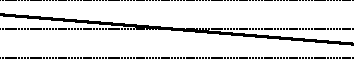
\includegraphics{images/contours-statement.pdf}%
	} //
	\gla Ang @ gihayo {} @ Pintemis minganeri-hen yona.//
	\glb ang= giha-yo Ø= Pintemis mingan-eri=hen yona //
	\glc \AgtT{}= blow-\TsgN{} \Top{}= {North Wind} ability-\Ins{}=all
		\TsgN{}.\Gen{}. //
	\glft `The North Wind blew with all of his might.' //
\endgl\xe

\subsubsection{Yes–no questions}
\index{questions|(}

Since Ayeri does not use a particle or word order to mark closed questions as 
such, intonation is used to mark the difference from a declarative statement. 
To achieve a strong contrast, questions exhibit gradually rising intonation:

\ex[belowexskip=0em]\begingl
	\glpreamble\adjustbox{valign=t}{%
		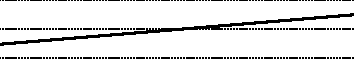
\includegraphics{images/contours-ynquestion.pdf}%
	} //
	\gla Ang @ gihayo {} @ Pintemis minganeri-hen yona? //
	\glb ang= giha-yo Ø= Pintemis mingan-eri=hen yona //
	\glc \AgtT{}= blow-\TsgN{} \Top{}= {North Wind} ability-\Ins{}=all
		\TsgN{}.\Gen{}. //
	\glft `Did the North Wind blow with all of his might?' //
\endgl\xe

\subsubsection{`Wh-' questions}

Unlike English\index{English}, Ayeri marks open questions with an in-situ question word.
Open questions are thus marked by the question word causing a sharp rise and 
fall in the overall contour of the question. The first half of the clause has 
the rising contour of a question, the second half has gradually falling pitch.

\ex[belowexskip=0em]\begingl
	\glpreamble\adjustbox{valign=t}{%
		
\includegraphics{images/contours-whquestion.pdf}%
	} //
	\gla Ang @ engyo mico sinya luga toya sam? //
	\glb ang= eng-yo mico sinya-Ø luga toya sam //
	\glc \AgtT{}= be.more-\TsgN{} strong who-\Top{} among \TplN{}.\Loc{}
		two //
	\glft `Who was the stronger of the two?' //
\endgl\xe

\index{questions|)}

\subsubsection{Lists}

List statements have the general gradual downward slope of declarative
statements, but the individual items can nonetheless be marked by a pitch rise
on the primary accent of each item.

\ex[belowexskip=0em]\begingl
	\glpreamble\adjustbox{valign=t}{%
		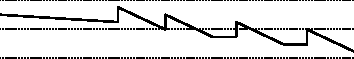
\includegraphics{images/contours-list.pdf}%
	} //
	\gla Le @ vacyeng seygo, disu, betay nay vasra. //
	\glb le= vac=yeng seygo-Ø disu-Ø betay-Ø nay vasra-Ø //
	\glc \PatTI{}= like=\TsgF{}.\Aarg{} apple-\Top{} banana-Ø berry-Ø and
		nut-Ø //
	\glft `She likes apples, bananas, berries and nuts.' //
\endgl\xe

\subsubsection{Complement and relative clauses}
\index{complement clause|(}
\index{relative clause|(}

Complement clauses\index{complement clause} are characterized by the short
spike at the end of the preceding main clause followed by a short break.
Together, these auditory clues signal the beginning of a new syntactic unit
within the context of the current sentence. This is broadly similar to list
statements. Otherwise, statements with complement clauses as well bear the
overall downward-sloping contour of declarative statements if included in such.

\ex\begingl
	\glpreamble\adjustbox{valign=t}{%
		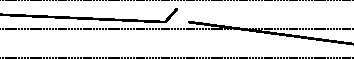
\includegraphics{images/contours-complement.pdf}%
	} //
	\gla Ang @ manga @ rantong, engyo mico sinyāng. //
	\glb ang= manga= ran=tong eng-yo mico sinya-ang //
	\glc \AgtT{}= \Prog{}= argue=\TplN{}.\Aarg{} be.more-\TsgN{} strong
		who-\Aarg{}//
	\glft `They were arguing who is stronger.' //
\endgl\xe

Relative clauses,\index{relative clause} on the other hand, do not receive 
special prosodic marking, but are treated the same as other basic sentence 
types. They display a continuous downward slope if part of a 
declarative statement, or a continuous upward slope if part of a question:

\pex[belowexskip=0em]
\a\begingl
	\glpreamble\adjustbox{valign=t}{%
		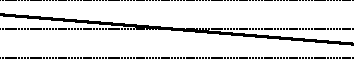
\includegraphics{images/contours-statement.pdf}%
	} //
	\gla Lugaya asāyāng si sitang-naykonyāng kong tovaya. //
	\glb luga-ya asāya-ang si sitang=naykon=yāng kong tova-ya mato //
	\glc pass-\TsgM{} traveler-\Aarg{} \Rel{} self=wrap=\TsgM{}.\Aarg{} 
		inside cloak-\Loc{} //
	\glft `A traveler passed who had wrapped himself into a cloak.' //
\endgl
\\

\a\label{ex:travelercoat}\begingl
	\glpreamble\adjustbox{valign=t}{%
		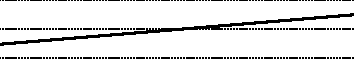
\includegraphics{images/contours-ynquestion.pdf}%
	} //
	\gla Adareng asāyās si le @ ninyāng tova? //
	\glb ada-reng asāya-as si le= nin=yāng tova-Ø //
	\glc that-\AargI{} traveler-\Parg{} \Rel{} \PatTI{}= wear=\TsgM{}.\Aarg{} 
		coat-\Top{} //
	\glft `Is that the traveler who wore the coat?' //
\endgl
\xe

\index{relative clause|)}
\index{complement clause|)}

\subsubsection{Contrast}

Ayeri uses a kind of topic system for highlighting constituents in a clause by
morphosyntactic means, but this is still different from emphasis on semantic
grounds, for example when the speaker wants to highlight a semantic difference
in the same syntactic position (compare focus, \autoref{subsec:focus}), as in
the following example, which presents a possible answer to the question posed in
(\ref{ex:travelercoat}):

\ex\begingl
	\glpreamble\adjustbox{valign=t}{%
		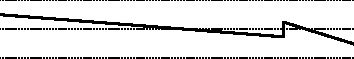
\includegraphics{images/contours-contrast.pdf}%
	} //
	\gla Adareng asāyās si le @ nin-yāng \upshape{kegan}. //
	\glb ada-reng asāya-as si le= nin=yāng kegan-Ø //
	\glc that-\AargI{} traveler-\Parg{} \Rel{} \PatTI{}= wear=\TsgM{}.\Aarg{} 
		hat-\Top{} //
	\glft `It is the traveler who wore the \emph{hat}.' //
\endgl\xe

We can see here a spike towards the end of the utterance where the word 
\xayr{kegnF}{kegan}{hat} is placed. This word receives extra stress for 
contrast with \xayr{tov}{tova}{coat}, which is what the other person had asked 
about.

\index{intonation|)}

\cleartorecto

% kate: word-wrap true;

\chapter{Writing system}
\index{Tahano Hikamu|(}

In the previous chapter, example words were given in Ayeri's script, \rayr{thno 
hikmu}{Tahano Hikamu}, wherever possible. Thus, it seems advisable to include a 
description of Ayeri's native writing system here as well. Literally, 
\rayr{thno hikmu}{Tahano Hikamu} means `Round Script' (script round), which is 
an old formation based on the word \xayr{thnF/}{tahan-}{write} that  stuck. The 
current word for `script' is \xayr{thnnF}{tahanan}{writing}. Tahano Hikamu was 
originally named thus because of an earlier draft for a script that never made 
it very far beyond the drawing board and which was a lot more angular and boxy, 
see \autoref{fig:boxyhikamu}---Tahano Hikamu was a lot more bubbly in 
comparison, especially early on (\autoref{fig:th2005}).\footnote{Unfortunately, 
there is no documentation of the Box script surviving that I know 
of.}\index{Box script}

\begin{figure}[tp]
\caption{Box script and Hikamu}

\begin{minipage}{.5\linewidth}

\includegraphics[width=\linewidth]{images/hinya-300dpi-clip.png}
\subcaption{Old and aborted draft: Box script}
\label{fig:boxy}
\end{minipage}
~
\begin{minipage}{.5\linewidth}
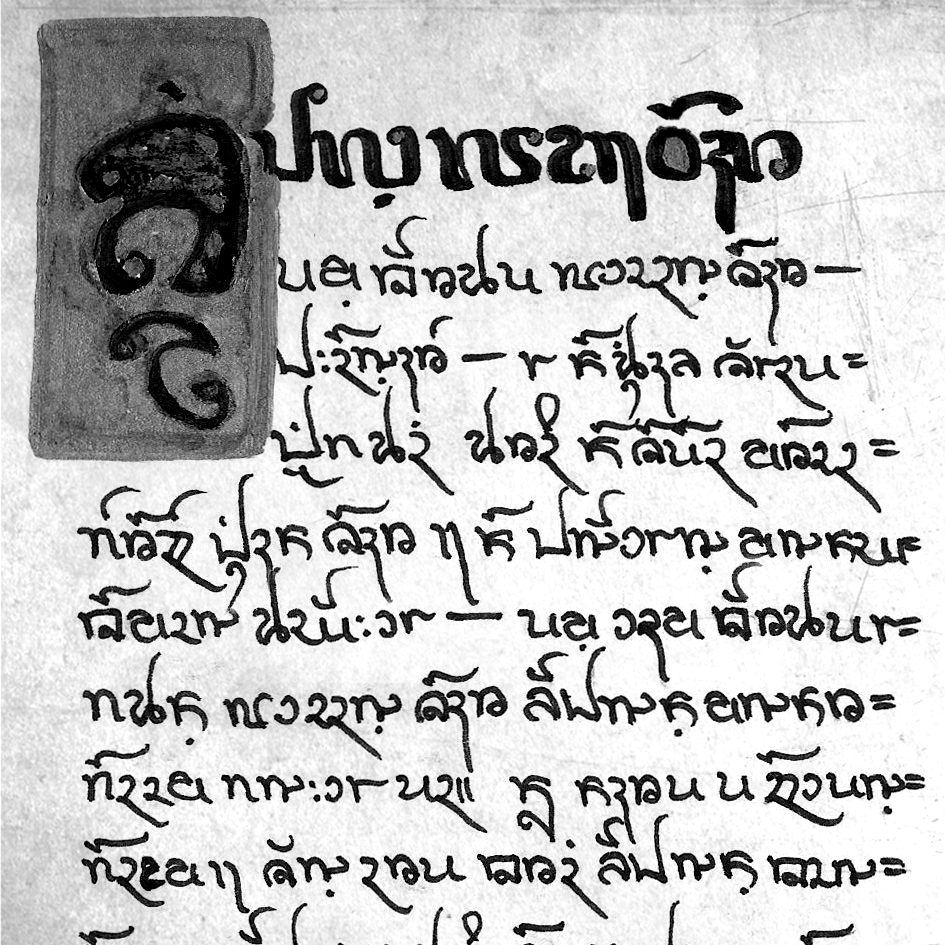
\includegraphics[width=\linewidth]{images/tahano-300dpi-bw-clip.png}
\subcaption{Ayeri's native script: Tahano Hikamu}
\end{minipage}

\label{fig:boxyhikamu}
\end{figure}

As we have seen in the previous chapter, Ayeri's prosody strongly emphasizes 
the syllable as a unit. Thus, it is not a surprise that Ayeri's native script,
Tahano Hikamu, is an alphasyllabary similar to the Brāhmī alphabets of 
India and Southeast Asia \parencites{salomon1996}{court1996}.\index{Brāhmī 
scripts} Scripts like these are 

\blockcquote[376]{salomon1996}{based on the unit of the graphic 
\enquote{syllalbe} […], which by definition always ends with a vowel (type V, 
CV, CCV, etc.). Syllables consisting of a vowel only (usually at the beginning 
of a word or sentence) are written with the \emph{full} or \emph{initial vowel 
signs} […]. But when, as is much more frequently the case, the syllable 
consists of a consonant followed by a vowel, the vowel is indicated by a 
diacritic sign attached to the basic sign for the consonant […].}

For Tahano Hikamu the definition that a syllable consisting only of a vowel is 
written with an initial vowel sign is only true under certain circumstances, as 
we will see below. Moreover, Brāhmī scripts are often characterized by 
conjuncts of clustered consonants which may become quite large and sometimes 
behave in an idiosyncratic way. Consonant conjuncts like Devanāgarī {\FS 
त्व}~\orth{tva} from {\FS त}~\orth{ta} + {\FS व}~\orth{va} or idiosyncratic 
conjuncts like {\FS क्ष} \orth{kṣa} for {\FS क} \orth{ka} + {\FS ष} \orth{ṣa} 
are not known in Tahano Hikamu, however. Tahano Hikamu also does not know 
subscript notation for consonant clusters and special diacritics marking coda 
consonants like in Javanese \citep[478--479]{kuipersmcdermott1996}. This does 
not mean, however, that final consonants are simply omitted in writing, since 
closed syllalbes are reasonably common enough in Ayeri to warrant indicating 
them. Thus, there is \textcquote[476]{kuipersmcdermott1996}{a special mark to 
eliminate the vowel of the previous syllable, thereby leaving a consonant in a 
syllable-final position.} That is, a diacritic exists which marks the absence 
of an inherent vowel, rendering the syllable consonant-only.

Another difference from Brāhmī-family scripts is that vowel length and 
diphthongs in [ɪ] are indicated by dedicated diacritics, so the long vowels 
are not doubled versions of their short counterparts. Like in 
Kharoṣṭhī---another historically important ancient script of India---initial 
vowels are not represented by unique graphemes but they are all written like 
post-consonantal vowel diacritics \citep[377]{salomon1996}, though in Tahano 
Hikamu with a charcter without an inherent sound value. For this reason, 
the character is indicated in the table below as \ayr{ʔ} /Ø/; its native name 
is \xayr{rnYn}{ranyan}{nothing}.\footnote{I will give the native names of 
graphemes here, but will refer to them by their English names for clarity in 
the running text.} Similar to a number of Brāhmī scripts, Tahano Hikamu puts 
diacritics not only below or above consonant bases, but also before them. This, 
however, is not limited to vowel graphemes as in Devanāgarī {\FS ि}~\orth{i} or 
Javanese \smash{\fontspec{Tuladha Jejeg}[Script=Javanese, 
Scale=MatchLowercase]ꦺ}~\orth{e, é/è} 
\citep[478]{kuipersmcdermott1996}.\footnote{\citet{kuipersmcdermott1996} do not 
say, but it looks likely to me that both are related, since they are both 
functionally the only prepended vowel diacritics and both represent a high front 
sound.}

\section{Consonants}
\index{consonants|(}

Tahano Hikamu is mainly based on consonant bases that are modified by 
diacritics. Since the vowel /a/ is so highly frequent in Ayeri, it is also the 
vowel that is \fw{inherent} to every consonant grapheme if not further modified 
by vowel diacritics. Consonant letters are simply referred to as \textit{pa, ta, 
ka, ...} \autoref{fig:consonants} displays all the main consonants. The 
customary collation is---similar to the IPA table---roughly grouping the letters 
according to their sound value by anteriority (front → back) and sonority (low → 
high). The script is monocameral, that is, there is no distinction between 
capital letters and minuscule letters as in the Latin, Greek, Cyrillic, 
Georgian, and Armenian alphabet. It is also written in lines from left to right.

% \begin{center}\itshape
% 	pa, ta, ka;\\
% 	ba, da, ga;\\
% 	ma, na, nga;\\
% 	va, sa, ha;\\
% 	ra, la, ya;\\
% 	Ø.\\
% \end{center}

\begin{figure}[ht]
\caption{The consonant graphemes of Tahano Hikamu}

\begin{tabu} to \linewidth{X[c] X[c] X[c] X[c] X[c] X[c]}
\toprule
\tableheaderfont	/pa/ & /ta/ & /ka/ & /ba/ & /da/ & /ga/ \\
\rowfont{\Tagati\huge}	p & t & k & b & d & g \\

\midrule

\tableheaderfont	/ma/ & /na/ & /ŋa/ & /va/ & /sa/ & /ha/ \\
\rowfont{\Tagati\huge}	m & n & N & v & s & h \\

\midrule

\tableheaderfont	/ra/ & /la/ & /ja/ & /Ø/ \\
\rowfont{\Tagati\huge}	r & l & y & ʔ \\

\bottomrule
\end{tabu}
\label{fig:thcons}
\end{figure}

\ayr{ʔ}, which in Ayeri has no sound value but is used as a base for initial 
vowels, may also serve as the character for /ʔa/. What is, moreover, 
interesting about \ayr{N}~\orth{nga} is that even though before, /ŋ/ was treated 
strictly as a coda consonant in the previous chapter, it is in fact treated as 
an onset consonant in writing if a vowel is following:

\ex[lingstyle=thex]\begingl
	\gla \ayr{p}	$+$	\ayr{NisF} //
	\glb /pa/	{}	/ŋis/ //
	\glft \rayr{\larger pNisF}{pangis} /paŋ.is/ `money' //
\endgl\xe

Tahano Hikamu knows a few ligatures. First of all, when two \ayr{n} \orth{na} 
are in succession within a word, they will form a ligature \ayr{nn} \orth{nana}:

\ex[lingstyle=thex]\begingl
	\gla \ayr{n}	$+$	\ayr{n}	→	\ayr{nn} //
	\glb /na/	{}	/na/	{}	/nana/ //
\endgl\xe

\noindent This is distinct from conjuncts like in Devanāgarī et al., though, 
since the unmodified sound value will still be /nana/, not */nna/, so the 
inherent vowel of each \ayr{n} \orth{na} is not deleted, and each \ayr{n} 
\orth{na} retains the ability to be modified by diacritics. Tahano Hikamu also 
has a few ligatures of the kind you would find in Brāhmī scripts, however:

\pex
	\a \ayr{\larger q}~\orth{kwa} ← \ayr{\larger k}~\orth{ka} + 
		\ayr{\larger v}~\orth{va},
	\a \ayr{\larger T}~\orth{tsa} ← \ayr{\larger t}~\orth{ta} + 
		\ayr{\larger s}~\orth{sa}, and 
	\a \ayr{\larger x}~\orth{ksa} ← \ayr{\larger k}~\orth{ka} + 
		\ayr{\larger s}~\orth{sa}.
\xe

\noindent These conjunct letters are, however, not normally employed by Ayeri. 
\autoref{fig:thconsadd} shows all additional consonants, added to write other 
languages. Individual languages may adapt the sound values slightly to fit their 
own purposes.

\begin{figure}[ht]
\caption{Additional consonant graphemes of Tahano Hikamu}

\begin{tabu} to \linewidth{X[c] X[c] X[c] X[c] X[c] X[c]}
\toprule
\tableheaderfont	/fa/ & /wa/ & /tsa/ & /za/ & /ʃa/ & /ʒa/ \\
\rowfont{\Tagati\huge}	f & w & T & z & S & Z \\

\midrule

\tableheaderfont	/ça/ & /ksa/ & /kwa/ & /xa/ & /ɣa/ \\
\rowfont{\Tagati\huge}	C & x & q & X & G \\

\bottomrule
\end{tabu}
\label{fig:thconsadd}
\end{figure}

\index{consonants|)}

\section{Vowels}
\index{vowels|(}

As mentioned above, vowels are written as diacritics that are added to 
consonants. In principle, every consonant has two slots for vowels, a primary 
one atop it, and a secondary one below it. Vowels added to consonants in 
the primary slot delete their inherent /a/:

\ex[lingstyle=thex]\begingl
	\gla \ayr{p}	→	\ayr{pe} //
	\glb /pa/	{}	/pe/ //
\endgl\xe

\begin{figure}[th]
\caption{Primary vowel graphemes of Tahano Hikamu}

\begin{tabu} to \linewidth{H[c] X[c] X[c] X[c] X[c] X[c] X[c] X[c]}
\toprule
\tableheaderfont

	& /i/
	& /e/
	& /a/
	& /o/
	& /u/
	& /ə/
	& /aʊ/
	\\
	
\toprule
	
Diaritics
	& \Tagati\huge *i
	& \Tagati\huge *e
	& \huge ({\Tagati *a})
	& \Tagati\huge *o
	& \Tagati\huge *u
	& \Tagati\huge *ə
	& \Tagati\huge *au
	\\

\midrule

Independent
	& \Tagati\huge I
	& \Tagati\huge E
	& \Tagati\huge A
	& \Tagati\huge O
	& \Tagati\huge U
	& \Tagati\huge Ə
	& \Tagati\huge AU
	\\

\bottomrule
\end{tabu}
\label{fig:thvowstop}
\end{figure}

\autoref{fig:thvowstop} gives the primary vowel signs. Of the vowel signs given 
there, only \ayr{*ə}~\orth{ə} is not used in Ayeri. \ayr{*au}~\orth{au} is the 
only diphthong for which a dedicated grapheme exists, even though its occurrence 
is rather limited. The independent vowel graphemes are used at the beginning of 
words or inside words when there is no other way to spell the vowel, which is 
occasionally the case for secondary vowels. Secondary vowels are vowels that are 
not parts of diphthongs (even though another language might use them to spell 
diphthongs that are not covered by default), but follow the vowel of a syllable 
directly. They are attached underneath a consonant base, for example:

\ex[lingstyle=thex]\begingl
	\gla \ayr{y}	→	\ayr{ye}	→	\ayr{ye\_a} //
	\glb /ja/	{}	/je/		{}	/jea/ //
\endgl\xe

In fact, the principle that every consonant base with its diacritics represents 
one syllable is slightly violated here, which is also the reason why secondary 
vowels very occasionally need to be spelled as independent vowels, for example 
when the secondary vowel is long, as in the word \xayr{ruAAnF}{ruān}{duty}:

\ex[lingstyle=thex]\label{ex:rwaa}\begingl
	\gla \ayr{ru}	→	\ayr{ruAA}	\quad	(\,\ayr{ruu\_a}) //
	\glb /ru/	{}	/rwaː/ 		\quad	/ruːa/ //
\endgl\xe

Example (\ref{ex:rwaa}) uses a diacritic, \ayr{*aa}, to indicate length. If 
is put directly under \rayr{ru}{ru} (the \ayr{*\_a} diacritic moves down where 
it is not in the way), the syllable will incorrectly spell /ruːa/ instead of 
the intended /ruaː/. This is because diacritics modify consonants and primary 
vowels, but there is no way to modify a secondary vowel directly. 
\autoref{fig:thvowsbot} gives a list of secondary vowels corresponding to that 
of primary vowels above. The vowels as well are just referred to by their sound 
value; `primary' and `secondary', `superscript' and `subscript' or `upper' and 
`lower' may be chosen to disambiguate their positions; the native names may use 
\xayr{Iraj}{iray}{high} and \xayr{Ejr}{eyra}{low} to disambiguate, so \rayr{E 
Irj}{e iray} denotes the superscript \orth{e} diacritic while \rayr{E Ejr}{e 
eyra} denotes its subscript counterpart.

\begin{figure}[ht]
\caption{Secondary vowel graphemes of Tahano Hikamu}

\begin{tabu} to \linewidth{X[c] X[c] X[c] X[c] X[c] X[c] X[c]}
\toprule
\tableheaderfont	/i/ & /e/ & /a/ & /o/ & /u/ & /ə/ & /aʊ/ \\
\rowfont{\Tagati\huge}	*\_i & *\_e & *\_a & *\_o & *\_u & *\_ə & *\_au \\

\bottomrule
\end{tabu}
\label{fig:thvowsbot}
\end{figure}

As a further exception, those consonant bases with an ascender 
(\ayr{k}~\orth{ka}, \ayr{d}~\orth{da}, \ayr{C}~/ça/) move the primary vowel to 
the secondary slot below the consonant by default while indicating the vacancy 
of the primary slot at the top with a dot. This is done to avoid crossing the 
ascender of the consonant with a vowel diacritic:

\ex[lingstyle=thex]\begingl
	\gla \ayr{k}	→	\ayr{k\_i}	→	\ayr{ki} //
	\glb /ka/	{}	/ka.i/		{}	/ki/ //
\endgl\xe

If the primary vowel slot were not silenced by the \ayr{*\_F} diacritic, it 
could reasonably be assumed that the consonant is not losing its inherent /a/ 
and the vowel below the consonant indicates a secondary vowel, spelling /CaV/. 
If, however, a secondary vowel is \emph{actually} added, primary and secondary 
vowels will be assigned the regular primary and secondary slots, respectively, 
again (\ref{ex:kie}). This condition also holds true for subscript diacritics 
(\ref{ex:kii}).

\pex[lingstyle=thex]
\a\label{ex:kie}\begingl
	\gla \ayr{ki}	→	\ayr{ki\_e} //
	\glb /ki/	{}	/ki.e/ //
\endgl

\a\label{ex:kii}\begingl
	\gla \ayr{ki}	→	\ayr{kii} //
	\glb /ki/	{}	/kiː/ //
\endgl

\xe

The order of secondary vowels and subscript diacritics is iconic insofar as 
it follows the order of sounds in the syllable. Thus, secondary vowels appear 
below the consonant-doubling diacritic, \ayr{*F*}, while they appear above the 
syllable-final homorganic nasal diacritic, \ayr{*\_M}:

\pex[lingstyle=thex]\label{ex:subscrord}
\a\begingl
	\gla \ayr{pFp}	→	\ayr{pFpe\_a} //
	\glb /ppa/	→	/ppea/ //
\endgl

\a\begingl
	\gla \ayr{peM}	→	\ayr{pe\_aM} //
	\glb /peN/	→	/peaN/ //
\endgl
\xe

\index{vowels|)}

\section{Diacritics}
\index{diacritics|(}

We have already encountered a few diacritics, though Tahano Hikamu comes with 
a lot more, some of which undergo non-trivial positioning and repositioning 
rules. As vowels are primarily expressed as superscripts, diacritics are 
primarily realized as subscripts, so in the following I will first describe 
subscript diacritics; then prepended diacritics, which Ayeri also has a number 
of, both as graphemes in their own right and as allographs of other subscript 
diacritics; and then, lastly, superscript diacritics.

\subsection{Subscript diacritics}

\begin{sidewaysfigure}[p]
\caption{Bottom-attaching diacritics of Tahano Hikamu}
\begin{tabu} to \linewidth{>{\Tagati\huge}X[1] X[8l] X[16l] X[12l]}
\toprule
\tableheaderfont

	& Native name
	& Function
	& Example
	\\
	
\toprule

\tablesubheaderfont\multicolumn{4}{c}{L~a~r~g~e~{ }~d~i~a~c~r~i~t~i~c~s}\\

\midrule

*aa
	& \xayr{tupsti}{tupasati}{long-maker}
	& Lengthens the primary vowel of the syllable
	& \rayr{p}{pa} → \rayr{paa}{pā}
	\\

\midrule
	
*Y
	& \xayr{y Ejr}{ya eyra}{low ya}
	& \orth{ya} following another consonant, also across syllables. Marks 
		palatalization of \ayr{t}~\orth{ta}, \ayr{d}~\orth{da}, 
		\ayr{k}~\orth{ka}, \ayr{g}~\orth{ga} and \ayr{y}~\orth{ya} in 
		Ayeri.
	& \rayr{Ar}{ara} → \rayr{ArY}{arya}; \rayr{t}{ta} → \rayr{tY}{ca}
	\\
	
\midrule
	
*J
	& \xayr{riNy}{ringaya}{raiser}
	& Palatalizes a consonant (not used in Ayeri)
	& \rayr{t}{ta} → \ayr{tJ} /tʲa/, /tʃa/
	\\
	
\midrule
	
*H
	& \xayr{UlNy}{ulangaya}{breather}
	& Aspiration or frication of a consonant (not used in Ayeri)
	& \rayr{t}{ta} → \ayr{tH} /tʰa/, {\addfontfeature{RawFeature=+mgrk}/θa/}
	\\
	
\midrule
	
*\hspace{-.25em}ˀ
	& \xayr{rjpaay Ejr}{raypāya eyra}{low~stopper}
	& Glottal stop coda or glottalization of a consonant (consonant letters 
		with ascenders; not used in Ayeri)
	& \rayr{k}{ka} → \ayr{kQ} /kaʔ/; \rayr{d}{da} → \ayr{dQ} /d’a/
	\\

\midrule

\tablesubheaderfont\multicolumn4{c}{S~m~a~l~l~{ }~d~i~a~c~r~i~t~i~c~s}\\

\midrule

*F
	& \xayr{goMdy}{gondaya}{extinguisher}
	& Deletes the inherent /a/ of a consonant, e.g. in consonant clusters 
		or closed syllables
	& \rayr{pr}{para} → \rayr{pFr}{pra}, \rayr{prF}{par}
	\\
	
\midrule
	
*M
	& \xayr{vinaati}{vināti}{nasalizer}
	& Indicates a homorganic nasal or nasalizes the vowel, depending on the 
		language
	& \rayr{pd}{pada} → \rayr{pMd}{panda} /panda/ or /pãda/
	\\
	
\midrule
	
*F*
	& \xayr{kusNisaati}{kusangisāti}{duplicator}
	& Indicates a geminated or otherwise double consonant
	& \rayr{pl}{pala} → \rayr{plFl}{palla}
	\\

\bottomrule
\end{tabu}
\label{fig:thdiabot}
\end{sidewaysfigure}

\autoref{fig:thdiabot} shows the bottom-attaching diacritics. The `large 
diacritics' cause the secondary slot of consonants to move down below the 
diacritic. `Small diacritics' can attach in this place as well as secondary 
vowels, as does the homorganic nasal diacritic \ayr{*M} in this 
diacritic-fraught example:

\ex[lingstyle=thex]\label{ex:caampuluy}\begingl
	\gla \ayr{tYaan} $+$ \ayr{puluj} → \ayr{tYaaMpuluj} //
	\glb {/ˈtʃaːn/} {} {/puˈlʊɪ/} {} {/ˌtʃaːmpuˈlʊɪ/} //
% 	\glc \xayr{tYaanF}{cān}{love} {} \xayr{puluj}{puluy}{opposite} {}
% 		\xayr{tYaaMpuluj}{cāmpuluy}{heterosexual} //
	\glft \xayr{\larger tYaaMpuluj}{cāmpuluy}{heterosexual} //
\endgl\xe

It also needs to be noted that diacritics like \ayr{*Y} are applied 
progressively to words as a whole, not stopping at morpheme and syllable 
boundaries, so even though \tayr{toryeng}{she sleeps} may be composed of 
\xayr{torF/}{tor-}{sleep} + \rayr{/yeNF}{-yeng} (=\TsgF{}.\Aarg{}) and 
syllabifies as /tor.ˈjeŋ/, the spelling is not *\,\ayr{torF\zwsp{}yeNF} as one 
might expect, but \ayr{torYeNF}.

Even though the primary position for small diacritics is underneath consonants, 
the diacritic deleting the inherent vowel, \ayr{*F}, very commonly also 
appears after a consonant letter at the end of words:

\ex[everygla=\Tagati\Large,everyglb=\itshape]\begingl
	\gla y nimFreN\thafterdot{} pNn\thafterdot{} 
		nraanFyen. //
	\glb Ya nimreng pangan narānyena. //
	\glc Ya nim-reng pangan-Ø narān-ye-na //
	\glc \LocT{} appear=\TsgI{}.\Aarg{} end-\Top{} word-\Pl{}-\Gen{} //
	\glft `It appears at the end of words.' //
\endgl\xe

This strategy is advantageous in that Tahano Hikamu leaves very little space 
between individual words: \ayr{y nimFreN\thafterdot{} pNn\thafterdot{} 
nraanFyen.} With the dot after the consonant, word boundaries are more visible.

\subsection{Prepended diacritics}

Example (\ref{ex:caampuluy}) leads us directly to the next class of 
diacritics---ones that are prepended to the consonant letter, either because 
they are simply placed there or because of allography. Let us first list those 
diacritics that appear in front of consonants obligatorily 
(\autoref{fig:thdiapreobl}).

\begin{figure}[htp]
\caption{Obligatorily prepended diacritics of Tahano Hikamu}
\begin{tabu} to \linewidth{>{\Tagati\huge}X[1] X[8l] X[16l] X[12l]}
\toprule
\tableheaderfont

	& Native name
	& Function
	& Example
	\\
	
\toprule

*j
	& \xayr{leMtMkusNF}{lentan\-kusang}{double-\allowbreak{}sound}
	& Marks a diphthong with /ɪ/
	& \rayr{pe}{pe} → \rayr{pej}{pey}
	\\
	
\midrule

*\_:
	& \xayr{tilmy}{tilamaya}{changer}
	& Marks raised vowels (i.e. umlaut; not used in Ayeri)
	& \rayr{po}{po} → \ayr{po\_:}~/pø/
	\\
	
\midrule

*R
	& \xayr{hiymy}{hiyamaya}{roller}
	& Marks retroflex consonants (not used in Ayeri)\footnotemark
	& \rayr{t}{ta} → \ayr{tR}~/ʈa/
	\\

\bottomrule
\end{tabu}
\label{fig:thdiapreobl}
\end{figure}

\footnotetext{In a Tahano Hikamu orthography I devised for English once, 
\ayr{*R} was used for /ɚ/, as in the \textsc{nurse} vowel in American English: 
\rayr{nRsF}{nurse}.}

\begin{figure}[htp]
\caption{Allographically prepended diacritics of Tahano Hikamu}
\begin{tabu} to \linewidth{>{\Tagati\huge}X[1] X[8l] X[16l] X[12l]}
\toprule
\tableheaderfont

	& Native name
	& Function
	& Example
	\\
	
\toprule

ː*
	& \xayr{tupsti mrinF}{tupasati marin}{anterior long-maker}
	& Lengthens the primary vowel of the syllable
	& \rayr{sY}{sya} → \rayr{sYaa}{syā},\newline
		\rayr{n}{na} → \rayr{naa}{nā}
	\\
	
\midrule

ʲ*
	& \xayr{y mrinF}{ya marin}{anterior ya}
	& \orth{ya} following another consonant, also across syllables.
	& \rayr{n}{na} → \rayr{nY}{nya}
	\\
	
	
	& \xayr{riNy mrinF}{ringaya marin}{anterior raiser}
	& Also used as an allograph for the palatalization proper diacritic.
	& \ayr{sH}~/sʰa/ → \ayr{sHY}~/sʰʲ/
	\\
	
\midrule

ʰ*
	& \xayr{UlNy mrinF}{ulangaya marin}{anterior breather}
	& (Pre-)Aspiration or frication of a consonant (not used in Ayeri)
	& \rayr{N}{nga} → \ayr{NH} /ŋʰa/;\newline
		\rayr{t}{ta} → \ayr{ʰt}~/ʰta/
	\\

\bottomrule
\end{tabu}
\label{fig:thdiapreallo}
\end{figure}

As \autoref{fig:thdiapreobl} shows, the only obligatorily prepended diacritic 
that Ayeri uses is the one that marks diphthongs, \ayr{*j}.\index{diphthongs} 
It needs to be noted here that \ayr{*j} changes into \ayr{y}~\orth{ya} proper 
when a vowel follows, but stays \ayr{*j} when a \ayr{y}~\orth{ya} follows:

\pex
	\a \xayr{\larger hdj}{haday}{hero} → 
		\ayr{\larger hdyNF} (*\,\ayr{\larger hdjANF}) \fw{hadayang}
		`the hero' (hero-\Aarg{});
	\a \xayr{\larger tipuj}{tipuy}{grass} → 
		\ayr{\larger tipujy} (*\,\ayr{\larger tipuyY}) \fw{tipuyya} `in 
		the grass' (grass-\Loc{}).
\xe

Besides \ayr{*j}, there are also a number of diacritics that are also 
obligatorily prepended to consonants, but do so as context-sensitive allographs 
(\autoref{fig:thdiapreallo}). The selection of the variant diacritics is not 
random or up to the aesthetic eye of the writer (even though the device itself 
is certainly a matter of aesthetics), but it is governed by rules. The 
prepended forms listed in \autoref{fig:thdiapreallo} are thus triggered 

\begin{enumerate}
\item when there is no stem or bowl for the regular subscript diacritic to 
	attach to, which is the case for \ayr{n}~\orth{na}, \ayr{N}~\orth{nga}, 
	\ayr{v}~\orth{va}, and \ayr{w}~\orth{wa}:
	
	\begin{multicols}{2}
	\pex[lingstyle=thex,]\label{ex:stemless}
	\a\begingl
		\gla \ayr{n} → \ayr{naa} //
		\glb /na/ {} /naː/ //
	\endgl
	
	\a\begingl
		\gla \ayr{N} → \ayr{Naa} //
		\glb /ŋa/ {} /ŋaː/ //
	\endgl
	
	\a\begingl
		\gla \ayr{v} → \ayr{vaa} //
		\glb /va/ {} /vaː/ //
	\endgl
	
	\a\begingl
		\gla \ayr{w} → \ayr{waa} //
		\glb /wa/ {} /waː/ //
	\endgl
	
	\xe
	\end{multicols}

\item when a large subscript diacritic would be added after another large 
	subscript diacritic---this position can only be occupied once, so 
	further large subscripts are prepended:
	
	\ex[lingstyle=thex,everygla=\normalsize,everyglb=\upshape\Large,
		aboveglcskip=0.5em,numoffset=\leftmargin]\label{ex:stacking}
	\begingl
		\gla {} {$+$ \ayr{*H}} {} {$+$ \ayr{*Y}} {} {$+$ \ayr{*i}} {}
			{$+$ \ayr{*aa}} {} //
		\glb \ayr{t} → \ayr{tH} → \ayr{tHY} → \ayr{tHYi} → 
			\ayr{tHYii} //
		\glc /ta/ {} /tʰa/ {} /tʰja/ {} /tʰji/ {} /tʰjiː/ //
	\endgl\xe
	
	The order of diacritics follows the logic of the respective 
	language's phoneme inventory, so if there are, for example, 
	retroflex consonants and both dental and retroflex consonants can be 
	aspirated, retroflexion would be marked first, then aspiration. If 
	there is a palatalization contrast on top of this, the diacritic would 
	be added after aspiration.
	
	When adding large diacritics to stemless consonants, they are prepended 
	from the beginning, as we saw in (\ref{ex:stemless}), and just like in 
	(\ref{ex:stacking}), this principle continues:
	
	\ex[lingstyle=thex,everygla=\normalsize,everyglb=\upshape\Large,
		aboveglcskip=0.5em,numoffset=\leftmargin]
	\begingl
		\gla {} {$+$ \ayr{*Y}} {} {$+$ \ayr{*aa}} {} {$+$ \ayr{*j}} 
			{} //
		\glb \ayr{n} → \ayr{nY} → \ayr{nYaa} → \ayr{nYaaj} //
		\glc /na/ {} /nja/ {} /njaː/ {} /njaːɪ/ //
	\endgl\xe

\item with consonants directly following \ayr{n}~\orth{na}, to avoid a clash 
	with its swash:
	
	\ex[lingstyle=thex,numoffset=\leftmargin]
	\begingl
		\gla \ayr{n} $+$ \ayr{paa} → \ayr{npaa} \quad
			(*\,\ayr{n\zwsp{}paa}) //
		\glb /na/ {} /paː/ {} /napaː/ {} {} //
	\endgl\xe
	
	An exception to this exception occurs, however, when the consonant is 
	not directly following. In this case, no reordering happens, only 
	\ayr{n}~\orth{na} \emph{may} reduce its swash in size to accommodate the 
	following prepended diacritic:\footnote{The font I am using here is 
	designed so that the reduced combination looks nicer, but if unreduced, 
	\ayr{n}~\orth{na}'s swash is not so long as to cross the descender of 
	\ayr{*j} either in this particular case.}
	
	\pex[lingstyle=thex,numoffset=\leftmargin]
	\begingl
		\gla \ayr{n} $+$ \ayr{pj} → \ayr{npj} \quad
			(\ques{}\ayr{n\zwsp{}pj}) //
		\glb /na/ {} /paɪ/ {} /napaɪ/ {} {} //
	\endgl\xe
	
\item in other cases where a clash of subscript diacritics needs to be avoided:

	\ex[lingstyle=thex,numoffset=\leftmargin]
	\begingl
		\gla \ayr{di} $+$ \ayr{paa} → \ayr{diːp} \quad 
			(*\,\ayr{dipaa}) //
		\glb /di/ {} /paː/ {} /dipaː/ {} {} //
	\endgl\xe
	
	Alternatively, the following solution is permissible:
	
	\ex[lingstyle=thex,numoffset=\leftmargin]%
	\begingl
		\gla \ayr{di} $+$ \ayr{paa} → 
		% Due to negligence when coding the Tahano Hikamu font, I did 
		% not build in a way to manually put a diacritic on top of ⟨ka⟩ 
		% and ⟨da⟩, thus I need to put it on the letter with LaTeX 
		% commands, which is very clumsy. Younger self: shame on you!
		\ayr{d\hspace{-.3em}\raisebox{1.5ex}{\zwsp i}\hspace{.3em}%
			paa} //
		\glb /di/ {} /paː/ {} /dipaː/ //
	\endgl\xe
	
	When two long syllables follow each other, as in 
	\tayr{bāmā}{mom-and-dad}, one of the length diacritics should 
	definitely be pulled to the front:
	
	\ex[lingstyle=thex,everyglb=\upshape\Large,aboveglcskip=0.5em,
	numoffset=\leftmargin]
	\begingl
		\gla {} \ayr{baa} $+$ \ayr{maa} → \ayr{baaːm} \quad 
			(\ques{}\ayr{baamaa}) //
		\glb {\normalsize or:\quad} \ayr{baa} $+$ \ayr{maa} → 
			\ayr{ːbmaa} //
		\glc {} /baː/ {} /maː/ {} /baːmaː/ //
	\endgl
	
	\xe

\end{enumerate}

\subsection{Superscript diacritics}

Ayeri's standard position for diacritics is below consonants, but sometimes it 
is nicer to put them on top, especially for the letter \ayr{n}~\orth{na} due to 
its swash, as well as for \ayr{v}~\orth{va} since the space below its flag is 
empty otherwise, thus not providing much of a visual connection. The only 
diacritic that is normally attaching to the top of consonants is that for the 
glottal stop---we have already encountered its subscript allograph earlier. 
Since Ayeri's phoneme inventory does not possess a phonemic glottal stop or 
glottalization, this diacritic is not used in Ayeri. The list of superscript 
diacritics is given in \autoref{fig:thdiatop}.

\begin{figure}[htp]
\caption{Superscript diacritics of Tahano Hikamu}
\begin{tabu} to \linewidth{>{\Tagati\huge}X[1] X[8l] X[16l] X[12l]}
\toprule
\tableheaderfont

	& Native name
	& Function
	& Example
	\\
	
\toprule

*\_F
	& \xayr{goMdy liNF}{gondaya ling}{upper extinguisher}
	& Deletes inherent /a/ of consonant, e.g. in consonant clusters or 
		closed syllables
	& \rayr{vr}{vara} → \rayr{v\_Fr}{vra}
	\\
	
\midrule

*\_M
	& \xayr{vinaati liNF}{vināti ling}{upper nasalizer}
	& Indicates a homorganic nasal or nasalizes the vowel, depending on 
		language/context
	& \rayr{nd}{naka} → \rayr{nMk}{nanka} /naŋka/ or /nãka/
	\\
	
\midrule

*̔
	& \xayr{kusNisaati liNF}{kusangisāti ling}{upper duplicator}
	& Indicates a geminated or otherwise double consonant
	& \rayr{pn}{pana} → \rayr{pnFn}{panna}
	\\
	
\midrule

*Q
	& \xayr{rjpaay}{raypāya}{stopper}
	& Glottal stop coda or glottalization of a consonant (not used in Ayeri)
	& \rayr{t}{ta} → \ayr{tQ} /taʔ/;\newline
		\rayr{s}{sa} → \ayr{sQ} /s’a/
	\\

\bottomrule
\end{tabu}
\label{fig:thdiatop}
\end{figure}

At times, it may be necessary to attach both a superscript diacritic and a 
vowel sign above a consonant. In this case, the consonant-modifying diacritic 
is placed first and the vowel diacritic on top of it---this is exactly 
equivalent to the rule exemplified for subscript diacritics in 
(\ref{ex:subscrord}).

\index{diacritics|)}

\section{Numerals}
\index{numerals!digits|(}

Ayeri uses a duodecimal number system, that is, a system based on the powers of
of 12, which is a typological rarity.\footnote{And one possibly overrepresented 
by fictional languages due to its rarity in natural languages.} There is a 
digit for zero, so the system is positional, like the Hindu–Arabic digits used 
by the Latin alphabet. The numerals for the numbers from 1 to 12 are shown in 
\autoref{fig:thnum}.

\begin{figure}[ht]
\caption{The numerals of Tahano Hikamu}

\begin{tabu} to \linewidth{X[c] X[c] X[c] X[c] X[c] X[c]}
\toprule
\tableheaderfont	1 & 2 & 3 & 4 & 5 & 6 \\
\rowfont{\Tagati\huge}	1 & 2 & 3 & 4 & 5 & 6 \\

\midrule

\tableheaderfont	7 & 8 & 9 & A & B & 10 \\
\rowfont{\Tagati\huge}	7 & 8 & 9 & ¹ & ² & 10 \\

\bottomrule
\end{tabu}
\label{fig:thnum}
\end{figure}

% How are the various mathematical operations indicated, especially the basic 
% ones: addition, subtraction, multiplication, division, equality?

\index{numerals!digits|)}

\section{Punctuation and abbreviations}
\index{punctuation|(}

Tahano Hikamu's system of manipulating the sound of syllables is very 
sophisticated, so it comes as no surprise that it is also host of a large 
number of punctuation marks. \autoref{fig:thpunctcom} lists the ones commonly 
encountered, \autoref{fig:thpunctuncom} the ones not so commonly encountered.

\begin{figure}[htp]
\caption{Common punctuation marks of Tahano Hikamu}
\begin{tabu} to \linewidth{>{\Tagati\huge}X[2] X[8l] X[15.5l] X[11.5l]}
\toprule
\tableheaderfont

	& Native name
	& Function
	& Example
	\\
	
\toprule

.
	& \xayr{dnF}{dan}{dot}
	& Full stop
	& \xayr{sryaaNF.}{Sarayāng.}{He left.}
	\\
	
\midrule

/
	& \xayr{dnF/dnF}{dan-dan}{little dot}
	& A separator for small things, like clitics and abbreviations; 
		divides the constituents of reduplication
	& \xayr{Ad/nN}{ada-nanga}{this house}; %\newline
		\xayr{5/pd}{5:pd}{5~hrs}; %\newline
		\xayr{dnF/dnF}{dan-dan}{dot-dot, little dot}
	\\
	
\midrule

–
	& \xayr{puMtaanF}{puntān}{dash}
	& General sign for a longer pause, equivalent to a dash, 
		colon, semicolon, brackets 
	& \xayr{ynF – sru!}{Yan -- saru!}{Yan -- go!}
	\\

\midrule

?
	& \xayr{dMpFrMtnF}{damprantan}{question point}
	& Marks questions
	& \xayr{mnisu?}{Manisu?}{Hello?}
	\\

\midrule

!
	& \xayr{dMbhaanF}{dambahān}{shouting point}
	& Marks exclamations; strong exclamations may be marked by the \ayr{‼} 
		variant.
	& \xayr{mnisu!}{Manisu!}{Hello!}; %\newline
		\xayr{yi‼}{Yi!}{Urgh!}
	\\

\bottomrule
\end{tabu}
\label{fig:thpunctcom}
\end{figure}

\ayr{.}~\orth{.} does not look very much like a dot or a point, but it is 
derived from a sign that looks like two circles stacked on top of each other, 
similar to \ayr{/}~\orth{-} (see \autoref{fig:th2005}). There is no mark for a 
comma as such, so \ayr{/}~\orth{-} or \ayr{–}~\orth{--} cannot be 
used in this way. Instead of a comma, a wide word space is used to separate 
syntactic units. A long dash \ayr{—}~\orth{---} is also sometimes found at the 
end of paragraphs or texts to mark their end. The strong 
exclamation mark \ayr{‼} may appear in its exclamatory function at the end 
of a line, but does not necessarily indicate strong emphatic force in this 
case, but just an emphatic statement.

\begin{figure}[htp]
\caption{Less common punctuation marks of Tahano Hikamu}
\begin{tabu} to \linewidth{>{\Tagati\huge}X[2] X[8l] X[15.5l] X[11.5l]}
\toprule
\tableheaderfont

	& Native name
	& Function
	& Example
	\\
	
\toprule

“*”
	& \xayr{dnraanF}{danarān}{speaking point}
	& Quotation marks
	& \xayr{nryaaNF “mnisu!”}{Narayāng \enquote{Manisu!}}{He says, 
		\enquote{Hello!}}
	\\
	
\midrule

(*)
	& \xayr{dMkjvo}{dankayvo}{beside-point}
	& Bracketing of text
	& \xayr{bhisF (lrau)}{bahis (larau)}{a (nice) day}
	\\

\midrule

[*]
	& \xayr{dMgrnF}{dangaran}{name-point}
	& Explicitly marks a name as such. For the closing name parenthesis, 
		\ayr{*̕	} can be found as well.
	& \rayr{[AgYaanF svti]}{Ajān Savati}; \rayr{[{\normalfont }pil lj 
		mrnF]}{Pila Lay Maran}
	\\
	
\midrule

·
	& \xayr{dnFsiMdj}{dansinday}{number-point}
	& Marks (duo)decimal fractions
	& \xayr{17·45²82}{\textsc{17.45b82}}{19.37482}
	\\
	
\midrule

¶
	& \xayr{AdFrumy}{adrumaya}{breaker}
	& Marks line breaks within a phrase
	& 
	\\

\bottomrule
\end{tabu}
\label{fig:thpunctuncom}
\end{figure}

Regarding the less common marks, some of these seem like all to bland copies of 
modern punctuation, especially the brackets and the decimal point. Still, 
however, they may serve their purpose sometimes, and the brackets \ayr{(*)} 
maybe come with the redeeming notion that they push off the text around the 
inclusion rather than encapsulating the inclusion within it, so the visual 
effect is slightly different. The name brackets \ayr{[*]} are interesting and 
maybe useful insofar as many names in Ayeri are derived from common words, for 
example, \rayr{AgYaanF}{Ajān}, a male name, is literally `play, game', relating 
to a playful character; \rayr{migorj}{Migoray}, a female name, literally means 
`flower'. The name brackets, then, make it unmistakeably clear that a proper 
noun is intended rather than a common noun. The line-breaker \ayr{¶} serves the 
purpose of marking the continuation of a clause at the end of a line either 
generally or where there would be ambiguity with a comma, which, as described 
above, is a large blank that would otherwise be invisible at the end of a line.

Two very common abbreviations are symbolic in nature, like the ampersand 
\orth{\&} in the Latin alphabet, and incidentally, they correspond to it in 
that the very common small word \xayr{nj}{nay}{and} may be abbreviated as 
\ayr{\&}. Based on this, its reduplicated form \xayr{njnj}{naynay}{furthermore, 
also} may be abbreviated as \ayr{+}.

\index{punctuation|)}

\section{Styles}

Over the course of the years since Tahano Hikamu's inception, I have liked to 
experiment with different styles of writing, that is, I tried applying a 
number of different writing styles to the script to change its look and feel 
while still staying true to the overall character shapes and the system behind 
the script. The example text I will be using to illustrate the different styles 
in the following is the first article of the United Nations 
\tit{\citetitle{udhr}}:

\blockcquote[Article 1]{udhr}{\textit{Sa vesayon keynam-ikan tiganeri nay
kaytanyeri sino nay kamo.\\
Ri toraytos tenuban nay iprang, nay ang mya rankyon sitanyās ku-netu.}

[All human beings are born free and equal in dignity and rights.\\
They are endowed with reason and conscience and should act towards each other 
in a spirit of brotherhood.]}

\index{Tahano Hikamu!regular/book style}
The examples above are all using a style I call `book' style since it 
comes close to printed letters, or also what might be conceivable as being 
written with quills or nibs on parchment or paper---of course, pen and paper is 
also what I used to make up the letters in the first place, without second 
thought about the limitations of the supposed original writing utensils. The 
`book' style letters are what I consider the canonical form. 
\autoref{fig:thbook} shows the above article in this letter style.

\begin{figure}[ht]\centering
\caption{Tahano Hikamu, `book style'}
{\Tagati\Large s vesyonF kejnmF/IknF tigneri nj kjtnFyeri sino nj kmo.\\
ri torjtosF tenubnF nj IpFrNF, nj ANF mY rMkYonF sitnFyaasF 
ku/netu.}
\label{fig:thbook}
\end{figure}

\index{Tahano Hikamu!angular style (\ayr{hinY})}
As described above, I have long found the look of the Javanese 
script\footnote{For examples, see \citet{everson2008}, or \tit{Wikipedia}.} 
rather interesting and thus I tried applying the general aesthetics of what I 
had seen of it to Tahano Hikamu at some point. As mentioned above as well, 
there are no subscript letters and in Ayeri, and the number of large swirling 
diacritics is also rather low, so there is still definitely a difference in 
appearance. The `angular' style is also the one that is comparable in function 
to our bold face or italic style letters, since it is used in captions or to 
highlight special text within running text. This letter style 
(\xayr{hinY}{hinya}{angular}) is displayed in \autoref{fig:thangular}. 

\begin{figure}[ht]\centering
\caption{Tahano Hikamu, `angular style'}
{\Tagati\itshape\Large s vesyonF kejnmF/IknF tigneri nj kjtnFyeri sino nj kmo.\\
ri torjtosF tenubnF nj IpFrNF, nj ANF mY rMkYonF sitnFyaasF ku/netu.}
\label{fig:thangular}
\end{figure}

The greatest difference to the `book' style is that many of the main strokes 
double to become a thick and a parallel thin line and the shape of 
\ayr{n}~\orth{na} changes to have its swirl straightened into a simple 
descending line. The vowel carrier \ayr{ʔ} changes to a flattened 
\textit{O}-like circle, and the bottom curl in \ayr{t}~\orth{ta} changes to a 
wedge. While the right side of the \ayr{s}~\orth{sa} character in the `book 
style' consists of two strokes---a flag and a downwards bow, both 
independently attached to the main stem---they connect here to form an 
\emph{R}-like shape.

\index{Tahano Hikamu!hand style (\ayr{spj})}
Neatly reproducing the shapes of either the `book' style or the `angular' 
style by hand goes rather slowly, so I was wondering what daily handwriting 
could look like. Of course, this presupposes pen and paper again;
\citet[377]{salomon1996} mentions that inscriptions of Brāhmī and related 
scripts have been found on copper plates and plates made of other metals, 
besides stone. Metal plates can be inscribed with metal styluses and should 
allow similar shapes as modern pens. Wax tablets---a staple in European literacy 
until the use of paper became widespread---should as well allow for relative 
freedom of stroke direction.
% \footnote{\citet[378]{salomon1996} writes further that \textquote{very few 
% such documents survive in South Asia, though we do have early non-epigraphic 
% specimens on wood, leather, palm leaf, and birch bark from Inner Asia.}} 
\autoref{fig:thhand} shows what Tahano Hikamu might look like quickly jotted 
down by hand.

\begin{figure}[ht]\centering
\caption{Tahano Hikamu, `hand style'}

\includegraphics[width=0.75\linewidth]{images/tahanohand-300dpi-bw.png}
\label{fig:thhand}
\end{figure}

Many letter shapes become simplified, specifically \ayr{b}~\orth{ba}, 
\ayr{g}~\orth{ga}, \ayr{k}~\orth{ka}, \ayr{n}~\orth{na}, \ayr{N}~\orth{nga}, 
the vowel carrier \ayr{ʔ}, and the vowel \ayr{*i}~\orth{i}. Not shown here is 
the the vowel length diacritic, \ayr{*aa}, which is simplified to a reverse 
\textit{C} shape. The abbreviation \xayr{\&}{nay}{and} is used throughout, 
though in a shape that is more similar to its `angular' form \ayr{\itshape \&}. 
\ayr{n}~\orth{na} is also taken from the `angular' style \ayr{\itshape n}, which 
opens the possibility that this is actually the basic shape rather than the 
`book' style's \ayr{n}, or both are different developments from a shared 
ancestor.

\index{Tahano Hikamu!blackletter style}
Most recently, I also wondered what Tahano Hikamu might look like if they were 
adapted to European blackletter style with its characteristic broken arches. 
This, of course, constitutes a sharp contrast to Ayeri's usual look and feel, 
which made the experiment all the more interesting, though decidedly 
non-`canonic'. \autoref{fig:thblack} shows what our example passage might have 
looked like at a time when Gothic book hands flourished.

\begin{figure}[ht]\centering
\caption{Tahano Hikamu, `blackletter style'}

\includegraphics[width=0.75\linewidth]{images/tahanoblack-300dpi-bw.png}
\label{fig:thblack}
\end{figure}

The letter shapes from the `book' style stay largely intact here, though all 
curves are broken up into at least two strokes, and strokes from the bottom 
left to the top right, which would push a quill in a way that causes ink to 
splatter, are avoided completely. The characters that differ most are 
\ayr{g}~\orth{ga}, \ayr{r}~\orth{ra}, \ayr{N}~\orth{nga}, and the vowel 
carrier \ayr{ʔ}. \ayr{n}~\orth{na} again appears in the `angular' shape, though 
without its descender word-internally and in the abbreviation \rayr{\&}{nay}. 
\ayr{t}~\orth{ta} comes with a horizontal stroke instead of a curl at the 
bottom; \ayr{s}~\orth{sa} gains a descender, as does \ayr{r}~\orth{ra}. Not 
shown here either are changes to the `large' diacritics.

\index{Tahano Hikamu|)}

\cleartorecto

% kate: word-wrap true;

\chapter{Morphological typology}
\index{typology!of morphemes|(}

The first chapter dealt with the smallest constituent parts of words---speech 
sounds, which ones there are, and how they assemble into valid words. 
Consequently, the following two chapters will be about the next step up from 
this: morphemes, the atoms of meaning. First we will have a more general look 
at which kinds of morphemes there are, and then look at them more closely by 
part of speech: what is their distribution, and how are morphemes put together 
to form inflected words? This chapter on morphological typology will first 
deal with general questions about Ayeri's degree of synthesis, and then will
try to answer questions about the kinds of functions the various morpheme
classes carry out in the language.

\section{Typology}
\label{sec:typology}

For the largest part, Ayeri is an \emph{agglutinative}\index{agglutination} 
language. \citet{comrie1989} says of agglutinating languages that in these, 
typically,

\blockcquote[43--44]{comrie1989}{a word may consist of more than one morpheme,
but the boundaries between morphemes in the word are always clear-cut;
moreover, a given morpheme has at least a reasonably invariant shape, so that
the identification of morphemes in terms of their phonetic shape is also
straightforward. […] As is suggested by the term agglutinating (cf. Latin
\fw{gluten} `glue'), it is as if the various affixes were just glued on one 
after the other (or one before the other, with prefixes).}

In Ayeri, root morphemes are modified by affixes for the purposes of inflection
and derivation, and these affixes, in the form of suffixes\index{suffixes} more
specifically, can be stacked, especially on verbs. Indeed, they vary little, so
that they are always easily recognizable. Suffixation in Ayeri is especially
prominent on verbs:

\ex\begingl
	\gla Le kondasayāng hemaye pruyya nay napayya kayvay. //
	\glb Le kond-asa=yāng hema-ye-Ø pruy-ya nay napay-ya kayvay //
	\glc \PatTI{} eat-\Hab{}=\TsgM{}.\Aarg{} egg-\Pl{}-\Top{} salt-\Loc{} 
		and pepper-\Loc{} without //
	\glft `He always eats his eggs without salt and pepper.' //
\endgl\xe

The verb root \xayr{koMd/}{kond-}{eat} is inflected here for a habitual action
with the suffix \rayr{/As}{-asa}, and also carries a person-inflection
clitic,\index{clitics} \rayr{/yaaNF}{-yāng}, marking a third person singular
masculine agent. With the notable exception of pronouns and related person-
inflection clitics, affixes tend to encode a single grammatical function. Verbs
are not the only part of speech that can inflect; nouns and the relativizing
conjunction can as well:

\pex
\a\label{ex:letters}\begingl
	\gla Ang mətahanay tamanyeley yeyam. //
	\glb Ang mə-tahan=ay.Ø taman-ye-ley yeyam. //
	\glc \AgtT{} \Pst{}-write=\Fsg{}.\Top{} letter-\Pl{}-\PargI{} 
		\TsgF{}.\Dat{} //
	\glft `I wrote letters to her.' //
\endgl

\a\label{ex:relative}\begingl
	\gla Le turayāng taman sinā ang ningay tamala vās. //
	\glb Le tura=yāng taman-Ø si-Ø-na ang ning=ay.Ø tamala vās //
	\glc \PatTI{} send=\Tsg{}.\M{}.\Aarg{} letter-\Top{} 
		\Rel{}-\PatTI{}-\Gen{} \AgtT{} tell=\Fsg{}.\Top{} yesterday 
		\Ssg{}.\Parg{} //
	\glft `The letter which I told you about yesterday, he sent it.' //
\endgl
\xe

The principle of not conflating several grammatical functions into a single
suffix can be observed in (\ref{ex:letters}) regarding the word
\xayr{tmnFyelej}{tamanyeley}{letters}, in which the plural marker 
\rayr{/ye}{-ye} is distinct from the inanimate-patient case marker 
\rayr{/lej}{-ley} (the latter, however, conflates animacy and case). Strictly 
speaking, the pronoun \xayr{yeymF}{yeyam}{to her} is also composed, namely of
the third person feminine base form \rayr{ye}{ye} and the dative case marker
\rayr{/ymF}{yam}. Example (\ref{ex:relative}) is one we have already 
encountered before (p.~\pageref{doublerel}). Here, the relative pronoun,
\xayr{sinaa}{sinā}{of/about which} is inflected for genitive case, and 
stress on the usually unstressed last syllable
suprasegmentally\index{suprasegmental} marks that this form is contracted from
\rayr{sileyen}{sileyena} (\textit{si-ley-ena}, \Rel{}-\PargI{}-\Gen{}).

So far, we have concentrated on suffixes, but there are a number of 
prefixes\index{prefixes} as well; (\ref{ex:letters}) exhibits the past prefix 
\rayr{m/}{mə-} (which is actually redundant in this case). There are also 
demonstrative prefixes on nouns, however. In the following example, the prefix 
\xayr{Ed/}{eda-}{this-} joins the noun \xayr{pehmF}{peham}{carpet} to indicate 
a specific carpet.

\ex\begingl
	\gla Le no intoyyang eda-peham. //
	\glb Le no int-oy=yang eda-peham-Ø //
	\glc \PatTI{} want buy-\Neg{}=\Fsg{}.\Aarg{} this-carpet-\Top{} //
	\glft `I do not want to buy this carpet.' //
\endgl\xe

% FIXME: 'Bound word' very problematic, see Spencer & Luís 2012: 42ff. Manga 
% might be best analyzed as inflection (or a non-projecting word?), actually!
Besides prefixes and suffixes, Ayeri also possesses at least one element in the
verb cluster whose status as a function word or a clitic is not fully clear.
This is the case with the marker \rayr{mN}{manga}, which is treated as an
independent word, but can modify verbs and prepositions---heads of verb phrases
(VPs) and prepositional phrases (PPs), respectively---is unstressed and appears
at the margin of its modification target:

\pex
\a\label{ex:prog}\begingl
	\gla Ang manga yavaya ayon bariley. //
	\glb Ang manga yava-ya ayon-Ø bari-ley //
	\glc \AgtT{} \Prog{} roast-\TsgM{} man-\Top{} meat-\PargI{} //
	\glft `The man is roasting meat.' //
\endgl

\a\label{ex:dyn}\begingl
	\gla Ya mətapyyāng maritay misley manga luga bari. //
	\glb Ya mə-tapy=yāng maritay mis-ley manga luga bari-Ø //
	\glc \LocT{} \Pst{}-put=\TsgM{}.\Aarg{} before spit-\PargI{} \Dyn{} 
		between meat-\Top{} //
	\glft `The meat, he had put a spit through it before.' //
\endgl

\xe

In (\ref{ex:prog}), \rayr{mN}{manga} modifies the verb \xayr{yv/}{yava-}{roast}
and indicates that this is a temporarily ongoing action, like the English
progressive, except not as strongly grammaticalized.\footnote{I suppose, a
better parallel is the so-called \fw{rheinische Verlaufsform} `Ripuarian
progressive' (\fw{sein} `be' + \fw{am/beim} `at the' + infinitive) in German, a
construction common in the colloquial language which parallels the English
progressive construction and is not yet fully grammaticalized
\citep[435]{dudengram2016}. Speakers will thus accept both \fw{Er lernt 
gerade}, literally `He studies right now', and \fw{Er ist am Lernen} `He is
studying'.
% 
% \ex[lingstyle=fnex,belowexskip=-1em]\label{ex:ripprog}\begingl
% 	\gla Der Mann ist Fleisch am Braten. //
% 	\glc The man is meat at.the roasting //
% 	\glft `The man is roasting meat.' //
% \endgl\xe
}
%
In (\ref{ex:dyn}), \rayr{mN}{manga} modifies the preposition, on the other 
hand, to indicate that it is dynamic: \rayr{lug}{luga} by itself means `among, 
between', while its dynamic form \rayr{mN lug}{manga luga} means `through; 
during, for'.

As we have seen in the examples above, person suffixes on verbs are single 
morphemes that encode more than one property, for example \rayr{/yeNF}{-yeng} 
encodes the person features third person, feminine, singular, and agent. 
Personal pronouns,\index{pronouns!personal} of which the person clitics on 
verbs are an instance, are the main case of fusion among agglutination in 
Ayeri, although some of the forms, like \xayr{yeymF}{yeyam}{to her} above, can 
be decomposed into root and suffix without problem.\footnote{Originally, 
Ayeri's personal pronouns were indeed agglutinative as well, so 
\xayr{yeNF}{yeng}{she} used to be \rayr{Iye\_aNF}{iyeang} (\fw{iy-e-ang}, 
\Tsg{}-\F{}-\Aarg{}). This also gives an explanation to \citet{boga2016}'s 
observation that Ayeri's plural pronouns are formed \textcquote[{[}15{]}; 
`possibly in an even too regular way']{boga2016}{[v]ielleicht sogar zu 
regelmäßig}.}

Perpendicular to the axis isolation–agglutination runs the axis 
analytic–syn\-thetic. On the latter axis, Ayeri scores mostly as 
\emph{synthetic}, since it prefers compactness over spreading a construction 
over several words, though it does not incorporate object noun phrases (NPs) 
and it is not possible to form `sentence-words' either, so it is not going so 
far as to be poly\-syn\-thetic \citep[45--46]{comrie1989}. It is nonetheless 
theoretically possible, due to suffixation being a prominent pattern, to form 
foot-long words like

\ex\label{ex:footlong}\begingl
	\gla da-mətahasongoyyang-ikan //
	\glb {da-mə-taha-asa-ong-oy=yang ikan} //
	\glc {such=\Pst{}-have-\Hab{}-\Irr{}-\Neg{}=\Fsg{}.\Aarg{} much} //
	\glft `I would not much used to have had such' //
\endgl\xe

Cases of analytic morphology are compound prepositions as we have seen 
with \xayr{mN lug}{manga luga}{through} in (\ref{ex:dyn}), but verbs as well 
show analytic structures not only with the progressive marker, but also with 
modals:

\ex\begingl
	\gla Ming sahoyyang dabas. //
	\glb Ming saha-oy=yang dabas //
	\glc can come-\Neg{}=\Fsg{}.\Aarg{} today //
	\glft `I can't come today.' //
\endgl\xe

Most of the information the VP contains in this example is marked on the
content verb, \xayr{sh/}{saha-}{come}, except for ability, which is expressed
by the particle \xayr{miNF}{ming}{can}. \rayr{miNF}{ming} is an uninflected
form of the verb expressing ability and may be counted as an auxiliary verb in
that the full semantic content of the VP is spread out over two verb forms, one
major, one minor---this probably should not be understood as a serial verb
construction, however \citep{aikhenvald2006}.%
\footnote{\rayr{mN}{manga} has, in fact, a verbal counterpart 
\xayr{mN/}{manga-}{move; remove} as well, which presumably served as the 
origin of both the progressive and the dynamic marker.\label{fn:mangaverb}}
Consider also the following example in which \rayr{miNF}{ming} is inflected
like a regular verb:

\ex\begingl
	\gla Da-mingya ang Diyan. //
	\glb Da-ming-ya ang Diyan. //
	\glc so-can-\TsgM{} \Aarg{} Diyan //
	\glft `Diyan can (do it).' //
\endgl\xe

\section{Morphological processes}

\subsection{Prefixation}
\index{prefixes|(}

Prefixes in Ayeri apply mainly to verbs, but nouns, pronouns, adjectives and
conjunctions as well can appear with them, some of which may be clitics;
reasons for their being clitics will be given at the appropriate cases in the
sections on the various parts of speech. With verbs, prefixes that are most
certainly `true' prefixes---that is, morphemes that have been semantically
bleached by grammaticalization to the point where they only express grammatical
functions \citep[157ff.]{lehmann2015} and which subcategorize words rather than
phrases \citep[117]{klavans1985}---are the tense prefixes marking both three
degrees of past and future tense, for example:

\ex\begingl
	\gla Ang səsarāyn ya Makapetang. //
	\glb Ang sə-sara=ayn.Ø ya Makapetang //
	\glc \AgtT{} \Fut{}-go=\Fpl{}.\Top{} \Loc{} Makapetang //
	\glft `We will go to Makapetang.' //
\endgl\xe

Here, the prefix \rayr{se/}{sə-} marks future tense on the verb, 
\xayr{sr/}{sara-}{go}. The other tense\index{tense} prefixes are \rayr{k/}{kə-} 
(\NPst{}), \rayr{m/}{mə-} (\Pst{}), \rayr{v/}{və-} (\RPst{}), and 
\rayr{p/}{pa-} (\NFut{}) and \rayr{ni/}{ni-} (\RFut{}). Besides this set of 
prefixes, there are also a number of proclitics that can appear with verbs, 
though not exclusively. These are the anaphora \xayr{d/}{da-}{thus, so, such} 
and the reflexive\index{pronouns!reflexive} marker \xayr{sitNF/}{sitang-}{self}:
 
% \pex
% \a\begingl
\ex\begingl
	\gla Da-mingya ang Diyan. //
	\glb Da-ming-ya ang Diyan. //
	\glc so-can-\TsgM{} \Aarg{} Diyan //
	\glft `Diyan can (do it).' //
\endgl
% 
% \a\begingl
% 	\gla Da-sahāra seyaraneng. //
% 	\glb Da-saha-ara seyaran-eng //
% 	\glc thus=come-\TsgI{} rain-\AargI{} //
% 	\glft `Here/Thus comes the rain.' //
% \endgl
\xe

\ex~\begingl
	\gla Sitang-kecāng. //
	\glb Sitang-ket=yāng //
	\glc \Refl{}-wash=\TsgM{}.\Aarg{} //
	\glft `He washes \emph{himself}.' //
\endgl\xe

\rayr{sitNF/}{sitang-} can also be used as a preverb in situations where the 
agent is also the instrument, so both of the following two sentences are 
equivalent in meaning:

\pex
\a\label{ex:sitang+pronoun}\begingl
	\gla Sa apicāng nanga ikan sitang-yari. //
	\glb Sa apit=yāng nanga ikan sitang-yari //
	\glc \PatT{} clean=\Tsg{}.\Aarg{} house complete 
		\Refl{}-\TsgM{}.\Ins{} //
	\glft `He cleaned the whole house by himself.' //
\endgl

\a\begingl
	\gla Sa sitang-apicāng nanga ikan. //
	\glb Sa sitang-apit=yāng nanga ikan //
	\glc \PatT{} \Refl{}-clean=\Tsg{}.\Aarg{} house complete //
	\glft (idem) //
\endgl
\xe

\phantomsection\label{nounprefixes}
Example (\ref{ex:sitang+pronoun}) shows the more common application of 
\rayr{sitNF/}{sitang-}, that is, as a reflexive modifier of pronouns. The 
prefix \rayr{d/}{da-} can as well be used with noun phrases and is part of the 
demonstrative set of prefixes, \xayr{d/}{da-}{such}, \xayr{Ed/}{eda-}{this}, 
and \xayr{Ad/}{ada-}{that}:

\ex\begingl
	\gla eda-ganang //
	\glb eda-gan-ang //
	\glc this-child-\Aarg{} //
	\glft `this child' //
\endgl\xe

The demonstrative prefixes are also used to form the demonstrative 
pronouns\index{pronouns!demonstrative} \xayr{EdnY}{edanya}{this one}, 
\xayr{AdnY}{adanya}{that one} and \xayr{dnY}{danya}{such one}. A special case 
in this regard is the postposition \xayr{d/naarY}{da-nārya}{in spite of, 
despite} where \rayr{d/}{da-} combines with the conjunction 
\xayr{naarY}{nārya}{but, although, except}. Originally, 
\xayr{dikpis}{dikapisa}{respective} is derived from \rayr{d/}{da-} + 
\xayr{Ikpis}{ikapisa}{bound, dependent}, which is an example of a combination 
with an adjective. There is also a fixed adverbial expression using one of 
these prefixes, \xayr{Ed/tdjymF}{eda-tadayyam}{for the time being, for now} 
(this-time-\Dat{}).

Last but not least, the prefix \xayr{ku/}{ku-}{like, as though} can be used 
with both adjectives and nouns (or, more precisely, phrases containing 
nominals):

\pex
\a\begingl
	\gla ku-koyaya //
	\glb ku-koya-ya //
	\glc like-book-\Loc{} //
	\glft `like in a book' //
\endgl

\a\begingl
	\gla ku-prasi //
	\glb ku-prasi //
	\glc like-sour //
	\glft `as though (it were) sour' //
\endgl
\xe

An example of a set-phrase adverbial consisting of \rayr{ku/}{ku-} and a verb 
is \xayr{ku/nsY}{ku-nasya}{as follows}, \rayr{nsY/}{nasy-} meaning `follow'. 
What is curious here is that this fossilized form is lacking person marking 
and is just extended with an epenthetic \textit{-a} since \textit{-sy} is not 
a permissible coda. The expected form would be 
*\rayr{ku/nsYreNF}{*ku-nasyareng} (like-follow=\TsgI{}.\Aarg{}).

Following \citet{klavans1985}, who suggests that clitics best be defined as
\textcquote[117]{klavans1985}{affixation at the phrasal level}, a very common 
kind of prefix to the verb \emph{phrase} are the topic markers. They are
counted as parts of the VP but do not interact with it regarding stress
assignment (they are always unstressed) while always being in an initial
position, preceding any other preverbal elements:

\pex
	\a\begingl
		\gla Ang tahanya tamanley. //
		\glb Ang tahan-ya taman-ley //
		\glc \AgtT{} write-\TsgM{} letter-\PargI{} //
		\glft `He writes a letter.' //
	\endgl
	\a \textit{Ang mətahanya tamanley.} `He wrote a letter.'
	\a \textit{Ang manga mətahanya tamanley.} `He was writing a letter.'
	\a \textit{Ang manga no mətahanya tamanley.} `He was wanting to write a 
		letter.'
\xe

% kudapalung 'other than that, apart from that' < ku-da-palung 'like-such-other'
% => combination of prefixes with adjective!

\index{prefixes|)}

\subsection{Suffixation}
\index{suffixes|(}

As a largely agglutinative language, most grammatical marking in Ayeri is done
by means of suffixes. These occur mainly with nouns and verbs, however,
quantifiers take the shape of suffixes as well. Quantifiers, then, may modify
content words almost regardless of their part of speech---noun, verb, adjective
or adverb. The most pervasive examples of suffixation are certainly those of
case marking on nouns and of person marking on verbs, for example:

\ex\label{ex:conjdecl}\begingl
	\gla Sa pəharuyang va manga miday tangya vana suyareri, vimyon! //
	\glb Sa pə-haru=yang va.Ø manga miday tang-ya vana suyar-eri, vimyon //
	\glc \PatT{} \NFut{}-beat=\Fsg{}.\Aarg{} \Ssg{}.\Top{} \Dyn{} around 
		ears-\Loc{} \Ssg{}.\Gen{} ladle-\Ins{}, monkey! //
	\glft `I'll beat you around your ears with a ladle, you monkey!' //
\endgl\xe

This example shows marking of \xayr{tNF}{tang}{ears} with the locative case
suffix \rayr{/y}{-ya} and the marking of \xayr{suyrF}{suyar}{ladle} with the
instrumental case suffix \rayr{/Eri}{-eri}; the previous examples already
provide instances of the exceedingly common markers for agent and patient case,
\rayr{/ANF}{-ang} and \rayr{/AsF}{-as}, respectively. Besides case, nouns can
also be marked for plural with the suffix \rayr{/ye}{-ye}, and verb roots may
be extended by the mood and aspect markers \rayr{/ONF}{-ong} (\Irr{}),
\rayr{/As}{-asa} (\Hab{}) and \rayr{/Oj}{-oy} (\Neg{}), the last of which is 
the most frequently occurring one. The mood suffixes can also be stacked,
leading to the long word in (\ref{ex:footlong}) above. Person marking on verbs
is realized as agreement suffixes or of clitic personal pronouns depending on
whether an agent NP proper is present or not for the verb to agree with. In
(\ref{ex:conjdecl}), a cliticized agent pronoun \xayr{/yaaNF}{-yāng}{he}
(\TsgM{}.\Aarg{}) appears.

As mentioned above, quantifiers appear as enclitics on almost any type of 
content word, like on the adverb \xayr{pr}{para}{fast} in the following example:

\ex
%\pex
% \a\begingl
% 	%\glpreamble With a verb: //
% 	\gla No sarayang-ikan //
% 	\glb No sara=yang=ikan //
% 	\glc want go=\Fsg{}.\Aarg{} much //
% 	\glft `I really want to go.' //
% \endgl
%\a
\begingl
	%\glpreamble With an adverb: //
	\gla Tigalyeng para-ma. //
	\glb Tigal=yeng para=ma //
	\glc swim=\TsgF{}.\Aarg{} fast=enough //
	\glft `She swims fast enough.' //
\endgl

% \a\begingl
% 	%\glpreamble With a predicative adjective: //
% 	\gla Yang valuy-eng, sahavāng. //
% 	\glb Yang {valuy eng}, saha=vāng. //
% 	\glc \Fsg{}.\Aarg{} {glad rather}, come=\Ssg{}.\Aarg{} //
% 	\glft `I am rather glad that you come.' //
% \endgl
% 
% \a\begingl
% 	%\glpreamble With an attributive adjective: //
% 	\gla Adareng bahisley mino-ing //
% 	\glb Ada-reng bahis-ley {mino ing} //
% 	\glc that=\TsgI{}.\Aarg{} day-\PargI{} {happy so} //
% 	\glft `It was such a happy day.' //
% \endgl
% 
% \a\begingl
% 	%\glpreamble With a noun: //
% 	\gla Ang konjan prikanley-ani //
% 	\glb Ang kond=yan.Ø {prikan-ley ani} //
% 	\glc \Aarg{} eat=\TsgM{}.\Top{} {soup not.at.all} //
% 	\glft `They did not eat any soup at all.' //
% \endgl

\xe

\index{suffixes|)}

\subsection{Reduplication}
\label{subsec:reduplication}
\index{reduplication|(}

There are two patterns of reduplication for verbs, one with complete
reduplication of the imperative form to create a hortative statement
(\ref{ex:hort}), and one with partial reduplication as a way to express that an
action takes place again, that is, partial reduplication expresses a iterative,
as it were (\ref{ex:iter}). The imperative iterative, then, has a hortative
function as well (\ref{ex:hort+iter}):

\pex
\a\label{ex:hort}\begingl%
	\gla naru-naru //
	\glb naru\til{}nara-u //
	\glc \Hort{}\til{}speak-\Imp{} //
	\glft `let us speak' //
\endgl

\a\label{ex:iter}\begingl
	\gla na-narayeng //
	\glb na\til{}nara=yeng //
	\glc \Iter{}\til{}speak=\TsgF{}.\Aarg{} //
	\glft `she speaks again' //
\endgl

\a\label{ex:hort+iter}\begingl
	\gla na-naru //
	\glb na\til{}nara-u //
	\glc \Iter{}\til{}speak-\Imp{} //
	\glft `let us speak again' //
\endgl

\xe

With nouns, full reduplication is used to create a diminutive\index{diminutive}
form (\ref{ex:regdim}), though some reduplications are also lexicalized and may
use roots from other parts of speech as well to form nouns, for instance, the
words in (\ref{ex:otherredupnn}--\hyperref[ex:otherredupvb]{d}). There are also
a number of adjectives for which there exists a lexical reduplication with an
intensifying meaning; (\ref{ex:adjredup}) lists a few examples. This, however,
is not a productive derivation strategy.

\pex
	\a \makebox[10.5em][l]{\xayr{\larger venej}{veney}{dog}}
		→ \xayr{\larger venej/venej}{veney-veney}{little dog, 
			doggie}\label{ex:regdim}
	\a \makebox[10.5em][l]{\xayr{\larger gnF}{gan}{child}}
		→ \xayr{\larger ganF/ganF}{gan-gan}{grandchild}%
			\label{ex:otherredupnn}
	\a \makebox[10.5em][l]{\xayr{\larger kusNF}{kusang}{double (adj.)}}
		→ \xayr{\larger kusNF/kusNF}{kusang-kusang}{model} 
			\label{ex:otherredupadj}
	\a \makebox[10.5em][l]{\xayr{\larger veh-}{build}} → 
		\xayr{\larger veh/veh}{veha-veha}{tinkering}%
			\label{ex:otherredupvb}
\xe

\pex~\label{ex:adjredup}
	\a \makebox[10.5em][l]{\xayr{\larger ApnF}{apan}{wide}}
		→ \xayr{\larger ApnF/ApnF}{apan-apan}{extensive}
	%\a \makebox[10.5em][l]{\xayr{\larger IknF}{ikan}{complete}}
	%	→ \xayr{\larger IknF/IknF}{ikan-ikan}{entire, total}
	\a \makebox[10.5em][l]{\xayr{\larger kebj}{kebay}{alone}}
		→ \xayr{\larger kebj/kebj}{kebay-kebay}{all alone}
	%\a \makebox[10.5em][l]{\xayr{\larger pksF}{pakas}{special}}
	%	→ \xayr{\larger pksF/pksF}{pakas-pakas}{gay}
	\a \makebox[10.5em][l]{\xayr{\larger pisu}{pisu}{tired}}
		→ \xayr{\larger pisu/pisu}{pisu-pisu}{exhausting}
\xe

\index{reduplication|)}

\subsection{Suprasegmental modification}
\index{suprasegmental|(}

\index{morphophonology!of relative pronouns}
As written above (\autoref{doublerel}), case agreement on a complex-marked 
relative pronoun\index{pronouns!relative} can drop out under certain 
circumstances and is replaced by compensatory stress on the secondary case 
marker, which lengthens the syllable's nucleus vowel:

\ex\begingl
	\gla … tamanley sinā (*sina) ang ningay tamala vās //
	\glb … [taman-ley]₁ si-Ø₁-na (*si-na₁) ang ning=ay.Ø tamala vās //
	\glc … letter-\PargI{} \Rel{}-\PatTI{}-\Gen{} (*\Rel{}-\Gen{}) \AgtT{} 
		tell=\Fsg{}.\Top{} yesterday \Ssg{}.\Parg{} //
	\glft `… the letter which (*whose) I told you about yesterday' //
\endgl\xe

This can be reinterpreted so that vowel length/stress itself is what signifies 
the agreement of the relativizer with the preceding NP. Which grammatical role 
the relativizer's head instantiates as an agreement controller is essentially 
underspecified, hence I will gloss it as -\Agr{} in the following example 
instead of as full -\PargI{}:

\ex[everygla=\upshape]\begingl
	\gla /ˌsi.leɪ.ˈena/ → /si.ˈna(ː)/ //
	\glb /si-leɪ-ena/ → /si-ˈ-na(ː)/ //
	\glc \Rel{}-\PargI{}-\Gen{} {} \Rel{}-\Agr{}-\Gen{} //
\endgl\xe

Since \rayr{n}{na} as a light syllable cannot be stressed in word-final 
position under normal circumstances, it has to lengthen to \rayr{naa}{nā}.

\index{suprasegmental|)}

% \subsection{Clitics}
% 
% I have used the term `clitic' above and claimed that various bound morphemes 
% belong to this category. However, this term is notoriously vague and thus needs 
% some specification and formalization as to why certain morphemes in Ayeri are 
% probably best categorized as clitics rather than words or affixes. After the 
% publication of \citeauthor{zwicky1977}'s preliminary thoughts on the topic 
% \citep{zwicky1977}, a number of articles were published that tried to provide a 
% formal definition of what constitutes a clitic. \citet{zwicky1985} and 
% \citet{klavans1985} provide guidelines for determining whether a given element 
% which is suspected to be a clitic should better be categorized as a `particle' 
% word or as a suffix, or whether it is indeed an in-between thing, and thus a 
% clitic. \autoref{tab:clitichood} lists a catalog of 
% \textcquote[285]{zwicky1985}{symptoms} that is supposed to serve as a 
% heuristic in determining the status of the various bound morphemes listed at 
% the top and tries to categorize them by keeping score:
% 
% \begin{longtabu} to .75\linewidth {X[1r] X[6l]}
% 0 & `does not apply',\\
% 0.5 & `applies under certain circumstances', and\\
% 1 & `applies'.\\
% \end{longtabu}\addtocounter{table}{-1}
% 
% The table mostly contains `1' in the various fields, insofar most of the given 
% criteria for clitichood are met. Thus, the few places in which `0' or `0.5' 
% appear demand further discussion, as do the cases where the difference 
% quotient indicates a narrow decision. A `0' answer is also interesting as it 
% means that the morpheme is behaving uncharacteristically of clitics for the 
% respective criterion.
% 
% ...
% 
% \begin{table}[p]
% \caption{Clitichood tests according to \citet{klavans1985} and 
% 	\citet{zwicky1985}}
% \smaller
% \begin{tabu} to \linewidth {H[10l] X[c] X[c] X[c] X[c] X[c] X[c] X[c] X[c] X[c]}
% \toprule\tableheaderfont
% 
% Symptom
% 	& \rotatebox{90}{topic markers + VP}
% 	& \rotatebox{90}{dynamic marker + V'}
% 	& \rotatebox{90}{V' + pronoun}
% 	& \rotatebox{90}{da-}
% 	& \rotatebox{90}{eda-/ada-}
% 	& \rotatebox{90}{quantifiers}
% 	& \rotatebox{90}{case marker + N'}
% 	& \rotatebox{90}{ku- + NP}
% 	& \rotatebox{90}{mə- + N'}
% 	\\
% 
% \toprule
% \tableheaderfont\multicolumn{9}{c}{Clitic vs. word 
% 	\citep[286-289]{zwicky1985}} \\
% \toprule
% 
% 1.1 Word-internal sandhi applies
% 	& 0	% topic markers + VP
% 	& 0	% dynamic marker + V’
% 	& 1	% person marker
% 	& 1	% da-
% 	& 1	% eda-/ada-
% 	& 0.5	% quantifiers
% 	& 0	% case marker + N’
% 	& 1	% ku- + NP
% 	& 1	% mə- + N’
% 	\\ \midrule
% 
% 1.2 Word accent rules apply
% 	& 0	% topic markers + VP
% 	& 0	% dynamic marker + V’
% 	& 1	% person marker
% 	& 0.5	% da-
% 	& 0.5	% eda-/ada-
% 	& 0.5	% quantifiers
% 	& 0	% case marker + N’
% 	& 0.5	% ku- + NP
% 	& 0.5	% mə- + N’
% 	\\ \midrule
% 
% 1.3 Segmental phonology applies
% 	& --	% topic markers + VP
% 	& --	% dynamic marker + V’
% 	& --	% person marker
% 	& --	% da-
% 	& --	% eda-/ada-
% 	& --	% quantifiers
% 	& --	% case marker + N’
% 	& --	% ku- + NP
% 	& --	% mə- + N’
% 	\\ \midrule
% 
% 2 Accent dependent
% 	& 1	% topic markers + VP
% 	& 1	% dynamic marker + V’
% 	& 1	% person marker
% 	& 1	% da-
% 	& 1	% eda-/ada-
% 	& 0.5	% quantifiers
% 	& 1	% case marker + N’
% 	& 1	% ku- + NP
% 	& 1	% mə- + N’
% 	\\ \midrule
% 
% 3.1 Bound morpheme
% 	& 1	% topic markers + VP
% 	& 1	% dynamic marker + V’
% 	& 1	% person marker
% 	& 1	% da-
% 	& 1	% eda-/ada-
% 	& 1	% quantifiers
% 	& 1	% case marker + N’
% 	& 1	% ku- + NP
% 	& 1	% mə- + N’
% 	\\ \midrule
% 
% 3.2 Closes off word
% 	& 0	% topic markers + VP
% 	& 0	% dynamic marker + V’
% 	& 0	% person marker
% 	& 0	% da-
% 	& 0	% eda-/ada-
% 	& 1	% quantifiers
% 	& 0	% case marker + N’
% 	& 0	% ku- + NP
% 	& 0	% mə- + N’
% 	\\ \midrule
% 
% 3.3 Modifies a single constituent
% 	& 1	% topic markers + VP
% 	& 1	% dynamic marker + V’
% 	& 1	% person marker
% 	& 1	% da-
% 	& 1	% eda-/ada-
% 	& 1	% quantifiers
% 	& 1	% case marker + N’
% 	& 1	% ku- + NP
% 	& 1	% mə- + N’
% 	\\ \midrule
% 
% 3.4 Strict ordering
% 	& 1	% topic markers + VP
% 	& 1	% dynamic marker + V’
% 	& 1	% person marker
% 	& 1	% da-
% 	& 1	% eda-/ada-
% 	& 1	% quantifiers
% 	& 1	% case marker + N’
% 	& 1	% ku- + NP
% 	& 1	% mə- + N’
% 	\\ \midrule
% 
% 3.5 Only with a certain constituent
% 	& 1	% topic markers + VP
% 	& 0	% dynamic marker + V’
% 	& 1	% person marker
% 	& 0	% da-
% 	& 0.5	% eda-/ada-
% 	& 0	% quantifiers
% 	& 1	% case marker + N’
% 	& 1	% ku- + NP
% 	& 1	% mə- + N’
% 	\\ \midrule
% 
% 3.6 No internal construction
% 	& 1	% topic markers + VP
% 	& 1	% dynamic marker + V’
% 	& 0	% person marker
% 	& 1	% da-
% 	& 0	% eda-/ada-
% 	& 1	% quantifiers
% 	& 1	% case marker + N’
% 	& 1	% ku- + NP
% 	& 1	% mə- + N’
% 	\\ \midrule
% 
% 4.1 Immunity to deletion
% 	& 1	% topic markers + VP
% 	& 1	% dynamic marker + V’
% 	& 1	% person marker
% 	& 1	% da-
% 	& 1	% eda-/ada-
% 	& 1	% quantifiers
% 	& 1	% case marker + N’
% 	& 1	% ku- + NP
% 	& 1	% mə- + N’
% 	\\ \midrule
% 
% 4.2 Immunity to replacement
% 	& 1	% topic markers + VP
% 	& 1	% dynamic marker + V’
% 	& 1	% person marker
% 	& 1	% da-
% 	& 1	% eda-/ada-
% 	& 1	% quantifiers
% 	& 1	% case marker + N’
% 	& 1	% ku- + NP
% 	& 1	% mə- + N’
% 	\\ \midrule
% 
% 4.3 Unavailable to movement
% 	& 1	% topic markers + VP
% 	& 1	% dynamic marker + V’
% 	& 1	% person marker
% 	& 1	% da-
% 	& 1	% eda-/ada-
% 	& 1	% quantifiers
% 	& 1	% case marker + N’
% 	& 1	% ku- + NP
% 	& 1	% mə- + N’
% 	\\ \midrule
% 
% 5 For $z = x + y$, $y$ not part of syntactic rule on $z$
% 	& 1	% topic markers + VP
% 	& 1	% dynamic marker + V’
% 	& 1	% person marker
% 	& 1	% da-
% 	& 1	% eda-/ada-
% 	& 1	% quantifiers
% 	& 1	% case marker + N’
% 	& 1	% ku- + NP
% 	& 1	% mə- + N’
% 	\\
% 
% \toprule
% \tableheaderfont\multicolumn{9}{c}{Clitic vs. affix \citep{klavans1985}} \\
% \toprule
% 
% Semantic content
% 	& 0	% topic markers + VP
% 	& 0	% dynamic marker + V’
% 	& 1	% person marker
% 	& 1	% da-
% 	& 1	% eda-/ada-
% 	& 1	% quantifiers
% 	& 0	% case marker + N’
% 	& 1	% ku- + NP
% 	& 1	% mə- + N’
% 	\\ \midrule
% 
% No semantic relationship to host
% 	& 1	% topic markers + VP
% 	& 0	% dynamic marker + V’
% 	& 1	% person marker
% 	& 1	% da-
% 	& 1	% eda-/ada-
% 	& 1	% quantifiers
% 	& 0	% case marker + N’
% 	& 1	% ku- + NP
% 	& 1	% mə- + N’
% 	\\ \midrule
% 
% Subcategorization of phrasal node
% 	& 1	% topic markers + VP
% 	& 1	% dynamic marker + V’
% 	& 1	% person marker
% 	& 1	% da-
% 	& 1	% eda-/ada-
% 	& 1	% quantifiers
% 	& 1	% case marker + N’
% 	& 1	% ku- + NP
% 	& 1	% mə- + N’
% 	\\ \midrule
% 
% Not very selective of host
% 	& 1	% topic markers + VP
% 	& 0	% dynamic marker + V’
% 	& 0	% person marker
% 	& 1	% da-
% 	& 1	% eda-/ada-
% 	& 1	% quantifiers
% 	& 0	% case marker + N’
% 	& 1	% ku- + NP
% 	& 0	% mə- + N’
% 	\\
% 
% \bottomrule
% 
% Yes (clitic)
% 	& 13	% topic markers + VP
% 	& 10	% dynamic marker + V’
% 	& 14	% person marker
% 	& 14.5	% da-
% 	& 14	% eda-/ada-
% 	& 14.5	% quantifiers
% 	& 11	% case marker + N’
% 	& 15.5	% ku- + NP
% 	& 14.5	% mə- + N’
% 	\\
% 
% No (word or affix)
% 	& 4	% topic markers + VP
% 	& 7	% dynamic marker + V’
% 	& 3	% person marker
% 	& 2.5	% da-
% 	& 3	% eda-/ada-
% 	& 2.5	% quantifiers
% 	& 6	% case marker + N’
% 	& 1.5	% ku- + NP
% 	& 2.5	% mə- + N’
% 	\\
% 
% Difference quotient
% 	& 0.53	% topic markers + VP
% 	& 0.18	% dynamic marker + V’
% 	& 0.65	% person marker
% 	& 0.71	% da-
% 	& 0.65	% eda-/ada-
% 	& 0.71	% quantifiers
% 	& 0.29	% case marker + N’
% 	& 0.82	% ku- + NP
% 	& 0.71	% mə- + N’
% 	\\
% 
% \bottomrule
% \end{tabu}
% \label{tab:clitichood}
% \end{table}


\section{Marking strategies}
\label{sec:markstrat}
\index{marking strategies}
\index{dependent marking}

With regards to the dichotomy head--dependent marking, Ayeri is rather  
thoroughly dependent marking, albeit with the exception of agreement 
morphology on the verb. Dependent marking is exhibited, for instance, in the 
expression of possessive relationships, where the dependent is marked for 
genitive case\index{cases!genitive}:

\begin{multicols}{2}
\pex
\a\label{ex:gennoun}\begingl
	\glpreamble \begin{forest}
	where n children=0{tier=word,edge=dotted,font=\itshape}{}
	[{dema}, for tree={calign=first}
		[{dema}, name=head]
		[{na Tuvo}, for tree={calign=first}
			[{\textbf{na} Tuvo}, name=dependent]
		]
	]
	\node at (current bounding box.south) [below=0pt of head]
		{\textsc{\tiny head}};
	\node at (current bounding box.south) [below=0pt of dependent] 
		{\textsc{\tiny dependent}};
	\end{forest} //
	\gla dema \textbf{na} Tuvo //
	\glb dema \textbf{na} Tuvo //
	\glc aunt \textbf{\Gen{}} Tuvo //
	\glft `Tuvo's aunt' //
\endgl

\a\label{ex:genprn}\begingl
	\glpreamble \begin{forest}
	where n children=0{tier=word,edge=dotted,font=\itshape}{}
	[{kasu}, for tree={calign=first}
		[{kasu}, name=head]
		[{bariri}, for tree={calign=first}
			[{bariri}]
		]
		[{nā}, for tree={calign=first}
			[{\textbf{nā}}, name=dependent]
		]
	]
	\node at (current bounding box.south) [below=0pt of head]
		{\textsc{\tiny head}};
	\node at (current bounding box.south) [below=0pt of dependent] 
		{\textsc{\tiny dependent}};
	\end{forest} //
	\gla kasu bariri \textbf{nā} //
	\glb kasu bari-ri \textbf{nā} //
	\glc basket meat-\Ins{} \Fsg{}.\textbf{\Gen{}} //
	\glft `my basket of meat' //
\endgl

\xe
\end{multicols}

In (\ref{ex:gennoun}), \rayr{tuvo}{Tuvo} is grammatically in possession of her 
\xayr{dem}{dema}{aunt}; the possessee forms the head of the phrase while it is 
modified by the possessor, which receives the marking. In (\ref{ex:genprn}), 
\xayr{ksu}{kasu}{basket} forms the head and thus also the possessee while 
\xayr{naa}{nā}{my} serves as the dependent possessor; the genitive case is, 
then again, marked on the dependent. A further example of dependent marking is 
the locative case, which is marked on the prepositional object while the 
preposition itself, as the head of the PP, does not receive marking:

\begin{multicols}{2}
\ex\label{ex:loc}
\begingl
	\gla agonan minkay\textbf{ya} //
	\glb agonan minkay\textbf{-ya} //
	\glc outside village\textbf{-\Loc{}} //
	\glft `outside of the village' //
\endgl
\xe

\smaller\begin{forest}
where n children=0{tier=word,edge=dotted,font=\itshape}{}
[{agonan}, for tree={calign=first}
	[{agonan}, name=head]
	[{minkayya}, for tree={calign=first}
		[{minkay\textbf{ya}}, name=dependent]
	]
]
\node at (current bounding box.south) [below=0pt of head]
	{\textsc{\tiny head}};
\node at (current bounding box.south) [below=0pt of dependent] 
	{\textsc{\tiny dependent}};
\end{forest}
\end{multicols}

The relativizer, likewise, may agree in case with the NP in the matrix clause
to which it links the relative clause. This typically happens mainly in formal
language and---in terms of linear succession of words at the surface level of
the clause---if the relativizer cannot be immediately adjacent to the NP which
the relative clause modifies, for example, when an adjective or a possessive
pronoun is following the noun:

%\begin{minipage}[t][11em][t]{\linewidth}
\begin{multicols}{2}
\ex
\begingl
	\gla sangalas kivo s\textbf{as} … //
	\glb sangal-as kivo s\textbf{-as} … //
	\glc room-\Parg{} small \Rel{}\textbf{-\Parg{}} … //
	\glft `the small room which …' //
\endgl
\xe

\smaller\begin{forest}
where n children=0{tier=word,edge=dotted,font=\itshape}{}
[{sangalas}, for tree={calign=first}
	[{sangalas}, name=head]
	[{kivo}, for tree={calign=first}
		[{kivo}]
	]
	[{sas}, for tree={calign=first}
		[{s\textbf{as}}, name=dependent]
		[{...}, for tree={calign=first}
			[{...}]
		]
	]
]
\node at (current bounding box.south) [below=0pt of head]
	{\textsc{\tiny head}};
\node at (current bounding box.south) [below=0pt of dependent] 
	{\textsc{\tiny dependent}};
%
\coordinate [below=1em of head] (A);
\coordinate [below=1.75em of head] (B);
\coordinate [below=1.75em of dependent] (C);
\coordinate [below=1em of dependent] (D);
\draw [-latex] (A) -- (B) -- (C) -- (D);
\node (label) at ($(B)!0.5!(C)$) [below] {\tiny\itshape case agreement};
\end{forest}
\end{multicols}
%\end{minipage}

The only instance of head-marking there is in Ayeri is person-marking on the
verb, which manifests when the NP following the verb (agent or patient) is not
pronominal and thus there is no pronoun to cliticize to the verb stem, but the
verb still receives a suffix that indicates a relation with, usually, the agent
NP:

\begin{multicols}{2}
\ex\begingl
	\gla Mal\textbf{ya} ang Amān. //
	\glb Mal\textbf{-ya} ang Amān //
	\glc sing\textbf{-\TsgM{}} \Aarg{} Amān //
	\glft `Amān sings.' //
\endgl\xe

\smaller\begin{forest}
where n children=0{tier=word,edge=dotted,font=\itshape}{}
[{Malya}, for tree={calign=first}
	[{Mal\textbf{ya}}, name=head]
	[{ang Amān}, for tree={calign=first}
		[{ang Amān}, name=dependent]
	]
]
\node at (current bounding box.south) [below=0pt of head]
	{\textsc{\tiny head}};
\node at (current bounding box.south) [below=0pt of dependent] 
	{\textsc{\tiny dependent}};
%
\coordinate [below=1em of dependent] (A);
\coordinate [below=1.75em of dependent] (B);
\coordinate [below=1.75em of head] (C);
\coordinate [below=1em of head] (D);
\draw [-latex] (A) -- (B) -- (C) -- (D);
\node (label) at ($(B)!0.5!(C)$) [below] {\tiny\itshape person agreement};
\end{forest}

\end{multicols}

Sentences containing more than one NP also have topic marking on the verb, so 
that the verb agrees with one of the NPs in topicality. This may be the NP it 
has person agreement with or any other NP. The topicalized NP as a dependent 
of the verb is, in turn, zero-marked, so that the marking relationship for 
topics is bilateral and thus mixed:

\begin{multicols}{2}
\ex[glspace=0.4em]\begingl
	\gla \textbf{Sa} manya ang Ajān {} \textbf{Pila}. //
	\glb \textbf{Sa} man-ya ang Amān \textbf{Ø}=\textbf{Pila} //
	\glc \textbf{\PatT{}} greet-\TsgM{} \Aarg{} Ajān \textbf{\Top{}}=%
		\textbf{Pila} //
	\glft `Pila, Ajān greets her.' //
\endgl\xe

\smaller\begin{forest}
where n children=0{tier=word,edge=dotted,font=\itshape}{}
[{Sa manya}, for tree={calign=first}
	[{\textbf{Sa} manya}, name=head]
	[{ang Ajān}, for tree={calign=first}
		[{ang Ajān}]
	]
	[{Pila}, for tree={calign=first}
		[{\textbf{Ø Pila}}, name=dependent]
	]
]
\node at (current bounding box.south) [below=0em of head]
	{\textsc{\tiny head}};
\node at (current bounding box.south) [below=0em of dependent] 
	{\textsc{\tiny dependent}};
%
\coordinate [below=1em of dependent] (A);
\coordinate [below=1.75em of dependent] (B);
\coordinate [below=1.75em of head] (C);
\coordinate [below=1em of head] (D);
\draw [-latex] (A) -- (B) -- (C) -- (D);
\node (label) at ($(B)!0.5!(C)$) [below] {\tiny\itshape topic agreement};
\end{forest}

\end{multicols}

In this example, the verb exhibits canonic agreement with the agent, 
\rayr{AgYaanF}{Ajān}, in person, gender, and number. It is additionally marked 
for a patient topic, \rayr{pil}{Pila}, and thus serves as an agreement target 
for two different controller NPs. The agreement relation is of a different kind
for each of the two NPs, however.

\index{typology!of morphemes|)}

\cleartorecto

% kate: word-wrap true;

\chapter{Grammatical categories}

While the previous chapter was about general mechanisms of marking in Ayeri, 
this chapter will dive into the various parts of speech in order to define 
their morphology with a closer look. I will begin with nouns as the main 
carriers of meaning, then deal with other parts of speech that regularly 
feature in or in combination with the noun phrase---pronouns, adjectives, and 
adpositions. Following this, there will be a discussion of verbs and adverbs 
before moving on to numerals and conjunctions.

\section{Nouns}
\label{sec:nouns}
\index{nouns|(}

Nouns in Ayeri have \emph{gender} and \emph{number} as their inherent 
grammatical properties. Besides common nouns, there are, of course, also proper 
nouns (i.e. names) and nominalizations. Nouns, as the heads of NPs, are also 
assigned \emph{case} by the verb, which is a third grammatical property they 
display. For an illustration of the declension paradigms, compare Figures 
\ref{fig:anideclcons}–\ref{fig:inandeclvow}.

\begin{figure}[ht]
\caption[Declension paradigm for \xayr{bdnF}{badan}{father}]{Declension 
paradigm for \xayr{bdnF}{badan}{father} (animate; consonantal root)}
\begin{tabu} to \linewidth {X[1] I[2] X[4] I[2] X[4]}
\tableheaderfont\toprule

	& \multicolumn2{c}{Singular}
	& \multicolumn2{c}{Plural}
	\\

\midrule
	
\Top{}
	& badan
	& `the father'
	%
	& badanye
	& `the fathers'
	\\

\midrule

\Aarg{}
	& badanang
	& `father'
	%
	& badanjang
	& `fathers'
	\\

\Parg{}
	& badanas
	& `father' (obj.)
	%
	& badanjas
	& `fathers' (obj.)
	\\

\Dat{}
	& badanyam
	& `to the father'
	%
	& badanjyam
	& `to the fathers'
	\\

\midrule

\Gen{}
	& badanena
	& `of the father'
	%
	& badanyena
	& `of the fathers'
	\\
	
\Loc{}
	& badanya
	& `at the father'
	%
	& badanjya
	& `at the fathers'
	\\

\Caus{}
	& badanisa
	& `due to the father'
	%
	& badanjisa
	& `due to the fathers'
	\\

\Ins{}
	& badaneri
	& `with the father'
	%
	& badanyeri
	& `with the fathers'
	\\

\bottomrule
\end{tabu}
\label{fig:anideclcons}
\end{figure}
~
\begin{figure}[ht]
\caption[Declension paradigm for \xayr{maav}{māva}{mother}]{Declension 
paradigm for \xayr{maav}{māva}{mother} (animate; vocalic root)}
\begin{tabu} to \linewidth {X[1] I[2] X[4] I[2] X[4]}
\tableheaderfont\toprule

	& \multicolumn2{c}{Singular}
	& \multicolumn2{c}{Plural}
	\\

\midrule
	
\Top{}
	& māva
	& `the mother'
	%
	& māvaye
	& `the mothers'
	\\

\midrule

\Aarg{}
	& māvāng
	& `mother'
	%
	& māvajang
	& `mothers'
	\\

\Parg{}
	& māvās
	& `mother' (obj.)
	%
	& māvajas
	& `mothers' (obj.)
	\\

\Dat{}
	& māvayam
	& `to the mother'
	%
	& māvajyam
	& `to the mothers'
	\\

\midrule

\Gen{}
	& māvana
	& `of the mother'
	%
	& māvayena
	& `of the mothers'
	\\
	
\Loc{}
	& māvaya
	& `at the mother'
	%
	& māvajya
	& `at the mothers'
	\\

\Caus{}
	& māvaisa
	& `due to the mother'
	%
	& māvajisa
	& `due to the mothers'
	\\

\Ins{}
	& māvari
	& `with the mother'
	%
	& māvayeri
	& `with the mothers'
	\\

\bottomrule
\end{tabu}
\label{fig:anideclvow}
\end{figure}

\begin{figure}[ht]
\caption[Declension paradigm for \xayr{kirinF}{kirin}{street}]{Declension 
paradigm for \xayr{kirinF}{kirin}{street} (inanimate; consonantal root)}
\begin{tabu} to \linewidth {X[1] I[2] X[4] I[2] X[4]}
\tableheaderfont\toprule

	& \multicolumn2{c}{Singular}
	& \multicolumn2{c}{Plural}
	\\

\midrule
	
\Top{}
	& kirin
	& `the street'
	%
	& kirinye
	& `the streets'
	\\

\midrule

\Aarg{}
	& kirinreng
	& `street'
	%
	& kirinyereng
	& `streets'
	\\

\Parg{}
	& kirinley
	& `street' (obj.)
	%
	& kirinyeley
	& `streets' (obj.)
	\\

\Dat{}
	& kirinyam
	& `to the street'
	%
	& kirinjyam
	& `to the streets'
	\\

\midrule

\Gen{}
	& kirinena
	& `of the street'
	%
	& kirinyena
	& `of the streets'
	\\
	
\Loc{}
	& kirinya
	& `at the street'
	%
	& kirinjya
	& `at the streets'
	\\

\Caus{}
	& kirinisa
	& `due to the street'
	%
	& kirinjisa
	& `due to the streets'
	\\

\Ins{}
	& kirineri
	& `with the street'
	%
	& kirinyeri
	& `with the streets'
	\\

\bottomrule
\end{tabu}
\label{fig:inandeclcons}
\end{figure}
~
\begin{figure}[ht]
\caption[Declension paradigm for \xayr{per}{pera}{measure}]{Declension 
paradigm for \xayr{per}{pera}{measure} (inanimate; vocalic root)}
\begin{tabu} to \linewidth {X[1] I[2] X[4] I[2] X[4]}
\tableheaderfont\toprule

	& \multicolumn2{c}{Singular}
	& \multicolumn2{c}{Plural}
	\\

\midrule
	
\Top{}
	& pera
	& `the measure'
	%
	& peraye
	& `the measures'
	\\

\midrule

\Aarg{}
	& perareng
	& `measure'
	%
	& perayereng
	& `measures'
	\\

\Parg{}
	& peraley
	& `measure' (obj.)
	%
	& perayeley
	& `measures' (obj.)
	\\

\Dat{}
	& perayam
	& `to the measure'
	%
	& perajyam
	& `to the measures'
	\\

\midrule

\Gen{}
	& perana
	& `of the measure'
	%
	& perayena
	& `of the measures'
	\\
	
\Loc{}
	& peraya
	& `at the measure'
	%
	& perajya
	& `at the measures'
	\\

\Caus{}
	& peraisa
	& `due to the measure'
	%
	& perajisa
	& `due to the measures'
	\\

\Ins{}
	& perari
	& `with the measure'
	%
	& perayeri
	& `with the measures'
	\\

\bottomrule
\end{tabu}
\label{fig:inandeclvow}
\end{figure}

\subsection{Gender}
\index{gender|(}

\begin{figure}[hb]
\caption{Grammatical genders in Ayeri}\centering
\begin{forest}
where n children=0{tier=word}{}
[grammatical gender
	[animate
		[masculine]
		[feminine]
		[neuter]
	]
	[inanimate]
]
\end{forest}
\label{fig:gramgend}
\end{figure}

Grammatical gender in Ayeri consists of two tiers which are subdivided into 
four classes based on a mixture of semantic and ontological properties, see 
\autoref{fig:gramgend}. The animate gender refers, broadly speaking, to entities 
that are considered alive or are closely associated with living things, such 
as events, concepts, or activities executed or connected to them. The 
`masculine' and `feminine' subcategories are applied to humans, animals whose 
sex is known (for example on behalf of breeding them or keeping them as pets), 
and gods---basically anything that shows sexual dimorphism or is assumed to be 
an exponent of it as well as nouns referring to such entities in a functional 
way, for instance, \xayr{bdnF}{badan}{father} and \xayr{maav}{māva}{mother}. 
The remainder falls into the `neuter' category---plants, for instance, body 
parts, or animals whose sex is unknown. The `inanimate' category typically 
contains materials and things, such as tools. Furthermore, animals and plants 
change their category to inanimate as well if they serve as food. There are 
exceptions to either group, where elements appear in them for no obviously 
discernable reason. In order to illustrate, here are a few examples for each 
category:

\pex
	\a Animate masculine:\\
		\xayr{\larger bdnF}{badan}{father}, 
		\xayr{\larger netu}{netu}{brother}, 
		\xayr{\larger AguynF}{aguyan}{rooster}, 
		\rayr{\larger AgYaanF}{Ajān}, 
		\rayr{\larger ltunF}{Latun};
		% FIXME: bull? stallion? dog?
	
	\a Animate feminine:\\
		\xayr{\larger maav}{māva}{mother}, 
		\xayr{\larger kin}{kina}{sister}, 
		\xayr{\larger Aguvj}{aguvay}{hen}, 
		\rayr{\larger mh}{Maha}, 
		\rayr{\larger tFraanj}{Trānay};
		% FIXME: cow? mare? bitch?
	
	\a Animate neuter:\\
		\xayr{\larger AdNF}{adang}{palm tree},
		\xayr{\larger bino}{bino}{color},
		\xayr{\larger IkmF}{ikam}{deer},
		\xayr{\larger kdaanF}{kadān}{harvest},
		\xayr{\larger tYaanF}{cān}{love},
		\xayr{\larger nN}{nanga}{house}, 
		\xayr{\larger tMpu}{tampu}{luck},
		\xayr{\larger yil}{yila}{foot};
	
	\a Inanimate:\\
		\xayr{\larger AhlF}{ahal}{sand},
		\xayr{\larger hem}{hema}{egg},
		\xayr{\larger khnF}{kahan}{spear},
		\xayr{\larger meluNF}{melung}{yogurt},
		\xayr{\larger nusaanF}{nusān}{damage},
		\xayr{\larger pyutaanF}{payutān}{mathematics}.
\xe

There are also a number of doublets like French \fw{le livre} `the book' and 
\fw{la livre} `the pound', for instance, \ayr{bnnF} \fw{banan} (an.) `kindness, 
charity' or \ayr{bino} \fw{bino} (an.) `color' on the one hand, and 
\ayr{bnnF} \fw{banan} (inan.) `quality' or \ayr{bino} \emph{bino} (inan.) 
`paint' on the other. Gender is reified by case marking as well as verb 
agreement; it is not possible to read the gender of a noun from its phonological 
makeup. The following example illustrates differences in case marking and 
agreement (inherent information on grammatical features underneath the NPs):

\pex
\a\label{ex:gender1}\begingl
	\gla Ang konja badan hemaley. //
	\glb Ang kond-ya badan-Ø hema-ley //
	\glc {} {} {\tiny [\TsgM{}.\An{}}] {\tiny [\TsgI{}]} //
	\glc \AgtT{}.\An{} eat-\TsgM{}.\An{} father-\Top{} egg-\PargI{} //
	\glft `Father eats an egg.' //
\endgl

\a\label{ex:gender2}\begingl
	\gla Sa tombara kahanreng burang. //
	\glb Sa tomb-ara kahan-reng burang-Ø //
	\glc {} {} {\tiny [\TsgI{}]} {\tiny [\TsgN{}.\An{}]} //
	\glc \PatT{}.\An{} kill-\TsgI{} spear-\AargI{} animal-\Top{} //
	\glft `The animal, the spear kills it.' //
\endgl

\xe

In example (\ref{ex:gender1}), the noun in the agent NP, 
\xayr{bdnF}{badan}{father}, bears the features \textsc{[+\,animate, 
+\,masculine]}, which triggers the animate agent topic agreement marker 
\rayr{ANF}{ang} on the verb, since the agent NP is also topicalized. The verb 
also agrees in person and number with the agent NP by way of the person marker 
\rayr{/y}{-ya} for third person singular masculine. The object of the sentence, 
\xayr{hem}{hema}{egg}, on the other hand bears the feature 
\textsc{[–\,animate]}, so it receives the inanimate patient case marker 
\rayr{/lej}{-ley} rather than its animate counterpart \rayr{/AsF}{-as}.

In (\ref{ex:gender2}), on the other hand, we see an inanimate agent, 
\xayr{khnF}{kahan}{spear}, so the verb receives the marker \rayr{/Ar}{-ara} for 
third person singular inanimate rather than its animate neuter counterpart 
\rayr{/yo}{-yo}. The (non-topicalized) NP's case marking shows that the agent 
of the clause is inanimate: \rayr{khnF}{kahan} carries the marker 
\rayr{/reNF}{-reng}, which marks it as an inanimate agent. The object of the 
sentence, \xayr{burNF}{burang}{animal}, is also the topic, hence topic agreement 
on the verb uses the marker \rayr{s}{sa} according to the NP being animate, 
rather than its inanimate counterpart \rayr{le}{le}.

\index{gender|)}

\subsection{Number}
\index{number|(}

Ayeri only distinguishes singular and plural in nouns, which receive plural 
marking; verbs, then, agree with agent NPs in number in the canonical case. 
Ordinarily, nouns in Ayeri are countable, however, there is also a group of 
uncountable nouns as well as a (small) group of nouns which are always plural. 
As above, I will list a few words from each group for illustration:

\pex
	\a Countable nouns:\label{ex:plurals}\\[0.5\baselineskip]
		\makebox[6.5em][l]{\xayr{\larger AgYmF}{ajam}{toy}}
			\makebox[2em][c]{---}
			\xayr{\larger AgYmFye}{ajamye}{toys}, %
				\\[0.5\baselineskip]
		\makebox[6.5em][l]{\xayr{\larger devo}{devo}{head}}
			\makebox[2em][c]{---}
			\xayr{\larger devoye}{devoye}{heads}, %
				\\[0.5\baselineskip]
		\makebox[6.5em][l]{\xayr{\larger InunF}{inun}{fish}}
			\makebox[2em][c]{---}
			\xayr{\larger InunFye}{inunye}{fish} (pl.),%
				\\[0.5\baselineskip]
		\makebox[6.5em][l]{\xayr{\larger netu}{netu}{brother}}
			\makebox[2em][c]{---}
			\xayr{\larger netuye}{netuye}{brothers};
	
	\a Uncountable nouns:\\
		\xayr{\larger AhlF}{ahal}{sand}, 
		\xayr{\larger bkj}{bakay}{stuff}, 
		\xayr{\larger ghaanF}{gahān}{hope}, 
		\xayr{\larger miNnF}{mingan}{ability};
	
	\a Plurale tantum nouns:\\
		\xayr{\larger burNF}{burang}{lifestock, 
			cattle},\footnotemark~
		\xayr{\larger gneNnF}{ganengan}{siblings}, 
		\xayr{\larger kejnmF}{keynam}{people}, 
		\xayr{\larger tNF}{tang}{ears}.
\xe

\footnotetext{Specifically in this meaning; \rayr{burNF}{burang} can also simply 
mean `animal', in which case there is a plural form 
\xayr{burNFye}{burangye}{animals}.}

Most concrete things that exist as discrete entities are countable, also, for 
instance, animals and lifestock---fish, deer, sheep etc. are thus countable, 
unlike in English; pants, pliers, scissors, glasses, etc. are by default 
singular as well. Uncountable, on the other hand, are materials in general or 
abstract concepts. There are also a number of nouns which are plural by default, 
most notably entities which often occur in groups, but there is as well the odd 
word for which there seems to be no reason to be included in this group, for 
instance, \xayr{\larger bino}{bino}{paint}, and \xayr{\larger 
giMbj}{gimbay}{sorrows}. A few body parts are also plurale tantum nouns, 
especially those which occur in pairs (\xayr{niv}{niva}{eye} is a notable 
exception).

\index{morphophonology!of the plural marker}\index{plural}
As demonstrated in (\ref{ex:plurals}), the noun plural marker is 
\rayr{/ye}{-ye}, which in native orthography also occurs in the variant 
\ayr{*Ye} or \ayr{ʲ*e}. As described above (\autoref{pluralmorph}, 
p.~\pageref{pluralmorph}), the plural marker may also be reduced to [dʒ] 
\orth{-j} before case suffixes that begin with /j/ or with a vowel other than 
/e/, like \rayr{/ANF}{-ang} (\Aarg{}) or \rayr{/ymF}{-yam} (\Dat{}):

\pex
	\a \rayr{\larger dirnFANF}{diranang} (uncle-\Aarg{})
		+ \rayr{\larger /ye}{-ye} (\Pl{}) %\\[0.5\baselineskip]
		→ \rayr{\larger dirnFye\_aNF}{diranjang} (uncle-\Pl{}-\Aarg{}),
	\a \rayr{\larger dirnen}{diranena} (uncle-\Gen{})
		+ \rayr{\larger /ye}{-ye} (\Pl{}) %\\[0.5\baselineskip]
		→ \rayr{\larger dirnFyen}{diranyena} (uncle-\Pl{}-\Gen{}),
	\a \rayr{\larger dirnFymF}{diranyam} (uncle-\Dat{})
		+ \rayr{\larger /ye}{-ye} (\Pl{}) %\\[0.5\baselineskip]
		→ \rayr{\larger dirnFyeymF}{diranjyam} (uncle-\Pl{}-\Dat{}).
\xe

For pluralia tantum, to express a singular entity, it is always possible to 
use a genitive phrase like \xayr{—/En menF}{…-ena men}{one of …} (…-\Gen{} 
one), for instance:

\pex
\a\begingl
	\gla Nupayon tangang nā. //
	\glb Nupa-yon tang-ang nā //
	\glc hurt-\TplN{} ears-\Aarg{} \Fsg{}.\Gen{} //
	\glft `My ears hurt.' //
\endgl

\a\label{ex:gensubj}\begingl
	\gla Na nupareng tang nā men. //
	\glb Na nupa=reng tang-Ø nā men //
	\glc \GenT{} hurt=\TsgI{}.\Aarg{} ears-\Top{} \Fsg{}.\Gen{} one //
	\glft `Of my ears, it hurts one.' //
\endgl
\xe

Number in nouns can also be manipulated by quantifiers which attach to declined 
nouns as suffixes. In this case, when plurality is indicated by the 
quantifier, the noun is not additionally marked for number; the verb, however, 
keeps agreeing in number:

\pex
\a\begingl
	\gla Ajayon ganjang kivo. //
	\glb Aja-yon gan-ye-ang kivo //
	\glc play-\TsgN{} child-\Pl{}-\Aarg{} small //
	\glft `The small children are playing.' //
\endgl
	
\a\begingl
	\gla Ajayon ganang-ikan kivo. //
	\glb Aja-yon gan-ang=ikan kivo. //
	\glc play-\TsgN{} child-\Aarg{}=many small //
	\glft `Many small children are playing.' //
\endgl

\xe

Likewise, when nouns are modified by numerals,\index{numerals} plurality is not 
normally marked again on the noun. In example (\ref{ex:plurnorm}), we see a 
plural noun, \xayr{nN}{nanga}{house}, and in (\ref{ex:plurnum}) the same phrase 
is repeated again with plurality implied by the use of a numeral, 
\xayr{smF}{sam}{two}; the plural noun itself appears unmarked in its singular 
form in this case.

\pex
\a\label{ex:plurnorm}\begingl
	\gla Ang no vehya sitang-yām nangajas veno nay hiro. //
	\glb Ang no veh=ya.Ø sitang=yām nanga-ye-as veno nay hiro //
	\glc \AgtT{} want build-\TsgM.\Top{} self=\TsgM{}.\Dat{} 
		house-\Pl{}-\Parg{} pretty and new //
	\glft `He wants to build himself pretty new houses.' //
\endgl

\a\label{ex:plurnum}\begingl
	\gla Ang no vehya sitang-yām nangās sam veno nay hiro. //
	\glb Ang no veh=ya.Ø sitang=yām nanga-as sam veno nay hiro //
	\glc \AgtT{} want build-\TsgM.\Top{} self=\TsgM{}.\Dat{} house-\Parg{} 
		two pretty and new //
	\glft `He wants to build himself two pretty new houses.' //
\endgl

\xe

An exception to this is the use of words for the numeral powers, 
like \xayr{lnF}{lan}{dozen}, \xayr{menNF}{menang}{gross}, 
\xayr{smNF}{samang}{myriad}, etc. in an unspecified way like `dozens 
of people'. In this case, to convey that the numeral is not to be understood as 
a precise value, the modified noun will appear in the plural---even if 
it is a plurale tantum like \xayr{kejnmF}{keynam}{people}:

\ex\begingl
	\gla Bengyon keynamjang menang. //
	\glb Beng-yon keynam-ye-ang menang //
	\glc attend-\TsgN{} people-\Pl{}-\Aarg{} gross //
	\glft `Hundreds of people attended.' //
\endgl\xe

% This is a new rule; earlier names were treated as countable but still carried 
% special case marking. I found this slightly weird, however so, let us simply 
% assert this new rule, which should make things more consistent. The odd 
% case of a pluralized name could still be explained as individual variation, 
% though I can't think of an example where this was ever an issue.
%
As we have seen in various examples above, proper nouns in Ayeri do not 
receive inflection for case by suffixes as common nouns do, and for the 
purpose of number they are treated as uncountable in Ayeri---they resist 
inflection by suffixation, marking their special status.\footnote{Many common 
names in Ayeri are derived from regular words in the language, so the language 
needs to have a way to distinguish between regular use and use as a name. For 
instance, the name \rayr{ynF}{Yan} also means `boy, son' as a common noun.} 
However, they can still be modified by quantifiers and quantifying suffixes; 
verb agreement as well can be used to indicate plurality:

\pex
\a\begingl
	\gla Sahayan cabo ekeng ang Yan. //
	\glb Saha-yan cabo ekeng ang Yan //
	\glc come-\TplM{} late too \Aarg{} Yan //
	\glft `The Yans are coming too late.' //
\endgl

\a\begingl
	\gla Ang apatang sa Yan-ikan. //
	\glb Ang apa=teng sa Yan=ikan //
	\glc \AgtT{} laugh=\TplF{}.\Aarg{} \Parg{} Yan=all //
	\glft `They laughed at (all) the Yans.' //
\endgl

\xe

\index{number|)}

\subsection{Case}
\label{subsec:case}
\index{cases|(}

As demonstrated in the declension tables at the beginning of this section 
(Figures \ref{fig:anideclcons}–\ref{fig:inandeclvow}), Ayeri's NPs are marked 
for case, which is governed by the verb. Since Ayeri uses a split alignment 
system with some additional complications, it is not very straightforward, in my 
opinion, to use the classical labels of nominative (S/A) and accusative (O), or 
of absolutive (S/P) and ergative (O) for the first two core roles. Hence, I will 
be using the terms `agent' and `patient', which I hope brings about some more 
clarity, especially when discussing the mentioned complications later on.


\subsubsection{Agent}
\index{cases!agent|(}

To quote \citet{fillmore1968}, what I call `agent' here is  
\textcquote[46]{fillmore1968}{the case of the typically animate perceived 
instigator of the action identified by the verb}. \citeauthor{fillmore1968} 
himself qualifies this definition, however, in that the \textcquote[46, 
footnote 31]{fillmore1968}{escape qualification `typically' expresses my 
awareness that contexts which I will say require agents are sometimes occupied 
by `inanimate' nouns like robot or `human institution' nouns like nation}. 
\citet{payne1997} summarizes on prototypical agents with regards to 
their topicality that a \textcquote[151]{payne1997}{less technical way of 
expressing this fact is to say that people identify with and like to talk about 
things that act, move, control events, and have power}.

Agents in Ayeri frequently embody the properties quoted by both 
\citeauthor{fillmore1968} and \citeauthor{payne1997} in this regard, including 
\citeauthor{fillmore1968}'s caveat. However, importantly, `agent' in Ayeri is a 
macrorole that may be applied to, for instance, instruments, experiencers, and 
less typical actors as well, specifically, in absence of more prototypical 
candidates for agenthood in a sentence. It thus comes very close to a 
nominative, except that it does not need to be locus of the sentence's 
topic\index{topic}---although agents very typically are topics, as 
\citet[151]{payne1997} goes on to note.\footnote{This is the main reason I spoke 
of `complications' above: Ayeri's notion of `subject' is somewhat problematic 
due to topicalization, which is why I try to avoid complicating terminology by 
using `nominative' for agent topics and `ergative' for agent non-topics, and 
`accusative' for patient non-topics and `absolutive' for patient topics, 
respecitvely.} Thus, the first NP after the verb in all of the following 
examples is treated as an agent; the agent is marked by the suffix 
\rayr{/ANF}{-ang} for animate referents and the suffix \rayr{/reNF}{-reng} for 
inanimate referents; names and verbal topic agreement are marked by 
\rayr{ANF}{ang} and \rayr{ENF}{eng}, respectively:

\pex
\a\begingl
	\gla \textbf{Ang} tinkaya \textbf{{}} \textbf{Yan} kunangley. //
	\glb \textbf{Ang} tinka-ya \textbf{Ø} \textbf{Yan} kunang-ley //
	\glc \textbf{\AgtT{}} open-\TsgM{} \textbf{\Top{}} \textbf{Yan} 
		door-\PargI{} //
	\glft `Yan opens the door.' //
\endgl

\a\begingl
	\gla Le tinkaya \textbf{ayonang} kunang. //
	\glb Le tinka-ya \textbf{ayon-ang} kunang-Ø //
	\glc \PatT{} open-\TsgM{} \textbf{man-\Aarg{}} door-\Top{} //
	\glft `The door is opened by a/the man',\\
		or: `The door, a/the man opens it.' //
\endgl

\a\begingl
	\gla \textbf{Eng} tinkāra \textbf{tinkay} kunangley. //
	\glb \textbf{Eng} tinka-ara \textbf{tinkay-Ø} kunang-ley //
	\glc \textbf{\AgtTI{}} open-\TsgI{} \textbf{key-\Top{}} door-\PargI{} //
	\glft `The key opens the door.' //
\endgl

\a\begingl
	\gla Tinkāra \textbf{kunangreng}. //
	\glb Tinka-ara \textbf{kunang-reng} //
	\glc open-\TsgI{} \textbf{door-\AargI{}} //
	\glft `The door opens.' //
\endgl

\a\begingl
	\gla Sā tinkaya \textbf{ang} \textbf{Yan} kunangley yan. //
	\glb Sā tinka-ya \textbf{ang} \textbf{Yan} kunang-ley yan.Ø //
	\glc \CauT{} open-\TsgM{} \textbf{\Aarg{}} \textbf{Yan} door-\PargI{} 
		\TsgM{}.\Top{} //
	\glft `They make Yan open a/the door',\\
		or: `Because of them, Yan opens the door.' //
\endgl

\xe

In predicative constructions, the constituent which a quality is assigned to or 
about which a judgement is made is also assigned the agent case:

\pex
\a\begingl
	\gla Tado \textbf{tinkayreng}. //
	\glb Tado \textbf{tinkay-reng} //
	\glc old \textbf{key-\AargI{}} //
	\glft `The key is old.' //
\endgl

\a\begingl
	\gla \textbf{Ang} \textbf{Yan} nimpayās ban. //
	\glb \textbf{Ang} \textbf{Yan} nimpaya-as ban //
	\glc \textbf{\Aarg{}} \textbf{Yan} runner-\Parg{} good //
	\glft `Yan is a good runner.' //
\endgl

\xe

\index{cases!agent|)}

With regards to constituents' roles in ditransitive verb frames, donors are 
represented by agents in Ayeri as well, since they are the origin of whatever 
is conceptually passed on to the recipient party:

\ex\begingl
	\gla Le ilya \textbf{ang} \textbf{Yan} tinkay yam Cānlay. //
	\glb Le il-ya \textbf{ang} \textbf{Yan} tinkay-Ø yam Cānlay //
	\glc \PatT{} give-\TsgM{} \textbf{\Aarg{}} \textbf{Yan} key-\Top{} 
		\Dat{} Cānlay //
	\glft `The key, Yan gives it to Cānlay.' //
\endgl\xe

\subsubsection{Patient}
\index{cases!patient|(}

Patients are less of a definitional problem than agents, since in transitive 
sentences, they are very typically undergoers, that is, the constituent that is 
acted on, affected, or produced by the action expressed by the verb. The patient 
case is thus the one assigned by default to direct objects---but also to 
predicative nominals. In ditransitive sentences, the theme is represented by the 
patient. Animate patients are marked by \rayr{/AsF}{-as}, inanimate ones by 
\rayr{/lej}{-ley}; for names and verbal topic agreement, the markers are 
\rayr{s}{sa} and \rayr{le}{le}, respectively:

\pex
\a\begingl
	\gla Ang silvye {} Briha \textbf{sa} \textbf{Taryan}. //
	\glb Ang silv-ye Ø Briha \textbf{sa} \textbf{Taryan} //
	\glc \AgtT{} see-\TsgF{} \Top{} Briha \textbf{\Parg{}} \textbf{Taryan}//
	\glft `Briha sees Taryan.' //
\endgl

\a\begingl
	\gla \textbf{Sa} manye ang Briha \textbf{{}} \textbf{Taryan}. //
	\glb \textbf{Sa} man-ye ang Briha \textbf{Ø} \textbf{Taryan} //
	\glc \textbf{\PatT{}} greet-\TsgF{} \Aarg{} Briha \textbf{\Top{}} 
		\textbf{Taryan} //
	\glft `Taryan is greeted by Briha',\\
		or: `Taryan, Briha greets him.' //
\endgl

\xe

\pex~
\a\begingl
	\gla Ang rimaye {} Briha \textbf{kunangley}. //
	\glb Ang rima-ye Ø Briha \textbf{kunang-ley} //
	\glc \AgtT{} close-\TsgF{} \Top{} Briha \textbf{door-\PargI{}} //
	\glft `Briha closes a/the door.' //
\endgl

\a\begingl
	\gla \textbf{Le} rimaye ang Briha \textbf{kunang}. //
	\glb \textbf{Le} rima-ye ang Briha \textbf{kunang-Ø} //
	\glc \textbf{\PatTI{}} close-\TsgF{} \Aarg{} Briha 
		\textbf{door-\Top{}} //
	\glft `The door is closed by Briha',\\
		or: `The door, Briha closes it.' //
\endgl

\xe

\ex~
\begingl
	\gla Ang ilya {} Taryan \textbf{koyaley} yam Kandan. //
	\glb Ang il-ya Ø Taryan \textbf{koya-ley} yam Kandan //
	\glc \AgtT{} give-\TsgM{} \Top{} Taryan \textbf{book-\PargI{}} \Dat{} 
		Kandan //
	\glft `Taryan gives Kandan a book.' //
\endgl

\xe

As the translations of the examples above show, topicalizing the patient can be 
used to create an effect similar to English's passive voice, except that the 
patient will not become marked by the agent case for logical reasons---this is 
a notable difference from the nominative. Even if the agent NP is omitted, the 
patient NP will not be changed to the agent case, since that would reverse the 
direction of action:

\ex\begingl
	\gla Manya sa Taryan. ≠ Manya ang Taryan. //
	\glb Man-ya sa Taryan {} Man-ya ang Taryan //
	\glc greet-\TsgM{} \Parg{} Taryan {} greet-\TsgM{} \Aarg{} Taryan //
	\glft `Taryan is greeted.' ≠ `Taryan greets.' //
\endgl\xe

This example shows that the case of the NP will not change, however, the 
verb will: it now agrees with the next argument in line, the patient NP. It will 
not do so, however, if the order of arguments is just scrambled, as 
exemplified by (\ref{ex:verbscram}). This is to say that the verb does not 
simply agree with whichever NP follows it, even if it can be assumed that verb 
agreement in Ayeri developed along similar lines in-world, which will become 
especially apparent in the discussion of pronouns.\footnote{Mismatches in 
agreement in connection to scrambling such as exemplified by 
(\ref{ex:scramfalse}) are to be expected, however, since the brain can only 
handle so much information between the controller and the target of an 
agreement relationship. \citet{corbett2006}, notes that with regards to 
agreement in NP conjuncts, \textcquote[62]{corbett2006}{distant agreement is 
rare, and that agreement with the nearest noun phrase or agreement with all 
(resolution) is much more common}. If there were an extensive corpus of 
texts written by Ayeri speakers, it might be interesting to gather statistics 
on the number of words between target and controller in relation to the 
prevalence of agreement mismatches.}

\tikzstyle{every picture}+=[remember picture]
\pex[aboveglftskip=2em]\label{ex:verbscram}
\a\label{ex:scramcorr}\begingl
	\gla Sa manye {} Taryan ang Briha. //
	\glb Sa man-ye Ø Taryan ang Briha //
	\glc \PatT{} greet\tikz\node[na](target){-\TsgF{}}; \Top{} Taryan 
		\Aarg{} \tikz\node[na](controller){Briha}; //
	\glft `Taryan is greeted by Briha',\\
		or: `Taryan, Briha greets him.' //
\endgl

\a\label{ex:scramfalse}\begingl
	\gla *Sa manya {} Taryan ang Briha. //
	\glb Sa man-ya Ø Taryan ang Briha //
	\glc \PatT{} greet\tikz\node[na](target2){-\TsgM{}}; \Top{} 
		\tikz\node[na](controller2){Taryan}; \Aarg{} Briha //
\endgl\xe
\begin{tikzpicture}[overlay]
	\coordinate [below=.25em of controller] (A);
	\coordinate [below=1em of controller] (B);
	\coordinate [below=1em of target] (C);
	\coordinate [below=.25em of target] (D);
	\draw [-latex] (A) -- (B) -- (C) -- (D);
	\node (label) at ($(B)!0.5!(C)$) [below] {\tiny\itshape person 
		agreement};
	
	\coordinate [below=.25em of controller2] (A);
	\coordinate [below=1em of controller2] (B);
	\coordinate [below=1em of target2] (C);
	\coordinate [below=.25em of target2] (D);
	\draw [-latex, dotted] (A) -- (B) -- (C) -- (D);
	\node (label) at ($(B)!0.5!(C)$) [below] {\tiny\itshape *person 
		agreement};
\end{tikzpicture}

Besides being the default case for direct objects, the patient case is also 
assigned to predicative nominals, by analogy with transitive sentences and in 
spite of the likening nature of the construction:

\ex\begingl
	\gla Ang Yan \textbf{nimpayās} ban. //
	\glb Ang Yan \textbf{nimpaya-as} ban //
	\glc \Aarg{} Yan \textbf{runner-\Parg{}} good //
	\glft `Yan is a good runner.' //
\endgl\xe

\index{cases!patient|)}

\subsubsection{Dative}
\label{subsubsec:dative}
\index{cases!dative|(}

The most typical use of the dative is for the recipient NP in a ditransitive 
clause; as such, it may be a recipient proper or the entity to whose benefit 
the action is carried out. A number of transitive verbs also use the dative 
for their object, for example, when it is the target of address. The dative can 
furthermore be used to mark movement toward a place. The case suffix for 
datives is \rayr{/ymF}\fw{-yam} for both animate and inanimate entities. Names 
and verbal topic agreement are marked equally by \rayr{ymF}{yam}. Verbs do not 
exhibit person agreement with dative NPs, since experiencers are treated as 
agents.

\pex\label{ex:datregular}
\a\begingl
	\gla Ang ilya {} Taryan koyaley \textbf{ayonyam}. //
	\glb Ang il-ya Ø Taryan koya-ley \textbf{ayon-yam} //
	\glc \AgtT{} give-\TsgM{} \Top{} Taryan book-\PargI{} 
		\textbf{man-\Dat{}} //
	\glft `Taryan gives a book to the man.' //
\endgl

\a\begingl
	\gla Ang ilya {} Taryan koyaley \textbf{yam} \textbf{Kandan}. //
	\glb Ang il-ya Ø Taryan koya-ley \textbf{yam} \textbf{Kandan} //
	\glc \AgtT{} give-\TsgM{} \Top{} Taryan book-\PargI{} \textbf{\Dat{}} 
		\textbf{Kandan} //
	\glft `Taryan gives Kandan a book.' //
\endgl

\a\begingl
	\gla \textbf{Yam} ilya ang Taryan koyaley \textbf{ayon}. //
	\glb \textbf{Yam} il-ya ang Taryan koya-ley \textbf{ayon-Ø} //
	\glc \textbf{\DatT{}} give-\TsgM{} \Aarg{} Taryan book-\PargI{} 
		\textbf{man-\Top{}} //
	\glft `The man is given a book by Taryan',\\
		or: `The man, Taryan gives him a book.' //
\endgl

\xe

The three examples in (\ref{ex:datregular}) show the regular use of the dative 
as the case the recipient of the theme appears in. What distinguishes Ayeri 
from a pure split-S language is that all constituents can serve as topics, not 
just agents and patients with regards to their function as syntactic subjects. 
Thus, it is also possible for dative NPs to appear as topics---person 
agreement is unaffected by this, though. The following example shows the 
addressee of a speech act in the dative case; the message is treated as the 
theme which is passed on:

\ex
\begingl
	\gla Ang ningye māva ninganas \textbf{ganyam} yena. //
	\glb Ang ning-ye māva-Ø ningan-as \textbf{gan-yam} yena //
	\glc \AgtT{} tell-\TsgF{} mother-\Top{} story-\Parg{} 
		\textbf{child-\Dat{}} \TsgF{}.\Gen{} //
	\glft `The mother tells her child a story.' //
\endgl
\xe

As mentioned above, the dative can also take on an allative meaning insofar as 
it marks the target of a motion, as displayed in (\ref{ex:datloc}). As an 
extention of this means, the adpositional object may as well appear in the 
dative, since Ayeri cannot distinguish, for instance, `up' from `to the top of' 
with just the preposition, in this case \xayr{liNF}{ling}{on top of}. With the 
adpositional object in the locative case (see below), the phrase in 
(\ref{ex:datlocprep}) would imply that the man were literally going to the top 
of the temple, that is, possibly ending up on its roof.

\pex
\a\label{ex:datloc}\begingl
	\gla Ang nimpye lay \textbf{māvayam} yena. //
	\glb Ang nimp-ye lay-Ø \textbf{māva-yam} yena //
	\glc \AgtT{} run-\TsgF{} girl-\Top{} \textbf{mother-\Dat{}} 
		\TsgF{}.\Gen{} //
	\glft `The girl runs to her mother.' //
\endgl

\a\label{ex:datlocprep}\begingl
	\gla Ang saraya ayon manga ling \textbf{natrangyam}. //
	\glb Ang sara-ya ayon-Ø manga ling \textbf{natrang-yam} //
	\glc \AgtT{} go-\TsgM{} man-\Top{} \Dyn{} top \textbf{temple-\Dat{}} //
	\glft `The man goes up to the temple.' //
\endgl

\xe

\index{cases!dative|)}

\subsubsection{Genitive}
\label{subsubsec:genitive}
\index{cases!genitive|(}

The genitive is used to mark possessors; attributive genitives follow the 
possessee. It can also be used for ablative meanings, that is, to mark the place 
from which a motion originates, in analogy to the dative's allative use. 
The genitive is marked on common nouns with the suffix \rayr{/n}{-na}. If a 
noun stem ends in a consonant, the marker becomes \rayr{/En}{-ena}, compare 
Figures \ref{fig:anideclcons}–\ref{fig:inandeclvow} above. Names and verbal 
topic agreement are marked by \rayr{n}{na}. There is no animacy distinction in 
the genitive case.

\pex
\a\begingl
	\gla Pakur ledanang \textbf{netuna} nā. //
	\glb Pakur ledan-ang \textbf{netu-na} nā //
	\glc sick friend-\Aarg{} \textbf{brother-\Gen{}} \Fsg{}.\Gen{} //
	\glft `My brother's friend is sick.' //
\endgl

\a\begingl
	\gla Kopo dilengyereng \textbf{ajānena}. //
	\glb Kopo dileng-ye-reng \textbf{ajān-ena} //
	\glc difficult rule-\Pl{}-\AargI{} \textbf{game-\Gen{}} //
	\glft `The rules of the game are difficult.' //
\endgl

\a\begingl
	\gla Ang nakasyo tamo ibangya \textbf{na} \textbf{Niyas}. //
	\glb Ang nakas-yo tamo-Ø ibang-ya \textbf{na} \textbf{Niyas} //
	\glc \AgtT{} grow-\TsgN{} wheat-\Top{} field-\Loc{} \textbf{\Gen} 
		\textbf{Niyas} //
	\glft `There is wheat growing on Niyas's field.' //
\endgl

\a\begingl
	\gla \textbf{Na} nakasyo tamoang ibangya \textbf{{}} \textbf{Niyas}. //
	\glb \textbf{Na} nakas-yo tamo-ang ibang-ya \textbf{Ø} \textbf{Niyas} //
	\glc \textbf{\GenT{}} grow-\TsgN{} wheat-\Aarg{} field-\Loc{} 
		\textbf{\Top} \textbf{Niyas} //
	\glft `Regarding Niyas, there is wheat growing on his field.' //
\endgl

\xe

Futhermore, Ayeri does not make a distinction between alienable and inalienable 
possession, so that typically inalienable things such as body parts, 
relatives and family members, or personal items and tools are all treated 
as described above. Consider the following example for illustration:

\ex\begingl
	\gla Ang puntaye māva \textbf{nā} mitrangas \textbf{yena} sembari 
		\textbf{yena}. //
	\glb Ang punta-ye māva-Ø \textbf{nā} mitrang-as \textbf{yena} semba-ri 
		\textbf{yena} //
	\glc \AgtT{} brush-\TsgF{} mother-\Top{} \textbf{\Fsg{}.\Gen{}} 
		hair-\Parg{} \textbf{\TsgF{}.\Gen{}} comb-\Ins{} 
		\textbf{\TsgF{}.\Gen{}} //
	\glft `My mother is brushing her hair with her comb.' //
\endgl\xe

The above examples show the regular use of the genitive as a marker of 
possession. The following examples, on the other hand, show the genitive in its 
ablative function, first without qualification by a preposition, then with the 
preposition \xayr{AvnF}{avan}{at the bottom of}, which together with the 
genitive assumes the meaning `down from':

\pex
\a\begingl
	\gla Ang sahaya {} Vetayan \textbf{rimanena}. //
	\glb Ang saha-ya Ø Vetayan \textbf{riman-ena} //
	\glc \AgtT{} come-\TsgM{} \Top{} Vetayan \textbf{city-\Gen{}} //
	\glft `Vetayan comes from the city.' //
\endgl

\a\begingl
	\gla Sahu manga avan \textbf{mehirena}, Niva! //
	\glb Saha-u manga avan \textbf{mehir-ena}, Niva //
	\glc come-\Imp{} \Dyn{} at.bottom \textbf{tree-\Gen{}}, Niva //
	\glft `Come down from the tree, Niva!' //
\endgl

\xe

\index{cases!genitive|)}

\subsubsection{Locative}
\index{cases!locative|(}

The locative marks basic locations, often the default that is associated with a 
verb. It is also the case in which adpositional objects normally appear, 
besides the special cases using the dative and the genitive mentioned above. 
Common nouns are marked by \rayr{/y}{-ya};\footnote{Older texts still exhibit 
an allomorph \rayr{/E\_a}{-ea}, used especially in combination with the plural 
suffix \rayr{/ye}, giving \rayr{/yee\_a}{-yēa}. The modern language uses 
\rayr{/yey}{-jya}.} names and verbal topic agreement use the marker 
\rayr{y}{ya}. There is no difference made between animate and inanimate 
referents in the locative.

\pex\label{ex:locplain}
\a\label{ex:locnedra}\begingl
	\gla Ang nedraya paray \textbf{hinya}. //
	\glb Ang nedra-ya paray-Ø \textbf{hin-ya} //
	\glc \AgtT{} sit-\TsgM{} cat-\Top{} \textbf{box-\Loc{}} //
	\glft `The cat sits in the box.' //
\endgl

\a\label{ex:locnara}\begingl
	\gla Ang naraya {} Ajān \textbf{ya} \textbf{Kaman}. //
	\glb Ang nara-ya Ø Ajān \textbf{ya} \textbf{Kaman} //
	\glc \AgtT{} speak-\TsgM{} \Top{} Ajān \textbf{\Loc{}} \textbf{Kaman} //
	\glft `Ajān speaks to Kaman.' //
\endgl

\a\label{ex:locmit}\begingl
	\gla \textbf{Ya} mica ang Kaman \textbf{{}} \textbf{Visamhinang}. //
	\glb \textbf{Ya} mit-ya ang Kaman \textbf{Ø} \textbf{Visamhinang} //
	\glc \textbf{\LocT{}} live-\TsgM{} \Aarg{} Kaman \textbf{\Top{}} 
		\textbf{Visamhinang} //
	\glft `Kaman lives in Visamhinang',\\
		or: `Visamhinang is where Kaman lives.' //
\endgl

\xe

The example sentences in (\ref{ex:locplain}) show locative NPs that are not 
further specified by adpositions so that the correct interpretation may be 
dependent on context and the experience of the addressee. Example 
(\ref{ex:locnedra}) is an instance of this circumstance, insofar as experience 
tells that cats like to sit inside boxes, so further specifying the position 
with the preposition \xayr{koNF}{kong}{inside} would be emphasizing that the cat 
is not sitting just anywhere, but really \emph{inside} the box as opposed to on 
top of it, for instance. The following example has the cat sitting on top of the 
box:

\ex\begingl
	\gla Ang nedraya paray ling hinya. //
	\glb Ang nedra-ya paray-Ø ling hin-ya //
	\glc \AgtT{} sit-\TsgM{} cat-\Top{} on.top box-\Loc{} //
	\glft `The cat sits on the box.' //
\endgl\xe

Ayeri also has a number of postpositions, which do not change marking on the 
adpositional object, however:

\ex\begingl
	\gla Ang mican edaya \textbf{tenyanya} tan pesan. //
	\glb Ang mit-yan edaya \textbf{tenyan-ya} tan pesan //
	\glc \AgtT{} live-\TplM{} here \textbf{death-\Loc{}} \TplM{}.\Gen{} 
		until //
	\glft `They lived here until their death.' //
\endgl\xe

\index{cases!locative|)}

\subsubsection{Causative}
\index{cases!causative|(}

The causative marks the cause or causer of an action, the instigator or the 
reason on behalf of which an agent is acting. It is thus similar to the agent 
case, though it does not replace it in Ayeri; verbs do not exhibit person 
agreement with causers even though their action logically supersedes or precedes 
that of the agent in the embedded event. \citet{dixon2000} writes that a 
\textcquote[30]{dixon2000}{causer refers to someone or something (which can be 
an event or state) that initiates or controls the activity. This is the defining 
property of the syntactic--semantic function A (transitive subject)}. According 
to \citet[176]{comrie1989}, the causee---the agent of the event controlled by 
the causer---normally takes the highest place in the hierarchy of syntactic 
constituents that is not already filled, in this case, by the causer. This 
observation, however, is complicated by Ayeri's more or less semantics-based 
case marking as well as topicalization. In the following, I will give examples 
of nominal marking for cause as before; a discussion of the morphosyntax of 
Ayeri's morphological causative constructions will be deferred to the section on 
valency-increasing operations.

Causers or causes are marked by \rayr{/Is}{-isa} for common nouns; names and 
verbal topic agreement use the marker \rayr{saa}{sā}. As stated above, verbs do 
not agree with causers even though they have agent-like semantics. There is no 
animacy distinction in the marking of causers.

\pex
\a\begingl
	\gla Ang rua sarāyn \textbf{seyaranisa}. //
	\glb Ang rua sara=ayn.Ø \textbf{seyaran-isa} //
	\glc \AgtT{} must leave=\Fpl{}.\Top{} \textbf{rain-\Caus{}} //
	\glft `We had to leave due to the rain.' //
\endgl

\a\begingl
	\gla Ang yomāy edaya \textbf{sā} \textbf{Apican}. //
	\glb Ang yoma=ay.Ø edaya \textbf{sā} \textbf{Apican} //
	\glc \AgtT{} be=\Fsg{}.\Top{} here \textbf{\Caus{}} \textbf{Apican} //
	\glft `I am here because of Apican.' //
\endgl

\a\label{ex:caustop}\begingl
	\gla \textbf{Sā} nimpvāng hakasley \textbf{yan}. //
	\glb \textbf{Sā} nimp=vāng hakas-ley \textbf{yan.Ø} //
	\glc \textbf{\CauT{}} run=\Ssg{}.\Aarg{} mile-\PargI{} 
		\textbf{\TplM{}.\Top{}} //
	\glft `You run a mile because of them',\\
		or: `Due to them, you run a mile',\\
		or: `They make you run a mile.' //
\endgl

\xe

Regarding the typological oddities mentioned above, example (\ref{ex:caustop}) 
shows what happens in Ayeri with regards to the marking of causers. 
Essentially, the causer topic was grammaticalized to express a causation 
relationship.

\index{cases!causative|)}

\subsubsection{Instrumental}
\label{subsubsec:instrumental}
\index{cases!instrumental|(}

The instrumental marks the means by which an action is carried out by an agent. 
This can be a tool as well as an animate being by whose help the action is 
brought about. The instrumental thus, in effect, marks secondary agents; verbs, 
however, never show person agreement with instrumental NPs. Common nouns are 
marked by \rayr{/ri}{-ri} when ending in a vowel and with \rayr{/Eri}{-eri} 
when ending in a consonant; names and verbal topic agreement are marked by 
\rayr{ri}{ri}. With nouns ending in \fw{-e}, as well as the plural marker 
\rayr{/ye}{-ye}, there is variation regarding whether \rayr{/ri}{-ri} or 
\rayr{/Eri}{-eri} is used, so that in the case of the plural marker both 
\rayr{/yeri}{-yeri} and \rayr{/yeeri}{-yēri} occur. In passive-like 
constructions, it is not grammatical to reintroduce the agent as an 
instrumental; the agent simply remains in the clause in this case, though as a 
non-topic constituent.

\pex
\a\begingl
	\gla Ang visye {} Pila seygoley \textbf{tihangeri} yena. //
	\glb Ang vis-ye Ø Pila seygo-ley \textbf{tihang-eri} yena. //
	\glc \AgtT{} cut-\TsgF{} \Top{} Pila apple-\PargI{} 
		\textbf{knife-\Ins{}} \TsgF{}.\Gen{} //
	\glft `Pila cuts an apple with her knife.' //
\endgl

\a\begingl
	\gla Ang lihoyya-ma badan \textbf{nihanyeri} \textbf{(nihanyēri)}. //
	\glb Ang liha-oy-ya=ma badan-Ø \textbf{nihan-ye-ri} 
		\textbf{(nihan-ye-eri)} //
	\glc \AgtT{} earn-\Neg{}-\TsgM{}=enough father-\Top{} 
		\textbf{nihan-\Pl{}-\Ins} \textbf{(nihan-\Pl{}-\Ins)} //
	\glft `Father did not earn enough with his fruits.' //
\endgl

\a\begingl
	\gla Ang lingya {} Mindan mehiras \textbf{ri} \textbf{Kadijān}. //
	\glb Ang ling-ya Ø Mindan mehir-as \textbf{ri} \textbf{Kadijān}. //
	\glc \AgtT{} climb.up-\TsgM{} \Top{} Mindan tree-\Parg{} 
		\textbf{\Ins{}} \textbf{Kadijān} //
	\glft `Mindan climbs a tree with Kadijān's help.' //
\endgl

\a\begingl
	\gla \textbf{Ri} tavya gino ang Kan \textbf{nimpur}. //
	\glb \textbf{Ri} tav-ya gino ang Kan \textbf{nimpur-Ø} //
	\glc \textbf{\InsT{}} become-\TsgM{} drunk \Aarg{} Kan 
		\textbf{wine-\Top{}} //
	\glft `Kan becomes drunk on the wine', \\
		or: `The wine, Kan becomes drunk on it.' //
\endgl

\xe

The instrumental may also be used for comitative meanings where the 
instrumental NP describes an attribute of its antecedent, for example:

\ex\begingl
	\gla Ang pegayo sinya kasuley \textbf{bariri} nā? //
	\glb Ang pega-yo sinya-Ø kasu-ley \textbf{bari-ri} nā //
	\glc \AgtT{} steal-\TsgN{} who-\Top{} basket-\PargI{} 
		\textbf{meat-\Ins{}} \Fsg{}.\Gen{} //
	\glft `Who stole my basket of meat?' //
\endgl\xe

In this case, \rayr{bri}{bari} is marked as an instrumental since it is an 
attribute of sorts to \rayr{ksu}{kasu}: the instrumental NP describes what its 
antecedent contains or entails more specifically: it is a basket \fw{with} meat 
in it. Note, however, that this comitative use of the instrumental is different 
from mere accompaniment. Thus, it is not possible to say

\ex\label{ex:wrongcomit}\begingl
	\gla *Ang sahaya {} Ajān \textbf{ri} \textbf{Pila}. //
	\glb Ang saha-ya Ø Ajān \textbf{ri} \textbf{Pila} //
	\glc \AgtT{} come-\TsgM{} \Top{} Ajān \textbf{\Ins{}} \textbf{Pila} //
\endgl\xe

\noindent to express `Ajān comes (together) with Pila'. The sentence in 
(\ref{ex:wrongcomit}) would instead imply that Pila helps Ajān to come, for 
example, because he has a sprained ankle and thus needs support to go places. 
To express accompaniment, instead, the preposition \xayr{kjvo}{kayvo}{with, 
along, beside} has to be used; the prepositional object appears in the locative 
case:

\ex\begingl
	\gla Ang sahaya {} Ajān \textbf{kayvo} \textbf{ya} \textbf{Pila}. //
	\glb Ang saha-ya Ø Ajān \textbf{kayvo} \textbf{ya} \textbf{Pila} //
	\glc \AgtT{} come-\TsgM{} \Top{} Ajān \textbf{with} \textbf{\Loc{}} 
		\textbf{Pila} //
	\glft `Ajān comes (together) with Pila.' //
\endgl\xe

Theoretically, it should be possible as well to use the instrumental together 
with prepositions for some kind of prolative meaning. The adposition would 
indicate the place \emph{by way of} a motion is happening:

\ex\begingl
	\gla Ang pukay manga luga \textbf{lahaneri}. //
	\glb Ang puk=ay.Ø manga luga \textbf{lahan-eri} //
	\glc \AgtT{} jump=\Fsg{}.\Top{} \Dyn{} top \textbf{fence-\Ins{}} //
	\glft `I jump over the fence.' //
\endgl\xe

This use of the instrumental is unattested in previous translations into Ayeri, 
however, but could be considered a stylistic alternative---in the case of the 
example above, to a construction with the word for `over', 
\rayr{EjrrY}{eyrarya}:

\ex\begingl
	\gla Ang pukay manga eyrarya lahanya. //
	\glb Ang puk=ay.Ø manga eyrarya lahan-ya //
	\glc \AgtT{} jump=\Fsg{}.\Top{} \Dyn{} over fence-\Loc{} //
	\glft `I jump over the fence.' //
\endgl\xe

A more literal translation of \rayr{mN lug lhneri}{manga luga lahaneri} is `by 
way of the top of the fence', though without the verbosity of the English 
translation, as both ways to express the circumstance are about equally long in 
Ayeri.

\index{cases!instrumental|)}

\subsubsection{Case-unmarked nouns}
\label{subsec:uncased}

Case endings are applied to nouns in Ayeri only if the word is actually in a 
syntactic context where case can be applied. Thus, the unmarked form is the 
citation form, not the one declined for agent. This is the case when addressing 
people---one might speak of an unmarked vocative:

\pex
\a\label{ex:vocnoun}\begingl
	\gla Raypu, \textbf{petāya}! //
	\glb Raypa-u, \textbf{petāya} //
	\glc stop-\Imp{}, \textbf{idiot} //
	\glft `Stop it, you idiot!' //
\endgl

\a\label{ex:vocname}\begingl
	\gla Sahu edaya, \textbf{Diras}! //
	\glb Saha-u edaya, \textbf{Diras} //
	\glc come-\Imp{} here, \textbf{Diras} //
	\glft `Come here, Diras!' //
\endgl
\xe

Imperative forms have underlying second-person agents, so both the `idiot' in 
(\ref{ex:vocnoun}) and Diras in (\ref{ex:vocname}) would be the implied agents 
of their sentences, yet neither the noun nor the name are marked by the agent 
markers \rayr{/ANF}{-ang} and \rayr{ANF}{ang}, respectively. Another case where 
nouns are not necessarily marked for case is attested in translations for the 
prefix \xayr{ku/}{ku-}{like, as though} when the phrase acts as an adverb or an 
object complement:

\pex
\a\label{ex:kuudhr}\begingl
	\gla … nay ang mya rankyon sitanyās \textbf{ku-netu}. //
	\glb … nay ang mya rank=yon.Ø sitanya-as \textbf{ku=netu} //
	\glc … and \AgtT{} be.supposed.to treat=\TplN{}.\Top{} 
		each.other-\Parg{} \textbf{like=brother} //
	\glft `… and they shall treat each other like brothers.'\footnotemark%
	\tc{\citep{benung:udhr}}//
\endgl

\a\label{ex:kukafka}\begingl
	\gla … ang nunaya \textbf{ku-vipin} … //
	\glb … ang nuna=ya.Ø \textbf{ku=vipin} … //
	\glc … \AgtT{} fly=\TsgM{}.\Top{} \textbf{like=bird} … //
	\glft `… he (would) fly like a bird …'%
	\tc{\citep[14]{becker:kafka:imperial}}//
\endgl

\xe

\footnotetext{The original English text this was translated from has 
\textcquote[Article 1]{udhr}{and should act towards one another in a spirit of 
brotherhood}.}

Strikingly, in example (\ref{ex:kuudhr}), \xayr{netu}{netu}{brother} in 
\xayr{ku/netu}{ku-netu}{like brothers} is not even inflected for plural; its 
placement after the object is likely an effect of translation: adverbs 
have a strong tendency to appear right after the verb, and a position 
immediately to the right of the verb is attested for adjectival object 
predicatives as well. In (\ref{ex:kukafka}), on the other hand, 
\xayr{ku/vipinF}{ku-vipin}{like a bird} is feasibly interpretable as an adverb, 
since it follows the verb and acts as a modifier to it, not as a complement.

Nouns may also be unmarked if they act as modifiers in a compound and the head 
is marked for the NP's case and number, for instance:

\ex\begingl
	\gla ralanyeri mapang //
	\glb ralan-ye-ri mapang //
	\glc nail-\Pl{}-\Ins{} finger //
	\glft `with the fingernails' //
\endgl\xe

And lastly and probably most importantly, nouns appear superficially unmarked 
if topicalized, since the topic marker is \fw{-Ø}:

\ex\begingl
	\gla Saru-nama, ang nupoyya \textbf{veney} aruno vās. //
	\glb Sar-u=nama, ang nupa-oy-ya \textbf{veney-Ø} aruno vās //
	\glc go-\Imp{}=just, \AgtT{} hurt-\Neg{}-\TsgM{} \textbf{dog-\Top{}} 
 		brown \Ssg{}.\Parg{} //
	\glft `Just go, the brown dog won't hurt you.' //
\endgl\xe

\index{cases|)}

\subsection{Prefixes on nouns}
\index{prefixes!on nouns|(}

All of the nominal morphology we have so far dealt with in this section was 
suffixing. As mentioned in the previous section already 
(p.~\pageref{nounprefixes}), however, there are also a number of prefixes that 
can be applied to nouns. I have just given two examples of the prefix 
\xayr{ku/}{ku-}{like, as though} above, but \rayr{ku/}{ku-} applies not only to 
nouns themselves. In fact, it rather attaches to whole NPs, which makes it a 
clitic\index{clitics} according to \citet[117]{klavans1985}, and a special 
clitic in \citeauthor{zwicky1977}'s terminology, since no corresponding full 
form exists in its place, comparable to the English possessive clitic \fw{'s}, 
for instance \parencites[3, 
13]{zwicky1977}[295]{zwicky1985}[510]{zwickypullum1983}. To cite from the Ayeri 
translation of Kafka's short story \enquote{Eine kaiserliche Botschaft} again:

\ex\label{ex:kukafka2}\begingl
	\gla … saylingyāng kovaro naynay, ku-ranyāng palung. //
	\glb … sayling=yāng kovaro naynay, ku=ranya-ang palung //
	\glc … progress=\TsgM{}.\Aarg{} easy also, like=nobody-\Aarg{} else //
	\glft `… he also got on easily, like nobody else.'%
	\tc{\citep[12]{becker:kafka:imperial}}//
\endgl\xe

In this example, we can see \rayr{ku/}{ku-} attaching to a properly inflected 
NP adjunct. The NP is case-marked for agent since it can be understood to refer 
to the verb \xayr{sjliNF/}{sayling-}{progress} in the main clause, insofar 
\xayr{rnYaaNF pluNF}{ranyāng palung}{nobody else} can replace 
\xayr{/yaaNF}{-yāng}{he} in the main clause.

Besides \rayr{ku/}{ku-}, there are also the demonstrative prefixes 
\xayr{d/}{da-}{such}, \xayr{Ed/}{eda-}{this}, and \xayr{Ad/}{ada-}{that}, which 
have already been mentioned in the previous section as well. The demonstrative 
prefixes undergo coalescence with nouns beginning with \fw{a-}, that is, they 
form phonological words with their hosts for all means and purposes. The 
demonstrative prefixes are special clitics as well, since no contemporary free 
form exists.

\pex
\a\begingl
	\gla da-nanga kāryo //
	\glb da=nanga kāryo //
	\glc such=house big //
	\glft `such a big house' //
\endgl

\a\begingl
	\gla edāyon nake //
	\glb eda=ayon nake //
	\glc this=man tall //
	\glft `this tall man' //
\endgl

\a\begingl
	\gla ada-envan alingo //
	\glb ada=envan alingo //
	\glc that=woman clever //
	\glft `that clever woman' //
\endgl

\xe

Moreover, there is a prefix \rayr{me/}{mə-} in complementary distribution with 
the demonstrative prefixes, which adds a meaning along the lines of `just any', 
`whatsoever', `some' to the noun. Note that this prefix is distinct from the 
morpheme indicating an inspecific quantity, \xayr{/ArilF}{-aril}{some}.

\pex
\a\begingl
	\gla Ang lampyo mə-veney kayvo kirinya. //
	\glb Ang lamp-yo mə=veney-Ø kayvo kirin-ya //
	\glc \AgtT{} walk-\TsgN{} some=dog-\Top{} along street-\Loc{} //
	\glft `Some dog is walking along the street.' //
\endgl

\a\begingl
	\gla Ang noyan mēntānley pegamayayam. //
	\glb Ang no=yan mə=entān-ley pegamaya-yam //
	\glc \AgtT{} want=\TsgM{}.\Top{} some=punishment-\PargI{} 
		thief-\Dat{} //
	\glft `They demanded some kind of punishment for the thief.' //
\endgl

\xe

\index{prefixes!on nouns|)}

\subsection{Compounding}
\index{compounds|(}

With regards to the classification of compounds, \citet{bauer2001} gives some 
helpful typological guidelines. Besides the compound types recognized by 
Sanskrit grammarians---endocentric (\fw{tatpuruṣa}), coordinative 
(\fw{dvandva}), adjectival-endo\-cent\-ric (\fw{karmadhāraya}), and 
exocentric (\fw{bahuvrīhi})---he also adds synthetic compounds, which Sanskrit 
did not have \citep[697]{bauer2001}. Overall, he finds that determinative, or 
endocentric, compounds are the most common ones in the languages of the world 
\citep[697]{bauer2001}, especially if the head refers to a location or source 
of sorts \citep[702]{bauer2001}.

\citet{gaeta2008}, then, adds to \citeauthor{bauer2001}'s research, based on a 
larger sample of grammars surveyed, that compounds for the largest part 
correlate with the constituent order of the language, both regarding the order 
of verb and object and that of noun and genitive \citep[129--133]{gaeta2008}. 
Mismatches in headedness occur, but appear to constitute the minority of cases 
and may often be explained through historical changes in syntax; he discerns  
for one that \textcquote[135]{gaeta2008}{morphology is not autonomous from 
syntax}, and that secondly, \textcquote[135]{gaeta2008}{[s]yntax seems to be 
the motor of change, which may be then reflected in compounds}, and that 
thirdly, lexical conservativism causes atavisms to linger on, reflecting the 
syntax of earlier stages of the language \citep[138--139]{gaeta2008}.

\index{typology!of compounds}
For the purpose of gaining at least a little insight into which types of 
compounds Ayeri allows---besides endocentric compounds---I conducted a small 
(non-exhaustive) survey based on 130 compounds from the Ayeri dictionary 
\citep[Dictionary]{benung}; \autoref{tab:comptyp} shows the various compound 
classes and the number of words for each. `Harmonic' and `disharmonic', 
respectively, refer to the order of elements; the order is `harmonic' 
if it is following the normal constituent order of the language and 
`disharmonic' if it is at odds with it \citep{gaeta2008}.

\begin{table}[ht]
\caption[Compounds in the Ayeri dictionary]{Compounds in the Ayeri dictionary 
\citep{benung} and their classification (n\,=\,130)}
\begin{tabu} to \linewidth {X[3.5l] X[c] X[c] X[c] X[c] X[c] X[c]}
\toprule\tableheaderfont
Type
	& \multicolumn2{c}{Harmonic}
	& \multicolumn2{c}{Disharmonic}
	& \multicolumn2{c}{Total}
	\\
\toprule

Endocentric (N\,+\,N)
	& 67
	& 51.54\pct
	& 2
	& 1.54\pct
	& 69
	& 53.08\pct
	\\
	
Endocentric (N\,+\,Adj)
	& 18
	& 13.85\pct
	& 4
	& 3.08\pct
	& 22
	& 16.92\pct
	\\

Synthetic (V\,+\,N)
	& 16
	& 12.31\pct
	& 4
	& 3.08\pct
	& 20
	& 15.38\pct
	\\

Coordinative (N\,+\,N)
	& 9
	& 6.92\pct
	& \multicolumn2{c}{---}
	& 9
	& 6.92\pct
	\\
	
Exocentric (N\,+\,N)
	& 1
	& 0.77\pct
	& 3
	& 2.31\pct
	& 4
	& 3.08\pct
	\\
	
\midrule

Unclear
	& 6
	& 4.62\pct
	& \multicolumn2{c}{---}
	& 6
	& 4.62\pct
	\\
	
\midrule

Total
	& 117
	& 90.00\pct
	& 13
	& 10.00\pct
	& 130
	& 100\pct
	\\
	
\bottomrule
\end{tabu}
\label{tab:comptyp}
\end{table}

Unsurprisingly, the largest number of compound nouns in the sample were 
endocentric compounds of the regular kind, which means that, just like genitive 
attributes follow nouns, noun compounds are headed left. Especially compounds 
with adjectives are interesting insofar as this is also the normal order for 
free adjectives, so to illustrate, some tests will be necessary to show that 
these adjectives form a unit with the head noun and are unable to undergo 
comparison, for instance. Synthetic compounds exist in Ayeri and produce nouns. 
These are compounds in which \textcquote[701]{bauer2001}{the modifying element 
in the compound is (usually) interpreted as an argument of the verb from which 
the head is derived}. There are also a number of coordinative compounds; this 
group, however, is lexicalized and not productive. Exocentric compounds 
constitute the minority of the sample. In the following I will give examples for 
each type.

It needs to be noted that unlike Germanic languages, Ayeri does not allow 
compounds of arbitrary length to be strung together, like in the following 
ridiculous but no less real example from (former) German legislation 
\parencite[see, for instance,][]{sz:rindfleisch}:

\ex\begingl\rc{German}%
	\gla %
Rindfleisch­etikettierungs­überwachungs­aufgabenübertragungsgesetz 
//
	\glb Rind-fleisch-­etikettierung-s-­überwachung-s­-aufgabe-n%
		-übertragung-s-gesetz //
	\glc cow-meat-labeling-\Lnk{}-surveillance-\Lnk{}-duty-\Lnk{}%
		-delegation-\Lnk{}-law//
	\glft `Law on the delegation of duties in the surveillance of beef 
		labeling'//
\endgl\xe

In stark contrast, Ayeri allows only two elements in compounds. Furthermore, 
this section on compounds is located within the section on nouns because Ayeri 
almost only possesses compounds involving nouns, and the majority of these also 
results in a noun.

\subsubsection{Endocentric compounds}
\index{compounds!endocentric|(}

To start with the largest group, endocentric/\fw{tatpuruṣa} compounds, the bulk 
of these compounds combines two nouns, one of which is the head which is 
modified by a dependent noun. As Ayeri exhibits a rather strict head-first word 
order, it comes as no surprise, according to \citet{gaeta2008}, that most of 
these compounds follow this order strictly: the second noun modifies the first, 
which is opposite of how English, for instance, typically 
operates:

\pex\label{ex:endonoun}
	\a \makebox[12.2em][l]{\xayr{\larger betjniMpurF}{betaynimpur}{grape}}
		← \xayr{\larger betj}{betay}{berry}
		+ \xayr{\larger niMpurF}{nimpur}{wine}
	\a \makebox[12.2em][l]{\xayr{\larger krirynF}{karirayan}{vertigo}}
		← \xayr{\larger krF}{kar}{fear}
		+ \xayr{\larger IrynF}{irayan}{height}\footnotemark
	\a \makebox[12.2em][l]{\xayr{\larger pikunMdiNF}{pikunanding}{mustache}}
		← \xayr{\larger piku}{piku}{beard}
		+ \xayr{\larger nMdiNF}{nanding}{lips}
	\a \makebox[12.2em][l]{\xayr{\larger tpjperinF}{tapayperin}{sunblind}}
		← \xayr{\larger tpj}{tapay}{screen}
		+ \xayr{\larger perinF}{perin}{sun}
\xe

\footnotetext{\rayr{IrynF}{irayan}, however, is a transparent nominalization of 
\xayr{Irj}{iray}{high}.}

The example words in (\ref{ex:endonoun}) show that the relationships between 
the modifier and the head are various: a grape is a berry \emph{used} to 
make wine from \parencite[compare][702]{bauer2001}; vertigo is the fear 
\emph{of} height; a mustache is a beard \fw{located} over the lips 
\parencite[702]{bauer2001}; and a sunblind is a screen \fw{against} the 
sun.
% \footnote{Further examples include:
% \xayr{AvnMdirunF}{avanandirun}{square root}, lit. `base-square'; 
% \xayr{bidmihnye}{bidamihanaye}{xylophone}, lit. `block-wood-\Pl{}';
% \xayr{bgmFtupoj}{bagamtupoy}{dragon}, lit. `lizard-fire'; 
% \xayr{binMpdNF}{binampadang}{memory}, lit. `picture-mind'; 
% \xayr{burNu\_in}{buranguina}{elephant}, lit. `animal-nose'; 
% \xayr{dgmiMdoj}{dagamindoy}{menu}, lit. `choose-card'; 
% \xayr{dlMpsiNF}{dalampasing}{giraffe}, lit. `cow-neck'; 
% \xayr{drMdevo}{darandevo}{skull}, lit. `bone-head'; 
% \xayr{deveMthaanF}{deventahān}{alphabet}, lit. `system-writing'; 
% \xayr{glimehirF}{galimehir}{resin, tar}, lit. `juice-tree'; 
% \xayr{koybhisF}{koyabahis}{diary}, lit. `book-day'; 
% \xayr{ltuMkem}{latunkema}{tiger}, lit. `lion-stripe'; 
% \xayr{lonupt}{lonupata}{poultice}, lit. `bandage-mash'; 
% \xayr{mliMkronF}{malinkaron}{coast, seashore}, lit. `shore-sea'; 
% \xayr{mehirFgtNF}{mehirgatang}{ovaries}, lit. `tree-womb'; 
% \xayr{mehisiNj}{mehisingay}{conifer}, lit. `tree-needle'; 
% \xayr{mikYnFsitemF}{micansitem}{electric}, lit. `power-lightning'; 
% \xayr{mirMthnF}{mirantahan}{typeface}, lit. `kind-writing'; 
% \xayr{mirMthaanF}{mirantahān}{spelling}, lit. `way-writing'; 
% \xayr{mitFrmtau}{mitramatau}{pubic hair}, lit. `hair-tangle'; 
% \xayr{mitFrnvsNF}{mitranavasang}{axillary hair}, lit. `hair-sweat'; 
% \xayr{nrMbesuhej}{narambesuhey}{dictionary}, lit. `word-list'; 
% \xayr{niMpurivnF}{nimpurivan}{vinyard}, lit. `wine-mountain'; 
% \xayr{ptyelNF}{patayelang}{concrete}, lit. `mash-stone'; 
% \xayr{pikulkj}{pikulakay}{goatee}, lit. `beard-chin'; 
% \xayr{prihiNumo}{prihingumo}{desk}, lit. `table-work'; 
% \xayr{rgMterFpeNF}{raganterpeng}{diameter}, lit. `line-middle'; 
% \xayr{rlmpNF}{ralamapang}{fingernail}, lit. `nail-finger'; 
% \xayr{ridspj}{ridasapay}{glove}, lit. `sock-hand'; 
% \xayr{sNumospoj}{sangumosapoy}{ticket office}, lit. `office-ticket'; 
% \xayr{svtkNF}{savatakang}{tank}, lit. `cart-armor'; 
% \xayr{sayMprl}{sayamparal}{urine hole}, lit. `hole-penis'; 
% \xayr{syNu\_in}{sayanguina}{nostril}, lit. `hole-nose'; 
% \xayr{syniv}{sayaniva}{eye socket}, lit. `hole-eye'; 
% \xayr{selNblN}{selangbalang}{search engine}, lit. `machine-search'; 
% \xayr{selMkurnF}{selangkuran}{computer}, lit. `machine-counting'; 
% \xayr{sepFrkronF}{seprakaron}{ditch}, lit. `cleft-water'; 
% \xayr{similitnF}{similitan}{borderland}, lit. `land-margin-\Nmlz{}'; 
% \xayr{similitj}{similitay}{republic}, lit. `land-democracy'; 
% \xayr{sirjyil}{sirayyila}{knee}, lit. `joint-foot'; 
% \xayr{sirjtinu}{siraytinu}{elbow}, lit. `joint-arm'; 
% \xayr{sirukronF}{sirukaron}{starfish}, lit. `star-water'; 
% \xayr{sirusitFrmF}{sirusitram}{comet}, lit. `star-tail'; 
% \xayr{sirutj}{sirutay}{night}, lit. `star-time'; 
% \xayr{sitNlugaanF}{sitanglugān}{incest}, lit. `self-entry'; 
% \xayr{trFtrihimF}{tartarihim}{tobacco}, lit. `pipe-weed'; 
% \xayr{tepilFpihaanF}{tepilpihān}{fester}, lit. `sore-pus'; 
% \xayr{tFreMdpNisF}{trendapangis}{bank}, lit. `hall-money'; 
% \xayr{tuptinu}{tupatinu}{fathom}, lit. `length-arm'; 
% \xayr{veb\_osnF}{vebaosan}{slug}, lit. `snail-slime'; 
% \xayr{veMkubesonF}{venkubeson}{navy}, lit. `army-ship'; 
% \xayr{vinimyonF}{vinimayon}{monkey}, lit. `forest-man'; 
% \xayr{yno\_avnF}{yanoavan}{area, region}, lit. `place-ground'; 
% \xayr{yelNFssaanF}{yelangsasān}{cobblestone}, lit. `stone-way'; 
% \xayr{yenukrFdNF}{yenukardang}{classmates}, lit. `group-school'; 
% \xayr{yutnjkonF}{yutanaykon}{foreskin}, lit. `skin-cover'.
% }
\citet{bauer2001} mentions that \textquote{there may be special 
morphophonemic processes which apply between the elements of compounds}, such 
as \textcquote[695]{bauer2001}{phonological merger[s] between the elements of 
the compound}. This also occasionally happens in Ayeri, as the next few example 
words show:

\pex\label{ex:endonounmod}
	\a \xayr{\larger AvrrnF}{avararan}{wetland} \\
		← \xayr{\larger AvnF}{avan}{ground}
		+ \xayr{\larger rro}{raro}{wet}
		+ \rayr{\larger /AnF}{-an} (\Nmlz{})
	\a \xayr{\larger mehimitFrNF}{mehimitrang}{fiber tree} \\
		← \xayr{\larger mehirF}{mehir}{tree}
		+ \xayr{\larger mitFrNF}{mitrang}{hair, fiber}
	\a \xayr{\larger niNMpinmF}{ningampinam}{bedtime story} \\
		← \xayr{\larger niNnF}{ningan}{story}
		+ \xayr{\larger pinmF}{pinam}{bed}
	\a \xayr{\larger pdilmikYnF}{padilamican}{gravitational force} \\
		← \xayr{\larger pdilnF}{padilan}{attraction}
		+ \xayr{\larger mikYnF}{mican}{force, power}
\xe

There is a modicum of alteration happening in all of the heads of the example 
words in (\ref{ex:endonounmod}), mostly nasals assimilating to the stop or 
nasal which the modifier begins with (/n/~+~/p/~→~/mp/, /n/~+~/m/~→~/m/), 
though \rayr{AvrrnF}{avararan} and \rayr{mehimitFrNF}{mehimitrang} even delete 
whole coda segments.
% Stuff may even be mashed together completely, but examples??
\citet[703]{bauer2001} notes that very commonly, genitive and plural markers 
may form linking elements, though he also gives examples of languages which 
allow other case markers on the modifying element in languages with head-right 
order; individual languages may allow even more case inflection. However, this 
appears not to happen in Ayeri. The only element that comes up time and again 
in between the two halves of compounds is the nominalizer \rayr{/AnF}{-an}, 
which signifies that the head is being formed by a nominalized root, such as in 
\rayr{pdilmikYnF}{padilamican}, where \xayr{pdilnF}{padilan}{attraction} is a 
nominalization of \xayr{pdilF/}{padil-}{attract}, or in 
\rayr{niNMpinmF}{ningampinam}, where \xayr{niNnF}{ningan}{story} is derived 
from the verb \xayr{niNF/}{ning-}{tell}. However, since Ayeri is head-first and 
possessive phrases are dependent marking, genitive or other case marking would 
be expected on the second element, not the first. Case marking on a compound, 
however, does not inflect just the modifier, but the whole NP:

\ex\begingl
	\gla Ang ningya sipikanena koyabahisena. //
	\glb Ang ning-ya sipik-an-ena koyabahis-ena //
	\glc \AgtT{} talk-\TsgM{}.\Top{} keep-\Nmlz{}-\Gen{} book.day-\Gen{} //
	\glft `He talks about keeping a journal.' //
\endgl\xe

\rayr{koybhisen}{koyabahisena} in this example is not to be interpreted as 
`book of day(s)' but as `of a day-book'. Inflection between the parts of a 
compound can happen nonetheless, though. In compounds which are formed ad 
hoc or which are otherwise transparent in their composition, inflection often 
is deferred to the noun head noun instead of the edge of the compound as a 
whole; the modifier is treated as an adjunct in this case, and stays 
uninflected:

\ex\label{ex:nouncompdiv}\begingl
	\gla Sa trayeng tipin ralanyeri mapang yena. //
	\glb Sa tra=yeng tipin-Ø ralan-ye-ri mapang yena //
	\glc \PatT{} scratch=\TsgF{}.\Aarg{} itch-\Top{} nail-\Pl{}-\Ins{} 
		finger \TsgF{}.\Gen{} //
	\glft `The itch, she scratches it with her fingernails.' //
\endgl\xe

Besides noun modifiers, there are also compounds where the modifier is an 
adjective. In classical Sanskrit terminology, this type is called 
\fw{karmadhāraya} \citep[698--699]{bauer2001}.\footnote{\citeauthor{bauer2001} 
also mentions that appositional compounds like \fw{maid-servant}, \fw{woman 
doctor} and \fw{fighter-bomber} are counted in this category 
\citep[699]{bauer2001}. Ayeri, however, does not possess such formations in 
particular.} Examples in Ayeri include:%
% \footnote{Further examples include: 
% \xayr{bhisino}{bahisino}{holiday, day off}, lit. `day-free'; 
% \xayr{dikuMtrinF}{dikuntaring}{bureaucracy}, lit. `passion-administrative'; 
% \xayr{leMtMkusNF}{lentankusang}{diphthong}, lit. `sound-double'; 
% \xayr{nNbnY}{nangabanya}{hospital}, lit. `house-sick'; 
% \xayr{naraaMtiynF}{narāntiyan}{conlang}, lit. `language-created-\Nmlz{}'; 
% \xayr{rohMpraanF}{rohamparān}{snack}, lit. `bite-quick-\Nmlz{}'; 
% \xayr{rohMkivo}{rohankivo}{snack}, lit. `bite-small'; 
% \xayr{sNumirj}{sangumiray}{ministry, authority}, lit. `office-high'; 
% \xayr{tbMpehu}{tabampehu}{lower jaw}, lit. `jaw-loose'
% \xayr{tabnikp}{tabanikapa}{upper jaw}, lit. `jaw-attached'.
% }

\pex
	\a \makebox[12.5em][l]{\xayr{\larger krFdNirj}{kardangiray}{university}}
		← \xayr{\larger krFdNF}{kardang}{school}
		+ \xayr{\larger Irj}{iray}{high}
	\a \makebox[12.5em][l]{\xayr{\larger mrsFhri}{marashari}{witticism}}
		← \xayr{\larger mrsF}{maras}{phrase}
		+ \xayr{\larger hti}{hati}{pithy}
	\a \makebox[12.5em][l]{\xayr{\larger silFvniknF}{silvanikan}{overview}}
		← \xayr{\larger silFvnF}{silvan}{view}
		+ \xayr{\larger IknF}{ikan}{whole}
	\a \makebox[12.5em][l]{\xayr{\larger vipimkaarY}{vipimakārya}{crow}}
		← \xayr{\larger vipinF}{vipin}{bird}
		+ \xayr{\larger mkaarY}{makārya}{black}
\xe

In all of these cases, the adjective forms a unified lexeme with the head noun, 
hence it is not comparable, for example:

\pex
\a\begingl
	\gla *kardangiray-eng \quad{} kardangiray-vā //
	\glb kardang-iray=eng \quad{} kardang-iray=vā //
	\glc school-high=\Comp{} \quad{} school-high=\Supl{} //
	\glft `*higher-school' {} `*highest-school' //
\endgl

\a\begingl
	\gla *marashati-eng \quad{} *marashati-vā //
	\glb maras-hati=eng \quad{} maras-hati=vā //
	\glc phrase-pithy=\Comp{} \quad{} phrase-pithy=\Supl{} //
	\glft `*pithier-phrase' {} `*pithiest-phrase' //
\endgl

\xe

In fact, it is possible to form \rayr{krFdNirj vaa}{kardangiray vā} and 
\rayr{mrsFhti vaa}{marashati vā}, but they mean `most universities' and `most 
witticisms', respectively; \xayr{/ENF}{-eng}{rather} as a quantifier does not 
combine with nouns. Since the meaning composed from noun--adjective compounds is 
often idiomatic, they also cannot be divided as shown above in 
(\ref{ex:nouncompdiv}), since a \xayr{krFdNirj}{kardangiray}{university} is not 
a \xayr{krFdNF}{kardang}{school} which is \xayr{Irj}{iray}{high} in the literal 
sense, but a school of the highest tier. \rayr{krFdNen Irj}{kardangena iray} 
(school-\Gen{} high), then, can only be interpreted in the literal sense, `of 
the high school', but not as `of the university', which thus can only be 
\rayr{krFdNiryen}{kardangirayena}.

In the sample, there were also a few compounds I categorized as noun--noun 
combinations, which look as though they violate head-first order. All of these 
involve \xayr{sitNF}{sitang}{self} as a modifier:

\pex\label{ex:compsitang}
	\a \makebox[16em][l]{\xayr{\larger sitNFleMtnF}{sitanglentan}{vowel}}
		← \xayr{\larger sitNF}{sitang}{self}
		+ \xayr{\larger leMtnF}{lentan}{sound}
	\a \makebox[16em][l]{\xayr{\larger sitNFpronaanF}{sitangparonān}%
		{self-confidence}}
		← \xayr{\larger sitNF}{sitang}{self}
		+ \xayr{\larger pronaanF}{paronān}{faith}
	\a \makebox[16em][l]{\xayr{\larger sitNFtenYnF}{sitangtenyan}%
		{suicide}}
		← \xayr{\larger sitNF}{sitang}{self}
		+ \xayr{\larger tenYnF}{tenyan}{death}
\xe

\rayr{sitNF}{sitang} does not exist as a noun by itself in Ayeri, the word for 
`self' is its nominalization \rayr{sitNnF}{sitangan}. Nonetheless, it looks 
like it could have plausibly been a noun once. However, this noun 
may have been grammaticalized into a reflexive morpheme of a more 
general kind, which in turn birthed the form \rayr{sitNnF}{sitangan} as a 
renovation.\footnote{A little bit of language history would certainly simplify 
things here and lend them credence. Let us simply assume that 
\rayr{sitNF}{sitang} used to be a noun meaning something like `self' at a 
previous stage of Ayeri and was repurposed as a reflexive prefix. 
\citet{lehmann2015} quotes a few examples of what he calls `autophoric' nouns 
that came to be used as reflexive pronouns in their respective language: 
\textcquote[45--46]{lehmann2015}{Typical examples are Sanskrit \fw{tan} 
`body, person' and \fw{ātmán} `breath, soul', Buginese \fw{elena} `body', 
Okinawan \fw{dūna} `body', !Xu \fw{l’esi} `body', Basque \fw{burua} `head', 
Abkhaz \fw{a-xə̀̀} `the head'. In their respective languages, all these nouns 
are translation equivalents of English \fw{self}}. Thus, it would not be out of 
line at all to assume such a grammaticalization path for Ayeri as well.} The 
reflexive \rayr{sitNF}{sitang} is used---as we have seen in the previous 
chapter---as a prefix, so there are two ways to intepret these formations: 
first, \rayr{sitNF}{sitang} may be the reflexive prefix here and thus the 
compound follows the normal syntactic order; or second, the order of elements 
is reversed and thus may reflect an earlier stage of Ayeri where 
\rayr{sitNF}{sitang} was still a noun and modifiers could still appear in front 
of their heads, at least optionally so \citep[133--137]{gaeta2008}.

There are a number of genuinely reversed endocentric compounds as well, 
however, in which the modifier comes first and the head last. Since there are 
only a few of these, I will give all of them in the following example:

\pex
	\a \makebox[15em][l]{\xayr{\larger bript}{baripata}{ground meat}}
		← \xayr{\larger bri}{bari}{meat}
		+ \xayr{\larger pt}{pata}{mash}
	\a \makebox[15em][l]{\xayr{\larger kjvoleMtnF}{kayvolentan}{consonant}}
		← \xayr{\larger kjvo}{kayvo}{with}
		+ \xayr{\larger leMtnF}{lentan}{sound}
	\a \makebox[15em][l]{\xayr{\larger maavgneNF}{māvaganeng}{mother's 
		siblings}}
		← \xayr{\larger maav}{māva}{mother}
		+ \xayr{\larger gneNF}{ganeng}{siblings}
	\a \makebox[15em][l]{\xayr{\larger mtinMdiNF}{matinanding}{labia}}
		← \xayr{\larger mtiknF}{matikan}{hot}
		+ \xayr{\larger nMdiNF}{nanding}{lips}
	\a \makebox[15em][l]{\xayr{\larger muyvirNF}{muyavirang}{brass}}
		← \xayr{\larger muy}{muya}{false}
		+ \xayr{\larger AvirNF}{avirang}{gold}
	\a \makebox[15em][l]{\xayr{\larger 
		tonisjtNF}{tonisaytang}{self-assured}}
		← \xayr{\larger tonis}{tonisa}{assured}
		+ \ques{}\,\xayr{\larger sitNnF}{sitangan}{self}
\xe

Given the discussion of \rayr{sitNF}{sitang} above, one word among the examples 
above that is not too clear is \rayr{tonisjtNF}{tonisaytang}, which appears to 
contain a deviant form of either \rayr{sitNF}{sitang} or 
\rayr{sitNnF}{sitangan}, which is preceded by the adjective 
\xayr{tonis}{tonisa}{assured, ascertained}.

All of the previously mentioned compounds involving nominal elements formed 
nouns, though, there are also a few denominal compounds in the sample. This 
process is not productive, however, and interestingly, only noun–adjective 
combinations appear in this group:

\pex
	\a \xayr{\larger mirMpluj}{mirampaluy}{otherwise} \\
		← \xayr{\larger mirnF}{miran}{way}
		+ \ques{}\,\xayr{\larger pluNF}{palung}{different}
	\a \xayr{\larger pdbnY}{padabanya}{insane} \\
		← \xayr{\larger pdNF}{padang}{mind}
		+ \xayr{\larger bny}{banaya}{sick}
	\a \xayr{\larger teMkris/}{tenkarisa-}{be frightened 
		to death} \\
		← \xayr{\larger tenF}{ten}{life}
		+ \xayr{\larger kris}{karisa}{frightened}
\xe

\rayr{mirMpluj}{mirampaluy} is an adverb, the modifier probably a mangling of 
\rayr{pluNF}{palung}; \rayr{pdbnY}{padabanya} is an adjective meaning `insane' 
rather than the expected `insanity' (instead: \rayr{pdbnYaanF}{padabanyān}); 
and \rayr{teMkris/}{tenkarisa-} acts as a verb, possibly from conversion or 
reinterpretation, since the suffix \rayr{/Is}{-isa} also forms morphological 
causatives of a number of verbs. Besides these irregularities, there is also at 
least one noun compound which uses a postposition as an adjectival modifier:

\ex
	\xayr{\larger silFvMkjvj}{silvankayvay}{blindness} 
	← \xayr{\larger silFvnF}{silvan}{sight}
	+ \xayr{\larger kjvj}{kayvay}{without}
\xe

This compound must be derived from the phrase \xayr{silFvnFy kjvj}{silvanya 
kayvay}{without sight} (see-\Nmlz{}-\Loc{} without), though here as well, the 
word roots are simply juxtaposed, as noted above is the common way to form 
compounds in Ayeri.

\index{compounds!endocentric|)}

\subsubsection{Synthetic compounds}
\index{compounds!synthetic|(}

According to \citet{bauer2001}, (semi-)synthetic compounds, or verbal(-nexus) 
compounds, are compounds that have \textcquote[701]{bauer2001}{been variously 
defined as being based on word-groups or syntactic constructions 
\citep[2]{botha1984}, or as compounds whose head elements are derived from 
verbs \citep[3607]{lieber1994}}. Examples of this type in English would include 
\fw{truck-driver}, \fw{peace-keeping}, and \fw{home-made}. He mentions also 
that synthetic compounds have been mainly discussed with regards to Germanic 
languages, but that according to \citet[3608]{lieber1994}, the phenomenon is 
much more widespread. Ayeri possesses compounds like this as well, and the 
regular case again follows the constituent order, here that of verbs and nouns: 
Ayeri is a VO language, and thus the verb as the head of the compound is usually 
found on the left side with its nominal modifier following it 
\citep[129--133]{gaeta2008}:

\pex
	\a \makebox[14em][l]{\xayr{\larger AnFlaagonnF}{anlāgonan}%
		{pronunciation}}
		← \xayr{\larger AnFlF/}{anl-}{bring}
		+ \xayr{\larger AgonnF}{agonan}{outside}
	\a \makebox[14em][l]{\xayr{\larger npkronF}{napakaron}{acid}}
		← \xayr{\larger npF/}{nap-}{burn}
		+ \xayr{\larger kronF}{karon}{water}
	\a \makebox[14em][l]{\xayr{\larger npperinF}{napaperin}{sunburn}}
		← \xayr{\larger npF/}{nap-}{burn}
		+ \xayr{\larger perinF}{perin}{sun}
	\a \makebox[14em][l]{\xayr{\larger telFbssaanF}{telbasasān}{waysign}}
		← \xayr{\larger telFb/}{telba-}{show}
		+ \xayr{\larger ssaanF}{sasān}{way}
\xe

The relations between the verb and the noun are various again, that is, the 
nominal modifier is not simply the direct object of the verb: to pronounce 
something means to bring it \emph{to} the outside; a sunburn is a burn 
\fw{caused by} the sun; and a waysign shows the way (\rayr{ssaanF}{sasān} is 
the object here). Even though \rayr{kronF}{karon} may serve as an agent (or a 
causer) of the burning effect of acid (similarly for 
\xayr{npperinF}{napaperin}{sunburn}), the verb-first order is justified here as 
well, since verbs always go first in Ayeri sentences, and any other NPs, 
whether actor or undergoer, are following.%
% \footnote{Further examples include:
% \xayr{bimkNnF}{bimakangan}{photo}, lit. `paint-light-\Nmlz{}'; 
% \xayr{IlgonnF}{ilagonan}{edition}, lit. `give-out-\Nmlz{}'; 
% \xayr{lMtmidj}{lantamiday}{diversion}, lit. `lead-around'; 
% \xayr{nbisFmaavy}{nabismāvaya}{motherfucker}, lit. `fuck-mother-\Agtz{}'; 
% \xayr{nrkhu}{narakahu}{phone}, lit. `speak-far'; 
% \xayr{srsjliNF}{sarasayling}{progress}, lit. `go-further'; 
% \xayr{silFvkhu}{silvakahu}{TV}, lit. `see-far'; 
% \xayr{silFvmrinnF}{silvamarinan}{preview}, lit. `see-before-\Nmlz{}'; 
% \xayr{telFbgonnF}{telbagonan}{advertisement}, lit. `show-out'; 
% \xayr{vliktu}{valikatu}{masochist}, lit. `enjoys pain'.
% }

Just as with endocentric compounds, there are a number of seeming exceptions to 
the verb-first order of synthetic compounds as well. These are just as far and 
few between, however, and whether they should all be counted as noun–verb 
combinations is also questionable as they appear to all be formed with 
nominalized verbs. The verbal element may thus be only indirectly verbal for the 
purposes of compounding. If interpreted as noun--noun combinations, the nominal 
first element would reasonably form the head again for some of the below example 
words.

\pex\label{ex:compvbrev}
	\a \xayr{\larger mripuMtymF}{maripuntayam}{spread} \\
		← \xayr{\larger mrinF}{marin}{surface}
		+ \xayr{\larger puMt/}{punta-}{stroke}
		+ \rayr{\larger /ymF}{-yam} (\Dat{})
	\a \xayr{\larger ssnFlekaanF}{sasanlekān}{labyrinth} \\
		← \xayr{\larger ssaanF}{sasān}{way}
		+ \xayr{\larger lek/}{leka-}{guess}
		+ \rayr{\larger /AnF}{-an} (\Nmlz{})
	\a \xayr{\larger selNnunaan}{selangnunān}{plane} \\
		← \xayr{\larger selNF}{selang}{machine}
		+ \xayr{\larger nun/}{nuna-}{fly}
		+ \rayr{\larger /AnF}{-an} (\Nmlz{})
	\a \xayr{\larger siMturaanF}{sinturān}{radio} \\
		← \xayr{\larger siMto}{sinto}{wave}
		+ \xayr{\larger tur/}{tura-}{send}
		+ \rayr{\larger /AnF}{-an} (\Nmlz{})
\xe

\rayr{mripuMtymF}{maripuntayam} is special in that it contains the dative 
suffix \rayr{/ymF}{-yam} which is lexicalized as part of the word: something 
made or intended for spreading on a surface. A few more such verbal derivations 
can be found, though not compounds, among others:

\pex
	\a \makebox[10.5em][l]{\xayr{\larger gFrenYmF}{grenyam}{extremity}}
		← \xayr{\larger gFren/}{gren-}{reach out}
	\a \makebox[10.5em][l]{\xayr{\larger lugymF}{lugayam}{password}}
		← \xayr{\larger lug/}{luga-}{go through} 
	\a \makebox[10.5em][l]{\xayr{\larger shymF}{sahayam}{future}}
		← \xayr{\larger sh/}{saha-}{come}
\xe

There is also \xayr{mripuMt/}{maripunta-}{spread over} as the verb corresonding 
to \rayr{mripuMtymF}{maripuntayam}, though its meaning is less specific. Here 
as well, however, the verbal part is last instead of first. For the other 
example words (\ref{ex:compvbrev}b--d), an interpretation of the second part as 
a deverbal noun is possible: a labyrinth as a way or path which requires 
guessing, a plane a machine for flight, and radio as a sending of waves. In the 
latter case, \rayr{siMturaanF}{sinturān}, however, the head is still on the 
wrong side even if one interprets all of the above examples as noun--noun 
compounds with a deverbal element.

\index{compounds!synthetic|)}

\subsubsection{Coordinative compounds}
\index{compounds!coordinative|(}

Coordinative compounds are a very small group among the sample drawn from the 
dictionary, and not a very productive one. \citet{bauer2001} defines this class 
as having \textcquote[699]{bauer2001}{two or more words in a coordinate 
relationship, such that the entity denoted is the totality of the entities 
denoted by each of the elements}. He cautions that they are very easy to 
confuse with appositional (also \fw{karmadhāraya}) compounds in that both types 
of compound allow inserting an \fw{and} between both elements. The following 
nominal coordinative compounds are included in the dictionary sample:

\pex
	\a \makebox[13em][l]{\xayr{\larger baaːm}{bāmā}{mom-and-dad}}
		← \xayr{\larger baa(baa)}{bā(bā)}{dad}
		+ \xayr{\larger maa(maa)}{mā(mā)}{mom}
	\a \makebox[13em][l]{\xayr{\larger pFrujnpj}{pruynapay}{seasoning}}
		← \xayr{\larger pruj}{pruy}{salt}
		+ \xayr{\larger npj}{napay}{pepper}
	\a \makebox[13em][l]{\xayr{\larger spjyil}{sapayyila}{hands-and-feet}}
		← \xayr{\larger spj}{sapay}{hand}
		+ \xayr{\larger yil}{yila}{foot}
	\a \makebox[13em][l]{\xayr{\larger simileno}{simileno}{horizon}}
		← \xayr{\larger similF}{simil}{country}
		+ \xayr{\larger leno}{leno}{sky}
	\a \makebox[13em][l]{\xayr{\larger sitemFrugonF}{sitemrugon}%
		{thunderstorm}}
		← \xayr{\larger sitemF}{sitem}{lightning}
		+ \xayr{\larger rugonF}{rugon}{thunder}
	\a \makebox[13em][l]{\xayr{\larger vekmFdekej}{vekamdekey}{dishes}}
		← \xayr{\larger vekmF}{vekam}{plate}
		+ \xayr{\larger dekej}{dekey}{fork}
\xe

None of the two elements recognizably forms the head in these examples, but 
both elements are typical exponents of the thing the compound signifies. 
\citet[699]{bauer2001} mentions that coordinative adjective compounds are rare, 
or at least rarely documented in the grammars he surveyed. In the sample I 
took, only the following compound is included, which forms a noun from the 
combination of two adjectives, insofar it is relevant to this section even 
though the component parts are not nouns:

\ex
	\xayr{\larger mkgisu}{makagisu}{twilight}
		← \xayr{\larger mk}{maka}{light}
		+ \xayr{\larger gisu}{gisu}{dark}
\xe

The sample also includes the following two words, however, which are neither 
made up from nouns, nor do they form a noun in combination. Instead, they are 
technically verbs combining to form directional adverbs and have been 
exceptionally included here for completeness:

\pex
	\a \makebox[11em][l]{\xayr{\larger mNsh}{mangasaha}{towards}}
		← \xayr{\larger mN/}{manga-}{move}
		+ \xayr{\larger sh/}{saha-}{come}
	\a \makebox[11em][l]{\xayr{\larger mNsr}{mangasara}{away}}
		← \xayr{\larger mN/}{manga-}{move}
		+ \xayr{\larger sr}{sara-}{go}
\xe

\index{compounds!coordinative|)}

\subsubsection{Exocentric compounds}
\index{compounds!exocentric|(}

In exocentric compounds, the modifier is not a hyponym of its head 
\citep[700]{bauer2001}, which means that the modifier is not 
describing a property that more closely determines its head. So while a \fw{dog 
kennel} is a type of kennel made for dogs, the head of an \fw{egghead} is 
neither for eggs, nor containing eggs, nor made of eggs; instead, it refers to 
an egg-shaped skull metaphorically. And while a \fw{bluecollar} may wear a blue 
shirt professionally, the referent it signifies is not a type of collar, but 
the relationship is metonymical in that the blue collar is part of the 
guise of the signified entity as a whole. The sample from the Ayeri dictionary 
contains a few compounds of this kind as well, though again, it is 
not a very productive group:

\pex
	\a \makebox[11em][l]{\xayr{\larger AvnFyonNF}{avanyonang}{artery}}
		← \xayr{\larger AvnF}{avan}{bottom, down}
		+ \xayr{\larger yonNF}{yonang}{stream}
	\a \makebox[11em][l]{\xayr{\larger bjtMdevo}{baytandevo}{headache}}
		← \xayr{\larger bjtNF}{baytang}{blood}
		+ \xayr{\larger devo}{devo}{head}
	\a \makebox[11em][l]{\xayr{\larger linFyonNF}{linyonang}{vein}}
		← \xayr{\larger liNF}{ling}{top, up}
		+ \xayr{\larger yonNF}{yonang}{steam}
	\a \makebox[11em][l]{\xayr{\larger siMdjnN}{sindaynanga}{address}}
		← \xayr{\larger sindj}{sinday}{number}
		+ \xayr{\larger nN}{nanga}{house}
\xe

What is striking here is that only one out of for examples shows the expected 
head-left order: \rayr{siMdjnN}{sindaynanga}. The other three examples all have 
the head head component on the right side, preceded by a modifier. However, 
what all of these have in common, is that they are only metaphorically or 
metonymically describing the thing they signify: veins and arteries are not 
literally streams going up or down (they are a kind of stream flowing in 
different directions, however, so these are probably on the borderline between 
exocentric and endocentric); a headache is related to the head, but has not 
directly to do with being made of or containing blood (the rationale 
behind this being a superstition that you have too much blood in your head, 
which is said to cause the pain); and a house number may be part of an 
address, but is in a \fw{pars pro toto} relationship to it.

\index{compounds!exocentric|)}

\subsubsection{A few mysterious cases}

The following words from my sample were either undeterminable as to their 
composition due to parts of the word not being clear regarding one of their 
constituent parts, either because I tweaked the constituent so much as to not 
be readily recognizable anymore, or because I forgot to make an entry in the 
dictionary, or even deleted or changed that. The words in question are the 
following:

\pex
	\a \makebox[12em][l]{\xayr{\larger btNimnF}{batangiman}{mosquito}}
		← \xayr{\larger bjtNF}{baytang}{blood}
		+ ?
	\a \makebox[12em][l]{\xayr{\larger kirinlNF}{kirinalang}{avenue}}
		← \xayr{\larger kirinF}{kirin}{street}
		+ ?
	\a \makebox[12em][l]{\xayr{\larger niNMbkrF}{ningambakar}{telltale}}
		← \xayr{\larger niNnF}{ningan}{story}
		+ ?
	\a \makebox[12em][l]{\xayr{\larger rgyesuj}{ragayesuy}{grid}}
		← \xayr{\larger rgnF}{ragan}{line}
		+ ?
	\a \makebox[12em][l]{\xayr{\larger terjmino}{teraymino}{melancholic}}
		← ?
		+ \xayr{\larger mino}{mino}{happy}
	\a \makebox[12em][l]{\xayr{\larger vetjsno}{vetaysano}{fare}}
		← ?
		+ \rayr{\larger ssaanF}{sasān} (earlier \rayr{\larger 
			ssno}{sasano}) `way'
\xe

For all of the components represented by a question mark, there is no 
corresponding dictionary entry. At least in \rayr{bjtNimnF}{baytangiman}, the 
*\rayr{ImnF}{*iman} part looks as though it could be a noun due to the 
\rayr{/AnF}{-an} nominalizer suffix. *\rayr{terj}{*teray} in 
\rayr{terjmino}{teraymino} might also be an adjective supposed to mean `sad' 
(which would make it an adjectival coordinative compound), although the 
dictionary entry for that is \rayr{gidj}{giday}. Even though parts of all 
these words are unclear, they all seem to follow the correct syntactic order, 
judging by those parts that are identifiable. And even in the case of 
\rayr{vetjsno}{vetaysano}, which is missing the first part, it can be 
reasonably assumed that the identifiable part, *\rayr{sno}{*sano}, is the 
modifier, and *\rayr{vetj}{vetay} may have once been intended to mean `money' 
or `fee' or something along these lines.

With the exception of \rayr{niNMbkrF}{ningambakar}, all of the mystery words 
were entered into the dictionary in 2006. Digging through old archives and 
translations, I could determine at least that *\rayr{bkrF}{*bakar} was once 
intended to mean `lie', and *\rayr{terj}{*teray} was indeed meant to 
mean `sad'.

\index{compounds|)}

\subsection{Reduplication}
\index{reduplication|(}

\citet{wiltshiremarantz2000} write that it has been suggested that 
reduplication serves an iconic function, 
\textcquote[561]{wiltshiremarantz2000}{with the repetition of phonological 
material indicating a repetition or intensity in the semantics}, so with 
regards to nouns it mainly serves to indicate plurality of various kinds. 
However, they find that in fact, reduplication serves all kinds of functions, 
also ones without iconic meanings, and mention Agta, an Austronesian language of 
the Philippines, which uses reduplication to form diminutives 
\citep[6--9]{healey1960}. As we have seen in \autoref{subsec:reduplication} 
above, so does Ayeri, and it is justified in doing so since there is 
real-world evidence for this use of reduplication. Examples for diminutive 
reduplication in Ayeri include:

\pex
	\a \makebox[7em][l]{\xayr{\larger limu}{limu}{shirt}}
		→ \xayr{\larger limu/limu}{limu-limu}{little shirt}
	\a \makebox[7em][l]{\xayr{\larger nN}{nanga}{house}}
		→ \xayr{\larger nN/nN}{nanga-nanga}{little house}
	\a \makebox[7em][l]{\xayr{\larger spj}{sapay}{hand}}
		→ \xayr{\larger spj/spj}{sapay-sapay}{little hand}
	\a \makebox[7em][l]{\xayr{\larger venej}{veney}{dog}}
		→ \xayr{\larger venej/venej}{veney-veney}{little dog}
\xe

Diminutive reduplication involves full stem reduplication in Ayeri. 
Besides the productive use of reduplication for diminutive marking, there are 
a number of diminutive formations which have been lexicalized, such as in the 
following examples:

\pex
	\a \makebox[8.5em][l]{\xayr{\larger Agu}{agu}{chicken}}
		→ \xayr{\larger Agu/Agu}{agu-agu}{chick}
	\a \makebox[8.5em][l]{\xayr{\larger gnF}{gan}{child}}
		→ \xayr{\larger gnF/gnF}{gan-gan}{grandchild}
	\a \makebox[8.5em][l]{\xayr{\larger psiNF}{pasing}{tube}}
		→ \xayr{\larger psiNF/psiNF}{pasing-pasing}{straw}
	\a \makebox[8.5em][l]{\xayr{\larger poyu}{poyu}{cheek; bacon}}
		→ \xayr{\larger poyu/poyu}{poyu-poyu}{butt}
\xe

There are also at least two documented cases where the reduplicated root is not 
a noun, but the reduplication results in a noun:

\pex
	\a \makebox[10.5em][l]{\xayr{\larger kusNF}{kusang}{double (adj.)}}
		→ \xayr{\larger kusNF/kusNF}{kusang-kusang}{model}
	\a \makebox[10.5em][l]{\xayr{\larger veh/}{veh-}{build}}
		→ \xayr{\larger veh/veh}{veha-veha}{tinkering}
\xe

Reduplicated nouns behave like regular nouns with regards to inflection, that 
is, they receive prefixes and suffixes just like the simplexes from which they 
are derived:

\ex\begingl
	\gla Puco mino \textbf{veney-veneyang}. //
	\glb Puk-yo mino \textbf{veney\til{}veney-ang} //
	\glc jump-\TsgN{} happily \textbf{\Dim{}\til{}dog-\Aarg{}} //
	\glft `The little dog is jumping happily.' //
\endgl\xe

In this example, the reduplicated noun \rayr{venej/venej}{veney-veney} is 
marked as an agent in that the agent suffix \rayr{/ANF}{-ang} is appended to 
the noun as a unit \emph{after} reduplicating the noun stem. In other words, the 
following formation in which the root is reduplicated along with its declension 
suffix is ungrammatical for the purpose of forming a diminutive:

\ex
	*\rayr{\larger veneyNF/veneyNF}{*veneyang-veneyang}
\xe

Likewise, the reduplicated form is not treated in the way an endocentric 
compound would be, so case and plural marking cannot be appended to the first 
element:

\ex
	*\rayr{\larger veneyNF venej}{*veneyang veney}
\xe

While ordinary nouns undergo full reduplication to form a diminutive, in 
compounds, only the head is reduplicated, unless the compound is strongly 
lexicalized or has an idiomatic meaning going beyond that of its components. 
The following example shows the simple case of a transparent endocentric 
compound:

\ex\begingl
	\gla Ya yomayo mehir-mehirang seygo veno kay pang nanga nana. //
	\glb Ya yoma-yo mehir\til{}mehir-ang seygo veno kay pang nanga-Ø nana //
	\glc \LocT{} be-\TsgN{} \Dim{}\til{}tree-\Aarg{} apple pretty three 
		back house-\Top{} \Fpl{}.\Gen{} //
	\glft `There are three pretty little apple trees behind our house.' //
\endgl\xe

In this example, being endearing or otherwise small is treated as a property of 
the head, \xayr{mehirF}{mehir}{tree}, not of the whole compound 
\xayr{mehirFsejgo}{mehirseygo}{apple tree}, or the dependent, 
\xayr{sejgo}{seygo}{apple}---after all, an apple tree which is small is 
rather a small tree with apples on it than a tree with small apples. The 
avoidance of the fully reduplicated form 
\rayr{mehirFsejgo/mehirFsejgo}{mehirseygo-mehirseygo} is probably related to the 
notion of economy of expression.

\index{reduplication|)}

\subsection{Nominalization}
\index{nominalization|(}

Some accidental ways of deriving nouns have been mentioned above, for instance, 
some reduplicated non-nominal roots like \xayr{kusNF}{kusang}{double} or 
\xayr{veh/}{veha-}{build} may form nouns. However, Ayeri also has some 
dedicated morphology to derive nouns from other parts of speech. The most common 
and highly productive way to derive a noun, is the suffix \rayr{/AnF}{-an}. 
The examples in (\ref{ex:vb-nn}) illustrate some derivations from verbs, and 
(\ref{ex:adj-nn}) shows derivations from adjectives to nouns. As 
\xayr{kuhnF}{kuhan}{oar} shows, the nominalization may have an idiomatic 
meaning.

\pex\label{ex:vb-nn}
	\a \makebox[10.5em][l]{\xayr{\larger blNF/}{balang-}{search (v.)}}
		→ \xayr{\larger blNnF}{balangan}{search (n.)}
	\a \makebox[10.5em][l]{\xayr{\larger kuhF/}{kuh-}{row}}
		→ \xayr{\larger kuhnF}{kuhan}{oar}
	\a \makebox[10.5em][l]{\xayr{\larger rigF/}{rig-}{draw}}
		→ \xayr{\larger rignF}{rigan}{drawing}
	\a \makebox[10.5em][l]{\xayr{\larger vehF/}{veh-}{build}}
		→ \xayr{\larger vehnF}{vehan}{building}
\xe

\pex~\label{ex:adj-nn}
	\a \makebox[10.5em][l]{\xayr{\larger Apitu}{apitu}{pure}}
		→ \xayr{\larger Apitu\_an}{apituan}{purity}
	\a \makebox[10.5em][l]{\xayr{\larger gir}{gira}{urgent}}
		→ \xayr{\larger giraanF}{girān}{hurry}
	\a \makebox[10.5em][l]{\xayr{\larger pkisF}{pakis}{serious}}
		→ \xayr{\larger pkisnF}{pakisan}{seriousness}
	\a \makebox[10.5em][l]{\xayr{\larger vp}{vapa}{skillful}}
		→ \xayr{\larger vpn}{vapan}{skill}
\xe

Occasionally, it may even happen that a noun is derived from a noun with a 
related but sometimes more basic meaning using the nominalizer \rayr{/AnF}{-an}. 
This process, however, is not productive, so compared to deverbalization and 
deadjectivization, examples of this derivation strategy are few.

\pex\label{ex:nn-nn}
	\a \makebox[8em][l]{\xayr{\larger AgYmF}{ajam}{toy}}
		→ \xayr{\larger AgYmnF}{ajaman}{game}
	\a \makebox[8em][l]{\xayr{\larger kelNF}{kelang}{chain}}
		→ \xayr{\larger kelNnF}{kelangan}{connection}
	\a \makebox[8em][l]{\xayr{\larger nN}{nanga}{house}}
		→ \xayr{\larger nNaanF}{nangān}{household}
	\a \makebox[8em][l]{\xayr{\larger tenF}{ten}{life}}
		→ \xayr{\larger tennF}{tenan}{soul}
\xe

There are also some apparent nominalizations in \rayr{/AmF}{-am} and 
\rayr{/ANF}{-ang}, although these are irregular and non-productive:

\pex
	\a \makebox[8.5em][l]{\xayr{\larger AgY/}{aja-}{play}}
		→ \xayr{\larger AgYmF}{ajam}{toy}
	\a \makebox[8.5em][l]{\xayr{\larger ginF/}{gin-}{drink}}
		→ \xayr{\larger ginmF}{ginam}{glass}
	\a \makebox[8.5em][l]{\xayr{\larger mikF/}{mik-}{poison (v.)}}
		→ \xayr{\larger mikmF}{mikam}{poison (n.), venom}
	\a \makebox[8.5em][l]{\xayr{\larger nun/}{nuna-}{fly}}
		→ \xayr{\larger nunmF}{nunam}{feather}
\xe

\pex~
	\a \makebox[8em][l]{\xayr{\larger bjh/}{bayha-}{rule}}
		→ \xayr{\larger bjhNF}{bayhang}{government}
	\a \makebox[8em][l]{\xayr{\larger hp}{hapa}{remaining}}
		→ \xayr{\larger hpNF}{hapang}{remainder}
	\a \makebox[8em][l]{\xayr{\larger kd/}{kada-}{collect}}
		→ \xayr{\larger kdNF}{kadang}{committee; alliance}
	\a \makebox[8em][l]{\xayr{\larger mim}{mima}{possible}}
		→ \xayr{\larger mimNF}{mimang}{access}
\xe

Agentive nouns can be formed from regular nouns with the suffix 
\rayr{/my}{-maya}, compare the examples in (\ref{ex:mayaregular}). An 
epenthetic /a/ may be introduced to break up consonant clusters that would 
otherwise be either difficult to pronounce or violating phonotactics. When the 
stem of the word the agentive suffix is attached to ends in a consonant or 
/Ca/, it is also often found fused with the root, sometimes with the first /a/ 
of \fw{-Caya} lengthened, see (\ref{ex:mayairregular}). Specifically feminine 
agentive nouns can be derived with the related suffix \rayr{/vy}{-vaya}; two 
examples are given in (\ref{ex:vaya}).

\pex\label{ex:mayaregular}
	\a \makebox[7em][l]{\xayr{\larger AnFlF/}{anl-}{bring}}
		→ \xayr{\larger AnFlmy}{anlamaya}{waiter}
	\a \makebox[7em][l]{\xayr{\larger hor}{hora}{sin}}
		→ \xayr{\larger hormy}{horamaya}{sinner}
	\a \makebox[7em][l]{\xayr{\larger nsY/}{nasy-}{follow}}
		→ \xayr{\larger nsYmy}{nasyamaya}{follower}
	\a \makebox[7em][l]{\xayr{\larger teb/}{teba-}{bake}}
		→ \xayr{\larger tebmy}{tebamaya}{baker}
\xe

\pex~\label{ex:mayairregular}
	\a \makebox[7em][l]{\xayr{\larger As/}{asa-}{travel}}
		→ \xayr{\larger Asaay}{asāya}{traveler}
	\a \makebox[7em][l]{\xayr{\larger IbutF/}{ibut-}{trade}}
		→ \xayr{\larger Ibuty}{ibutaya}{trader, merchant}
	\a \makebox[7em][l]{\xayr{\larger lMtF/}{lant-}{lead}}
		→ \xayr{\larger lMty}{lantaya}{leader; driver}
	\a \makebox[7em][l]{\xayr{\larger tNF/}{tang-}{listen}}
		→ \xayr{\larger tNy}{tangaya}{listener}
\xe

\pex~\label{ex:vaya}
	\a \makebox[7em][l]{\xayr{\larger gnF}{gan}{child}}
		→ \xayr{\larger gnFvy}{ganvaya}{governess}
	\a \makebox[7em][l]{\xayr{\larger lnY}{lanya}{king}}
		→ \xayr{\larger lnFvy}{lanvaya}{queen}
\xe

Besides these, there is also a derivative suffix for makers of things, 
\rayr{/Ati}{-ati} (contracting to /atʃ/ \fw{-ac} before a vowel), though this 
is not too productive, and sometimes irregular, as 
\xayr{sirFtNti}{sirtangati}{youth} shows:

\pex
	\a \makebox[11.5em][l]{\xayr{\larger giMdi}{gindi}{poem}}
		→ \xayr{\larger giMdti}{gindati}{poet}
	\a \makebox[11.5em][l]{\xayr{\larger sirFtNF}{sirtang}{young}}
		→ \xayr{\larger sirFtNti}{sirtangati}{youth}
	\a \makebox[11.5em][l]{\xayr{\larger thnF/}{tahan-}{write}}
		→ \xayr{\larger thnti}{tahanati}{scribe}
	\a \makebox[11.5em][l]{\xayr{\larger vehimF}{vehim}{piece of clothing}}
		→ \xayr{\larger vehimti}{vehimati}{tailor}
\xe

A few instances also exist where a tool of sorts is derived with a suffix 
\rayr{/(E)rYnF}{-(e)ryan}, which is related to the instrumental suffix 
\rayr{/Eri}{-eri} in combination with the nominalizer \rayr{/AnF}{-an}:

\pex
	\a \makebox[9em][l]{\xayr{\larger gurF/}{gur-}{turn}}
		→ \xayr{\larger gurFynF}{guryan}{coil, cylinder}
	\a \makebox[9em][l]{\xayr{\larger misF/}{mis-}{behave}}
		→ \xayr{\larger miserYnF}{miseryan}{method, strategy}
	\a \makebox[9em][l]{\xayr{\larger npF/}{nap-}{burn}}
		→ \xayr{\larger nperYnF}{naperyan}{tinder}
	\a \makebox[9em][l]{\xayr{\larger pr/}{pra-}{glitter, gleam}}
		→ \xayr{\larger pFrrYnF}{praryan}{spark}
\xe

\index{gerund|(}
While \rayr{/AnF}{-an} derives nouns from verbs to produce nouns that act as 
such in every way, it may sometimes be preferable to refer to the action as 
such by a noun, compare in English:

\pex
	\a\label{ex:devnouneng} Manhattan is famous for its tall 
		\textbf{buildings}.
	\a\label{ex:gerundeng} \textbf{Building} a house is an expensive 
		endeavor.
\xe

In (\ref{ex:devnouneng}), \fw{building} is simply a noun derived from the verb 
\fw{build}. It acts as a noun in every way, for example, it can serve as a 
subject and object, it can be pluralized, it can take determiners, and can be 
modified by adjectives. The form of \fw{building} in (\ref{ex:gerundeng}), 
however, is a gerund, and as such underlies the restriction that it cannot be 
pluralized \citep[35]{payne1997}. As we have seen at the beginning of this 
section on nominalization, Ayeri can derive \xayr{vehnF}{vehan}{building, 
construction} from the verb \xayr{vehF/}{veh-}{build}, which acts like every 
other common noun, much like in the English example in (\ref{ex:devnouneng}):

\pex
\a\label{ex:nomz-sbj-adj}\begingl
	\gla Lesāra maritay \textbf{vehānreng} \textbf{tado}. //
	\glb Lesa-ara maritay \textbf{vehān-reng} \textbf{tado} //
	\glc collapse-\TsgI{} about.to \textbf{building-\AargI{}} \textbf{old}//
	\glft `The old building is about to collapse.' //
\endgl

\a\label{ex:nomz-obj-det}\begingl
	\gla Le vacyang \textbf{eda-vehān}. //
	\glb Le vac=yang \textbf{eda=vehān-Ø} //
	\glc \PatTI{} like=\Fsg{}.\Aarg{} \textbf{this=building-\Top{}} //
	\glft `This building, I like it.' //
\endgl

\a\label{ex:nomz-pl-poss}\begingl
	\gla Ang latayo bayhang \textbf{vehānyeley} \textbf{yona}. //
	\glb Ang lata-yo bayhang-Ø \textbf{vehān-ye-ley} \textbf{yona} //
	\glc \AgtT{} sell-\TsgN{} government-\Top{} 
		\textbf{building-\Pl{}-\PargI{}} \textbf{\TsgN{}.\Gen{}} //
	\glft `The government is selling its buildings.' //
\endgl

\a\label{ex:nomz-qty}\begingl
	\gla Le ming kuysāran \textbf{vehān-kay} dirasyam ran. //
	\glb Le ming kuysa-aran \textbf{vehān-Ø=kay} diras-yam ran //
	\glc \PatTI{} can compare-\TplI{} \textbf{building-\Top=few} 
		splendor-\Dat{} \TsgI{}.\Gen{} //
	\glft `Few buildings can compare to its splendor.' //
\endgl
\xe

The above examples condense several properties into one for illustration. Thus, 
(\ref{ex:nomz-sbj-adj}) shows that \rayr{vehaanF}{vehān} can serve as basically 
a subject of a clause, and that it can as well be modified by an 
adjective---the choice of adjectives is not subject to any distributional 
restrictions other than those imposed by the semantic frame of 
\textsc{house}. In the next example, (\ref{ex:nomz-obj-det}), 
\rayr{vehaanF}{vehān} serves as the object of the clause and is being determined 
by the demonstrative prefix \xayr{Ed/}{eda-}{this}. The third example, 
(\ref{ex:nomz-pl-poss}), shows \rayr{vehaanF}{vehān} both pluralized and 
modified by a possessive pronoun, \xayr{yon}{yona}{of it}. And finally, in 
(\ref{ex:nomz-qty}) we see \rayr{vehaanF}{vehān} quantified by the suffix 
\xayr{/kj}{-kay}{few}.

Similar to the English example in (\ref{ex:gerundeng}), Ayeri can also derive 
nouns from the participle of a verb describing the action as such---a gerund. 
For an example, I will again draw on the Ayeri translation of Kafka's short 
story \enquote{Eine kaiserliche Botschaft} \citep[2, 14]{becker:kafka:imperial}:

\ex\label{ex:kafkagerund}\begingl
	\gla … nay ang pətangongva ankyu \textbf{haruyamanas} nanang megayena 
		yana kunangya vana. //
	\glb … nay ang pə-tang-ong=va.Ø ankyu \textbf{haru-yam-an-as} nanang 
		mega-ye-na yana kunang-ya vana //
	\glc … and \AgtT{} \NFut{}-hear-\Irr{}=\Ssg{}.\Top{} truly 
		\textbf{beat-\Ptcp{}-\Nmlz{}-\Parg{}} great fist-\Pl{}-\Gen{} 
		\TsgM{}.\Gen{} door-\Loc{} \Ssg{}.\Gen{} //
	\glft `… and you would indeed hear his magnifcent beating at your door 
		very soon.' //
\endgl\xe

The annotations to this translation contain a comment on the grammatical 
rules which operate in this passage, more specifically also on the gerund 
derivation \xayr{hruymnF}{haruyaman}{beating}:

\blockcquote[14--15]{becker:kafka:imperial}{Furthermore, I wrote 
\fw{haruyaman} `beating' instead of \fw{haruan} `beat(ing)' because I wanted to 
emphasize the process of beating as an incomplete action. This is possible here 
because the word is not topicalized and neither is it marked as a dative, which 
would also require \fw{haruyamanyam} `beat-\Ptcp{}-\Nmlz{}-\Dat{}' to become 
\fw{haruanyam} `beat-\Nmlz{}-\Dat{}' (the participle marker \fw{-yam} is 
derived from the dative case ending \fw{-yam}).}

We can read from this description that the participle marker in Ayeri has 
possibly been grammaticalized from the dative case marker, or that it is at 
least synchronically homonymous. In order for case marking to operate, this 
formation has to be nominalized, which is done the usual way by appending 
\rayr{/AnF}{-an}, thus yielding the suffix cluster \rayr{/ymnF}{-yaman} for the 
derivation of verbs as gerunds. If the gerund is marked for dative case, the 
suffix cluster *\rayr{/ymnFymF}{*-yamanyam} basically undergoes haplology to 
a simple nominalized form with the suffix cluster \rayr{/AnFymF}{-anyam}:

\ex\begingl
	\gla haru- {} haruyam {} haruyaman {} *haruyamanyam {} haruanyam //
	\glb haru- → haru-yam → haru-yam-an → haru-yam-an-yam → 
		haru-an-yam //
	\glc beat {} beat-\Ptcp{} {} beat-\Ptcp{}-\Nmlz{} {} 
		beat-\Ptcp{}-\Nmlz{}-\Dat{} {} beat-\Nmlz{}-\Dat{} //
\endgl\xe

The comment on the translation also makes a little note on the gerund being 
possible because the word is not topicalized. This is based on an old rule that 
gerunds cannot be topicalized unless nominalized first, however, usage has 
since changed so that earlier, \rayr{hruymF}{haruyam} would have constituted 
the gerund form, while even by the time of translating the short story, it had 
changed to \rayr{hruymnF}{haruyaman}. Thus, it is no surprise to see the 
following example, from the partial translation of Saint-Exupéry's story 
\enquote{Le petit prince} \citep[3, 13]{benung:petitprince}:

\ex\label{ex:exuperygerund}\begingl
	\gla Sa koronyang \textbf{palungyaman} na Baysānterpeng nay na Bayokivo 
		menaneri nivānyena. //
	\glb Sa koron=yang \textbf{palung-yam-an-Ø} na Baysānterpeng nay na 
		Bayokivo menan-eri nivān-ye-na //
	\glc \PatT{} knew=\Fsg{}.\Aarg{} 
		\textbf{distinguish-\Ptcp{}-\Nmlz{}-\Top{}} \Gen{} Realm.Middle 
		and \Gen{} Spring.Little first-\Ins{} glimpse-\Pl{}-\Gen{} //
	\glft `I knew how to distinguish between China and Arizona at first 
		sight.' //
\endgl\xe

A more literal translation of this sentence would be `The distinguishing of 
China and Arizona, I knew it at first sight', so the whole passage 
\rayr{pluNFymnF — n byokivo}{palungyaman … na Bayokivo} forms the topic of the 
sentence here, headed by the gerund 
\xayr{pluNFymnF}{palungyaman}{distinguishing}. According to the old rule 
obliquely quoted in the comment to the passage in (\ref{ex:kafkagerund}), this 
should not be possible. As said before, though, usage has changed.

A rule we can gather from the above example from Saint-Exupéry is that gerunds 
are treated as animate nouns. Since they are impersonal, they trigger neuter 
agreement on verbs. They can also be the objects of sentences. The passage in 
(\ref{ex:kafkagerund}) furthermore illustrates that gerunds can be modified by 
The following example shows a gerund used as an agent---basically a 
subject---as well \citep{benung:scientificmethod}:

\ex\label{ex:scimethgerund}\begingl
	\gla \textbf{Dilayamanang} kalamena bahalanas ayonena … //
	\glb \textbf{Dila-yam-an-ang} kalam-ena bahalan-as ayon-ena … //
	\glc \textbf{find.out-\Ptcp{}-\Nmlz{}-\Aarg{}} truth-\Gen{} 
		goal-\Parg{} man-\Gen{} … //
	\glft `(If) finding out the truth is the goal of the man …' //
\endgl\xe

What all the passages on gerunds quoted before show is that gerunds in Ayeri 
do not behave like transitive verbs as in English. Thus, what would be the 
object of the former verb appears in the genitive case in Ayeri. As in English, 
however, gerunds in Ayeri cannot be pluralized:

\ex\begingl
	\gla *Noyo \textbf{vehayamanjang} nangayena. //
	\glb Noyo \textbf{veha-yam-an-ye-ang} nanga-ye-na //
	\glc expensive \textbf{build-\Ptcp{}-\Nmlz{}-\Pl{}-\Aarg{}} 
		house-\Pl{}-\Gen{} //
	\glft `*The buildings of houses are expensive.' //
\endgl\xe

It is possible, however, to quantify gerunds insofar as the quantifier does not 
imply countable quantities of the action. Moreover, it is possible for gerunds 
to be modified by possessors. The following to sentences exemplify this use:

\ex\begingl
	\gla Ang lugayan \textbf{delacamanas-ikan} kayanya pang. //
	\glb Ang luga=yan.Ø \textbf{delak-yam-an-as=ikan} kayan-ya pang //
	\glc \AgtT{} go.through=\TplM{}.\Top{} 
		\textbf{suffer-\Ptcp{}-\Nmlz{}-\Parg{}=much} war-\Loc{} after //
	\glft `They went through a lot of suffering after the war.' //
\endgl\xe

\ex~\begingl
	\gla Krico \textbf{malyyamanang} muya \textbf{tan}. //
	\glb Krit-yo \textbf{maly-yam-an-ang} muya \textbf{tan} //
	\glc annoy-\TsgN{} \textbf{sing-\Ptcp{}-\Nmlz{}-\Aarg{}} wrong 
		\textbf{\TplM{}.\Gen{}} //
	\glft `Their off singing is annoying.' //
\endgl\xe

\index{gerund|)}
\index{nominalization|)}

\index{nouns|)}

\section{Pronouns}
\index{pronouns|(}

Ayeri possesses different kinds of pronouns in the sense that there is a closed 
class of words which contains anaphora of various types---personal pronouns, 
demonstrative pronouns, interrogative pronouns, relative pronouns, as 
well as reflexive and reciprocal expressions. Each class of pronouns will be 
discussed in the following.

\subsection{Personal pronouns}
\index{pronouns!personal|(}

\begin{figure}[tp]\centering
\caption{Personal pronouns}

\begin{tabu} to \linewidth{S X[c] X[c] X[c] X[c] X[c] X[c] X[c] X[c]}
\tableheaderfont\toprule
Person
	& \Top{}
	& \Aarg{}
	& \Parg{}
	& \Dat{}
	& \Gen{}
	& \Loc{}
	& \Caus{}
	& \Ins{}
	\\
\toprule

\Fsg{}
	& ay	% \Top{}
	& yang	% \Aarg{}
	& yas	% \Parg{}
	& yām	% \Dat{}
	& nā	% \Gen{}
	& yā	% \Loc{}
	& sā	% \Caus{}
	& rī	% \Ins{}
	\\
	
\midrule

\Ssg{}
	& va	% \Top{}
	& vāng	% \Aarg{}
	& vās	% \Parg{}
	& vayam	% \Dat{}
	& vana	% \Gen{}
	& vaya	% \Loc{}
	& vasa	% \Caus{}
	& vari	% \Ins{}
	\\

\midrule

\TsgM{}
	& ya	% \Top{}
	& yāng	% \Aarg{}
	& yās	% \Parg{}
	& yayam	% \Dat{}
	& yana	% \Gen{}
	& yāy	% \Loc{}
	& yasa	% \Caus{}
	& yari	% \Ins{}
	\\

\TsgF{}
	& ye	% \Top{}
	& yeng	% \Aarg{}
	& yes	% \Parg{}
	& yeyam	% \Dat{}
	& yena	% \Gen{}
	& yea	% \Loc{}
	& yesa	% \Caus{}
	& yeri	% \Ins{}
	\\

\TsgN{}
	& yo	% \Top{}
	& yong	% \Aarg{}
	& yos	% \Parg{}
	& yoyam	% \Dat{}
	& yona	% \Gen{}
	& yoa	% \Loc{}
	& yosa	% \Caus{}
	& yori	% \Ins{}
	\\

\TsgI{}
	& ra	% \Top{}
	& reng	% \Aarg{}
	& rey	% \Parg{}
	& rayam	% \Dat{}
	& ran	% \Gen{}
	& raya	% \Loc{}
	& rasa	% \Caus{}
	& rari	% \Ins{}
	\\

\midrule

\Fpl{}
	& ayn	% \Top{}
	& nang	% \Aarg{}
	& nas	% \Parg{}
	& nyam	% \Dat{}
	& nana	% \Gen{}
	& nyā	% \Loc{}
	& nisa	% \Caus{}
	& ni	% \Ins{}
	\\
	
\midrule

\Spl{}
	& va	% \Top{}
	& vāng	% \Aarg{}
	& vās	% \Parg{}
	& vayam	% \Dat{}
	& vana	% \Gen{}
	& vaya	% \Loc{}
	& vasa	% \Caus{}
	& vari	% \Ins{}
	\\

\midrule

\TplM{}
	& yan	% \Top{}
	& tang	% \Aarg{}
	& tas	% \Parg{}
	& cam	% \Dat{}
	& tan	% \Gen{}
	& ca	% \Loc{}
	& tis	% \Caus{}
	& ti	% \Ins{}
	\\

\TplF{}
	& yen	% \Top{}
	& teng	% \Aarg{}
	& tes	% \Parg{}
	& teyam	% \Dat{}
	& ten	% \Gen{}
	& teya	% \Loc{}
	& tēs	% \Caus{}
	& teri	% \Ins{}
	\\

\TplN{}
	& yon	% \Top{}
	& tong	% \Aarg{}
	& tos	% \Parg{}
	& toyam	% \Dat{}
	& ton	% \Gen{}
	& toya	% \Loc{}
	& tōs	% \Caus{}
	& tori	% \Ins{}
	\\

\TplI{}
	& ran	% \Top{}
	& teng	% \Aarg{}
	& tey	% \Parg{}
	& racam	% \Dat{}
	& ten	% \Gen{}
	& raca	% \Loc{}
	& ratas	% \Caus{}
	& ray	% \Ins{}
	\\

\bottomrule
\end{tabu}
\label{fig:perspro}
\end{figure}

As \autoref{fig:perspro} shows, Ayeri possesses quite a large number of 
personal pronouns with little syncretism between the different paradigm 
slots overall (the second person is a notable exception); there are also no 
gaps in the paradigm. Ayeri's personal pronouns reflect the grammatical 
features 
also found in nouns, that is, number, gender, and case, and person is added to 
that. The individual forms range from completely fused to fully transparent 
even within the same case paradigm, for instance, \xayr{yaamF}{yām}{(to/for) me} 
(\Fsg{}.\Dat{}) on the one hand, and \xayr{yymF}{yayam}{(to/for) him} 
(transparently \TsgM{}-\Dat{}) on the other. Originally, all pronouns have been 
regular formations based on the respective unmarked pronominal element listed in 
the \Top{} column of \autoref{fig:perspro} declined by adding a case suffix 
(see \autoref{subsec:case}). Use has caused many of these formations to contract 
and erode as grammaticalization progressed:

\pex
\a\begingl
	\gla ayang → yāng //
	\glb ay-ang {} yāng //
	\glc \Fsg{}-\Aarg{} {} \Fsg{}.\Aarg{} //
\endgl

\a\begingl
	\gla iyatena → tan //
	\glb iy-a-t-ena {} tan //
	\glc \Tsg{}-\M{}-\Pl{}-\Gen{} {} \TsgM{}.\Gen{}\footnotemark //
\endgl
\xe

\footnotetext{Strictly speaking, this could as well be glossed as \fw{t<a>n} 
(\Tsg{}.\Gen{}<\M{}>). I chose to gloss the pronoun in the above way, however, 
in order to not overly complicate things.}

The plural series used to be derived by adding \rayr{/nF}{-n} or, in the third 
person, \rayr{/tF/}{\mbox{-t-}} to the pronoun stem, which can still be easily 
observed in the unmarked pronouns as well as in the alternation between 
\rayr{yF/}{y-} and \rayr{tF/}{t-} in the third person pronouns. The same goes 
for the gender-marking thematic vowel in the animate third person pronouns, 
which has been retained as a distinctive feature even in the non-core pronouns 
despite sometimes heavy modifications. A further interesting property of Ayeri 
is that synchronically, singular and plural are distinguished, except for the 
second person, where the forms are the same, basically like in English. 
\citet{lehmann2015} explains, however, that this is not an unusual route for 
languages to take:

\blockcquote[42]{lehmann2015}{New pronouns, especially for the second person 
singular, are often obtained by shifting pronouns around in the paradigm, 
especially by substituting marked forms for unmarked ones. This explains, e.g., 
the use of [...] English \fw{you} for the second person singular}

The second person singular subject pronoun of English used to be \fw{thou}, 
cognate to German \fw{du}, which can still be found in Shakespeare, for 
instance. Something along the lines of English \fw{you} as a second 
person plural pronoun replacing second person singular \fw{thou} by way of a 
deferential singular use of a plural pronoun \citep[you, pron., adj., and 
n.]{oed} may have happened in Ayeri as well.

The personal pronouns are used in just the same way as their full-NP 
counterparts would be, also in the non-core cases:

\pex\label{ex:perspro}
\a\label{ex:pronfull}\begingl
	\gla Sa harya ang Paradan tandās kaleri. //
	\glb Sa har-ya ang Paradan tanda-as kal-eri //
	\glc \AgtT{} beat-\TsgM{} \Aarg{} Paradan fly-\Parg{} rag-\Ins{} //
	\glft `Paradan beats the fly with a rag.' //
\endgl

\a\label{ex:pronagt}\begingl
	\gla Sa haryāng tandās kaleri. //
	\glb Sa har=yāng tanda-as kal-eri //
	\glc \AgtT{} beat=\TsgM{}.\Aarg{} fly-\Parg{} rag-\Ins{} //
	\glft `He beats the fly with a rag.' //
\endgl

\a\label{ex:pronpat}\begingl
	\gla Sa harya ang Paradan yos kaleri. //
	\glb Sa har-ya ang Paradan yos kal-eri //
	\glc \AgtT{} beat-\TsgM{} \Aarg{} Paradan \TsgN{}.\Parg{} rag-\Ins{} //
	\glft `Paradan beats it with a rag.' //
\endgl

\a\label{ex:pronins}\begingl
	\gla Sa harya ang Paradan tandās rari. //
	\glb Sa har-ya ang Paradan tanda-as rari //
	\glc \AgtT{} beat-\TsgM{} \Aarg{} Paradan fly-\Parg{} \TsgI{}.\Ins{} //
	\glft `Paradan beats the fly with it.' //
\endgl

\xe

In the above set of examples, (\ref{ex:pronfull}) shows a sentence with full 
NPs, with the agent, \rayr{ANF prdnF}{ang Paradan} replaced by the third person 
singular masculine agent pronoun \rayr{yaaNF}{yāng} in (\ref{ex:pronagt}); in 
(\ref{ex:pronpat}) the patient, \rayr{tMdaasF}{tandās}, is replaced with the 
third person singular neuter patient pronoun \rayr{yosF}{yos}; in 
(\ref{ex:pronins}), lastly, the instrument, \rayr{kleri}{kaleri} is replaced 
with the third person singular inanimate instrumental pronoun \rayr{rri}{rari}.
Furthermore, complex NPs are in complementary distribution, that is, an NP 
which contains an adjective is wholly replaced by an NP containing a 
personal pronoun:

\pex\label{ex:procompldist}
\a\begingl
	\gla Ang ninye vehimley veno. //
	\glb Ang nin=ye.Ø vehim-ley veno //
	\glc \Aarg{} wear=\TsgF{}.\Top{} dress-\PargI{} beautiful //
	\glft `She wears a beautiful dress.' //
\endgl

\a\begingl
	\gla *Ang ninye adaley veno. //
	\glb Ang nin=ye.Ø ada-ley veno //
	\glc \Aarg{} wear=\TsgF{}.\Top{} that-\PargI{} beautiful //
	\glft `*She wears a beautiful it.' //
\endgl

\a\begingl
	\gla Ang ninye adaley. //
	\glb Ang nin=ye.Ø ada-ley //
	\glc \Aarg{} wear=\TsgF{}.\Top{} ada-\PargI{} //
	\glft `She wears it.' //
\endgl

\xe

Comparing the example sentences in (\ref{ex:perspro}) with the \Top{} column in 
\autoref{fig:perspro} an important property of personal pronouns becomes 
apparent. That is, the `unmarked' (or rather, zero-marked) pronoun forms are 
also the ones showing as verb agreement. An important difference in this 
respect, however, is that the third person singular inanimate verb agreement 
marker is not \rayr{/r}{-ra}, but \rayr{/Ar}{-ara}. The following two examples 
illustrate the parallel more clearly---observe the person marking on the verb in 
(\ref{ex:verbinfl1}) and the corresponding object pronouns in 
(\ref{ex:verbinfl2}):

\pex\label{ex:verbinfl1}
\a\begingl
	\gla Sa man\textbf{ya} ang Ajān {} Pila. //
	\glb Sa man\textbf{-ya} ang ​Ajān Ø ​Pila //
	\glc \PatT{} greet\textbf{-\TsgM{}} \Aarg{} ​Ajān \Top{} ​Pila //
	\glft `Pila, Ajān greets her.' //
\endgl

\a\begingl
	\gla Sa man\textbf{ye} ang Pila {} Ajān. //
	\glb Sa man\textbf{-ye} ang Pila Ø ​Ajān //
	\glc \PatT{} greet\textbf{-\TsgF{}} \Aarg{} Pila \Top{} ​Ajān //
	\glft `Ajān, she greets him.' //
\endgl

\xe

\pex~\label{ex:verbinfl2}
\a\begingl
	\gla Sa manye ang Pila \textbf{ya}. //
	\glb Sa man-ye ang Pila \textbf{ya.Ø} //
	\glc \PatT{} greet-\TsgF{} \Aarg{} Pila \textbf{\TsgM{}.\Top{}} //
	\glft `Pila greets him.' //
\endgl

\a\begingl
	\gla Sa manya ang Ajān \textbf{ye}. //
	\glb Sa man-ya ang ​Ajān \textbf{ye.Ø} //
	\glc \PatT{} greet-\TsgM{} \Aarg{} ​Ajān \textbf{\TsgF{}.\Top{}} //
	\glft `Ajān greets her.' //
\endgl

\xe

Another important property of both pronouns and verbs is that agent pronouns 
(and patient pronouns under certain circumstances) replace person agreement by 
cliticizing to the verb stem. As person agreement morphology is a domain of 
verbs, it will be dealt with in more detail in the chapter on verbs proper. The 
following example illustrates the mainly relevant process, however:

\pex
\a\begingl
	\gla Sa man\textbf{ya} \textbf{ang} \textbf{Ajān} {} Pila. //
	\glb Sa man\textbf{-ya} \textbf{ang} \textbf{​Ajān} Ø ​Pila //
	\glc \PatT{} greet\textbf{-\TsgM{}} \textbf{\Aarg{}} \textbf{​Ajān} 
		\Top{} ​Pila //
	\glft `Pila, Ajān greets her.' //
\endgl

\a\begingl
	\gla Sa man\textbf{yāng} {} Pila. //
	\glb Sa man\textbf{=yāng} Ø ​Pila //
	\glc \PatT{} greet\textbf{=\TsgM{}.\Aarg{}} \Top{} ​Pila //
	\glft `Pila, he greets her.' //
\endgl
\xe

\index{pronouns!personal|)}

% \index{pronouns!possessive|(}
% 
% Possessive pronouns are special compared to regular personal pronouns in that 
% they can act as both personal pronouns proper and possessive adjectives, 
% depending on context. The main case for the pronouns listed above in the 
% genitive column of \autoref{fig:perspro} is that of possessive adjectives, 
% which means that unlike personal pronouns, they do not replace NPs fully 
% (compare (\ref{ex:procompldist})), but can be used as modifiers like, or 
% alongside, adjectives:
% 
% \ex\begingl
% 	\gla nangaya ledo nā //
% 	\glb nanga-ya ledo nā //
% 	\glc house-\Loc{} blue \Fsg{}.\Gen{} //
% 	\glft `in my blue house' //
% \endgl\xe
% 
% \index{pronouns!possessive|)}

\subsection{Demonstrative pronouns}
\index{pronouns!demonstrative|(}

\begin{figure}[tp]\centering
\caption{Demonstrative pronouns}

\begin{tabu} to .75\linewidth{S[2] X[4c] X[4c] X[4c]}
\tableheaderfont\toprule

Case
	& Proximal
	& Distal
	& Indefinite
	\\
\toprule

\Top{}
	& edanya
	& adanya
	& danya
	\\
	
\midrule
	
\Aarg{}
	& edanyāng
	& adanyāng
	& \emph{danyāng}
	\\

\Aarg{}.\Inan{}
	& edareng, \emph{edanyareng}
	& adareng, adanyareng
	& \emph{danyareng}
	\\
	
\Parg{}
	& edanyās
	& adanyās
	& danyās
	\\

\Parg{}.\Inan{}
	& edaley
	& \emph{adaley}
	& danyaley
	\\

\Dat{}
	& \emph{edayam}
	& adayam
	& \emph{danyayam}
	\\

\midrule

\Gen{}
	& edanyana
	& adanyana
	& danyana
	\\
	
\Loc{}
	& \emph{edanyaya}
	& adanyaya
	& \emph{danyaya}
	\\
	
\Caus{}
	& \emph{edanyasa}
	& \emph{adanyasa}
	& \emph{danyasa}
	\\
	
\Ins{}
	& \emph{edanyari}
	& \emph{adanyari}
	& \emph{danyari}
	\\

\bottomrule
\end{tabu}
\label{fig:detpro}
\end{figure}

Demonstrative pronouns in Ayeri are formed with the demonstrative 
prefixes: \xayr{Ed/}{eda-}{this} (proximal), \xayr{Ad/}{ada-}{that} 
(distal), and \xayr{d/}{da-}{such} (indefinite). These are combined with a 
morpheme \rayr{nY}{nya}, which is related to the word for `person', 
\rayr{nYaanF}{nyān}. \autoref{fig:detpro} gives the declined forms for all of 
them. Those forms attested in the corpus gathered from dictionary entries and 
example texts also used for the syllable structure analyses in 
\autoref{sec:phonotactics} appear in upright type, those that should be 
grammatical as well otherwise are given in italic type. The corpus is very 
small, but the prevalence of some forms is possibly reflecting varying degrees 
of grammaticalization at least to some extent. \autoref{tab:detprontokenfq} 
gives the token frequencies of the various attested forms.

\begin{table}[tp]\centering
\caption{Token frequencies of attested demonstrative pronouns}

\begin{tabu} to .75\linewidth {>{\itshape}X[2l] X[2l] X[1c] X[1c]}
\tableheaderfont\toprule

Pronoun
	& Gloss
	& Absolute
	& Relative
	\\

\toprule

edanya
	& this.\Top{}
	& 1
	& 1.69\pct
	\\

adanya
	& that.\Top{}
	& 9
	& 15.25\pct
	\\

danya
	& such.\Top{}
	& 1
	& 1.69\pct
	\\

\midrule

edanyāng
	& this.\Aarg{}
	& 4
	& 6.78\pct
	\\

adanyāng
	& that.\Aarg{}
	& 8
	& 13.56\pct
	\\

edareng
	& this.\AargI{}
	& 3
	& 5.08\pct
	\\

adareng
	& that.\AargI{}
	& 15
	& 25.42\pct
	\\

adanyareng
	& that.\AargI{}
	& 1
	& 1.69\pct
	\\

\midrule

edanyās
	& this.\Parg{}
	& 1
	& 1.69\pct
	\\

adanyās
	& that.\Parg{}
	& 2
	& 3.39\pct
	\\

danyās
	& such.\Parg{}
	& 2
	& 3.39\pct
	\\

edaley
	& this.\PargI{}
	& 2
	& 3.39\pct
	\\

danyaley
	& such.\PargI{}
	& 2
	& 3.39\pct
	\\

\midrule

adayam
	& that.\Dat{}
	& 3
	& 5.08\pct
	\\

\midrule

edanyana
	& this.\Gen{}
	& 1
	& 1.69\pct
	\\

adanyana
	& that.\Gen{}
	& 2
	& 3.39\pct
	\\

danyana
	& such.\Gen{}
	& 1
	& 1.69\pct
	\\

\midrule

adanyaya
	& that.\Loc{}
	& 1
	& 1.69\pct
	\\

\bottomrule

\textup{Total}
	& 
	& 59
	& 100\pct
	\\

\bottomrule
\end{tabu}
\label{tab:detprontokenfq}
\end{table}

Of all the cases, the agent demonstratives have the highest token frequency at 
a combined 52.53\pct{}, especially the distal pronouns are very frequent in the 
sample. 
Moreover, the distal inanimate agent demonstative occurs twice as often as its 
animate counterpart, the shortened form \xayr{AdreNF}{adareng}{that (one)} 
being far more current than the full form \rayr{AdnYreNF}{adanyareng}. 
Interestingly, the shortened form \xayr{EdreNF}{edareng}{this one} is also the 
only one attested for the inanimate proximate agent; similarly, the only dative 
demonstrative attested once is shortened as well: \xayr{AdymF}{adayam}{(to/for) 
that}. For non-core cases, only `long' demonstratives are attested, albeit 
sparingly so.

Regarding the variation between `long' and `short' forms, it is not surprising 
that those demonstratives with a high frequency of use are eroded in some way: 
it seems that Ayeri prefers them to stay trisyllabic, which is achieved by 
dropping the \rayr{nY}{nya} part.\footnote{According to the so-called Zipf's 
law, word length and token frequency correlate in that the most frequently used 
words in a language also tend to be the shortest \citep[25--27]{zipf1935}.} A 
further reason for dropping the \rayr{nY}{nya} part especially in the inanimate 
demonstratives may be that it is perceived as a marker of animacy---it has been 
noted above already that it is related to the word \xayr{nYaanF}{nyān}{person}. 
Both factors, high frequency and semantic mismatch, may thus promote 
contraction.

Still, the question for the reason for the high frequency especially of 
\rayr{AdreNF}{adareng} remains open. It may be explained by looking at a few 
typical examples of this word in context, however.

\pex\label{ex:demexpl}
\a\begingl
	\gla Nay ang nelyo-ikan sungkorankihas, adareng tono. //
	\glb Nay ang nel-yo=ikan sungkorankihas, ada-reng tono //
	\glc and \AgtT{} help-\TsgN{}=much geography, that-\AargI{} certain //
	\glft `And geography, that's for sure, helped me a lot.'%
		\tc{\citep[13]{benung:petitprince}} //
\endgl

\a\begingl
	\gla Adareng merambay-ikan, le sundalvāng sasān vana ... //
	\glb Ada-reng merambay=ikan, le sundal=vāng sasān-Ø vana ... //
	\glc that-\AargI{} useful=very, \PatTI{} lose=\Ssg{}.\Aarg{} way-\Top{} 
		\Ssg{}.\Gen{} ... //
	\glft `It’s very useful if you get lost [...]'%
		\tc{\citep[14]{benung:petitprince}} //
\endgl

\a\begingl
	\gla Adareng danyaley segasena boa tinka. //
	\glb Ada-reng danya-ley segas-ena boa tinka //
	\glc that-\AargI{} such-\PargI{} snake-\Gen{} boa closed //
	\glft `The one of the closed boa snake.'\footnotemark%
		\tc{\citep[22]{benung:petitprince}} //
\endgl

\xe

\footnotetext{More literal translations of this sentence are `That is the one 
of the closed boa snake' or `That is one of a closed boa snake'.}

In all of the example sentences in (\ref{ex:demexpl}), 
\xayr{AdreNF}{adareng}{that (one)} serves as a dummy pronoun together with a 
predicative adjective or NP, which is the main reason why it occurs so 
frequently. This is to say, Ayeri prefers the demonstrative pronoun 
\rayr{AdreNF}{adareng} as the dummy agent in predicative contexts over the 
personal pronoun \xayr{reNF}{reng}{it}. Otherwise, however, demonstrative 
pronouns work regularly as deictic anaphora: `this', `that', and `such (a)', 
except that as nominal elements they are declined for case---but not for number 
or animacy, which is a notable difference between demonstrative pronouns and 
personal pronouns:

\pex
\a\begingl
	\gla Ang vehya {} Ajān nangās. //
	\glb Ang veh-ya Ø Ajān nanga-as //
	\glc \AgtT{} build-\TsgM{} \Top{} Ajān house-\Parg{} //
	\glft `Ajān builds a house.' //
\endgl

\a\begingl
	\gla Nangās? Sa vehyāng may danya. //
	\glb Nanga-as? Sa veh=yāng may danya-Ø //
	\glc house-\Parg{}? \PatT{} build=\TsgM{}.\Aarg{} \Aff{} such-\Top{} //
	\glft `A house? He builds one indeed.' //
\endgl

\xe

\pex~
\a\begingl
	\gla Sā hasuyeng eda-migorayye. //
	\glb Sā hasu=yeng eda=migoray-ye-Ø //
	\glc \CauT{} sneeze=\TsgF{}.\Aarg{} this=flower-\Pl{}-\Top{} //
	\glft `These flowers make her sneeze.' //
\endgl

\a\begingl
	\gla Ang tipinyon nivaye yena adanyari naynay. //
	\glb Ang tipin-yon niva-ye-Ø yena adanya-ri naynay //
	\glc \AgtT{} itch-\TplN{} eye-\Pl{}-\Top{} \TsgF{}.\Gen{} that-\Caus{} 
		as.well //
	\glft `Her eyes are itching due to that/them/those [the flowers] as 
		well.' //
\endgl
\xe

As mentioned in the previous chapter (p.~\pageref{nounprefixes}), the prefix 
\xayr{d/}{da-}{such, so} can combine with a range of syntactic phrase types, 
but most notably NPs, to serve as an indefinite demonstrative:

\ex\begingl
	\gla Adareng da-dipakanas. //
	\glb Adareng da=dipakan-as //
	\glc that-\AargI{} such=pity-\Parg{} //
	\glft `That is such a pity.' //
\endgl\xe

\rayr{d/}{da-} can be used to express English `one' in the sense of a deictic 
anaphora as well. Thus, to express `the X one', if X is an adjective, it is 
strictly speaking necessary to use the full demonstrative pronoun, 
\rayr{dnY}{danya}, since adjectives do not decline, and Ayeri largely avoids 
undeclined NPs:\footnote{See \autoref{subsec:uncased} above for examples of 
situations where nouns regularly do not exhibit case marking.}

\pex
\a\begingl
	\gla Silvyo danyāng kivo ku-mino-ing. //
	\glb Silv-yo danya-ang kivo ku=mino=ing //
	\glc look-\TsgN{} such-\Aarg{} little like=happy=so //
	\glft `The little one looks so happy.' //
\endgl

\a\label{ex:danyatop}\begingl
	\gla Sa noyang danya tuvo. //
	\glb Sa no=yang danya-Ø tuvo //
	\glc \PatT{} want=\Fsg{}.\Aarg{} such-\Top{} red //
	\glft `I want the red one.' //
\endgl

\xe

Nonetheless, in cases like (\ref{ex:danyatop}) where the demonstrative is 
topicalized, the prefixed form may be used, which is possible since 
\rayr{d/}{da-} is a clitic that binds to NPs, rather than nouns. As we have 
seen before, NPs do not exhibit overt case marking if topicalized, so whether 
\rayr{d/}{da-} leans on a superficially unmarked noun or an adjective, 
which is always unmarked for case, does not matter, since both are NPs. The 
sentence presented in (\ref{ex:danyatop}) is thus rather formal; less formally, 
the following is acceptable as well:

\ex\begingl
	\gla Sa noyang da-tuvo. //
	\glb Sa no=yang da=tuvo.Ø //
	\glc \PatT{} want=\Fsg{}.\Aarg{} such=red.\Top{} //
	\glft `I want the red one.' //
\endgl\xe

\index{pronouns!demonstrative|)}

\subsection{Interrogative pronouns}
\index{pronouns!interrogative|(}

The intererrogative pronouns are all formed with \rayr{si/}{si}, combined with a 
lexical element or a case marker; \rayr{si/}{si} is also related to the 
relativizer \rayr{si}{si}. The interrogative pronouns are listed in 
\autoref{fig:interpro}.

\begin{figure}[htp]\centering
\caption{Interrogative pronouns}
\begin{tabu} to \linewidth {X[3] X[9] X[8]}
\tableheaderfont\toprule
Pronoun
	& Literal meaning
	& Idiomatic meaning
	\\

\toprule

\rayr{sinY}{sinya}
	& which one (\xayr{nYaanF}{nyān}{person})
	& `who', `what', `which'
	\\

\midrule

\rayr{siknF}{sikan}
	& how much (\xayr{IknF}{ikan}{much})
	& `how much', `how many'
	\\

\rayr{sikj}{sikay}
	& with what (\xayr{kjvo}{kayvo}{with})
	& `how' (tool, circumstance)
	\\

\rayr{siminF}{simin}
	& which way (\xayr{mirnF}{miran}{way})
	& `how' (way, procedure)
	\\

\rayr{sitdj}{sitaday}
	& which time (\xayr{tdj}{taday}{time})
	& `when'
	\\

\rayr{siynF}{siyan}
	& which place (\xayr{yno}{yano}{place})
	& `where'
	\\

\bottomrule
\end{tabu}
\label{fig:interpro}
\end{figure}

A property which all interrogative pronouns share is that they are placed \fw{in 
situ}. That is, they appear in the same position as the phrase they stand in 
for, so there will not be movement of the question word to the front as in 
English. Additionally, impersonal interrogative pronouns cannot be topicalized 
since they also do not inflect for case, which preempts the difference between 
zero-marked topicalized and overtly case-marked untopicalized forms.

\pex
\a\begingl
	\gla Sa petigavāng inun sikan? //
	\glb Sa petiga=vāng inun-Ø sikan //
	\glc \PatT{} catch=\Ssg{}.\Aarg{} fish-\Top{} how.much //
	\glft `How much fish did you catch?' //
\endgl

\a\begingl
	\gla Sa-sahavāng sitaday? //
	\glb Sa\til{}saha=vāng sitaday //
	\glc \Iter{}\til{}come=\Ssg{}.\Aarg{} when //
	\glft `When will you return?' //
\endgl
\xe

In the table on interrogative pronouns above, \xayr{sinY}{sinya}{who, what, 
which} is seperated from the other pronouns because it behaves differently. 
Namely, it can be declined for all cases according to the syntactic or semantic 
role of the NP it replaces, and it can and will often be topicalized: what you 
query about will likely constitute the topic of the sentence and the answer.

\pex
\a\begingl
	\gla Ang yomayo sinya adaya?\footnotemark //
	\glb Ang yoma-yo sinya-Ø adaya //
	\glc \AgtT{} exist-\TsgN{} who-\Top{} there //
	\glft `Who is there?' //
\endgl

\a\begingl
	\gla Sa narayeng sinya? //
	\glb Sa nara=yeng sinya-Ø //
	\glc \PatT{} say=\TsgF{}.\Aarg{} what-\Top{} //
	\glft `What did she say?' //
\endgl

\xe

\footnotetext{This may be shortened to just \xayr{sinYaaNF Ady?}{sinyāng 
adaya?}{who (is) there?} (who-\Aarg{} there).}

\begin{figure}[tp]\centering
\caption{Declension paradigm for \xayr{sinY}{sinya}{who, what}}
\begin{tabu} to \linewidth {X[1] X[3] X[8]}
\tableheaderfont\toprule
Case
	& Pronoun
	& Translation
	\\

\toprule

\Top{}
	& \rayr{sinY}{sinya}
	& `who', `what'
	\\

\midrule

\Aarg{}
	& \rayr{sinYaaNF}{sinyāng}
	& `who', `what'
	\\

\AargI{}
	& \rayr{sinYreNF}{sinyareng}
	& `who', `what'
	\\
\Parg{}
	& \rayr{sinYaasF}{sinyās}
	& `whom', `what'
	\\
\PargI{}
	& \rayr{sinYlej}{sinyaley}
	& `whom', `what'
	\\
\Dat{}
	& \rayr{sinYymF}{sinyayam}
	& `for/to whom', `for/to what'
	\\

\midrule

\Gen{}
	& \rayr{sinYn}{sinyana}
	& `whose', `from whom', `from what'
	\\

\Loc{}
	& \rayr{sinYy}{sinyaya}
	& `in/at/on whom', `in/at/on what'
	\\

\Caus{}
	& \rayr{sinYis}{sinyisa}
	& `due to/because of whom', `due to/because of what'
	\\

\Ins{}
	& \rayr{sinYri}{sinyari}
	& `by whose help', `with what'
	\\

\bottomrule
\end{tabu}
\label{fig:sinya}
\end{figure}

Ayeri does not strictly distinguish animate and inanimate entities in its 
interrogative pronouns, so there is no distinction between `who' and `what'. 
\rayr{sinY}{sinya} and/or the verb will simply inflect according to context and 
to the speaker's expectations or knowledge (compare \autoref{fig:sinya}). Thus, 
there is also no dedicated question word for `why', since in Ayeri one can 
simply ask `due to what/whom' by inflecting \rayr{sinY}{sinya}:

\pex
\a\begingl
	\gla Le kayāng adanya sinyayam? //
	\glb Le ka=yāng adanya-Ø sinya-yam //
	\glc \PatTI{} throw.away=\TsgM{}.\Aarg{} that-\Top{} what-\Dat{} //
	\glft `Why (= what for) did he throw that away?' //
\endgl

\a\begingl
	\gla Ang prantoyva sinyaisa? //
	\glb Ang prant-oy=va.Ø sinya-isa //
	\glc \AgtT{} ask-\Neg{}=\Ssg{}.\Top{} what-\Caus{} //
	\glft `Why (= because of what) did you not ask?' //
\endgl

\xe

While there is no dedicated `why', Ayeri distinguishes between two kinds of 
`how': \rayr{siminF}{simin} asks about the way by which---or the circumstances 
under which---an action is carried out, whereas \rayr{sikj}{sikay} asks for the 
means or tools used to carry out an action:

\pex
\a\label{ex:simin}\begingl
	\gla Le tiyavāng vadisān simin? //
	\glb Le tiya=vāng vadisān-Ø simin //
	\glc \PatTI{} make=\Ssg{}.\Aarg{} bread-\Top{} how //
	\glft `How do you make bread?' //
\endgl

\a\label{ex:sikay}\begingl
	\gla Le peralvāng sagan sikay? //
	\glb Le peral=vāng sagan-Ø sikay //
	\glc \PatTI{} grind=\Ssg{}.\Aarg{} flour-\Top{} how //
	\glft `How do you grind flour?' //
\endgl

\xe

The correct answer to the question in (\ref{ex:simin}) needs to treat the 
process of making bread, since \rayr{siminF}{simin} asks about the way; a 
correct answer to the question in (\ref{ex:sikay}), on the other hand, will 
likely mention grinding utensils, like a mill or a pestle. Even though 
Ayeri possesses an instrumental case which can be used in a comitative way, 
note the conflation of that and the preposition of accompaniment, 
\rayr{kjvo}{kayvo}, in this case (see \autoref{subsubsec:instrumental}).

Comparing Tables \ref{fig:interpro} and \ref{fig:sinya}, it may strike the 
reader's eye that there are two possbilities to express 
`where'---lexical \rayr{siynF}{siyan} and synthetic \rayr{sinYy}{sinyaya}. It 
is important to note, however, that these are not strictly interchangeable, 
even though some variation is to be expected. While \rayr{siynF}{siyan} refers 
to \emph{places} in general, the \rayr{sinY}{sinya} series refers to 
\emph{entities} both animate and inanimate more specifically:

\pex
\a\begingl
	\gla Saravāng siyan? --- Ya Sikatay. //
	\glb Sara=vāng siyan --- Ya Sikatay //
	\glc go=\Ssg{}.\Aarg{} where --- \Loc{} Sikatay //
	\glft `\,\enquote{Where are you going?}---\enquote{To Sikatay.}\,' //
\endgl

\a\begingl
	\gla Ya divvāng sinya? --- Ya Haki. //
	\glb Ya div=vāng sinya-Ø --- Ya Haki //
	\glc \LocT{} stay=\Ssg{}.\Aarg{} who-\Top{} --- \Loc{} Haki //
	\glft `\,\enquote{Where are you staying?}---\enquote{At Haki's}\,' //
\endgl

\xe

\index{pronouns!interrogative|)}

\subsection{Relative pronouns}
\index{pronouns!relative|(}

\begin{figure}[tp]\centering
\caption{Relative pronouns}

\begin{tabu} to \linewidth {S X[c] X[c] X[c] X[c] X[c] X[c]}
\tableheaderfont\toprule
Case
	& Pronoun
	& \multicolumn{5}{c}{Pronoun with secondary inflection}
	\\

\tablesubheaderfont\cmidrule{3-7}
	& 
	& \Dat{}
	& \Gen{}
	& \Loc{}
	& \Caus{}
	& \Ins{}
	\\
	
\toprule

Ø
	& si % Ø
	& siyām % \Dat{}
	& sinā % \Gen{}
	& siyā % \Loc{}
	& sisā % \Caus{}
	& sirī % \Ins{}
	\\

\midrule

\Aarg{}
	& sang % Ø
	& sangyam % \Dat{}
	& sangena % \Gen{}
	& sangya % \Loc{}
	& sangisa % \Caus{}
	& sangeri % \Ins{}
	\\

\Aarg{}.\Inan{}
	& sireng % Ø
	& sirengyam % \Dat{}
	& sirengena % \Gen{}
	& sirengya % \Loc{}
	& sirengisa % \Caus{}
	& sirengeri % \Ins{}
	\\
	
\Parg{}
	& sas % Ø
	& sasyam % \Dat{}
	& sasena % \Gen{}
	& sasya % \Loc{}
	& sasisa % \Caus{}
	& saseri % \Ins{}
	\\

\Parg{}.\Inan{}
	& siley % Ø
	& sileyyam % \Dat{}
	& sileyena % \Gen{}
	& sileyya % \Loc{}
	& sileyisa % \Caus{}
	& sileyeri % \Ins{}
	\\

\Dat{}
	& siyam % Ø
	& siyamyam % \Dat{}
	& siyamena % \Gen{}
	& siyamya % \Loc{}
	& siyamisa % \Caus{}
	& siyameri % \Ins{}
	\\

\midrule

\Gen{}
	& sina/sena % Ø
	& sinayam % \Dat{}
	& sinana % \Gen{}
	& sinaya % \Loc{}
	& sinaisa % \Caus{}
	& sinari % \Ins{}
	\\
	
\Loc{}
	& siya % Ø
	& siyayam % \Dat{}
	& siyana % \Gen{}
	& siyaya % \Loc{}
	& siyaisa % \Caus{}
	& siyari % \Ins{}
	\\
	
\Caus{}
	& sisa % Ø
	& sisayam % \Dat{}
	& sisana % \Gen{}
	& sisaya % \Loc{}
	& sisaisa % \Caus{}
	& sisari % \Ins{}
	\\
	
\Ins{}
	& seri % Ø
	& seriyam % \Dat{}
	& serina % \Gen{}
	& seriya % \Loc{}
	& serīsa % \Caus{}
	& seriri % \Ins{}
	\\

\bottomrule
\end{tabu}
\label{fig:relpro}
\end{figure}

As has been described before, Ayeri connects relative clauses to main clauses 
with the relativizer \rayr{si}{si}. This relativizer can be declined for case 
in accordance to the relative clause's head in the matrix clause. The 
respective forms can be gathered from \autoref{fig:relpro} (column 
`Pronoun').

\pex
\a\label{ex:n-rel}\begingl
	\gla Eryyo tarela natrangās si tado. //
	\glb Ery-yo tarela natranga-as si tado //
	\glc use-\TsgN{} still temple-\Parg{} \Rel{} old //
	\glft `The temple, which is old, is still being used.' //
\endgl

\a\label{ex:n-adj-rel}\begingl
	\gla Edanyāng ayonas sirtang sas ang sihabaya mondoas nana. //
	\glb Edanya-ang ayon-as sirtang si-as ang sihaba=ya mondo-as nana //
	\glc this-\Aarg{} man-\Parg{} young \Rel{}-\Parg{} 
		ang tend=\TsgM{}.\Top{} garden-\Parg{} \Fpl{}.\Gen{} //
	\glft `This is the young man who tends our garden.' //
\endgl
\xe

As explained in \autoref{sec:markstrat}, if the relativizer is immediately 
following its lexical head, only the base form \rayr{si}{si} is used, which is 
illustrated in (\ref{ex:n-rel}). Here, the head of the relative clause is 
\xayr{ntFrNaasF}{natrangās}{the temple}, which is immediately followed by the 
relative clause. If word material is intervening, however, which is the case in 
(\ref{ex:n-adj-rel}), the relative pronoun may be inflected to agree in case 
with its antecedent in more formal language for referential clarity: 
\rayr{ssF}{sas} agrees in case with \rayr{AyonsF}{ayonas} two words over to the 
left. Relative pronouns do not agree in number with their heads, though, and in 
gender only insofar as it is relevant to nominal case inflection, that is, 
agents and patients are distinguished for animacy.

A special property of the relative pronoun is that it can be declined for its 
role in the relative clause as well to express more complex relationships 
between the main clause and the relative clause. The respective forms can be 
found in the columns titled `Pronoun with secondary inflection' in 
\autoref{fig:relpro}. The token frequency of the actually occurring complex 
relative pronouns in the very small corpus gathered from example texts and 
dictionary entries (see \autoref{sec:phonotactics}) is given in 
\autoref{tab:relprotokenfreq}.

\begin{table}[tp]\centering
\caption{Token frequencies of attested complex relative pronouns}

\begin{tabu} to .75\linewidth {>{\itshape}X[2l] X[2l] X[1c]}
\tableheaderfont\toprule

Pronoun & Gloss & Absolute \\

\toprule

siyā	& \Rel{}.Ø.\Loc{} & 7 \\
sirī	& \Rel{}.Ø.\Ins{} & 3 \\
sinā	& \Rel{}.Ø.\Gen{} & 1 \\
siyām	& \Rel{}.Ø.\Dat{} & 1 \\

\bottomrule

\textup{Total}	& & 12 \\

\bottomrule
\end{tabu}
\label{tab:relprotokenfreq}
\end{table}

Compared to the unmarked relativizer \rayr{si}{si}, which occurs 50 times in 
the sample (all relative pronouns from \autoref{fig:relpro} occur 80 times in 
total), the complex relative pronouns have a very low frequency. This is not 
surprising, since `for whom', `by which', etc. are quite specialized 
expressions. It also seems that those forms unmarked for their antecedent are 
preferred, since those are the only ones attested---the sample is really much 
too small to make actually meaningful judgements here, however. Examples of 
complex relative pronouns are:

\pex
\a\begingl[glspace=.33em]
	\gla Le vacyang koya yana sileyya ang layāy adanyana. //
	\glb Le vac=yang koya-Ø yana si-ley-ya ang laya=ay.Ø adanya-na //
	\glc \PatTI{} like=\Fsg{}.\Aarg{} book-\Top{} \TsgM{}.\Gen{} 
		\Rel{}-\PargI{}-\Loc{} \Aarg{} read=\Fsg{}.\Top{} that-\Gen{} //
	\glft `I like his book in which I read about it.' //
\endgl

\a\label{ex:reldat}\begingl
	\gla Ya saratang yano siyām sarasatang. //
	\glb Ya sara=tang yano-Ø si-Ø-yām sara-asa=tang //
	\glc \LocT{} go=\TplM{}.\Aarg{} place-\Top{} \Rel{}-\Loc{}-\Dat{} 
		go-\Hab{}=\TplM{}.\Aarg{} //
	\glft `They went to the place to which they always went.' //
\endgl
\xe

It needs to be pointed out that a complex relative pronoun cannot form 
the topic of the relative clause even though it is marked for case according to 
the relative clause's syntactic domain. Furthermore, the relative pronoun cannot 
receive inflection for an agent or a patient of the embedded clause. The 
following examples illustrate these points:

\pex\label{ex:reltop}
% \a\begingl
\begingl
	\gla *Mica edaya sobayāng {si \textup{(\ques{}\textit{sī})}} na ihayang 
		koyaley. //
	\glb Mit-ya edaya sobaya-ang si-Ø-Ø na iha=yang koya-ley //
	\glc live-\TsgM{} here teacher-\Aarg{} \Rel{}-\Aarg{}-\Top{} \GenT{} 
		borrow=\Fsg{}.\Aarg{} book-\PargI{} //
% \endgl
% 
% \a\begingl
% 	\gla Mica edaya sobayāng sinā ang ihāy koyaley. //
% 	\glb Mit-ya edaya sobaya-ang si-Ø-nā ang iha=ay.Ø koya-ley //
% 	\glc live-\TsgM{} here teacher-\Aarg{} \Rel{}-\Aarg{}-\Gen{} \AgtT{} 
% 		borrow=\Fsg{}.\Top{} book-\PargI{} //
	\glft `Here lives the teacher from whom I borrowed a book.' //
\endgl
\xe

\pex~\label{ex:relagt}
% \a\begingl
\begingl
	\gla *Mica edaya sobayāng sāng le sobya payutān yām. //
	\glb Mit-ya edaya sobaya-ang si-Ø-ang le sob-ya payutān-Ø yām //
	\glc live-\TsgM{} here teacher-\Aarg{} \Rel{}-\Aarg{}-\Aarg{} \PatTI{} 
		teach-\TsgM{} math-\Top{} \Fsg{}.\Dat{} //
% \endgl
% 
% \a\begingl
% 	\gla Mica edaya sobayāng si le sobyāng payutān yām. //
% 	\glb Mit-ya edaya sobaya-ang si le sob=yāng payutān-Ø yām //
% 	\glc live-\TsgM{} here teacher-\Aarg{} \Rel{} \PatTI{} 
% 		teach=\TsgM{}.\Aarg{} math-\Top{} \Fsg{}.\Dat{} //
	\glft `Here lives the teacher who taught me math.' //
\endgl
\xe

\pex~\label{ex:relpat}
% \a\begingl
\begingl
	\gla *Mica edaya sobayāng sās ya kradasayang kardang. //
	\glb Mit-ya edaya sobaya-ang si-Ø-as ya krad-asa=yang kardang-Ø //
	\glc live-\TsgM{} here teacher-\Aarg{} \Rel{}-\Aarg{}-\Parg{} \LocT{}
		hate-\Hab{}=\Fsg{}.\Aarg{} school-\Top{} //
% \endgl
% 
% \a\begingl
% 	\gla Mica edaya sobayāng si ya kradasayang (yas) kardang. //
% 	\glb Mit-ya edaya sobaya-ang si ya krad-asa=yang (yas) kardang-Ø //
% 	\glc live-\TsgM{} here teacher-\Aarg{} \Rel{} \LocT{}
% 		hate-\Hab{}=\Fsg{}.\Aarg{} (\TsgM{}.\Parg{}) school-\Top{} //
	\glft `Here lives the teacher whom I used to hate in school.' //
\endgl
\xe

Example (\ref{ex:reltop}) displays a sentence in which the relative pronoun 
relative clause: \rayr{n}{na} as a genitive topic is supposed to refer to 
ungrammatically forms the controller of topic agreement on the verb in the 
\rayr{sobyaaNF}{sobayāng} in the matrix clause by way of the relativizer 
\rayr{si}{si} which would then necessarily carry a zero-morpheme topic 
marker. There is no resumptive pronoun in the relative clause, so the relative 
pronoun itself forms the anaphora in the relative clause referring to the 
relativized argument of the matrix clause. This is not possible.

In example (\ref{ex:relagt}), the relative pronoun *\rayr{saaNF}{*sāng} carries 
no overt case agreement as it directly follows its antecedent 
(*\rayr{sNNF}{*sangang} otherwise) but the long vowel shows that it is declined 
as the agent of the relative clause; the verb agrees using \rayr{/y}{-ya} 
accordingly. There is no resumptive agent pronoun, so the relative pronoun 
would stand in for the agent NP that would be necessary if the relative clause 
were an independent sentence. The use of the relative pronoun as an agent-NP 
replacement in this sentence is equally ungrammatical, though, and so is the 
agreement between verb and declined relative pronoun.

Similarly, in (\ref{ex:relpat}), the relative pronoun carries case marking for 
the patient of the relative clause, since the agent of the matrix clause serves 
as the patient NP of the embedded clause. This is not grammatical either.

Altogether, it seems that in Ayeri, core arguments of intransitive and 
transitive clauses---agents and patients---cannot precede the embedded verb of 
a relative clause; the verb firmly forms the head of the embedded clause in 
this regard. The relative pronoun also cannot receive secondary marking for 
agents and patients and stand in directly as the agent and patient NP of the 
relative clause, respectively. It is interesting in this regard that Ayeri 
\emph{does} allow this for recipients, however, maybe since by their nature as 
goals they carry something of a locative connotation (compare (\ref{ex:reldat})) 
and are thus less tightly integrated with verbs, occupying a middle ground 
between core arguments and adverbials like the locative proper.\footnote{This 
would be interesting to explore in terms of grammaticalization, as it is very 
possible that this behavior reflects a stage of the language before 
\rayr{/ymF}{-yam} had been grammaticalized as the dative marker. In this 
respect, it would as well be necessary to explore whether the similarity between 
the dative marker \rayr{/ymF}{-yam} and the locative marker \rayr{/y}{-ya} is 
indeed etymological or merely incidental.}

\index{pronouns!relative|)}

\subsection{Reflexives and reciprocals}

\index{pronouns!reflexive|(}

As mentioned previously, Ayeri forms its reflexives with the prefix 
\rayr{sitNF/}{sitang-} in combination with a personal pronoun, compare 
(\ref{ex:reflpat}). If the agent of the action is the same as the reflexive 
patient---that is, the agent acts on itself---the reflexive prefix can also 
migrate onto the verb instead, which is demonstrated in (\ref{ex:reflvb}).

\ex\label{ex:reflpat}\begingl
	\gla Ang silvye sitang=yes puluyya. //
	\glb Ang silv=ye.Ø sitang=yes puluy-ya //
	\glc \AgtT{} see=\TsgF{}.\Top{} self=\TsgF{}.\Parg{} mirror-\Loc{} //
	\glft `She sees herself in the mirror.' //
\endgl\xe

\ex~\label{ex:reflvb}\begingl
	\gla Ang sitang-silvye puluyya. //
	\glb Ang sitang=silv=ye.Ø puluy-ya //
	\glc \AgtT{} self=see=\TsgF{}.\Top{} mirror-\Loc{} //
	\glft `She sees herself in the mirror.' //
\endgl\xe

Doing the same with a non-patient pronoun does not work, however, so the 
sentence in (\ref{ex:reflvb}) with the reflexive \rayr{sitNF/}{sitang} marked 
on the verb is not equivalent to the following one, in which 
\rayr{sitNF/}{sitang-} appears together with a personal pronoun in the locative 
case, even though here as well, the agent and the locative pronoun refer to the 
same person:

\ex\label{ex:reflloc}\begingl
	\gla Ang silvye sitang-yea puluyya. //
	\glb Ang silv=ye.Ø sitang=yea puluy-ya //
	\glc \AgtT{} look=\TsgF{}.\Top{} self=\TsgF{}.\Loc{} mirror-\Loc{} //
	\glft `She looks at herself in the mirror.' //
\endgl\xe

It may be noted furthermore that the genitive/possessive pronoun series conveys 
the meaning of `one's own', which is completely regular in meaning (`of 
X-self'), however:

\ex\begingl
	\gla Le no eryongyang pakay sitang-nā. //
	\glb Le no ery-ong=yang pakay-Ø sitang=nā //
	\glc \PatTI{} want use-\Irr{}=\Fsg{}.\Aarg{} umbrella-\Top{} 
		self=\Fsg{}.\Gen{} //
	\glft `I'd like to use my own umbrella.' //
\endgl\xe

\index{pronouns!reflexive|)}

\index{pronouns!reciprocal|(}

Besides reflexive pronouns, Ayeri also has a reciprocal pronoun, 
\xayr{sitnY}{sitanya}{each other}. This pronoun acts the same as other pronouns 
and can be inflected according to its function in the clause:

\pex
\a\begingl
	\gla Ang narayan {} Ajān nay Pila sitanyaya. //
	\glb Ang nara-yan Ø Ajān nay Pila sitanya-ya //
	\glc \AgtT{} talk-\TplM{} \Top{} Ajān and Pila each.other-\Loc{} //
	\glft `Ajān and Pila talk to each other.' //
\endgl

\a\begingl
	\gla Sa ming tangtang sitanya. //
	\glb Sa ming tang=tang sitanya-Ø //
	\glc \PatT{} can hear=\TplM{}.\Aarg{} each.other-\Top{} //
	\glft `They can hear each other.' //
\endgl

\xe

\index{pronouns!reciprocal|)}

\index{pronouns|)}

\section{Adjectives}
\index{adjectives|(}

Adjectives are one of the parts of speech in Ayeri which do not inflect for any 
of the grammatical properties of their heads, that is, there is no agreement 
relation between adjectives and nominal heads. They do inflect for comparison 
under certain circumstances, however, and can also take various affixes that 
modify the meaning of the adjective stem.

\subsection{Comparison}
\index{comparison|(}

In cases where a comparee is left unexpressed or the patient forms the 
standard for comparison, Ayeri uses clitic suffixes on adjectives for 
comparison. The suffixes are \rayr{/ENF}{-eng} (\Comp{}) and \rayr{/vaa}{-vā} 
(\Supl{}):

\pex\label{ex:sfxcomp}
\a\label{ex:sfxcomp2}\begingl
	\gla Yeng ganyena men si alingo-eng. //
	\glb Yeng gan-ye-na men si alingo=eng //
	\glc \TsgF{}.\Aarg{} child-\Pl{}-\Gen{} one \Rel{} clever=\Comp{} //
	\glft `She is one of the more clever children.' //
\endgl

\a\label{ex:sfxcomp1}\begingl
	\gla Ang tavya {} Diyan tingracas ban-eng na Maha. //
	\glb Ang tav-ya Ø Diyan tingrati-as ban=eng na Maha //
	\glc \AgtT{} become-\TsgM{} \Top{} Diyan musician-\Parg{} good=\Comp{} 
		\Gen{} Maha //
	\glft `Diyan became a better musician than Maha.' //
\endgl

%%% Try to express this with the analytic construction with eng-, and you'll 
%%% fail?! > Diyan became a better musician than Maha---only possible with a 
%%% relative clause: Diyan became a musician who is better than Maha. (Sa 
%%% tavya ang Diyan tingrati si ang engya ban sa Maha)

\a\label{ex:sfxsupl}\begingl
	\gla Garatang, yāng pokamayās para-vā. //
	\glb Gara=tang, yāng pokamaya-as para=vā //
	\glc name=\TplM{}.\Aarg{}, \TsgM.\Aarg{} shooter-\Parg{} fast=\Supl{} //
	\glft `They named him the fastest shooter.' //
\endgl\xe

In (\ref{ex:sfxcomp2}) the comparee is missing, while in (\ref{ex:sfxcomp1}), 
the standard under comparison, \xayr{tiNrti\_asF bnF/ENF}{tingracas ban-eng}{a 
better musician}, is a patient. The example in (\ref{ex:sfxsupl}) similarly 
expresses an absolute without giving a group of entities to draw from. In all 
these cases, it is, however, also possible to use a more complex analytic 
construction using verbs which will be covered at a later point.

\index{comparison|)}

\subsection{Negation}
\index{negation!of adjectives|(}

Adjectives in Ayeri can be negated in two ways: categorially with 
\rayr{/ArY}{-arya}, and pragmatically with \rayr{/Oj}{-oy}. These correspond to 
English \fw{un-}, and \fw{in-, il-, ir-} etc. for categorial negation, and to 
\fw{not} for pragmatic negation. \rayr{/Oj}{-oy} absorbs the vowel of the root 
it is attached to if it ends in a vowel.

\ex\label{ex:adjarya}\begingl
	\gla Telbaya miseryanang ku-ardārya //
	\glb Telba-ya miseryan-ang ku=arda-arya //
	\glc show-\TsgM{} method-\Aarg{} like=suitable-\Neg{} //
	\glft `The method proved unsuitable.' //
\endgl\xe

\ex~\label{ex:adjoy}\begingl
	\gla Pakoy eda-yanoreng. //
	\glb Paka-oy eda=yano-reng //
	\glc safe-\Neg{} this=place-\AargI{} //
	\glft `This place is not safe.' //
\endgl\xe

Example (\ref{ex:adjarya}) displays an adjective which carries the categorial 
negation marker \rayr{/ArY}{-arya}; the adjective in (\ref{ex:adjoy}) carries 
the simple, pragmatic negation marker \rayr{/Oj}{-oy}. Which one to use is up 
to the speaker, since both negate the described property. The categorial marker 
puts an emphasis more on expressing a general opposite, while the pragmatic 
marker simply negates, so that it is not necessarily implied that the negative 
state persists. The place that is \xayr{pkoj}{pakoy}{not safe} now is not 
necessarily \xayr{pkaarY}{pakārya}{unsafe} in general, but simply not safe in 
the context of the here and now of the utterance.

Besides \fw{ad hoc} derivation of categorial negatives with \rayr{/ArY}{-arya}, 
there are also a few lexicalized instances. These have an idiomatic meaning and 
the negator or the word itself may be irregularly reduced. Examples are, among 
others:

\pex
	\a \makebox[9.5em][l]{\xayr{\larger bnF}{ban}{good}}
		→ \xayr{\larger bny}{banaya}{ill, sick}
	\a \makebox[9.5em][l]{\xayr{\larger kovro}{kovaro}{easy}}
		→ \xayr{\larger kovrY}{kovarya}{awkward}
	\a \makebox[9.5em][l]{\xayr{\larger sirimNF}{sirimang}{straight}}
		→ \xayr{\larger sirimy}{sirimaya}{passive}
\xe

\index{negation!of adjectives|)}

\subsection{Adjectivization}

Adjectives in Ayeri are very commonly zero derivations, that is, 
there is rather free conversion between nouns and adjectives, for instance:

\pex
	\a \makebox[9em][l]{\xayr{\larger Ayeri}{Ayeri}{Ayeri}}
		\til{} \xayr{\larger Ayeri}{Ayeri}{Ayeri}
	\a \makebox[9em][l]{\xayr{\larger dis}{disa}{soap, lye}}
		\til{} \xayr{\larger dis}{disa}{soapy, alkaline}
	\a \makebox[9em][l]{\xayr{\larger gino}{gino}{drink}}
		\til{} \xayr{\larger gino}{gino}{drunk}
	\a \makebox[9em][l]{\xayr{\larger phmj}{pahamay}{danger}}
		\til{} \xayr{\larger phmj}{pahamay}{dangerous}
	\a \makebox[9em][l]{\xayr{\larger seMpj}{sempay}{peace}}
		\til{} \xayr{\larger seMpj}{sempay}{peaceful}
\xe

Adjectives can also be derived from verbs with the causative suffix 
\rayr{/Is}{-isa}, which often corresponds to adjectives derived from the 
past participle form---the meaning is often, but not necessarily, relating to 
an achieved state. The suffix may change the last vowel to \rayr{U}{u} or drop 
it; a specific pattern to these changes is not recognizable. The derivations 
may be idiomatic occasionally, as some derivations in the example below show.

\pex
	\a \makebox[10.5em][l]{\xayr{\larger kelNF/}{kelang-}{connect}}
		→ \xayr{\larger kelNisu}{kelangisu}{connected, related}
	\a \makebox[10.5em][l]{\xayr{\larger pluNF/}{palung-}{distinguish}}
		→ \xayr{\larger pluNis}{palungisa}{various}
	\a \makebox[10.5em][l]{\xayr{\larger suMdl/}{sundala-}{lose}}
		→ \xayr{\larger suMdlisu}{sundalisu}{lost}
	\a \makebox[10.5em][l]{\xayr{\larger thnF/}{tahan-}{write}}
		→ \xayr{\larger thnisF}{tahanis}{literary}
	\a \makebox[10.5em][l]{\xayr{\larger ves/}{vesa-}{give birth}}
		→ \xayr{\larger vesis}{vesisa}{native}
\xe

There are also at least two words where an \rayr{/Is}{-isa} adjective is 
derived not from a verb, but a word of a different part of speech---in this 
case, a noun, and an adjective:

\pex
	\a \makebox[6em][l]{\xayr{\larger ApinF}{apin}{luck}}
		→ \xayr{\larger Apinis}{apinisa}{lucky}
	\a \makebox[6em][l]{\xayr{\larger Irj}{iray}{high}}
		→ \xayr{\larger Iryisu}{irayisu}{exalting}
\xe

\subsection{Other affixes}

As with nouns, other affixes which can be attached to adjectives as clitic 
hosts, are the prefix \rayr{ku/}{ku-}, expressing semblance, as well as 
quantifying and grading suffixes, of which the suffixes used to express 
comparative and superlative are, essentially, a grammaticalized variety, since 
\rayr{/ENF}{-eng} can also be used like `rather'.

\ex\begingl
	\gla Paray-parayang ku-pikisu //
	\glb Paray\til{}paray-ang ku=pikisu //
	\glc \Dim{}\til{}cat-\Aarg{} like=scared //
	\glft `The kitten is like scared.' //
\endgl\xe

\ex~\begingl
	\gla Eda-prikanreng napay-eng //
	\glb Eda=prikan-reng napay=eng //
	\glc this=soup-\AargI{} spicy=rather //
	\glft `This soup is rather spicy.' //
\endgl\xe

\index{adjectives|)}


\section{Adpositions}
\index{adpositions|(}

Adpositions are another part of speech in Ayeri whose stem itself does not 
inflect. Ayeri's most basic adpositions are derived from relational nouns, which 
is likely the reason why Ayeri mostly employs prepositions, with postpositions 
and ambipositions being less important placement patterns 
\parencites[110--111]{hagege2010}[81~ff.]{lehmann2015}. Adpositions in their 
most basic use trigger locative marking on the governed NP, the prepositional 
object; for allative and ablative meanings, the prepositional object may 
also appear in the dative and the genitive case, respectively, as described in 
\autoref{subsubsec:dative}.\footnote{Even a prolative use together with the 
instrumental is thinkable.} The cognitive metaphor `time equals space' 
with the future conceptualized as lying ahead and the past behind also holds in 
Ayeri, so that some of the words describing locations also double to describe 
temporal relations.

\subsection{Prepositions}
\index{prepositions|(}

\begin{figure}[tp]\centering
\caption{Prepositions (simple)}
\begin{tabu} to \linewidth {I[3] X[4] X[6]}
\tableheaderfont
\multicolumn{2}{c}{Preposition}
	& Etymology
	\\

\toprule

\ayr{\upshape AgonnF}
agonan
	& outside
	& \xayr{AgonnF}{agonan}{outside}
	\\
	
\ayr{\upshape AvnF}
avan
	& bottom, ground
	& \xayr{AvnF}{avan}{ground, bottom; soil}
	\\

% \ayr{\upshape djrinF}
% dayrin
% 	& side
% 	& \xayr{djrinF}{dayrin}{waist}
% 	\\

\ayr{\upshape EjrnF}
eyran
	& under, below
	& \xayr{EjrnF}{eyran}{sole}
	\\

\ayr{\upshape EjrrY}
eyrarya
	& over
	& \xayr{EjrnF}{eyran}{sole} + \rayr{/ArY}{-arya} (\Neg{})
	\\

\ayr{\upshape kjvo}
kayvo
	& with, beside\footnotemark
	& \xayr{kjvF/}{kayv-}{accompany}
	\\

\ayr{\upshape koNF}
kong
	& inside, within
	& \xayr{koNF}{kong}{inside}
	\\
	
\ayr{\upshape liNF}
ling
	& on
	& \xayr{liNF}{ling}{top}
	\\

\ayr{\upshape lug}
luga
	& among, between
	& \xayr{lug/}{luga-}{pass, penetrate}
	\\

\ayr{\upshape mNsh}
mangasaha
	& towards, in\,+\,\emph{time}
	& \xayr{mN sh/}{manga saha-}{coming}
	\\

\ayr{\upshape mNsr}
mangasara
	& away
	& \xayr{mN sr/}{manga sara-}{going}
	\\

\ayr{\upshape mrinF}
marin
	& front, on (walls etc.)
	& \xayr{mrinF}{marin}{face, surface}
	\\

\ayr{\upshape midj}
miday
	& around
	& \xayr{midj/}{miday-}{surround}
	\\

\ayr{\upshape nsj}
nasay
	& near, close
	& \xayr{nsj}{nasay}{proximity}
	\\

\ayr{\upshape nuveNF}
nuveng
	& left
	& \xayr{nuho}{nuho}{liver}
	\\

\ayr{\upshape pNF}
pang
	& behind
	& \xayr{pNF}{pang}{back}
	\\

\ayr{\upshape ptmeNF}
patameng
	& right
	& \xayr{ptmF}{patam}{heart}
	\\

\bottomrule
\end{tabu}

\label{fig:prepos}
\end{figure}

\footnotetext{There is also a preposition \xayr{djrin}{dayrin}{side} listed in 
the dictionary, however, this has never seen much use. Instead, 
\rayr{kjvo}{kayvo} has come to cover `beside, to the side of' as well.}

\autoref{fig:prepos} gives all the words in Ayeri which may be used 
as prepositions. As mentioned above, most of these are derived transparently 
from nouns, so they have probably been grammaticalized relatively 
recently---their non-preposition meaning is still transparent, they are still 
phonologically rather complex, and some of them are even polysyllabic in spite 
of not being composed and covering rather basic 
meanings.\footnote{Unsurprisingly, \citet[129]{hagege2010} references Zipf 
regarding speech economy and token frequency. According to 
\citet[134--141]{lehmann2015}, the phonological integrity of morphemic units 
reduces the more the further grammaticalization has progressed (with token 
frequency increasing due to increasing obligatoriness). 
\citet{bybeehopper2001b} see the reason for phonological reduction of highly 
frequent phonological material \textcquote[11]{bybeehopper2001b}{in the 
automatization of neuro-motor sequences […]. Such reductions are systematic 
across speakers; that is, they do not respresent \enquote{sloppy} or 
\enquote{lazy} speech}. Hence, for example, English's most basic prepositions 
are extremly short and simple words, for instance, \fw{of, at, in}, which 
derive from the slightly more complex PIE forms \fw{*h₂ep-ó, *h₂ed, *h₁en(-i)}, 
respectively \citep[1, 39, 269]{kroonen2013}. Since adpositions frequently 
grammaticalize into case markers, it may be assumed that the phonologically much 
more simple case affixes of Ayeri constitute an older layer of basic 
adpositions. Their non-suffixed forms may be remnants of this use.} Since these 
nouns have ceased to function as common nouns, however, it is not possible to 
inflect them in the way described in \autoref{sec:nouns}. Thus, for example, 
while it is possible to say (\ref{ex:lingnn}), it is not really possible to say 
(\ref{ex:lingpr}):

\pex
\a\label{ex:lingnn}\begingl
	\gla Le yomareng kanka lingya rivanena. //
	\glb Le yoma=reng kanka-Ø ling-ya rivan-ena //
	\glc \PatTI{} exist=\TsgI{}.\Aarg{} snow-\Top{} top-\Loc{}
		mountain-\Gen{} //
	\glft `There is snow on the top of the mountain.'\footnotemark //
\endgl

\a\label{ex:lingpr}\begingl
	\gla *Ang nedraye lingya nedrānena. //
	\glb Ang nedra=ye.Ø ling-ya nedrān-na //
	\glc \AgtT{} sit=\TsgF{}.\Top{} top-\Loc{} chair-\Gen{} //
	\glft `\ques{}She sits on the top of a chair.' //
\endgl

\xe

\footnotetext{The corresponding sentence with a preposition is \xayr{le yomreNF 
kMk liNF rivnFy}{Le yomareng kanka ling rivanya}{There is snow on top of the 
mountain} (\PatTI{} exist=\TsgI{}.\Aarg{} snow-\Top{} top mountain-\Loc{}).}

\noindent Instead, the grammatical way to express (\ref{ex:lingpr}) is the 
following, using \rayr{liNF}{ling} as a preposition with the object in the 
locative case:

\ex\begingl
	\gla Ang nedraye ling nedrānya. //
	\glb Ang nedra=ye.Ø ling nedrān-ya //
	\glc \AgtT{} sit=\TsgF{}.\Top{} top chair-\Loc{} //
	\glft `She sits on a chair.' //
\endgl\xe

In this case, since \emph{on} is the expected position of sitting with regards 
to chairs, the preposition can even be dropped:

\ex\begingl
	\gla Ang nedraye nedrānya. //
	\glb Ang nedra=ye.Ø nedrān-ya //
	\glc \AgtT{} sit=\TsgF{}.\Top{} chair-\Loc{} //
	\glft `She sits on a chair.' //
\endgl\xe

As demonstrated before, the only quasi-inflection adpositions in Ayeri can 
carry is the dynamic marker \rayr{mN}{manga} (see \ref{sec:typology}). While 
most of the prepositions in \autoref{fig:prepos} have a static meaning, 
\rayr{mN}{manga} indicates a motion in the direction of the respective location, 
thus \xayr{koNF}{kong}{inside} becomes \xayr{mN koNF}{manga kong}{into}, for 
instance. \autoref{fig:preposdyn} repeats the table of prepositions above for 
the most part and gives the respective dynamic meanings.

\begin{figure}[tp]\centering
\caption{Prepositions (dynamic)}
\begin{tabu} to \linewidth {X[2] X[3]}
\tableheaderfont
Preposition
	& \fw{manga} + \Prep{}
	\\

\toprule

\xayr{AgonnF}{agonan}{outside}
	& out
	\\

\xayr{AvnF}{avan}{at bottom}
	& to the bottom; \textit{with \Gen{}:} down (from)
	\\

% \xayr{djrinF}{dayrin}{beside}
% 	& to the side
% 	\\

\xayr{EjrnF}{eyran}{under}
	& under
	\\

\xayr{EjrrY}{eyrarya}{over}
	& across, over
	\\

\xayr{kjvo}{kayvo}{with, beside}
	& along
	\\

\xayr{koNF}{kong}{inside}
	& into
	\\

\xayr{liNF}{ling}{on top}
	& onto, while; \textit{with \Dat{}:} up (to)
	\\

\xayr{lug}{luga}{between}
	& through, during, for\,+\,\textit{time}
	\\

% \ayr{\upshape mNsh}
% mangasaha
% 	& 
% 	\\
% 
% \ayr{\upshape mNsr}
% mangasara
% 	& 
% 	\\

\xayr{mrinF}{marin}{in front}
	& to the front
	\\

\xayr{midj}{miday}{around}
	& circling around
	\\

\xayr{nsj}{nasay}{near}
	& into the near
	\\

\xayr{nuveNF}{nuveng}{left}
	& to the left
	\\

\xayr{pNF}{pang}{behind}
	& behind, to the back
	\\

\xayr{ptmeNF}{patameng}{right}
	& to the right
	\\

\bottomrule
\end{tabu}

\label{fig:preposdyn}
\end{figure}

The prepositions \rayr{mNsh}{mangasaha} and \rayr{mNsr}{mangasara} are missing 
here and appear in the previous table even though they express motion rather 
than position because they are only used in this base form and cannot be 
prefixed by \rayr{mN}{manga}, which they already contain. Note, however, that 
\rayr{mNsh}{mangasaha} and \rayr{mNsr}{mangasara} are not synonymous to 
an adjunct in the dative and the genitive case, respectively. Rather, the 
prepositions add a more deliberate meaning:

\pex
\a\begingl
	\gla Ang nimpay kardangyam. //
	\glb Ang nimp=ay.Ø kardang-yam //
	\glc \AgtT{} run=\Fsg{}.\Top{} school-\Dat{} //
	\glft `I'm running to (a/the) school.' (e.g. for class, or just up to 
		the building) //
\endgl

\a\begingl
	\gla Ang nimpay mangasaha kardangya. //
	\glb Ang nimp=ay.Ø mangasaha kardang-ya //
	\glc \AgtT{} run=\Fsg{}.\Top{} towards school-\Loc{} //
	\glft `I'm running towards (a/the) school.' (up to the building) //
\endgl
\xe

\pex~
\a\begingl
	\gla Ang lampay kardangena. //
	\glb Ang walk=ay.Ø kardang-ena //
	\glc \AgtT{} walk=\Fsg{}.\Top{} school-\Gen{} //
	\glft `I'm walking from (a/the) school.' (e.g. home, or somewhere 
		else from there) //
\endgl

\a\begingl
	\gla Ang lampay mangasara kardangya. //
	\glb Ang lamp=ay.Ø mangasara kardang-ya //
	\glc \AgtT{} walk=\Fsg{}.\Top{} away school-\Loc{} //
	\glft `I'm walking away from (a/the) school.' (away from the 
		building) //
\endgl
\xe

Also note that while Germanic languages like English make frequent use of 
set expressions which combine a verb with a preposition, such as \fw{run 
away, go by, raise up, track down}, sometimes with rather idiomatic meanings, 
this pattern does not occur as frequently in Ayeri. Some exceptions are:

\pex
\a \xayr{IlF/ mNsr}{il- mangasara}{surrender} (give away),
\a \xayr{lMtF/ mNsr}{lant- mangasara}{distract} (lead away),
\a \xayr{niMpF/ mNsr}{nimp- mangasara}{escape} (run away),
\a \xayr{tpY/ djrinF}{tapy- dayrin}{save (valuable assets)} (put aside),
\a \xayr{tpY/ midj}{tapy- miday}{put on} (put around),
\a \xayr{tur/ mNsh}{tura- mangasaha}{forward} (send towards).
\xe

These verbs do not govern a prepositional object in the locative case in their 
idiomatic meaning, as displayed by the next example, in which 
\rayr{btNimnF}{batangiman} and \rayr{s AgYaanF}{sa Ajān} do neither serve as 
the complements of \rayr{lMtYo}{lanco} or \rayr{mNsr}{mangasara}, 
but of the phrasal verb \rayr{lMtF/ mNsr}{lant- 
mangasara}:\footnote{Colloquially, \rayr{mNsh}{mangasaha} and 
\rayr{mNsr}{mangasara} may be shortened to just \rayr{sh}{saha} and 
\rayr{sr}{sara}, respectively.}

\ex\begingl
	\gla Ang lanco mangasara batangiman sa Ajān. //
	\glb Ang lant-yo mangasara batangiman-Ø sa Ajān //
	\glc \AgtT{} lead-\TsgN{} away mosquito-\Top{} \Parg{} Ajān //
	\glft `The mosquito distracted Ajān.' //
\endgl\xe

Very often, where the verb expression in English contains a preposition, there 
is a separate verb in Ayeri, or the same verb is used in Ayeri for both the 
plain English verb and the one extended by a preposition:

\pex
	\a \xayr{ApMdF/}{apand-}{descend, climb down},
	\a \xayr{dil/}{dila}{figure out, find out},
	\a \xayr{liNF/}{ling-}{ascend, mount, climb up},
	\a \xayr{ng/}{naga-}{watch after},
	\a \xayr{phF/}{pah-}{remove, take away},
	\a \xayr{subFrF/}{subr-}{cease, give up}.
\xe

\pex~
	\a \xayr{k/}{ka-}{throw (away)},
	\a \xayr{mtF/}{mat-}{warm (up)},
	\a \xayr{sikFlF/}{sikl-}{rip (up)}.
\xe

In cases where the preposition does not have a preposition object, its double 
nature as a noun comes to the fore in that the preposition word will be treated 
like a noun if it is denominal and carries the appropriate case marker itself:

\pex
\a\begingl
	\gla Ang sahayan manga pang nangaya. //
	\glb Ang saha=yan.Ø manga pang nanga-ya //
	\glc \AgtT{} go=\Tpl{}.\Top{} \Dyn{} back house-\Loc{} //
	\glft `They go behind the house.' //
\endgl

\a\begingl
	\gla Ang sahayan pangyam. //
	\glb Ang saha=yan.Ø pangyam //
	\glc \AgtT{} go=\Tpl{}.\Top{} back-\Dat{} //
	\glft `They go behind (it).' //
\endgl

\xe

\index{prepositions|)}

\subsection{Postpositions}
\index{postpositions|(}

\begin{figure}[tp]\centering
\caption{Postpositions}
\begin{tabu} to \linewidth {I[3] X[4] X[6]}
\tableheaderfont
\multicolumn{2}{c}{Postposition}
	& Etymology
	\\

\toprule

\ayr{\upshape d/naarY}
da-nārya
	& despite, in spite of
	& \xayr{d/}{da-}{such} + \xayr{naarY}{nārya}{but}
	\\

\ayr{\upshape mshtj}
masahatay
	& since
	& \rayr{m/}{mə-} (\Pst{}) + \xayr{sh/}{saha-}{come} + 
		\xayr{tdj}{taday}{time}
	\\

\ayr{\upshape nsYmF}
nasyam
	& according to
	& \xayr{nsYymF}{nasyyam}{following}
	\\

\ayr{\upshape pNF}
pang
	& beyond, after, past
	& \xayr{pNF}{pang}{back}
	\\

\ayr{\upshape pesnF}
pesan
	& until
	& ---
	\\

\ayr{\upshape rnF}
ran
	& against
	& \emph{possibly} \xayr{rnF}{ran}{from it}
	\\

\ayr{\upshape ryu}
rayu
	& diagonally across
	& \xayr{ryu}{rayu}{slanted, oblique, skewed}
	\\
	
\ayr{\upshape ymFv}
yamva
	& instead of
	& ---
	\\

\bottomrule
\end{tabu}

\label{fig:postpos}
\end{figure}

While Ayeri mainly uses prepositions---which is by far the most common order
for VO languages \citep{wals95}---it also uses a number of postpositions, which 
are given in \autoref{fig:postpos}. As can be read from the figure, 
postpositions do not usually have a nominal origin but are derived either from 
other prepositions, from adverbial phrases, or even from an adjective in the 
case of \rayr{ryu}{rayu}. The etymologies of \rayr{pesnF}{pesan} and 
\rayr{ymFv}{yamva} are unclear to date.

The postposition \rayr{pNF}{pang} is special in that it also exist as a 
preposition meaning `behind, in the back of', though as a postposition it 
acquires the related but slightly different meaning `beyond, after, past'. It 
might thus be better treated as a homonym to the preposition rather than as an 
ambiposition \citep[115]{hagege2010}. Example (\ref{ex:pangprep}) illustrates a 
use of \rayr{pNF}{pang} as a preposition, (\ref{ex:pangpost}) one of 
\rayr{pNF}{pang} as a postposition. This is in contrast to typical ambipositions 
like German \fw{wegen} `because of, due to' in (\ref{ex:wegen}), which has the 
same meaning in either position and the position variant is just a matter of 
style.

\pex
\a\label{ex:pangprep}\begingl
	\gla Sa lancāng pel manga pang penungya. //
	\glb Sa lant=yāng pel-Ø manga pang penung-ya //
	\glc \PatT{} lead=\TsgM{}.\Aarg{} horse-\Top{} \Dyn{} back 
		barn-\Loc{} //
	\glft `The horse, he leads it behind the stable.' //
\endgl

\a\label{ex:pangpost}\begingl
	\gla Lesyo pelang si sā nimpyong penungya pang yan. //
	\glb Les-yo pel-ang si sā nimp=yong penung-ya pang yan.Ø //
	\glc fall-\TsgN{} horse-\Aarg{} \Rel{} \CauT{} 
		run=\TsgN{}.\Aarg{} stable-\Loc{} back \Tpl{}.\Top{} //
	\glft `The horse they raced past the barn fell.' //
\endgl

\xe

\pex~\label{ex:wegen}
\a\label{ex:wegenprep}\begingl\rc{German}%
	\gla wegen des schlechten Wetters //
	\glb wegen des schlecht-en Wetter-s //
	\glc because.of \Def{}.\Gen{}.\N{}.\Sg{} bad-\Gen{}.\N{}.\Sg{} 		
		weather-\Gen{} //
	\glft `because of the bad weather' //
\endgl

\a\label{ex:wegenpost}\begingl
	\gla des schlechten Wetters wegen //
	\glb des schlecht-en Wetter-s wegen //
	\glc \Def{}.\Gen{}.\N{}.\Sg{} bad-\Gen{}.\N{}.\Sg{} 		
		weather-\Gen{} because.of //
	\glft (idem) //
\endgl

\xe

\index{postpositions|(}

\subsection{Adpositions and time}
\index{adpositions!of time|(}

It has been mentioned above that location also serves as the conceptual 
metaphor for expressing temporal relationships. Notably the prepositions 
\xayr{koNF}{kong}{inside}, \xayr{liNF}{ling}{on}, \xayr{mN 
lug}{manga luga}{through}, and \xayr{mNsh}{mangasaha}{towards} come to mind as 
doubling for `within', `while', `during' and `in + \emph{time}', respectively. 
Since postpositions are not primarily derived from nouns, there are forms 
dedicated to expressing temporal relationships, namely, 
\xayr{mshtj}{masahatay}{since}, \xayr{pesnF}{pesan}{until}, and as the only form 
with a double function, \xayr{pNF}{pang}{after, past}.

\pex
\a\label{ex:kongtemp}\begingl
	\gla Miranang kong bihanya sam. //
	\glb Mira=nang kong bihan-ya sam //
	\glc do=\Fpl{}.\Aarg{} inside week-\Loc{} two //
	\glft `We will do it within two weeks.' //
\endgl

\a\label{ex:mgshtemp}\begingl
	\gla Girenjang mangasaha pidimya-kay. //
	\glb Girend=yang mangasaha pidim-ya=kay //
	\glc arrive=\TsgM{}.\Aarg{} towards hour-\Loc{}=few //
	\glft `He will arrive in a few hours.' //
\endgl

\a\label{ex:lingtemp}\begingl
	\gla Layaye-ikan ang Pila ling yeng pakur. //
	\glb Laya-ye=ikan ang Pila ling yeng pakur //
	\glc read-\TsgF{}=much \Aarg{} Pila on \TsgF{}.\Aarg{} sick //
	\glft `Pila read a lot while she was sick.' //
\endgl

\xe

Of the examples above, the use of \rayr{koNF}{kong} in (\ref{ex:kongtemp}) is 
probably still closest to a local preposition in that the time span is 
conceptualized as a container or a stretch of way. The use of 
\rayr{mNsh}{mangasaha} in (\ref{ex:mgshtemp}), on the other hand, is more 
idiomatic. While the prepositions in these two examples each govern an NP, 
example (\ref{ex:lingtemp}) shows that it is also possible for prepositions 
expressing a temporal relationship to govern a subclause.

\index{adpositions!of time|)}

\index{adpositions|)}

\cleartorecto

% IMPORTANT NOTE: I've never dealt much with syntax before, at least not in a
% way as formal as I'm trying to come to terms with it here. If there's
% anything wrong with my analyses, it's because I don't know enough yet. Things
% may be subject to change *especially* in this chapter.

\chapter{Syntactic typology}
\label{ch:syntyp}
\index{typology|(}

While the previous chapter dealt largely with the various parts of speech and
their inflectional properties, the present chapter and the next will elaborate
on how these words combine into syntactic phrases.\footnote{Since trees and
tableaus are large, many regularly numbered examples in the following will
appear not in place, but floated. Furthermore, note that this is my first time
learning more about formal syntax, and trying to apply it. Thus, I do not claim
for the present analyses to be complete or flawless; they are merely first
steps.} Since Ayeri is a verb-initial language\index{word order}, it is probably rather
comfortably analyzed in terms of Lexical-Functional Grammar
(\cite{bresnan1982}~ff.; more recently, \cite{bresnan2016};
\cite{dalrymple2001}; \cite{falk2001}), since
\Lfg{}\index{Lexical-functional grammar} does not require complicated derivations behind the surface structure of
sentences.\footnote{Passivization, for instance, is assumed to be a lexically
motivated alternation in predicate structure (\Subj{} is blocked, so the
nominative is assigned to \Obj{}, and the original \Subj{} is expressed by an
\Oblq{agt}), rather than an internal derivational process
\citep[23\psqq]{bresnan2016}.} It will be assumed here that, even though Ayeri's
unmarked word order\index{word order} is VSO with predicate and predication not
adjacent to each other, it is configurational\index{configurationality} in that there is
a VP which c-commands a number of other constituents as complements and
adjuncts in transitive sentences\index{verbs!transitive}.

\section{Lexical-functional grammar}
\label{sec:lfg}
\index{Lexical-functional grammar|(}

In principle, \Lfg{} assumes that grammar operates on different structural
levels in parallel: mainly, these are a(rgument) structure, c(onstituent)
structure, and f(unctional) structure; other layers have been proposed by
different researchers for different purposes \citep[862--865]{buttking2015}.
\citet{bresnan2016} define three core design principles for \Lfg{}:

\begin{description}
\item[Variability:] \textcquote[41]{bresnan2016}{The principle of variability
states that \emph{external structures vary across languages}. The formal model
of external structure in \Lfg{} is the \emph{c-structure}, which stands for
\enquote{constituent structure} or \enquote{categorial structure}}. 
C-structures are commonly represented by context-free phrase-structure rules;
constituency trees are based on an extended version of X-bar theory\index{X-bar
theory} \citep[42]{bresnan2016}.\footnote{The basic recursive rules of X-bar
theory\index{X-bar theory} are observed:
\begin{enumerate}[nosep, leftmargin={2\footnotemargin}]
\item XP → YP, \xbar{X} (specifier rule)
\item \xbar{X} → \xbar{X}, ZP (adjunct rule)
\item \xbar{X} → \xhead{X}, WP (complement rule)
\end{enumerate}

The principle of economy of expression furthermore dictates that essentially,
trees be pruned of empty terminal nodes and non-branching preterminal nodes,
since these do not provide structurally or semantically relevant information
\citep[119--128]{bresnan2016}. Thus, for instance, in a rule like XP →
\xhead{X} YP, YP does not necesssarily appear as XP's complement in the tree if
one were to follow plain X-bar theory\index{X-bar theory} rules. Rather, nodes
are defined in their status by functional annotations than by their position in
the tree alone.}

\item[Universality:] \textcquote[42]{bresnan2016}{The principle of universality
states that \emph{internal structures are largely invariant across languages}.
The formal model of internal structure in \Lfg{} is the \emph{f-structure},
which stands for \enquote{functional structure}}. The f-structure is depicted
as an argument-value matrix (\Avm{}) which maps the relations between `subject'
(\Subj{}), `object' (\Obj{}), `predicator' (\Pred{}), etc.\ as functional
abstractions of NP, VP, \xhead{V}, etc.\ \citep[42]{bresnan2016}.
Complement-taking predicators, such as verbs or adpositions, are also presented
with their \fw{a-structure} spelled out. That is, subcategorized-for arguments
are formally stated \citep[15]{bresnan2016}. The f-structure collates semantic
features associated with heads of grammatical functions (\GF{}s), such as case
(\Case{}), person (\Pers{}), number (\Num{}), which are abstract features and
need not have morphological realization \citep[43]{bresnan2016}.

\item[Monotonicity:] \textcquote[43]{bresnan2016}{Constituent structure form is
simply not the same in all languages [...]\ In \Lfg{} the correspondence
mapping between internal and external structures does not preserve sameness of
form. Instead, \emph{it is designed to preserve inclusion relations between the
information expressed by the external structure and the content of the internal
structure}}. Due to the monorepresentation principle, information distributed
over different morphemes which logically belongs to a single grammatical
function is unified in f-structure.

\end{description}

\begin{figure}[t]\centering
\begin{tabular}[t]{l @{\quad\quad} c}
argument (a-)structure:
& \astruct{\tikzmark{verb}verb}{\tikzmark{x}x, \tikzmark{y}y}\bigskip \\

functional (f-)strucutre:
& \tikzmark{fstruct}{\smaller\begin{avm}
\[
	\quad \Subj{} \tikzmark{subj} & \[
		{\enspace}\vdots{\enspace} \\
	\]{\quad} \\
	\quad \Obj{} \tikzmark{obj} & \[
		{\enspace}\vdots{\enspace} \\
	\] \tikzmark{objval}{\quad} \\
	\quad \tikzmark{pred} \Pred{} & \dots \tikzmark{predval} \\
\]
\end{avm}}\bigskip\\

constituent (c-)structure:
& \begin{forest} baseline
[\xbar{V}
	[\subnode{V}{V}]
	[NP \tikzmark{NP}
		[\xbar{N} \tikzmark{Nbar}]
	]
]
\end{forest}
%
\end{tabular}
\begin{tikzpicture}[remember picture, overlay]
\draw [-latex]
	([xshift=1.5ex, yshift=-0.5ex]{pic cs:verb})
	to [out=south, in=north west]
	([yshift=1ex]{pic cs:pred});
\draw [-latex]
	([xshift=0.5ex, yshift=-0.5ex]{pic cs:x})
	to [out=south, in=north east]
	([yshift=1ex]{pic cs:subj});
\draw [-latex]
	([xshift=0.5ex, yshift=-0.75ex]{pic cs:y})
	to [out=south, in=north east]
	([yshift=1ex]{pic cs:obj});
\draw [-latex]
	([yshift=1ex]{pic cs:V})
	to [out=west, in=south west]
	([yshift=-10ex]{pic cs:fstruct});
\draw [-latex]
	([yshift=1ex]{pic cs:NP})
	to [out=east, in=east]
	([yshift=1ex]{pic cs:objval});
\draw [-latex]
	([yshift=1ex]{pic cs:Nbar})
	to [out=east, in=east]
	([yshift=1ex]{pic cs:objval});
\end{tikzpicture}
\caption[F-structure mappings]{F-structure mappings \citep[15]{bresnan2016}}
\label{fig:phimap}
\end{figure}

To illustrate the different parallel structures in operation,
\citet[15]{bresnan2016} give the schema in \autoref{fig:phimap} to demonstrate
which part of the a- and c-structure respectively corresponds (`links', `maps')
to which part of the f-structure.
% \footnote{\citet{bresnan2016} use \textsc{`subj'} for `subject'. ; for
% consistency with the above I will use `\Subj{}' in the following. I will also
% divergently use \Compl{} and \XCompl{} for \textsc{(x)comp}, since
% \textsc{comp} has already been used for `comparative' above.}
Regarding the different functions distinguished, \Lfg{} assumes the functional
hierarchies given in (\ref{ex:functions}) of \autoref{ch:syntyp}, following
\citet[97, 100]{bresnan2016}.

\begin{figure}[h]
\pex\label{ex:functions}
\a\label{ex:gfs} Grammatical functions (\GF{}s):\\
	$\overbrace{\Subj{} > \Obj{} > \SObj{}}^{\text{core}} > 
	\overbrace{\Oblique{} > \XCompl{}, \Compl{} > \Adjc{}}^{\text{noncore}}$

\a\label{ex:nonafs} (Non-)argument functions (\AF{}s/$\overline{\mbox{\AF{}}%
}$s):\\
	$\underbrace{\Top{}\: \Foc{}}_{\text{non-a-fns}}\; 
	\overbrace{\Subj{}\: \Obj{}\: \SObj{}\: \Oblique{}\: \XCompl{}\: 
		\Compl{}}^{\text{a-fns}}\; 
	\underbrace{\Adjc{}}_{\text{non-a-fns}}$

\a\label{ex:dfs} Discourse functions (\DF{}s):\\
	$\overbrace{\Top{}\: \Foc{}\: \Subj{}}^{\text{d-fns}}\;
	\underbrace{\Obj{}\: \SObj{}\: \Oblique{}\: \XCompl{}\: \Compl{}\: 
		\Adjc{}}_{\text{non-d-fns}}$
\xe
\end{figure}

The functions listed in (\ref{ex:functions}) will also appear in
phrase-structure rules and c-structure trees together with arrows. These arrows
symbolize inheritance of feature information from the current level (↓) of the
tree to the next (↑), so for instance, `\pass{\Subj}' means that the
information subsumed by the current node (`down') is passed on as part of the
subject function of the next higher level (`up') in the tree. Concise
information on notational formalisms of \Lfg{} can be found, for instance, in
\citet{buttking2015}.

\index{Lexical-functional grammar|)}

\section{Typological considerations}
\label{sec:verbtypo}

Verbs govern the relations of the various phrase types to each other and they
are thus central to the formation of clauses. Just from looking at the numerous
examples in the previous section, it should have become clear that Ayeri's
preferred word order is verb-first, which opens up a few typological
questions---first and foremost, whether Ayeri actually has a verb phrase, or in
terms of generative grammar: whether it is configurational. As we have seen,
Ayeri definitely has a constituent structure as far as NPs, APs, PPs, etc. are
concerned. However, due to VSO word order, it is not obvious whether verb and
object actually form a VP constituent together, since V and O are not adjacent
to each other. Since Ayeri marks topics in terms of morphology, it will also be
necessary to discuss how this mechanism works and how it relates to the notion
of the subject.

A discussion of subject, topic, and configurationality is interesting also in
that Ayeri's syntactic alignment was originally \emph{inspired} by the
Austronesian, or Philippine, alignment system. Tagalog, an Austronesian
language of the Malayo-Polynesian branch, spoken mainly in the Philippines
\parencites{glottolog:tgl}{schachterotanes1972}, usually serves as the
academic poster child in descriptions of this system. Ayeri departs from
Tagalog's system in a number of ways, though, and very probably towards the
more conventional. Austronesian alignment is thus not necessarily the best
model to liken Ayeri's syntax to. It will nonetheless be informative to compare
both systems based on the work of \textcites{kroeger1991}{kroeger1993a}, who
provides an analysis of Tagalog's syntactic alignment at least roughly in terms
of the \Lfg{} framework and describes some heuristics which may be helpful in
establishing what is actually going on in Ayeri.\footnote{As mentioned in the
introductory chapter, I started Ayeri in late 2003---then still in high school
and not knowing much about linguistics. Of course, I had to go and pick as a
model the one alignment system which has long been \textquote{a notorious
problem for both descriptive grammarians and theoretical syntacticians} to the
point where it \textcquote[41]{kroeger2007} {sometimes seems as if Austronesian
specialists can talk (and write) of nothing else}. In the following comparison
between Ayeri and Tagalog, I will be quoting \citet{kroeger1991} (thesis
manuscript) instead of \citet{kroeger1993b} (published book) since the former
should be more easy to access for conlang hobbyists than the latter.
Unfortunately, however, the pagination of the manuscript differs from that of
the published version and it contains some obvious mistakes in a couple of
interlinear glosses. Since there is a lot of contradictory and plainly
misleading information on Tagalog's syntactic alignment floating around
conlang-related groups on the internet, it is important to me to point people
to sources containing information which is up to academic standards here
especially.}

As mentioned above, Ayeri's unmarked word order\index{word order} gives the verb\index{verbs} first, and then,
in decreasing order of bondedness to the verb\index{verbs}, the phrases which make up the
verb's\index{verbs} arguments: subject\index{grammatical function!subject} (agent\index{case!agent}), direct object\index{grammatical function!primary object} (patient\index{case!patient}), indirect object\index{grammatical function!secondary object}
(dative\index{case!dative}), followed by adverbials in the genitive\index{case!genitive}, locative\index{case!locative}, instrumental\index{case!instrumental}, and
causative case\index{case!causative}. Ayeri's basic word order\index{word order} is thus VSO, a trait it has in common
with about 7\pct{} of the world's natural languages according to
\citet{wals81}.
% (compare \autoref{tab:wordorderfreq}).\footnote{It may be noted here that the
% `other' category is actually `no dominant order' in the original, and that
% this is maybe not quite accurate for at least a few languages in the sample,
% for instance, German. The unmarked word order of declarative statements in
% German main clauses is SVO with the finite verb mandatorily occupying the
% second position (V2). This position is commonly analyzed as \xhead{C} in
% German, however, since the non-finite content verb \xhead{V} appears at the
% end of the clause when the \xhead{C} position is occupied by an auxiliary or
% a modal (compare, for instance, \cite[375--379, 447--450]{bresnan2016}, and
% \cite{fortmann2006}); subordinate clauses are verb-last. It is not uncommon
% to analyze German as an OV language with V2 tendencies.}
Following the format of previous statements on word order\index{word order} typology, we can
declare the generalization in (\ref{ex:constordertypo}), which is consistent
also with previous observations on word order\index{word order} typology, where the head preceded
the modifier. The head is here represented by the verb\index{verbs}, the modifier by the
object\index{grammatical function!primary object}---like English\index{English}, thus, Ayeri is a VO language. In addition to this,
however, Ayeri regularly places the verb\index{verbs} as the head of the clause itself first.

\begin{figure}[h]
\pex\label{ex:constordertypo}%
\a Order of subject, object, and verb: VSO
\a Order of verb and object: VO
\xe
\end{figure}

% \begin{table}[t]\centering
% \caption[Frequency of word order types]{Frequency of word order types\\
% 	(n\,=\,1377; adapted from \cite{wals81})}

% \begin{tabu} to .5\linewidth {B X[c] X[c]}
% \toprule\tableheaderfont
% Order
% 	& Frequency
% 	& Percentage
% 	\\

% \toprule

% SOV
% 	& 565
% 	& 41.0\pct
% 	\\

% SVO
% 	& 488
% 	& 35.4\pct
% 	\\

% VSO
% 	& 95
% 	& 6.9\pct
% 	\\

% \midrule

% VOS
% 	& 25
% 	& 1.9\pct
% 	\\

% OVS
% 	& 11
% 	& 0.8\pct
% 	\\

% OSV
% 	& 4
% 	& 0.3\pct
% 	\\

% \midrule

% Other
% 	& 189
% 	& 13.7\pct
% 	\\

% \bottomrule
% \end{tabu}

% \label{tab:wordorderfreq}
% \end{table}

It is commonly assumed that languages have a subject\index{grammatical function!subject} which occupies a certain
position in the constituent structure, and which commands a constituent jointly
formed by the verb\index{verbs} and its dependents---the predicate. An SVO sentence in
English\index{English} thus very generally looks like in (\ref{ex:basicsvo})
\parencite[compare the examples in][101--111]{bresnan2016}.

\begin{figure}
\ex\label{ex:basicsvo}
\begin{forest}
[IP
	[NP
		[\textsc{subject}]
	]
	[\xbar{I}
		[\xhead{I}
			[\textsc{(auxiliary)}]
		]
		[VP
%			[\xbar{V}
				[\xhead{V}
					[\textsc{verb}]
				]
				[NP
					[\textsc{object}]
				]
%			]
		]
	]
]
\end{forest}
\xe
\end{figure}

However, Ayeri is a VSO\index{word order} language, so the question arises how the basic
constituent structure should be represented as a tree diagram, since V and O
are not adjacent. As an initial hypothesis one might assume that they cannot
form a unit together, since S somehow stands in between the constituents it is
supposed to command. A very first stab at diagramming would probably be to come
up with a flat, non-configurational\index{configurationality} structure, all but lacking a VP\index{phrase types!verb phrase}, as shown
in (\ref{ex:ayrtreefirsthypo}).

\begin{figure}[h]
\ex\label{ex:ayrtreefirsthypo}\ljudge\ques
\begin{forest}
[S
	[V
		[\textsc{verb}]
	]
	[NP
		[\textsc{subject}]
	]
	[NP
		[\textsc{object}]
	]
]
\end{forest}
\xe
\end{figure}

Such a structure, though, does not do Ayeri justice in that, if S, O, and V
were all at the same level structurally, it should not be possible, for
instance, to replace V and O together by an anphora like `do so'. Ayeri,
however, allows precisely this. V and O, in spite of not being adjacent, must
form a unit of some kind. The verb\index{verbs} canonically agrees\index{agreement} with S\index{phrase types!small clause} by default\index{default};
situations where it agrees\index{agreement} with O are very restricted. Moreover, Ayeri has
NP\index{phrase types!noun phrase}--XP constructions where XP is not a maximal projection of a verb\index{verbs}, so NP\index{phrase types!noun phrase} and
XP are probably contained in a small-clause constituent S\index{phrase types!small clause} separate from the
verb\index{verbs} at least for the purpose of copular clauses\index{copular clause}. Furthermore, the verb\index{verbs} in the
initial position shows inflection, so we might rather construe it as an
\xhead{I} than a \xhead{V}, projecting an IP\index{phrase types!inflectional phrase}, which frees up VP\index{phrase types!verb phrase} and \xhead{V}
for other purposes. The conclusion \citet{chungmccloskey1987} come to for
Irish\index{Irish}, which is also a VSO language, is shown in (\ref{ex:irishcstruct}).
\citet{bresnan2016} give the chart in (\ref{ex:welshcstruct}) for Welsh\index{Welsh},
likewise a VSO language (also compare \cite[66]{dalrymple2001}, sourcing
\cite{sadler1997}). \citet{kroeger1991} suggests the two structures depicted in
(\ref{ex:tagalogcstruct}) for Tagalog\index{Tagalog}, based on the suggested constituent
structure for Celtic languages.

\begin{figure}
\pex\label{ex:vsocstructs}
\a Irish \citep[235]{chungmccloskey1987}:\label{ex:irishcstruct}\medskip \\
\begin{forest}
[S
	[Infl
		[, phantom, tier=bottom]
	]
	[S
		[NP]
		[VP]
	]
]
\end{forest}

\a Welsh \citep[adapted from][134]{bresnan2016}:\label{ex:welshcstruct}%
\medskip \\
\begin{minipage}[t]{.5\remaining}
\begin{avm}
\[
	\Pred	&	\astruct{see}{($f_1$ \Subj) ($f_1$ \Obj)}
				\tikzmark{welshcstruct_Pred}~\quad\quad \\
	\Tense	&	\textsc{past} \tikzmark{welshcstruct_Tense} \\
	\Subj	&	\[
		\Pred	&	`Siôn' \\
		\Pers	&	\Third \\
		\Num	&	\Sg \\
	\] \tikzmark{welshcstruct_Subj} \\
	\Obj	&	\[
		{\normalfont ``dragon''}
	\] \tikzmark{welshcstruct_Obj}
\] \tikzmark{welshcstruct_f1}
\end{avm}
\end{minipage}
\hfill
\begin{forest} shorter edges,
[IP
	[\anno{\tikzmark{welshcstruct_IP} I}
		[{\tikzmark{welshcstruct_I} \textit{gwelodd}\\ `see-\Tsg{}.\Pst{}'}]
	]
	[\anno{S}
		[{\anno[\pass{\Subj}]{\tikzmark{welshcstruct_S} NP}}
			[{\textit{Siôn}\\ `John'}]
		]
		[\anno{\tikzmark{welshcstruct_VP} VP}
			[{\anno[\pass{\Obj}]{\tikzmark{welshcstruct_O} NP}}
				[{\textit{ddraig}\\ `dragon'}]
			]
		]
	]
]
\end{forest}
\begin{tikzpicture}[remember picture, overlay]
\draw [-latex, min distance=1cm] ([yshift=1ex]{pic cs:welshcstruct_IP})
	to [out=west, in=east] ([yshift=1ex]{pic cs:welshcstruct_f1});
\draw [-latex, min distance=1cm] ([yshift=1ex]{pic cs:welshcstruct_VP})
	to [out=west, in=east] ([yshift=1ex]{pic cs:welshcstruct_f1});
% \draw [-latex, min distance=1cm] ([yshift=1ex]{pic cs:welshcstruct_I})
% 	to [out=west, in=east] ([yshift=1ex]{pic cs:welshcstruct_Pred});
% \draw [-latex, min distance=1cm] ([yshift=1ex]{pic cs:welshcstruct_I})
% 	to [out=west, in=east] ([yshift=1ex]{pic cs:welshcstruct_Tense});
\draw [-latex, min distance=1cm] ([yshift=1ex]{pic cs:welshcstruct_S})
	to [out=west, in=east] ([yshift=1ex]{pic cs:welshcstruct_Subj});
\draw [-latex, min distance=1cm] ([yshift=1ex]{pic cs:welshcstruct_O})
	to [out=west, in=east] ([yshift=1ex]{pic cs:welshcstruct_Obj});
\end{tikzpicture}

\a Tagalog \citep[131]{kroeger1991}:\label{ex:tagalogcstruct}\medskip \\
\begin{minipage}[t]{.5\remaining}
\begin{forest}
[IP
	[SPEC
		[, phantom, tier=bottom]
	]
	[\xbar{I}
		[I
			[, phantom, tier=bottom]
		]
		[S
			[{XP\\ (\textsc{pred})}]
			[{NP\\ (\textsc{subj})}]
		]
	]
]
\end{forest}
\end{minipage}
~
\begin{minipage}[t]{.5\remaining}
\begin{forest}
[IP
	[SPEC
		[, phantom, tier=bottom]
	]
	[\xbar{I}
		[I
			[, phantom, tier=bottom]
		]
		[S
			[\xhead{X}]
			[YP]
			[YP]
		]
	]
]
\end{forest}
\end{minipage}
\xe
\end{figure}

What all of these c-structures have in common is that the inflected verb\index{verbs}
appears in \xhead{I}, which is a sister of S. S, in turn, is a small clause\index{phrase types!small clause}
containing the arguments of the verb\index{verbs}. In the cases of Irish\index{Irish} and Welsh\index{Welsh}, however,
there is a VP\index{phrase types!verb phrase} sister of the subject\index{grammatical function!subject} NP\index{phrase types!noun phrase} which itself does not have a head, but
contains the object\index{grammatical function!primary object} NP\index{phrase types!noun phrase} as a complement. In the case of Tagalog\index{Tagalog}, S is
non-configurational\index{configurationality}, that is, while XP may contain a non-finite verb\index{verbs!non-finite}, the
subject\index{grammatical function!subject} and object\index{grammatical function!primary object} NPs\index{phrase types!noun phrase} are on equal footing regarding certain functional
and structural traits usually associated with subjects\index{grammatical function!subject}, as we will see further
on.

\citet[129--138]{bresnan2016} inform that the phenomenon of the verb\index{verbs} ending up
in a position in the c-structure tree higher than it should normally appear in (\ref{ex:welshcstruct}) is commonly known as
`head movement'. Since \Lfg{}\index{Lexical-functional grammar} is based on the assumption that all nodes in a
syntactic structure are base-generated, that is, that there are no
transformational rules generating the surface structure from a deeper layer of
representation underneath it, there cannot be a trace of \xhead{V} left behind
in VP\index{phrase types!verb phrase}. \Lfg{}\index{Lexical-functional grammar} thus avoids empty categories on the assumption that there is no
information contained in an empty node. The functional information provided by
the verb\index{verbs} is not lost; however, it is merely now provided by the verb\index{verbs} in
\xhead{I}. Essentially, the Welsh\index{Welsh} example does not violate endocentricity,
since the finite verb\index{verbs!finite} in \xhead{I} still forms the verbal head in the
functional structure representation of the clause. With regards to constituent
structure, \xhead{V}, if present, c-commands its NP\index{phrase types!noun phrase} sister; both \xhead{V} and
the object\index{grammatical function!primary object} NP\index{phrase types!noun phrase} are dominated by VP\index{phrase types!verb phrase}.
Compare the formal definitions in (\ref{ex:domcomdef}).

\begin{figure}[h]
\pex\label{ex:domcomdef}
\a Exhaustive domination \citep[121]{carnie2013}:\smallskip

	``Node A exhaustively dominates a set of terminal nodes \{B, C, ..., D\},
	provided it dominates all the members of the set so that there is no
	member of the set that is not dominated by A and there is no terminal node
	G dominated by A that is not a member of the set.''

\a C-command \citep[127]{carnie2013}:\smallskip

	``Node A c-commands node B if every node dominating A also dominates B, and
	neither A nor B dominates the other.''
\xe
\end{figure}

The \Avm{} in (\ref{ex:welshcstruct}) shows that the contents normally found in
\xhead{V} are provided by the head of its equivalent functional category,
\xhead{I}. \xhead{I} and VP\index{phrase types!verb phrase} are said to map into the same f-structure \citep
[136]{bresnan2016}. Endocentricity still holds in that IP\index{phrase types!inflectional phrase} dominates all nodes
below it, thus also \xhead{I} and the object\index{grammatical function!primary object} NP\index{phrase types!noun phrase}. In addition, \xhead{I}
c-commands its sister node and all of its children, hence also the object\index{grammatical function!primary object} NP\index{phrase types!noun phrase}.
As \citet{bresnan2016} put it: \textcquote[136]{bresnan2016}{X is an extended
head of Y if X is the \xbar{X} categorial head of Y [...], or if Y lacks a
categorial head but X is the closest element higher up in the tree that
functions like the f-structure head of Y}. For our example, replace X with
\xhead{I} and Y with VP\index{phrase types!verb phrase} in the second half of the quote: \xhead{I} is the
closest element higher up in the tree that functions like the f-structure head
of VP\index{phrase types!verb phrase}, which itself lacks a categorial head.

The analysis of the sentence structure of Celtic languages shows that VSO
languages do not automatically need to be considered `non-configurational'\index{configurationality} and
lacking a VP\index{phrase types!verb phrase} if the notion of extended heads is accepted. In any case, tests
need to be performed to see whether one of the analyses presented in
(\ref{ex:vsocstructs}) holds true for Ayeri as well.

\section[‘Trigger languages’]{`Trigger languages'}
\index{grammatical function!trigger@`trigger'|(}

The notorious term `trigger language' comes up in discussions on
\citetitle{conlangl} as early as 1995, where it may well have originated as an
established term in the conlang community for what will be described below in
brief.
% \footnote{`Conlang' is short for `constructed language', that is, a
% language conceived by an author rather than one which evolved naturally.}
That is, I have not been able to find any earlier mentions of the term
`trigger' as referring to an alignment system in the archives; other mainstays
of the conlang community, such as the \citetitle{zbb}, were established only
about a decade later. In a message dated \DTMdate{1995-12-16}, John Cowan
writes that he wants \textcquote{cowan1995}{to propose a reform of Radilu, to
make it use the Tagalog\index{Tagalog} concept of a \enquote{trigger}}. By his definition,
this entails that

\blockcquote{cowan1995}{each clause contains one noun phrase which is not
marked for case, but rather has a distinct marking called the \enquote{trigger
marker}. [...]\ The verb carries a marking (which of course looks nothing like
the noun case markers) that tells the true case of the trigger.
% For example,
% the English sentence \enquote{I gave the dog the bone} can come out:
% 
% \begin{enumerate}[nosep, label={\arabic*)}]
% \item I-\textsc{trigger} gave-\textsc{a.t.} dog-\textsc{dative}
% 	bone-\textsc{patient}
% \item I-\textsc{actor} gave-\textsc{p.t.} dog-\textsc{dative} 
% 	bone-\textsc{trigger}
% \item I-\textsc{actor} gave-\textsc{d.t.} dog-\textsc{trigger} 
% 	bone-\textsc{patient}
% \end{enumerate}
%
[...]
%
This involves changing the name of \enquote{nominative} and
\enquote{accusative} to \enquote{actor} and \enquote{patent} \sic{}, since
there is no longer a \enquote{subject} or \enquote{object} as such. Of course,
word order is free [...].
% , so:
% 
% \begin{enumerate}[start=4, nosep, label={\arabic*)}]
% \item dog-\textsc{dative} gave-\textsc{p.t.} I-\textsc{actor} 
% 	bone-\textsc{trigger}
% \end{enumerate}
}

He also notes that \textcquote{cowan1995}{Usually the trigger is definite
(Tagalog\index{Tagalog} doesn't have articles)}. Essentially, it seems that the motivation for
Cowan's system is that the `trigger' indicates that a certain NP is definite.
As we will see below, this is similar to how Tagalog\index{Tagalog} marks one of its relations
on the verb, with that relation being definite. Things are more complicated in
reality, though. Especially the claim that Tagalog\index{Tagalog} lacks subjects and objects
is problematic. However, the term `trigger' seems to have currency in that, for
instance, \citet{schachter2015} chooses it explicitly to refer to the
\textcquote[1659]{schachter2015}{non-case-marked argument}---apparently, he
regards the \fw{ang} marker as not a case marker. In a parenthetical remark he
adds that some

\blockcquote[1659]{schachter2015}{previous treatments have referred to the
argument in question as the \emph{topic} and some as the \emph{subject}.
However, as will become clear below, each of these labels appears to carry some
inappropriate connotation, making a netural term like \emph{Trigger} seem
preferable [...]\ There also seems to be good reason to reject the term
\emph{focus}.}

It may be noted that term `focus'\index{grammatical function!focus} is used in \citet{schachterotanes1972}, the
main reference grammar of Tagalog\index{Tagalog}. What is interesting in comparing
\citet{schachter2015}'s and \citet{kroeger1991}'s respective analyses of
Tagalog's\index{Tagalog} syntactic alignment is that both make the same observation in spite
of coming to opposite conclusions: Tagalog\index{Tagalog} is ambiguous as to whether the
subject notion is vested in the NP whose role is marked on the verb or the
actor NP, since certain syntactic constructions typically associated with
subjects apply to either or both. While this ambiguity leads
\textcites{schachter1976}{schachter2015} to ultimately conclude that Tagalog\index{Tagalog}
lacks a single unified relation which can be analyzed as a syntactic
subject,\footnote{\citet{cowan1995}'s sketch may be based on
\citet{schachter1976}. Curiously, \citet{schachter2015} does not acknowledge
\citet{kroeger1991} at all, nor does he refer to any other research more recent
than 1985. The reason may be that Schachter retired in the early 1990s, as the
UCLA linguistics department's \citet{uclalingdepthist} suggests. Furthermore,
note that this handbook article was published posthumously.}
\citet{kroeger1991} reaches the opposite conclusion by performing further tests
and taking a functionalist rather than purely structuralist perspective. Thus,
he reasons:

\begin{itemize}
	\item \textcquote[225]{kroeger1991}{Tagalog has a well-defined grammatical
		subject}. What \citet{schachter1976} lists as evidence against are
		special cases which can be explained by the high semantic and pragmatic
		prominence of actors more generally \citep[225]{kroeger1991}. Tagalog
		basically applies the notion of a logical subject distinct from the
		syntactic subject to some constructions, though the syntactic subject
		is more important overall \citep[36]{kroeger1991}.
	\item \textcquote[225]{kroeger1991}{grammatical relations are defined
		independently of phrase structure}
	\item \textcquote[225]{kroeger1991}{patients can become subjects even when
		the agent is expressed as a direct (non-oblique) argument of the verb}
	\item \textcquote[226]{kroeger1991}{Subject selection in Tagalog does not
		work by demotion or suppression of thematically more prominent
		arguments. Rather, all arguments seem to be equally eligible for
		mapping onto the subject relation}.
\end{itemize}

\citet{kroeger1991} also provides evidence based on statistics and examples
that the marked-for relation, which he classifies as being in the nominative
case according to his hypothesis that it is the syntactic subject, is neither
especially salient in terms of pragmatic topichood, nor does it show signs of
carrying pragmatic focus specifically. He finds that rather, nominative marking
works independent of discourse functions \citep[56\psqq]{kroeger1991}.  All
things considered, the term `trigger language' is probably ill-fitting, not
just for Ayeri.

The tests for typical properties associated with grammatical subjects which
\citet{kroeger1991} performs partially extend those presented in
\citet{schachter1976}. Moreover, his conclusions build on a more modern,
functionally oriented approach than Schachter's. For this reason, I will follow
Kroeger rather than Schachter. Either way, we will have to test verb agreement,
syntactic pivot, relativization, control of secondary predicates, raising, and
control.\footnote{The tests which \citet{kroeger1991} dismisses as irrelevant
to determining subjecthood in Tagalog\index{Tagalog} have been omitted here if they were also
not profitable to answering this question for Ayeri. The same applies to a
number of tests which are specific to the grammar of Tagalog\index{Tagalog} and thus have no
application in Ayeri.} First of all, it will be helpful, however, to define
some terms which will be used in the discussion below.

\index{grammatical function!trigger@`trigger'|)}

\section{Definition of terms}

The terms `subject', `topic', and `focus' were already used a number of times
above, but it seems advisable to sketch out working definitions in order to
preclude confusion before continuing to look at how Ayeri fares with regards to
these notions. As we will see, all of subject, topic, and focus relate to
different ways in which the relative prominence of certain NPs is raised;
subject and topic are also closely related to each other. It ought to be noted
that while \Lfg{} treats topic and focus as grammaticalized discourse functions
outside of the argument-structure frame of a verb, it treats the subject\index{grammatical function!subject} as
both a discourse function and an argument function; topic\index{grammatical function!topic} and focus\index{grammatical function!focus}, on the
other hand, must be identified with a corresponding argument function
(\cite[99--100]{bresnan2016}; also compare (\ref{ex:functions}) above,
p.~\pageref{ex:functions}).

\subsection{Subject}
\index{grammatical function!subject|(}

The subject can be defined in a variety of ways, and maybe especially because
the notion of a subject is so basic, \citet{comrie1989} notes that if

\blockcquote[104]{comrie1989}{linguists were invariably in agreement in stating
which noun phrase, in each construction in each language, is the subject, then
we could, perhaps, accept this inter-subjective agreement, and devote
correspondingly less energy to trying to find an explicit definition of
subject. However, it turns out that, in a wide range of cases, this
inter-subjective agreement is lacking.}

\begin{figure}[t]
\pex\label{ex:subject}
\a\label{ex:subject_nomacc}%
nominative--accusative alignment (S/A---P):\medskip

\begin{tikzpicture}
\node (S) at (1,1) {S};
\node (A) at (0,0) {A};
\node (P) at (2,0) {P};

\draw (0.5,0.5) ellipse [x radius=3.5em, y radius=2em, rotate=45];
\draw (P) circle [radius=1em];
\end{tikzpicture}

\a\label{ex:subject_ergabs}%
ergative--absolutive alignment (S/P---A):\medskip

\begin{tikzpicture}
\node (S) at (1,1) {S};
\node (A) at (0,0) {A};
\node (P) at (2,0) {P};

\draw (1.5,0.5) ellipse [x radius=3.5em, y radius=2em, rotate=-45];
\draw (A) circle [radius=1em];
\end{tikzpicture}

\xe
\end{figure}

\citet{dixon2010a} defines a subject as \textcquote[76]{dixon2010a}{the entity
about which something is affirmed or denied}. He goes on to explain that,
ignoring copular clauses like \fw{We are tired and thirsty}, every language has
two varieties of clauses, intransitive\index{verbs!intransitive} ones, where the verb\index{verbs} has just one core
argument, and transitive\index{verbs!transitive} ones, where the verb\index{verbs} has two core arguments. A basic
definition based on this is given by the chart in (\ref{ex:subject}). It shows
the definition of the notion of subject for both nominative--accusative
languages and ergative--absolutive languages. Languages of the world differ
based on how they prefer to treat the two nominal relations of a transitive
verb\index{verbs!transitive} in relation to intransitive verbs\index{verbs!intransitive}: they may have a strong preference to
either treat the agent\index{semantic role!agent} (A)---the entity that prototypically acts in some
way---or the patient\index{semantic role!patient}/undergoer/theme\index{semantic role!theme} (P)---the entity which is prototypically
affected or handled by the action in some way---the same as S, the sole
argument of an intransitive verb\index{verbs!intransitive}. In the former case, the language is said to
have \Nom{}--\Acc{} alignment (\ref{ex:subject_nomacc}) with S/A being the
nominative subject, whereas in the latter case (\ref{ex:subject_ergabs}), the
language is said to have \Erg{}--\Abs{} alignment with S/P being the absolutive
subject. \citet{comrie1989} illustrates this difference with an example from
Chukchi, which we will here contrast with English\index{English}:\footnote{In English\index{English},
\fw{you} is the same for both singular and plural as well as subjective and
objective case, which is why I replaced it with the less ambiguous
\fw{her} in (\ref{ex:engchuk_eng}).}

\begin{figure}[h]
%\needspace{5\baselineskip}%
\pex\label{ex:engchuk_eng}
\a\label{ex:engchuk_eng1}\begingl
	\gla I came //
	\glb $\underbrace{\text{\Fsg{}.\Nom{}}}_{\text{S}}$
		come.\Pst{} //
\endgl

\a\label{ex:engchuk_eng2}\begingl
	\gla I saw her //
	\glb $\underbrace{\text{\Fsg{}.\Nom{}}}_{\text{S/A}}$
		see.\Pst{}
		$\underbrace{\text{\TsgF{}.\Obl{}}}_{\text{P}}$
		//
\endgl

\xe
\end{figure}

\begin{figure}[h]
%\needspace{5\baselineskip}%
\pex~\label{ex:engchuk_chuk}%
Chukchi \parencite[adapted from][104]{comrie1989}:
\a\label{ex:engchuk_chuk1}\begingl
	\gla ɣəm tə-yet-ɣʔek //
	\glb $\underbrace{\text{\Fsg{}.\Abs{}}}_{\text{S}}$
		came-\Fsg{} //
	\glft `I came.' //
\endgl

\a\label{ex:engchuk_chuk2}\begingl
	\gla ɣəm-nan ɣət tə-lʔu-ɣət //
	\glb $\underbrace{\text{\Fsg{}.\Erg{}}}_{\text{A}}$
		$\underbrace{\text{\Ssg{}.\Abs{}}}_{\text{S/P}}$
		saw-\Fsg{}-\Ssg{} //
	\glft `I saw thee.' //
\endgl

\xe
\end{figure}

While English\index{English} treats the actor of the intransitive sentence
(\ref{ex:engchuk_eng1}) the same as that of the transitive one
(\ref{ex:engchuk_eng2})---both sentences use \fw{I} in the nominative---Chukchi
appears to use a different pronoun for the actor of the intransitive sentence
(\ref{ex:engchuk_chuk1}) than for the actor of the transitive one
(\ref{ex:engchuk_chuk2})---absolutive \fw{ɣəm} versus ergative \fw{ɣəmnan},
respectively. At least in Standard English\index{English}, it would be ungrammatical to use
the pronoun \fw{me} in place of \fw{I} in (\ref{ex:engchuk_eng2}), since
\fw{me} can only be used for first-person objects of the verb, but not for
subjects of transitive clauses.

However, \citet{comrie1989} also urges to consider that grammatical relations
and their representation in morphology are not always as clear-cut as in the
example above. While he characterizes the prototypical subject as the
intersection of agent\index{semantic role!agent} and topic\index{grammatical function!topic} as far as cross-linguistic evidence is
concerned \citep[107]{comrie1989}, he also points out that subjects do not
necessarily have to unite all the properties typically associated with them
\citep[110]{comrie1989}. This seems to be the case, with Tagalog\index{Tagalog}, for instance,
as observed by both \citet{schachter1976} and \citet{kroeger1991}, and may
considerably complicate making a definitive statement.

Moreover, \citet{comrie1989} points out that statistically, languages of the
world show a strong preference for \Nom{}--\Acc{} alignment, possibly due to
the fact that human perception values actors as more relevant to discourse than
patients\index{semantic role!agent}, which is why actors are far more likely also to be pragmatic topics\index{grammatical function!topic}
\citep[120]{comrie1989}. Yet, though, dominantly \Nom{}--\Acc{}-aligned
languages may show a bias towards an \Erg{}--\Abs{} treatment, for instance, of
resultative constructions. On the other hand, dominantly \Erg{}--\Abs{}
languages show a bias towards a \Nom{}--\Acc{} treatment, for instance, of
addressees of imperatives \citep[116--119]{comrie1989}.

According to \citet{carnie2013}, from the point of view of constituent
structure (which is key in Generative Grammar), a subject is conventionally
understood as a \textcquote[221]{carnie2013}{DP that has the property
indicated by the predicate phrase. What the sentence is about. In most
sentences, this surfaces in the specifier of [the tense phrase]}. However, as
we have seen above, this notion is challenged by languages such as Tagalog\index{Tagalog}
\citep[225]{kroeger1991}. What \citet{carnie2013} refers to in terms of
constituent structure was basically already indicated by (\ref{ex:basicsvo}),
except with different labels; the example is repeated here for convenience as
(\ref{ex:basicsvo2}). For systemic reasons, \citet{carnie2013} refers to a DP
subject which serves as the specifier of a TP. This corresponds to the subject
NP and the IP here. Unlike \textsc{gg}, \Lfg{}\index{Lexical-functional grammar} treats tense\index{tense} as a semantic
feature, not as a functional head with a fixed position in constituent
structure, hence the difference in labeling.

\begin{figure}
\ex\label{ex:basicsvo2}
\begin{forest}
[IP
	[NP
		[\textsc{subject}]
	]
	[\xbar{I}
		[\xhead{I}
			[\textsc{(auxiliary)}]
		]
		[VP
			[\xbar{V}
				[\xhead{V}
					[\textsc{verb}]
				]
				[NP
					[\textsc{object}]
				]
			]
		]
	]
]
\end{forest}
\xe
\end{figure}

\Lfg{}\index{Lexical-functional grammar} defines a subject function, \Subj{}. Which argument of the verb\index{verbs} the
subject is mapped onto is understood to be based on the relative prominence of
the subject argument along some dimension compared to other arguments. For
instance, \Nom{}--\Acc{} languages prefer the semantically most prominent
available role of a verb's\index{verbs} argument structure, \Erg{}--\Abs{} languages instead
pick the argument most affected by the actor's action, and active languages
focus on the argument in control of the action \citep[95--96]{bresnan2016}. The
mapping between grammatical functions like \Subj{} and the lexical components
that make it up also does not need to be a one-to-one correspondence, since
\Lfg{}\index{Lexical-functional grammar} allows for the distributed exponence of grammatical features like in the
example of Warlpiri\index{Warlpiri} in (\ref{ex:warlastruct}). The only condition is that
grammatical functions be uniquely defined within their minimal f-structure
\citep[45]{bresnan2016}. As (\ref{ex:warlastruct}) shows, multiple NPs in
different positions in the constituent structure may feed semantic information
to a single function defined by the argument structure of the verb\index{verbs}.

\begin{figure}
\ex\label{ex:warlastruct}
\begingl[glwordalign=center]
\glpreamble Warlpiri \citep[325]{bresnan2016}: //
\gla {~\hspace{1.5em}} {} chase {\quad\normalfont ⟨} agent {\quad} patient 
{\normalfont ⟩} {} //
\glb {} {[}
	\Pred{}\tikzmark{warlastruct_Pred}
	{}
	\Subj{}\tikzmark{warlastruct_Subj}
	{}
	\Obj{}\tikzmark{warlastruct_Obj}
	{}
	{]} //
\endgl

\begin{forest}
[IP
	[{NP~\tikzmark{warlastruct_ERGNP1}}
		[{...-\Erg{}}, roof]
	]
	[\xbar{I}
		[I, minimum width=5em]
		[S, minimum width=5em
			[{\tikzmark{warlastruct_V}~V}]
			[{NP~\tikzmark{warlastruct_ABSNP1}}
				[{...-\Abs{}}, roof]
			]
			[{NP~\tikzmark{warlastruct_ERGNP2}}
				[{...-\Erg{}}, roof]
			]
			[{NP~\tikzmark{warlastruct_ABSNP2}}
				[{...-\Abs{}}, roof]
			]
		]
	]
]
\end{forest}
\begin{tikzpicture}[remember picture, overlay]
\draw [-latex, min distance=1cm]
	([yshift=1ex]{pic cs:warlastruct_V})
	to [out=west, in=south]
	([xshift=-1em, yshift=-.5ex]{pic cs:warlastruct_Pred});

\draw [-latex, min distance=1cm]
	([yshift=1ex]{pic cs:warlastruct_ERGNP1})
	to [out=east, in=south]
	([xshift=-.75em, yshift=-.5ex]{pic cs:warlastruct_Subj});
\draw [-latex, min distance=1cm]
	([yshift=1ex]{pic cs:warlastruct_ERGNP2})
	to [out=east, in=south]
	([xshift=-.75em, yshift=-.5ex]{pic cs:warlastruct_Subj});

\draw [-latex, min distance=1cm]
	([yshift=1ex]{pic cs:warlastruct_ABSNP1})
	to [out=east, in=south]
	([xshift=-.5em, yshift=-.5ex]{pic cs:warlastruct_Obj});
\draw [-latex, min distance=1cm]
	([yshift=1ex]{pic cs:warlastruct_ABSNP2})
	to [out=east, in=south]
	([xshift=-.5em, yshift=-.5ex]{pic cs:warlastruct_Obj});
\end{tikzpicture}
\xe
\end{figure}

The subject role \thetaroof{} is defined as \textcquote[330]{bresnan2016} {the
most prominent semantic role of a predicator}, thus signifies the logical
subject. Furthermore, \citet{bresnan2016} devise two a-structure features,
[±\,o] (objective) and [±\,r] (restrictive). According to this classification,
\Subj{} is assigned the features [–\,r, –\,o], since the subject is not
restricted to a certain semantic role, nor needs to have a semantic
role.\footnote{This ought to make \citet{kroeger1991}'s analysis compatible to
\Lfg{}\index{Lexical-functional grammar} as well.} Also, subjects do not complement transitive predicators like
objects do, so they are not `objective'. \citet{bresnan2016}'s lexical mapping
theory assumes that all languages have subjects, which goes counter to
\textcites{schachter1976}{schachter2015}'s claim that subjects are possibly not
universal \citep[330--331]{bresnan2016}.

\index{grammatical function!subject|)}

\subsection{Topic}
\label{subsec:topic}
\index{grammatical function!topic|(}

The notion of topic refers essentially to who or what a longer stretch of
conversation is about. \citet{givon1983} defines the topic of a `thematic
paragraph'---as he calls a coherent unit of discourse above the level of a
single sentence---as \textcquote[8]{givon1983}{the continuity marker, the
\fw{leitmotif}}. The topic is thus

\blockcquote[8]{givon1983}{the participant \emph{most crucially involved} in
the action sequence running through the paragraph; it is the participant most
closely associated with the higher-level \enquote{theme} of the paragraph; and
finally, it is the participant most likely to be coded as the \emph{primary
topic}---or grammatical subject\index{grammatical function!subject}---of the vast majority of sequentially-ordered
clauses/sentences comprising the thematic paragraph.}

This indicates that topic and subject\index{grammatical function!subject} are closely related concepts, as already
mentioned above in reference to \citet{comrie1989}. Languages employ various
means to indicate topics; right- and left-dislocation, as known from English\index{English},
or topic-marking particles as in Japanese\index{Japanese} and Korean\index{Korean}, are only two among many
possibilities \citep[174]{dixon2010a}.

Topicality also interfaces with definiteness in that chain-initial topics may
be definite (already introduced into discourse) or indefinite (newly introduced
into discourse), while chain-medial topics and chain-final topics are always
expected to be definite \citep[10]{givon1983}. \citet[171]{dixon2010a} adds
that topic NPs are coreferential with arguments of clauses immediately
preceding or following the current clause. Moreover, the strategy of
passivization (in \Nom{}--\Acc{} languages) or of antipassivization (in 
\Erg{}--\Abs{} languages) exists, among others, in order to keep a certain
discourse item persistent in the highly topical subject position even if it
would otherwise be the object of the clause. This is related in turn to the
notion of syntactic pivot in clause coordination \citep[172]{dixon2010a}.

\index{grammatical function!topic|)}

\subsection{Focus}
\label{subsec:focus}
\index{grammatical function!focus|(}

Regarding the definition of focus, \citet[174]{dixon2010a} only mentions
contrastive focus, which basically raises the prominence of a certain NP within
a single clause. It is not necessary for the focused NP to be coordinated with
another NP by `or'. \citet{dixon2010a} also warns that focus is often confused
with topic\index{grammatical function!topic}. Perhaps this is in part also, as \citet{bresnan2016} mention, due
to the fact that English\index{English} may use the topic position for either topic or focus
under certain circumstances
\parencite[98]{bresnan2016}:

\ex\label{ex:engfoc}%
Q: What did you name your cat?\\
A: \textsc{rosie} I named her. (\fw{Rosie} = \Foc{})
\xe

The answer to a \fw{wh}-question\index{questions} is considered focused, so \fw{Rosie} in
(\ref{ex:engfoc}) is the focus in `I named her \textsc{rosie}'. However, in the
example above, \fw{Rosie} is fronted, which following \citet{givon1983},
constitutes a disruptive action used to establish a new topic of conversation:
left-dislocation in languages with rigid SVO word order such as English\index{English} is
typically associated with low topic continuity, and left-dislocated NPs can be
found most often as initiating a topic chain \citep[32]{givon1983}.

\index{grammatical function!focus|)}

\section{Tests on subjecthood}
\label{subsec:subjecthood}
\index{grammatical function!subject|(}

As initially mentioned, Ayeri was originally conceived under an impression of
what was described in the quote by \citet{cowan1995} above in terms of `trigger
language' (also compare \cite{schachter2015}). That is, in simple declarative
statements, the semantic macrorole of a definite NP is marked on the verb. This
is itself a very basic account of what can be observed in Tagalog\index{Tagalog} and other
Philippine languages, compare (\ref{ex:tagmarking}) (emphasis
mine).\footnote{The italicizing in (\ref{ex:tagmarking}) is not supposed to be
read as marking contrastive focus\index{grammatical function!focus}---this is one of the `mistakes' that led to
Ayeri's system, basically, besides then also mixing up focus\index{grammatical function!focus} and topic\index{grammatical function!topic}.}
Further effects will be discussed in more detail below.

\begin{figure}
%\needspace{3\baselineskip}
\pex\label{ex:tagmarking}%
Tagalog (\cite[14]{kroeger1991}, adapted from \cite[135]{foleyvanvalin1984}):
\a\label{ex:tagmarking_av}\begingl
	\gla B-\textbf{um}-ili \textbf{ang=lalake} ng=isda sa=tindahan. //
	\glb \Pfv{}.\Av{}-buy \Nom{}=man \Gen{}=fish \Dat{}=store //
	\glft `\emph{The man} bought fish at the store.' //
\endgl

\a\label{ex:tagmarking_ov}\begingl
	\gla B-in-ili-\textbf{Ø} ng=lalake \textbf{ang=isda} sa=tindahan. //
	\glb \Pfv{}-buy-\Ov{} \Gen{}=man \Nom{}=fish \Dat{}=store //
	\glft `The man bought \emph{the fish} at the store.' //
\endgl

\a\label{ex:tagmarking_dv}\begingl
	\gla B-in-ilh-\textbf{an} ng=lalake ng=isda \textbf{ang=tindahan.} //
	\glb \Pfv{}-buy-\Dv{} \Gen{}=man \Gen{}=fish \Nom{}=store //
	\glft `The man bought fish \emph{at the store}.' //
\endgl

\a\label{ex:tagmarking_iv}\begingl
	\gla \textbf{Ip}-in-\textbf{am}-bili ng=lalake ng=isda 
		\textbf{ang=pera.} //
	\glb \Iv{}-\Pfv{}-buy \Gen{}=man \Gen{}=fish \Nom{}=money //
	\glft `The man bought fish \emph{with the money}.' //
\endgl

% Tagalog example is missing in Kroeger (1991), present in Kroeger (1993: 14)
% (print edition of PhD thesis, Google Books BV9O0Kk5WcMC)
% \a\label{ex:tagmarking_bv}\begingl
% 	\gla I-b-in-ili ng=lalake ng=isda \textbf{ang=bata.} //
% 	\glb \Bv{}-\Pfv{}-buy \Gen{}=man \Gen{}=fish \Nom{}=child //
% 	\glft `The man bought fish \emph{for the child}.' //
% \endgl

\xe
\end{figure}

The examples in (\ref{ex:tagmarking}) show variations on the same sentence,
differing in the distribution of the definite NP which \citet{kroeger1991}
classifies as being the subject of the respective sentence on syntactic
grounds. The subject NPs are marked with the clitic \fw{ang}, and their role in
the clause is reflected by the voice marking on the verb (the root is \fw{bili}
`buy'): in (\ref{ex:tagmarking_av}) the subject is the actor, in
(\ref{ex:tagmarking_ov}) it is the object, in (\ref{ex:tagmarking_dv}) it is a
location, and in (\ref{ex:tagmarking_iv}) it is an instrument. What is
remarkable is that this voice marking goes beyond mere
passivization,\footnote{Note that \citet{kroeger1991} avoids the terms
\emph{active voice} and \emph{passive voice} that \citet{schachter2015} objects
to as inappropriate, even though what Tagalog\index{Tagalog} does essentially appears to work
along those lines, except in a more generalized way.} so even the oblique
arguments of (\ref{ex:tagmarking}cd) can become subjects of their respective
clauses. Ayeri is at least superficially similar, compare
(\ref{ex:ayrmarking}).

\begin{figure}
\pex\label{ex:ayrmarking}
\a\label{ex:ayrmarking_at}\begingl
	\gla \textbf{ang}=int-ya \textbf{ayon-Ø} inun-ley moton-ya //
	\glb \AgtT{}=buy-\TsgM{} man-\Top{} fish-\PargI{} store-\Loc{} //
	\glft `\emph{The man}, he bought fish at the store.' //
\endgl

\a\label{ex:ayrmarking_pt}\begingl
	\gla \textbf{le}=int-ya ayon-ang \textbf{inun-Ø} moton-ya //
	\glb \PatTI{}=buy-\TsgM{} man-\Aarg{} fish-\Top{} store-\Loc{} //
	\glft `\emph{The fish}, the man bought it at the store.' //
\endgl

\a\label{ex:ayrmarking_loct}\begingl
	\gla \textbf{ya}=int-ya ayon-ang inun-ley \textbf{moton-Ø} //
	\glb \LocT{}=buy-\TsgM{} man-\Aarg{} fish-\PargI{} store-\Top{} //
	\glft `\emph{The store}, the man bought fish there.' //
\endgl

\a\label{ex:ayrmarking_inst}\begingl
	\gla \textbf{ri}=int-ya ayon-ang inun-ley \textbf{pangis-Ø} //
	\glb \InsT{}=buy-\TsgM{} man-\Aarg{} fish-\PargI{} money-\Top{} //
	\glft `\emph{The money}, the man bought fish with it.' //
\endgl

% \a\label{ex:ayrmarking_datt}\begingl
% 	\gla yam=int-ya ayon-ang inun-ley \textbf{gan-Ø} //
% 	\glb \DatT{}=buy-\TsgM{} man-\Aarg{} fish-\PargI{} child-\Top{} //
% 	\glft `\emph{The child}, the man bought fish for it.' //
% \endgl

\xe
\end{figure}

Like Tagalog\index{Tagalog}, Ayeri marks a privileged NP\index{phrase types!noun phrase} on the verb\index{verbs}, however, in Ayeri, this
is the topic\index{grammatical function!topic}, not the subject (this will be subject to further scrutiny below).
Unlike in Tagalog\index{Tagalog}, the marked NP\index{phrase types!noun phrase} is not marked by a particle, but by the very
absence of case marking on the NP\index{phrase types!noun phrase} itself. The marker corresponding to the role
of the topic\index{grammatical function!topic} NP\index{phrase types!noun phrase} appears as a clitic in the shape of the corresponding NP's\index{phrase types!noun phrase} case
marker in its proclitic form at the left-most edge of the clause, before the
verb\index{verbs} (compare sections \ref{subsec:case} and \ref{sec:verbs}). While the marker
on the verb\index{verbs} is thus related to nominal case markers in Ayeri, Tagalog\index{Tagalog} uses a
number of affixes for voice marking which are not obviously related to case
markers on nouns. For instance, non-subject actors are marked by the genitive
clitic \fw{ng} (pronounced \fw{nang}), while actor voice is marked by \fw{mag-}
or \fw{-um-} \parencites[74, 78]{schachterotanes1972}[16--18]{kroeger1991}. In
Ayeri, on the other hand, non-topic\index{grammatical function!topic} animate agents\index{case!agent} are marked on NPs\index{phrase types!noun phrase} by
\rayr{/ANF}{-ang} or \rayr{ANF}{ang}, and animate agent-topics\index{grammatical function!topic} are marked on
the verb\index{verbs} by \rayr{ANF}{ang} as well.

\subsection{Verb agreement}
\label{subsec:verbagr}
\index{agreement|(}
\index{verbs|(}

One of the most prominent features of Ayeri with regards to verbs and their
relation to subjects\index{grammatical function!subject} is verb agreement with third-person\index{person} NPs\index{phrase types!noun phrase}. This was already
discussed at length in \autoref{clitics_postverb_person} 
(p.~\pageref{clitics_postverb_person}\,ff.) and \autoref{sec:verbs}. Hence, I
will only give basic information here.

\citet{kroeger1991} mentions that Tagalog\index{Tagalog} has optional plural agreement of
predicates with the nominative NP if the nominative argument of the clause is
plural. This is independent of whether the nominative argument is also the
actor of the clause or not \citep[24--25]{kroeger1991}, compare
(\ref{ex:tagagr}). The arrows in (\ref{ex:tagagr}) mark government and
agreement relationships: the verb governs role and case assignment (top arrow),
while the nominative NP controls plural agreement on the verb (bottom arrow).
As the arrows illustrate, the relationship between the assignment of the
subject role and thus nominative case and plural agreement on the verb are
symmetric: the verb agrees in both (\ref{ex:tagagr_1}) and (\ref{ex:tagagr_2})
with the respective nominative NP, whether it is the agent\index{semantic role!agent} or not.

\begin{figure}
\pex\label{ex:tagagr}%
Tagalog (adapted from \cite[24--25]{kroeger1991}, from 
	\cite[122--123]{aspillera1969}):
\a\label{ex:tagagr_1}\begingl[aboveglbskip=1.5em, aboveglftskip=1.75em]
	\gla nagsisi-kain na ang=mga=bata ng=hapunan //
	\glb \Av{}.\Impf{}.\Pl{}-eat\tikzmark{tagagra_targ} already 
		$\underbrace{\text{\Nom{}=\Pl{}=child}\tikzmark{tagagra_ctrl1}}_%
			{\text{S/A}\tikzmark{tagagra_ctrl2}}$
		$\underbrace{\text{\Gen{}=\smash{supper}}}_%
			{\text{P}}$ //
	\glft `The children are eating their supper already.' //
\endgl
\begin{tikzpicture}[remember picture, overlay]
\draw [-latex]
	([xshift=-.5*width{"av.impf.pl-eat"}, yshift=2.25ex]{pic cs:tagagra_targ})
	|- ++ (north:.75em) -|
	([xshift=-.5*width{"nom=pl=child"}, yshift=2.25ex]{pic cs:tagagra_ctrl1});

\draw [-latex]
	([xshift=-.5*width{"s/a"},yshift=-.75ex]{pic cs:tagagra_ctrl2}) 
	|- ++ (south:.75em) -|
	([xshift=-.5*width{"av.impf.pl-eat"}, yshift=-.75ex]{pic cs:tagagra_targ});
\end{tikzpicture}

\a\label{ex:tagagr_2}\begingl[aboveglbskip=1.5em, aboveglftskip=1.75em]
	\gla pagsu-sulat-in ni=Linda ang=mga=liham //
	\glb \Fut{}.\Pl{}-write-\Ov{}\tikzmark{tagagrb_targ}
		$\underbrace{\text{\Gen{}=Linda}}_%
			{\text{A}}$
		$\underbrace{\text{\Nom{}=\Pl{}=letter}\tikzmark{tagagrb_ctrl1}}_%
			{\text{S/P}\tikzmark{tagagrb_ctrl2}}$ //
	\glft `Linda will write the letters.' //
\endgl
\begin{tikzpicture}[remember picture, overlay]
\draw [-latex]
	([xshift=-.5*width{"fut.pl-write-ov"}, yshift=2.25ex]{pic cs:tagagrb_targ})
	|- ++ (north:.75em) -|
	([xshift=-.5*width{"nom=pl=letter"}, yshift=2.25ex]{pic cs:tagagrb_ctrl1});

\draw [-latex]
	([xshift=-.5*width{"s/p"},yshift=-.75ex]{pic cs:tagagrb_ctrl2}) 
	|- ++ (south:.75em) -|
	([xshift=-.5*width{"fut.pl-write-ov"}, yshift=-.75ex]%
		{pic cs:tagagrb_targ});
\end{tikzpicture}
\xe
\end{figure}

Person\index{person} agreement in Ayeri is fixed to the agent\index{semantic role!agent} NP\index{phrase types!noun phrase} in canonical cases, whether
it is the topic\index{grammatical function!topic} of the clause or not. In (\ref{ex:ayragr_1}), we can see the
verb determine that the agent\index{semantic role!agent} argument is also the topic\index{grammatical function!topic}, with the verb
agreeing itself in person\index{person} with the agent\index{semantic role!agent}: \rayr{AgYaanF}{Ajān} is a male name;
the verb corresponds with masculine agreement. In (\ref{ex:ayragr_2}), however,
the relation is asymmetric in that the marking on the verb shows that the
patient\index{semantic role!patient} argument is the topic\index{grammatical function!topic}, while the verb still displays masculine person\index{person}
agreement. We know that the verb agrees with \rayr{AgYaanF}{Ajān} rather than
with \rayr{pil}{Pila} because the latter is a female name, so the verb should
have feminine agreement if it were to agree with the patient\index{semantic role!patient} NP\index{phrase types!noun phrase}. The verb
instead continues to agree with the agent\index{semantic role!agent} NP\index{phrase types!noun phrase} in spite of not being the topic\index{grammatical function!topic} of
the clause. Topicalization\index{grammatical function!topic} appears to have no influence on the distribution of
person\index{person} agreement on the verb; the agent\index{semantic role!agent} NP\index{phrase types!noun phrase} remains the subject\index{grammatical function!subject}. This is a very
\Nom{}--\Acc{} trait.

\begin{figure}
\pex\label{ex:ayragr}
\a\label{ex:ayragr_1}\begingl[aboveglcskip=1.5em, aboveglftskip=1.75em]
	\gla {Ang manya} Ajān {sa Pila}. //
	\glb ang=man-ya {Ø=Ajān} {sa=Pila} //
	\glc \AgtT{}=greet-\TsgM{}\tikzmark{ayragra_targ}
		$\underbrace{\text{\Top{}=\smash{Ajān}}\tikzmark{ayragra_ctrl1}}_%
		{\text{S/A}\tikzmark{ayragra_ctrl2}}$
		$\underbrace{\text{\Parg{}=Pila}}_{\text{P}}$ //
	\glft `Ajān, he greets Pila.' //
\endgl
\begin{tikzpicture}[remember picture, overlay]
\draw [-latex]
	([xshift=-.5*width{"at=greet-3sg.m"}, yshift=2.25ex]{pic cs:ayragra_targ})
	|- ++ (north:.75em) -|
	([xshift=-.5*width{"top=Ajān"}, yshift=2.25ex]{pic cs:ayragra_ctrl1});

\draw [-latex]
	([xshift=-.5*width{"s/a"},yshift=-.75ex]{pic cs:ayragra_ctrl2}) 
	|- ++ (south:.75em) -|
	([xshift=-.5*width{"at=greet-3sg.m"}, yshift=-.75ex]{pic cs:ayragra_targ});
\end{tikzpicture}

\a\label{ex:ayragr_2}\begingl[aboveglcskip=1.5em, aboveglftskip=1.75em]
	\gla {Sa manya} {ang Ajān} Pila. //
	\glb sa=man-ya {ang=Ajān} {Ø=Pila} //
	\glc \PatT{}=greet-\TsgM{}\tikzmark{ayragrb_targ}
		$\underbrace{\text{\Aarg{}=\smash{Ajān}}}_%
			{\text{S/A}\tikzmark{ayragrb_ctrl2}}$
		$\underbrace{\text{\Top{}=Pila}\tikzmark{ayragrb_ctrl1}}_{\text{P}}$ //
	\glft `Pila, Ajān greets her.' //
\endgl
\begin{tikzpicture}[remember picture, overlay]
\draw [-latex]
	([xshift=-.5*width{"pt=greet-3sg.m"}, yshift=2.25ex]{pic cs:ayragrb_targ})
	|- ++ (north:.75em) -|
	([xshift=-.5*width{"top=Pila"}, yshift=2.25ex]{pic cs:ayragrb_ctrl1});

\draw [-latex]
	([xshift=-.5*width{"s/a"},yshift=-.75ex]{pic cs:ayragrb_ctrl2}) 
	|- ++ (south:.75em) -|
	([xshift=-.5*width{"pt=greet-3sg.m"}, yshift=-.75ex]{pic cs:ayragrb_targ});
\end{tikzpicture}

\xe
\end{figure}

In agentless\index{semantic role!agent} clauses, however, the verb agrees with the patient\index{semantic role!patient} argument, which
makes Ayeri less typical a \Nom{}--\Acc{} language, and more similar in this
regard to what an \Erg{}--\Abs{} language would be expected to do.
Passivization of a transitive clause as a strategy for keeping the topic\index{grammatical function!topic}
constant as a subject\index{grammatical function!subject} is essentially preempted by Ayeri's use of a topic\index{grammatical function!topic}
particle in the VP. Hence, a sentence like (\ref{ex:ayragr2_1})---as a
parallel to (\ref{ex:tagagr_2})---sounds odd, while (\ref{ex:ayragr2_2}) is
fine.

\begin{figure}
\pex\label{ex:ayragr2}
\a\label{ex:ayragr2_1}\ljudge\ques%
\begingl[aboveglcskip=1.5em, aboveglftskip=1.75em]
	\gla {Sa manye} {ang Ajān} Pila. //
	\glb sa=man-ye {ang=Ajān} {Ø=Pila} //
	\glc \PatT{}=greet-\TsgF{}\tikzmark{ayragr2a_targ}
		$\underbrace{\text{\Aarg{}=\smash{Ajān}}}_{\text{A}}$
		$\underbrace{\text{\Top{}=Pila}\tikzmark{ayragr2a_ctrl1}}_%
			{\text{S/P}\tikzmark{ayragr2a_ctrl2}}$ //
	\glft `Pila, she is greeted by Ajān.' //
\endgl
\begin{tikzpicture}[remember picture, overlay]
\draw [-latex]
	([xshift=-.5*width{"pt=greet-3sg.f"}, yshift=2.25ex]{pic cs:ayragr2a_targ})
	|- ++ (north:.75em) -|
	([xshift=-.5*width{"top=Pila"}, yshift=2.25ex]{pic cs:ayragr2a_ctrl1});

\draw [-latex]
	([xshift=-.5*width{"s/p"},yshift=-.75ex]{pic cs:ayragr2a_ctrl2}) 
	|- ++ (south:.75em) -|
	([xshift=-.5*width{"pt=greet-3sg.f"}, yshift=-.75ex]%
		{pic cs:ayragr2a_targ});
\end{tikzpicture}

\a\label{ex:ayragr2_2}\begingl[aboveglftskip=1.75em]
	\gla Manye {sa Pila}. //
	\glb man-ye Ø=Pila //
	\glc greet-\TsgF{}\tikzmark{ayragr2b_targ}
		$\underbrace{\text{\Parg{}=Pila}}_%
			{\text{S/P}\tikzmark{ayragr2b_ctrl}}$ //
	\glft `Pila is greeted.' //
\endgl
\begin{tikzpicture}[remember picture, overlay]
\draw [-latex]
	([xshift=-.5*width{"s/p"},yshift=-.75ex]{pic cs:ayragr2b_ctrl}) 
	|- ++ (south:.75em) -|
	([xshift=-.5*width{"pt=greet-3sg.f"}, yshift=-.75ex]%
		{pic cs:ayragr2b_targ});
\end{tikzpicture}

\xe
\end{figure}

\index{verbs|)}
\index{agreement|)}

\subsection{Syntactic pivot}
\label{subsubsec:pivot}
\index{coordination|(}

Since we have just dealt with aspects of syntactic alignment and found that
Ayeri behaves a little oddly with regards to this, it may be interesting to
perform another test on declarative statements and their syntactic pivot as
well. A simple test which \citet[111--114]{comrie1989} describes in this regard
is to test coreference in coordinated\index{coordination} clauses. In coordinated\index{coordination} clauses, it seems
to be not uncommon for the subject of the second conjunct to drop out. Thus, in
English\index{English}, which behaves very much in terms of \Nom{}--\Acc{} alignment in this
regard, we get the result in (\ref{ex:engpivot}).

\begin{figure}
\pex[belowexskip=1.75em]\label{ex:engpivot}%
%	English:
	\a\label{ex:engpivot_1}%
		$\underbrace{The\ cat}_{\text{A}}$ 
		$hunts$ $\underbrace{the\ mouse}_{\text{P}}$.
	
	\a\label{ex:engpivot_2}%
		$\underbrace{The\ cat}_{\text{S}}$ $comes\ here.$
	
	\a\label{ex:engpivot_3}%
		$\underbrace{The\ mouse}_{\text{S}}$ $comes\ here.$
	
	\a\label{ex:engpivot_4}%
		$\underbrace{The\ cat}_{\text{A}\tikzmark{engpivot_ant}}$
		$hunts$
		$\underbrace{the\ mouse}_{\text{P}}$
		$and$
		$\underbrace{ }_{\text{S}\tikzmark{engpivot_drop}}$
		$comes\ here.$

\begin{tikzpicture}[remember picture, overlay]
\draw [-latex] ([xshift=-.25em,yshift=-.75ex]{pic cs:engpivot_ant}) 
|- ++ (south:.75em) -| ([xshift=-.25ex, yshift=-.75ex]{pic cs:engpivot_drop});
\end{tikzpicture}
\xe
\end{figure}

In the English\index{English} example in (\ref{ex:engpivot}), \fw{the cat} constitutes the
coreferential subject in (\ref{ex:engpivot_4}). This NP is the intransitive
subject S of (\ref{ex:engpivot_2}) and the agent A of (\ref{ex:engpivot_1}).
English\index{English} thus has \Nom{}--\Acc{} alignment, since it typically treats S and A
alike. In an \Erg{}--\Abs{} language, then, we would expect the opposite case:
S and P should be treated alike.

\begin{figure}
\pex\label{ex:dyirpivot}%
Dyirbal \parencite[adapted from][112]{comrie1989}:
\a\label{ex:dyirpivot_1}
	\begingl
		\gla {balan dʸugumbil} {baŋgul yaṛaŋgu} balgan //
		\glb $\underbrace{\text{\Det{} woman-\Abs{}}}_{\text{P}}$
			$\underbrace{\text{\Det{} man-\Erg{}}}_{\text{A}}$ hit //
		\glft `The man hit the woman.' //
	\endgl
	
\a\label{ex:dyirpivot_2}%
	\begingl
		\gla {bayi yaṛa} baninʸu //
		\glb $\underbrace{\text{\Det{} man-\Abs{}}}_{\text{S}}$ came.here //
		\glft `The man came here.' //
	\endgl
	
\a\label{ex:dyirpivot_3}%
	\begingl
		\gla {balan dʸugumbil} baninʸu //
		\glb $\underbrace{\text{\Det{} woman-\Abs{}}}_{\text{S}}$ 
			came.here //
		\glft `The woman came here.' //
	\endgl
	
\a\label{ex:dyirpivot_4}%
	\begingl[aboveglftskip=1.75em]
		\gla {balan dʸugumbil} {baŋgul yaṛaŋgu} balgan, {} baninʸu //
		\glb $\underbrace{\text{\Det{} woman-\Abs{}}}_%
				{\text{P}\tikzmark{dyirpivot_ant}}$
			$\underbrace{\text{\Det{} man-\Erg{}}}_{\text{A}}$
			hit 
			$\underbrace{ }_{\text{S}\tikzmark{dyirpivot_drop}}$
			came.here //
		\glft `The man hit the woman, and [the woman] came here.' //
	\endgl

\begin{tikzpicture}[remember picture, overlay]
\draw [-latex] ([xshift=-.25em,yshift=-.75ex]{pic cs:dyirpivot_ant}) 
|- ++ (south:.75em) -| ([xshift=-.25ex, yshift=-.75ex]{pic cs:dyirpivot_drop});
\end{tikzpicture}
\xe
\end{figure}

This is indeed the case in the examples of Dyirbal\index{Dyirbal} in (\ref{ex:dyirpivot}),
where we find that \fw{balan dʸugumbil} `the woman' is coreferential in
(\ref{ex:dyirpivot_4}). This is the S of (\ref{ex:dyirpivot_3}), and the P of
(\ref{ex:dyirpivot_1}). Dyirbal\index{Dyirbal}, thus, treats S and P alike, as predicted for
an \Erg{}--\Abs{} language---at least in this case, since
\citet[113]{comrie1989} also explains that \Fsg{} and \Ssg{} pronouns in
Dyirbal\index{Dyirbal} behave in terms of \Nom{}--\Acc{}. \citet{comrie1989} also notes that
some languages do not show a clear preference for whether the A or P of the
transitive clause in the first conjunct is the preferred reference of the S of
the intransitive clause in the second conjunct.

For Tagalog\index{Tagalog}, as \citet{kroeger1991} explains, \textcquote[30]{kroeger1991}{the
deletion is not obligatory but null nominative arguments are always interpreted
as referring to the nominative argument of the main clause}. Due to the way
Tagalog\index{Tagalog} treats subjects, however, the nominative argument can be formed by
either NP in (\ref{ex:tagpivot}) with the voice marked accordingly on the
verb.\footnote{Thus, compare the English\index{English} passive sentence \fw{Marvin$_i$ was
asked by Derek$_j$ before he$_i$ left} with (\ref{ex:tagpivot_1}). In English\index{English},
the reference of \fw{he} is ambiguous between the syntactic subject \fw{Marvin}
and the agent \fw{Derek}, however. As we have seen above, though, Tagalog\index{Tagalog} would
also be able to make a subject of an oblique argument, not just of the
patient\index{semantic role!patient}/theme\index{semantic role!theme} or the recipient\index{semantic role!recipient}. The actor of the Tagalog\index{Tagalog} sentence is also
basically an object, not demoted to an adverbial as in English\index{English}
\citep[38--44]{kroeger1991}.}

\begin{figure}
\pex\label{ex:tagpivot}%
Tagalog (\cite[adapted from][31]{kroeger1991}, from 
	\cite[151--152]{ramoscena1990}):
\a\label{ex:tagpivot_1}%
\begingl[aboveglbskip=1.5em, aboveglftskip=1.75em]
	\gla tinanong ni=Derek si=Marvin, bago umalis {} //
	\glb \Pfv{}-ask-\Ov{}\tikzmark{tagpivot1_vc}
		$\underbrace{\text{\Gen{}=Derek}}_{\text{A}}$
		$\underbrace{\text{\Nom{}=Marvin}\tikzmark{tagpivot1_anta}}_%
			{\text{P}\tikzmark{tagpivot1_antb}}$
		before \Pfv{}.\Av{}-leave\tikzmark{tagpivot1_vc2}
		$\underbrace{ \tikzmark{tagpivot1_anta2}}_%
			{\text{S}\tikzmark{tagpivot1_drop}}$
		//
	\glft `Derek asked Marvin before [Marvin] left.' //
\endgl
\begin{tikzpicture}[remember picture, overlay]
\draw [-latex] 
	([xshift=-.5*width{"pfv-ask-ov"},yshift=+2.25ex]{pic cs:tagpivot1_vc})
	|- ++ (north:.75em) -|
	([xshift=-.5*width{"nom=Marvin"}, yshift=2.25ex]{pic cs:tagpivot1_anta});

\draw [-latex]
	([xshift=-.125em,yshift=-.75ex]{pic cs:tagpivot1_antb}) 
	|- ++ (south:.75em) -|
	([xshift=-.25ex, yshift=-.75ex]{pic cs:tagpivot1_drop});

\draw [-latex] 
	([xshift=-.5*width{"pfv.av-leave"},yshift=+2.25ex]{pic cs:tagpivot1_vc2})
	|- ++ (north:.75em) -|
	([xshift=0ex, yshift=2.25ex]{pic cs:tagpivot1_anta2});
\end{tikzpicture}

\a\label{ex:tagpivot_2}%
\begingl[aboveglbskip=1.5em, aboveglftskip=1.75em]
	\gla nagtanong si=Derek kay=Marvin, bago umalis {} //
	\glb \Pfv{}.\Av{}-ask\tikzmark{tagpivot2_vc}
		$\underbrace{\text{\Nom{}=Derek}\tikzmark{tagpivot2_anta}}_%
			{\text{A}\tikzmark{tagpivot2_antb}}$
		$\underbrace{\text{\Dat{}=Marvin}}_{\text{P}}$
		before \Pfv{}.\Av{}-leave\tikzmark{tagpivot2_vc2}
		$\underbrace{ \tikzmark{tagpivot2_anta2}}_%
			{\text{S}\tikzmark{tagpivot2_drop}}$
		//
	\glft `Derek asked Marvin before [Derek] left.' //
\endgl
\begin{tikzpicture}[remember picture, overlay]
\draw [-latex] 
	([xshift=-.5*width{"pfv.av-ask"},yshift=+2.25ex]{pic cs:tagpivot2_vc})
	|- ++ (north:.75em) -|
	([xshift=-.5*width{"nom=Derek"}, yshift=2.25ex]{pic cs:tagpivot2_anta});

\draw [-latex]
	([xshift=-.125em,yshift=-.75ex]{pic cs:tagpivot2_antb}) 
	|- ++ (south:.75em) -|
	([xshift=-.25ex, yshift=-.75ex]{pic cs:tagpivot2_drop});

\draw [-latex] 
	([xshift=-.5*width{"pfv.av-leave"},yshift=+2.25ex]{pic cs:tagpivot2_vc2})
	|- ++ (north:.75em) -|
	([xshift=0ex, yshift=2.25ex]{pic cs:tagpivot2_anta2});
\end{tikzpicture}

\xe
\end{figure}

What can be observed in Tagalog\index{Tagalog} is that in (\ref{ex:tagpivot_1}), the dropped S
argument in the second conjunct, \fw{bago umalis ...} `before ...\ leaves', is
coreferential with \fw{Marvin}, since he is marked as the subject of the first
conjunct. Since \fw{Marvin} is the theme (P) of \fw{tanong} `ask', the clause
needs to be marked for objective voice. On the other hand, in
(\ref{ex:tagpivot_2}), it is \fw{Derek} who is the subject of the clause, so it
is also he who leaves; the verb in the first conjunct clause is marked for
active voice according to the asker as the actor (A) being the subject.

In order to now investigate what the situation is in Ayeri, let us return to
our initial set of examples. These examples featured two animals which in Ayeri
are treated both as animate neuters. Anaphoric reference is thus potentially
ambiguous between \xayr{prlF}{paral}{cat} and \xayr{pFrbr}{prabara}{mouse} in
(\ref{ex:ayrpivot}).

\begin{figure}
\pex\label{ex:ayrpivot}%
\a\label{ex:ayrpivot_1}
	\begingl
		\gla Ang @ kimbyo paral prabarās. //
		\glb ang= kimb-yo paral-Ø prabara-as //
		\glc \AgtT{}= hunt-\TsgN{}
			$\underbrace{\text{cat-\Top{}}}_{\text{A}}$
			$\underbrace{\text{mouse-\Parg{}}}_{\text{P}}$ //
		\glft `The cat hunts the mouse.' //
	\endgl
	
\a\label{ex:ayrpivot_2}%
	\begingl
		\gla Sahayo paralang edaya. //
		\glb saha-yo paral-ang edaya //
		\glc come-\TsgN{} $\underbrace{\text{cat-\Aarg{}}}_{\text{S}}$
			here //
		\glft `The cat comes here.' //
	\endgl
	
\a\label{ex:ayrpivot_3}%
	\begingl
		\gla Sahayo prabarāng edaya. //
		\glb saha-yo prabara-ang edaya //
		\glc come-\TsgN{} $\underbrace{\text{mouse-\Aarg{}}}_{\text{S}}$
			here //
		\glft `The mouse comes here.' //
	\endgl
	
\a\label{ex:ayrpivot_4}%
	\begingl[aboveglftskip=1em]
		\gla Ang @ kimbyo paral prabarās nay sahayong edaya. //
		\glb ang= kimb-yo paral-Ø prabara-as nay saha=yong edaya  //
		\glc \AgtT{}= hunt-\TsgN{}
			$\underbrace{\text{cat-\Top{}}}_{\text{A}\tikzmark{ayrpivot_ctrl}}$
			$\underbrace{\text{mouse-\Parg{}}}_{\text{P}}$
			and
			come=$\underbrace{\text{\smash{\TsgN{}}.\Aarg{}}}_%
				{\text{S}\tikzmark{ayrpivot_targ}}$
			here //
		\glft `The cat, it hunts the mouse, and it comes here.' //
	\endgl

\begin{tikzpicture}[remember picture, overlay]
\draw [-latex]
	([xshift=-.25em,yshift=-.75ex]{pic cs:ayrpivot_ctrl}) 
	|- ++ (south:.75em) -|
	([xshift=-.25em,yshift=-.75ex]{pic cs:ayrpivot_targ});
\end{tikzpicture}
\xe
\end{figure}

While it is possible in Ayeri to not repeat the coreferential NP\index{phrase types!noun phrase} in a conjunct
clause verbatim, Ayeri still appears to avoid an empty subject\index{grammatical function!subject} slot. Thus, the
verb \xayr{shyoNF}{sahayong}{it comes} in (\ref{ex:ayrpivot_4}) displays a
pronominal clitic, \xayr{/yoNF}{-yong}{it}, which constitutes the resumptive
subject pronoun of the clause. In (\ref{ex:ayrpivot_4}) at least, this pronoun
is coreferential with the subject\index{grammatical function!subject} in the first conjunct,
\xayr{prlF}{paral}{cat}. Seeing as Tagalog\index{Tagalog} switches the subject around by
altering the voice marking on the verb, it is certainly illustrative to check
how Ayeri fares if the topic is swapped to \xayr{pFrbr}{prabara}{mouse}.

\begin{figure}[h]
\ex\label{ex:ayrpivot2}
\begingl[aboveglftskip=1em]
	\gla Sa @ kimbyo paralang prabara nay sahayong edaya. //
	\glb sa= kimb-yo paral-ang prabara-Ø nay saha=yong edaya  //
	\glc \PatT{}= hunt-\TsgN{}
		$\underbrace{\text{cat-\Aarg}}_{\text{A}}$
		$\underbrace{\text{mouse-\Top{}}}_{\text{P}\tikzmark{ayrpivot2_ctrl}}$
		and
		come=$\underbrace{\text{\smash{\TsgN{}}.\Aarg{}}}_%
			{\text{S}\tikzmark{ayrpivot2_targ}}$
		here //
	\glft `The mouse, the cat hunts it, and it comes here.' //
\endgl

\begin{tikzpicture}[remember picture, overlay]
\draw [-latex]
	([xshift=-.25em,yshift=-.75ex]{pic cs:ayrpivot2_ctrl}) 
	|- ++ (south:.75em) -|
	([xshift=-.25em,yshift=-.75ex]{pic cs:ayrpivot2_targ});
\end{tikzpicture}
\xe
\end{figure}

In (\ref{ex:ayrpivot2}), the resumptive pronoun\index{pronouns!resumptive} is indicated to not refer to
the first conjunct's agent\index{semantic role!agent}/subject\index{grammatical function!subject}, \rayr{prlF}{paral}, but to its
theme\index{semantic role!theme}/object, \rayr{pFrbr}{prabara}. This may be explained by topicalization:\index{grammatical function!topic}
the sentence is about the mouse, so the underspecified argument in the second
conjunct, in absence of topic\index{grammatical function!topic} marking that would indicate otherwise,
corresponds to the topic\index{grammatical function!topic}. Interestingly, the result is structurally similar to
the example of Tagalog\index{Tagalog} in (\ref{ex:tagpivot}) above. It is too early yet,
however, to conclude that what was called `topic'\index{grammatical function!topic} so far is the subject\index{grammatical function!subject} after
all; Ayeri is merely not completely unambiguous\index{ambiguity} in this context. Since Tagalog\index{Tagalog}
allows any NP of a clause to be the subject, as illustrated by
(\ref{ex:tagmarking}), let us test whether the behavior just described for
Ayeri also holds in other contexts of topicalization.\index{grammatical function!topic} Example 
(\ref{ex:ayrpivot3}) presents sentences of differently case-marked topic\index{grammatical function!topic} NPs
each, but in every case, the agent\index{semantic role!agent} NP and the topicalized\index{grammatical function!topic} NP consist of a human
referent. Both referents share the same person features so that the verb\index{verbs} in the
coordinated\index{coordination} intransitive clause\index{verbs!intransitive} can theoretically license either of them as its
subject\index{grammatical function!subject}.

\begin{figure}
\pex\label{ex:ayrpivot3}
\a\label{ex:ayrpivot3_dat}\begingl
	\gla Yam @ ilya ang @ Akan ilonley {} @ Maran nay sarayāng. //
	\glb yam= il-ya ang= Akan ilon-ley Ø= Maran nay sara=yāng //
	\glc \DatT{}= give-\TsgM{} \Aarg{}= Akan present-\PargI{} \Top{}= Maran
		and leave=\TsgM{}.\Aarg{} //
	\glft `Maran, Akan gives him a present, and he leaves.' (Maran leaves) //
\endgl

\a\label{ex:ayrpivot3_gen}\begingl
	\gla Na @ pahya ang @ Maran ilonley {} @ Diyan nay sarayāng. //
	\glb na= pah-ya ang= Maran ilon-ley Ø= Diyan nay sara=yāng //
	\glc \GenT{}= take.away-\TsgM{} \Aarg{}= Maran present-\PargI{} \Top{}=
		Diyan and leave=\TsgM{}.\Aarg{} //
	\glft `Diyan, Maran takes the present away from him, and he leaves.' (Diyan
		leaves) //
\endgl

\a\label{ex:ayrpivot3_loc}\begingl
	\gla Ya @ bahaya ang @ Diyan {} @ Maran nay sarayāng. //
	\glb ya= baha-ya ang= Diyan Ø= Maran nay sara=yāng //
	\glc \LocT{}= baha-\TsgM{} \Aarg{}= Diyan \Top{}= Maran and 
		leave=\TsgM{}.\Aarg{} //
	\glft `Maran, Diyan shouts at him, and he leaves.' (Maran leaves) //
\endgl

\a\label{ex:ayrpivot3_ins}\begingl
	\gla Ri @ su-sunca ang @ Diyan ilonley {} @ Sedan nay sarayāng. //
	\glb ri= su\til{}sunt-ya ang= Diyan ilon-ley Ø= Sedan nay sara=yāng. //
	\glc \InsT{}= \Iter{}\til{}claim-\TsgM{} \Aarg{}= Diyan present-\PargI{}
		\Top{}= Sedan and leave=\TsgM{}.\Aarg{} //
	\glft `Sedan, Diyan reclaims the present with his help, and he leaves.'
		(Sedan leaves) //
\endgl

\a\label{ex:ayrpivot3_cau}\begingl
	\gla Sā @ pinyaya ang @ Maran tatamanyam {} @ Sedan nay sarayāng. //
	\glb sā= pinya-ya ang= Maran tataman-yam Ø= Sedan nay sara=yāng //
	\glc \CauT{}= ask-\TsgM{} \Aarg{}= Maran forgiveness-\Dat{} \Top{}= Sedan
		and leave=\TsgM{}.\Aarg{} //
	\glft `Sedan, he makes Maran ask for forgiveness, and he leaves.' (Sedan
		leaves) //
\endgl

\xe
\end{figure}

In each of the sentences in (\ref{ex:ayrpivot3}), it is the topicalized\index{grammatical function!topic} NP
which is identified as the antecedent for \xayr{sryaaNF}{sarayāng}{he leaves}.
Does this mean Ayeri does, in fact, use Austronesian alignment? While the
examples in (\ref{ex:ayrpivot3}) certainly suggest it, let us not forget that
the verb\index{verbs} in the coordinated\index{coordination} clause could theoretically pick either the agent\index{semantic role!agent} NP
or the topicalized\index{grammatical function!topic} NP of the first conjunct as its subject\index{grammatical function!subject}. Things look
slightly different, however, if the reference of the verb\index{verbs} is unambiguous\index{ambiguity}, for
instance, because the topicalized\index{grammatical function!topic} argument cannot logically be the agent\index{semantic role!agent} of the
coordinated\index{coordination} clause, as shown in (\ref{ex:ayrpivot4}).

\begin{figure}[h]
\ex\label{ex:ayrpivot4}\begingl[aboveglcskip=1.5em, aboveglftskip=2.5em]
	\gla {Le ilya} {ang Akan} ilon {yam Maran} nay sarayāng. //
	\glb {le=il-ya} {ang=Akan} ilon-Ø {\Dat{}=Maran} nay sara=yāng //
	\glc \PatTI{}=give-\TsgM{}\tikzmark{ayrpivot4_top}
		$\underbrace{\text{\Aarg{}=Akan}}_{\text{A}\tikzmark{ayrpivot4_ctrl}}$
		$\underbrace{\text{\smash{present}-\Top{}}\tikzmark{ayrpivot4_top2}}_%
			{\text{P}\tikzmark{ayrpivot4_ctrl2}}$
		$\underbrace{\text{\Dat{}=Maran}}_{\text{R}}$
		and
		leave=$\underbrace{\text{\smash{\TsgM{}}.\Aarg{}}}_%
			{\text{S}\tikzmark{ayrpivot4_targ}}$
		//
	\glft `The present, Akan gives it to Maran, and he leaves.' 
		(Akan leaves) //
\endgl
\begin{tikzpicture}[remember picture, overlay]
\draw [-latex] 
	([xshift=-.5*width{"pt.inan=give-3sg.m"},yshift=+2.25ex]
		{pic cs:ayrpivot4_top})
	|- ++ (north:.75em) -|
	([xshift=-.5*width{"present-top"},yshift=2.25ex]{pic cs:ayrpivot4_top2});

\draw [-latex]
	([xshift=-.125em,yshift=-.75ex]{pic cs:ayrpivot4_ctrl}) 
	|- ++ (south:.75em) -|
	([xshift=-.25ex, yshift=-.75ex]{pic cs:ayrpivot4_targ});

\draw [-latex, dashed]
	([xshift=-.125em,yshift=-.75ex]{pic cs:ayrpivot4_ctrl2}) 
	|- ++ (south:1.5em) -|
	([xshift=-.25ex, yshift=-.75ex]{pic cs:ayrpivot4_targ});

\node (a) at ([yshift={-.75ex - 1.5em}]{pic cs:ayrpivot4_ctrl2}) {};
\node (b) at ([yshift={-.75ex - 1.5em}]{pic cs:ayrpivot4_targ}) {};
\node (x) at ($(a)!0.5!(b)$) {\bfseries\larger ×};
\end{tikzpicture}
\xe
\end{figure}

In (\ref{ex:ayrpivot4}), the first conjunct's verb\index{verbs}, as the head of its clause,
specifies that the topic\index{grammatical function!topic} of the clause is the patient\index{semantic role!patient} (P), which is embodied by
\xayr{IlonF}{ilon}{present}. This NP, however, is not a very typical agent\index{semantic role!agent} for
the verb\index{verbs} in the second conjunct, \xayr{sr/}{sara-}{leave}. Besides, this verb\index{verbs}
is conjugated so as to require an animate masculine controller, whereas
\rayr{IlonF}{ilon} is inanimate, as shown by the topic\index{grammatical function!topic} marker \rayr{le}{le}.
\rayr{IlonF}{ilon} is thus not a suitable controller for \rayr{sryaaNF}
{sarayāng}, since their person-feature values clash with each other---the 
\Anim{} and \Gend{}\index{gender} values in particular, see (\ref{ex:animgendclash}).

\begin{figure}
\begin{morphlex}
\pex\label{ex:animgendclash}
\a \adjustbox{valign=t}{%
\begin{tabu} {\usetabu{morphlex}}
\rayr{\larger IlonF}{ilon}
	& N
	& \begin{tabular}[t]{l l l}
		\ups{\Pred} & = & `present' \\
		\ups{\Index} & = & ↓ \\
		\quad\downs{\Pers} & = & \Third \\
		\quad\downs{\Num} & = & \Sg{} \\
		\textbf{\quad\downs{\Anim}} & \textbf{=} & \textbf{$-$} \\
		\textbf{\quad\downs{\Gend}} & \textbf{=} & \textbf{\Inan} \\
	\end{tabular}
\end{tabu}%
}

\a\adjustbox{valign=t}{%
\begin{tabu} {\usetabu{morphlex}}
\rayr{\larger sryaaNF}{sarayāng}
	& I
	& \begin{tabular}[t]{l l l}
		\ups{\Pred} & = & \astruct{leave}{\ups{\Subj}} \\
		\ups{\Subj} & = & ↓ \\
		\quad\downs{\Pred} & = & `$pro$' \\
		\quad\downs{\Pers} & = & \Third \\
		\quad\downs{\Num} & = & \Sg \\
		\textbf{\quad\downs{\Anim}} & \textbf{=} & \textbf{$+$} \\
		\textbf{\quad\downs{\Gend}} & \textbf{=} & \textbf{\M} \\
		\quad\downs{\Case} & = & \Aarg \\
	\end{tabular}
\end{tabu}%
}
\xe
\end{morphlex}
\end{figure}

As before, there are two masculine NPs in the first conjunct which form
suitable antecedents on behalf of being animate masculine as required: the
agent\index{semantic role!agent} (A) \rayr{AknF}{Akan} and the recipient\index{semantic role!recipient} (R) \rayr{mrnF}{Maran}. Of the
remaining non-topic\index{grammatical function!topic} NPs\index{phrase types!noun phrase}, Ayeri considers the agent\index{semantic role!agent} to rank higher as a
secondary topic\index{grammatical function!topic} on the thematic hierarchy\index{hierarchy} than the recipient\index{semantic role!recipient}, compare 
(\ref{ex:themhier}). The agent\index{semantic role!agent} hence forms the preferred controller for
\rayr{sryaaNF}{sarayāng}. In cases where the topic\index{grammatical function!topic} in the first conjunct can
safely be ruled out as the controller of the pronominal in the second conjunct,
the syntactic pivot, thus, defaults\index{default} to the highest-ranking semantically
coherent NP\index{phrase types!noun phrase}. In most cases, Ayeri will therefore group the intransitive\index{verbs!intransitive} subject\index{grammatical function!subject}
and the transitive agent\index{semantic role!agent} together.

\begin{figure}[h]
\ex\label{ex:themhier}%
	Thematic hierarchy\index{hierarchy} \citep[329]{bresnan2016}:\medskip \\
	agent > beneficiary > experiencer/goal > instrument > patient/theme >
	locative
\xe
\end{figure}

For most verbs\index{verbs}, this is also reflected by case marking, as we have
seen above in (\ref{ex:ayrpivot}): the S of an intransitive clause\index{verbs!intransitive} receives the
same case marker as the A of a transitive clause:
\rayr{/ANF}{-ang}/\rayr{ANF}{ang} for animate\index{animacy} referents, and
\rayr{/reNF}{reng}/\rayr{ENF}{eng} for inanimate\index{animacy} referents (compare
\autoref{subsubsec:agent}). The case described initially, where the topic\index{grammatical function!topic}
marking basically determines the controller of the coordinated\index{coordination} intransitive
clause\index{verbs!intransitive}, which is reminiscent of Tagalog's\index{Tagalog} syntax, is essentially a strategy to
disambiguate\index{ambiguity} between two possible controllers for the same target. When only
one of the referents in the transitive conjunct is eligible as the controller
of the subject\index{grammatical function!subject} of the intransitive\index{verbs!intransitive} conjunct at the same time, A and P are
regularly indicated by person agreement\index{agreement}, since Ayeri requires a resumptive
pronominal clitic\index{clitics} in the intransitive clause\index{verbs!intransitive}, as indicated above. The affix on
the verb\index{verbs} thus has the status of a pronominal predicator, compare
(\ref{ex:ayrpivot5}).

\begin{figure}
\pex\label{ex:ayrpivot5}
\a\label{ex:ayrpivot5_1}\begingl[aboveglftskip=2.5em]
	\gla Ang @ tinisaya Lita {sa Kumang} nay sarayāng. //
	\glb ang= tinisa-ya Ø=Lita sa=Kumang nay sara=yāng //
	\glc \AgtT{}= hug-\TsgM{}
		$\underbrace{\text{\Top{}=Lita}}_{\text{A}\tikzmark{ayrpivot5a_ctrl1}}$
		$\underbrace{\text{\Parg{}=\smash{Kumang}}}_%
			{\text{P}\tikzmark{ayrpivot5a_ctrl2}}$
		and 
		leave=$\underbrace{\text{\smash{\TsgM{}}.\Aarg{}}}_%
			{\text{S}\tikzmark{ayrpivot5a_targ}}$ //
	\glft `Lita, he hugs Kumang, and he leaves.' //
\endgl
\begin{tikzpicture}[remember picture, overlay]
\draw [-latex]
	([xshift=-.125em,yshift=-.75ex]{pic cs:ayrpivot5a_ctrl1}) 
	|- ++ (south:.75em) -|
	([xshift=-.25ex, yshift=-.75ex]{pic cs:ayrpivot5a_targ});

\draw [-latex, dashed]
	([xshift=-.125em,yshift=-.75ex]{pic cs:ayrpivot5a_ctrl2}) 
	|- ++ (south:1.5em) -|
	([xshift=-.25ex, yshift=-.75ex]{pic cs:ayrpivot5a_targ});

\node (a) at ([yshift={-.75ex - 1.5em}]{pic cs:ayrpivot5a_ctrl2}) {};
\node (b) at ([yshift={-.75ex - 1.5em}]{pic cs:ayrpivot5a_targ}) {};
\node (x) at ($(a)!0.5!(b)$) {\bfseries\larger ×};
\end{tikzpicture}

\a\label{ex:ayrpivot5_2}\begingl[aboveglftskip=2.5em]
	\gla Ang @ tinisaya Lita {sa Kumang} nay sarayeng. //
	\glb ang= tinisa-ya Ø=Lita sa=Kumang nay sara=yeng //
	\glc \AgtT{}= hug-\TsgM{}
		$\underbrace{\text{\Top{}=Lita}}_{\text{A}\tikzmark{ayrpivot5b_ctrl1}}$
		$\underbrace{\text{\Parg{}=\smash{Kumang}}}_%
			{\text{P}\tikzmark{ayrpivot5b_ctrl2}}$
		and 
		leave=$\underbrace{\text{\smash{\TsgF{}}.\Aarg{}}}_%
			{\text{S}\tikzmark{ayrpivot5b_targ}}$ //
	\glft `Lita, he hugs Kumang, and she leaves.' //
\endgl

\begin{tikzpicture}[remember picture, overlay]
\draw [-latex]
	([xshift=-.125em,yshift=-.75ex]{pic cs:ayrpivot5b_ctrl2}) 
	|- ++ (south:1.5em) -|
	([xshift=-.25ex, yshift=-.75ex]{pic cs:ayrpivot5b_targ});

\draw [-latex, dashed]
	([xshift=-.125em,yshift=-.75ex]{pic cs:ayrpivot5b_ctrl1}) 
	|- ++ (south:.75em) -|
	([xshift=-.25ex, yshift=-.75ex]{pic cs:ayrpivot5b_targ});

\node (a) at ([yshift={-.75ex - .75em}]{pic cs:ayrpivot5b_ctrl1}) {};
\node (b) at ([yshift={-.75ex - .75em}]{pic cs:ayrpivot5b_targ}) {};
\node (x) at ($(a)!0.5!(b)$) {\bfseries\larger ×};
\end{tikzpicture}
\xe
\end{figure}

In (\ref{ex:ayrpivot5_1}), the verb\index{verbs} in the second conjunct, \xayr{sryaaNF}
{sarayāng}{he leaves} is marked for a masculine third-person\index{person} subject\index{grammatical function!subject}. The only
available controller in the first con\-junct is \rayr{lit}{Lita} on behalf of
being male, since \rayr{kumNF}{Kumang} is female. Hence, in
(\ref{ex:ayrpivot5_2}) the verb\index{verbs} of the intransitive\index{verbs!intransitive} conjunct, \xayr{sryeNF}
{sarayeng}{she leaves}, finds its controller only in \rayr{kumNF}{Kumang}.

\index{coordination|)}

\subsection{Quantifier float}
\label{subsec:quantfloat}
\index{quantifiers|(}

Another property usually associated with subjects\index{grammatical function!subject} is the ability of quantifiers
referring to the subject\index{grammatical function!subject} NP\index{phrase types!noun phrase} to `float' into the VP. This is possible also in
English\index{English}, consider, for instance, (\ref{ex:engqfloat}).

\begin{figure}[h]
\pex\label{ex:engqfloat}%
English:
\a\label{ex:engqfloat_1}%
	\fw{\textbf{All} the children are writing letters.}
\a\label{ex:engqfloat_2}%
	\fw{The children are \textbf{all} writing letters.}
\xe
\end{figure}

Both of these sentences are equal in meaning: for all children in the set,
every child is writing an unspecified amount of letters. It is not the case in
(\ref{ex:engqfloat_2}) that for an unspecified amount of children, together
they write the total amount of letters. \fw{All} refers to \fw{the children} in
both cases, even though \fw{all} is not placed in the subject\index{grammatical function!subject} NP, \fw{the
children}, in (\ref{ex:engqfloat_2}). \citet{kroeger1991} mentions an example
from \citet{schachterotanes1972} concerning \fw{lahat} `all', which is also
able to float into a position right after the sentence-initial verb from the NP
it normally modifies and which it would normally occur in, as
(\ref{ex:tagqfloat}) shows.

\begin{figure}
\pex\label{ex:tagqfloat}%
Tagalog (adapted from \cite[22]{kroeger1991}, from 
	\cite[501]{schachterotanes1972}):
\a\label{ex:tagqfloat_1}\begingl
	\gla sumusulat lahat ang=mga=bata ng=mga=liham //
	\glb \Av{}.\Impf{}-write all \Nom{}=\Pl{}=child \Gen{}=\Pl{}=letter //
	\glft `All the children are writing letters.'\\
		\textit{Not:} *`The children are writing all the letters.' //
\endgl

\a\label{ex:tagqfloat_2}\begingl
	\gla sinusulat lahat ng=mga=bata ang=mga=liham //
	\glb \Impf{}-write-\Ov{} all \Gen{}=\Pl{}=child \Nom{}=\Pl{}=letter //
	\glft `The/some children write all the letters.'\\
		\textit{Not:} *`All the children are writing letters.' //
\endgl

\xe
\end{figure}

In (\ref{ex:tagqfloat_1}), \fw{lahat} `all' refers to the children, which
constitute the subject NP according to voice and case marking, while we get the
opposite case in (\ref{ex:tagqfloat_2}), where it refers to the letters, which
are marked as the subject this time. Of course, it is equally possible in
English\index{English} to say \fw{The letters are all written by the children}, where \fw{the
letters} is the subject that the floated \fw{all} refers to.

As pointed out in \autoref{sec:quantifiers}, a lot of clitic\index{clitics} quantifiers in
Ayeri have a double meaning as intensifiers\index{intensifiers}. For instance, \rayr{/IknF}{-ikan}
can refer to both quantities and qualities, meaning `much, many' or `very'
depending on context. Thus, many of the suffixed\index{suffixes} quantifiers, if appended to
the VP\index{phrase types!verb phrase}, are understood to modify the verb\index{verbs} as an intensifier\index{intensifiers} and are thus
unsuitable for floating. The only exception is \xayr{/ArilF}{-aril}{some},
which only pertains to NPs\index{phrase types!noun phrase} as a quantifier. However, since the floating of
suffixed\index{suffixes} quantifiers would produce readings which are ambiguous at best,
floating of \rayr{/ArilF}{-aril} is avoided as well. Example
(\ref{ex:ayrqfloat1}) shows an attempt to float \xayr{/henF}{\mbox{-hen}}{all}
into the IP\index{phrase types!inflectional phrase}, resulting in a meaning different from the sentence with the
unfloated particle for the reasons just stated above.

\begin{figure}[t]
\pex\label{ex:ayrqfloat1}
\a\label{ex:ayrqfloat1_1}\begingl
	\gla Ang @ tahanyan ganye-hen tamanyeley. //
	\glb ang= tahan-yan gan-ye-Ø=hen taman-ye-ley //
	\glc \AgtT{}= write-\TplM{} child-\Pl{}-\Top{}=all letter-\Pl{}-\PargI{} //
	\glft `The children, all of them are writing letters.' //
\endgl

\a\label{ex:ayrqfloat1_2}\ljudge\excl\begingl
	\gla Ang @ tahanyan-hen ganye tamanyeley. //
	\glb ang= tahan-yan=hen gan-ye-Ø taman-ye-ley //
	\glc \AgtT{}= write-\TplM{}=completely child-\Pl{}-\Top{}
		letter-\Pl{}-\PargI{} //
	\glft `\ques{}The children, they are completely writing letters.'\\
		\textit{Intended:} `The children, they are all writing letters.' //
\endgl

\xe
\end{figure}

Besides suffixed\index{suffixes} quantifiers, Ayeri also possesses free
quantifiers such as \xayr{sno}{sano}{both} or \xayr{diriNF}{diring}{several},
however. These free morphemes only have a quantifying reading, not an
intensifying one. They are thus suitable for floating, since they do not produce
ambiguities with regards to what is being modified, unlike their enclitic
counterparts.

\begin{figure}[t]
\pex\label{ex:ayrqfloat2}
\a\label{ex:ayrqfloat2_1}\begingl
	\gla Ang @ apayan yan sano layjya. //
	\glb ang= apa-yan yan-Ø sano lay-ye-ya //
	\glc \AgtT{}= laugh-\TplM{} boy-\Top{} both girl-\Pl{}-\Loc{} //
	\glft `The boys, both of them are laughing at the girls.' //
\endgl

\a\label{ex:ayrqfloat2_2}\begingl
	\gla Ang @ apayan sano yan layjya. //
	\glb ang= apa-yan sano yan-Ø lay-ye-ya //
	\glc \AgtT{}= laugh-\TplM{} both boy-\Top{} girl-\Pl{}-\Loc{} //
	\glft `The boys, they are both laughing at the girls.' //
\endgl
\xe
\end{figure}

Since, as described above, topicalization\index{grammatical function!topic} has no impact on what constitutes the
subject\index{grammatical function!subject}, meaning does not significantly change when the topic\index{grammatical function!topic} of a sentence
like (\ref{ex:ayrqfloat2_2}) is switched to the patient\index{semantic role!patient} in example 
(\ref{ex:ayrqfloat3_1}). Unlike in Tagalog\index{Tagalog} in (\ref{ex:tagqfloat_2}) above,
\xayr{ynNF}{yanang}{boy(s)} as the agent\index{semantic role!agent} NP remains the subject\index{grammatical function!subject}, and the
floated \rayr{sno}{sano} still refers to this NP rather than the locative NP,
\xayr{ljye}{layye}{(at) the girls}. This fact is also reflected in the lack of
plural marking on \rayr{ynNF}{yanang}, since \rayr{sno}{sano} indicates the
NP's plurality. We would expect the forms \rayr{ynFye\_aNF}{yanjang} and
\rayr{lj}{lay} if \rayr{sno}{sano} were to refer to `the girls' rather than
`the boys', as in (\ref{ex:ayrqfloat3_2}).

\begin{figure}[t]
\pex\label{ex:ayrqfloat3}
\a\label{ex:ayrqfloat3_1}\begingl
	\gla Ya @ apayan sano yanang layye. //
	\glb ya= apa-yan sano yan-ang lay-ye-Ø //
	\glc \LocT{}= laugh-\TplM{} both boy-\Aarg{} girl-\Pl{}-\Top{} //
	\glft `The girls, the boys are both laughing at them.' //
\endgl

\a\label{ex:ayrqfloat3_2}\begingl
	\gla Ya @ apayan yanjang lay sano. //
	\glb ya= apa-yan yan-ye-ang lay-Ø sano //
	\glc \LocT{}= laugh-\TplM{} boy-\Pl{}-\Aarg{} girl-\Top{} both //
	\glft `The girls, the boys are laughing at both of them.' //
\endgl
\xe
\end{figure}

As we have seen above, the modification of subject pronouns with clitic
quantifiers is avoided due to many of them serving a double role as
intensifiers with related meanings which could be readily understood as
referring to the verb instead of the pronoun. With free quantifiers, such as
\xayr{sno}{sano}{both} in (\ref{ex:freequantplcmt}), this problem does not
arise, however, so that there is no problem in placing them right after the
finite verb\index{verbs!finite}. Ambiguity\index{ambiguity} may be in the phrase structure of the clause here, but
not at a functional level, as it is clear that the quantifier modifies the
subject\index{grammatical function!subject} pronoun\index{pronouns} due to semantic coherence.

\begin{figure}[t]
\ex\label{ex:freequantplcmt}
\begingl
	\gla Ang @ girenjan sano bahalanya. //
	\glb ang= girend=yan.Ø sano bahalan-ya //
	\glc \AgtT{}= arrive=\TplM{}.\Aarg{} both finish-\Loc{} //
	\glft `They arrived both at the finish.' //
\endgl\xe
\end{figure}

As mentioned in \autoref{subsec:reflrec}, it is possible for pronouns\index{pronouns!personal} to be
modified by enclitic\index{clitics} intensifiers\index{intensifiers} indirectly by using
\xayr{sitNF}{sitang}{self} as an indeclinable dummy pronoun\index{pronouns} to carry the clitic\index{clitics}
so as to avoid ambiguity created by floating the clitic\index{clitics} right after the finite
verb\index{verbs!finite}. This is also possible for the purpose of quantification of pronouns\index{pronouns!personal} with
clitic\index{clitics} quantifiers.

\begin{figure}[h]
\pex\label{ex:pronquant}
\a\label{ex:pronquant_1}\begingl
	\gla Ang @ girenjan panca sitang-hen bahalanya. //
	\glb ang= girend=yan.Ø panca sitang=hen bahalan-ya //
	\glc \AgtT{}= arrive=\TplM{}.\Aarg{} finally self=all finish-\Loc{} //
	\glft `All of them finally arrived at the finish.' //
\endgl

\a\label{ex:pronquant_2}\begingl
	\gla Ya @ girendtang panca sitang-hen bahalan. //
	\glb ya= girend=tang panca sitang=hen bahalan-Ø //
	\glc \LocT{}= arrive=\TplM{}.\Aarg{} finally self=all finish-\Top{} //
	\glft `The finish, all of them finally arrived there.' //
\endgl
\xe
\end{figure}

Since \rayr{sitNF}{sitang} is indeclinable, it is the pronominal clitic\index{clitics} which
carries inflection for case, as (\ref{ex:pronquant_2}) shows. An analysis of
\rayr{sitNF/henF}{sitang-hen} as `self.\Top{}=all' is therefore not possible.
Moreover, \rayr{/tNF sitNF/henF}{-tang sitang-hen} does not constitute a clitic\index{clitics}
cluster, because it is possible to place word material between the verb\index{verbs} and
\rayr{sitNF/henF}{sitang-hen}, as (\ref{ex:pronquant}) shows. See
\autoref{subsec:expsitang} for an analysis of dummy \rayr{sitNF}{sitang} in
terms of constituent and functional structure.

\index{quantifiers|)}

\subsection{Relativization}
\label{subsec:relz}
\index{relative clause|(}

\citet{kroeger1991} observes that in Tagalog\index{Tagalog}, only nominative arguments may be
relativized. He refers to \citet{keenancomrie1977}'s accessibility hierarchy\index{hierarchy} of
NPs, according to which, he reports, \textcquote[24]{kroeger1991}{if only a
single argument of any clause can be relativized, that argument must be the
subject}. That is, the argument in the main clause which is modified by a
relative clause must be the nominative argument, and there must not appear an
overt nominative argument in the relative clause itself. The verb in the
relative clause carries inflection for the role of the relativized argument in
the relative clause. Thus, (\ref{ex:tagrel_1}) is grammatical, while 
(\ref{ex:tagrel_2}) is not.

\begin{figure}[h]
\pex\label{ex:tagrel}%
Tagalog (\cite[24]{kroeger1991}, from \cite[141--142]{foleyvanvalin1984}):
\a\label{ex:tagrel_1}\begingl
	\gla bata=ng b-in-igy-an ng=lalake ng=isda //
	\glb child=\Lnk{} \Pfv{}-give-\Dv{} \Gen{}=man \Gen{}=fish //
	\glft `the child which was given fish by the man' //
\endgl

\a\label{ex:tagrel_2}\ljudge*\begingl
	\gla isda=ng nag-bigay ang=lalake sa=bata //
	\glb fish=\Lnk{} \Av{}-\Pfv{}-give \Nom{}=man \Dat{}=child //
\endgl
\xe
\end{figure}

Ayeri, however, has no such restrictions. Non-topic\index{grammatical function!topic} NPs\index{phrase types!noun phrase} may be relativized, and
relative clauses not uncommonly contain their own agent\index{semantic role!agent} NP\index{phrase types!noun phrase}. The relativized NP\index{phrase types!noun phrase}
may even be referred to in the relative clause by a resumptive pronoun\index{pronouns!resumptive} or
pronominal clitic\index{clitics}, since verbs\index{verbs} must not go uninflected. Since all NPs\index{phrase types!noun phrase} are
accessible for relativization, it is not a suitable criterion for testing
subjecthood.

\begin{figure}[h]
\ex\label{ex:ayrrel}\begingl
	\gla Ang @ ilya inunley ganyam inunaya si gumasayāng edaya. //
	\glb ang= il-ya inun-ley gan-yam inunaya-Ø si gum-asa=yāng edaya //
	\glc \AgtT{}= give-\TsgM{} fish-\PargI{} child-\Dat{} fisherman-\Top{} 
		\Rel{} work-\Hab{}=\TsgM{}.\Aarg{} here //
	\glft `The fisherman who used to work here, he gave fish to the child.' //
\endgl\xe
\end{figure}

In (\ref{ex:ayrrel}), \xayr{Inuny}{inunaya}{the fisherman}, is both the topic\index{grammatical function!topic}
of the clause and modified by a relative clause. He is referenced anaphorically
by the \TsgM{}.\Aarg{} suffix\index{suffixes} \rayr{/yaaNF}{\mbox{-yāng}} on the verb\index{verbs} in the
relative clause, since he is the actor in both. However, as the examples in 
(\ref{ex:ayrrel2}) show, these circumstances are not requirements for grammatical statements.

\begin{figure}[h]
\pex\label{ex:ayrrel2}
\a\label{ex:ayrrel2_1}\begingl
	\gla Ang @ ilya inunaya inunley ganyam si ang @ pyabasaye benanya-hen. //
	\glb ang= il-ya inunaya-Ø inun-ley gan-yam si ang= pyab-asa=ye.Ø 
		benan-ya=hen //
	\glc \AgtT{}= give-\TsgM{} fisherman-\Top{} fish-\PargI{} child-\Dat{}
		\Rel{} \AgtT{}= pass.by-\Hab{}=\TsgF{}.\Top{} morning-\Loc{}=every //
	\glft `The fisherman, he gave fish to the child which passes by every
		morning.' //
\endgl

\a\label{ex:ayrrel2_2}\begingl
	\gla Ang @ ilya inunaya ganyam inunley si petigayāng hiro. //
	\glb ang= il-ya inunaya-Ø gan-yam inun-ley si petiga=yāng hiro //
	\glc \AgtT{}= give-\TsgM{} fisherman-\Top{} child-\Dat{} fish-\PargI{}
		\Rel{} catch=\TsgM{}.\Aarg{} freshly //
	\glft `The fisherman, he gave fish which he caught freshly to the 
		child.' //
\endgl
\xe
\end{figure}

In (\ref{ex:ayrrel2_1}), the recipient\index{semantic role!recipient} NP\index{phrase types!noun phrase} \xayr{gnFymF}{ganyam}{to the child}
is not the topic\index{grammatical function!topic} of the clause, but it is modified by a relative clause anyway.
The relativized NP\index{phrase types!noun phrase} is again represented within the relative clause by means of
verb\index{verbs} morphology. The topic\index{grammatical function!topic} marker on the verb\index{verbs} identifies the person suffix\index{suffixes} on
the verb\index{verbs} as the clause's topic\index{grammatical function!topic}. In (\ref{ex:ayrrel2_2}), it is likewise not the
topic\index{grammatical function!topic} NP\index{phrase types!noun phrase} which is relativized, but the patient\index{semantic role!patient} NP\index{phrase types!noun phrase} \xayr{InunFlej}{inunley}
{fish}. This NP\index{phrase types!noun phrase}, however, is not represented in the relative clause because the
verb\index{verbs} does not inflect for the role of the patient\index{semantic role!patient}, which the relativized NP\index{phrase types!noun phrase}
carries in the relative clause as well. There is no morphology to alter the
voice of the verb\index{verbs} in such a way that the matrix clause's patient\index{semantic role!patient} NP\index{phrase types!noun phrase} becomes the
subject\index{grammatical function!subject} of the relative clause. As (\ref{ex:ayrrel3}) illustrates, relative
clauses in Ayeri may even just consist of a predicative adjective\index{adjectives!predicative}. In these
cases, there is no case-marked noun or topic\index{grammatical function!topic} contained in the relative clause.

\begin{figure}[h]
\ex\label{ex:ayrrel3}\begingl
	\gla Ang @ ilya inunaya ganyam inunley si hiro nay lepan. //
	\glb ang= il-ya inunaya-Ø gan-yam inun-ley si hiro nay lepan //
	\glc \AgtT{}= give-\TsgM{} fisherman-\Top{} child-\Dat{} fish-\PargI{}
	\Rel{} fresh and tasty //
	\glft `The fisherman, he gave fish which is fresh and tasty to the
		child.' //
\endgl\xe
\end{figure}

\index{relative clause|)}

\subsection{Control of secondary predicates}
\label{subsec:secpredctrl}

Secondary predicates in Tagalog\index{Tagalog} are interesting insofar as depictive adjectives
which occur after the verb always modify the nominative argument according to
\citet{kroeger1991}; compare the example in (\ref{ex:tagsecpred}).

\begin{figure}[h]
%\needspace{5\baselineskip}
\pex\label{ex:tagsecpred}
Tagalog \parencite[adapted from][29--30]{kroeger1991}:
\a\label{ex:tagsecpred_1}%
	\begingl[aboveglbskip=1.5em, aboveglftskip=1.75em]
	\gla naghain na lasing si=Maria ng=isda //
	\glb \Av.\Pfv-serve\tikzmark{tagsecpred1a_vbtop}%
		\tikzmark{tagsecpred1a_vbbot}
		\Lnk{}
		drunk\tikzmark{tagsecpred1a_adj}
		\Nom{}=Maria\tikzmark{tagsecpred1a_sbtop}\tikzmark{tagsecpred1a_sbbot}
		\Gen{}=fish\tikzmark{tagsecpred1a_obbot}
		//
	\glft `Maria served the fish drunk.' (Maria was drunk) //
\endgl
\begin{tikzpicture}[remember picture, overlay]
\draw [-latex]
	([xshift=-.5*width{"av.pfv-serve"}, yshift=2.25ex]%
		{pic cs:tagsecpred1a_vbtop})
	|- ++ (north:.75em) -|
	([xshift=-.5*width{"nom=Maria"}, yshift=2.25ex]%
		{pic cs:tagsecpred1a_sbtop});

\draw [-latex]
	([xshift=-.5*width{"drunk"}, yshift=-.75ex]{pic cs:tagsecpred1a_adj})
	|- ++ (south:.75em) -|
	([xshift=-.5*width{"nom=Maria"},yshift=-.75ex]{pic cs:tagsecpred1a_sbbot});
\end{tikzpicture}

\a\label{ex:tagsecpred_2}%
	\begingl[aboveglbskip=1.5em, aboveglftskip=1.75em]
	\gla inihain na hilaw ni=Maria ang=isda //
	\glb \Iv{}.\Pfv-serve\tikzmark{tagsecpred1b_vbtop}%
			\tikzmark{tagsecpred1b_vbbot}
		\Lnk{}
		raw\tikzmark{tagsecpred1b_adj}
		\Gen{}=Maria\tikzmark{tagsecpred1b_obbot}
		\Nom{}=fish\tikzmark{tagsecpred1b_sbtop}\tikzmark{tagsecpred1b_sbbot}
		//
	\glft `Maria served the fish raw.' (The fish was raw) //
\endgl
\begin{tikzpicture}[remember picture, overlay]
\draw [-latex]
	([xshift=-.5*width{"iv.pfv-serve"}, yshift=2.25ex]%
		{pic cs:tagsecpred1b_vbtop})
	|- ++ (north:.75em) -|
	([xshift=-.5*width{"nom=fish"}, yshift=2.25ex]%
		{pic cs:tagsecpred1b_sbtop});

\draw [-latex]
	([xshift=-.5*width{"raw"}, yshift=-.75ex]%
		{pic cs:tagsecpred1b_adj})
	|- ++ (south:.75em) -|
	([xshift=-.5*width{"nom=fish"},yshift=-.75ex]{pic cs:tagsecpred1b_sbbot});
\end{tikzpicture}

\a\label{ex:tagsecpred_3}%
	\ljudge\ques\begingl[aboveglbskip=1.5em, aboveglftskip=1.75em]
	\gla inihain na lasing ni=Maria ang=isda //
	\glb \Iv{}.\Pfv{}-serve\tikzmark{tagsecpred1c_vbtop}%
			\tikzmark{tagsecpred1c_vbbot}
		\Lnk{}
		drunk\tikzmark{tagsecpred1c_adj}
		\Gen{}=Maria\tikzmark{tagsecpred1c_obbot}
		\Nom{}=fish\tikzmark{tagsecpred1c_sbtop}\tikzmark{tagsecpred1c_sbbot}
		//
	\glft `Maria served the fish drunk.' (The fish was drunk) //
\endgl
\begin{tikzpicture}[remember picture, overlay]
\draw [-latex]
	([xshift=-.5*width{"iv.pfv-serve"}, yshift=2.25ex]%
		{pic cs:tagsecpred1c_vbtop})
	|- ++ (north:.75em) -|
	([xshift=-.5*width{"nom=fish"}, yshift=2.25ex]%
		{pic cs:tagsecpred1c_sbtop});

\draw [-latex]
	([xshift=-.5*width{"drunk"}, yshift=-.75ex]%
		{pic cs:tagsecpred1c_adj})
	|- ++ (south:.75em) -|
	([xshift=-.5*width{"nom=fish"},yshift=-.75ex]{pic cs:tagsecpred1c_sbbot});
\end{tikzpicture}

\xe
\end{figure}

\citet[30]{kroeger1991} explains that (\ref{ex:tagsecpred_3}) is anomalous,
since the subject is indicated as \fw{ang isda} `the fish', however,
\fw{lasing} `drunk' is not a property usually associated with fish---it would
fit better with `Maria'. However, this interpretation would be ungrammatical
since `Maria' is not the subject of the clause.

\begin{figure}[h]
\pex\label{ex:ayrsecpred1}
\a\label{ex:ayrsecpred1_1}\begingl[aboveglcskip=1.5em, aboveglftskip=1.75em]
	\gla {Ang kongaye} gino Migray sangalya. //
	\glb ang=konga-ye gino Ø=Migray sangal-ya //
	\glc \AgtT{}=enter-\TsgF{}\tikzmark{ayrsecpred1a_vbtop}
		drunk\tikzmark{ayrsecpred1a_adj}
		\Top{}=Migray\tikzmark{ayrsecpred1a_sbtop}%
			\tikzmark{ayrsecpred1a_sbbot}
		room-\Loc{}\tikzmark{ayrsecpred1a_obtop}%
			\tikzmark{ayrsecpred1a_obbot} //
	\glft `Migray, she enters the room drunk.' (Migray is drunk) //
\endgl
\begin{tikzpicture}[remember picture, overlay]
\draw [-latex]
	([xshift=-.5*width{"at=enter-3sg.f"}, yshift=2.25ex]%
		{pic cs:ayrsecpred1a_vbtop})
	|- ++ (north:.75em) -|
	([xshift=-.5*width{"top=Migray"}, yshift=2.25ex]%
		{pic cs:ayrsecpred1a_sbtop});

\draw [-latex]
	([xshift=-.5*width{"drunk"}, yshift=-.75ex]%
		{pic cs:ayrsecpred1a_adj})
	|- ++ (south:.75em) -|
	([xshift=-.5*width{"top=Migray"},yshift=-.75ex]%
		{pic cs:ayrsecpred1a_sbbot});
\end{tikzpicture}

\a\label{ex:ayrsecpred1_2}\begingl[aboveglcskip=1.5em, aboveglftskip=1.75em]
	\gla {Ya kongaye} gino {ang Migray} sangal. //
	\glb ya=konga-ye gino {ang=Migray} sangal-Ø //
	\glc \LocT{}=enter-\TsgF{}\tikzmark{ayrsecpred1b_vbtop}
		drunk\tikzmark{ayrsecpred1b_adj}
		\Aarg{}=Migray\tikzmark{ayrsecpred1b_sbtop}%
			\tikzmark{ayrsecpred1b_sbbot}
		room-\Top{}\tikzmark{ayrsecpred1b_obtop}%
			\tikzmark{ayrsecpred1b_obbot} //
	\glft `The room, Migray enters it drunk.' (Migray is drunk) //
\endgl
\begin{tikzpicture}[remember picture, overlay]
\draw [-latex]
	([xshift=-.5*width{"at=enter-3sg.f"}, yshift=2.25ex]%
		{pic cs:ayrsecpred1b_vbtop})
	|- ++ (north:.75em) -|
	([xshift=-.5*width{"room-top"}, yshift=2.25ex]%
		{pic cs:ayrsecpred1b_obtop});

\draw [-latex]
	([xshift=-.5*width{"drunk"}, yshift=-.75ex]%
		{pic cs:ayrsecpred1b_adj})
	|- ++ (south:.75em) -|
	([xshift=-.5*width{"a=Migray"},yshift=-.75ex]%
		{pic cs:ayrsecpred1b_sbbot});
\end{tikzpicture}

\xe
\end{figure}

Secondary predicates in Ayeri also follow the finite verb\index{verbs!finite}, and they may refer
to the agent\index{semantic role!agent}. If what was identified as the topic\index{grammatical function!topic} would be the subject\index{grammatical function!subject} like in
Tagalog\index{Tagalog}, thus, the reference of the adjective\index{adjectives} should change in the way shown in
(\ref{ex:tagsecpred}). This is not the case, however. Thus, in
(\ref{ex:ayrsecpred1_1}), the topic\index{grammatical function!topic} NP, \rayr{migFrj}{Migray}, happens to be
the same NP that is modified by the secondary predicate, \xayr{gino}{gino}
{drunk}: Migray is drunk. However, (\ref{ex:ayrsecpred1_2}) generates the same
reading even though this time, \xayr{sNlF}{sangal}{the room} is marked as the
topic\index{grammatical function!topic} of the clause. A reading in which the room is drunk cannot be forced by
morphological means, although it needs to be pointed out that predicative
adjectives\index{adjectives!predicative} relating to the object\index{grammatical function!primary object} inhabit the same postverbal position.
Considering structure alone, the sentence in (\ref{ex:ayrsecpred1_2}) is
ambiguous, though context certainly favors the reading provided in the
translation of (\ref{ex:ayrsecpred1_2}), since `drunk' is not typically a
property of rooms.

\begin{figure}
\ex\label{ex:ayrsecpred2}
\begingl[aboveglcskip=1.5em, aboveglftskip=1.75em]
	\gla {Ang ginya} sati Niyas kangaley. //
	\glb ang=gin-ya sati Ø=Niyas kanga-ley //
	\glc \AgtT{}=drink-\TsgM{}\tikzmark{ayrsecpred2_vbtop}
		cold\tikzmark{ayrsecpred2_adj}
		\Top{}=Niyas\tikzmark{ayrsecpred2_sbtop}%
			\tikzmark{ayrsecpred2_sbbot}
		milk-\PargI{}\tikzmark{ayrsecpred2_obtop}%
			\tikzmark{ayrsecpred2_obbot} //
	\glft `Niyas, he drinks milk cold.' (The milk is cold) //
\endgl
\begin{tikzpicture}[remember picture, overlay]
\draw [-latex]
	([xshift=-.5*width{"at=enter-3sg.m"}, yshift=2.25ex]%
		{pic cs:ayrsecpred2_vbtop})
	|- ++ (north:.75em) -|
	([xshift=-.5*width{"top=Niyas"}, yshift=2.25ex]%
		{pic cs:ayrsecpred2_sbtop});

\draw [-latex]
	([xshift=-.5*width{"cold"}, yshift=-.75ex]%
		{pic cs:ayrsecpred2_adj})
	|- ++ (south:.75em) -|
	([xshift=-.5*width{"milk-p.inan"},yshift=-.75ex]%
		{pic cs:ayrsecpred2_obbot});
\end{tikzpicture}
\xe
\end{figure}

Different than in (\ref{ex:ayrsecpred1}), the adjective\index{adjectives} in
(\ref{ex:ayrsecpred2}), \xayr{sti}{sati}{cold}, refers to the object\index{grammatical function!primary object} of the
clause, \xayr{kNlej}{kangaley}{milk}, even though \rayr{kNlej}{kangaley} is not
the topic\index{grammatical function!topic} of the clause. By structure alone, \rayr{niysF}{Niyas} could also be
the one who is cold, rather than the milk, however, this would be unlikely
considering context and extralinguistic experience. Equally unlikely is the
possible interpretation of the milk becoming cold by \rayr{niysF}{Niyas}'
drinking it.

In difference to Tagalog\index{Tagalog}, thus, it is not morphology but the meaning of the
verb which determines whether the postverbal predicative adjectiv refers to
the agent\index{semantic role!agent} or the patient\index{semantic role!patient}.\footnote{Unfortunately, \citet{kroeger1991} does not
provide any examples of object predicatives in Tagalog\index{Tagalog}, and neither does
\citet{schachterotanes1972} readily contain information on these\index{desiderata}.} However,
since in Ayeri, the depictive\index{adjectives!depictive} secondary predicate following the verb can refer
to either the agent\index{semantic role!agent} or the patient\index{semantic role!patient} depending on context, this test does not
have a very clear outcome. At least we could establish here that alternations
in the morphological marking of the privileged NP\index{phrase types!noun phrase} has no impact on the relation
between adjective\index{adjectives} and noun\index{nouns}. The marking on the verb\index{verbs} is thus not used for
manipulating grammatical relations in this context, unlike in Tagalog\index{Tagalog}.
Depictives and resultatives are dealt with in more detail in
\autoref{subsec:secpred}.

\subsection{Raising}
\label{subsec:raising}
\index{verbs!raising|(}

Raising verbs involve the sharing of the subject\index{grammatical function!subject} of an embedded clause with the
structural subject\index{grammatical function!subject} or object\index{grammatical function!primary object} position of its matrix clause; the complement
clause's subject\index{grammatical function!subject} appears as a gap in English\index{English}. The raised subject\index{grammatical function!subject} is not
semantically an argument of the matrix clause's verb. The matrix clause's
subject\index{grammatical function!subject} may also be a dummy `it' or `there' in English\index{English}; see (\ref{ex:engrais})
and (\ref{ex:engrais2}). Raising verbs are dealt with in more detail in 
\autoref{subsubsec:raisvb} (p.~\pageref{subsubsec:raisvb}).

\begin{figure}[h]
\pex\label{ex:engrais}
	\a It seemed that John$_i$ knows the answer.
	\a John$_i$ seemed \_$_i$ to know the answer.
	\a \ljudge* John$_i$ seemed it.
\xe
\end{figure}

\begin{figure}[h]
\pex\label{ex:engrais2}
	\a I expected that Linda$_i$ sings the national anthem.
	\a I expected Linda \_$_i$ to sing the national anthem.
	\a \ljudge\excl I expected Linda.
\xe
\end{figure}

\citet[27--28]{kroeger1991} states that, as expected, raising is restricted to
nominative arguments in Tagalog\index{Tagalog}. Non-nominative actors may be raised into the
matrix clause as well, however, but at least for some speakers there needs to
be a resumptive pronoun---basically, an overt pronominal `trace' in terms of
\textsc{gg}---in the complement clause, as shown in (\ref{ex:tagrais2}).
Example (\ref{ex:tagrais1}) shows a case of raising of the nominative argument
of the complement clause to the patient of a transitive verb; the nominative
argument of the complement clause subsequently is realized as a gap co-indexed
with the patient of the matrix clause, that is, the raised argument. In
English\index{English}, one would speak of to-object raising, though here the patient of
\fw{gusto}, \fw{sila}, is in its nominative form, so syntactically, \fw{ng
Nanay} `mother', the actor, is the object in this clause. In
(\ref{ex:tagrais2_1}), the verb of the complement clause, \fw{lutuin} `cooks',
marks its patient argument as the subject. Yet, the non-subject agent,
\fw{Charlie}, is raised to occupy the patient role in the matrix clause. The
position of the non-subject agent in the complement clause is subsequently
realized as a resumptive pronoun, \fw{niya}, co-indexed with the raised NP.
Example (\ref{ex:tagrais2_2}) shows that it would be ungrammatical to have a
gap in its stead.

\begin{figure}[h]
\ex\label{ex:tagrais1}%
Tagalog \parencite[adapted from][26]{kroeger1991}:\medskip \\
\begingl[aboveglbskip=1.5em, aboveglftskip=1.75em]
	\gla gusto sila ng=Nanay (na) mag-aral {} mamayang.gabi //
	\glb want
		$\underbrace{\text{\smash{\Tpl{}}.\Nom{}}}_{\text{S/P}%
			\tikzmark{tagrais1_pat1}%
		}$
		$\underbrace{\text{\Gen{}=Mother}}_{\text{A}}$
		\Comp{}
		\Av{}-study%
			\tikzmark{tagrais1_vb2top}
		$\underbrace{%
			\tikzmark{tagrais1_sb2}%
		}_{\text{S/A}%
			\tikzmark{tagrais1_act2}%
		}$
		tonight
		//
	\glft `Mother wants them to study tonight.' //
\endgl
\begin{tikzpicture}[remember picture, overlay]
\draw [-latex]
	([xshift=-.5*width{"av-study"}, yshift=2.25ex]%
		{pic cs:tagrais1_vb2top})
	|- ++ (north:0.75em) -|
	([xshift=-.5*width{""}, yshift=2.25ex]%
		{pic cs:tagrais1_sb2});

\draw [-latex]
	([xshift=-.5*width{"s/a"}, yshift=-.75ex]%
		{pic cs:tagrais1_act2})
	|- ++ (south:0.75em) -|
	([xshift=-.5*width{"s/p"},yshift=-.75ex]%
		{pic cs:tagrais1_pat1});
\end{tikzpicture}
\xe
\end{figure}

\begin{figure}[h]
\pex\label{ex:tagrais2}
Tagalog \parencite[adpated from][28]{kroeger1991}:
\a\label{ex:tagrais2_1}\begingl[aboveglbskip=1.5em, aboveglftskip=1.75em]
	\gla gusto ko si=Charlie na lutu-in niya ang=suman //
	\glb want
		$\underbrace{\text{\Fsg{}.\Gen{}}}_{\text{A}}$
		$\underbrace{\text{\Abs{}=Charlie}}_{\text{S/P}%
			\tikzmark{tagrais2_pat1}%
		}$
		\Comp{}
		cook-\Ov{}%
			\tikzmark{tagrais2_vb2top}
		$\underbrace{\text{\smash{\Tsg{}}.\Gen{}}}_{\text{A}%
			\tikzmark{tagrais2_act2}%
		}$
		$\underbrace{\text{\Abs{}=rice.cake}%
			\tikzmark{tagrais2_sb2}%
		}_{\text{S/P}}$
		//
	\glft `I want Charlie to cook the \fw{suman}.' //
\endgl
\begin{tikzpicture}[remember picture, overlay]
\draw [-latex]
	([xshift=-.5*width{"cook-ov"}, yshift=2.25ex]%
		{pic cs:tagrais2_vb2top})
	|- ++ (north:0.75em) -|
	([xshift=-.5*width{"abs=rice.cake"}, yshift=2.25ex]%
		{pic cs:tagrais2_sb2});

\draw [-latex]
	([xshift=-.5*width{"a"}, yshift=-.75ex]%
		{pic cs:tagrais2_act2})
	|- ++ (south:0.75em) -|
	([xshift=-.5*width{"s/p"},yshift=-.75ex]%
		{pic cs:tagrais2_pat1});
\end{tikzpicture}

\a\label{ex:tagrais2_2}%
	\ljudge* gusto ko si Charlie$_i$ na lutuin \_$_i$ ang suman
\xe
\end{figure}

\citet{kroeger1991} presumably switches to labeling the raised NP as \Abs{} in
(\ref{ex:tagrais2}) because it is the patient-subject of \fw{gusto} `want'
(note the experiencer \fw{ko} occurs in genitive case); the patient of the
embedded clause, \fw{suman} `rice cake', is also marked as a subject with the
verb indicating this by object-voice marking. This is basically consistent with
how an \Erg{}--\Abs{} language would mark subjects. Unfortunately,
\citet{kroeger1991} only gives examples of `to-patient' raising, but not of
`to-actor' raising \citep[430]{carnie2013}. As we will see below, Ayeri has no
problem with the former (as to-subject raising), however, it cannot do the
latter (as to-object raising\index{verbs!ECM@\textsc{ecm}}), probably for semantic reasons. First of all, let
us look at to-subject raising, however.

\begin{figure}
\pex\label{ex:ayrrais1}
\a\label{ex:ayrrais1_1}\begingl[aboveglcskip=1.5em]
	\gla Surpreng, \textup{[\tsub{CP}} {ang koronye} Pada guratanley
		\textup{]}. //
	\glb surp=reng {} ang=koron-ye Ø=Pada guratan-ley {} //
	\glc seem=$\underbrace{\text{\smash{\Tsg{}}.\AargI{}}}_{\text{dummy S}}$
		{}
		\AgtT{}=know-\TsgF{}%
			\tikzmark{ayrrais1a_vb2top}
		$\underbrace{\text{\Top{}=Pada}%
			\tikzmark{ayrrais1a_top}%
		}_{\text{S/A}}$
		$\underbrace{\text{answer-\PargI{}}}_{\text{P}}$
		{}
		//
	\glft `Pada, it seems that she knows the answer. //
\endgl
\begin{tikzpicture}[remember picture, overlay]
\draw [-latex]
	([xshift=-.5*width{"know-3sg.f"}, yshift=2.25ex]%
		{pic cs:ayrrais1a_vb2top})
	|- ++ (north:0.75em) -|
	([xshift=-.5*width{"top=Pada"}, yshift=2.25ex]%
		{pic cs:ayrrais1a_top});
\end{tikzpicture}

\a\label{ex:ayrrais1_2}\begingl[aboveglftskip=1.75em]
	\gla Surpye {ang Pada} \textup{[\tsub{VP}} {} koronyam guratanley
		\textup{]}. //
	\glb surp-ye ang=Pada {} {} koron-yam guratan-ley {} //
	\glc seem-\TsgF{}
		$\underbrace{\text{\Aarg{}=Pada}}_{\text{S}%
			\tikzmark{ayrrais1b_sb}%
		}$
		{}
		$\underbrace{}_{\text{A}%
			\tikzmark{ayrrais1b_agt2}%
		}$
		know-\Ptcp{}
		$\underbrace{\text{answer-\PargI{}}}_{\text{P}}$
		{}
		//
	\glft `Pada seems to know the answer.' //
\endgl
\begin{tikzpicture}[remember picture, overlay]
\draw [-latex]
	([xshift=-.5*width{"a"}, yshift=-.75ex]%
		{pic cs:ayrrais1b_agt2})
	|- ++ (south:0.75em) -|
	([xshift=-.5*width{"s"},yshift=-.75ex]%
		{pic cs:ayrrais1b_sb});
\end{tikzpicture}

\a\label{ex:ayrrais1_3}\ljudge*%
\begingl[aboveglcskip=1.5em, aboveglftskip=1.75em]
	\gla {Ang surpye} Pada \textup{[\tsub{VP}} {} koronyam guratanley 
		\textup{]}. //
	\glb ang=surp-ye Ø=Pada {} {} koron-yam guratan-ley {} //
	\glc \Aarg{}=seem-\TsgF{}%
			\tikzmark{ayrrais1c_vb1top}
		$\underbrace{\text{\Top{}=Pada}%
			\tikzmark{ayrrais1c_top}%
		}_{\text{S}%
			\tikzmark{ayrrais1c_sb}%
		}$
		{}
		$\underbrace{}_{\text{A}%
			\tikzmark{ayrrais1c_agt2}%
		}$
		know-\Ptcp{}
		$\underbrace{\text{answer-\PargI{}}}_{\text{P}}$
		{}
		//
	\glft \textit{Intended:} `Pada, she seems to know the answer.' //
\endgl
\begin{tikzpicture}[remember picture, overlay]
\draw [-latex]
	([xshift=-.5*width{"a=seem-3sg.f"}, yshift=2.25ex]%
		{pic cs:ayrrais1c_vb1top})
	|- ++ (north:0.75em) -|
	([xshift=-.5*width{"top=Pada"}, yshift=2.25ex]%
		{pic cs:ayrrais1c_top});

\draw [-latex]
	([xshift=-.5*width{"a"}, yshift=-.75ex]%
		{pic cs:ayrrais1c_agt2})
	|- ++ (south:0.75em) -|
	([xshift=-.5*width{"s"},yshift=-.75ex]%
		{pic cs:ayrrais1c_sb});
\end{tikzpicture}

\a\label{ex:ayrrais1_4}\ljudge*\begingl
	\gla Surpye ang @ Pada. //
	\glb surp-ye ang= Pada //
	\glc seem-\TsgF{} \Aarg{}= Pada //
	\glft `Pada seems.' //
\endgl

\xe
\end{figure}

In (\ref{ex:ayrrais1}), \rayr{pd}{Pada} is both the topic\index{grammatical function!topic} and the subject\index{grammatical function!subject} of
\xayr{koronF/}{koron-}{know}, but not of \xayr{surFpF/}{surp-}{seem}, as
(\ref{ex:ayrrais1_4}) shows. However, \rayr{pd}{Pada} can be made the subject\index{grammatical function!subject}
of the matrix clause, as shown in (\ref{ex:ayrrais1_2}). Raising results in an
intransitive\index{verbs!intransitive} matrix clause, which means that topicalizing\index{grammatical function!topic} the only argument of
the verb is blocked, as illustrated by the ungrammaticality of
(\ref{ex:ayrrais1_3}). The verb in (\ref{ex:ayrrais1_2}) also becomes
non-finite, like in English\index{English}. Unlike in Tagalog\index{Tagalog}, it cannot carry any marking for
grammatical relations, that is, there is no voice or agreement\index{agreement} morphology
available which could manipulate or indicate the grammatical context.
Furthermore, it is possible in Ayeri to form a complex predicate like
\rayr{surFpF/ koronYmF}{surp- koronyam} in (\ref{ex:ayrrais2}), literally
`seems knowing', with all of the arguments of the embedded clause becoming
available as pseudo-arguments of the matrix clause, that is, the matrix verb is
interpreted as a transitive clause and may carry topic\index{grammatical function!topic} marking for any of the
following NPs' arguments, even though they are not licensed by the semantics of
the verb---compare \autoref{subsubsec:raisvb} (p.~\pageref{subsubsec:raisvb})
for a more detailed structural analysis.

\begin{figure}
\ex\label{ex:ayrrais2}\begingl[aboveglcskip=1.5em, aboveglftskip=2.5em]
	\gla {Ang surpye} \textup{[\tsub{VP}} {} koronyam {} \textup{]} Pada
		guratanley. //
	\glb ang=surp-ye {} {} koron-yam {} {} Ø=Pada guratan-ley //
	\glc \Aarg{}=seem-\TsgF{}%
			\tikzmark{ayrrais2_vb1top}
		{}
		$\underbrace{}_{\text{A}%
			\tikzmark{ayrrais2_agt2}%
		}$
		know-\Ptcp{}
		$\underbrace{}_{\text{P}%
			\tikzmark{ayrrais2_pat2}%
		}$
		{}
		$\underbrace{\text{\Top{}=Pada}%
			\tikzmark{ayrrais2_top}%
		}_{\text{S/A}%
			\tikzmark{ayrrais2_sb}%
		}$
		$\underbrace{\text{answer-\PargI{}}}_{\text{P}%
			\tikzmark{ayrrais2_pat1}%
		}$
		//
	\glft `Pada, she seems to know the answer.' //
\endgl
\begin{tikzpicture}[remember picture, overlay]
\draw [-latex]
	([xshift=-.5*width{"a=seem-3sg.f"}, yshift=2.25ex]%
		{pic cs:ayrrais2_vb1top})
	|- ++ (north:0.75em) -|
	([xshift=-.5*width{"top=Pada"}, yshift=2.25ex]%
		{pic cs:ayrrais2_top});

\draw [-latex]
	([xshift=-.5*width{"a"}, yshift=-.75ex]%
		{pic cs:ayrrais2_agt2})
	|- ++ (south:0.75em) -|
	([xshift=-.5*width{"s/a"},yshift=-.75ex]%
		{pic cs:ayrrais2_sb});

\draw [dashed]
	([xshift=-.5*width{"p"}, yshift=-.75ex]%
		{pic cs:ayrrais2_pat2})
	|- ++ (south:1.5em) -|
	([xshift=-.5*width{"p"},yshift=-.75ex]%
		{pic cs:ayrrais2_pat1});
\end{tikzpicture}

\xe
\end{figure}

If the topic\index{grammatical function!topic} is actually the subject\index{grammatical function!subject}, it should be possible in Ayeri to raise
non-actor topics\index{grammatical function!topic} into the matrix clause easily. Of course, this is possible in
Tagalog\index{Tagalog}, according to \citet{kroeger1991}. In (\ref{ex:tagrais3_1}), thus, \fw{Manuel} is the one arrested, so he
is the patient of the subordinate clause which acts as the subject of the
matrix clause. The fact that \fw{Manuel} is a patient-subject of the
subordinate verb, \fw{hulihin} `be caught', is reflected in its being marked
for objective voice. The English\index{English} translation is consequently given with the
subordinate clause phrased in the passive voice. Similarly, in
(\ref{ex:tagrais3_2}), the subordinate verb, \fw{sinuhulan} `be bribed', is
marked for directional voice. According to this, \fw{ang pangulo} `the
president' is a non-actor subject of the subordinate verb here as well. It also
is in the matrix clause, since the matrix verb, \fw{napagbintangan} `be accused
of', is marked for directional voice.

\begin{figure}
\pex\label{ex:tagrais3}
Tagalog \parencite[adapted from][26]{kroeger1991}:
\a\label{ex:tagrais3_1}\begingl[aboveglbskip=1.5em, aboveglftskip=1.75em]
	\gla malapit na si=Manuel na hulihin ng=polis {} //
	\glb \Nvol{}-close
		already
		$\underbrace{\text{\Nom{}=Manuel}}_{\text{S}%
			\tikzmark{tagrais3a_act1}%
		}$
		\Comp{}
		catch-\Ov{}%
			\tikzmark{tagrais3a_vb2top}
		$\underbrace{\text{\Gen{}=\smash{police}}}_{\text{A}}$
		$\underbrace{%
			\tikzmark{tagrais3a_sb2}%
		}_{\text{S/P}%
			\tikzmark{tagrais3a_pat}%
		}$
		//
	\glft `Manuel is about to be arrested by the police.' //
\endgl
\begin{tikzpicture}[remember picture, overlay]
\draw [-latex]
	([xshift=-.5*width{"catch-ov"}, yshift=2.25ex]%
		{pic cs:tagrais3a_vb2top})
	|- ++ (north:0.75em) -|
	([xshift=-.5*width{""}, yshift=2.25ex]%
		{pic cs:tagrais3a_sb2});

\draw [-latex]
	([xshift=-.5*width{"s/p"}, yshift=-.75ex]%
		{pic cs:tagrais3a_pat})
	|- ++ (south:0.75em) -|
	([xshift=-.5*width{"s"},yshift=-.75ex]%
		{pic cs:tagrais3a_act1});
\end{tikzpicture}

\a\label{ex:tagrais3_2}\begingl[aboveglbskip=1.5em, aboveglftskip=1.75em]
	\gla napagbintangan ang=pangulo=ng sinuhulan ng=Sindikato {} //
	\glb \Nvol{}.\Pfv{}-accuse-\Dv{}%
			\tikzmark{tagrais3b_vb1top}
		$\underbrace{\text{\Nom{}=\smash{president}=\Comp{}}%
			\tikzmark{tagrais3b_sb1}%
		}_{\text{S}%
			\tikzmark{tagrais3b_pat1}%
		}$
		\Pfv{}-bribe-\Dv{}%
			\tikzmark{tagrais3b_vb2top}
		$\underbrace{\text{\Gen{}=\smash{syndicate}}}_{\text{A}}$
		$\underbrace{%
			\tikzmark{tagrais3b_sb2}%
		}_{\text{S/P}%
			\tikzmark{tagrais3b_pat2}%
		}$
		//
	\glft `The president was accused of having been bribed by the
		Syndicate.' //
\endgl
\begin{tikzpicture}[remember picture, overlay]
\draw [-latex]
	([xshift=-.5*width{"nvol.pfv-accuse-dv"}, yshift=2.25ex]%
		{pic cs:tagrais3b_vb1top})
	|- ++ (north:0.75em) -|
	([xshift=-.5*width{"nom-president=comp"}, yshift=2.25ex]%
		{pic cs:tagrais3b_sb1});

\draw [-latex]
	([xshift=-.5*width{"pfv-brive-dv"}, yshift=2.25ex]%
		{pic cs:tagrais3b_vb2top})
	|- ++ (north:0.75em) -|
	([xshift=-.5*width{""}, yshift=2.25ex]%
		{pic cs:tagrais3b_sb2});

\draw [-latex]
	([xshift=-.5*width{"s/p"}, yshift=-.75ex]%
		{pic cs:tagrais3b_pat2})
	|- ++ (south:0.75em) -|
	([xshift=-.5*width{"s"},yshift=-.75ex]%
		{pic cs:tagrais3b_pat1});
\end{tikzpicture}

\xe
\end{figure}

As we have seen above, the marking of the privileged NP on the verb in Ayeri
has no effect on grammatical relations; making a transitive verb\index{verbs!transitive} agree\index{agreement} with an
NP other than the agent\index{semantic role!agent} NP was also judged questionable. Thus, we would expect
Ayeri to not allow for the same flexibility as Tagalog\index{Tagalog}. The next two sets of
example sentences, (\ref{ex:ayrrais3}) and (\ref{ex:ayrrais4}), thus feature
non-actor topics\index{grammatical function!topic} in the complement clause\index{complement clause} in the (a) examples which we attempt
to raise into the subject\index{grammatical function!subject} position of the matrix clause in the (b) examples.

\begin{figure}
\pex\label{ex:ayrrais3}
\a\label{ex:ayrrais3_1}\begingl[aboveglcskip=1.5em]
	\gla Surpreng, \textup{[\tsub{CP}} {le koronye} {ang Pila} guratan
		\textup{]}. //
	\glb surp=reng {} le=koron-ye ang=Pila guratan-Ø {} //
	\glc seem=$\underbrace{\text{\smash{\Tsg{}}.\AargI{}}}_{\text{dummy S}}$
		{}
		\PatTI{}=know-\TsgF{}%
			\tikzmark{ayrrais3a_vb2top}
		$\underbrace{\text{\Aarg{}=Pila}}_{\text{S/A}}$
		$\underbrace{\text{\smash{guratan}-\Top{}}%
			\tikzmark{ayrrais3a_top}%
		}_{\text{P}}$
		{} //
	\glft `The answer, it seems that Pila knows it.' //
\endgl
\begin{tikzpicture}[remember picture, overlay]
\draw [-latex]
	([xshift=-.5*width{"pt.inan=know-3sg.f"}, yshift=2.25ex]%
		{pic cs:ayrrais3a_vb2top})
	|- ++ (north:0.75em) -|
	([xshift=-.5*width{"guratan-top"}, yshift=2.25ex]%
		{pic cs:ayrrais3a_top});
\end{tikzpicture}

\a\label{ex:ayrrais3_2}\ljudge*%
\begingl[aboveglftskip=1.75em]
	\gla Surpara guratanreng \textup{[\tsub{VP}} {ang Pila} koronyam {}
		\textup{]}. //
	\glb surp-ara guratan-reng {} ang=Pila koron-yam {} {} //
	\glc seem-\TsgI{}
		$\underbrace{\text{answer-\AargI{}}}_{\text{S}%
			\tikzmark{ayrrais3b_sb1}%
		}$
		{}
		$\underbrace{\text{\Aarg{}=Pila}}_{\text{A}}$
		know-\Ptcp{}
		$\underbrace{}_{\text{P}%
			\tikzmark{ayrrais3b_pat}%
		}$
		{} //
	\glft \textit{Intended:} `The answer seems to be known by Pila.' //
\endgl
\begin{tikzpicture}[remember picture, overlay]
\draw [-latex]
	([xshift=-.5*width{"p"}, yshift=-.75ex]%
		{pic cs:ayrrais3b_pat})
	|- ++ (south:0.75em) -|
	([xshift=-.5*width{"s"},yshift=-.75ex]%
		{pic cs:ayrrais3b_sb1});
\end{tikzpicture}

\xe
\end{figure}

\begin{figure}
\pex\label{ex:ayrrais4}
\a\label{ex:ayrrais4_1}\begingl[aboveglcskip=1.5em]
	\gla Silvreng, \textup{[\tsub{CP}} {yam lataya} {ang Maran} disaley Apitu
		\textup{]}. //
	\glb Silv=reng {} yam=lata-ya ang=Maran disa-ley Ø=Apitu {} //
	\glc look=$\underbrace{\text{\smash{\Tsg{}}.\AargI{}}}_{\text{dummy S}}$
		{}
		\DatT{}=sell-\TsgM{}%
			\tikzmark{ayrrais4a_vb2top}
		$\underbrace{\text{\Aarg{}=Maran}}_{\text{S/A}}$
		$\underbrace{\text{\smash{soap}-\PargI{}}}_{\text{T}}$
		$\underbrace{\text{\Top{}=\smash{Apitu}}%
			\tikzmark{ayrrais4a_top}%
		}_{\text{R}}$
		{}
		//
	\glft `Apitu, it appears that Maran sold her the soap.' //
\endgl
\begin{tikzpicture}[remember picture, overlay]
\draw [-latex]
	([xshift=-.5*width{"datt=sell-3sg.m"}, yshift=2.25ex]%
		{pic cs:ayrrais4a_vb2top})
	|- ++ (north:0.75em) -|
	([xshift=-.5*width{"top=Apitu"}, yshift=2.25ex]%
		{pic cs:ayrrais4a_top});
\end{tikzpicture}

\a\label{ex:ayrrais4_2}\ljudge*%
\begingl[aboveglftskip=1.75em]
	\gla Silvye {ang Apitu} \textup{[\tsub{CP}} {ang Maran} latayam disaley {}
		\textup{]} //
	\glb silv-ye ang=Apitu {} ang=Maran lata-yam disa-ley {} {} //
	\glc look-\TsgF{}
		$\underbrace{\text{\Aarg{}=\smash{Apitu}}}_{\text{S}%
			\tikzmark{ayrrais4b_sb1}%
		}$
		{}
		$\underbrace{\text{\Aarg{}=Maran}}_{\text{S/A}}$
		sell-\Ptcp{} 
		$\underbrace{\text{\smash{soap}-\PargI{}}}_{\text{T}}$
		$\underbrace{}_{\text{R}%
			\tikzmark{ayrrais4b_rec}%
		}$
		{} //
	\glft \textit{Intended:} `Apitu appears to have been sold the soap by
		Maran.' //
\endgl
\begin{tikzpicture}[remember picture, overlay]
\draw [-latex]
	([xshift=-.5*width{"r"}, yshift=-.75ex]%
		{pic cs:ayrrais4b_rec})
	|- ++ (south:0.75em) -|
	([xshift=-.5*width{"s"},yshift=-.75ex]%
		{pic cs:ayrrais4b_sb1});
\end{tikzpicture}

\xe
\end{figure}

Comparing (\ref{ex:ayrrais3}) and (\ref{ex:ayrrais4}) with
(\ref{ex:tagrais3_1}) and (\ref{ex:tagrais3_2}), it becomes apparent that Ayeri
is very dissimilar to Tagalog\index{Tagalog} with regards to the promotion of a non-actor NP\index{phrase types!noun phrase}
to the subject of the matrix clause in that it is not possible to produce a
grammatical result this way. Besides yet more evidence for the disconnect
between the marking on the verb and subject assignment and also evidence in
favor of an interpretation of the actor NP\index{phrase types!noun phrase} as the subject, it is possibly the
fact that the subordinate verb appears in a non-finite form when raising occurs
that prevents some of the flexibility of Tagalog\index{Tagalog} observed above. Even if Ayeri
were to work like Tagalog\index{Tagalog} by and large, since finiteness in Ayeri also includes
topic\index{grammatical function!topic} marking, it would not be possible for the non-finite verb\index{verbs!non-finite} to mark the
assignment of grammatical roles to its complements, overt or covert.

The examples (\ref{ex:tagrais1}) and (\ref{ex:tagrais2}) from Tagalog\index{Tagalog} quoted
initially both feature to-object raising\index{verbs!ECM@\textsc{ecm}}: the subject of the complement clause
becomes an object of the matrix clause's verb. This phenomenon is also known as
\emph{exceptional case marking}\index{verbs!ECM@\textsc{ecm}} (\textsc{ecm}) or \emph{accusative and
infinitive} (\textsc{aci}) and entails that the matrix verb assigns
accusative/objective case to the raised subject \citep[439--442, 445, 451]
{carnie2013}. The raised subject is not semantically an object of the matrix
verb, however, but an external agent; see (\ref{ex:engraisxmps}).

\begin{figure}[h]
\pex\label{ex:engraisxmps}
\a \fw{Mother wants them to study tonight} ≠ \fw{Mother wants them}
\a \fw{Mary expects him to tidy the room} ≠ \fw{Mary expects him}
\a \fw{John hears people sing in the street} ≠ \fw{John hears people}
\xe
\end{figure}

Ayeri avoids this kind of construction. The reason for this is probably that
even though it treats agent\index{semantic role!agent} and patient\index{semantic role!patient} as semantic metaroles rather
permissively, case marking is nonetheless based on semantic roles rather than
purely based on syntactic function. Due to the uniqueness condition, a verb in
Ayeri cannot have two agent\index{semantic role!agent} arguments, yet the raised object\index{grammatical function!primary object} is an agent\index{semantic role!agent},
albeit an external one. It is still salient enough as an agent\index{semantic role!agent} to preclude
assigning it patient case\index{case!patient}, though.

\begin{figure}
\pex\label{ex:ayrrais5}
\a\label{ex:ayrrais5_1}\begingl
	\gla Galamye ang @ Sipra, ang @ sibunja {} @ Ijān sangalas. //
	\glb galam-ye ang= Sipra ang= sibund-ya Ø= Ijān sangal-as //
	\glc expect-\TsgF{} \Aarg{}= Sipra \AgtT{}= tidy.up-\TsgM{} \Top{}= Ijān
		room-\Parg{} //
	\glft `Sipra expects that Ijān tidy up the room.' //
\endgl

\a\label{ex:ayrrais5_2}\ljudge*\begingl
	\gla Ang @ galamye {} @ Sipra ang/sa @ Ijān sibunjam sangalas. //
	\glb ang= galam-ye Ø= Sipra ang=/sa= Ijān sibund-yam sangal-as //
	\glc \AgtT{}= expect-\TsgF{} \Top{}= Sipra \Aarg{}=/\Parg{}= Ijān
		tidy.up-\Ptcp{} room-\Parg{} //
	\glft \textit{Intended:} `Sipra expects Ijān to tidy up the room.' //
\endgl

\a\label{ex:ayrrais5_3}\ljudge*\begingl
	\gla Ang @ galamye sibunjam {} @ Sipra sa @ Ijān sangalas. //
	\glb ang= galam-ye sibund-yam Ø= Sipra sa= Ijān sangal-as //
	\glc \AgtT{}= expect-\TsgF{} tidy.up-\Ptcp{} \Top{}= Sipra \Parg{}= Ijān
		room-\Parg{} //
	\glft \textit{Intended:} `Sipra expects Ijān to tidy up the room.' //
\endgl

\xe
\end{figure}

The example sentences in (\ref{ex:ayrrais5}) show that to-object raising\index{verbs!ECM@\textsc{ecm}} is not
possible with verbs of wanting---here using \xayr{glmF/}{galam-}{expect} by way
of example. That is, the subject\index{grammatical function!subject} of the complement clause\index{complement clause} in
(\ref{ex:ayrrais5_1}), \rayr{IdYaanF}{Ijān}, cannot take the object\index{grammatical function!primary object} position of
the matrix clause in (\ref{ex:ayrrais5_2}), nor is it possible to form a
complex predicate as in (\ref{ex:ayrrais2}), with the arguments of the
subordinate verb, \xayr{sibuMdF/} {sibund-}{tidy}, becoming available as
quasi-arguments of the matrix clause's verb, \xayr{glmF/}{galam-}{expect}, in
(\ref{ex:ayrrais5_3}). Other verbs which allow to-object raising\index{verbs!ECM@\textsc{ecm}} in English\index{English}
include verbs of wanting like \fw{need} or \fw{want}, or verbs of perception
like \fw{see} or \fw{hear}. English\index{English} also permits this construction for verbs of
cognition like \fw{believe}, \fw{consider}, \fw{know}, and \fw{think}, and for
verbs expressing a causative\index{causation} relationship like \fw{make} or \fw{let}. As
described in \autoref{subsec:case} (p.~\pageref{subsubsec:causative}), verbs
like \fw{make} or \fw{let} do not have direct counterparts in Ayeri, as Ayeri
uses a morphosyntactic strategy rather than a lexical one to express causative\index{causation}
relationships. However, as (\ref{ex:ayrrais6}) shows, Ayeri does not allow
to-object raising\index{verbs!ECM@\textsc{ecm}} with verbs of perception and verbs of cognition either.

\begin{figure}
\pex\label{ex:ayrrais6}
\a\label{ex:ayrrais6_1}\ljudge*\begingl
	\gla Ang @ tangya {} @ Yan keynamas malyyam kirinya. //
	\glb ang= tang-ya Ø= Yan keynam-as maly-yam kirin-ya //
	\glc \Aarg{}= hear-\TsgM{} \Top{}= Yan people-\Parg{} sing-\Ptcp{}
		street-\Loc {} //
	\glft \textit{Intended:} `Yan hears people sing in the street.' //
\endgl

\a\label{ex:ayrrais6_2}\ljudge*\begingl
	\gla Paronyeng sa @ Avan tesayam. //
	\glb paron=yeng sa= Avan tesa-yam //
	\glc believe=\TsgF{}.\Aarg{} \Parg{}= Avan lie-\Ptcp{} //
	\glft \textit{Intended:} `She believes Avan to lie.' //
\endgl
\xe
\end{figure}

\index{verbs!raising|)}

\subsection{Control}
\label{subsec:control}
\index{verbs!control|(}

Control verbs behave basically in the opposite way of raising verbs\index{verbs!raising}: the
subject\index{grammatical function!subject} of the subordinate verb is also an argument of the verb in the matrix
clause---subject\index{grammatical function!subject} or object\index{grammatical function!primary object}---and this argument acts as a controller for the
subject\index{grammatical function!subject} of the subordinate verb. The main clause predicate thus is thought to
assign two thematic roles. In \textsc{gg} it is assumed that the subject\index{grammatical function!subject} of the
lower clause is a silent \textsc{pro} element which is co-indexed with the
controller \citep[442--445, 451]{carnie2013}. An example is given in
(\ref{ex:engctrl1}). For a more detailed analysis of control verbs\index{verbs!control}, see
\autoref{subsubsec:ctrlvb} (p.~\pageref{subsubsec:ctrlvb}).

\begin{figure}[h]
\pex\label{ex:engctrl1}
\a Subject control:\medskip \\
	\fw{John$_i$ tries \textup{[}that John$_i$ gets a job\textup]}\\
	= \fw{John$_i$ tries \textup{[\textsc{pro}}$_i$ to
		\textup{t$_\textsc{pro}$} get a job\textup{]}}
\a Object\index{grammatical function!primary object} control:\medskip \\
	\fw{The officer ordered Mary$_i$ \textup{[}that Mary$_i$ turn
		back\textup{]}}\\
	= \fw{The officer ordered Mary$_i$ \textup{[\textsc{pro}}$_i$ to 
		\textup{t$_\textsc{pro}$} turn back\textup{]}}
\xe
\end{figure}

\citet{kroeger1991} refers to subject\index{grammatical function!subject} control as `Equi' and reports that
according to \citet[505]{schachter1976}, it is typically the actor of the
subordinate verb that is the target of deletion. At first sight this would be a
strong argument in favor of defining the actor NP as the subject\index{grammatical function!subject}, however, he
notes that under certain circumstances, \textcquote[37]{kroeger1991}{the
controllee in a transitive complement clause [is allowed] to be either the
Actor (regardless of case marking) or the argument which bears nominative
case}. This is the case, for instance, with \fw{himukin} `persuade' and
\fw{magpilit} `insist on'. Subordinate verbs marked for non-volitive
mood form an exception as well \parencites[36--37]{kroeger1991}[96--97]
{kroeger1991}. \citet{kroeger1991} illustrates the main pattern of control in
Tagalog\index{Tagalog} with the set of example sentences in (\ref{ex:tagctrl1}).

\begin{figure}
\pex\label{ex:tagctrl1}
Tagalog \citep[adapted from][37]{kroeger1991}:
\a\label{ex:tagctrl1_1}\begingl[aboveglbskip=1.5em, aboveglftskip=1.75em]
	\gla binalak niya=ng \textup{[} magbigay {} ng=pera sa=Nanay \textup{]} //
	\glb \Pfv{}-plan-\Ov{}
		$\underbrace{\text{\smash{\Tsg{}}.\Gen{}=\Comp{}}}_{\text{A}%
			\tikzmark{tagctrl1a_act1}%
		}$
		{}
		\Av{}-give%
			\tikzmark{tagctrl1a_vb2}
		$\underbrace{%
			\tikzmark{tagctrl1a_sb}%
		}_{\text{S/A}%
			\tikzmark{tagctrl1a_act2}%
		}$
		$\underbrace{\text{\Gen{}=\smash{money}}}_{\text{T}}$
		$\underbrace{\text{\Dat{}=mother}}_{\text{R}}$
		{} //
	\glft `He planned to give money to Mother.' //
\endgl
\begin{tikzpicture}[remember picture, overlay]
\draw [-latex]
	([xshift=-.5*width{"av-give"}, yshift=2.25ex]%
		{pic cs:tagctrl1a_vb2})
	|- ++ (north:.75em) -|
	([xshift=-.5*width{""}, yshift=2.25ex]%
		{pic cs:tagctrl1a_sb});

\draw [-latex]
	([xshift=-.5*width{"a"}, yshift=-.75ex]%
		{pic cs:tagctrl1a_act1})
	|- ++ (south:.75em) -|
	([xshift=-.5*width{"s/a"},yshift=-.75ex]%
		{pic cs:tagctrl1a_act2});
\end{tikzpicture}

\a\label{ex:tagctrl1_2}\begingl[aboveglbskip=1.5em, aboveglftskip=1.75em]
	\gla binalak niya=ng \textup{[} ibigay {} sa=Nanay ang=pera \textup{]} //
	\glb \Pfv{}-plan-\Ov{}
		$\underbrace{\text{\smash{\Tsg{}}.\Gen{}=\Comp{}}}_{\text{A}%
			\tikzmark{tagctrl1b_act1}%
		}$
		{}
		\Iv{}-give%
			\tikzmark{tagctrl1b_vb2}
		$\underbrace{}_{\text{A}%
			\tikzmark{tagctrl1b_act2}%
		}$
		$\underbrace{\text{\Dat{}=mother}}_{\text{R}}$
		$\underbrace{\text{\Nom{}=\smash{money}}%
			\tikzmark{tagctrl1b_sb}%
		}_{\text{S/T}}$
		{} //
	\glft `He planned to give the money to Mother.' //
\endgl
\begin{tikzpicture}[remember picture, overlay]
\draw [-latex]
	([xshift=-.5*width{"iv-give"}, yshift=2.25ex]%
		{pic cs:tagctrl1b_vb2})
	|- ++ (north:.75em) -|
	([xshift=-.5*width{"nom=money"}, yshift=2.25ex]%
		{pic cs:tagctrl1b_sb});

\draw [-latex]
	([xshift=-.5*width{"a"}, yshift=-.75ex]%
		{pic cs:tagctrl1b_act1})
	|- ++ (south:.75em) -|
	([xshift=-.5*width{"a"},yshift=-.75ex]%
		{pic cs:tagctrl1b_act2});
\end{tikzpicture}

\a\label{ex:tagctrl1_3}\begingl[aboveglbskip=1.5em, aboveglftskip=1.75em]
	\gla binalak niya=ng \textup{[} bigyan {} ng=pera ang=Nanay \textup{]} //
	\glb \Pfv{}-plan-\Ov{}
		$\underbrace{\text{\smash{\Tsg{}}.\Gen{}=\Comp{}}}_{\text{A}%
			\tikzmark{tagctrl1c_act1}%
		}$
		{}
		\Dv{}-give%
			\tikzmark{tagctrl1c_vb2}
		$\underbrace{}_{\text{A}%
			\tikzmark{tagctrl1c_act2}%
		}$
		$\underbrace{\text{\Gen{}=\smash{money}}}_{\text{T}}$
		$\underbrace{\text{\Nom{}=mother}%
			\tikzmark{tagctrl1c_sb}%
		}_{\text{S/R}}$
		{} //
	\glft `He planned to give Mother (some/the) money.' //
\endgl
\begin{tikzpicture}[remember picture, overlay]
\draw [-latex]
	([xshift=-.5*width{"dv-give"}, yshift=2.25ex]%
		{pic cs:tagctrl1c_vb2})
	|- ++ (north:.75em) -|
	([xshift=-.5*width{"nom=mother"}, yshift=2.25ex]%
		{pic cs:tagctrl1c_sb});

\draw [-latex]
	([xshift=-.5*width{"a"}, yshift=-.75ex]%
		{pic cs:tagctrl1c_act1})
	|- ++ (south:.75em) -|
	([xshift=-.5*width{"a"},yshift=-.75ex]%
		{pic cs:tagctrl1c_act2});
\end{tikzpicture}

\xe
\end{figure}

While the nominative argument of the subordinate verb changes between the actor
in (\ref{ex:tagctrl1_1}), the theme in (\ref{ex:tagctrl1_2}), and the recipient
in (\ref{ex:tagctrl1_3}), it is always the actor which is dropped as the
coreferential argument. Why the example sentences in (\ref{ex:tagctrl1}) use
\fw{balak} `plan, intend' in its object-voice form is not explained. However,
\citet{kroeger1991} mentions that \textcquote[37]{kroeger1991}{alternation in
the voice category of the matrix verb and the case marking of the controller
does not affect the control relation}. In other words: whether the actor in the
matrix clause is the syntactic subject or not does not matter; for Tagalog's\index{Tagalog}
equivalent of subject-control verbs, the control relationship always finds its
origin in the actor argument, although there are a few exceptions, as mentioned
above. The set in (\ref{ex:tagctrl2}) presents an interesting example of
(`obligatory') control based on the patient/theme argument in Tagalog's\index{Tagalog}
equivalent of object-control verbs.

\begin{figure}
\pex\label{ex:tagctrl2}
Tagalog \parencite[adapted from][93--94]{kroeger1991}:
\a\label{ex:tagctrl2_1}\begingl[aboveglbskip=1.5em, aboveglftskip=1.75em]
	\gla in-utus-an ko si=Maria=ng \textup{[} halik-an {} si=Pedro \textup{]}
		//
	\glb \Pfv{}-order-\Dv{}%
			\tikzmark{tagctrl2a_vb1}
		$\underbrace{\text{\Fsg{}.\Gen{}}}_{\text{A}}$
		$\underbrace{\text{\Nom=Maria=\Comp{}}%
			\tikzmark{tagctrl2a_sb1}%
		}_{\text{P}%
			\tikzmark{tagctrl2a_pat1}%
		}$
		{}
		kiss-\Dv{}%
			\tikzmark{tagctrl2a_vb2}
		$\underbrace{}_{\text{A}%
			\tikzmark{tagctrl2a_act2}%
		}$
		$\underbrace{\text{\Nom{}=Pedro}%
			\tikzmark{tagctrl2a_sb2}%
		}_{\text{P}}$
		{} //
	\glft `I ordered Maria to kiss Pedro.' //
\endgl
\begin{tikzpicture}[remember picture, overlay]
\draw [-latex]
	([xshift=-.5*width{"pfv-order-dv"}, yshift=2.25ex]%
		{pic cs:tagctrl2a_vb1})
	|- ++ (north:.75em) -|
	([xshift=-.5*width{"nom=Maria=comp"}, yshift=2.25ex]%
		{pic cs:tagctrl2a_sb1});

\draw [-latex]
	([xshift=-.5*width{"a"}, yshift=-.75ex]%
		{pic cs:tagctrl2a_pat1})
	|- ++ (south:.75em) -|
	([xshift=-.5*width{"a"},yshift=-.75ex]%
		{pic cs:tagctrl2a_act2});

\draw [-latex]
	([xshift=-.5*width{"kiss-dv"}, yshift=2.25ex]%
		{pic cs:tagctrl2a_vb2})
	|- ++ (north:.75em) -|
	([xshift=-.5*width{"nom=Pedro"}, yshift=2.25ex]%
		{pic cs:tagctrl2a_sb2});
\end{tikzpicture}

\a\label{ex:tagctrl2_2}\ljudge*%
\begingl[aboveglbskip=1.5em, aboveglftskip=1.75em]
	\gla in-utus-an ko si=Maria=ng \textup{[} halik-an {} ni=Pedro \textup{]}
		//
	\glb \Pfv{}-order-\Dv{}%
			\tikzmark{tagctrl2b_vb1}
		$\underbrace{\text{\Fsg{}.\Gen{}}}_{\text{A}}$
		$\underbrace{\text{\Nom=Maria=\Comp{}}%
			\tikzmark{tagctrl2b_sb1}%
		}_{\text{P}%
			\tikzmark{tagctrl2b_pat1}%
		}$
		{}
		kiss-\Dv{}%
			\tikzmark{tagctrl2b_vb2}
		$\underbrace{%
			\tikzmark{tagctrl2b_sb2}%
		}_{\text{S/P}%
			\tikzmark{tagctrl2b_pat2}
		}$
		$\underbrace{\text{\Gen{}=Pedro}}_{\text{A}%
			\tikzmark{tagctrl2b_act2}%
		}$
		{} //
	\glft `I ordered Maria to be kissed by Pedro.' //
\endgl
\begin{tikzpicture}[remember picture, overlay]
\draw [-latex]
	([xshift=-.5*width{"pfv-order-dv"}, yshift=2.25ex]%
		{pic cs:tagctrl2b_vb1})
	|- ++ (north:.75em) -|
	([xshift=-.5*width{"nom=Maria=comp"}, yshift=2.25ex]%
		{pic cs:tagctrl2b_sb1});

\draw [-latex]
	([xshift=-.5*width{"a"}, yshift=-.75ex]%
		{pic cs:tagctrl2b_pat1})
	|- ++ (south:.75em) -|
	([xshift=-.5*width{"s/p"},yshift=-.75ex]%
		{pic cs:tagctrl2b_pat2});

\draw [-latex]
	([xshift=-.5*width{"kiss-dv"}, yshift=2.25ex]%
		{pic cs:tagctrl2b_vb2})
	|- ++ (north:.75em) -|
	([xshift=-.5*width{""}, yshift=2.25ex]%
		{pic cs:tagctrl2b_sb2});
\end{tikzpicture}

\a\label{ex:tagctrl2_3}
\begingl[aboveglbskip=1.5em, aboveglftskip=1.75em]
	\gla in-utus-an ko si=Maria=ng \textup{[} ma-halik-an {} ni=Pedro 
		\textup{]} //
	\glb \Pfv{}-order-\Dv{}%
			\tikzmark{tagctrl2c_vb1}
		$\underbrace{\text{\Fsg{}.\Gen{}}}_{\text{A}}$
		$\underbrace{\text{\Nom=Maria=\Comp{}}%
			\tikzmark{tagctrl2c_sb1}%
		}_{\text{P}%
			\tikzmark{tagctrl2c_pat1}%
		}$
		{}
		\Nvol{}-kiss-\Dv{}%
			\tikzmark{tagctrl2c_vb2}
		$\underbrace{%
			\tikzmark{tagctrl2c_sb2}%
		}_{\text{S/P}%
			\tikzmark{tagctrl2c_pat2}
		}$
		$\underbrace{\text{\Gen{}=Pedro}}_{\text{A}%
			\tikzmark{tagctrl2c_act2}%
		}$
		{} //
	\glft `I ordered Maria (to allow herself) to be kissed by Pedro.' //
\endgl
\begin{tikzpicture}[remember picture, overlay]
\draw [-latex]
	([xshift=-.5*width{"pfv-order-dv"}, yshift=2.25ex]%
		{pic cs:tagctrl2c_vb1})
	|- ++ (north:.75em) -|
	([xshift=-.5*width{"nom=Maria=comp"}, yshift=2.25ex]%
		{pic cs:tagctrl2c_sb1});

\draw [-latex]
	([xshift=-.5*width{"a"}, yshift=-.75ex]%
		{pic cs:tagctrl2c_pat1})
	|- ++ (south:.75em) -|
	([xshift=-.5*width{"s/p"},yshift=-.75ex]%
		{pic cs:tagctrl2c_pat2});

\draw [-latex]
	([xshift=-.5*width{"nvol-kiss-dv"}, yshift=2.25ex]%
		{pic cs:tagctrl2c_vb2})
	|- ++ (north:.75em) -|
	([xshift=-.5*width{""}, yshift=2.25ex]%
		{pic cs:tagctrl2c_sb2});
\end{tikzpicture}

\xe
\end{figure}

Regarding (\ref{ex:tagctrl2}ab), \citet{kroeger1991} explains that
\textcquote[93]{kroeger1991}{when the complement verb appears in its volitive
(unmarked) form, the controllee must be the Actor of the embedded clause}.
Thus, \fw{Maria} cannot be the patient subject in (\ref{ex:tagctrl2_2}), since
she is still the controllee. If the verb of the embedded clause is marked for
non-volitive mood as in (\ref{ex:tagctrl2_3}), however, the sentence becomes
grammatical: \textcquote[94]{kroeger1991}{When the embedded verb is marked for
non-volitive mood, the pattern is reversed: the controllee must be the subject,
and not the Actor. Actor gaps cannot be controlled in non-volitive
complements}. The difference between obligatory and non-obligatory control adds
a further complication to acceptability, but these details do not need to
preoccupy us for the purpose of comparison to Ayeri, which lacks this
distinction.

As previously with raising verbs\index{verbs!raising}, it is possible in Ayeri to combine a
subordinating verb with a full complement clause\index{complement clause}, as in (\ref{ex:ayrctrl1_1}),
a VP\index{phrase types!verb phrase} niece of the subject\index{grammatical function!subject} NP (\ref{ex:ayrctrl1_2}), or a VP\index{phrase types!verb phrase} sister of \xhead{I}
(\ref{ex:ayrctrl1_3}). In both (\ref{ex:ayrctrl1_1}) and (\ref{ex:ayrctrl1_2})
cases, it is necessarily the actor which is coreferened, as the bottom arrow
shows. In (\ref{ex:ayrctrl1_3}), the bottom arrow does not show coreference,
but the relation of verb agreement\index{agreement}. The arrow on top, as before, shows what the
respective verb picks as the clause's topic for all example sentences.

\begin{figure}
\pex\label{ex:ayrctrl1}
\a\label{ex:ayrctrl1_1}\begingl[aboveglcskip=1.5em, aboveglftskip=1.75em]
	\gla Linkaya {ang Maran}, \textup{[\tsub{CP}} {ang kondisaya} agujas. 
		\textup{]}. //
	\glb linka-ya ang=Maran {} ang=kondisa=ya.Ø agu-ye-as {} //
	\glc try-\TsgM{}
		$\underbrace{\text{\Aarg{}=Maran}}_{\text{S}%
			\tikzmark{ayrctrl1a_act1}
		}$
		{}
		\AgtT{}=feed=$\underbrace{\text{\smash{\TsgM{}}.\Top{}}%
			\tikzmark{ayrctrl1a_vbtop}
		}_{\text{S/A}%
			\tikzmark{ayrctrl1a_act2}
		}$
		$\underbrace{\text{chicken-\Pl{}-\Parg{}}}_{\text{P}}$
		{}
		//
	\glft \textit{Literally:} `Maran tried that he feeds the chicken.' //
\endgl
\begin{tikzpicture}[remember picture, overlay]
\draw [-latex]
	([xshift=-.55*width{"at=feed=3sg.m.top"}, yshift=2.25ex]%
		{pic cs:ayrctrl1a_vbtop})
	|- ++ (north:.75em) -|
	([xshift=-.45*width{"at=feed=3sg.m.top"}, yshift=2.25ex]%
		{pic cs:ayrctrl1a_vbtop});

\draw [-latex]
	([xshift=-.5*width{"s"}, yshift=-.75ex]%
		{pic cs:ayrctrl1a_act1})
	|- ++ (south:.75em) -|
	([xshift=-.5*width{"s/a"},yshift=-.75ex]%
		{pic cs:ayrctrl1a_act2});
\end{tikzpicture}

\a\label{ex:ayrctrl1_2}\begingl[aboveglftskip=1.75em]
	\gla Linkaya {ang Maran} \textup{[\tsub{VP}} {} kondisayam agujas
		\textup{]}. //
	\glb linka-ya ang=Maran {} {} kondisa-yam agu-ye-as {} //
	\glc try-\TsgM{}
		$\underbrace{\text{\Aarg{}=Maran}}_{\text{S}%
			\tikzmark{ayrctrl1b_act1}
		}$
		{}
		$\underbrace{}_{\text{S/A}\tikzmark{ayrctrl1b_act2}}$
		feed-\Ptcp{}
		$\underbrace{\text{chicken-\Pl{}-\Parg{}}}_{\text{P}}$
		{}
		//
	\glft `Maran tried to feed the chicken.' //
\endgl
\begin{tikzpicture}[remember picture, overlay]
\draw [-latex]
	([xshift=-.5*width{"s"}, yshift=-.75ex]%
		{pic cs:ayrctrl1b_act1})
	|- ++ (south:.75em) -|
	([xshift=-.5*width{"s/a"},yshift=-.75ex]%
		{pic cs:ayrctrl1b_act2});
\end{tikzpicture}

\a\label{ex:ayrctrl1_3}\begingl[aboveglcskip=1.5em, aboveglftskip=2.5em]
	\gla {Ang linkaya} \textup{[\tsub{VP}} {} kondisayam {} \textup{]}
		Maran agujas. //
	\glb ang=linka-ya {} {} kondisa-yam {} {} Ø=Maran agu-ye-as //
	\glc \AgtT{}=try-\TsgM{}%
			\tikzmark{ayrctrl1c_vbtop}%
			\tikzmark{ayrctrl1c_vbbot}
		{}
		$\underbrace{}_{\text{S/A}%
			\tikzmark{ayrctrl1c_act2}%
		}$
		feed-\Ptcp{}
		$\underbrace{}_{\text{P}%
			\tikzmark{ayrctrl1c_pat2}%
		}$
		{}
		$\underbrace{\text{\Top{}=Maran}%
			\tikzmark{ayrctrl1c_top}%
		}_{\text{S/A}%
			\tikzmark{ayrctrl1c_act1}%
		}$
		$\underbrace{\text{chicken-\Pl{}-\Parg{}}}_{\text{P}%
			\tikzmark{ayrctrl1c_pat1}%
		}$
		//
	\glft `Maran, he tried feeding the chicken.' //
\endgl
\begin{tikzpicture}[remember picture, overlay]
\draw [-latex]
	([xshift=-.5*width{"at=try-3sg.m"}, yshift=2.25ex]%
		{pic cs:ayrctrl1c_vbtop})
	|- ++ (north:.75em) -|
	([xshift=-.5*width{"top=Maran"}, yshift=2.25ex]%
		{pic cs:ayrctrl1c_top});

\draw [-latex]
	([xshift=-.5*width{"s/a"}, yshift=-.75ex]%
		{pic cs:ayrctrl1c_act1})
	|- ++ (south:.75em) -|
	([xshift=-.5*width{"s/a"},yshift=-.75ex]%
		{pic cs:ayrctrl1c_act2});

\draw [dashed]
	([xshift=-.5*width{"p"}, yshift=-.75ex]%
		{pic cs:ayrctrl1c_pat1})
	|- ++ (south:1.25em) -|
	([xshift=-.5*width{"p"},yshift=-.75ex]%
		{pic cs:ayrctrl1c_pat2});
\end{tikzpicture}

\xe
\end{figure}

As with raising verbs\index{verbs!raising}, the complement\index{complement clause} verbs appear in a non-finite form, the
participle\index{participle}. For (\ref{ex:ayrctrl1_2}) the reason may be that there is no overt
agent\index{semantic role!agent} in the clause to agree with, and agreement\index{agreement} with the patient\index{semantic role!patient} does not make
sense here because the clause does not express a passive either. In
(\ref{ex:ayrctrl1_3}) the reason may be that the main verb already carries
person features. If the topic\index{grammatical function!topic} marking on the finite verb\index{verbs!finite} is altered as in
(\ref{ex:ayrctrl2}), the meaning of the sentences does not change with regards
to grammatical relations and voice, giving us yet more reason to assume that
the agent\index{semantic role!agent} is the grammatical subject\index{grammatical function!subject}, and that topic\index{grammatical function!topic} marking has no influence
on these matters. Ayeri thus has actual subject\index{grammatical function!subject}-control verbs in the way
English\index{English} has them.

\begin{figure}
\pex\label{ex:ayrctrl2}
\a\label{ex:ayrctrl2_1}\begingl[aboveglcskip=1.5em, aboveglftskip=1.75em]
	\gla Linkaya {ang Maran}, \textup{[\tsub{CP}} {le kondisayāng} aguye. 
		\textup{]}. //
	\glb linka-ya ang=Maran {} le=kondisa=yāng agu-ye-Ø {} //
	\glc try-\TsgM{}
		$\underbrace{\text{\Aarg{}=Maran}}_{\text{S}%
			\tikzmark{ayrctrl2a_act1}
		}$
		{}
		\PatT{}=feed=$\underbrace{\text{\smash{\TsgM{}}.\Aarg{}}%
			\tikzmark{ayrctrl2a_vbtop}
		}_{\text{S/A}%
			\tikzmark{ayrctrl2a_act2}
		}$
		$\underbrace{\text{chicken-\Pl{}-\Top{}}%
			\tikzmark{ayrctrl2a_top}
		}_{\text{P}}$
		{}
		//
	\glft \textit{Literally:} `The chicken, Maran tried that he feeds them.' //
\endgl
\begin{tikzpicture}[remember picture, overlay]
\draw [-latex]
	([xshift=-.5*width{"pt=feed=3sg.m.top"}, yshift=2.25ex]%
		{pic cs:ayrctrl2a_vbtop})
	|- ++ (north:0.75em) -|
	([xshift=-.5*width{"chicken-pl-top"}, yshift=2.25ex]%
		{pic cs:ayrctrl2a_top});

\draw [-latex]
	([xshift=-.5*width{"s"}, yshift=-.75ex]%
		{pic cs:ayrctrl2a_act1})
	|- ++ (south:0.75em) -|
	([xshift=-.5*width{"s/a"},yshift=-.75ex]%
		{pic cs:ayrctrl2a_act2});
\end{tikzpicture}

\a\label{ex:ayrctrl2_3}\begingl[aboveglcskip=1.5em, aboveglftskip=2.5em]
	\gla {Le linkaya} \textup{[\tsub{VP}} {} kondisayam {} \textup{]} 
		{ang Maran} aguye. //
	\glb le=linka-ya {} {} kondisa-yam {} {} ang=Maran agu-ye-Ø //
	\glc \PatT{}=try-\TsgM{}%
			\tikzmark{ayrctrl2c_vbtop}%
			\tikzmark{ayrctrl2c_vbbot}
		{}
		$\underbrace{}_{\text{S/A}%
			\tikzmark{ayrctrl2c_act2}%
		}$
		feed-\Ptcp{}
		$\underbrace{}_{\text{P}%
			\tikzmark{ayrctrl2c_pat2}%
		}$
		{}
		$\underbrace{\text{\Top{}=Maran}}_{\text{S/A}%
			\tikzmark{ayrctrl2c_act1}%
		}$
		$\underbrace{\text{chicken-\Pl{}-\Parg{}}%
			\tikzmark{ayrctrl2c_top}%
		}_{\text{P}%
			\tikzmark{ayrctrl2c_pat1}
		}$
		//
	\glft `The chicken, Maran tried feeding them.' //
\endgl
\begin{tikzpicture}[remember picture, overlay]
\draw [-latex]
	([xshift=-.5*width{"at=try-3sg.m"}, yshift=2.25ex]%
		{pic cs:ayrctrl2c_vbtop})
	|- ++ (north:.75em) -|
	([xshift=-.5*width{"chicken-pl-p"}, yshift=2.25ex]%
		{pic cs:ayrctrl2c_top});

\draw [-latex]
	([xshift=-.5*width{"s/a"}, yshift=-.75ex]%
		{pic cs:ayrctrl2c_act1})
	|- ++ (south:.75em) -|
	([xshift=-.5*width{"s/a"},yshift=-.75ex]%
		{pic cs:ayrctrl2c_act2});

\draw [dashed]
	([xshift=-.5*width{"p"}, yshift=-.75ex]%
		{pic cs:ayrctrl2c_pat1})
	|- ++ (south:1.25em) -|
	([xshift=-.5*width{"p"},yshift=-.75ex]%
		{pic cs:ayrctrl2c_pat2});
\end{tikzpicture}

\xe
\end{figure}

\begin{figure}[h]
\pex\label{ex:engctrl2}
\a \fw{John asked \textup{[}Mary to give Peter the book\textup{]}}\\
	= \fw{John asked Mary}
\a \fw{The teacher instructs \textup{[}the students to calculate 
	parables\textup{]}}\\
	= \fw{The teacher instructs the students}
\a \fw{I persuaded \textup{[}my friend to come along\textup{]}}\\
	= \fw{I persuaded my friend}
\xe
\end{figure}

In object\index{grammatical function!primary object}-control constructions, the object\index{grammatical function!primary object} of the matrix clause's verb is an
actual argument of it, as shown in (\ref{ex:engctrl2}). This argument becomes
the subject of the embedded clause, and there is no change in the meaning of
the verb between both versions of sentences. We have seen above that Ayeri does
not allow to-object raising\index{verbs!ECM@\textsc{ecm}}, since it is not possible to assign patient case\index{case!patient} to
an external agent\index{semantic role!agent} because Ayeri's case marking is not purely based on
grammatical functions but there is still also some semantic motivation. Ayeri
does, however, allow object\index{grammatical function!primary object} control, so it seems to be possible at least to
implicitly convert the matrix clause's patient\index{semantic role!patient} or theme\index{semantic role!theme} to the agent\index{semantic role!agent} of the
embedded clause, while the opposite is apparently not possible. Whether
syntactic precedence or some kind of accessibility hierarchy\index{hierarchy} is involved here
still needs to be investigated\index{desiderata}.

The example sentences in (\ref{ex:ayrctrl3}) follow the format of those
preceding. Again, it is generally possible to use a complement clause as in
(\ref{ex:ayrctrl3}ab), as well as to complement\index{complement clause} the verb in the matrix clause
with a non-finite clause with object control (\ref{ex:ayrctrl3_3}). However,
the strategy of adjoining a VP\index{phrase types!verb phrase} to IP\index{phrase types!inflectional phrase} in order to make the subordinate verb's
arguments available for topicalization\index{grammatical function!topic} by the matrix clause's verb is not
available here because this would cause a doubling of case roles and alike
grammatical functions, which is unacceptable in Ayeri (\ref{ex:ayrctrl3_4}).
As we will see below, however, this is not an issue for intransitive\index{verbs!intransitive} complement
clauses\index{complement clause}.

\begin{figure}
\pex\label{ex:ayrctrl3}
\a\label{ex:ayrctrl3_1}\begingl[aboveglcskip=1.5em,] % aboveglftskip=1.75em]
	\gla Pinyaya {ang Amān}, \textup{[\tsub{CP}} {ang rimaya} Kagan
		kunangley \textup{]}. //
	\glb pinya-ya ang=Amān {} ang=rimaya Ø=Kagan kunang-ley {} //
	\glc ask-\TsgM{}%
			\tikzmark{ayrctrl3a_vb1top}%
			\tikzmark{ayrctrl3a_vb1bot}
		$\underbrace{\text{\Aarg{}=Amān}}_{\text{S}%
			\tikzmark{ayrctrl3a_sb1}%
		}$
		{}
		\AgtT{}=close-\TsgM{}%
			\tikzmark{ayrctrl3a_vb2top}
		$\underbrace{\text{\Top{}=\smash{Kagan}}%
			\tikzmark{ayrctrl3a_top}%
		}_{\text{S/A}%
			\tikzmark{ayrctrl3a_agt2}%
		}$
		$\underbrace{\text{door-\PargI{}}}_{\text{P}}$
		{}
		//
	\glft `Kagan, Amān asks that he close the door.' //
\endgl
\begin{tikzpicture}[remember picture, overlay]
\draw [-latex]
	([xshift=-.5*width{"pt=ask-3sg.m"}, yshift=2.25ex]%
		{pic cs:ayrctrl3a_vb2top})
	|- ++ (north:0.75em) -|
	([xshift=-.5*width{"top=Kagan"}, yshift=2.25ex]%
		{pic cs:ayrctrl3a_top});
\end{tikzpicture}

\a\label{ex:ayrctrl3_2}\begingl[aboveglcskip=1.5em, aboveglftskip=1.75em]
	\gla {Sa (da-)pinyaya} {ang Amān} Kagan, \textup{[\tsub{CP}} {ang rimaya}
		kunangley \textup{]}. //
	\glb sa=(da=)pinya-ya ang=Amān Ø=Kagan {} ang=rimaya kunang-ley {} //
	\glc \PatT{}=(so=)ask-\TsgM{}%
			\tikzmark{ayrctrl3b_vb1top}%
			\tikzmark{ayrctrl3b_vb1bot}
		$\underbrace{\text{\Aarg{}=Amān}}_{\text{S/A}%
			\tikzmark{ayrctrl3b_sb1}%
		}$
		$\underbrace{\text{\Top{}=\smash{Kagan}}%
			\tikzmark{ayrctrl3b_top}%
		}_{\text{P}%
			\tikzmark{ayrctrl3b_pat1}%
		}$
		{}
		\AgtT{}=close=$\underbrace{\text{\smash{\TsgM{}}.\Top{}}}_{\text{S/A}%
			\tikzmark{ayrctrl3b_sb2}%
		}$%
			\tikzmark{ayrctrl3b_vb2top}
		$\underbrace{\text{door-\PargI{}}}_{\text{P}}$
		{}
		//
	\glft `Kagan, Amān asks him that he close the door.' //
\endgl
\begin{tikzpicture}[remember picture, overlay]
\draw [-latex]
	([xshift=-.5*width{"pt=(so=)ask-3sg.m"}, yshift=2.25ex]%
		{pic cs:ayrctrl3b_vb1top})
	|- ++ (north:0.75em) -|
	([xshift=-.5*width{"top=Kagan"}, yshift=2.25ex]%
		{pic cs:ayrctrl3b_top});

\draw [-latex]
	([xshift=-.5*width{"p"}, yshift=-.75ex]%
		{pic cs:ayrctrl3b_pat1})
	|- ++ (south:0.75em) -|
	([xshift=-.5*width{"s/a"},yshift=-.75ex]%
		{pic cs:ayrctrl3b_sb2});

\draw [-latex]
	([xshift=-.55*width{"at=close-3sg.m.top"}, yshift=2.25ex]%
		{pic cs:ayrctrl3b_vb2top})
	|- ++ (north:0.75em) -|
	([xshift=-.45*width{"at=close-3sg.m.top"}, yshift=2.25ex]%
		{pic cs:ayrctrl3b_vb2top});
\end{tikzpicture}

\a\label{ex:ayrctrl3_3}\begingl[aboveglcskip=1.5em, aboveglftskip=1.75em]
	\gla {Sa pinyaya} {ang Amān} Kagan \textup{[\tsub{VP}} {} rimayam kunangley
		\textup{]}. //
	\glb sa=pinya-ya ang=Amān Ø=Kagan {} {} rima-yam kunang-ley //
	\glc \PatT{}=ask-\TsgM{}%
			\tikzmark{ayrctrl3c_vbtop}%
			\tikzmark{ayrctrl3c_vbbot}
		$\underbrace{\text{\Aarg=Amān}}_{\text{S/A}%
			\tikzmark{ayrctrl3c_sb1}%
		}$
		$\underbrace{\text{\Top{}=\smash{Kagan}}%
			\tikzmark{ayrctrl3c_top}%
		}_{\text{P}%
			\tikzmark{ayrctrl3c_pat1}%
		}$
		{}
		$\underbrace{}_{\text{S/A}%
			\tikzmark{ayrctrl3c_sb2}%
		}$
		close-\Ptcp{}
		$\underbrace{\text{door-\PargI{}}}_{\text{P}}$
		{}
		//
	\glft `Kagan, Amān asks him to close the door.' //
\endgl
\begin{tikzpicture}[remember picture, overlay]
\draw [-latex]
	([xshift=-.5*width{"pt=ask-3sg.m"}, yshift=2.25ex]%
		{pic cs:ayrctrl3c_vbtop})
	|- ++ (north:0.75em) -|
	([xshift=-.5*width{"top=Kagan"}, yshift=2.25ex]%
		{pic cs:ayrctrl3c_top});

\draw [-latex]
	([xshift=-.5*width{"p"}, yshift=-.75ex]%
		{pic cs:ayrctrl3c_pat1})
	|- ++ (south:0.75em) -|
	([xshift=-.5*width{"s/a"},yshift=-.75ex]%
		{pic cs:ayrctrl3c_sb2});
\end{tikzpicture}

\a\label{ex:ayrctrl3_4}\ljudge*%
\begingl[aboveglcskip=1.5em, aboveglftskip=2.5em] % aboveglftskip=3.25em]
	\gla {Sa pinyaya} \textup{[\tsub{VP}} {} rimayam {} \textup{]} {ang Amān}
		Kagan kunangley. //
	\glb sa=pinya-ya {} {} rima-yam {} {} ang=Amān Ø=Kagan kunang-ley //
	\glc \PatT{}=ask-\TsgM{}%
			\tikzmark{ayrctrl3d_vbtop}%
			\tikzmark{ayrctrl3d_vbbot}
		{}
		$\underbrace{}_{\text{S/A}%
			\tikzmark{ayrctrl3d_sb2}%
		}$
		close-\Ptcp{}
		$\underbrace{}_{\text{P}%
			\tikzmark{ayrctrl3d_pat3}%
		}$
		{}
		$\underbrace{\text{\Aarg=Amān}}_{\text{S/A}%
			\tikzmark{ayrctrl3d_sb1}%
		}$
		$\underbrace{\text{\Top{}=\smash{Kagan}}%
			\tikzmark{ayrctrl3d_top}%
		}_{\text{P}%
			\tikzmark{ayrctrl3d_pat1}%
		}$
		$\underbrace{\text{door-\PargI{}}}_{\text{P}%
			\tikzmark{ayrctrl3d_pat2}%
		}$
		//
	\glft \textit{Literally:} `Kagan$_i$, Amān asks closing him$_i$ the 
		door.' //
\endgl
\begin{tikzpicture}[remember picture, overlay]
\draw [-latex]
	([xshift=-.5*width{"pt=ask-3sg.m"}, yshift=2.25ex]%
		{pic cs:ayrctrl3d_vbtop})
	|- ++ (north:0.75em) -|
	([xshift=-.5*width{"top=Kagan"}, yshift=2.25ex]%
		{pic cs:ayrctrl3d_top});

% \draw [-latex]
% 	([xshift=-.5*width{"s/a"}, yshift=-.75ex]%
% 		{pic cs:ayrctrl3d_sb1})
% 	|- ++ (south:0.75em) -|
% 	([xshift=-.5*width{"pt=ask-3sg.m"},yshift=-.75ex]%
% 		{pic cs:ayrctrl3d_vbbot});

\draw [-latex]
	([xshift=-.5*width{"p"}, yshift=-.75ex]%
		{pic cs:ayrctrl3d_pat1})
%	|- ++ (south:1.5em) -|
	|- ++ (south:0.75em) -|
	([xshift=-.5*width{"s/a"},yshift=-.75ex]%
		{pic cs:ayrctrl3d_sb2});

\draw [dashed]
	([xshift=-.5*width{"p"}, yshift=-.75ex]%
		{pic cs:ayrctrl3d_pat2})
%	|- ++ (south:2.25em) -|
	|- ++ (south:1.5em) -|
	([xshift=-.5*width{"p"},yshift=-.75ex]%
		{pic cs:ayrctrl3d_pat3});
\end{tikzpicture}

\xe%
\end{figure}

Strictly speaking, it does not matter in (\ref{ex:ayrctrl3}ab) whether the
coreferenced argument is the topic\index{grammatical function!topic} in both clauses or not; it is simply not
unlikely that it is. Again, topicalization\index{grammatical function!topic} does not have an effect on
grammatical relations---although it was shown above that Tagalog\index{Tagalog}, in the
canonical case, deviates from its normal behavior as well with regards to
control verbs to the point where this construction has been used as an argument
in favor of the actor argument being the subject\index{grammatical function!subject}. As for Ayeri, unlike in
coordinated main clauses, topicalization\index{grammatical function!topic} is not a strategy for disambiguation\index{ambiguity}
of several possible controllers for the pronominal agent\index{semantic role!agent} of the complement
clause\index{complement clause} or the non-finite VP\index{phrase types!verb phrase} niece of the subject\index{grammatical function!subject} NP here. Due to the
semantics of the verb in the matrix clause, it is clear that the patient\index{semantic role!patient}
argument is to be understood as the agent\index{semantic role!agent} of the subordinate verb. Thus, there
is no ambiguity in anaphoric reference in the complement clause\index{complement clause}.

As mentioned above, forming a complex predicate and generating the arguments of
the embedded verb in (\ref{ex:ayrctrl3_4}) in their basic position is
problematic due to the doubling of case roles. However, the `intermediate'
strategy of adjoining the VP\index{phrase types!verb phrase} of the complement clause\index{complement clause}, containing all its
arguments, to the IP\index{phrase types!inflectional phrase} of the matrix clause, as shown in (\ref{ex:ayrctrl4}), is
equally unfavorable. A whole clause would end up center-embedded between the
matrix verb and its core arguments this way, which becomes the more awkward the
longer clause is. It is possible, however, to use the VP\index{phrase types!verb phrase} adjunction strategy
with intransitive\index{verbs!intransitive} complement clauses\index{complement clause}, as illustrated by (\ref{ex:ayrctrl5}),
since there are no objects\index{grammatical function!primary object} in the adjoined VP\index{phrase types!verb phrase} to become problematic in terms of
doubled case roles or syntactic functions.

\begin{figure}
\ex\label{ex:ayrctrl4}\ljudge\ques*%
\begingl[aboveglcskip=1.5em, aboveglftskip=1.75em] % aboveglftskip=2.5em]
	\gla {Sa pinyaya} \textup{[\tsub{VP}} {} rimayam kunangley \textup{]} 
		{ang Amān} Kagan //
	\glb sa=pinya-ya {} {} rima-yam kunang-ley {} ang=Amān Ø=Kagan //
	\glc \PatT{}=ask-\TsgM{}%
			\tikzmark{ayrctrl4_vbtop}%
			\tikzmark{ayrctrl4_vbbot}
		{}
		$\underbrace{}_{\text{S/A}%
			\tikzmark{ayrctrl4_sb2}%
		}$
		close-\Ptcp{}
		$\underbrace{\text{door-\PargI{}}}_{\text{P}}$
		{}
		$\underbrace{\text{\Aarg=Amān}}_{\text{S/A}%
			\tikzmark{ayrctrl4_sb1}%
		}$
		$\underbrace{\text{\Top{}=\smash{Kagan}}%
			\tikzmark{ayrctrl4_top}%
		}_{\text{P}%
			\tikzmark{ayrctrl4_pat1}%
		}$
		//
	\glft \textit{Literally:} `Kagan, Amān asks to close the door him.' //
\endgl
\begin{tikzpicture}[remember picture, overlay]
\draw [-latex]
	([xshift=-.5*width{"pt=ask-3sg.m"}, yshift=2.25ex]%
		{pic cs:ayrctrl4_vbtop})
	|- ++ (north:0.75em) -|
	([xshift=-.5*width{"top=Kagan"}, yshift=2.25ex]%
		{pic cs:ayrctrl4_top});

\draw [-latex]
	([xshift=-.5*width{"p"}, yshift=-.75ex]%
		{pic cs:ayrctrl4_pat1})
%	|- ++ (south:1.5em) -|
	|- ++ (south:0.75em) -|
	([xshift=-.5*width{"s/a"},yshift=-.75ex]%
		{pic cs:ayrctrl4_sb2});

% \draw [-latex]
% 	([xshift=-.5*width{"s/a"}, yshift=-.75ex]%
% 		{pic cs:ayrctrl4_sb1})
% 	|- ++ (south:0.75em) -|
% 	([xshift=-.5*width{"pt=ask-3sg.m"},yshift=-.75ex]%
% 		{pic cs:ayrctrl4_vbbot});
\end{tikzpicture}
\xe
\end{figure}

\begin{figure}
\pex\label{ex:ayrctrl5}%
\a\label{ex:ayrctrl5_1}%
\begingl[aboveglcskip=1.5em, aboveglftskip=1.75em] % aboveglftskip=2.5em]
	\gla {Ang nosaya} \textup{[\tsub{VP}} {} nimpyam \textup{]} Amān 
		{sa Pada}. //
	\glb ang=nosa-ya {} {} nimp-yam {} Ø=Amān sa=Pada //
	\glc \AgtT{}=order-\TsgM{}%
			\tikzmark{ayrctrl5a_vbtop}%
			\tikzmark{ayrctrl5a_vbbot}
		{}
		$\underbrace{}_{\text{S}%
			\tikzmark{ayrctrl5a_sb2}%
		}$
		run-\Ptcp{}
		{}
		$\underbrace{\text{\Top{}=Amān}%
			\tikzmark{ayrctrl5a_top}%
		}_{\text{S/A}%
			\tikzmark{ayrctrl5a_sb1}%
		}$
		$\underbrace{\text{\Parg{}=Pada}}_{\text{P}%
			\tikzmark{ayrctrl5a_pat}%
		}$
		//
	\glft `Amān, he orders Pada to run.' //
\endgl
\begin{tikzpicture}[remember picture, overlay]
\draw [-latex]
	([xshift=-.5*width{"at=order-3sg.m"}, yshift=2.25ex]%
		{pic cs:ayrctrl5a_vbtop})
	|- ++ (north:0.75em) -|
	([xshift=-.5*width{"top=Amān"}, yshift=2.25ex]%
		{pic cs:ayrctrl5a_top});

\draw [-latex]
	([xshift=-.5*width{"p"}, yshift=-.75ex]%
		{pic cs:ayrctrl5a_pat})
%	|- ++ (south:1.5em) -|
	|- ++ (south:0.75em) -|
	([xshift=-.5*width{"s"},yshift=-.75ex]%
		{pic cs:ayrctrl5a_sb2});

% \draw [-latex]
% 	([xshift=-.5*width{"s/a"}, yshift=-.75ex]%
% 		{pic cs:ayrctrl5a_sb1})
% 	|- ++ (south:0.75em) -|
% 	([xshift=-.5*width{"pt=order-3sg.m"},yshift=-.75ex]%
% 		{pic cs:ayrctrl5a_vbbot});
\end{tikzpicture}

\a\label{ex:ayrctrl5_2}%
\begingl[aboveglcskip=1.5em, aboveglftskip=1.75em] % aboveglftskip=2.5em]
	\gla {Sa nosaya} \textup{[\tsub{VP}} {} nimpyam \textup{]} {ang Amān} 
		Pada. //
	\glb sa=nosa-ya {} {} nimp-yam {} ang=Amān Ø=Pada //
	\glc \PatT{}=order-\TsgM{}%
			\tikzmark{ayrctrl5b_vbtop}%
			\tikzmark{ayrctrl5b_vbbot}
		{}
		$\underbrace{}_{\text{S}%
			\tikzmark{ayrctrl5b_sb2}%
		}$
		run-\Ptcp{}
		{}
		$\underbrace{\text{\Aarg{}=Amān}}_{\text{S/A}%
			\tikzmark{ayrctrl5b_sb1}%
		}$
		$\underbrace{\text{\Top{}=Pada}%
			\tikzmark{ayrctrl5b_top}%
		}_{\text{P}%
			\tikzmark{ayrctrl5b_pat}%
		}$
		//
	\glft `Pada, Amān orders her to run.' //
\endgl
\begin{tikzpicture}[remember picture, overlay]
\draw [-latex]
	([xshift=-.5*width{"at=order-3sg.m"}, yshift=2.25ex]%
		{pic cs:ayrctrl5b_vbtop})
	|- ++ (north:0.75em) -|
	([xshift=-.5*width{"top=Pada"}, yshift=2.25ex]%
		{pic cs:ayrctrl5b_top});

\draw [-latex]
	([xshift=-.5*width{"p"}, yshift=-.75ex]%
		{pic cs:ayrctrl5b_pat})
%	|- ++ (south:1.5em) -|
	|- ++ (south:0.75em) -|
	([xshift=-.5*width{"s"},yshift=-.75ex]%
		{pic cs:ayrctrl5b_sb2});

% \draw [-latex]
% 	([xshift=-.5*width{"s/a"}, yshift=-.75ex]%
% 		{pic cs:ayrctrl5b_sb1})
% 	|- ++ (south:0.75em) -|
% 	([xshift=-.5*width{"pt=order-3sg.m"},yshift=-.75ex]%
% 		{pic cs:ayrctrl5b_vbbot});
\end{tikzpicture}
\xe
\end{figure}

\index{verbs!control|)}

\subsection{Conclusion}

As \autoref{tab:tagayrcomp} shows, Tagalog\index{Tagalog} and Ayeri are not really similar in
syntax despite superficial similarities in morphology. According to
\citet{kroeger1991}'s thesis---which critically reviews and updates
\citet{schachter1976}'s survey by leaning on \Lfg{} theory---Tagalog\index{Tagalog} prefers
the argument which corresponds to the marking on the verb\index{verbs} for most of the
traits usually associated with subjects. According to \citet{kroeger1991}'s
analysis, this NP is the nominative argument, thus. \citet{schachterotanes1972}
refer to it as `focus', \citet{schachter1976} as `topic', and
\citet{schachter2015} as `trigger'---`trigger' is also the term often seen in
descriptions of constructed languages in this respect. \citet{kroeger1991}
finds in his survey that the nominative argument is largely independent from
the actor, so that the logical subject is not necessarily the syntactic
subject; what \citet{schachter1976} calls `topic' also does not behave like a
pragmatic topic in terms of statistics.

\begin{table} \centering
\caption[Comparison between Tagalog and Ayeri]{Comparison between Tagalog
\citep{kroeger1991} and Ayeri}
\begin{tabu} to \textwidth {>{\raggedright}B X X}
\toprule\tableheaderfont
Criterion
	& Tagalog
	& Ayeri
	\\

\toprule

Marked on the verb
	& \Nom{} argument
	& \Top{} argument
	\\

\midrule

Verb agreement
	& optional; if present with \Nom{}, independent of being \Aarg{}
	& required; typically with \Aarg{}, independent of being \Top{}
	\\

\midrule

Syntactic pivot
	& determined by \Nom{}, independent of being \Aarg{}
	& usually with \Aarg{}, but determined by \Top{} in ambiguous cases
	\\

\midrule

Quantifier float
	& referring to \Nom{}, independent of being \Aarg{}
	& referring to \Aarg{}, independent of being \Top{}
	\\

\midrule

Relativization
	& only of \Nom{}, independent of being \Aarg{}
	& (all NPs may be relativized)
	\\

\midrule

Control of secondary predicates
	& referring to \Nom{}, independent of being \Aarg{}
	& referring to \Aarg{} or \Parg{} depending on semantics, but 
		independent of being \Top{}
	\\

\midrule

Raising
	& usually of \Nom{}; \Aarg{} possible but marked for some
	& only of \Aarg{}, independent of being \Top{}; no \textsc{ecm}
	\\

\midrule

Control
	& \Aarg{} deletion target, independent of being \Nom{} (with exceptions)
	& \Aarg{} deletion target, independent of being \Top{}
	\\

\bottomrule
\end{tabu}
\label{tab:tagayrcomp}
\end{table}

Essentially, what Tagalog\index{Tagalog} does, according to \citet{kroeger1991}'s analysis, is
to generalize voice marking beyond passive voice, so that any argument of the
verb can be the subject. However, unlike passives in English\index{English}, higher-ranking
roles (for passives, the agent) appear not to be suppressed or to be demoted to
adverbials in the way of \fw{by} agents in English\index{English} passive clauses. Linguists
have been grappling for a long time with this observation, and constraint-based
approaches, such as \Lfg{} (recently, \cite{bresnan2016}) or \textsc{hpsg}
\citep{pollardsag1994} pursue, may be able to explain things more succinctly
than structuralist ones. In any case, \citet{kroeger1991} avoids the terms
`active' or `passive' possibly for this reason, and instead uses `actor voice'
(\Av{}), `objective voice' (\Ov{}), `dative/locative voice' (\Dv{}) etc.
\citep[14--15]{kroeger1991}.

Ayeri, in contrast to Tagalog\index{Tagalog}, very much prefers the actor argument (called
\emph{agent}\index{semantic role!agent} here for consistency) for traits usually associated with subjects,
independent of whether the agent\index{semantic role!agent} is also the topic of the clause---in Ayeri it
is the topic which is marked on the verb, not the nominative argument. In spite
of a few irregularities like patient agreement in agentless clauses and using
topicalization as a way to disambiguate the syntactic pivot in ambiguous cases,
Ayeri is remarkably consistent with a \Nom{}--\Acc{} language. The fact that
there is a subject\index{grammatical function!subject} in the classic, structural sense is also evidence for the
hypothesis that Ayeri is configurational\index{configurationality}. Since it clearly prefers agent NPs
over other NPs, not all arguments of a verb are on equal footing. Tagalog\index{Tagalog}, on
the other hand, treats the arguments of verbs in a much more equal manner.

It was pointed out before that in Tagalog\index{Tagalog}, the syntactic pivot depends on what
is marked as a subject \citep[30--31]{kroeger1991}. This and other examples
from \citet{kroeger1991} may make it seem like Tagalog\index{Tagalog} is not fixed with
regards to the distinction between \Nom{}--\Acc{} and \Erg{}--\Abs{}
alignment. However, \citet{kroeger1991} also points out that there is a
statistically significant preference to select patient arguments as subjects,
and that \Ov{} forms of verbs are \textcquote[53]{kroeger1991}{morphologically
more \enquote{basic}} than their respective \Av{} counterparts. These
observations point towards an interpretation of Tagalog\index{Tagalog} as syntactically
ergative, though \citet{kroeger1991} deems such an interpretation problematic
due to non-nominative agents keeping their status as arguments of the
verb---which also distinguishes Tagalog\index{Tagalog} from an ergative languages like
Dyirbal\index{Dyirbal}, where \textcquote[54]{kroeger1991}{ergative (or instrumental) marked
agents are relatively inert, playing almost no role in the syntax, and have
been analyzed as oblique arguments}.

In conclusion, is Ayeri a so-called `trigger language'?\index{grammatical function!trigger@`trigger'} Yes and no. It seems to
me that what conlangers call `trigger language'\index{grammatical function!trigger@`trigger'} mostly refers to just the
distinct morphological characteristic of languages like Tagalog\index{Tagalog} by which a
certain NP is marked on the verb with a vague notion that this NP is in some
way important in terms of information structure. Ayeri incorporates this
morphological feature and may thus be counted among `trigger languages'\index{grammatical function!trigger@`trigger'} by this
very broad definition. However, the real-world Austronesian alignment as a
syntactic phenomenon is more extensive than that according to the discussion of
the various effects described in \citet{kroeger1991}'s survey. Ayeri, in
syntactically behaving rather consistently like a \Nom{}--\Acc{} language,
misses the point completely if `trigger language'\index{grammatical function!trigger@`trigger'} is understood to also entail
syntactic characteristics of Philippine languages.

\section{Establishing configurationality}
\label{sec:config}
\index{configurationality|(}

As mentioned above, Ayeri's unmarked word order\index{word order} is VSO, and unlike Tagalog\index{Tagalog}, it
mostly displays correlations between the agent\index{semantic role!agent} and syntactic traits usually
associated with subjects\index{grammatical function!subject}. I will assume, therefore, that the agent\index{semantic role!agent} argument is,
in fact, the syntactic subject\index{grammatical function!subject} for all intents and purposes. It was also
pointed out above that not grouping V and O together does not automatically
result in non-configurationality at the sentence level. \citet[128]{speas1990}
also points out that free word order\index{word order} alone is not sufficient evidence to claim
non-configurationality. While Ayeri canonically marks case overtly on NPs\index{phrase types!noun phrase} and NPs\index{phrase types!noun phrase} have
a certain degree of freedom with regards to their ordering, it does not mean
that any order is always acceptable, much like *\fw{the yellow American big
school bus} is not acceptable in English\index{English} even though all adjectives equally
describe \fw{school bus} with no apparent ranking implied.

In his discussion of the status of Tagalog\index{Tagalog} with regards to configurationality,
\citet{kroeger1991} refers to a number of criteria devised in
\citet{speas1990}, who investigates the effects (non-)configurationality has on
the relation between subject\index{grammatical function!subject} and object\index{grammatical function!primary object} from a structuralist perspective. I
have implicitly assumed so far that Ayeri is configurational with regards to
the verb\index{verbs} and its arguments, however, I will apply the mentioned criteria at
this point in order to test whether Ayeri indeed has a `deep' or a `flat'
structure. This will extend the insight that Ayeri makes a functional
difference between subject\index{grammatical function!subject} and object\index{grammatical function!primary object} gained by the various tests in
\autoref{subsec:subjecthood}.

One test on configurationality which cannot be applied to Ayeri is that
concerning the weak crossover effect \citep[133--135]{speas1990}. Ayeri is
consistently verb-first\index{word order} and does not permit nominal material to precede a
finite verb\index{verbs!finite}. Thus, even if we reverse the order of subject\index{grammatical function!subject} and object\index{grammatical function!primary object}, the
subject\index{grammatical function!subject} NP\index{phrase types!noun phrase} still c-commands the object\index{grammatical function!primary object} NP\index{phrase types!noun phrase} and case marking unambiguously tells
us that the first NP\index{phrase types!noun phrase} is the object\index{grammatical function!primary object}.\footnote{There are limitations on
pronominal binding here, however, since pronouns\index{pronouns} must not precede their binder
in both c- and f-structure; compare \citet[213]{bresnan2016}.} The other test
which cannot be performed concerns noun incorporation, since Ayeri does not
make use of it.

\subsection{V\,+\,O as a surface constituent}

Even though Ayeri does not group V and O together the way English\index{English} does, it
might still be interesting to see what happens if we try to delete or
pronominalize either of them. In English\index{English} it is possible for V and O to move
together (as VP), as well as to replace \xbar{V} with `so' or `did (so)'
(\ref{ex:engvconst}).

\begin{figure}[h]
\pex\label{ex:engvconst}
English:
\a\label{ex:engvconst_1} \fw{She said she would \textbf{read the book}, and
	\textbf{read the book} she did.}
\a\label{ex:engvconst_2} \fw{Mary \textbf{read the book}, and \textbf{so} did
	John.}
\a\label{ex:engvconst_3} \fw{Anne didn't \textbf{read the book}, but Tom did
	\textbf{\_\_\_}.}
\xe
\end{figure}

Since Ayeri is very strict about the placement\index{word order} of the verb\index{verbs} and does not share
English's\index{English} strategy to emphasize a verb\index{verbs} with the equivalent of \fw{do}, it is
not possible to reproduce (\ref{ex:engvconst_1}),\footnote{This would instead
translate to \xayr{nryeNF, ANF lyoNFye koyaasF, nj lyyeNF kYuymF}{Narayeng, ang
layongye koyās, nay layayeng cuyam}{She said she would read the book, and she
read (it) indeed} in Ayeri.} but it is possible to reproduce 
(\ref{ex:engvconst}bc).

\begin{figure}[h]
\pex\label{ex:ayrvconst1}
\a\label{ex:ayrvconst1_1}\begingl
	\gla Sa @ layaye ang @ Mali koya, naynay da-miraya ang @ Yan. //
	\glb sa= laya-ye ang= Mali koya-Ø naynay da=mira-ya ang= Yan //
	\glc \PatT{}= read-\TsgF{} \Aarg{}= Mali book-\Top{} and.also so=do-\TsgM{}
		\Aarg{}= Yan //
	\glft `The book, Mali read it, and Yan did so as well.' //
\endgl

\a\label{ex:ayrvconst1_2}\begingl
	\gla Sa @ layoyye ang @ Anang koya, nārya māy da-miraya ang @ Tang. //
	\glb sa= laya-oy-ye ang= Anang koya-Ø nārya māy da=mira-ya ang= Tang //
	\glc \PatT{}= read-\Neg{}-\TsgF{} \Aarg{}= Anang book-\Top{} but \Aff{}
		so=do-\TsgM{} \Aarg{}= Tang //
	\glft `Anang didn't read the book, but Tang did so.' //
\endgl
\xe
\end{figure}

Albeit the verb\index{verbs} and the object\index{grammatical function!primary object} are not adjacent, it appears that together
they can be replaced by \xayr{d/miry}{da-miraya}{(he) did so}. In \textsc{gg}
it would probably be assumed that the sentences in (\ref{ex:ayrvconst1})
actually have \xayr{lyye koyaasF}{layaye koyās}{(she) reads the book}
underlying, though it should also be possible to analyze this in terms of
f-structure. Ayeri also allows to drop the repeated part completely, as
(\ref{ex:ayrvconst2}) shows.

\begin{figure}[h]
\ex\label{ex:ayrvconst2}\begingl
	\gla Sa @ layaye ang @ Mali koya, naynay ang @ Yan. //
	\glb sa= laya-ye ang= Mali koya-Ø naynay ang= Yan //
	\glc \PatT{}= read-\TsgF{} \Aarg{}= Mali book-\Top{} and.also \Aarg{}= 
		Yan //
	\glft `The book, Mali read it, and Yan as well.' //
\endgl
\xe
\end{figure}

The example in (\ref{ex:ayrvconst3}) attempts to capture the functional
structure of example (\ref{ex:ayrvconst1_1}) as representative of all three
sentences in (\ref{ex:ayrvconst1}ab) and (\ref{ex:ayrvconst2}). The chart is
based on the discussion of apparent V-to-I movement outlined in
\autoref{sec:verbtypo}, where \xhead{I} is an extended head of VP, and thus is
functionally equivalent to \xhead{V}. Hence, even though V and O are not
directly adjacent in Ayeri, the pro-verb\index{verbs} \xayr{mir/}{mira-}{do} may still stand
in for the first conjunct's verb\index{verbs}. The argument structure of the first
conjunct's verb\index{verbs} as well as its object\index{grammatical function!primary object} are copied to the second conjunct, with
the object\index{grammatical function!primary object}/topic of the first conjunct being dropped in order to avoid
repetition. Replacement by a pro-form and dropping are thus not good measures
to establish Ayeri's surface constituent structure with regards to VP.

\begin{figure}
\ex\label{ex:ayrvconst3}
\begin{avm}
\[
	\Conj \quad \textnormal{`and also'} \\
	\{\[
		\Pred	&	\astruct{read}{\ups{\Subj} \ups{\Obj}%
			\tikzmark{ayrvconst1_1_args1}} \bigskip \\
		\Top	&	\[
			\Pred	&	`book' \\
			\Anim	&	$-$ \\
			\Case	&	\Parg \\
		\] \tikzmark{ayrvconst1_1_top1} \\
		\Subj	&	\[
			\Pred	&	`Mali' \\
			% \Pers	&	\Third \\
			% \Num	&	\Sg \\
			% \Anim	&	$+$ \\
			% \Gend	&	\F \\
			\Case	&	\Aarg{} \\
		\] \tikzmark{ayrvconst1_1_subj1} \\
		\Obj	&	\tikzmark{ayrvconst1_1_obj1} \\
	\]~
	\[
		\Pred	&	\astruct{do}{\quad\tikzmark{ayrvconst1_1_args2}} 
			\tikzmark{ayrvconst1_1_vb2} \bigskip \\
		\Top	&	[\quad\tikzmark{ayrvconst1_1_top2cont}] %
			\tikzmark{ayrvconst1_1_top2} \\
		\Subj	&	\[
			\Pred	&	`Yan' \\
			% \Pers	&	\Third \\
			% \Num	&	\Sg \\
			% \Anim	&	$+$ \\
			% \Gend	&	\M \\
			\Case	&	\Aarg{} \\
		\] \tikzmark{ayrvconst1_1_subj2}~\hspace{2em} \\
		\Obj	&	[\quad\tikzmark{ayrvconst1_1_obj2cont}] %
			\tikzmark{ayrvconst1_1_obj2} \\
	\]\}
\]
\end{avm}
\begin{tikzpicture}[remember picture, overlay]
% Sentence 1 TOP--OBJ
\draw [rounded corners=1ex]
	([yshift=1ex]{pic cs:ayrvconst1_1_top1})
	-- ++(east:1em) |-
	([yshift=1ex]{pic cs:ayrvconst1_1_obj1});

% Sentence 2 TOP--OBJ
\draw [rounded corners=1ex]
	([yshift=1ex]{pic cs:ayrvconst1_1_top2})
	-- ++(east:5em) |-
	([yshift=1ex]{pic cs:ayrvconst1_1_obj2});

% Sentence 1 verb args to sentence 2 verb args
\draw
	([xshift=-.5*width("(↑ subj) (↑ obj)"), yshift=-1ex]%
		{pic cs:ayrvconst1_1_args1})
	to [out=south, in=north]
	([xshift=-.5*width("---"), yshift=1ex]{pic cs:ayrvconst1_1_args2});

% Sentence 1 topic to sentence 2 topic
\draw
	([yshift=1ex]{pic cs:ayrvconst1_1_top1})
	to [out=east, in=north]
	([xshift=-.5*width("---"), yshift=1ex]{pic cs:ayrvconst1_1_top2cont});

% Sentence 1 obj to sentence 2 obj
\draw
	([xshift=-.5*width("---"), yshift=1ex]{pic cs:ayrvconst1_1_obj1})
	to [out=east, in=south]
	([xshift=-.5*width("---"), yshift=1ex]{pic cs:ayrvconst1_1_obj2cont});
\end{tikzpicture}

\xe
\end{figure}

However, we can exclude that the subject\index{grammatical function!subject} NP and V/I group together in that
sentences where \xayr{mir/}{mira-}{do} is supposed to replace the subject\index{grammatical function!subject} and
the verb are ungrammatical, as illustrated by (\ref{ex:ayrvconst4}).

\begin{figure}[h]
\ex\label{ex:ayrvconst4}%
\ljudge*\begingl
\gla Ang @ keca {} @ Mandan nikaley naynay miraya disuley. //
\glb ang= ket-ya Ø= Mandan nika-ley naynay mira-ya disu-ley //
\glc \AgtT{}= wash-\TsgM{} \Top{}= Mandan potato-\PargI{} and.also do-\TsgM{}
	banana-\PargI{} //
\glft `Mandan, he washes the potato and as well does the banana.' //
\endgl\xe
\end{figure}

What is mostly awkward about this example is that there is a transitive
sentence in the second conjunct, but no topic is marked on the verb. If an
agent topic were marked as a logical continuation of the first conjunct, it
would mean that the verb carried not simply the third-person agreement suffix
\xayr{/y}{-ya}{-s}, but the topic-marked pronominal clitic
\xayr{/y}{-ya}{he}. The conjunct, then, would have a separate subject,
rendering our test futile. Switching the topic to the object of each conjunct
would produce an awkward result as well, though, since topic continuity can be
reasonably expected in this case. The verb in the second conjunct would be
obliged to carry the third-person pronominal clitic \xayr{/yaaNF}{-yāng}{he}
and thus would again render the test futile. And while a second conjunct with
\xayr{njnj disulej}{naynay disuley}{and also the banana} would produce a
grammatical outcome, there is no pro-verb in this clause, but the missing
elements are simply supplemented by consistency with the context.

\subsection{Asymmetric influence on thematic roles}

According to \citet[129]{speas1990}, the semantic role of the subject\index{grammatical function!subject} is
determined by the object\index{grammatical function!primary object}, but not vice versa. Hence, for instance, someone who
\fw{throws a party} does not hurl it through the air, as someone who
\fw{throws a stone} would, and someone who \fw{kills time} is not guilty of
murder. This also reaches into the idiomatic use of certain verbs\index{verbs}. Basically,
this criterion suggests that in a truly non-configurational language, there
ought to be cases where the role of the subject\index{grammatical function!subject} is determined by the actor.
This is not the case in Ayeri, though, and a few examples (to varying degrees
of idiom-ness) are listed in (\ref{ex:ayrvbidm1}).

\begin{figure}[h]
\pex\label{ex:ayrvbidm1}%
\xayr{\larger triNy}{taringaya}{the minister}
\a \xayr{\larger ANF beNFy — sNlFy}{ang bengya ... sangalya}
	{... stands in a room}
\a \xayr{\larger ANF beNFy — knaanFy}{ang bengya ... kanānya}
	{... attends a wedding}
\a \xayr{\larger ANF beNFy — tesaanFlej}{ang bengya ... tesānley}
	{... admits a lie}
\xe
\end{figure}

\begin{figure}[h]
\pex\label{ex:ayrvbidm2}%
\xayr{\larger devy}{devaya}{the captain}
\a \xayr{\larger ANF phFy — telbaanFlej}{ang pahya ... telbānley}
	{... removes a sign}
\a \xayr{\larger ANF phFy — pegmyaasF}{ang pahya ... pegamayās}
	{... arrests a thief}
\xe
\end{figure}

Comparing the examples in (\ref{ex:ayrvbidm1}) is maybe most illustrative since
the various shades of meaning differ most there; the common element of the
examples in (\ref{ex:ayrvbidm2}) should be more obvious, since to `remove' or
`take away' a person is likely simply a euphemism for their seizure by police.
At least in (\ref{ex:ayrvbidm1}), the semantic role of the subject\index{grammatical function!subject} given at the
top cannot be reliably predicted from the combination of the subject\index{grammatical function!subject} and the
verb\index{verbs} alone: is the minister standing somewhere literally, is he attending an
event, or admitting something? In a similar way, is the captain in
(\ref{ex:ayrvbidm2}) removing something or arresting someone? In any case, the
verb\index{verbs} and its complement form a semantic unit in Ayeri, even though they are not
adjacent in main clauses of declarative statements.

\subsection{Idioms}
\index{idioms|(}

Similar to the previous point, there are no idioms involving just a verb\index{verbs} and a
subject\index{grammatical function!subject} NP, while there are idioms consisting of a set combination of a verb\index{verbs}
and a complement which is attributed to a subject\index{grammatical function!subject} as a unit (\ref{ex:ayridms}).

\begin{figure}[h]
\pex\label{ex:ayridms}
\a \xayr{\larger bFrsF/ tihNFy}{bras- tihangya}{bathe in knives} \\
	(be in terrible distress)
\a \xayr{\larger petig/ InunsF spyeri/nm}{petiga- inunas sapayeri-nama}{catch a
	fish with bare hands} \\
	(make a futile attempt)
\a \xayr{\larger sikYF/ koyyelej}{sic- koyayeley}{spit books} \\
	(be smartassing)
\a \xayr{\larger tbd/ venFlej}{tabada- venley}{chew air} \\
	(be poor, have nothing to eat)
\a \xayr{\larger vihis/ hpNFyelej bihnen sris kynFymF Iri}{vihisa- hapangyeley
	bihanena sarisa kayanyam iri}{dish out last week's remains for the third
	time already} \\
	(bring up a topic which has been discussed to death)
\xe
\end{figure}

Just stating a subject\index{grammatical function!subject} and a verb like, for instance, \xayr{sikYFy ANF tpnF}
{sicya ang Tapan}{Tapan spits} would just be understood as that, literally. The
idiomatic meaning of showing off (second-hand) knowledge in an annoying way
depends on the object\index{grammatical function!primary object}, \xayr{koyyelej}{koyayeley}{books}.

\index{idioms|)}

\subsection{Obligatoriness of subjects}
\index{grammatical function!subject|(}

While Ayeri allows for intransitive verbs\index{verbs!intransitive} like \xayr{nib/}{niba-}{rest} or for
transitive verbs\index{verbs!transitive} to be used intransitively, like \xayr{koMdF/}{kond-}{eat},
there are no verbs which require an object\index{grammatical function!primary object} but do not optionally or
obligatorily require a subject. While the agent\index{semantic role!agent} of a transitive verb\index{verbs!transitive} may be
dropped, the patient\index{semantic role!patient} argument triggers verb agreement\index{agreement} which is canonically with
the agent\index{semantic role!agent} subject---compare example (\ref{ex:ayragr2_2}) above, which is
repeated in (\ref{ex:passnosubj}) for convenience.

\begin{figure}[h]
\ex\label{ex:passnosubj}\begingl
	\gla Manye sa @ Pila. //
	\glb man-ye Ø= Pila //
	\glc greet-\TsgF{} \Parg{}= Pila //
	\glft `Pila is greeted.' //
\endgl\xe
\end{figure}

Even for verbs\index{verbs} expressing impersonal actions, like the weather verb\index{verbs} in
(\ref{ex:weatherverb}), a dummy subject conventionally appears in the form of
an inanimate\index{animacy} third-person\index{person} pronominal of some kind.

\begin{figure}[h]
\ex\label{ex:weatherverb}
\begingl
	\gla Seyarreng. //
	\glb seyar=reng //
	\glc rain=\TsgI{}.\Aarg{} //
	\glft `It is raining.' //
\endgl\xe
\end{figure}

As discussed in sections \ref{subsec:raising} and \ref{subsubsec:raisvb}
(p.~\pageref{subsubsec:raisvb}), Ayeri has verbs like \xayr{surFpF/}{surp-}
{seem}, which can make a subordinate verb's subject their own\index{verbs!raising}, as in
(\ref{ex:subjrais_1})---though \xayr{surFpF/}{surp-}{seem} may be Ayeri's only
raising verb\index{verbs!raising}. For raising verbs\index{verbs!raising}, the matrix verb's semantically incongruent
subject receives its semantic role from the subordinate verb. Thus, in
(\ref{ex:subjrais_1}), \rayr{Apitu}{Apitu} is an experiencer\index{semantic role!experiencer} according to the
subordinate verb \xayr{vtYymF}{vacyam}{liking}; she is not someone who acts in
a manner of seeming, as (\ref{ex:subjrais_2}) would imply. The matrix verb's
subject may also be a dummy pronominal (\ref{ex:subjrais_3}). Omitting subject
inflection is not grammatical (\ref{ex:subjrais_4}).

\begin{figure}
\pex\label{ex:subjrais}
\a\label{ex:subjrais_1}\begingl
	\gla Surpye ang @ Apitu vacyam perinas. //
	\glb surp-ye ang= Apitu vac-yam perin-as //
	\glc seem-\TsgF{} \Aarg{}= Apitu like-\Ptcp{} sun-\Parg{} //
	\glft `Apitu seems to like the sun.' //
\endgl

\a\label{ex:subjrais_2}\ljudge*\begingl
	\gla Surpye ang @ Apitu. //
	\glb surp-ye ang= Apitu //
	\glc seem-\TsgF{} \Aarg{}= Apitu //
	\glft `Apitu seems.' //
\endgl

\a\label{ex:subjrais_3}\begingl
	\gla Surpreng, ang @ vacye {} @ Apitu perinas. //
	\glb surp=reng ang= vac-ye Ø= Apitu perin-as //
	\glc seem=\TsgI{}.\Aarg{} \AgtT{}= like-\TsgF{} \Top{}= Apitu 
		sun-\Parg{} //
	\glft `It seems that Apitu likes the sun.' //
\endgl

\a\label{ex:subjrais_4}\ljudge*\begingl
	\gla Surpa, ang @ vacye {} @ Apitu perinas. //
	\glb surp ang= vac-ye Ø= Apitu perin-as //
	\glc seem \AgtT{}= like-\TsgF{} \Top{}= Apitu sun-\Parg{} //
	\glft \textit{Literally:} `Seem that Apitu likes the sun.' //
\endgl

\xe
\end{figure}

Conversely, in subject control\index{verbs!control} (sections \ref{subsec:control},
p.~\pageref{subsec:control}, and \ref{subsubsec:ctrlvb},
p.~\pageref{subsubsec:ctrlvb}), where the matrix verb's subject is shared with
the subject of the subordinate verb, the subordinate verb's subject cannot be a
dummy pronoun\index{pronouns} (\ref{ex:subjctrl_2}), and neither can the matrix verb's subject
be (\ref{ex:subjctrl_3}).

\begin{figure}
\pex\label{ex:subjctrl}
\a\label{ex:subjctrl_1}\begingl
	\gla Gahaya ang @ Tipal pengalyam sa @ Apan. //
	\glb gaha-ya ang= Tipal pengal-yam sa= Apan //
	\glc hope-\TsgM{} \Aarg{}= Tipal meet-\Ptcp{} \Parg{}= Apan //
	\glft `Tipal hopes to meet Apan.' //
\endgl

\a\label{ex:subjctrl_2}\ljudge*\begingl
	\gla Gahaya ang @ Tipal, sa @ pengalreng {} @ Apan. //
	\glb gaha-ya ang= Tipal sa= pengal=reng Ø= Apan //
	\glc hope-\TsgM{} \Aarg{}= Tipal \PatT{}= meet=\TsgI{}.\Aarg{} \Top{}=
		Apan //
	\glft \textit{Literally:} `Tipal hopes that there will meet Apan.' //
\endgl

\a\label{ex:subjctrl_3}\ljudge*\begingl
	\gla Gahareng pengalyam sa @ Apan. //
	\glb gaha=reng pengal-yam sa= Apan //
	\glc hope=\TsgI{}.\Aarg{} meet-\Ptcp{} \Parg{}= Apan //
	\glft \textit{Literally:} `There hopes to meet Apan.' //
\endgl
\xe
\end{figure}

\subsection{Binding}

According to \citet{speas1990}, coreference of pronouns in English\index{English} can be
explained by the subject being higher in a clause's structure than the object\index{grammatical function!primary object}:
the subject c-commands the object\index{grammatical function!primary object}. From this, she deduces that if
\textcquote[132]{speas1990}{some language has a `flat' structure, then the
subject and object will c-command each other, and so it is possible for the
object to bind the subject}. Examples of this are given in (\ref{ex:flatbind}),
with the indicated outcome regarding the expected acceptability. In all of
these sentences, the pronoun\index{pronouns} is supposed to bind the NP\index{phrase types!noun phrase} containing the name in
addition to being bound by the name.

\begin{figure}[h]
\pex\label{ex:flatbind}
	\a\label{ex:flatbind_1} \fw{Mary$_i$ likes her$_i$ father.}
	\a\label{ex:flatbind_2} \ljudge* \fw{Mary$_i$'s father likes her$_i$.}
	\a\label{ex:flatbind_3} \fw{Her$_i$ father likes Mary$_i$.}
	\a\label{ex:flatbind_4} \ljudge* \fw{She$_i$ likes Mary$_i$'s father.}
\xe
\end{figure}

In Government and Binding theory, there are three binding principles posited,
referring to the grammaticality of coreference between reflexive pronouns\index{pronouns!reflexive}
(`ana\-phora'), personal pronouns\index{pronouns!personal}, and R-expressions (references to
extralingusitic reality, like names\index{nouns!proper}):

\pex\label{ex:gbprinciples}
	The Binding Principles \citep[157]{carnie2013}:
	\a\label{ex:gb_a}%
		An anaphor must be bound [i.e. c-commanded, \CB] in its binding domain.
	\a\label{ex:gb_b}%
		A pronoun must be free [i.e. not c-commanded, \CB] in its binding
		domain.
	\a\label{ex:gb_c}%
		An R-expression must be free.
\xe

% \begin{figure}
% \ex\labels\label{ex:flatbindchart}
% \begin{tabular}[t]{@{} l @{\hspace{2em}} l}
% \tl\quad\begin{forest}
% [S
% 	[NP
% 		[Mary$_i$]
% 	]
% 	[V
% 		[likes]
% 	]
% 	[DP
% 		[\xbar{D}
% 			[\xhead{D}
% 				[her$_i$]
% 			]
% 			[NP
% 				[father]
% 			]
% 		]
% 	]
% ]
% \end{forest}
% &
% \tl\quad\ljudge*\begin{forest}
% [S
% 	[DP
% 		[\xbar{D}
% 			[\xhead{D}
% 				[Mary$_i$'s]
% 			]
% 			[NP
% 				[father]
% 			]
% 		]
% 	]
% 	[V
% 		[likes]
% 	]
% 	[DP
% 		[her$_i$]
% 	]
% ]
% \end{forest}
% \bigskip\\

% \tl\quad\begin{forest}
% [S
% 	[DP
% 		[\xbar{D}
% 			[\xhead{D}
% 				[Her$_i$]
% 			]
% 			[NP
% 				[father]
% 			]
% 		]
% 	]
% 	[V
% 		[likes]
% 	]
% 	[NP
% 		[Mary$_i$]
% 	]
% ]
% \end{forest}
% &
% \tl\quad\ljudge*\begin{forest}
% [S
% 	[DP
% 		[She$_i$]
% 	]
% 	[V
% 		[likes]
% 	]
% 	[DP
% 		[\xbar{D}
% 			[\xhead{D}
% 				[Mary$_i$'s]
% 			]
% 			[NP
% 				[father]
% 			]
% 		]
% 	]
% ]
% \end{forest}
% \end{tabular}
% \xe
% \end{figure}

According to these principles, (\ref{ex:flatbind_1}) is expected to be
grammatical in a language in which the object\index{grammatical function!primary object} c-commands the subject because
\fw{Mary} is not bound by the pronoun \fw{her}, whose binding domain is \fw{her
father}, so Principle C is not violated. However, in (\ref{ex:flatbind_2}), the
pronoun c-commands \fw{Mary} and R-expressions must not be bound even across
different binding domains, so Principle C is violated here. Conversely again,
\fw{her} in (\ref{ex:flatbind_3}) is free in its binding domain and in a
different binding domain than \fw{Mary}, so even though \fw{her father} is
commanded by \fw{Mary}, Principle B is not violated. Lastly,
(\ref{ex:flatbind_4}) is not possible for this purpose, because \fw{she} cannot
be bound by \fw{Mary}, but \fw{Mary} is c-commanded by \fw{she}.
% Also compare the diagrams in (\ref{ex:flatbindchart}).

In \Lfg{}\index{Lexical-functional grammar}, however, due to its being based primarily on functional structure,
the condition for binding is not based on the c-structure of a clause. Rather,
a pronoun\index{pronouns} is required to have an antecedent in the minimal f-structure of the
predicator, that is, \textquote{the \Pred{} element and all of the elements
whose attributes are functions designated by the \Pred{}}
\parencites[230]{bresnan2016}[250]{bresnan2016}. For the examples above, this
means that functionally, a reversal of dependency relations is not possible,
unless one were to assume that an \Obj{} could syntactically outrank a
\Subj{}. Due to \Lfg{}'s\index{Lexical-functional grammar} design, even if the structure of the clause were flat,
it is assumed that every language has grammatical functions, so that what
functions as an object\index{grammatical function!primary object} NP\index{phrase types!noun phrase} cannot normally outrank what functions as a subject
NP\index{phrase types!noun phrase}. Besides, Ayeri does fulfill the requirements based on constituent structure
sketched out above as well as the functional requirements; compare examples
(\ref{ex:ayrbind_1}) to (\ref{ex:ayrbind_4}).

\begin{figure}
\ex\label{ex:ayrbind_1}
\begingl
	\gla Ang @ vacye {} @ Mali badanas yena. //
	\glb ang= vac-ye Ø= Mali badan-as yena //
	\glc \AgtT{}= like-\TsgF{} \Top{}= Mali father-\Parg{} \TsgF{}.\Gen{} //
	\glft `Mali$_i$ likes her$_i$ father.' //
\endgl\medskip

\begin{forest} shorter edges, italic leaves,
[IP
%	[\xbar{I}
		[\xhead{I}
			% [Cl
			% 	[Ang]
			% ]
			% [\xhead{I}
			% 	[vacye]
			% ]
			[{Ang vacye}, roof]
		]
		[S
			[NP
				[Mali$_i$]
			]
			[VP
				[NP
%					[\xbar{N}
						[\xhead{N}
							[badan]
						]
						[DP
							[yena$_i$]
						]
%					]
				]
			]
		]
%	]
]
\end{forest}
~\hfill
\begin{avm}
$f$: \[
	\Pred	&	\astruct{like}{\ups{\Subj{}} \ups{\Obj}} \\

	\Top	& \[
		\Pred	&	`Mali$_i$' \\
		\Case	&	\Aarg{} \\
		% \Pers	&	\Third \\
		% \Num	&	\Sg \\
		% \Anim	&	$+$ \\
		% \Gend	&	\F \\
	\] \tikzmark{ayrbind1_top} \\

	\Subj	&	\tikzmark{ayrbind1_subj} \\

	\Obj	&	$g$: \[
		\Pred	& \astruct{father}{\ups{\Possr}} \\
		\Possr	& \[
			\Pred	& `$pro_i$' \\
			% \Pers	& \Third \\
			% \Num	& \Sg \\
			% \Gend	& \F \\
			% \Anim	& $+$ \\
			\Case	& \Gen \\
		\] \\
	\] \\
\]
\end{avm}
\begin{tikzpicture}[remember picture, overlay]
\draw [rounded corners=1ex]
	([yshift=1ex]{pic cs:ayrbind1_top})
	-- ++(east:1em) |-
	([yshift=1ex]{pic cs:ayrbind1_subj});
\end{tikzpicture}
\xe
\end{figure}

\begin{figure}
\ex\label{ex:ayrbind_2}
\begingl
	\gla Ang @ vacya badan na @ Mali yes. //
	\glb ang= vac-ya badan-Ø na= Mali yes //
	\glc \AgtT{}= like-\TsgM{} father-\Top{} \Gen{}= Mali \TsgF{}.\Parg{} //
	\glft `Mali$_i$'s father, he likes her$_i$.' //
\endgl\medskip

\begin{forest} shorter edges, italic leaves,
[IP
%	[\xbar{I}
		[\xhead{I}
			% [Cl
			% 	[Ang]
			% ]
			% [\xhead{I}
			% 	[vacya]
			% ]
			[{Ang vacya}, roof]
		]
		[S
			[NP
%				[\xbar{N}
					[\xhead{N}
						[badan]
					]
					[NP
						% [\xhead{N}
						% 	[Cl
						% 		[na]
						% 	]
						% 	[\xhead{N}
						% 		[Mali$_i$]
						% 	]
						% ]
						[{na Mali$_i$}, roof]
					]
%				]
			]
			[VP
				[DP
					[yes$_i$]
				]
			]
		]
%	]
]
\end{forest}
~\hfill
\begin{avm}
$f$: \[
	\Pred	&	\astruct{like}{\ups{\Subj{}} \ups{\Obj}} \\

	\Top	& $g$: \[
		\Pred	& \astruct{father}{\ups{\Possr}} \\
		\Possr	& \[
			\Pred	&	`Mali$_i$' \\
			\Case	&	\Gen{} \\
		\]
	\] \tikzmark{ayrbind2_top} \\

	\Subj	&	\tikzmark{ayrbind2_subj} \\

	\Obj	&	\[
		\Pred	& `$pro_i$' \\
		% \Pers	& \Third \\
		% \Num	& \Sg \\
		% \Gend	& \F \\
		% \Anim	& $+$ \\
		\Case	& \Parg \\
	\] \\
\]
\end{avm}
\begin{tikzpicture}[remember picture, overlay]
\draw [rounded corners=1ex]
	([yshift=1ex]{pic cs:ayrbind2_top})
	-- ++(east:1em) |-
	([yshift=1ex]{pic cs:ayrbind2_subj});
\end{tikzpicture}
\xe
\end{figure}

\begin{figure}
\ex\label{ex:ayrbind_3}
\ljudge*\begingl
	\gla Ang @ vacya badan yena sa @ Mali. //
	\glb ang= vac-ya badan yena sa= Mali //
	\glc \AgtT{}= like-\TsgM{} father \TsgF{}.\Gen{} \Parg{}= Mali //
	\glft `Her$_i$ father, he likes Mali$_{*i/j}$.' //
\endgl\medskip

\begin{forest} shorter edges, italic leaves,
[IP
%	[\xbar{I}
		[\xhead{I}
			% [Cl
			% 	[Ang]
			% ]
			% [\xhead{I}
			% 	[vacya]
			% ]
			[{Ang vacya}, roof]
		]
		[S
			[NP
%				[\xbar{N}
					[\xhead{N}
						[badan]
					]
					[DP
						[yena$_i$]
					]
%				]
			]
			[VP
				[NP
					% [\xhead{N}
					% 	[Cl
					% 		[sa]
					% 	]
					% 	[\xhead{N}
					% 		[Mali$_i$]
					% 	]
					% ]
					[{sa Mali$_{*i/j}$}, roof]
				]
			]
		]
%	]
]
\end{forest}
~\hfill
\begin{avm}
$f$: \[
	\Pred	&	\astruct{like}{\ups{\Subj{}} \ups{\Obj}} \\

	\Top	& $g$: \[
		\Pred	& \astruct{father}{\ups{\Possr}} \\
		\Possr	& \[
			\Pred	& `$pro_i$' \\
			% \Pers	& \Third \\
			% \Num	& \Sg \\
			% \Gend	& \F \\
			% \Anim	& $+$ \\
			\Case	& \Gen \\
		\] \\
	\] \tikzmark{ayrbind3_top} \\

	\Subj	&	\tikzmark{ayrbind3_subj} \\

	\Obj	&	\[
		\Pred	& `Mali$_{*i/j}$' \\
		% \Anim	& $+$ \\
		\Case	& \Parg \\
	\] \\
\]
\end{avm}
\begin{tikzpicture}[remember picture, overlay]
\draw [rounded corners=1ex]
	([yshift=1ex]{pic cs:ayrbind3_top})
	-- ++(east:1em) |-
	([yshift=1ex]{pic cs:ayrbind3_subj});
\end{tikzpicture}
\xe
\end{figure}

\begin{figure}
\ex\label{ex:ayrbind_4}
\ljudge*\begingl
	\gla Ang @ vacye badanas na @ Mali. //
	\glb ang= vac=ye.Ø badan-as na= Mali //
	\glc \AgtT{}= like=\TsgF{}.\Top{} father-\Parg{} \Gen{}= Mali //
	\glft `As for her$_i$, she likes Mali$_{*i/j}$'s father.' //
\endgl\medskip

\begin{forest} shorter edges, italic leaves,
[IP
%	[\xbar{I}
		[\xhead{I}
			% [Cl
			% 	[Ang]
			% ]
			% [\xhead{I}
			% 	[vacye$_i$]
			% ]
			[{Ang vacye$_i$}, roof]
		]
		[S
			[VP
				[NP
%					[\xbar{N}
						[\xhead{N}
							[badanas]
						]
						[NP
							% [\xhead{N}
							% 	[Cl
							% 		[na]
							% 	]
							% 	[\xhead{N}
							% 		[Mali$_{*i/j}$]
							% 	]
							% ]
							[{na Mali$_{*i/j}$}, roof]
						]
%					]
				]
			]
		]
%	]
]
\end{forest}
~\hfill
\begin{avm}
$f$: \[
	\Pred	&	\astruct{like}{\ups{\Subj{}} \ups{\Obj}} \\

	\Top	& \[
		\Pred	& `$pro_i$' \\
		% \Pers	& \Third \\
		% \Num	& \Sg \\
		% \Gend	& \F \\
		% \Anim	& $+$ \\
		\Case	& \Aarg \\
	\] \tikzmark{ayrbind4_top} \\

	\Subj	&	\tikzmark{ayrbind4_subj} \\

	\Obj	&	$g$: \[
		\Pred	& \astruct{father}{\ups{\Possr}} \\
		\Possr	& \[
			\Pred	& `Mali$_{*i/j}$' \\
			\Case	& \Gen \\
		\] \\
	\] \\
\]
\end{avm}
\begin{tikzpicture}[remember picture, overlay]
\draw [rounded corners=1ex]
	([yshift=1ex]{pic cs:ayrbind4_top})
	-- ++(east:1em) |-
	([yshift=1ex]{pic cs:ayrbind4_subj});
\end{tikzpicture}
\xe
\end{figure}

In (\ref{ex:ayrbind_1}), \rayr{mli}{Mali} is free in c-structure since it is
not c-commanded in its domain, whereas the possessive pronoun, \xayr{yen}{yena}
{her}, is free in its domain even though it is c-commanded by \rayr{mli}{Mali}.
Similarly, in f-structure, \rayr{mli}{Mali} inhabits the top of the functional
hierarchy by being the \Subj{} of the f-structure core designated by $f$;
\xayr{yen}{yena} {her} is free in its f-structure core $g$ and is outranked by
\rayr{mli} {Mali} since \Subj{} outranks \Obj{} and its contents. The clause is
thus well-formed by either set of criteria.

In (\ref{ex:ayrbind_2}), then, \rayr{mli}{Mali} does not c-command the pronoun\index{pronouns}
with which it is co-indexed, \xayr{yesF}{yes}{her}. This pronoun\index{pronouns} is also free
in its domain. The pronoun\index{pronouns} also cannot c-command the nominal, so that
\rayr{mli} {Mali} is completely free. In functional terms as well, both
\rayr{mli}{Mali} and \xayr{yesF} {yes}{her} are free within their respective
core f-structures, $g$ and $f$. The object\index{grammatical function!primary object} pronoun\index{pronouns}, \xayr{yesF}{yes}{her}, is
also outranked by a subject NP\index{phrase types!noun phrase} containing its antecedent. Again, the clause is
well-formed.

In (\ref{ex:ayrbind_3}), the possessive pronoun, \xayr{yen}{yena}{her}, is
again free since \rayr{mli}{Mali} cannot c-command it. Vice versa, \rayr{mli}
{Mali} cannot be c-commanded by \xayr{yen}{yena}{her}, so it as well is totally
free, as required. Regarding their grammatical functions, both phrases are free
in their respective core f-structures, $g$ and $f$, again. Well-formedness
should theoretically be given in both cases, thus. The sentence still sounds
awkward, however, because in terms of \Lfg{}\index{Lexical-functional grammar}, the pronominal f-precedes its
binder, which is a further obstacle to binding \citep[213]{bresnan2016}. An
acceptable reading can only be achieved if \xayr{yen}{yena}{her} does not refer
to \rayr{mli}{Mali}, but to a third person.

At last, (\ref{ex:ayrbind_4}) is not well-formed if the subject pronominal
suffix\index{suffixes} \xayr{/ye}{-ye}{she} is supposed to be co-indexed with \rayr{mli}{Mali},
since \rayr{mli}{Mali} is c-commanded by \rayr{ANF vtYye}{ang vacye} or its
trace, if one assumes the pronominal clitic to leave behind a trace in a
superficially empty subject NP\index{phrase types!noun phrase} to the left of VP. Either way, the object\index{grammatical function!primary object} NP\index{phrase types!noun phrase}
containing \rayr{mli} {Mali} is c-commanded, which violates binding principle
C. In a functional analysis, the phrase is ungrammatical because the pronominal
suffix\index{suffixes} as an instance of the subject function outranks its supposed nominal
antecedent, which is a possessor\index{semantic role!location} inside an object\index{grammatical function!primary object} NP\index{phrase types!noun phrase}. In order to reach a
grammatically sound interpretation, the liker and \rayr{mli}{Mali} again
must be different people.

Taking the above into account looking only at the consituent structure, Ayeri
behaves like English\index{English} in that its equivalent to (\ref{ex:flatbind_2}), that is
(\ref{ex:ayrbind_2}), is grammatical. If Ayeri had a flat structure and
c-command were the only condition of binding, we would expect it to be
ungrammatical. As described above, however, a functional interpretation
essentially makes c-command obsolete in that this condition is replaced by the
requirement that the controlling NP's\index{phrase types!noun phrase} \GF{} outrank the controllee's on the
functional hierarchy. This way, restrictions on pronominal binding can be
accounted for even in truly non-configurational languages.

However, as we have seen above, Ayeri still shows a clear preference for the
agent\index{semantic role!agent} NP\index{phrase types!noun phrase} regarding most of the characteristics usually associated with
subjects. This means that there is a cline between subjects and
objects\index{grammatical function!primary object}---subjects and objects\index{grammatical function!primary object} are not treated fully alike. I will assume,
thus, that Ayeri's object\index{grammatical function!primary object} NP\index{phrase types!noun phrase} is embedded in a VP\index{phrase types!verb phrase} which finds its (extended)
head in \xhead{I} instead of in \xhead{V}, if a full subject NP\index{phrase types!noun phrase} is present at
the same time (compare \autoref{subsec:ips}).

\index{grammatical function!subject|)}
\index{configurationality|)}
\index{typology|)}

\cleartorecto

% kate: word-wrap true;

% IMPORTANT NOTE: I've never dealt much with syntax before, at least not in a
% way as formal as I'm trying to come to terms with it here. If there's
% anything wrong with my analyses, it's because I don't know enough yet. Things
% may be subject to change *especially* in this chapter.

\chapter{Phrase structures}
\label{ch:phrasestruct}

While the previous chapter dealt largely with the various parts of speech and
their various distributive and inflectional properties, the present chapter
will elaborate on how these words combine into syntactic phrases.\footnote{It
should be noted that, since trees are large, a number of regularly numbered
examples in this chapter will appear not in place but floated, like tables and
figures in the previous chapters.} Since Ayeri is a verb-initial language, it
is probably most comfortably analyzed in terms of Lexical-Functional Grammar
(\cite{bresnan1982}~ff.; more recently \cite{bresnan2016};
\cite{dalrymple2001}), since \Lfg{} does not require complicated derivations
behind the surface structure of sentences.\footnote{Passivization, for
instance, is assumed to be a lexically motivated alternation in predicate
structure (\Sbj{} is blocked, so the nominative is assigned to \Obj{}, and the
original \Sbj{} is expressed  by an \Adjc{}), rather than an internal
derivational process \citep[23\psqq]{bresnan2016}.} It will be assumed here
that, even though Ayeri is basically VSO with predicate and predication not
adjacent to each other, it is configurational in that there is a VP which
c-commands a number of other constituents as complements in transitive
sentences.

In principle, \Lfg{} assumes that grammar operates on different structural 
levels: mainly, these are a(rgument) structure, c(onstituent) structure, and 
f(unctional) structure; other layers have been proposed by different 
researchers for different purposes \citep[862--865]{buttking2015}. 
\citet{bresnan2016} define three core design principles for \Lfg{}:

\begin{description}
\item[Variability:] \textcquote[41]{bresnan2016}{The principle of variability
states that \emph{external structures vary across languages}. The formal model
of external structure in \Lfg{} is the \emph{c-structure}, which stands for
\enquote{constituent structure} or \enquote{categorial structure}}. 
C-structures are commonly represented by context-free phrase-structure rules; 
constituency trees are based on an extended version of X-bar theory 
\citep[42]{bresnan2016}.\footnote{The basic recursive rules of X-bar theory 
are observed:
\begin{enumerate}[nosep, leftmargin={2\footnotemargin}]
\item XP → YP, \xbar{X} (specifier rule)
\item \xbar{X} → \xbar{X}, YP (adjunct rule)
\item \xbar{X} → \xhead{X}, YP (complement rule)
\end{enumerate}

The principle of economy of expression furthermore dictates that essentially, 
trees be pruned of empty terminal nodes and non-branching preterminal nodes, 
since these do not provide structurally or semantically relevant information 
\citep[119--128]{bresnan2016}.}

\item[Universality:] \textcquote[42]{bresnan2016}{The principle of universality
states that \emph{internal structures are largely invariant across languages}.
The formal model of internal structure in \Lfg{} is the \emph{f-structure},
which stands for \enquote{functional structure}}. The f-structure is depicted
as an argument-value matrix (\Avm{}) which maps the relations between `subject'
(\Sbj{}), `object' (\Obj{}), `predicator' (\Pred{}), etc.\ as functional
abstractions of NP, VP, V, etc.\ \citep[42]{bresnan2016}. Verbs are also
presented with their \fw{a-structure} spelled out. That is, which arguments a
verb has relations to is formally stated \citep[15]{bresnan2016}. The
f-structure collates semantic features associated with heads of grammatical
functions (GFs), such as case (\Case{}), person (\Pers{}), number (\Num{}),
which are abstract features and as such need not have morphological realization
\citep[43]{bresnan2016}.

\item[Monotonicity:] \textcquote[43]{bresnan2016}{Constituent structure form is
simply not the same in all languages [...] In \Lfg{} the correspondence mapping
between internal and external structures does not preserve sameness of form.
Instead, \emph{it is designed to preserve inclusion relations between the
information expressed by the external structure and the content of the internal
structure}}. Due to the principle of monorepresentation, information
distributed over different morphemes which logically belongs to a single
grammatical function is presented in the f-structure as unified.

\end{description}

\begin{figure}[t]\centering
\begin{tabular}[t]{l @{\quad\quad} c}
argument (a-)structure:
& \astruct{\tikzmark{verb}verb}{\tikzmark{x}x, \tikzmark{y}y}\bigskip \\

functional (f-)strucutre:
& \tikzmark{fstruct}{\smaller\begin{avm}
\[
	\quad sbj \tikzmark{subj} & \[
		{\enspace}\vdots{\enspace} \\
	\]{\quad} \\
	\quad obj \tikzmark{obj} & \[
		{\enspace}\vdots{\enspace} \\
	\] \tikzmark{objval}{\quad} \\
	\quad \tikzmark{pred} pred & \dots \tikzmark{predval} \\
\]
\end{avm}}\bigskip\\

constituent (c-)structure:
& \begin{forest} baseline
[\xbar{V}
	[\subnode{V}{V}]
	[NP \tikzmark{NP}
		[\xbar{N} \tikzmark{Nbar}]
	]
]
\end{forest}
%
\end{tabular}
\begin{tikzpicture}[remember picture, overlay]
\draw [-latex]
	([xshift=1.5ex, yshift=-0.5ex]{pic cs:verb})
	to [out=south, in=north west]
	([yshift=1ex]{pic cs:pred});
\draw [-latex]
	([xshift=0.5ex, yshift=-0.5ex]{pic cs:x})
	to [out=south, in=north east]
	([yshift=1ex]{pic cs:subj});
\draw [-latex]
	([xshift=0.5ex, yshift=-0.75ex]{pic cs:y})
	to [out=south, in=north east]
	([yshift=1ex]{pic cs:obj});
\draw [-latex]
	([yshift=1ex]{pic cs:V})
	to [out=west, in=south west]
	([yshift=-10ex]{pic cs:fstruct});
\draw [-latex]
	([yshift=1ex]{pic cs:NP})
	to [out=east, in=east]
	([yshift=1ex]{pic cs:objval});
\draw [-latex]
	([yshift=1ex]{pic cs:Nbar})
	to [out=east, in=east]
	([yshift=1ex]{pic cs:objval});
\end{tikzpicture}
\caption[F-structure mappings]{F-structure mappings \citep[15]{bresnan2016}}
\label{fig:phimap}
\end{figure}

To illustrate the different parallel structures in operation,
\citet[15]{bresnan2016} give the schema in \autoref{fig:phimap} to demonstrate
which part of the a- and c-structure respectively corresponds (`links', `maps')
to which part of the f-structure.
% \footnote{\citet{bresnan2016} use \textsc{`subj'} for `subject'. ; for
% consistency with the above I will use `\Sbj{}' in the following. I will also
% divergently use \Compl{} and \XCompl{} for \textsc{(x)comp}, since
% \textsc{comp} has already been used for `comparative' above.}
Regarding the different functions distinguished, \Lfg{} 
assumes the following hierarchies \citep[97, 100]{bresnan2016}:

\pex\label{ex:functions}
\a\label{ex:gfs} Grammatical functions (\GF{}s):\\
	$\overbrace{\Sbj{} > \Obj{} > \SObj{}}^{\text{core}} > 
	\overbrace{\Oblique{} > \XCompl{}, \Compl{} > \Adjc{}}^{\text{noncore}}$
\a\label{ex:nonafs} (Non)argument functions (\AF{}s/$\overline{\mbox{\AF{}}%
}$s):\\
	$\underbrace{\Top{}\: \Foc{}}_{\text{non-a-fns}}\; 
	\overbrace{\Sbj{}\: \Obj{}\: \SObj{}\: \Oblique{}\: \XCompl{}\: 
		\Compl{}}^{\text{a-fns}}\; 
	\underbrace{\Adjc{}}_{\text{non-a-fns}}$
\a\label{ex:dfs} Discourse functions (\DF{}s):\\
	$\overbrace{\Top{}\: \Foc{}\: \Sbj{}}^{\text{d-fns}}\;
	\underbrace{\Obj{}\: \SObj{}\: \Oblique{}\: \XCompl{}\: \Compl{}\: 
		\Adjc{}}_{\text{non-d-fns}}$
\xe

The elements listed in (\ref{ex:functions}) will also appear in
phrase-structure rules and c-structure trees together with arrows. These arrows
symbolize inheritance of feature information from the current level (↓) of the
tree to the next (↑), so for instance, `\pass{\Sbj}' means that the information
subsumed by the current node (`down') is passed on as the subject function of
the next higher node (`up') in the tree. Concise information on notational
formalisms of \Lfg{} can be found, for instance, in \citet{buttking2015}.

\section{Noun and determiner phrases}
\label{sec:nps-dps}

Noun phrases (NPs), and determiner phrases (DPs) as their functional 
counterpart, fulfill the functions of subject (\Sbj{}), object (\Obj{}), 
secondary object (\SObj{}), as well as various oblique constituents (\Oblique;
see (\ref{ex:dpnpcasemap}) below), and they can also form adjuncts (\Adjc{}).
DPs and NPs can also constitute topics (\Top{}). Which DP or NP receives which 
function is selected by the a-structure of the verb---this also has 
repercussions on case- and topic marking.

Since the constituent containing the various non-verbal elements in Ayeri is 
likely exocentric and constituents may move around within it in a restricted 
way, we have to assume that not constituent structure, but case marking 
identifies the grammatical functions of the various arguments of verbs. Thus, 
the following lexicocentric conditions operate on both DP and NP as exponents 
of case:

\ex\label{ex:dpnpcasemap}\labels
\begin{tabular}[t]{@{} l @{\quad} l @{ $\implies$ } l}
\tl\quad & \downs{\Case} = \Aarg	& \pass{\Sbj} \\
\tl\quad & \downs{\Case} = \Parg	& \pass{\Obj} \\
\tl\quad & \downs{\Case} = \Dat		& \pass{\SObj} \logor{}
%	\pass{\Oblq{goal}} \\
	\ups{\PCase} = \Oblq{goal} \\
\tl\quad & \downs{\Case} = \Gen		& \pass{\Possr} \logor{} 
%	\pass{\Oblq{src}} \\
	\ups{\PCase} = \Oblq{src} \\
\tl\quad & \downs{\Case} = \Loc		& \pass{\Oblq{loc}} \logor{}
	\ups{\PCase} = \Oblq{loc} \\
\tl\quad & \downs{\Case} = \Caus	& \pass{\Oblq{caus}} \\
\tl\quad & \downs{\Case} = \Ins		& \pass{\Oblq{ins}} \\
\end{tabular}
\xe

The rules in (\ref{ex:dpnpcasemap}) determine the typical mappings between case
marking and grammatical functions, which are not always unambiguous. As
explained above (compare \autoref{subsec:case}), the dative case does not only
indicate that something is done to this referent or to their benefit, but it
may also indicate motion towards this referent. Likewise, the genitive case
does not only indicate possession, but also origin, and motion from this
referent. Nominal adjuncts to nouns which specify what the noun consists also
appear in the instrumental case, besides the instrumental being used to
indicate the means or the circumstance by which an action comes about.
Moreover, DPs or NPs may also lack case marking, which indicates that the
respective phrase is a part of the topic of the verb, which is what
(\ref{ex:topicrule}) describes:

\ex\label{ex:topicrule}
¬\,\downs{\Case} $\implies$ \elem{\Top}
\xe

Instead of case marking on the DP or NP, there is a marker in front of the verb
which provides information on the case and, if \AgtT{} or \PatT{}, also about
the animacy of the topicalized phrase. This means that grammatical information
about the topic of a phrase is spread over two discontinuous locations. This
issue does not pose a problem to an \Lfg{}-based analysis, however, since both
locations unify their information content in the f-structure feature \Top{}.
Since information located in multiple places is jointly feeding this feature, I
am using the annotation `\elem{\Top}' for each location rather than simple
`\pass{\Top}'. Note that only one NP among the arguments of a verb may be the
topic of the phrase, and a topic can only be marked if the verb is finite and
the number of arguments to the verb is greater than one.

\subsection{Noun phrases}
\label{subsec:nps}

\subsubsection{Constituent order within noun phrases}

Nouns are one of the main parts of speech of Ayeri, and nouns can be modified
by a number of other free elements, as we have seen previously---adjectives,
possessive adjectives, as well as relative clauses and nominal adjuncts. These
typically follow nouns. It was also described before that Ayeri's nouns may
host a number of clitics, among which are deictic prefixes and quantifiers, as
well as enclitic case markers in the case of proper nouns. These clitics,
however, will not be treated as targets of syntactic operations, since \Lfg{}
follows the approach of lexical integrity. Thus, bound elements like affixes
and clitics are assumed not to be reflected or affected by syntax itself. The
phrase structure of NPs should thus look like depicted in (\ref{ex:npstruct}).
The asterisk in (\ref{ex:npstruct_Adj}) is the Kleene star and indicates zero
or more instances of the element. Elements which may occur zero or once are in
brackets.

\pex\label{ex:npstruct}
\a\label{ex:npstruct_NP}%
	NP → \anno*{\xbar{N}}
\a\label{ex:npstruct_Compl}%
	\xbar{N} → \anno*{\xbar{N}} $\left(\anno*[\pass{\Compl}]{CP}\right)$
\a\label{ex:npstruct_Poss}%
	\xbar{N} → \anno*{\xbar{N}} $\left(\anno*[\pass{\Possr}]
	{\{NP | DP\}}\right)$
\a\label{ex:npstruct_Adj}%
	\xbar{N} → \anno*{\xbar{N}} \anno*[{\elem{\Adjc}}]{AP*}
\a\label{ex:npstruct_Comp}%
	\xbar{N} → \anno*{\xbar{N}} $\left(\anno*[\pass{\XCompl}]{NP}\right)$
\xe

This rule defines that NPs have a lexical head which is on the left side,
followed optionally by modifiers which may have various relationships to the
noun: complement (instrumental nominal, NP/DP), adjunct (adjective phrase, AP),
possessor (genitive NP/DP), relative clause (forming a complementizer phrase,
CP). This can be represented as a constituent-structure tree in the way
described in (\ref{ex:npcstruct}).

\ex\label{ex:npcstruct}\labels
\begin{forest} shorter edges,
[{\anno[\{\pass{df} | \pass{gf}\}]{NP}}
	[\anno{\xbar{N}}
		[\anno{\xbar{N}}
			[\anno{\xbar{N}}
				[\anno{\xbar{N}}
					[\anno{\xhead{N}}]
					[{$\left(\anno[\pass{\XCompl}]{XP}\right)$}]
				]
				[{\anno[\elem{\Adjc}]{AP*}}]
			]
			[{$\left(\anno[\pass{\Possr}]{\{NP | DP\}}\right)$}]
		]
		[{$\left(\anno[\pass{\Compl}]{CP}\right)$}]
	]
]
\end{forest}
\xe

Here as well, we can see a nominal head on the left which may be modified by
phrases of various types. The maximal projection of \xhead{N} (that is, NP) is
annotated very generally for the function of the NP---basically, an NP can act
as either a discourse function (\DF{}) or a grammatical function (\GF{}). 
(\ref{ex:nounmods}) gives an example of each kind of modifier. Since there is 
no grammatical context given, NP is unmarked for function in these examples.

%\begin{figure}[hp]
\pex\label{ex:nounmods}
\a %
	\begin{minipage}[t]{.5\remaining}
	\begingl
		\glpreamble noun + adjective: //
		\gla ningan hiro //
		\glb ningan hiro //
		\glc story new //
		\glft `new story' //
	\endgl
	\end{minipage}
	~
	\begin{forest} shorter edges, italic leaves,
	[NP
		[\anno{\xbar{N}}
			[\anno{\xhead{N}}
				[{ningan}]
			]
			[{\anno[\elem{\Adjc}]{AP}}
				[{hiro}, roof]
			]
		]
	]
	\end{forest}

\a %
	\begin{minipage}[t]{.5\remaining}
	\begingl
		\glpreamble noun + possessor: //
		\gla kegan ayonena //
		\glb kegan ayon-ena //
		\glc hat man-\Gen{} //
		\glft `the man's hat' //
	\endgl
	\end{minipage}
	~
	\begin{forest} shorter edges, italic leaves,
	[NP
		[\anno{\xbar{N}}
			[\anno{\xhead{N}}
				[{kegan}]
			]
			[{\anno[\pass{\Possr}]{NP}}
				[{ayonena}, roof]
			]
		]
	]
	\end{forest}

\a %
	\begin{minipage}[t]{.5\remaining}
	\begingl
		\glpreamble noun + instrumental complement: //
		\gla kasu bariri //
		\glb kasu bari-ri //
		\glc basket meat-\Ins{} //
		\glft `basket of meat' //
	\endgl
	\end{minipage}
	~
	\begin{forest} shorter edges, italic leaves,
	[NP
		[\anno{\xbar{N}}
			[\anno{\xhead{N}}
				[{kasu}]
			]
			[{\anno[\pass{\XCompl}]{NP}}
				[{bariri}, roof]
			]
		]
	]
	\end{forest}

\a %
	\begin{minipage}[t]{.5\remaining}
	\begingl
		\glpreamble noun + relative clause: //
		\gla nanga si incāng //
		\glb nanga si int=yāng //
		\glc house \Rel{} buy=\TsgM{}.\Aarg{} //
		\glft `the house he bought' //
	\endgl
	\end{minipage}
	~
	\begin{forest} shorter edges, italic leaves,
	[NP
		[\anno{\xbar{N}}
			[\anno{\xhead{N}}
				[{nanga}]
			]
			[{\anno[\pass{\Compl}]{CP}}
				[{si incāng}, roof]
			]
		]
	]
	\end{forest}

\xe
%\end{figure}

As described before (compare \autoref{subsec:clitics}), nouns can be modified
by a number of clitics which are not represented through syntax. Since it is
not possible for these clitic elements to be divided from their phonological
hosts, they should be treated as being an integral part of the word they attach
to. Hence, \xhead{N} is given in (\ref{ex:nouncltree}) as split into `Cl' and
\xhead{N}.

\pex\label{ex:nouncltree}
\a %
	\begin{minipage}[t]{.5\remaining}
	\begingl
		\glpreamble noun + deictic prefix: //
		\gla eda- @ nanga //
		\glb eda= nanga //
		\glc this= house //
		\glft `this house' //
	\endgl
	\end{minipage}
	~
	\begin{forest} shorter edges, italic leaves,
	[\anno{\xhead{N}}
		[\anno{Cl}
			[eda-]
		]
		[\anno{\xhead{N}}
			[nanga]
		]
	]
	\end{forest}

\a %
	\begin{minipage}[t]{.5\remaining}
	\begingl
		\glpreamble noun + quantifier: //
		\gla nangās @ -ikan //
		\glb nanga-as =ikan //
		\glc house-\Parg{} =many //
		\glft `many houses' //
	\endgl
	\end{minipage}
	~
	\begin{forest} shorter edges, italic leaves,
	[\anno{\xhead{N}}
		[\anno{\xhead{N}}
			[nangās]
		]
		[\anno{Cl}
			[-ikan]
		]
	]
	\end{forest}

\a %
	\begin{minipage}[t]{.5\remaining}
	\begingl
		\glpreamble proper noun + case: //
		\gla ang @ Diyan //
		\glb ang= Diyan //
		\glc \Aarg{}= Diyan //
		\glft `Diyan' //
	\endgl
	\end{minipage}
	~
	\begin{forest} shorter edges, italic leaves,
	[\anno{\xhead{N}}
		[\anno{Cl}
			[ang]
		]
		[\anno{\xhead{N}}
			[Diyan]
		]
	]
	\end{forest}

\xe

Of course, it is also possible to combine these nominal modifiers. In this
case, there is a certain hierarchy, presumably based on Behaghel's first law,
\textquote{Das oberste Gesetz ist dieses, daß das geistig eng Zusammengehörige 
auch eng zusammengestellt wird} (\cite[4]{behaghel1932}; `The supreme law is
such that the mentally closely related is also arranged in close proximity.'), 
and also grammatical weight \citep{wasow1997}:

\begin{enumerate}[noitemsep]
	\item instrumental NP indicating what the head consists of,
	\item APs (also cardinals) and other NPs describing attributes,
	\item possessive genitive NPs,
	\item relative clauses.
\end{enumerate}

\citet{wasow1997} writes that \textcquote[102]{wasow1997}{[i]t is very hard to
distinguish among various structural weight measures as predictors of weight
effects. Counting words, nodes, or phrasal nodes all work well}, which means
that no single metric can be used to describe the order of constituents in a
phrase. However, for instance, relative clauses trail whenever possible
presumably since they tend to contain whole subclauses and thus a lot of
information. It seems advisable not to put an element with much less 
information content after them, especially when it refers to a different head
than all the things inside the relative clause. The following example 
(\ref{ex:nounmodord}) illustrates the unmarked order of modifiers.

\pex\label{ex:nounmodord}
\a\begingl
	\gla diranang caban nā si ang mica ya @ Kārvisam //
	\glb diran-ang caban nā si ang mit=ya.Ø ya= Kārvisam //
	\glc uncle-\Aarg{} favorite \Fsg{}.\Gen{} \Rel{} \AgtT{} 
		live=\TsgM{}.\Top{} \Loc{}= Kārvisam //
	\glft `my favorite uncle who lives in Kārvisam' //
\endgl
\medskip

\a\begin{forest} shorter edges, narrower nodes, italic leaves,
[{\anno[\pass{\Sbj}]{NP}}
	[\anno{\xbar{N}}
		[\anno{\xbar{N}}
			[\anno{\xbar{N}}
				[\anno{\xhead{N}}
					[{diranang}]
				]
				[{\anno[\pass{\Adj}]{AP}}
					[{caban}, roof]
				]
			]
			[{\anno[\pass{\Possr}]{DP}}
				[{nā}, roof]
			]
		]
		[{\anno[\pass{\Comp}]{CP}}
			[{si ang mica ...}, roof]
		]
	]
]
\end{forest}

\xe

As the c-structure tree in (\ref{ex:nounmodord}) shows, Ayeri prefers
head--dependent word order with exceeding consistency. As illustrated by
previous examples, both adjuncts and complements are, for the most part,
consistently appended to the right of their heads, which means that Ayeri may
be classified as a rather consistently right-branching language. However, a
certain number of postpositions form an exception to this classification
(\autoref{subsec:postpos}). In the light of word order typology, we can
formulate the following generalizations:

\pex
\a Order of noun and adjective: N Adj
\a Order of noun and genitive: N Gen
\a Order of noun and relative clause: N Rel
\xe

More important to \Lfg{} than c-structure trees, however, are
function-structure matrices which gather all information in a given utterance
and gather potentially disparate information into semantically coherent units
within the matrix.\footnote{Essentially, c-structure is similar to the tree
hierarchy of paragraphs, images, tables etc.\ in an \textsc{html} file, while
f-structure describes semantic properties of elements in the tree similar to
how \textsc{css} defines the layout properties of these elements.} In the
following, I will thus give a list of morpholexic specifications which give an
overview of the different semantic and morphological features nouns basically
provide (also compare \autoref{sec:nouns}). These also form the basis for
f-structure matrices of the kind already shown in (\ref{ex:clitics_43}),
\autoref{clitics_postverb_person}, p.~\pageref{ex:clitics_43}.

\begin{morphlex}
\ex\label{ex:nounmorphlex}%
\adjustbox{valign=t}{%
	\begin{tabu} {\usetabu{morphlexnarrow}}
	...
		& N
		& \begin{tabular}[t]{l l l}
			\ups{\Pred} & = & `...' \\
			\ups{\Anim} & = & $\pm$ \\
			\ups{\Case} & = & \{\Aarg{}, \Parg{}, \Dat{}, \Gen{}, 
				\Loc{}, \Ins{}, \Caus{}\} \\
			\ups{\Gend} & = & \{\M{}, \F{}, \N{}, \Inan{}\} \\
			\ups{\Num} & = & \{\Sg{}, \Pl{}\} \\
			\ups{\Pers} & = & 3 \\
		\end{tabular}
	\end{tabu}%
}
\xe
\end{morphlex}

Nouns generally imply a third-person reference; they distinguish number, gender
and animacy, as well as case. Clitics, however, may also add information about
deixis (\ref{ex:deixisfeat}); likeness and quantity might be interpreted
conveniently as adding to the list of a noun's \Adjc{} feature 
(\ref{ex:nounqadj}).

\begin{morphlex}
\ex\label{ex:deixisfeat}
\adjustbox{valign=t}{%
	\begin{tabu} {\usetabu{morphlexnarrow}}
	\hphantom{...}
		& \hphantom{N}
		& \begin{tabular}[t]{l l l}
			\ups{\Deix} & = & \{$this$, $that$, $such$\} \\
		\end{tabular}
	\end{tabu}%
}
\xe
\end{morphlex}

\pex~\label{ex:nounqadj}
\a\begingl
	\gla ganang-hen mino //
	\glb gan-ang=hen mino //
	\glc child-\Aarg{}=all happy //
	\glft `all happy children' //
\endgl

\a\begin{avm}
\[
	\Subj{}	&	\[
					\Pred	&	`child' \\
					\Anim	&	$+$ \\
					\Case	&	\Aarg \\
					\Adjc	&	\{
									\[
										\Pred	&	`all' \\
									\], \\
									\[
										\Pred	&	`happy' \\
									\] \\
								\} \\
				\] \\
\]
\end{avm}
\xe

\subsubsection{Morphosyntactic operations within the noun phrase}

It has been pointed out above that nouns encode animacy. This has repercussions
in the choice of case markers of the agent and patient cases, which need to
agree with the lexical head they attach to. An example of this is given in 
(\ref{ex:animcaseagr}).

\ex\label{ex:animcaseagr}\labels
\begin{minipage}[t]{.5\remaining}
\tl\quad\label{ex:animok} %
\begin{forest}
[\anno{\xhead{N}}
	[\anno{N\tsub{stem}}
		[{%
			\textit{gan} \\
			\ups{\Anim} = $+$ \\
		}]
	]
	[\anno{-N\tsub{infl}}
		[{%
			\textit{-ang} \\
			\ups{\Anim} = $+$ \\
			\ups{\Case} = \Aarg{} \\
		}]
	]
]
\end{forest}
\end{minipage}
~
\begin{minipage}[t]{.5\remaining}
\tl\quad\label{ex:animclash} %
\ljudge*\begin{forest}
[\anno{\xhead{N}}
	[\anno{N\tsub{stem}}
		[{%
			\textit{gan} \\
			\ups{\Anim} = $+$ \\
		}]
	]
	[\anno{N\tsub{infl}}
		[{%
			\textit{-reng} \\
			\ups{\Anim} = $-$ \\
			\ups{\Case} = \Aarg{} \\
		}]
	]
]
\end{forest}
\end{minipage}
\xe

Example (\ref{ex:animcaseagr}a) shows a well-formed construction: the noun,
\xayr{gnF}{gan}{child}, is animate, hence the case particle also needs to be 
animate---the case particle must thus be \rayr{/As}{-ang} to be coherent. In
contrast to this, example (\ref{ex:animcaseagr}b) is not well-formed in that
the noun is animate but the case particle, \rayr{/reNF}{-reng}, signals that it
is inanimate: the \Anim{} values of the noun stem and its suffix clash and
cannot be conclusively unified for \xhead{N} itself. The same principle of
coherence is, of course, also true for proper nouns, which receive a
case-marking particle:

\ex\label{ex:animcaseagrname}\labels
\begin{minipage}[t]{.5\remaining}
\tl\quad\label{ex:animokname} %
\begin{forest}
[\anno{\xhead{N}}
	[\anno{Cl}
		[{%
			\textit{ang} \\
			\ups{\Anim} = $+$ \\
			\ups{\Case} = \Aarg{} \\
		}]
	]
	[\anno{\xhead{N}}
		[{%
			\textit{Dita} \\
			\ups{\Anim} = $+$ \\
		}]
	]
]
\end{forest}
\end{minipage}
~
\begin{minipage}[t]{.5\remaining}
\tl\quad\label{ex:animclashname} %
\ljudge*\begin{forest}
[\anno{\xhead{N}}
	[\anno{Cl}
		[{%
			\textit{eng} \\
			\ups{\Anim} = $-$ \\
			\ups{\Case} = \Aarg{} \\
		}]
	]
	[\anno{\xhead{N}}
		[{%
			\textit{Dita} \\
			\ups{\Anim} = $+$ \\
		}]
	]
]
\end{forest}
\end{minipage}
\xe

Furthermore, example (\ref{ex:nounqadj}) already showed that nouns may be
modified by quantifiers, whether these are clitic suffixes
(\autoref{subsec:quantifiers}) or numerals (\autoref{sec:numerals}). In these
cases, plural marking on the noun is suppressed by the presence of the modifier
which supplies the information by itself so that further morphological plural
marking by the suffix \rayr{/ye}{-ye} on the noun stem itself would be
redundant. As shown in \autoref{sec:numerals} (p.~\pageref{hundreds}), however,
there are very limited occasions where a noun may be marked for plural in spite
of the presence of a numeral, for instance:

\ex\begingl
	\gla Ang bengyon keynamye menang kanānya {desay iray}. //
	\glb ang beng-yon keynam-ye-Ø menang kanān-ya {desay iray} //
	\glc \AgtT{} attend-\TplN{} people-\Pl{}-\Top{} hundred wedding-\Loc{} 
		royal //
	\glft `Hundreds of people attended the royal wedding.' //
\endgl\xe

Here, the noun \xayr{kejnmF}{keynam}{people} is marked additionally for plural
by the nominal plural suffix \rayr{/ye}{-ye} in spite of being a \fw{plurale
tantum} and in spite of the presence of the numeral \rayr{menNF}{menang}
{hundred}. Without plural morphology, the meaning of \rayr{kejnmF menNF}{keynam
menang} would be `a hundred people', not generic `hundreds'.

\subsection{Determiner phrases}
\label{subsec:dps}

Determiner phrases (DPs) are the functional equivalent of NPs; determiners as
their heads (\xhead{D}) are a closed class of function words \citep[102]
{bresnan2016}. In English, for instance, articles and pronouns are counted
among them \citep[208--211]{carnie2013}. Ayeri, however, probably does not
possess articles as such. The preposed case markers of proper nouns bear a
superficial similarity to cased articles like in German (\ref{ex:artcasesimil})
and the suffixed case markers look superficially similar to suffixed articles
in Romanian (\ref{ex:artcasesimilsfx}). The presence or absence of case markers
in Ayeri is moreover morphosyntactically controlled by topicalization and thus
also interacts with definiteness. However, as we will see below, the
distribution of these case particles differs from that of articles in languages
like English or German.

\pex\label{ex:artcasesimil}
\a \begin{tabular}[t]{@{} l >{\itshape\bfseries}l @{~} >{\itshape}l l}
\Aarg
	& ang & Sān
	& `Sān'
	\\

\Parg
	& sa & Sān
	& `Sān'
	\\

\Dat	
	& yam & Sān
	& `to Sān'
	\\
\Gen
	& na & Sān
	& `Sān's'
	\\
\Loc
	& ya & Sān
	& `at Sān'
	\\
\Caus
	& sā & Sān
	& `due to Sān'
	\\
\Ins
	& ri & Sān
	& `with/by Sān'
	\\
\end{tabular}

\a German:\medskip\\
\begin{tabular}[t]{@{} l >{\itshape\bfseries}l @{~} >{\itshape}l l}
\Nom{}.\Sg{}
	& der & Mann
	& `the man'
	\\

\Acc{}.\Sg{}
	& den & Mann
	& `the man'
	\\

\Dat{}.\Sg{}
	& dem & Mann
	& `to the man'
	\\

\Gen{}.\Sg{}
	& des & Mannes
	& `of the man'
	\\
\end{tabular}
\xe

\pex~\label{ex:artcasesimilsfx}
\a\begin{tabular}[t]{@{} l >{\itshape}l @{} >{\itshape\bfseries}l l}
\Aarg
	& gan & ang
	& `a/the child'
	\\

\Parg
	& gan & as
	& `a/the child'
	\\

\Dat	
	& gan & yam
	& `to a/the child'
	\\
\Gen
	& gan & ena
	& `of a/the child'
	\\
\Loc
	& gan & ya
	& `at a/the child'
	\\
\Caus
	& gan & isa
	& `due to a/the child'
	\\
\Ins
	& gan & eri
	& `with/by a/the child'
\end{tabular}

\a\label{ex:romdecl}%
Romanian (adapted from \cite[75]{lyons1999}):\medskip\\ %
\begin{tabular}[t]{@{} l >{\itshape}l @{} >{\itshape\bfseries}l l}
\Pri{}.\Sg{}
	& carte & a
	& `the book'
	\\

\Obl{}.\Sg{}
	& cărţi & i
	& `the book'
	\\

\Pri{}.\Pl{}
	& cărţi & le
	& `the books'
	\\

\Obl{}.\Pl{}
	& cărţi & lor
	& `the books'
	\\
\end{tabular}
\xe

While in German an article and a demonstrative pronoun, or also a possessive
pronoun, cannot co-occur, this appears not to be a problem in Ayeri. As argued
in \autoref{subsec:clitics}, both case markers and deictic/demonstrative
prefixes in Ayeri are clitics; the similarity between possessive pronouns and
adjectives has also been noted in \autoref{phsec:possadj}
(p.~\pageref{phsec:possadj}). Furthermore, the preposed case markers of nouns
are an exception compared to the much more frequent occurrence of case-marking
suffixes on generic nouns. It thus does not seem straightforward to analyze the
case markers as heads of DPs.

\pex\label{ex:germandetdist}
	\a\rc{German}
	\begingl
		\gla das Haus //
		\glb das Haus //
		\glc \Def{}.\Nom{}.\Sg{}.\N{} house //
		\glft `the house' //
	\endgl

	\a\begingl
		\gla dieses Haus //
		\glb dies-es Haus //
		\glc this-\Nom{}.\Sg{}.\N{}.\St{} Haus //
		\glft `this house' //
	\endgl

	\a\begingl
		\gla mein Haus //
		\glb mein-Ø Haus //
		\glc \Fsg{}.\Gen{}-\Nom{}.\Sg{}.\N{}.\St{} house //
		\glft `my house' //
	\endgl

	\a\ljudge*\begingl
		\gla das diese Haus //
		\glb das dies-e Haus //
		\glc \Def{}.\Nom{}.\Sg{}.\N{} this-\Nom{}.\Sg{}.\N{}.\Wk{} house //
		\glft `the this house' //
	\endgl

	\a\ljudge*\begingl
		\gla das meine Haus //
		\glb das mein-e Haus //
		\glc \Def{}.\Nom{}.\Sg{}.\N{} \Fsg{}.\Gen{}-\Nom{}.\Sg{}.\N{}.\Wk{} 
			house //
		\glft `the my house' //
	\endgl

	\a\ljudge*\label{ex:germandemposswk}\begingl
		\gla dieses meine Haus //
		\glb dies-es mein-e Haus //
		\glc this-\Nom{}.\Sg{}.\N{}.\St{} 
			\Fsg{}.\Gen{}-\Nom{}.\Sg{}.\N{}.\Wk{} house //
		\glft `this my house' //
	\endgl

	\a\ljudge\hash\label{ex:germandemposs}\begingl
		\gla dieses mein Haus //
		\glb dies-es mein-Ø Haus //
		\glc this-\Nom{}.\Sg{}.\N{}.\St{} 
			\Fsg{}.\Gen{}-\Nom{}.\Sg{}.\N{}.\St{} house //
		\glft `this house of mine' //
	\endgl
\xe

The examples in (\ref{ex:germandetdist}) show that determining elements such as
a definite article (\fw{der} `the'), a demonstrative pronoun (\fw{dieser}
`this') and a possessive pronoun (\fw{mein} `my') are in complementary
distribution for some combinations. The only exception to this is the
combination of demonstrative and possessive in (\ref{ex:germandemposs}), which
is grammatically marked, however.\footnote{Example (\ref{ex:germandemposswk})
differs from (\ref{ex:germandemposs}) in the declension paradigm of the
adjective: (\ref{ex:germandemposswk}) uses the `weak' (\Wk) declension
regularly, since a determiner with strong (\St) declension precedes.
(\ref{ex:germandemposs}) appears to be an exception in permitting two
determiners of the strong declension. \citet[160--161, 203--205]{demske2001}
notes that, according to \citet{plank1992}, possessive pronouns may apparently
still act as modifiers, not only determiners, under certain circumstances. In
modern Standard German, this construction is strongly marked, however. It is
probably a remnant of earlier stages of German where there was no such
restriction on the co-ocurrence of demonstrative and possessive pronouns yet
\citep[173]{demske2001}.} On this phenomenon of complementary distribution of
determiners, which also holds true for English, \citet[208]{carnie2013} writes,
\textquote{One thing to note about determiners is that they are typically
heads. Normally, there can only be one of them in an NP,} at least in English
(and German). \citet[9--22]{demske2001} elaborates on this point for German as
well. Regarding the examples in (\ref{ex:romdecl}), \citet{dindelegan2013}
states about Romanian that

\blockcquote[297]{dindelegan2013}{Prenominal demonstrative \sic{} take a
determinerless (articleless) head-noun complement [...] while postnominal
demonstratives obligatorily occur in DPs with article-bearing noun heads [...]
The postnominal construction is thus a polydefinite structure, since
definiteness is realized twice [...], by the article and by the demonstrative.}

\citet[297]{dindelegan2013} gives the following examples for these two
placement variants (glosses extended based on further information in the
grammar):\footnote{In declension charts, \citet{dindelegan2013} indicates the
cases as `$\Nom{}\equiv\Acc{}$' and `$\Dat{}\equiv\Gen{}$' where
\citet{lyons1999} uses \Pri{} and \Obl{}.}

\pex
	\a \rc{Romanian}%
	\begingl
		\gla acest om //
		\glb acest-Ø om-Ø //
		\glc this-\Nom{}+\Acc{}.\Sg{}.\M{} man-\Sg{} //
		\glft `this man' //
	\endgl

	\a \begingl
		\gla omul acesta //
		\glb om-ul acest-a //
		\glc man-\Def{}.\Nom{}+\Acc{}.\Sg{}.\M{} 
			this-\Nom{}+\Acc{}.\Sg{}.\M{} //
		\glft `\emph{this} man' //
	\endgl
\xe

Ayeri, however, behaves differently than either German or Romanian in treating
case markers and demonstrative elements as clitics. The case marker is always
present for untopicalized NPs, whether there is modification by a demonstrative
clitic or not. The demonstrative clitic merges with the head noun to the point
where it is not certain whether it is still a clitic or already an inflectional
prefix (\autoref{clitics_prenoun_dem}), that is, they do not have phrasal
status like the postnominal determiners of Romanian, but they are not heads of
DP like the prenominal determiners of Romanian either 
\citep[299]{dindelegan2013}, due to their status as clitics.

\pex\label{ex:ayericasenoart}
	\a
	\begingl
		\gla ang @ Sān //
		\glb ang= Sān //
		\glc \Aarg{}= Sān //
		\glft `Sān' //
	\endgl

	\a\begingl
		\gla ang @ eda- @ Sān //
		\glb ang= eda= Sān //
		\glc \Aarg{}= this= Sān //
		\glft `this Sān' //
	\endgl

	\a\label{ex:naaadj}\begingl
		\gla ang @ Sān nā //
		\glb ang= Sān nā //
		\glc \Aarg{}= Sān \Fsg{}.\Gen{} //
		\glft `my Sān' //
	\endgl

	\a\ljudge\ques\begingl
		\gla ang @ eda- @ Sān nā //
		\glb ang= eda= Sān nā //
		\glc \Aarg{}= this= Sān nā //
		\glft `this Sān of mine' //
	\endgl
\xe

In all cases listed in (\ref{ex:ayericasenoart}), the case marker is present
and marks the NP simply for agent case, irrespective of other elements.
Characteristically, neither the demonstrative prefixes, nor the possessive
pronoun/adjective in Ayeri mark case, while they do in German. The case marker
thus cannot be simply left out, because the information it provides is not
redundant, strictly speaking. Where it \emph{is} left out, it marks the NP as
topicalized and it is required, then, that the verb mark the topicalized NP's
case. The same is also true of generic nouns:

\pex
	\a
	\begingl
		\gla veneyang //
		\glb veney-ang //
		\glc dog-\Aarg{} //
		\glft `a/the dog' //
	\endgl

	\a\begingl
		\gla eda- @ veneyang //
		\glb eda= veney-ang //
		\glc this= dog-\Aarg{} //
		\glft `this dog' //
	\endgl

	\a\begingl
		\gla veneyang nā //
		\glb veney-ang nā //
		\glc dog-\Aarg{} \Fsg{}.\Gen{} //
		\glft `my dog' //
	\endgl

	\a\begingl
		\gla eda- @ veneyang nā //
		\glb eda= veney-ang nā //
		\glc this= dog-\Aarg{} \Fsg{}.\Gen{} //
		\glft `this dog of mine' //
	\endgl
\xe

While it has been argued that Ayeri does not possess articles, it does possess
a large variety of pronouns. These, as pro-forms, appear in complementary
distribution with NPs. Since they encode morphosyntactic functions rather than
semantic content, they are ideal candidates for heads of DP. DPs can be
modified by those phrases which can modify nouns as well: NPs, APs and CPs,
collectively referred to as XP below. The phrase structure of DPs should thus
look as illustrated in (\ref{ex:dpstruct}) and (\ref{ex:dpcstruct}). The XP
constituent is in brackets in both cases since it is optional, that is, it is
an adjunct rather than a complement. The functional annotation identifies it as
such.

\pex\label{ex:dpstruct}
\a DP → \anno*{\xbar{D}}
\a \xbar{D} → \anno*{\xhead{D}} $\left(\anno*[{\elem{\Adjc}}]{XP}\right)$
\xe

\ex~\label{ex:dpcstruct}
\begin{forest}
[{\anno[\{\pass{df} | \pass{gf}\}]{DP}}
	[\anno{\xbar{D}}
		[\anno{\xhead{D}}]
		[{$\left(\anno[{%
				\elem{\Adjc}%
			}]{XP}\right)$
		}]
	]
]
\end{forest}
\xe

\subsubsection{Personal pronouns}

The morpholexic specifications for personal pronouns are given in
(\ref{ex:perspromorphlex}). Personal pronouns, as a functional category, are a
closed class of words; the chart of personal pronouns in Ayeri is given in
\autoref{subsec:perspro}. Since personal pronouns are pro-forms, they do not
have lexical content for a predicator, but only `$pro$'. Pronouns distinguish
all grammatical categories of nouns---number, gender and animacy, and case;
they agree with their antecedents in number, gender, and animacy. In addition
to these person features, pronouns of course also encode person as a deictic
category. The reflexive clitic \rayr{sitNF/}{sitang-} also redefines the
personal pronoun as reflexive.

\begin{morphlex}
\ex\label{ex:perspromorphlex}
\adjustbox{valign=t}{%
\begin{tabu} {\usetabu{morphlexnarrow}}
...
	& N
	& \begin{tabular}[t]{l l l}
		\ups{\Pred} & = & `$pro$' \\
		\ups{\Anim} & = & $\pm$ \\
		\ups{\Case} & = & \{\Aarg{}, \Parg{}, \Dat{}, \Gen{}, \Loc{}, \Ins{}, 
			\Caus{}\} \\
		\ups{\Gend} & = & \{\M{}, \F{}, \N{}, \Inan{}\} \\
		\ups{\Num} & = & \{\Sg{}, \Pl{}\} \\
		\ups{\Pers} & = & \{\First{}, \Second{}, \Third{}\} \\
		(\ups{\Prontype} & = & \Refl) \\
	\end{tabular}
\end{tabu}%
}
\xe
\end{morphlex}

Personal pronouns, as an exception to the phrase-structure definition in 
(\ref{ex:dpstruct}), cannot be modified by adjectives and nominal adjuncts,
however, they may still be modified by relative clauses as well as clitic
quantifiers. Modification by a quantifier clitic is only possible for personal
pronouns when they are free morphemes, though; modification of pronominal
suffixes by quantifiers is not possible, as described in
\autoref{subsec:reflrec}---a reflexive particle is needed here to attach the
quantifier to. The examples in (\ref{ex:nonounmods}) show what is not possible
as compared to nouns.

\pex\label{ex:nonounmods}
\a\ljudge* %
	\begin{minipage}[t]{.5\linewidth}
	\begingl
		\glpreamble pronoun + adjective: //
		\gla yāng hiro //
		\glb yāng hiro //
		\glc \TsgM{}.\Aarg{} new //
		\glft `new he' //
	\endgl
	\end{minipage}
	% ~
	% \begin{forest} shorter edges, italic leaves,
	% [DP
	% 	[\anno{\xbar{D}}
	% 		[\anno{\xhead{D}}
	% 			[{yāng}]
	% 		]
	% 		[{\anno[\elem{\Adjc}]{AP}}
	% 			[{hiro}, roof]
	% 		]
	% 	]
	% ]
	% \end{forest}

\a\ljudge* %
	\begin{minipage}[t]{.5\linewidth}
	\begingl
		\glpreamble pronoun + possessor: //
		\gla reng ayonena //
		\glb reng ayon-ena //
		\glc \TsgI{}.\Aarg{} man-\Gen{} //
		\glft `the man's it' //
	\endgl
	\end{minipage}
	% ~
	% \begin{forest} shorter edges, italic leaves,
	% [DP
	% 	[\anno{\xbar{D}}
	% 		[\anno{\xhead{D}}
	% 			[{reng}]
	% 		]
	% 		[{\anno[\pass{\Possr}]{NP}}
	% 			[{ayonena}, roof]
	% 		]
	% 	]
	% ]
	% \end{forest}

\a\ljudge* %
	\begin{minipage}[t]{.5\linewidth}
	\begingl
		\glpreamble pronoun + instrumental complement: //
		\gla nang bariri //
		\glb nang bari-ri //
		\glc \Fpl{}.\Aarg{} meat-\Ins{} //
		\glft `we of meat' //
	\endgl
	\end{minipage}
	% ~
	% \begin{forest} shorter edges, italic leaves,
	% [DP
	% 	[\anno{\xbar{D}}
	% 		[\anno{\xhead{D}}
	% 			[{nang}]
	% 		]
	% 		[{\anno[\elem{\Adjc}]{NP}}
	% 			[{bariri}, roof]
	% 		]
	% 	]
	% ]
	% \end{forest}

\xe

As mentioned above, it is possible for pronouns to be modified by relative
clauses, which is illustrated by (\ref{ex:pronounrelc}). In this example, the
pronoun \xayr{yeNF}{yeng}{she} is modified by the relative clause \xayr{si
mino}{si mino}{who is happy}.

\ex\label{ex:pronounrelc} %
	\begin{minipage}[t]{.5\linewidth}
	\begingl
		\glpreamble pronoun + relative clause: //
		\gla yeng si mino //
		\glb yeng si mino //
		\glc \TsgF{}.\Aarg{} \Rel{} happy //
		\glft `she who is happy' //
	\endgl
	\end{minipage}
	% ~
	% \begin{forest} shorter edges, italic leaves,
	% [DP
	% 	[\anno{\xbar{D}}
	% 		[\anno{\xhead{D}}
	% 			[{yeng}]
	% 		]
	% 		[{\anno[\elem{\Adjc}]{CP}}
	% 			[{si mino}, roof]
	% 		]
	% 	]
	% ]
	% \end{forest}
\xe

\subsubsection{Demonstrative pronouns}

The morphology of demonstrative pronouns was described in 
\autoref{subsec:dempro}. In contrast to personal pronouns, demonstrative
pronouns do not mark person; a third person reference is implied like with
nouns, however. Instead, they mark deixis more generally as location in space.
Notably, demonstrative pronouns also lack a number distinction. As previously
discussed, Ayeri distinguishes proximal (\rayr{Ed/} {eda-}) and distal
(\rayr{Ad/}{ada-}) as well as an indefinite `such' (\rayr{d/} {da-}), which is
why the feature definitions in (\ref{ex:dempromorphlex}) list a \Deix{} feature
encoding $this$, $that$, and $such$, rather than a binary \Prox{} or \Dist{}
feature.

\begin{morphlex}
\ex\label{ex:dempromorphlex}
\adjustbox{valign=t}{%
	\begin{tabu} {\usetabu{morphlexnarrow}}
	...
		& N
		& \begin{tabular}[t]{l l l}
			\ups{\Pred} & = & `$pro$' \\
			\ups{\Deix} & = & \{$this$, $that$, $such$\} \\
			\ups{\Pers} & = & 3 \\
			\ups{\Anim} & = & $\pm$ \\
			\ups{\Case} & = & \{\Aarg{}, \Parg{}, \Dat{}, \Gen{}, 
				\Loc{}, \Ins{}, \Caus{}\} \\
		\end{tabular}
	\end{tabu}%
}
\xe
\end{morphlex}

Regarding the ability of demonstrative pronouns to be modified, it is
necessary to distinguish the proximal \rayr{Ed/}{eda-} and distal
\rayr{Ad/}{ada-}series from the indefinite \rayr{d/}{da-}series.\footnote{Based
on the absence of evidence for languages which merge \fw{that} and \fw{such},
\citet[152]{lyons1999} concludes that demonstratives are inherently definite,
that is, he apparently refutes the idea that \fw{such} is an `indefinite
demonstrative'. However, he does not make any suggestions for a better term,
which is why I will keep `indefinite' here.} The issue at hand here is that the
proximal and distal demonstrative pronouns proper are not usually modified,
while the indefinite one can be, as demonstrated in \autoref{subsec:dempro};
example (\ref{ex:danyatop}) from this section is repeated here as
(\ref{ex:danyatop2}) for convenience:

\pex
\a\ljudge\ques\begingl
	\gla Sa noyang edanya tuvo. //
	\glb sa no=yang edanya-Ø tuvo //
	\glc \PatT{} want=\Fsg{}.\Aarg{} this.one-\Top{} red //
	\glft `I want this red one.' //
\endgl

\a\ljudge\ques\begingl
	\gla Sa noyang adanya tuvo. //
	\glb sa no=yang adanya-Ø tuvo //
	\glc \PatT{} want=\Fsg{}.\Aarg{} that.one-\Top{} red //
	\glft `I want that red one.' //
\endgl

\a\label{ex:danyatop2}\begingl
	\gla Sa noyang danya tuvo. //
	\glb sa no=yang danya-Ø tuvo //
	\glc \PatT{} want=\Fsg{}.\Aarg{} such-\Top{} red //
	\glft `I want the red one.' //
\endgl
\xe

Related to the ability of indefinite demonstrative pronouns to be modified by
adjuncts is also the formation of complex demonstratives which incorporate an
adjective, both generic and possessive. To repeat (\ref{ex:redone}) from 
\autoref{subsec:dempro} for illustration:

\ex\label{ex:redone2}\begingl
	\gla Sa noyang da-tuvo. //
	\glb sa no=yang da=tuvo.Ø //
	\glc \PatT{} want=\Fsg{}.\Aarg{} such=red.\Top{} //
	\glft `I want the red one.' //
\endgl\xe

It has been argued in \autoref{clitics_preadj_da} that \rayr{d/}{da-} in this
case is a simple clitic, as it appears in the same position as the full form
\rayr{dnY}{danya}; the result is complex demonstrative form which is
inflectable for case. How to represent this in terms of a feature matrix,
though? For one, the adjective loses its ability to carry comparison morphology
(whether it is interpreted as inflectional or clitic) when being incorporated
into a demonstrative form, so it is not possible to say
(\ref{ex:demadjsupl1_2}) and the effective meaning of (\ref{ex:demadjsupl2_2})
differs from what is intended, since \rayr{-vaa}{-vā} is interpreted in its
regular, non-grammaticalized meaning here. Thus, in these cases, the
demonstrative must be used in the full form (\ref{ex:demfreeadjsupl}).

\pex
\a\label{ex:demadjsupl1_2}\ljudge*\begingl
	\gla da-tuvo-vāas //
	\glb da=tuvo=vā-as //
	\glc one=red=\Supl{}-\Parg{} //
	\glft \textit{Intended:} `the reddest one' //
\endgl

\a\label{ex:demadjsupl2_2}\ljudge\excl\begingl
	\gla da-tuvoas-vā //
	\glb da=tuvo-as=vā //
	\glc one=red-\Parg{}=most/*\Supl{} //
	\glft `most red ones' \\
		\textit{Intended:} `the reddest one' //
\endgl

\a\label{ex:demfreeadjsupl}\begingl
	\gla danyās tuvo-vā //
	\glb danya-as tuvo=vā //
	\glc that.one-\Parg{} red=\Supl{} //
	\glft `the reddest one' //
\endgl
\xe

The form with the incorporated adjective is basically the same as that of a
noun modified by \rayr{d/}{da-}, so it was assumed previously that the
proclitic essentially acts as a nominalizer for the adjective. This could also
explain why the adjective forfeits its ability to undergo comparison:
comparison is not a morphological operation available to nouns, and the
comparison morphemes are still loose enough to not jointly undergo derivation
to a noun together with the root adjective in the way it is possible, for
example, in German to form the deadjectival nouns \fw{das Große} `what is
big/great' (for instance, \fw{im Großen} `on a large scale') and \fw{das
Größte} `the greatest thing' from the adjective \fw{groß} `big, large, great'
and its superlative form \fw{größt-} `biggest, greatest'; the superlative
suffix being \fw{-(e)st}. Both c- and f-structure should thus look different
for the unincorporated and the incorporated adjective, respectively. Example
(\ref{ex:danyaastuvo}) illustrates what the c- and f-structure for the
unincorporated adjective looks like.

\ex\label{ex:danyaastuvo}\labels %
\begin{tabular}[t]{@{} l @{\quad} l}
\tl\quad\begin{forest} shorter edges, italic leaves,
[{\anno[\pass{\Obj}]{DP}}
	[\anno{\xbar{D}}
		[\anno{\xhead{D}}
			[danyās]
		]
		[{\anno[\elem{\Adjc}]{AP}}
			[{tuvo}, roof]
		]
	]
]
\end{forest}

&

\tl\quad\label{ex:danyaastuvoavm} \adjustbox{valign=t}{%
\begin{avm}
\[\Obj & \[
			\Pred	& `$pro$' \\
			\Anim	& $+$ \\
			\Case	& \Parg \\
			\Deix	& $such$ \\
			\Adjc	& \{\[
						\Pred	& `red' \\
					\]\} \\
		\] \\
\]	
\end{avm}}

\end{tabular}
\xe

The difference between \rayr{d/}{da-} combined with a noun and the same
combined with an adjective is, however, that with a noun, the meaning is `such
a \textsc{noun}', while with an adjective the meaning is not `such an
\textsc{adjective} one', but `the \textsc{adjective} one'. Thus, the
deictic/anaphoric meaning remains, strictly speaking, which is manifest in the
fact that the gender of the compound depends on that of the referred-to entity
(\ref{ex:danoungender}). For cases where the noun and the adjective are
homophones---like \xayr{tuvo} {tuvo}{red}---the correct interpretation is
dependent on context.

\pex\label{ex:danoungender}
\a\begingl
	\glpreamble \textsc{context:} an apple (\rayr{sejgo}{seygo}, \An{}): //
	\gla ... da-tuvoas //
	\glb {} da=tuvo-as //
	\glc {} one=red-\Parg{}.\An{} //
	\glft `... the red one' // 
\endgl

\a\begingl
	\glpreamble \textsc{context:} a box (\rayr{hinF}{hin}, \Inan{}): //
	\gla ... da-tuvoley //
	\glb {} da=tuvo-ley //
	\glc {} one=red-\PargI //
	\glft `... the red one' // 
\endgl
\xe

If we stay with the analysis that \rayr{d/}{da-} is a simple clitic and thus
equivalent to the full form \rayr{dnY}{danya} (albeit restricted in its use),
the assumption stands to reason that the function embodied by \rayr{dnY}{danya}
still forms the head of the phrase, so we still have a DP. Since \rayr{d/}{da-}
is no independent word, it cannot be the head of the phrase, so it must not be
\xhead{D}. Since there is no other word material for nominal case marking to
attach to, the adjective stem is inflected instead of the pronoun. A hypothesis
about the structure of \rayr{d/tuvolej}{da-tuvoley} is given in
(\ref{ex:daadjcase}). This is not unproblematic, though, as we will shortly
see.

%\begin{figure}[tp]
\ex\labels
\begin{tabular}[t]{@{} l @{\quad} l}
\tl\quad\label{ex:daadjcase}\ques%
\begin{forest} shorter edges, narrower nodes, italic leaves,
[{\anno[\pass{\Obj}]{DP}}
	[\anno{\xbar{D}}
		[\anno{Cl}
			[da-]
		]
		[{\anno[\elem{\Adjc}]{AP}}
%			[\anno{\xbar{A}}
				[\anno{\xhead{A}}, narrower nodes,
					[\anno{A\tsub{stem}}
						[tuvo]
					]
					[\anno{A\tsub{infl}}
						[-ley]
					]
				]
%			]
		]
	]
]
\end{forest}

&

\tl\quad\label{ex:daadjcaseavm} \ques\adjustbox{valign=t}{%
\begin{avm}
\[\Obj & \[
			\Pred	& `$pro$' \\
			\Deix	& $such$ \\
			\Adjc	& \{\[
						\Pred	& `red' \\
						\Anim	& $-$ \\
						\Case	& \Parg \\
					\]\} \\
		\] \\
\]	
\end{avm}}
\end{tabular}
\xe
%\end{figure}

One question is, whether the \Avm{} in this case should look like the one in
(\ref{ex:danyaastuvoavm}), since now it is the adjective which carries the
nominal inflections. Strictly speaking, the functional annotation for the
case marker should appear along with the adjective's \Pred{} under the
\Adjc{} relation (\ref{ex:daadjcaseavm}b). Since \Lfg{} postulates that all
semantic information is inherited upwards with an intersection operation
applied at each node in a syntactic tree, DP will still contain all the
relevant information in a consistent manner.

Another question is where in the tree \rayr{d/}{da-} should appear as a clitic.
A lexicalist approach like \Lfg{} favors would treat \rayr{d/tuvolej}
{da-tuvoley} as a single unit in terms of syntax. The problem with this is,
however, that \rayr{d/}{da-} encodes \ups{\Pred} = `$pro$' and the adjective
encodes \ups{\Pred} = `red'. Now, if they were both dominated by the same node
(\xhead{A} in (\ref{ex:daadjcase}a)), that node would have clashing values for
\Pred{}. This in turn motivates the assumption that \rayr{d/}{da-} should be
represented in the c-structure at a higher level than AP, that is, adjoined to
\xbar{D}. Now it potentially violates lexical integrity, though. One has to
wonder if it would be feasible instead to conceptualize \rayr{d/tuvolej}
{da-tuvoley} as a portmanteau item with two \Pred{} values, like
(\ref{ex:doublepred}).

\ex\label{ex:doublepred} *\begin{avm}
\[\Obj{}	& \[
				\Pred	&	\{
								\normalfont{`$pro$'},\\
								\normalfont{`red'}\\
							\}\\
				\Anim	& $-$ \\
				\Case	& \Parg \\
				\Deix	& $such$ \\
			\]\\
\]
\end{avm}
\xe

\noindent The \Avm{} in (\ref{ex:doublepred}) violates the uniqueness
condition, though: \textcquote[45]{bresnan2016}{Every attribute has a unique
value}, that is, no attribute may have more than one value assigned to it, but
we just did this for \Pred{} by assigning both `$pro$' and `red' to it. Thus,
in order not to violate this principle, the question is whether a list of
\Pred{} attributes (like \Adjc{} lists, or whenever coordination is involved)
would be acceptable:

\ex \ques\begin{avm}
\[\Obj{}	& \[\avmspan{%
				\{
					\[
						\Pred	&	\normalfont{`$pro$'}\\
						\Deix	&	$such$ \\
					\],\\
					\[
						\Pred	&	\normalfont{`red'}\\
					\]
				\}}\\
				\Anim	& $-$ \\
				\Case	& \Parg \\
			\]\\
\]
\end{avm}
\xe

Another way to look at this problem is to analyze \rayr{d/tuvolej}{da-tuvoley}
by means of inside-out functional uncertainty.\footnote{To come back to our
analogy with \textsc{html} et al., inside-out functional uncertainty is similar
to traversing the \textsc{dom} tree upwards in jQuery with
\texttt{\$(this).parent($selector$).attr($key$)}.} \citet[144] {dalrymple2001}
gives an example from Warlpiri (from \cite[136]{nordlinger1998}, attributed to
\cite{simpson1991}) which contains a noun with double case marking. This
example may serve as a template for a solution to our question, since here as
well one lexeme, \fw{pirli-ngka-rlu}, unites two instances of the same feature.

\ex\label{ex:warldblcase}
\begingl\rc{Warlpiri}
	\gla Japanangka-rlu luwa-rnu marlu pirli-ngka-rlu //
	\glb Japanangka-\Erg{} shoot-\Pst{} kangaroo rock-\Loc{}-\Erg{} //
	\glft `Japanangka shot the kangaroo on the rock.' //
\endgl\xe

She explains that the stacked case marking in \fw{pirli-ngka-rlu} `rock-\Loc
{}-\Erg{}', according to \citet{nordlinger1998}, can be represented in
f-structure in the following way:

\pex
\a\label{ex:warlavm} \begin{avm}
\[
	\Subj	&	$f$: \[
					\Case		&	\Erg \\
					\Oblq{loc}	&	$g$: \[
												\Pred	&	`rock' \\
												\Case	&	\Loc \\
											\] \\
				\] \\
\]
\end{avm}

\a\label{ex:warllex} \adjustbox{valign=t}{%
	\begin{morphlex}
	\begin{tabu} {\usetabu{morphlex}}
	\fw{pirli-ngka-rlu}
		& N
		& \begin{tabular}[t]{l l l}
			\ups{\Pred} & = & `rock' \\
			\ups{\Case} & = & \Loc \\
			\uncertain{\Oblq{loc}}{\Case} & = & \Erg \\
			(\Subj{} \Oblq{loc}~↑) \\
		\end{tabular}
	\end{tabu}%
	\end{morphlex}
}
\xe

What the lexical annotations in (\ref{ex:warllex}) mean, according to \citet
[145--146]{dalrymple2001}, is that there is a word with `rock' for its \Pred{},
and which has \Loc{} for its \Case{} value. The third line states that there is
a superordinate f-structure containing an attribute \Oblq{loc} (we know from
the \Loc{} case marking in $g$ that the value of the \Oblq{loc} feature is $g$
itself) which has a \Case{} feature with the value \Erg{}. The fourth line
states that again, a superordinate f-stucture must exist, and that the
f-structure containing the \Oblq{loc} attribute (that is, $f$) is the value of
its \Subj{} feature, since \Erg{} case identifies the NP as the subject.

So how can we transfer this to our composite demonstrative \xayr{d/tuvolej}
{da-tuvoley}{a/the red one}? We know that there is a lexical base which is an
adjective \rayr{tuvo}{tuvo} which has `red' for \Pred{}. This is embedded as
the \Adjc{} to a functional head with deictic features (formerly \rayr{dnYlej}
{danyaley}, now reduced to a simple clitic \rayr{d/}{da-}). The whole compound
is marked for \Parg{} case, which identifies it as an \Obj{}. Thus, I propose
the f-structure and annotations in (\ref{ex:datuvoleyuncert}):

\pex\label{ex:datuvoleyuncert}
\a \begin{avm}
\[
	\Obj	&	$f$: \[
					\Pred	&	`$pro$' \\
					\Anim	&	$-$ \\
					\Case	&	\Parg \\
					\Deix	&	$such$ \\
					\Adjc	&	$g$: \{\[
									\Pred	& `red' \\
								\]\} \\
				\] \\
\]
\end{avm}

\a \adjustbox{valign=t}{%
	\begin{morphlex}
	\begin{tabu} {\usetabu{morphlex}}
	\rayr{d/tuvolej}{da-tuvoley}
		& N
		& \begin{tabular}[t]{l l l}
			\ups{\Pred} & = & `red' \\
			\uncertain{\Obj{}}{\Pred} & = & `$pro$' \\
			\uncertain{\Obj{}}{\Deix} & = & $such$ \\
			\uncertain{\Obj{}}{\Case} & = & \Parg \\
			(\Obj{} \Adjc{}~↑) \\
		\end{tabular}
	\end{tabu}%
	\end{morphlex}
}
\xe

Essentially, we can generate the same f-structure as in
(\ref{ex:danyaastuvoavm}) above this way, since \rayr{d/tuvolej}{da-tuvoley}
and \rayr{dnYlej tuvo}{danyaley tuvo} should be functionally equivalent in
spite of their different morphology. The approach with functional uncertainty
permits us, for one, not to violate lexical integrity as in
(\ref{ex:daadjcase}a), so the c-structure should more correctly look like in
(\ref{ex:datuvoleycstr}). Secondly, we do not have to assume that the adjective
itself untypically inflects for case, at least not at a functional level. The
case marker just happens to be stuck on it because it is the next best lexical
base to attach it to, which is represented in the accompanying c-structure 
(non-branching bar levels and the empty \xhead{D} have been pruned).

\ex\label{ex:datuvoleycstr}
\begin{forest} shorter edges, narrower nodes, italic leaves,
[{\anno[\pass{\Obj}]{DP}}
%	[\anno{\xbar{D}}
		[{\anno[\elem{\Adjc}]{AP}}
%			[\anno{\xbar{A}}
				[\anno{\xhead{A}}, narrower nodes,
					[\anno{Cl}
						[da-]
					]
					[\anno{A\tsub{stem}}
						[tuvo]
					]
					[\anno{A\tsub{infl}}
						[-ley]
					]
				]
%			]
		]
%	]
]
\end{forest}
\xe

\subsubsection{Interrogative pronouns}

Like the other kinds of pronouns, interrogative pronouns are as well a closed
class of words in Ayeri. The whole list of them is given in
\autoref{subsec:interpro}. Interrogative pronouns, like demonstrative pronouns,
only inflect for case, and they distinguish animacy in agreement with their
referent. Since interrogative pronouns in Ayeri do not appear in clause-initial
position, but \fw{in situ}, they probably should not be analyzed as heading a
CP like in English \parencites[359--369]{carnie2013}[405--408]{dalrymple2001},
but as heads of DP. The question word \xayr{sinY}{sinya} {who, what, which
(one)} may also serve as an adjective in cases like (\ref{ex:sinyaadj}),
however.

\ex\label{ex:sinyaadj}
\begingl
	\gla Ang pretva kunangya sinya? //
	\glb ang pret=va.Ø kunang-ya sinya //
	\glc \AgtT{} knock=\Second{}.\Top{} door-\Loc{} which //
	\glft `Which door did you knock at?' //
\endgl
\xe

This case warrants special discussion later, as it differs from the way the
majority of interrogative pronouns work. A more canonical example of
\rayr{sinY}{sinya} in which it acts as a pronoun proper is given in
(\ref{ex:sinyapro}).

\ex\label{ex:sinyapro}
\begingl
	\gla Le tinkaya sinyāng kunang? //
	\glb le tinka-ya sinya-ang kunang.Ø //
	\glc \PatTI{} open-\TsgM{} who-\Aarg{} door.\Top{} //
	\glft `Who opened the door?' //
\endgl
\xe

Note also that neither \xayr{sikj}{sikay}{how (means, circumstance)}
nor \xayr{siminF}{simin}{how (way, procedure)} can be combined with an
adjective to ask about the extent of an attributive property. \xayr{siknF}
{sikan}{how much, how many} is only used for asking about quantity and cannot
combine with adjectives either. Instead, questions like `how large' or `how
common' must be phrased using (generic) nouns (\ref{ex:hownoun}).

\pex\label{ex:hownoun}
\a\begingl
	\gla Nahungreng mavayena sinyaley? //
	\glb nahung-reng mavay-ena sinya-ley //
	\glc size-\AargI{} world-\Gen{} what-\PargI{} //
	\glft `What is the size of the world?' \\
		\textit{or:} `How big is the world?' //
\endgl

\a\begingl
	\gla Adareng vihay apānya sinya? //
	\glb ada-reng vihay apān-ya sinya //
	\glc that-\PargI{} common extent-\Loc{} which //
	\glft `To what extent is it common?' \\
		\textit{or:} `How common is it?' //
\endgl
\xe

Logically, what the question word queries for is both the implied object of the
question and also new information. That is, what it asks for is the sentence's
focus. For English, \citet[406]{dalrymple2001} gives the following example:

\needspace{3\baselineskip}
\pex
\a\label{ex:engqcstruct}%
\fw{Who does David like?} \medskip

\begin{tabu} to \linewidth [t] {@{} X X}

\begin{forest} italic leaves,
[CP \tikzmark{engqcstruct_CP}
	[NP \tikzmark{engqcstruct_NP}
		[N
			[Who]
		]
	]
	[\xbar{C}
		[\xhead{C}
			[does]
		]
		[IP
			[NP
				[\xhead{N}
					[David]
				]
			]
			[\xbar{I}
				[VP
					[\xhead{V}
						[like]
					]
				]
			]
		]
	]
]
\end{forest}

&

\begin{avm}
\tikzmark{engqcstruct_f} \[
	\Foc	&	\tikzmark{engqcstruct_g} \[
					\Pred		&	`$pro$' \\
					\Prontype	&	$wh$ \\
				\] \tikzmark{engqcstruct_g2} \\
	\Q		&	~\tikzmark{engqcstruct_q} \\
	\Pred	&	~\astruct{like}{\Subj, \Obj} \\
	\Subj	&	~\[
					\Pred	&	`David' \\
				\] \\
	\Obj	&	~\tikzmark{engqcstruct_obj} \\
\]
\end{avm}

\end{tabu}

\begin{tikzpicture}[remember picture, overlay]
\draw [-latex, min distance=1cm] ([yshift=1ex]{pic cs:engqcstruct_CP})
	to [out=east, in=west] ([yshift=1ex]{pic cs:engqcstruct_f});
\draw [-latex, min distance=1cm] ([yshift=1ex]{pic cs:engqcstruct_NP})
	to [out=east, in=west] ([yshift=1ex]{pic cs:engqcstruct_g});

\draw [rounded corners=1ex] ([yshift=1ex]{pic cs:engqcstruct_g2})
	-- ++(east:1em) |- ([yshift=1ex]{pic cs:engqcstruct_q});
\draw [rounded corners=1ex] ([yshift=1ex]{pic cs:engqcstruct_g2})
	-- ++(east:1em) |- ([yshift=1ex]{pic cs:engqcstruct_obj});
\end{tikzpicture}

\a\label{ex:engqstruct}
CP → $\left(\anno*[{\pass{\Foc} \\ %
	\ups{\Foc} = \ups{\textsc{QFocusPath}} \\ %
	\ups{\Q} = \ups{\Foc{} \textsc{WhPath}} \\ %
	\ups{\Q{} \Prontype{}} \req{} $wh$ %
	}]{XP}\right)$ $\left(\anno*{\xbar{C}}\right)$

\xe

The \Avm{} in (\ref{ex:engqcstruct}) indicates that information contained in
\Foc{} (as a discourse function) is shared with both the question particle \Q{}
and the \Obj{} of the clause. That is, \Q{} is replacing the \Obj{} as a
pronoun, and as such, embodies the \Foc{} function with the respective
properties. The phrase structure in (\ref{ex:engqstruct}), then, tries to give
a formula as general as possible for all question words in English, hence we
see XP instead of NP like in example (\ref{ex:engqcstruct}), which is an
example of a specific sentence containing the interrogative pronoun \fw{who}.
XP corresponds to any phrase type which can contain a question word, that is,
NP, PP, AdvP, and AP \citep[407] {dalrymple2001}. The rather intricate
annotation for XP is due to English's fronting of the question word, which
necessitates definitions to retrieve the correct corresponding information
further down the tree. The annotation basically says that XP is the focus of
the clause and specifies that the corresponding information must be found in a
location accessible to the \fw{wh}-word (that is, the
\fw{wh}-word must c-command it), and there is a requirement that a
\fw{wh}-word exist.

Since Ayeri does not front interrogative pronouns like English does, the
functional annotations of the phrase structure rule should look a whole lot
easier. Yet, however, we still need to account for \Q{}, \Foc{} and its
associated \GF{} sharing information. In order to give an example, let us have
a look again at (\ref{ex:sinyapro}):

\begin{figure}[htp]
\ex\label{ex:ayrqcstruct}%
\fw{Le tinkaya sinyāng kunang?} \medskip

\begin{tabu} to \linewidth [t] {@{} X X}

\begin{forest} italic leaves,
[IP \tikzmark{ayrqcstruct_IP}
%	[\xbar{I}
		[\xhead{I}
			[Cl
				[Le]
			]
			[\xhead{I}
				[tinkaya]
			]
		]
%	]
	[S
		[DP \tikzmark{ayrqcstruct_DP}
%			[\xbar{N}
				[\xhead{D}
					[sinyāng]
				]
%			]
		]
		[VP
%			[\xbar{V}
				[NP
%					[\xbar{N}
						[\xhead{N}
							[kunang]
						]
%					]
				]
%			]
		]
	]
]
\end{forest}

&

\begin{avm}
\tikzmark{ayrqcstruct_f} \[
	\Top	&	~\[
					\Pred	&	`door' \\
					\Anim	&	$-$ \\
					\Case	&	\Parg \\
				\] \tikzmark{ayrqcstruct_Top} \\
	\Foc	&	\tikzmark{ayrqcstruct_g} \[
					\Pred		&	`$pro$' \\
					\Anim		&	$+$ \\
					\Case		&	\Aarg \\
					\Prontype	&	$wh$ \\
				\] \tikzmark{ayrqcstruct_Foc} \\
	\Q		&	~\tikzmark{ayrqcstruct_q} \\
	\Pred	&	~\astruct{open}{\ups{\Subj}, \ups{\Obj}} \\
	\Subj	&	~\tikzmark{ayrqcstruct_subj} \\
	\Obj	&	~\tikzmark{ayrqcstruct_obj} \\
\]
\end{avm}

\end{tabu}

\begin{tikzpicture}[remember picture, overlay]
\draw [-latex, min distance=1cm] ([yshift=1ex]{pic cs:ayrqcstruct_IP})
	to [out=east, in=west] ([yshift=1ex]{pic cs:ayrqcstruct_f});
\draw [-latex, min distance=1cm] ([yshift=1ex]{pic cs:ayrqcstruct_DP})
	to [out=east, in=west] ([yshift=1ex]{pic cs:ayrqcstruct_g});

\draw [dashed, rounded corners=1ex] ([yshift=1ex]{pic cs:ayrqcstruct_Top})
	-- ++(east:5em) |- ([yshift=1ex]{pic cs:ayrqcstruct_obj});
\draw [rounded corners=1ex] ([yshift=1ex]{pic cs:ayrqcstruct_Foc})
	-- ++(east:3em) |- ([yshift=1ex]{pic cs:ayrqcstruct_q});
\draw [rounded corners=1ex] ([yshift=1ex]{pic cs:ayrqcstruct_Foc})
	-- ++(east:3em) |- ([yshift=1ex]{pic cs:ayrqcstruct_subj});
\end{tikzpicture}
\xe
\end{figure}

Example (\ref{ex:ayrqcstruct}) is an attempt to chart the c-strcuture and the
accompanying \Avm{} for the sentence, \xayr{le tiMky sinFyaaNF kunNF?}{Le
tinkaya sinyāng kunang?}{The door, who opened it?}. I assumed that Ayeri, being
verb-initial, shares the structure of the Welsh examples given in
\textcites[66]{dalrymple2001}[130--135]{bresnan2016}, where there is still
assumed to be a VP, though with an empty head position and the verb instead
appearing as the head of IP. Arrows between the c-structure tree and the \Avm{}
are analogous to the ones in (\ref{ex:engqcstruct}) for easier orientation. I
labeled the phrase containing the interrogative pronoun DP, however, for
consistency with the discussion of pronouns above, which I had characterized
as being nominal, though rather functional in nature than lexical. This, of
course, also applies to interrogative pronouns.

In difference to the English example (\ref{ex:engqcstruct}), the interrogative
pronoun is marked for case, and thus also encodes animacy for agents and
patients. A full line connects the \Foc{} value to both the value of \Q{} and
\Subj{} to indicate correspondences between \DF{}s and \GF{}s; the connection
between \Foc{} and \Subj{} is also contrary to the English example above, since
we are asking for the subject/agent in this case, not for the object/patient as
in the previous example. (\ref{ex:ayrqcstruct}) also has a patient topic, which
is indicated, though the line connecting \Top{} and its associated \Obj{} is
dashed to indicate that it is there but not relevant to our interest here.

An exemplary feature set for an interrogative pronoun has already been spelled
out for \rayr{sinYaaNF}{sinyāng} above. More generally, interrogative pronouns
have the possible values spelled out in (\ref{ex:interpromorphlex}). That is,
interrogative pronouns do not encode person and number, though at least 
\rayr{sinY}{sinya} inflects for case and thus also encodes animacy for agents
and patients. Other pronouns like \xayr{siynF}{siyan} {where} or
\xayr{siknF}{sikan}{how many} are invariant, as described in
\autoref{subsec:interpro}. Which morphological surface form is picked for \Q{}
if case is not specified basically depends on the \GF{} it is linked to.

\begin{morphlex}
\ex\label{ex:interpromorphlex}
\adjustbox{valign=t}{%
\begin{tabu} {\usetabu{morphlexnarrow}}
...
	& N
	& \begin{tabular}[t]{l l l}
		\ups{\Pred} & = & `$pro$' \\
		(\ups{\Anim} & = & $\pm$) \\
		(\ups{\Case} & = & \{\Aarg{}, \Parg{}, \Dat{}, \Gen{}, \Loc{}, \Ins{}, 
			\Caus{}\}) \\
		\ups{\Prontype} & = & $wh$ \\
	\end{tabular}
\end{tabu}%
}
\xe
\end{morphlex}

Since question pronouns stay \fw{in situ}, it is not necessary to devise an
outside-in functional uncertainty rule; the interrogative pronoun is already in
the place the argument it stands in for would normally occupy. The
interrogative pronoun as such wholly replaces an NP, so it is not possible to
join modifiers to \xbar{D}, like with personal pronouns:

\pex
\a\ljudge*\begingl
	\gla Ang pengalye sinyās denisa? //
	\glb ang pengal=ye.Ø sinya-as denisa //
	\glc \AgtT{} meet=\TsgF{}.\Top{} who-\Parg{} famous //
	\glft `Whom famous did she meet?' //
\endgl

\a\ljudge*\begingl
	\gla Ang sarava siyan veno? //
	\glb ang sara=va.Ø siyan veno //
	\glc \Aarg{} go=\Second{}.\Top{} where beautiful //
	\glft `Where beautiful did you go?' //
\endgl
\xe

\rayr{sinY}{sinya}'s other function as an adjective may come into play here
together with a generic noun, however. In these cases, \rayr{sinY}{sinya}
occupies the final position in the NP, that is, the first adjunct to \xbar{N}:

\pex
\a\label{ex:sinyaadj1}\begingl
	\gla Ang pengalye nyānas denisa sinya? //
	\glb ang pengal=ye.Ø nyān-as denisa sinya //
	\glc \AgtT{} meet=\TsgF{}.\Top{} person-\Parg{} famous which //
	\glft `Which famous person did she meet?' //
\endgl \medskip

\begin{tabu} to \linewidth [t] {@{} X[1] X[2]}

\begin{forest} shorter edges, narrower nodes, italic leaves,
[NP
	[\xbar{N}
		[\xbar{N}
			[\xhead{N}
				[nyānas]
			]
			[AP
				[{denisa}, roof]
			]
		]
		[DP
			[\xhead{D}
				[sinya]
			]
		]
	]
]
\end{forest}

&

\begin{avm}
\[
	% \Top	&	\[
	% 				\Pred	&	`$pro$' \\
	% 				\Pers	&	\Third \\
	% 				\Num	&	\Sg \\
	% 				\Gend	&	\F \\
	% 				\Anim	&	$+$ \\
	% 				\Case	&	\Aarg \\
	% 			\] \tikzmark{sinyaadj1_top} \\
	\Foc	&	\[
					\Pred	&	`person' \\
					\Case	&	\Parg \\
					\Anim	&	$+$ \\
					\Num	&	\Sg \\
					\Adjc	&	\{
									\[
										\Pred	&	`famous' \\
									\], \\
									\[
										\Pred		&	`$pro$' \\
										\Prontype	&	$wh$ \\
									\] \tikzmark{sinyaadj1_wh} \\
								\} \\
				\] \tikzmark{sinyaadj1_foc} \\
	\Q		&	\tikzmark{sinyaadj1_q} \\

	% \Pred	&	\astruct{meet}{\ups{\Subj}, \ups{\Obj}} \\
	% \Subj	&	\tikzmark{sinyaadj1_subj} \\
	\Obj	&	\tikzmark{sinyaadj1_obj} \\
\]
\end{avm}

\begin{tikzpicture}[remember picture, overlay]
\draw [rounded corners=1ex] ([yshift=1ex]{pic cs:sinyaadj1_wh})
	-- ++(east:2em) |- ([yshift=1ex]{pic cs:sinyaadj1_q});
\draw [rounded corners=1ex] ([yshift=1ex]{pic cs:sinyaadj1_foc})
	-- ++(east:1.5em) |- ([yshift=1ex]{pic cs:sinyaadj1_obj});
\end{tikzpicture}

\end{tabu}

\a\begingl
	\gla Ang sarava yanoya veno sinya? //
	\glb ang sara=va.Ø yano-ya veno sinya //
	\glc \AgtT{} go=\Second{}.\Top{} place-\Loc{} beautiful which //
	\glft `Which beautiful place did you go to?' //
\endgl \medskip

\begin{tabu} to \linewidth [t] {@{} X[1] X[2]}

\begin{forest} shorter edges, narrower nodes, italic leaves,
[NP
	[\xbar{N}
		[\xbar{N}
			[\xhead{N}
				[yanoya]
			]
			[AP
				[{veno}, roof]
			]
		]
		[DP
			[\xhead{D}
				[sinya]
			]
		]
	]
]
\end{forest}

&

\begin{avm}
\[
	% \Top	&	\[
	% 				\Pred	&	`$pro$' \\
	% 				\Pers	&	\Second \\
	% 				\Num	&	\Sg \\
	% 				\Anim	&	$+$ \\
	% 				\Case	&	\Aarg \\
	% 			\] \tikzmark{sinyaadj2_top} \\
	\Foc	&	\[
					\Pred	&	`place' \\
					\Case	&	\Loc \\
					\Num	&	\Sg \\
					\Adjc	&	\{
									\[
										\Pred	&	`beautiful' \\
									\], \\
									\[
										\Pred		&	`$pro$' \\
										\Prontype	&	$wh$ \\
									\] \tikzmark{sinyaadj2_wh} \\
								\} \\
				\] \tikzmark{sinyaadj2_foc} \\
	\Q		&	\tikzmark{sinyaadj2_q} \\

	% \Pred	&	\astruct{go}{\ups{\Subj}, \ups{\Oblq{loc}}} \\
	% \Subj	&	\tikzmark{sinyaadj2_subj} \\
	\Oblq{loc}	&	\tikzmark{sinyaadj2_oblloc} \\
\]
\end{avm}

\begin{tikzpicture}[remember picture, overlay]
\draw [rounded corners=1ex] ([yshift=1ex]{pic cs:sinyaadj2_wh})
	-- ++(east:2.5em) |- ([yshift=1ex]{pic cs:sinyaadj2_q});
\draw [rounded corners=1ex] ([yshift=1ex]{pic cs:sinyaadj2_foc})
	-- ++(east:1.5em) |- ([yshift=1ex]{pic cs:sinyaadj2_oblloc});
\end{tikzpicture}

\end{tabu}

\xe

The interrogative pronoun asking for quantity, \xayr{siknF}{sikan}{how much,
how many}, likewise acts like a nominal modifier, and only ever does---that is,
unlike \rayr{sinY}{sinya} it does not have a double role. It may combine with
any countable or quantifiable noun:

\ex\begingl
\gla Sahayan keynamang sikan? //
\glb saha-yan keynam-ang sikan //
\glc come-\TplM{} people-\Aarg{} how.many //
\glft `How many people came?' //
\endgl\xe

\subsubsection{Indefinite pronouns}

Indefinite pronouns (\autoref{tab:indeftab}) cover a range of both syntactic
phrases and semantic roles: they may substitute NPs, but also PPs; and they may
also form various core arguments (\Subj{}, \Obj{}, \SObjc{recip}) as well as
various oblique arguments (\Possr, \Oblq{loc}, \Oblq{ins}, \Oblq{caus}).
Those indefinite pronouns substituting \textsc{person} and \textsc{thing}
decline while those encoding \textsc{place}, \textsc{time}, \textsc{manner},
and \textsc{reason} are invariant. Thus, \xayr{EnY}{enya}{everyone/
\mbox{-thing}}, \xayr{ArilinY}{arilinya}{somebody/\mbox{-thing}}, and
\xayr{rnY}{ranya} {nobody/\mbox{-thing}} can be declined for all cases, while
the groups around \xayr{ynenF}{yanen}{everywhere} and \xayr{tdyen}{tadayen}
{everytime} always imply location (=~\Loc{}), the group around
\xayr{AreenF}{arēn}{in every way} implies a manner (=~\Ins{}), and
\xayr{yaarilF}{yāril}{for some reason} implies a reason (=~\Caus{}).

Regarding the functional definition of indefinite pronouns, at least
\citet{dalrymple2001} treats them as lexical items proper, that is, she does
not transcribe them as [\Pred{} `$pro$'] with additional functional annotations
from which the surface form arises, but simply like [\Pred{} `somebody']. Since
indefinite pronouns are not composed in a systematic way, I will treat them as
lexical items proper here as well. For a discussion of a few regularities that
nonetheless exist, see \autoref{indefprocomp} (p.~\pageref{indefprocomp}).
Example (\ref{ex:indefprostruct}) attempts to model the c- and f-structure of a
sentence containing an indefinite pronoun indicating place, \xayr{ynenF}
{yanen}{everywhere}.

\begin{figure}[htp]
\ex\label{ex:indefprostruct}
\begingl
	\gla Balangya yanen ang Amān. //
	\glb balang-ya yanen ang Amān //
	\glc search-\TsgM{} everywhere \Aarg{} Amān //
	\glft `Amān searched everywhere.' //
\endgl\medskip

\begin{tabu} to \linewidth [t] {@{} X X}
\begin{forest} narrower nodes, shorter edges, italic leaves
[IP
	[\anno{\xhead{I}}
		[Balangya]
	]
	[\anno{S}, narrower nodes,
		[{\anno[\pass{\Oblq{loc}}]{DP}}
			[\anno{\xhead{D}}
				[yanen]
			]
		]
		[{\anno[\pass{\Subj}]{NP}}
			[{ang Amān}, roof]
		]
	]
]
\end{forest}

&

\begin{avm}
\[
	\Pred		&	\astruct{search}{\ups{\Subj}, \ups{\Oblq{loc}}} \\

	\Oblq{loc}	&	\[
						\Pred	&	`everywhere' \\
					\] \\

	\Subj		&	\[
						\Pred	&	`Amān' \\
						\Anim	&	$+$ \\
						\Case	&	\Aarg \\
						\Gend	&	\M \\
						\Num	&	\Sg \\
						\Pers	&	\Third \\
					\] \\
\]
\end{avm}
\end{tabu}
\xe
\end{figure}

The annotation in example (\ref{ex:indefprostruct}) assumes that by its lexical
meaning alone, \xayr{ynenF}{yanen}{everywhere} is identified as the locative
adverbial stated in the verb's a-structure (a possible \Obj{} has been
dropped from the example). \rayr{ANF AmaanF}{ang Amān} itself does not mark
\TsgM{}, but the \Subj{} relation gets this information through unison with the
respective marking on the verb with which the subject NP proper coheres. The
relevant information is implicitly contained in the NP's \Index{} feature
\citep[186--192]{bresnan2016}, which is not shown in the example above. Example
(\ref{ex:indefpromorphlex}) gives a generalized list of features which
indefinite pronouns may encode.

\begin{morphlex}
\ex\label{ex:indefpromorphlex}
	\adjustbox{valign=t}{%
	\begin{tabu} {\usetabu{morphlexnarrow}}
	...
		& N
		& \begin{tabular}[t]{l l l}
			\ups{\Pred} & = & `...' \\
			(\ups{\Anim} & = & $\pm$) \\
			(\ups{\Case} & = & \{\Aarg{}, \Parg{}, \Dat{}, \Gen{}, 
				\Loc{}, \Ins{}, \Caus{}\}) \\
		\end{tabular}
	\end{tabu}%
	}
\xe
\end{morphlex}

As noted above, only those indefinite pronouns referring to persons or things
decline for case, and thus also for animacy for agents and patients; for other
indefinite pronouns, functional information is provided by the lexicon, as
described for \rayr{ynenF}{yanen} in (\ref{ex:indefprostruct}). Regarding their
distribution, indefinite pronouns behave like personal pronouns in that it is
not possible for them to be modified by nominal or adjectival adjuncts, at
least formally:

\pex\label{ex:indefproadj}
\a\ljudge*\begingl
	\gla Ang vacye enyaley leno //
	\glb ang vac=ye.Ø enya-ley leno //
	\glc \AgtT{} like=\TsgF{}.\Top{} everything-\PargI{} blue //
	\glft `She likes everything blue.' //
\endgl

\a\ljudge*\begingl
	\gla Ang sarayan yāril agon. //
	\glb ang sara=yan.Ø yāril agon //
	\glc \AgtT{} go=\TplM{}.\Top{} somewhere foreign //
	\glft `They are going somewhere foreign.' //
\endgl
\xe

Instead, it is necessary to modify the indefinite pronoun with a relative
clause as illustrated by (\ref{ex:indefproadjpc}). Alternatively, it is
possible to use a generic noun instead of the indefinite pronoun, like
\xayr{linY}{linya}{thing} instead of \xayr{EnY}{enya}{everyone} and \xayr{yno}
{yano}{place} instead of \xayr{yaarilF}{yāril}{somewhere} in
(\ref{ex:indefproadjgennoun}).

\pex\label{ex:indefproadjpc}
\a\begingl
	\gla Ang vacye enyaley si leno //
	\glb ang vac=ye.Ø enya-ley si leno //
	\glc \AgtT{} like=\TsgF{}.\Top{} everything-\PargI{} \Rel{} blue //
	\glft `She likes everything that is blue.' //
\endgl

\a\begingl
	\gla Ang sarayan yāril si agon. //
	\glb ang sara=yan.Ø yāril si agon //
	\glc \AgtT{} go=\TplM{}.\Top{} somewhere \Rel{} foreign //
	\glft `They are going somewhere that is foreign.' //
\endgl
\xe

\pex~\label{ex:indefproadjgennoun}
\a\begingl
	\gla Ang vacye linyayeley leno //
	\glb ang vac=ye.Ø linya-ye-ley leno //
	\glc \AgtT{} like=\TsgF{}.\Top{} thing-\Pl{}-\PargI{} blue //
	\glft `She likes all blue things.' //
\endgl

\a\begingl
	\gla Ang sarayan yanoya agon. //
	\glb ang sara=yan.Ø yano-ya agon //
	\glc \AgtT{} go=\TplM{}.\Top{} place-\Loc{} foreign //
	\glft `They are going to a foreign place.' //
\endgl
\xe

\subsubsection{Reciprocal pronoun}

The reciprocal pronoun \xayr{sitnY}{sitanya}{each other} refers to two
antecedents, but morphologically it is very simple in that, again, it only
declines for case, so number and gender do not have to be accounted for. Thus,
no problems arise in finding the correct form for antecedents with differing
person features. Example (\ref{ex:recpromorphlex}) shows the functional
properties of the reciprocal pronoun.

\begin{morphlex}
\ex\label{ex:recpromorphlex}
	\adjustbox{valign=t}{%
	\begin{tabu} {\usetabu{morphlex}}
	\rayr{\larger sitnY}{sitanya}
		& N
		& \begin{tabular}[t]{l l l}
			\ups{\Pred} & = & `$pro$' \\
			\ups{\Anim} & = & $\pm$ \\
			\ups{\Case} & = & \{\Parg{}, \Dat{}, \Gen{}, \Loc{}, \Ins{}, 
				\Caus{}\} \\
			\ups{\Prontype} & = & $recip$ \\
		\end{tabular}
	\end{tabu}%
	}
\xe
\end{morphlex}

It is notable that \rayr{sitnY}{sitanya} cannot appear in agent case, since
`each other' basically expresses that each entity is acted on by the other in
the same way. The reciprocal relationship is captured in the functional
annotation by defining \Prontype{} as $recip$. Example 
(\ref{ex:eachotheravm}) illustrates what the \Avm{} for a sentence with a
reciprocal pronoun could look like.

\begin{figure}[htp]
\ex\label{ex:eachotheravm}
\begingl
	\gla Ang silvyan {} Kan nay Maha sitanyās. //
	\glb ang silv-yan {} Kan nay Maha sitanya-as //
	\glc \AgtT{} see-\TplM{} \Top{} Kan and Maha each.other-\Parg{} //
	\glft `Kan and Maha see each other.' //
\endgl\medskip

\begin{avm}
\[
	\Pred	&	\astruct{see}{\ups{\Subj{}}, \ups{\Obj}} \\

	\Top	&	\[
					\Conj	&	$and$ \\
					\Gend	&	\M \\
					\Num	&	\Pl \\
					\avmspan{
						\{
							\[
								\Pred	&	`Kan' \\
								\Anim	&	$+$ \\
								\Case	&	\Aarg \\
								\Pers	&	\Third \\
								\Index	&	\[
												\Gend	&	\M \\
												\Num	&	\Sg \\
											\] \\
							\],
							\[
								\Pred	&	`Maha' \\
								\Anim	&	$+$ \\
								\Case	&	\Aarg \\
								\Pers	&	\Third \\
								\Index	&	\[
												\Gend	&	\F \\
												\Num	&	\Sg \\
											\] \\
							\] \\
						\}
					}
				\] \tikzmark{eachother_top} \\

	\Subj	&	\tikzmark{eachother_subj} \\

	\Obj	&	\[
					\Pred		&	`$pro$' \\
					prontype	&	$recip$ \\
				\]
\]
\end{avm}

\begin{tikzpicture}[remember picture, overlay]
\draw [rounded corners=1ex] ([yshift=1ex]{pic cs:eachother_top})
	-- ++(east:1em) |- ([yshift=1ex]{pic cs:eachother_subj}););
\end{tikzpicture}
\xe
\end{figure}

In (\ref{ex:eachotheravm}), we have the case that the two coordinated subject
NPs do not share the same features for \Gend{}, since \rayr{knF}{Kan} is a male
name and \rayr{mh}{Maha} is a female name; the verb form \xayr{silFvFynF}
{silvyan}{sees} resolves the conflicting values to \M{}. Furthermore, number is
resolved to \Pl{} from two \Sg{} entities being combined. Resolution in verb
agreement will be discussed in more detail in \autoref{sec:ips-vps}.

\subsubsection{Resolution in third-person pronouns}

% Mixed-gender coordinated NPs

It may happen occasionally that a pronominal reference is to third persons of
mixed genders. English has no problem here since it does not distinguish gender
in plural, so both `John' and `Mary' in (\ref{ex:mfengl}) can simply be
referred to by the pronoun \fw{them}, which is indifferent to gender (number
resolution occurs). Since Ayeri's personal pronouns distinguish gender in the
plural as well as in the singular, however, there needs to be a way to deal
with groups whose person features cannot easily be unified, which an example is
given of in (\ref{ex:mfayeri}). In addition to this, Ayeri has a two-tier
system where three genders---masculine, feminine, neuter---are grouped together
as animate, which is in opposition to inanimate gender, compare
(\ref{ex:gramgend2}).

\pex
\a\label{ex:mfengl}%
	\textsc{context:} John and Mary \medskip \\
	\fw{I give \textbf{them} the keys.}
	\hfill \{\M{},~\Sg{}\} $\cup$  \{\F{},~\Sg{}\} $\implies$ \{Ø, \Pl\}

\a\label{ex:mfayeri}%
	\textsc{context:} Ajān and Pila \medskip \\
	\begingl
	\gla Le ilyang tinkayye \textbf{cam}. //
	\glb le il=yang tinkay-ye-Ø cam //
	\glc \PatTI{} give=\Fsg{}.\Aarg{} key-\Pl{}-\Top{} \TplM{}.\Dat{} //
	\glft `I give them the keys.' 
	\hfill \{\M{},~\Sg{}\} $\cup$ \{\F{},~\Sg{}\} $\implies$ \{\M, \Pl\} //
	\endgl
\xe

\ex~\label{ex:gramgend2}
\begin{forest}
[{[\Gend{}]}
	[{[\Anim{} $+$]}
		[\M]
		[\F]
		[\N]
	]
	[{[\Anim{} $-$]}
		[\Inan]
	]
]
\end{forest}
\xe

If the group referred to has already served as the controller of verb
agreement, it is to be expected that the person features of whatever the verb
agreement indicates is simply carried through the conversation, if the
resolution is justifiable. Otherwise, a speaker will have to decide on which
object or oblique pronoun to use. In either case, an animacy hierarchy operates
in that animate referents outweigh inanimate ones. Mixed animate groups often
default to masculine, though not in all cases. The rules which operate are the
following:

\begin{enumerate}
\item If the conjuncts are of the same grammatical gender, use that. No
gender resolution is necessary, since the person features of the conjuncts
coincide.

	\quad%
	\begin{tabular}[t]{@{} c @{ $\cup$ } c @{ $\implies$ } c}
	\M{} & \M{} & \M{} \\
	\F{} & \F{} & \F{} \\
	\N{} & \N{} & \N{} \\
	\Inan{} & \Inan{} & \Inan{} \\
	\end{tabular}

\item If a conjunct referring to an animate referent is present, use the
masculine form as the default for sexed entities; use neuter otherwise.
Resolution to the animate conjunct's gender more generally is also possible.

	\quad%
	\begin{tabular}[t]{@{} c @{ $\cup$ } c @{ $\implies$ } c}
	\M{} & \Inan{} & \M{} \\
	\F{} & \Inan{} & \M{} $\lor$ \F{} \\
	\N{} & \Inan{} & \N{} \\
	\end{tabular}

\item For resolution of only animate referents, again, use the masculine form
as the default. Resolution to the sexed conjunct's gender (\M{} and \F{} versus
\N{}) is possible here as well.

	\quad%
	\begin{tabular}[t]{@{} c @{ $\cup$ } c @{ $\implies$ } c}
	\M{} & \F{} & \M{} \\
	\M{} & \N{} & \M{} \\
	\F{} & \N{} & \M{} $\lor$ \F{} \\
	\end{tabular}

\end{enumerate}

It is possible that the preference for the masculine form as a default is in
part motivated by phonology, since /a/ is by far the most common vowel in Ayeri
in all positions (\autoref{sec:phonotactics}). Thus, it is also the least
marked one, so that pronominal forms with /a/ are preferred over those with
more marked vowels. \citet{corbett1983} makes an observation on Slovene,
Polish, and, to a lesser extent, French that in these languages the first
strategy in gender resolution is to resolve towards a semantically justified
gender. If this fails, the second strategy is to resolve towards the form which
least ambiguously marks plural. Both strategies are described as a general
tendency in gender resolution \citep[205]{corbett1983}. Since there is almost
no syncretism in Ayeri's third-person plural pronouns which would render
certain forms ambiguous, the second strategy is
moot.\footnote{\rayr{teNF}{teng} is used for both \TplF{}.\Aarg{} and
\TplI{}.\Aarg{}; \rayr{tnF}{tan} is used for both
\TplF{}.\Gen{} and \TplI{}.\Gen{}. They all unambiguously indicate plural.}

% LEXICAL HYBRIDS (child, citizen, subject, people)
% (mismatch between grammatical/syntactic apparent/semantic gender)
% cf. Corbett (2006: 210--211, 213--218)

While coordinated NPs may be a very obvious case in which resolution occurs,
there are even cases where simplex NPs trigger it. This is the case for lexical
hybrids, for one. Hybrid nouns are nouns whose outward, morphological form
encodes a gender different from the empirically observable gender of the
denoted entity---there is a mismatch between form and meaning, grammatical and
apparent gender.

\citet{corbett2006} quotes the Russian word {\FS врач}
\fw{vrač} `(woman) doctor', which is masculine at the level of syntax, but can
be used to refer to female doctors alike at the level of semantics, hence
triggering feminine agreement in more than half of examined relevant cases
\citep[158]{corbett2006}. Another example is German \fw{Mädchen} `girl',
which is syntactically neuter, but semantically feminine.\footnote{The same
goes for the German neuter \fw{Weib} \parencite[compare][165--166]
{fleischer2012}, which had been the long-time generic word for `woman' (Old
High German \fw{wīb}, Middle High German \fw{wîp}; cognate to English
\fw{wife}) before the feminine \fw{Frau}, formerly denoting a woman of high
social standing (OHG \fw{frouwa}, MHG \fw{vrouwe}), began to dominate in the
first half of the 20th century. \fw{Weib} is now derogatory.} Moreover, French
\fw{sentinelle} (quoted by \cite{wechsler2009} as an example) is a feminine
noun, but often refers to a male person. English common nouns do not
morphologically distinguish gender, but for instance, \fw{child} may refer to
both boys and girls, potentially triggering masculine \fw{he} or feminine
\fw{she} rather than the syntactically required neutral \fw{it} in anaphoric
recourse.

Ayeri's nouns are mainly distinguished by animacy; masculine and feminine only
plays a role for those nouns which refer to beings, such as humans, animals,
and gods (compare \autoref{sec:nouns}). For \Gend{} there is no
cross-categorization as such, however, there is for the \Anim{} feature. Thus,
for instance, \xayr{subej} {subey}{slave} is listed in the dictionary as
inanimate even though it denotes a person. Conversely,
\xayr{mimaanF}{mimān}{opportunity}, \xayr{mYlFtnF} {myaltan}{debt},
\xayr{ntFrN}{natranga}{temple}, \xayr{npkronF}{napakaron} {acid}, and
\xayr{piyu}{piyu}{grain} are all listed as animate in spite of not referring to
beings, but to things, tangible or abstract. It may also be noted that it is a
lot easier to find `miscategorized' semantic inanimates than semantic animates.
However, as noted before, Ayeri is rather generous about what it allows to be
categorized as animate. Thus, not only beings count as animate, but also things
closely associated with living things, such as events, concepts, or activities
executed or connected to them; likewise things giving some semblance of life
by growing or moving are often animate.

Of nouns referring to living beings of both sexes, there are \xayr{bjhi}{bayhi}
{ruler}, \xayr{dplF}{dapal}{boss, chief, superior}, \xayr{gnF}{gan}{child},
\xayr{lyYaaj}{lajāy}{student}, \xayr{lednF}{ledan}{friend}, and
\xayr{soby}{sobaya}{teacher}, for instance. All of these should be treated as
animate neuters, factually, however, agreement is usually semantic in these
cases, if justified:

\ex\label{ex:childsem}\begingl
	\gla Yam il-ilya badanang gan$_i$ ajamley yena$_i$. //
	\glb yam il\til{}il-ya badan-ang gan-Ø ajam-ley yena //
	\glc \DatT{} \Iter{}\til{}give-\TsgM{} father-\Aarg{} child-\Top{}
		toy-\PargI{} \TsgF{}.\Gen{} //
	\glft `The child, the father gives her her toy back.' //
\endgl\xe

The English translation of (\ref{ex:childsem}) is slightly odd in that `child'
is resumed by `her', but in Ayeri \xayr{gnF}{gan}{child} is permissible as the
referent of \xayr{yen}{yena}{her}. Since \xayr{bdnF}{badan}{father} denotes a
male person, it would be odd for the feminine pronoun to be covariant with
\rayr{bdnF}{badan}---the only other permissible reading is that \rayr{yen}
{yena} refers to a non-present feminine third person, the owner of the toy and
the recipient not being the same person. However, as the indices show, this was
not intended here; identity of the recipient and the owner was. There is no
obligation for semantic agreement, so it is possible just as well to use
\xayr{yon}{yona}{its} here. It is also a choice of the speaker to use
\xayr{gnF}{gan}{child} rather than \xayr{lj}{lay}{girl} more explicitly.

% COMMITTEE NOUNS (family, police, government)
% (noun is morphologically singular but refers to a group)
% cf. Corbett (2006: 211--213, 218--220)

Besides hybrid nouns, there is also a class of nouns which \citet{corbett2006}
refers to as `committee nouns' after the observation that the word 
\fw{committee} may trigger both singular and plural forms in agreement, with
American English preferring singular agreement (\fw{the committee \textbf{has}
decided}), British English preferring plural agreement (\fw{the committee
\textbf{have} decided}), and Australian English allowing both with some
preference for singular forms \citep[212--213]{corbett2006}. Other typical
committee nouns in English are \fw{government}, \fw{team}, and \fw{family}.
What they all have in common is that syntactically they are singular forms, but
semantically they refer to a group of people. Examples of committee nouns in
Ayeri are \xayr{bjhNF}{bayhang}{government}, \xayr{htj}{hatay}{police},
\xayr{kdNF}{kadang}{committee, coalition}, and \xayr{pMdh}{pandaha}{family}.
For committee nouns in Ayeri, canonical agreement is singular, since the body
denoted by the word as such is taken as the unit of reference. This is
illustrated by (\ref{ex:ayrcommitteenoun}). The canonical gender of the words
is thus also animate neuter.

\ex\label{ex:ayrcommitteenoun}\begingl
	\gla Ang menuyo pandaha pandāpanas yona. //
	\glb ang menu-yo pandaha-Ø pandāpan-as yona //
	\glc \AgtT{} visit-\TsgN{} family-\Top{} relatives-\Parg{} 
		\TsgN{}.\Gen{} //
	\glft `The family is visiting its relatives.' //
\endgl\xe

Here we have animate neuter singular agreement on the verb, as well as on the
possessive pronoun: both agree syntactically with \xayr{pMdh}{pandaha}{family}
as expected. However, \citet{corbett2006} points out that cross-linguistically,
there is a likelihood of semantic agreement creeping in, and that different
constituents are differently affected by this, so that he arrives with the
gradient described in (\ref{ex:agrhier})---the agreement hierarchy.

\ex\label{ex:agrhier}%
	Agreement hierarchy \citep[206\psqq]{corbett2006}:\medskip

	attribute $>$ predicate $>$ relative pronoun $>$ personal pronoun
\xe

\citet{corbett2006} notes on the above chart that for \textcquote[207]
{corbett2006}{any controller that permits alternative agreements, as we move
rightwards along the Agreement Hierarchy, the likelihood of agreement with
greater semantic justification will increase monotonically (that is, with no
intervening decrease)}. That is, agreement of a target according to the
syntactic features of its agreement controller are becoming increasingly likely
as we go from right to left, whereas agreement according to a controller's
semantic features become increasingly likely as we go from left to right.
\citet{fleischer2012} also finds that at least with regards to agreement
triggered by the German lexical hybrid \fw{Weib} `woman' as surveyed under a
diachronic perspective that the distance between a controller and its target
also plays some role in semantic agreement being triggered. This effect is also
to be expected in Ayeri, and, according to \citet{corbett2006}'s agreement
hierarchy, especially so for personal pronouns, which we have discussed in this
subsection. Thus, (\ref{ex:ayrcommitteenoun}) might be followed up with:

\ex\label{ex:ayrcommitteenoun_2}\begingl
	\gla Tang mino tadayya si girendtang panca. //
	\glb tang mino taday-ya si girend=tang panca //
	\glc \TplM{}.\Aarg{} happy time-\Loc{} \Rel{} arrive=\TplM{}.\Aarg{} 
		finally //
	\glft `They are happy when they finally arrive.' //
\endgl\xe

In (\ref{ex:ayrcommitteenoun_2}), suddenly, anaphora relating to \xayr{pMdh}
{pandaha}{family} before---the subject pronoun \xayr{tNF}{tang}{they} as well
as the pronominal suffix of the verb \xayr{gireMdFtNF}{girendtang}{they
arrive}---switch to animate masculine plural; semantic agreement has been
triggered, and gender and number resolution thus occur. The pronoun of choice
is masculine, since this is the default gender for mixed-gender groups of
living beings, and plural, since \rayr{pMdh}{pandaha} denotes a group of
people.

However, no statistics for Ayeri have been compiled on this issue to date, and
least of all across a variety of literary genres and across different simulated
historical stages of the language. Another difficulty in this regard is that
all existing texts in Ayeri are translations from English or German, and
conceived as more or less carefully crafted written texts. Any statistics on
the effect of distance on semantic agreement (if it can at all be found) will
thus likely be skewed as compared to the output of native speakers, both
written and spoken.

\subsection{Nominal clitics}
\label{subsec:nomcl}

For nominal clitics, we have already seen how preposed case markers work; some
nominal clitics are also described in \autoref{subsec:clitics} in a way to
establish why they are clitics rather than affixes or words. In the following
subsections, we will have a closer look at the morphosyntax of each group of
clitics which can interact with nouns, with regards to nouns specifically for
those clitics which can interact with more than this one part of speech.

\subsubsection{Demonstrative prefixes}
\label{subsubsec:deixprocl}

For one, there is the series of demonstrative prefixes---or rather, deictic
proclitics: \xayr{Ed/}{eda-}{this}, \xayr{Ad/}{ada-}{that}, and \xayr{d/}{da-}
{such}. In section \autoref{nounprefixes} (p.~\pageref{nounprefixes}), it was
reasoned that in Ayeri, to capture all three clitics, a feature \Deix{} with
values $this$, $that$, and $such$ should be assumed in the place of \Prox{},
since [\Prox{} $\pm$] does not apply to \rayr{d/}{da-}:

\pex\label{ex:deixavm}
\a\label{ex:deixavmthis}\begin{minipage}[t]{.33\linewidth}
\begingl
	\gla eda-nangās //
	\glb eda=nanga-as //
	\glc this=house-\Parg{} //
	\glft `this house' //
\endgl
\end{minipage}
~
\begin{avm}
\[
	\Obj	&	\[
					\Pred	&	`house' \\
					\Anim	&	$+$ \\
					\Case	&	\Parg \\
					\Deix	&	$this$ \\
				\]
\]
\end{avm}

\a\label{ex:deixavmthat}\begin{minipage}[t]{.33\linewidth}
\begingl
	\gla ada-veneyya //
	\glb ada=veney-ya //
	\glc that=dog-\Loc{} //
	\glft `at that dog' //
\endgl
\end{minipage}
~
\begin{avm}
\[
	\Oblq{loc}	&	\[
					\Pred	&	`dog' \\
					\Case	&	\Loc \\
					\Deix	&	$that$ \\
				\]
\]
\end{avm}

\a\label{ex:deixavmsuch}\begin{minipage}[t]{.33\linewidth}
\begingl
	\gla da-mehirena //
	\glb da=mehir-ena //
	\glc such=tree-\Gen{} //
	\glft `of such a tree' //
\endgl
\end{minipage}
~
\begin{avm}
\[
	\Possr	&	\[
					\Pred	&	`tree' \\
					\Case	&	\Gen \\
					\Deix	&	$such$ \\
				\]
\]
\end{avm}

\xe

The functional annotations of the deictic proclitics are thus, very
straightforwardly, given in (\ref{ex:deixproclmorphlex}). Demonstrative clitics
cannot be combined with pronouns of any kind, only with nouns; the combination
of \rayr{d/}{da-} with a possessive pronoun does not result in the meaning of
*\fw{such my}, *\fw{such your}, etc., but it derives independent possessive
pronouns such as \fw{mine}, \fw{yours}, etc.

\begin{morphlex}
\ex\label{ex:deixproclmorphlex}%
\adjustbox{valign=t}{%
	\begin{tabu} {\usetabu{morphlexnarrow}}
	...
		& Cl
		& \begin{tabular}[t]{l l l}
			\ups{\Deix} & = & \{$this$, $that$, $such$\} \\
		\end{tabular}
	\end{tabu}%
}
\xe

\end{morphlex}

\subsubsection{Likeness prefix \fw{ku-}}
\label{subsubsec:kuprocl}

There is furthermore a clitic expressing likeness and resemblance, \xayr{ku/}
{ku-}{like (a)}, which precedes common nouns, and which precedes proper nouns
if no overt case marker is present and follows them if there is. In all three
cases, this might be conveniently interpreted as the noun having an adverbial
modifier meaning `like'.

\pex\label{ex:likeavm}
\a\label{ex:likeavmcommon}\begin{minipage}[t]{.33\linewidth}
\begingl
	\gla ku-ayonang //
	\glb ku=ayon-ang //
	\glc like=man-\Aarg{} //
	\glft `like a man' //
\endgl
\end{minipage}
~
\begin{avm}
\[
	\Subj	&	\[
					\Pred	&	`man' \\
					\Anim	&	$+$ \\
					\Case	&	\Aarg \\
					\Adjc	&	\{\[
									\Pred	&	`like' \\
								\]\} \\
				\]
\]
\end{avm}

\a\label{ex:likeavmpropernocase}\begin{minipage}[t]{.33\linewidth}
\begingl
	\gla ku-Kaman.Ø //
	\glb ku=Kaman.Ø //
	\glc like=Kaman.\Top{} //
	\glft `like Kaman' //
\endgl
\end{minipage}
~
\begin{avm}
\[
	\Top	&	\[
					\Pred	&	`Kaman' \\
					\Adjc	&	\{\[
									\Pred	&	`like' \\
								\]\} \\
				\]
\]
\end{avm}

\a\label{ex:likeavmpropercase}\begin{minipage}[t]{.33\linewidth}
\begingl
	\gla ang @ Apitu-ku //
	\glb ang= Apitu=ku //
	\glc \Aarg{}= Apitu=like //
	\glft `like Apitu' //
\endgl
\end{minipage}
~
\begin{avm}
\[
	\Subj	&	\[
					\Pred	&	`Apitu' \\
					\Anim	&	$+$ \\
					\Case	&	\Aarg \\
					\Adjc	&	\{\[
									\Pred	&	`like' \\
								\]\} \\
				\]
\]
\end{avm}

\xe

In cases like (\ref{ex:likeavmpropercase}), if there are adjectives following
the noun, the clitic actually follows the whole NP like the \fw{'s} possessive
clitic in English, at least from a logical point of view. Phonetically,
however, the enclitic leans on the last word in the phrase. Regarding
constituency, it is possible to replace all of \rayr{ANF Apitu puti} {ang Apitu
puti} with \xayr{dnYaaNF}{danyāng}{such one} and to still modify that by
\rayr{ku/}{ku-}, as illustrated by (\ref{ex:kureplacementtest}).

\pex\label{ex:kureplacementtest}
\a\label{ex:kureplacementtest1}\begingl
	\gla ang @ Apitu puti-ku //
	\glb ang= Apitu puti=ku //
	\glc \Aarg{}= Apitu diligent=like //
	\glft `like diligent Apitu' //
\endgl

\a\label{ex:kureplacementtest2}\begingl
	\gla ku-danyāng puti //
	\glb ku=danya-ang puti //
	\glc like=such.one-\Aarg{} diligent //
	\glft `like the diligent one' //
\endgl

\a\label{ex:kureplacementtest3}\begingl
	\gla ku-danyāng //
	\glb ku=danya-ang //
	\glc like=such.one-\Aarg{} //
	\glft `like such one' //
\endgl

\xe

%\begin{figure}[tp]
\ex~\label{ex:postkucstruct}%
% \begingl
% 	\gla ang @ Apitu puti-ku //
% 	\glb ang= Apitu puti=ku //
% 	\glc \Aarg{}= Apitu diligent=like //
% 	\glft `like diligent Apitu' //
% \endgl\medskip
%
\begin{tabu} to \linewidth [t] {@{} X X}
\begin{forest} narrower nodes, shorter edges, italic leaves
[{\anno[\pass{\Subj}]{NP}}
	[\anno{\xbar{N}}
		[\anno{\xhead{N}}
			[\anno{Cl}
				[ang]
			]
			[\anno{\xhead{N}}
				[Apitu]
			]
		]
		[{\anno[\elem{\Adjc}]{AP}}
			[\anno{\xhead{A}}
				[\anno{\xhead{A}}
					[puti]
				]
				[{\anno[↓~$\in$~((\Subj~↑) \Adj{})]{Cl}}
					[-ku]
				]
			]
		]
	]
]
\end{forest}

&

\begin{avm}
\[
	\Subj	&	\[
					\Pred	&	`Apitu' \\
					\Anim	&	$+$ \\
					\Case	&	\Aarg \\
					\Adjc	&	\{
									\[
										\Pred	&	`diligent' \\
									\], \\
									\[
										\Pred	&	`like' \\
									\] \\
								\} \\
				\] \\
\]
\end{avm}
\end{tabu}
\xe
%\end{figure}

Regarding the examples in (\ref{ex:kureplacementtest}), we cannot simply state
that the clitic should be adjoined to a bar level higher than the adjective in
(\ref{ex:postkucstruct}) even though the replacement tests point into this
direction, since \rayr{ku/}{ku-} cannot stand on its own as an independent word
and \Lfg{} requires lexical integrity. Thus, we need to invoke the inside-out
functional uncertainty principle again to associate the information provided by
\rayr{/ku}{-ku} with the right spot in our \Avm{}: postposed \rayr{/ku}{-ku}
needs to feed not into the AP's \Adjc{} list, but into that of the
superordinate \GF{} (or \DF{}, for that matter). Example (\ref{ex:postkuconst})
furthermore demonstrates how the positioning variants of \rayr{ku/}{ku-} and
\rayr{/ku}{-ku} differ in meaning and grammaticality.

\pex\label{ex:postkuconst}
\a\label{ex:postkuconst1}\begingl
	\gla {\normalfont [} @ ang @ Apitu puti @ {\normalfont ]} @ -ku //
	\glb {} ang= Apitu puti {} =ku //
	\glc {} \Aarg{}= Apitu diligent {} =like //
	\glft `like diligent Apitu' //
\endgl

\a\label{ex:postkuconst2}\begingl
	\gla ang @ Apitu ku-puti //
	\glb ang= Apitu ku=puti //
	\glc \Aarg{}= Apitu like=diligent //
	\glft `diligent-like Apitu' //
\endgl

\a\ljudge*\label{ex:postkuconst3}\begingl
	\gla ang @ Apitu {\normalfont [}puti-ku{\normalfont ]} //
	\glb ang= Apitu puti=ku //
	\glc \Aarg{}= Apitu diligent=like //
	\glft \textit{Expected:} `like diligent Apitu' //
\endgl

\xe

In other words, \rayr{puti/ku}{puti-ku} and \rayr{ku/puti}{ku-puti} are also
distinguished by the lack of postposed \rayr{/ku}{-ku}'s possibility to modify
the adjective, since adjectives only take \rayr{ku/}{ku-} as a proclitic, but
never as an enclitic. Thus, the functional difference is also reflected in a
difference in the morphological distribution of the clitic. Regarding
functional annotations---as already suggested by 
\autoref{ex:postkucstruct}---for the two kinds of \rayr{ku}{ku} we can posit:

\begin{morphlex}
\pex\label{ex:kumorphlex}%
\a\label{ex:prekumorphlex}\adjustbox{valign=t}{%
	\begin{tabu} {\usetabu{morphlexnarrow}}
	\rayr{\larger ku/}{ku-}
		& Cl
		& \begin{tabular}[t]{l l l}
			\ups{\Adjc{} \Pred{}} & = & `like' \\
		\end{tabular}
	\end{tabu}%
}

\a\label{ex:postkumorphlex}\adjustbox{valign=t}{%
	\begin{tabu} {\usetabu{morphlexnarrow}}
	\rayr{\larger /ku}{-ku}
		& Cl
		& \begin{tabular}[t]{l l l}
			(($x$~↑) \Adjc{} \Pred{}) & = & `like' \\
			($x$ \Adjc{}~↑) \\
		\end{tabular}
	\end{tabu}%
}
\xe
\end{morphlex}

Proclitic \rayr{ku/}{ku-} in (\ref{ex:prekumorphlex}) has a straightforward
definition: the current phrase's \Adjc{} is filled with an instance of [\Pred{}
`like']. As described above, enclitic \rayr{/ku}{-ku} in
(\ref{ex:postkumorphlex}), on the other hand, requires a slightly more
complicated definition, since it does not feed into the \Adjc{} list of the
lexical head it is adjacent to, but into that of the phrase superordinate to
the modifier it leans on phonetically. There thus is to be some phrase $x$
which has an \Adjc{} attribute which we can fill in with [\Pred {} `like'].

Regarding the ability of nominal clitics to combine with pronouns, \rayr{ku/}
{ku-} is probably most versatile in that it can combine with personal pronouns,
as well as with demonstrative and indefinite pronouns, and the reciprocal
pronoun \rayr{sitnY}{sitanya}---but not with all interrogative pronouns and the
various forms of the relativizer \rayr{si}{si}.

\pex\label{ex:kupros}
\a\label{ex:kupros_pers}\begingl
	\gla Eng tangara ku-yes. //
	\glb eng tang=ara.Ø ku=yes //
	\glc \AgtTI{} hear=\TsgI{}.\Top{} like=\TsgF{}.\Parg{} //
	\glft `It sounds like her.' //
\endgl

\a\label{ex:kupros_dem}\begingl
	\gla Le surpreng tadoy ku-adanya. //
	\glb le surp=reng tadoy ku=adanya.Ø //
	\glc \PargI{} seem=\TsgI{}.\Aarg{} never like=that.one-\Top{} //
	\glft `Like that it has never seemed.' //
\endgl

\a\label{ex:kupros_indef}\begingl
	\gla Miratang ku-enyāng. //
	\glb mira=tang ku=enya-ang //
	\glc do=\TplM{}.\Aarg{} like=everyone-\Aarg{} //
	\glft `They do it like everyone.' //
\endgl

\a\label{ex:kupros_recip}\begingl
	\gla Ang silvyan ku-sitanyās. //
	\glb ang silv=yan.Ø ku-sitanya-as //
	\glc \AgtT{} see=\TplM{}.\Top{} like=each.other-\Parg{} //
	\glft `They look like each other.' //
\endgl

\a\label{ex:kupros_inter_1}\begingl
	\gla Ang silvya ku-sinyās? //
	\glb ang silv=ya.Ø ku=sinya-as //
	\glc \AgtT{} see=\TsgM{}.\Top{} like=who-\Parg{} //
	\glft `Who does he look like?' //
\endgl

\a\ljudge*\label{ex:kupros_inter_2}\begingl
	\gla Girenjāng ku-sitaday? //
	\glb girend=yāng ku=sitaday //
	\glc arrive=\TsgM{}.\Aarg{} like=when //
	\glft `Like when does he arrive?' //
\endgl

\a\ljudge*\label{ex:kupros_rel}\begingl
	\gla Adareng ayonas ku-si silvyāng. //
	\glb ada-reng ayon-as ku=si silv=yāng //
	\glc that-\AargI{} man-\Parg{} like=\Rel{} see=\TsgM{}.\Aarg{} //
	\glft \textit{Intended:}  `That is the man who he looks like.' //
\endgl

\xe

\subsubsection{Inspecificity prefix \fw{mə-}}

While demonstrative elements make NPs more specific in selecting a particular
specimen out of a group of entities, the proclitic \rayr{me/}{mə-} does the
opposite: it expresses that the speaker refers to any representative of a group
entities, not a specific one, as in (\ref{ex:thiswhichever}). The functional
definition for \rayr{me/}{mə-} should thus look as given in
(\ref{ex:memorphlex}): the NP it is added to is neither definite a definite nor
specific reference, the speaker means just any representative of the kind the
nominal head specifies.

\begin{figure}[htp]
\ex\label{ex:thiswhichever}\adjustbox{valign=t}{
	\begin{tikzpicture}
		\node (ellipse)	at (3,2)	{};
		\node (this)	at (0,4)	{$this$};
		\node (some)	at (6,0)	{$whichever$};

		\node (fig_1)	at (2-0.25 , 3+0.00)	{\Large\faicon{tree}};
		\node (fig_2)	at (4+0.25 , 3-0.25)	{\Large\faicon{tree}};
		\node (fig_3)	at (2-0.25 , 1+0.00)	{\Large\faicon{tree}};
		\node (fig_4)	at (4+0.00 , 1-0.25)	{\Large\faicon{tree}};
		\node (fig_5)	at (3-0.00 , 2+0.00)	{\Large\faicon{tree}};

		\draw (ellipse) ellipse [x radius=3, y radius=2];

		\draw[-latex] (this) to [out=south, in=west] (fig_1);
		\draw[-latex, dashed] (some) to [out=west, in=south] (fig_1);
		\draw[-latex, dashed] (some) to [out=north, in=east] (fig_2);
		\draw[-latex, dashed] (some) to [out=west, in=south] (fig_3);
		\draw[-latex, dashed] (some) to [out=north, in=east] (fig_4);
		\draw[-latex, dashed] (some) to [out=north, in=east] (fig_5);
	\end{tikzpicture}
	}
\xe
\end{figure}

\begin{morphlex}
\ex\label{ex:memorphlex}%
\adjustbox{valign=t}{%
	\begin{tabu} {\usetabu{morphlexnarrow}}
	\rayr{\larger me/}{mə-}
		& Cl
		& \begin{tabular}[t]{l l l}
			\ups{\Def} & = & $-$ \\
			\ups{specific} & = & $-$ \\
		\end{tabular}
	\end{tabu}%
}
\xe
\end{morphlex}

Since according to \citet[152]{lyons1999}, demonstratives are inherently
definite---and their reference is specific, too---the deictic proclitics
\xayr{Ed/}{eda-}{this}, \xayr{Ad/}{ada-}{that}, and \xayr{d/}{da-}{such} are in
complementary distribution with the inspecificity marker, as demonstrated by
(\ref{ex:inspecdeix}): neither combination of \rayr{me/}{mə-} and \rayr{Ed/}
{eda-} in (\ref{ex:inspecdeix}cd) results in an ungrammatical sentence because 
\rayr{Ed/}{eda-} encodes [\Def{}~$+$, \textsc{specific}~$+$] while \rayr{me/}
{mə-} encodes [\Def{}~$-$, \textsc{specific} $-$]. Attempting to assign
opposing values to the same feature (\Def{} and \textsc{specific},
respectively) must fail, since these cannot be united at the functional level.

\pex\label{ex:inspecdeix}
\a\label{ex:inspecdeix_1}\begingl
	\gla Ang nakasyon nihanye eda-mehirya. //
	\glb ang nakas-yon nihan-ye-Ø eda=mehir-ya //
	\glc \AgtT{} grow-\TplN{} fruit-\Pl{}-\Top{} this=tree-\Loc{} //
	\glft `Fruits are growing on this tree.' //
\endgl

\a\label{ex:inspecdeix_2}\begingl
	\gla Ang nakasyon nihanye mə-mehirya. //
	\glb ang nakas-yon nihan-ye-Ø mə=mehir-ya //
	\glc \AgtT{} grow-\TplN{} fruit-\Pl{}-\Top{} whichever=tree-\Loc{} //
	\glft `Fruits are growing on whichever tree.' //
\endgl

\a\ljudge*\label{ex:inspecdeix_3}\begingl
	\gla Ang nakasyon nihanye mə-eda-mehirya. //
	\glb ang nakas-yon nihan-ye-Ø mə=eda=mehir-ya //
	\glc \AgtT{} grow-\TplN{} fruit-\Pl{}-\Top{} whichever=this=tree-\Loc{} //
\endgl

\a\ljudge*\label{ex:inspecdeix_4}\begingl
	\gla Ang nakasyon nihanye eda-mə-mehirya. //
	\glb ang nakas-yon nihan-ye-Ø eda=mə=mehir-ya //
	\glc \AgtT{} grow-\TplN{} fruit-\Pl{}-\Top{} this=whichever=tree-\Loc{} //
\endgl

\xe

The inspecificity proclitic \rayr{me/}{mə-} cannot commonly be combined with
pronouns, since personal pronouns as well as demonstrative pronouns have a
definite reference; combining the clitic with an indefinite pronoun would be
redundant. With interrogative pronouns it is feasible to use \rayr{me/}{mə-} as
an intensifier, though without the vulgar tone of the English translation given
in the following example:

\ex\label{ex:meinter}\begingl
	\gla Amangreng mə-simin? //
	\glb amang=reng mə=simin //
	\glc happen=\TsgI{}.\Aarg{} whichever=how //
	\glft `How the fuck did that happen?' //
\endgl\xe

\subsubsection{Quantifying clitics}

As described in \autoref{clitics_quant} (p.~\pageref{clitics_quant}~ff.) and 
\autoref{subsec:quantifiers}, Ayeri has a number of suffixed---that is,
enclitic---quantifiers which can attach to inflected nouns. These, along with
their non-clitic counterparts, are modifiers and are thus part of an NP's list
of adjuncts, \Adjc{}, along with adjectives and nominal adjuncts. An example of
this is given in (\ref{ex:nounquantavm}), using the clitic quantifier
\xayr{/iknF}{-ikan}{much, many; very}. Since the quantifier already lexically
expresses a multitude in this case, the noun does not carry redundant plural
marking.

\pex\label{ex:nounquantavm}
\a\label{ex:nounquantavm_1}\begingl
	\gla Sa tahayeng bisuay-ikan ban //
	\glb sa taha=yeng bisuay.Ø=ikan ban //
	\glc \PatT{} have=\TsgF{}.\Aarg{} idea.\Top{}=many good //
	\glft `She has many good ideas.' //
\endgl

\a\label{ex:nounquantavm_2}
\begin{avm}
\[
%	\Pred	&	\astruct{have}{\ups{\Subj}, \ups{\Obj}} \\
	\Top	&	\[
					\Pred	&	`idea' \\
					\Anim	&	$+$ \\
					\Case	&	\Parg \\
					\Adjc	&	\{
									\[
										\Pred	&	`many' \\
									\], \\
									\[
										\Pred	&	`good' \\
									\]
								\}
				\] \tikzmark{nounquantavm_top} \\

	% \Subj	&	\[
	% 				\Pred	&	`pro' \\
	% 				\Anim	&	$+$ \\
	% 				\Case	&	\Aarg \\
	% 				\Gend	&	\F \\
	% 				\Num	&	\Sg \\
	% 				\Pers	&	\Third \\
	% 			\] \\

	\Obj	&	\tikzmark{nounquantavm_obj} \\
\]
\end{avm}

\begin{tikzpicture}[remember picture, overlay]
\draw [rounded corners=1ex] ([yshift=1ex]{pic cs:nounquantavm_top})
	-- ++(east:1em) |- ([yshift=1ex]{pic cs:nounquantavm_obj}););
\end{tikzpicture}

\xe

Clitic quantifiers as well can combine at least with independent personal
pronouns especially in the plural, and demonstrative pronouns. A clitic
quantifier can also still be recognized in the interrogative pronoun 
\xayr{siknF}{sikan}{how many}, although here it is incorporated into the
pronoun itself, that is, there is no productive combination of interrogative
pronouns and quantifiers, with the exception of \xayr{sinY}{sinya}{who}. With
indefinite pronouns, quantifiers are somewhat redundant in some combinations,
though it is feasible in this regard to use them for emphasis. The relativizer
\rayr{si}{si} and its declined forms cannot be quantified; the simple and most
common form of the relativizer, \rayr{si}{si}, is also unstressed, which makes
it a bad host for a clitic. Combinations of pronouns and quantifying clitics
are illustrated in (\ref{ex:proquant}).

\pex\label{ex:proquant}
\a\label{ex:proquant_perspro}\begingl
	\gla Ang koronay tas-ikan. //
	\glb ang koron=ay.Ø tas=ikan //
	\glc \AgtT{} know=\Fsg{}.\Top{} \TplM{}.\Parg{}=many //
	\glft `I know many of them.' //
\endgl

\a\label{ex:proquant_dempro}\begingl
	\gla Kalam adanyana-ikoy //
	\glb kalam adanya-na=ikoy //
	\glc true that.one-\Gen{}=not.much //
	\glft `Little about that is true.' //
\endgl

\a\label{ex:proquant_interpro}\begingl
	\gla Yomāra sinyareng-ma? //
	\glb yoma-ara sinya-reng=ma //
	\glc exist-\TsgI{} what-\AargI{}=enough //
	\glft `What is there enough of?' //
\endgl

\a\label{ex:proquant_indefpro_1}\begingl
	\gla Ang ilye {} @ Pada enyaley-kay cam. //
	\glb ang il-ye Ø= Pada enya-ley=kay cam //
	\glc \Aarg{} give-\TsgF{} \Top{}= Pada everything-\PargI{}=a.little 
		\TplM{}.\Dat{} //
	\glft `Pada gave them a little of everything.' //
\endgl

\a\label{ex:proquant_indefpro_2}\begingl
	\gla Enyāng-hen siyan? //
	\glb enya-ang=hen siyan //
	\glc everyone-\Aarg{}=all where //
	\glft \textit{Literally:} `Where is all of everyone?' //
\endgl

\a\label{ex:proquant_relpro}\ljudge*\begingl
	\gla Le inttang piyu si-ma ya yomareng bukuno. //
	\glb le int=tang piyu-Ø si=ma ya yoma-reng bukuno-Ø //
	\glc \PargI{} buy=\TplM{}.\Aarg{} grain-\Top{} \Rel{}=enough \LocT{}
	exist=\TsgI{}.\Aarg{} storage-\Top{} //
	\glft \textit{Intended:} `They are buying the grain enough of which is 
		in the storage' //
\endgl

\xe

\section{Adjective and adverb phrases}
\label{sec:adjps-advps}

Adjectives and adverbs in Ayeri are largely similar in that they can both be
modified by adverbs like \fw{very}, and they both modify heads: adjectives
modify nouns, adverbs modify everything else. \citet[51]{carnie2013} urges his
readers to think about whether it is sensible to distinguish between the two
categories, so let us focus in this section on structural similarities and
dissimilarities between the two, as well as their distribution as morphemes.

\subsection{Adjective phrases}
\label{subsec:adjps}

As described in the previous section, APs are usually found as adjuncts of NPs
or DPs, where they describe properties of these nominal elements. Adjectives
are likewise commonly found as open complements (\XCompl{}) in equative
statements, which will be dealt with in \autoref{subsubsec:eqs}. Possessive
pronouns can be used as adjective-like modifiers as well, though they are
probably still better classified as DP heads, since they are functional
morphemes. Possessive adjectives thus also do not share all the morphological
properties of adjectives, for instance, they cannot be compared (see
\autoref{phsec:possadj}, p.~\pageref{phsec:possadj}), also they can only be
instanced once. In other words, it is not possible to modify the same noun with
multiple possessive morphemes, which means that they are not part of \Adjc{}.
The phrase-structure rule in (\ref{ex:adjpstruct}) and the c-structure tree in
(\ref{ex:adjpcstruct}) show how an AP is constructed.

\pex\label{ex:adjpstruct}
\a AP → \anno*{\xbar{A}}
\a \xbar{A} → \anno*{\xhead{A}} $\left(\anno*[{\pass{\GF}}]{XP}\right)$
\xe

\ex~\label{ex:adjpcstruct}\labels
\begin{forest}
[{\anno[\{\elem{\Adjc} | \pass{\XCompl}\}]{AP}}
	[\anno{\xbar{A}}
		[\anno{\xhead{A}}]
		[{$\left(\anno[{%
				\pass{\GF}%
			}]{XP}\right)$%
		}]
	]
]
\end{forest}
\xe

Adjective phrases have an adjective as their lexical head. This head may be
extended by modifiers adjoined to \xbar{A}; \xbar{A} repeats for the adjunction
of multiple modifiers. Since modifiers follow their heads here as well, APs are
also a right-branching constituent. Modifiers of adjectives are subsumed under
the label XP here, which here stands for AdvP, NP, DP, and CP. An example of
each phrase type modifying an adjective is given in (\ref{ex:adjmod}).

\pex\label{ex:adjmod}
\a\label{ex:adjmod_adv}%
	\begin{minipage}[t]{.667\remaining}%
	\begingl
		\glpreamble adjective + AdvP adjunct: //
		\gla Adareng bisuayas sadayo kalam. //
		\glb ada-reng bisuay-as sadayo kalam //
		\glc that-\AargI{} idea-\Parg{} crazy truly //
		\glft `That is a truly crazy idea.' //
	\endgl~\\

	\begin{avm}
	\[
		\Obj	&	\[
			\Pred	&	`idea' \\
			\Anim	&	$+$ \\
			\Case	&	\Parg \\
			\Adjc	&	\{\[
				\Pred	&	`crazy` \\
				\Adjc	&	\{\[
					\Pred	&	`truly' \\
				\]\} \\
			\]\} \\
		\]
	\]
	\end{avm}
	\end{minipage}
	~
	\begin{forest} narrower nodes, shorter edges, italic leaves,
	[{\anno[\pass{\Obj}]{NP}}
		[\anno{\xbar{N}}
			[\anno{\xhead{N}}
				[bisuayas]
			]
			[{\anno[\elem{\Adjc}]{AP}}
				[\anno{\xbar{A}}
					[\anno{\xhead{A}}
						[sadayo]
					]
					[{\anno[\elem{\Adjc}]{AdvP}}
						[{kalam}, roof]
					]
				]
			]
		]
	]
	\end{forest}\medskip

\a\label{ex:adjmod_np}%
	\begin{minipage}[t]{.667\remaining}
	\begingl
		\glpreamble adjective + NP complement: //
		\gla Yang mino yanena nā. //
		\glb yang mino yan-ena nā //
		\glc \Fsg{}.\Aarg{} happy son-\Gen{} \Fsg{}.\Gen{} //
		\glft `I am happy about my son.' //
	\endgl~\\

	\begin{avm}
	\[
		\XCompl	&	\[
			\Pred		&	\astruct{happy}{\Oblq{src}} \\
			\Oblq{src}	&	\[
				\Pred	&	`son' \\
				\Case	&	\Gen \\
				\Poss	&	\[
					\Pred	&	`$pro$' \\
					\Case	&	\Gen \\
					\Num	&	\Sg \\
					\Pers	&	\First \\
				\] \\
			\] \\
		\] \\
	\]
	\end{avm}
	\end{minipage}
	~
	\begin{forest} narrower nodes, shorter edges, italic leaves,
	[{\anno[\pass{\XCompl}]{AP}}
		[\anno{\xbar{A}}
			[\anno{\xhead{A}}
				[mino]
			]
			[{\anno[\pass{\Oblq{src}}]{NP}}
				[{yanena nā}, roof]
			]
		]
	]
	\end{forest}\medskip

\a\label{ex:adjmod_dp}%
	\begin{minipage}[t]{.667\remaining}
	\begingl
		\glpreamble adjective + DP complement: //
		\gla Yang mino yayam. //
		\glb yang mino yayam //
		\glc \Fsg{}.\Aarg{} happy \TsgM{}.\Dat{} //
		\glft `I am happy for him.' //
	\endgl~\\

	\begin{avm}
	\[
		\XCompl	&	\[
			\Pred	&	\astruct{happy}{\ups{\Oblq{goal}}} \\
			\Oblq{goal}	&	\[
				\Pred	&	`$pro$' \\
				\Case	&	\Dat \\
				\Num	&	\Sg \\
				\Pers	&	\Second \\
			\] \\
		\] \\
	\]
	\end{avm}
	\end{minipage}
	~
	\begin{forest} narrower nodes, shorter edges, italic leaves,
	[{\anno[\pass{\XCompl}]{AP}}
		[\anno{\xbar{A}}
			[\anno{\xhead{A}}
				[mino]
			]
			[{\anno[\pass{\Oblq{goal}}]{DP}}
				[{yayam}, roof]
			]
		]
	]
	\end{forest}\medskip

\a\label{ex:adjmod_cp}%
	\begin{minipage}[t]{.667\remaining}
	\begingl
		\glpreamble adjective + CP complement: //
		\gla Yang valuy yomavāng edaya. //
		\glb yang valuy yoma=vāng edaya //
		\glc \Fsg{}.\Aarg{} glad exist=\Second.\Aarg{} here //
		\glft `I am glad you are here.' //
	\endgl~\\

	\begin{avm}
	\[
		\XCompl	&	\[
			\Pred	&	\astruct{glad}{\ups{\Compl}} \\
			\Compl	&	\[
				\Pred		&	\astruct{exist}{...} \\
				\Subj		&	\[...\] \\
				\Oblq{loc}	&	\[...\] \\
			\] \\
		\] \\
	\]
	\end{avm}
	\end{minipage}
	~
	\begin{forest} narrower nodes, shorter edges, italic leaves,
	[{\anno[\pass{\XCompl}]{AP}}
		[\anno{\xbar{A}}
			[\anno{\xhead{A}}
				[valuy]
			]
			[{\anno[\pass{\Compl}]{CP}}
				[{yomavāng\\ edaya}, roof]
			]
		]
	]
	\end{forest}\medskip

\xe

Example (\ref{ex:adjmod_adv}) gives the f- and c-structures for the adjective
phrase to show that \Adjc{} may be recursive: an adjective which serves as one
of many modifiers to a noun can itself be modified by adverbs. Likewise, an
adjective--adverb combination can be complemented by an NP, as shown in
(\ref{ex:adjmod_dp}). Especially in (\ref{ex:adjmod_np}) and
(\ref{ex:adjmod_dp}) we can see Ayeri's propensity for using cases with
complements where English would use prepositions. Thus, in
(\ref{ex:adjmod_np}), `about' is expressed by putting the nominal complement in
the genitive case: the NP complement expresses the source by which the
experiencing subject becomes happy. This, however, should not be conflated with
a possessor, \Possr{}, but should be labeled separately as an oblique
complement, \Oblq{src}. Similarly, the recipient of the subject's happiness
appears as an NP complement in the (ethical) dative in (\ref{ex:adjmod_dp}).
Instrumental and causative NP complements instead of PPs may be found as well.

Since in \Lfg{}, empty \xbar{X} nodes are collapsed, \Lfg{}'s version of X-bar
theory does not strictly distinguish between complements and adjuncts
\citep[127, footnote 52]{bresnan2016}; the functional annotation provides
information about whether a sister node to \xhead{X} is a complement or an
adjunct instead. How do we know that the extensions to the adjective in
(\ref{ex:adjmod}) are complements rather than adjuncts? X-bar theory posits
that complements and adjuncts are on different \xbar{X} branches---a complement
is a sister to the head whereas an adjunct is, so to speak, its cousin:

\ex\label{ex:xbartree}
\begin{forest}
[XP, for tree={s sep=2em}%, l sep=2em}
	[\xbar{X}
		[\xbar{X}
			[\xhead{X}, name=head]
			[ZP, name=complement]
		]
		[YP, name=adjunct]
	]
	[WP, name=spec]
]
%
\node [right=1em of spec, font=\itshape]
	(spec_label) {specifier};
\draw [-latex] (spec_label) -- (spec);
%
\node [right=1em of complement, font=\itshape]
	(complement_label) {complement};
\draw [-latex] (complement_label) -- (complement);
%
\node [right=1em of adjunct, font=\itshape]
	(adjunct_label) {adjunct};
\draw [-latex] (adjunct_label) -- (adjunct);
%
\node [left=1em of head, font=\itshape]
	(head_label) {head};
\draw [-latex] (head_label) -- (head);
\end{forest}
\xe

How does this hypothesis fare when applying constituency tests, though? With
regards to complements and adjuncts to NP, \citet{carnie2013} explains,
\textcquote[182]{carnie2013}{Since complements are sisters to X and not Xʹ,
they cannot stand next to the word \fw{one}. Adjuncts, by definition, can}. To
target \xbar{A} nodes, we need something corresponding to English \fw{so},
which we find in Ayeri \xayr{d/}{da-}{thus, so, such}. Since adverbs are
adjuncts, it is possible to replace the adjective \xayr{sdyo}{sadayo}{crazy} in
(\ref{ex:soreplacement}a) with \rayr{d/}{da-} in (\ref{ex:soreplacement}b); the
\xbar{A} in (\ref{ex:soreplacement}a) being targeted is the sister to AdvP.

\begin{figure}[htp]
\ex\label{ex:soreplacement}\labels%
\begin{minipage}[t]{0.5\remaining}%
\tl\quad\begingl%
	\gla bisuayas sadayo kalam //
	\glb bisuay-as sadayo kalam //
	\glc idea-\Parg{} crazy truly //
	\glft `a truly crazy idea' //
\endgl\\[1ex]

\tl\quad\begingl
	\gla Da-kalam bisuayang. //
	\glb da=kalam bisuay-ang //
	\glc so=truly idea-\Aarg{} //
	\glft `The idea is truly so.' //
\endgl
\end{minipage}
~
\begin{forest} shorter edges, italic leaves,
[NP
	[\xbar{N}
		[\xbar{N}
			[\xhead{N}
				[bisuayas]
			]
		]
		[AP
			[\xbar{A}
				[\xbar{A}, draw, circle
					[\xhead{A}
						[sadayo]
					]
				]
				[AdvP
					% [\xbar{Adv}
					% 	[\xbar{Adv}
					% 		[\xhead{Adv}
								[kalam, roof]
					% 		]
					% 	]
					% ]
				]
			]
		]
	]
]
\end{forest}
\xe
\end{figure}

Continuing this replacement test for the other example sentences from
(\ref{ex:adjmod}), we can see that the outcomes are ungrammatical; the NPs are
dependent on their lexical head, which cannot be omitted or replaced by a
pro-form. The idiomatic English translations in (\ref{ex:soreplacement_2})
somewhat conceal this.\footnote{At least to me, as a non-native speaker of
English, these translations do not sound too odd if context is taken into
consideration. \citet[181]{carnie2013} gives an example *\fw{the one of poems
with a red cover}, referring to a book. His point is that \fw{of poems} is a
complement of \fw{the book}, so \fw{the book} cannot be replaced by a pro-form
like \fw{one}. However, he notes that at least some native English speakers
find this example acceptable. Personally, I do not take offense either, but I
am not a native speaker.} The literal translations try to show that the
complements are more tightly integrated into the sentence in Ayeri than in the
idiomatic translations in an attempt to convey how they must seem non-sensical
to an Ayeri speaker.

\pex\label{ex:soreplacement_2}
\a\label{ex:soreplacement_2_1}\ljudge*\begingl
	\gla Yang da-yanena nā. //
	\glb yang da=yan-ena nā //
	\glc \Fsg{}.\Aarg{} so=son-\Gen{} \Fsg{}.\Gen{} //
	\glft `I am so about my son.'\\
		\textit{Literally:} `I am my son's so.' //
\endgl
\a\label{ex:soreplacement_2_2}\ljudge*\begingl
	\gla Yang da-yayam. //
	\glb yang da=yayam //
	\glc \Fsg{}.\Aarg{} so=\TsgM{}.\Dat{} //
	\glft `I am so for him.' \\
		\textit{Literally:} `I am him so.' //
\endgl

\a\label{ex:soreplacement_2_3}\ljudge*\begingl
	\gla Yang da-yomavāng edaya. //
	\glb Yang da=yoma=vāng edaya //
	\glc \Fsg{}.\Aarg{} so=exist=\Second{}.\Aarg{} here //
	\glft `I am so that you are here.' //
\endgl
\xe

% FIXME: Can this be mitigated by replacing "da-" with a full demonstrative?
% Would the conjunct be interpreted as an adjunct in this case? Why?

Further complications arise with regards to complementation in that non-clitic
quantifiers like \xayr{AMkYu}{ankyu}{really} usurp the complement position so
that an adjective's complement XP appears as an adjunct. This is possibly due
to syntactic weight \citep{wechsler2009}. Example (\ref{ex:intrusivequant})
attempts to illustrate the c-structure for a displaced CP; the arrow shows the
apparent movement from complement to adjunct.

\begin{figure}[htp]
\ex\label{ex:intrusivequant}%
\begingl[aboveglbskip=1em]
	\gla Yang valuy {\_\tikzmark{intrusivequant2_1}} ankyu, 
	{$[$yomavāng edaya\tikzmark{intrusivequant2_2}$]$}. //
	\glb yang valuy {} ankyu yoma=vāng edaya //
	\glc \Fsg{}.\Aarg{} glad {} really exist=\Second{}.\Aarg{} here //
	\glft `I am really glad you are here.' //
\endgl
\begin{tikzpicture}[remember picture, overlay]
\draw [-latex] ([xshift=-.25em,yshift=-.75ex]{pic cs:intrusivequant2_1}) 
|- ++ (south:.75em) -| ([xshift=-.5*width("yomavāng edaya"),yshift=-.75ex]{pic
cs:intrusivequant2_2});
\end{tikzpicture}

\begin{forest} shorter edges, italic leaves,
[{\anno[\pass{\XCompl}]{AP}}
	[\anno{\xbar{A}}
		[\anno{\xbar{A}}
			[\anno{\xbar{A}}
				[\anno{\xhead{A}}
					[valuy]
				]
				[e, name=CP_orig]
			]
			[{\anno[\elem{\Adjc}]{AdvP}}
				[ankyu, roof]
			]
		]
		[{\anno[\pass{\Compl}]{CP}}
			[{yomavāng edaya}, roof, name=CP]
		]
	]
]
%
\draw [-latex, dashed] (CP_orig) to [out=south, in=south, "?" {midway, below}] 
(CP);
\end{forest}
\xe
\end{figure}

In \Lfg{}, however, there are no transformations by design; instead,
c-structure is taken to be base-generated while acknowledging that different
languages may have different phrase-structure plans, and the functional
structure is what creates a sense of cohesion. Thus, even though the CP
in (\ref{ex:intrusivequant}) appears dislocated, the information is still found
in the `right' place in f-structure independent of the diverging c-structure,
compare the \Avm{} in (\ref{ex:intrusivequant_fstruct}), where the adjective
is given as having an oblique nominal complement, and what surfaces as the CP
adjunct is annotated accordingly as \Compl{}, not as \Adjc{}, even though in
c-structure it appears in the position of an adjunct.
% FIXME: Gahd, I *hope* this paragraph makes sense ...

\begin{figure}[htp]
\ex\label{ex:intrusivequant_fstruct}
\begin{avm}
\[
	\XCompl	&	\[
		\Pred	&	\astruct{glad}{\ups{\Compl}} \\
		\Adjc	&	\[
			\Pred	&	`really' \\
		\]\\
		\Compl	&	\[
			\Pred	&	\astruct{exist}{\ups{\Subj}, \ups{\Oblq{loc}}} \\
			\Subj	&	\[
				\Pred	&	`$pro$' \\
				\Case	&	\Aarg \\
				\Pers	&	\Second \\
			\] \\

			\Oblq{loc}	&	\[
				\Pred	&	`here' \\
			\] \\
		\] \\
	\] \\
\]
\end{avm}
\xe
\end{figure}

As pointed out in \autoref{sec:adjectives}, Ayeri's adjectives inflect very
little, since there is no agreement morphology. However, it is possible for
adjectives to be compared and to be negated by means of morphology. This is
reflected in the functional annotations given in (\ref{ex:adjmorphlex}). The
features \Compar{} and \Neg{} appear in brackets here, since they do not
apply to every adjective: adjectives normally appear in the positive in both
regards, comparison and polarity, and are morphologically unmarked in these
cases.

\begin{morphlex}
\ex\label{ex:adjmorphlex}%
\adjustbox{valign=t}{%
	\begin{tabu} {\usetabu{morphlexnarrow}}
	...
		& A
		& \begin{tabular}[t]{l l l}
			\ups{\Pred} & = & `...' \\
			(\ups{\Compar} & = & \{\Comp, \Supl\}) \\
			(\ups{\Neg} & = & $+$) \\
		\end{tabular}
	\end{tabu}%
}
\xe
\end{morphlex}

Examples of the different ways an adjective may be morphologically marked and
their respective representation as an \Avm{} are given in (\ref{ex:adjmorph}).

\pex\label{ex:adjmorph}
\a\label{ex:adjmorph_compar}
\begin{minipage}[t]{.5\remaining}
\begingl
	\gla nake-vā //
	\glb nake=vā //
	\glc tall=\Supl{} //
	\glft `tallest' //
\endgl
\end{minipage}
~
\begin{avm}
\[
	\Pred	&	`tall' \\
	\Compar	&	\Supl \\
\]
\end{avm}

\a\label{ex:adjmorph_neg}
\begin{minipage}[t]{.5\remaining}
\begingl
	\gla mingoy //
	\glb ming-oy //
	\glc capable-\Neg{} //
	\glft `incapable' //
\endgl
\end{minipage}
~
\begin{avm}
\[
	\Pred	&	`capable' \\
	\Neg	&	$+$ \\
\]
\end{avm}

\a\label{ex:adjmorph_compar+neg}
\begin{minipage}[t]{.5\remaining}
\begingl
	\gla pasīsoy-eng //
	\glb pasīsa-oy=eng //
	\glc interesting-\Neg{}=\Comp{} //
	\glft `more uninteresting' //
\endgl
\end{minipage}
~
\begin{avm}
\[
	\Pred	&	`interesting' \\
	\Compar	&	\Comp \\
	\Neg	&	$+$ \\
\]
\end{avm}

\xe

As described before (\autoref{subsec:adjcomp}), the morphemes used for
synthetic comparison of adjectives are grammaticalized clitics literally
meaning `rather, more' (\rayr{/ENF}{-eng}) and `most' (\rayr{/vaa}{-vā}) as
lexical quantifiers. With adjectives, there is no clear-cut line between their
functional and their lexical use. I have analyzed them here as functional,
since they may be interpreted as such, depending on context. As we have
observed before (\autoref{subsec:quantifiers}), quantifier clitics may modify
adjectives like any other adverbial modifiers, except that their surface form
is clitic rather than free. Quantifying adverbs, both enclitic and free, thus
also find themselves in \Adjc{}.

\pex\label{ex:adjquant3}
\a
\begin{minipage}[t]{.5\remaining}
\begingl
	\gla luyu-mas //
	\glb luyu=mas //
	\glc strange=kind.of //
	\glft `kind of strange' //
\endgl
\end{minipage}
~
\begin{avm}
\[
	\Pred	&	`strange' \\
	\Adjc	&	\{\[
					\Pred	&	`kind of' \\
				\]\} \\
\]
\end{avm}

\a\label{ex:adjadvconv}
\begin{minipage}[t]{.5\remaining}
\begingl
	\gla valuy ipan. //
	\glb valuy ipan //
	\glc glad extremely //
	\glft `extremely glad' //
\endgl
\end{minipage}
~
\begin{avm}
\[
	\Pred	&	`glad' \\
	\Adjc	&	\{\[
					\Pred	&	`extremely' \\
				\]\} \\
\]
\end{avm}

\xe

\subsection{Adverb phrases}
\label{subsec:advps}

Adverbs, as (\ref{ex:adjadvconv}) shows, can easily be converted from
adjectives. Thus, \xayr{IpnF}{ipan}{extreme}, which is normally an adjective,
is used there in an adverbial way, meaning `extremely'. The word stays the
same, however: \rayr{IpnF}{ipan}, without a derivative affix akin to English
\fw{-ly} or French \fw{-ment}. Since adverbs and adjectives are largely similar
in that they provide additional information about the nature or circumstance of
a noun or another part of speech, \citet{carnie2013} poses the question whether
adjectives and adverbs should be better analyzed as being part of the same
category. He reasons that

\blockcquote[51]{carnie2013}{Both Adj and Adv can be modified by the word
\fw{very}, and they both have the same basic function in the grammar---to
attribute properties to the items they modify. In fact, the only major
distinction between them is syntactic: Adjectives appear inside NPs, while
adverbs appear elsewhere.}

Adjectives and adverbs are in complementary distribution, which, he writes,
would normally be taken as evidence that these two things are of the same
category. In fact, the only reason \citet{carnie2013} adduces for keeping the
two categories apart is \textquote{because they are familiar to most people},
and he prompts the reader to consider that uniting them in a single
supercategory \textcquote[51]{carnie2013}{might provide a better analysis and
might be better motivated scientifically}. \citet[126]{bresnan2016} also
classify both adjectives and adverbs as heads of AP with reference to
\citet{emonds1976}. As described in \autoref{sec:adverbs}, the only morphology
attributive adverbs take in Ayeri is comparison morphology and negation. This
is the same as with adjectives indeed, hence the functional specifications
appear equal:

\begin{morphlex}
\ex\label{ex:advmorphlex}%
\adjustbox{valign=t}{%
	\begin{tabu} {\usetabu{morphlexnarrow}}
	...
		& A
		& \begin{tabular}[t]{l l l}
			\ups{\Pred} & = & `...' \\
			(\ups{\Compar} & = & \{\Comp, \Supl\}) \\
			(\ups{\Neg} & = & $+$) \\
		\end{tabular}
	\end{tabu}%
}
\xe
\end{morphlex}

If we look at the phrase structure (\ref{ex:advpstruct}) and the c-structure
(\ref{ex:advpcstruct}) for adverbs, however, there is a slight difference in
that adverbs cannot serve as \XCompl{} in equative statements; they also can
only be modified by other adverbs, but not by  NP, DP, or CP.\footnote{For
adjectives, compare (\ref{ex:adjpstruct}), (\ref{ex:adjpcstruct}), and
(\ref{ex:adjmorphlex}) in \autoref{subsec:adjps}.} On the other hand,
adjectives are restricted to nominal contexts whereas adverbs may modify any
other lexical category: verbs, adjectives, prepositions, as well as other
adverbs.

\pex\label{ex:advpstruct}
\a AdvP → \anno*{\xbar{Adv}}
\a \xbar{Adv} → \anno*{\xhead{Adv}} $\left(\anno*[{\elem{\Adjc}}]{AdvP}\right)$
\xe

\ex~\label{ex:advpcstruct}\labels
\begin{forest}
[{\anno[\elem{\Adjc}]{AdvP}}
	[\anno{\xbar{Adv}}
		[\anno{\xhead{Adv}}]
		[{$\left(\anno[{%
				\elem{\Adjc}%
			}]{AdvP}\right)$%
		}]
	]
]
\end{forest}
\xe

Example (\ref{ex:advmod}) gives examples of modifiers of adverbs. These
modifiers are often quantifying adverbs, whether clitic ones or free ones. 
Since adjectives and adverbs are not distinguished by morphology, 
the heads of both phrases, \xayr{vkis}{vakisa}{careful} and \xayr{bit}{bita}
{ordinary, normal}, may be interpreted as well as adjectives, depending on
context.

\pex\label{ex:advmod}
\a\label{ex:advmod_free}%
\begin{minipage}[t]{.667\remaining}%
\begingl
	\gla bita ikan-ikan //
	\glb bita ikan.ikan //
	\glc ordinarily completely //
	\glft `completely ordinarily' //
\endgl~\\

\begin{avm}
\[
	\Adjc	&	\{\[
		\Pred	&	`ordinarily' \\
		\Adjc	&	\{\[
			\Pred	&	`completely' \\
		\]\} \\
	\]\} \\
\]
\end{avm}
\end{minipage}
~
\begin{forest} shorter edges, italic leaves,
[{\anno[\elem{\Adjc}]{AdvP}}
	[\anno{\xbar{Adv}}
		[\anno{\xhead{Adv}}
			[bita]
		]
		[{\anno[\elem{\Adjc}]{AdvP}}
%			[\anno{\xbar{Adv}}
				[\anno{\xhead{Adv}}
					[ikan-ikan]
				]
%			]
		]
	]
]
\end{forest}

\a\label{ex:advmod_clitic}%
\begin{minipage}[t]{.667\remaining}%
\begingl
	\gla vakisoy @ -ma //
	\glb vakisa-oy =ma //
	\glc carefully-\Neg{} =enough //
	\glft `not carefully enough' //
\endgl~\\

\begin{avm}
\[
	\Adjc	&	\{\[
		\Pred	&	`carefully' \\
		\Neg	&	$+$ \\
		\Adjc	&	\{\[
			\Pred	&	`enough' \\
		\]\} \\
	\]\} \\
\]
\end{avm}
\end{minipage}
~
\begin{forest} shorter edges, italic leaves,
[{\anno[\elem{\Adjc}]{AdvP}}
%	[\anno{\xbar{Adv}}
		[\anno{\xhead{Adv}}
			[\anno{\xhead{Adv}}
				[vakisoy]
			]
			[{\anno[\elem{\Adjc}]{Cl}}
				[-ma]
			]
		]
%	]
]
\end{forest}
\xe

For the clitic \xayr{ku}{ku}{like} described above (\ref{ex:postkumorphlex}),
it was necessary to make a separate rule for the prefixed and suffixed version.
This, however, is not necessary for clitic quantifiers, since they attach
immediately to the head they modify rather than to the last word of the AdvP.
Besides their diverging morphological distribution, it may thus be assumed that
the functional scheme given in (\ref{ex:advmorphlex}) also holds for enclitic
quantifiers. Quantifiers appear to be able to be modified in turn, as
illustrated by (\ref{ex:clitics_55}) from \autoref{clitics_quant} (compare
p.~\pageref{ex:clitics_55}), which is repeated again here, abbreviated; 
\xayr{/IknF}{ikan}{much, many, very} is modified in this case by \xayr{kgnF}
{kagan}{far too} to convey the meaning `far too many'.
% FIXME: % CAN YOU EVEN HAVE A HIERARCHICAL STRUCTURE OF MODIFICATION AMONG
% CLITICS, LIKE ONE CLITIC MODIFYING ANOTHER?

\ex\label{ex:clitics_55_short}%
%\begin{minipage}[t]{.667\remaining}%
\begingl
	\gla keynam @ -ikan kagan //
	\glb keynam-Ø =ikan kagan //
	\glc people-\Top{} =many far.too //
	\glft `far too many people' //
\endgl~\\

% \begin{avm}
% \[
% 	\Top	&	\[
% 					\Pred	&	`people' \\
% 					\Anim	&	$+$ \\
% 					\Case	&	\Aarg{} \\
% 					\Num	&	\Pl \\
% 					\Pers	&	\Third \\

% 					\Adjc	&	\{\[
% 									\Pred	&	`many' \\
% 									\Adjc	&	\[
% 										\Pred	&	`far too' \\
% 									\] \\
% 								\]\} \\
% 				\] \tikzmark{clitics_55_short_Top} \\

% 	\Subj	&	~\tikzmark{clitics_55_short_subj} \\
% \]
% \end{avm}
% \begin{tikzpicture}[remember picture, overlay]
% \draw [rounded corners=1ex] ([yshift=1ex]{pic cs:clitics_55_short_Top})
% 	-- ++(east:1em) |- ([yshift=1ex]{pic cs:clitics_55_short_subj});
% \end{tikzpicture}
% \end{minipage}
% ~
% \ques\begin{forest} shorter edges, italic leaves,
% [{\anno[\pass{\Top{}}]{NP}}
% %	[\anno{\xbar{N}}
% 		[\anno{\xhead{N}}
% 			[\anno{\xhead{N}}
% 				[keynam]
% 			]
% 			[{\anno[\Adjc]{Cl}}
% 				[-ikan]
% 				[{\anno[\elem{\Adjc}]{Cl}}
% 					[kagan]
% 				]
% 			]
% 		]
% %	]
% ]
% \end{forest}
\xe

Besides the parenthetical insertion tests on \rayr{kgnF}{kagan} in
\autoref{clitics_quant}, the following examples show that \rayr{kgnF}{kagan}
also cannot swap places with other nominal modifiers without a change in
meaning (\ref{ex:quantadvcomptest_1}), that \rayr{kgnF}{kagan} does not work
when the rest of the NP is replaced by an anaphora
(\ref{ex:quantadvcomptest_2}), and that \rayr{/IknF}{-ikan} cannot be replaced
by an anaphora either (\ref{ex:quantadvcomptest_3}). It should be
clear that \rayr{kgnF}{kagan} is dependent on \rayr{/IknF}{ikan}, and that 
\rayr{/IknF}{-ikan} has head-like qualities with regards to modification by
\rayr{kgnF}{kagan}.

\pex\label{ex:quantadvcomptest}
\a\ljudge\excl\label{ex:quantadvcomptest_1}\begingl
	\gla keynam-ikan gino kagan //
	\glb keynam=ikan gino kagan //
	\glc people=many drunk far.too //
	\glft `many far too drunk people'\\
		\textit{Intended:} `far too many drunk people' //
\endgl

\a\ljudge*\label{ex:quantadvcomptest_2}\begingl
	\gla tas kagan //
	\glb tas kagan //
	\glc \TplM{}.\Parg{} far.too //
	\glft `far too of them' //
\endgl

\a\ljudge*\label{ex:quantadvcomptest_3}\begingl
	\gla keynam da-kagan //
	\glb keynam da=kagan //
	\glc people so=far.too //
	\glft `far too so people' //
\endgl

\xe

As (\ref{ex:quantadvcomptest_1}) shows, \rayr{kgnF}{kagan} and \rayr{EkeNF}
{ekeng} also work with regular adjectives, and it is possible as well to add
further adjuncts to the AdvP, for instance, \xayr{ptu}{patu}{surprisingly} in
(\ref{ex:kgnadj}). \xayr{kgnF ptu}{kagan patu}{surprisingly too}, thus, has to
form a phrase which acts as a modifier to \xayr{gino}{gino}{drunk}. Likewise,
it is not ungrammatical to say \xayr{kejnmF/IknF kgnF ptu} {keynam-ikan kagan
patu}{surprisingly too many people}. Since \rayr{kgnF}{kagan} apparently
projects an AdvP (as it can be modified), it cannot be a clitic, because
clitics do not project phrases by their very nature. Thus, the c-structure in
(\ref{ex:kgnrev_cstruct}) is possibly actually more correct, in that it is
constructed in analogy to the one for an adjective modified by
\rayr{kgnF}{kagan} in (\ref{ex:kgnadj_cstruct}).

\begin{figure}[htp]
\pex\label{ex:kgnadj}
\a\label{ex:kgnadj_avm}\begin{avm}
\[
	\Adjc	&	\{
					\[
						\Pred	&	`many' \\
					\],\\
					\[
						\Pred	&	`drunk' \\
						\Adjc	&	\{\[
							\Pred	&	`far too' \\
							\Adjc	&	\{\[
											\Pred	&	`surprisingly' \\
										\]\} \\
									\]\} \\
					\]\\
				\} \\
\]
\end{avm}

\a\label{ex:kgnadj_cstruct}\begin{forest} shorter edges, italic leaves,
[{\anno[\pass{\Top{}}]{NP}}
	[\anno{\xbar{N}}
		[\anno{\xhead{N}}
			[\anno{\xhead{N}}
				[keynam]
			]
			[{\anno[\elem{\Adjc}]{Cl}}
				[-ikan]
			]
		]
		[{\anno[\elem{\Adjc}]{AP}}
			[\anno{\xbar{A}}
				[\anno{\xhead{A}}
					[gino]
				]
				[{\anno[\elem{\Adjc}]{AdvP}}
					[\anno{\xbar{Adv}}
						[\anno{\xhead{Adv}}
							[kagan]
						]
						[{\anno[\elem{\Adjc}]{Adv}}
%							[\anno{\xbar{Adv}}
								[\anno{\xhead{Adv}}
									[patu]
								]
%							]
						]
					]
				]
			]
		]
	]
]
\end{forest}
\xe
\end{figure}

\begin{figure}[htp]
\pex\label{ex:kgnrev}
\a\label{ex:kgnrev_gloss}\begingl
	\gla keynam-ikan kagan patu gino //
	\glb keynam-Ø=ikan kagan patu gino //
	\glc people-\Top{}=many far.too surprsingly drunk //
	\glft `surprisingly far too many drunk people' //
\endgl

\a\label{ex:kgnrev_1_avm}\begin{avm}
\[
	\Top	&	\[
		\Pred	&	`people' \\
		... \\
		\Adjc	&	\{\[
			\Pred	&	`many' \\
			\Adjc	&	\{\[
				\Pred	&	`far too' \\
				\Adjc	&	\{\[
					\Pred	&	`surprisingly' \\
				\]\} \\
			\]\} \\
		\],\\
		\[
			\Pred	&	`drunk' \\
		\]\} \\
	\] \\
\]
\end{avm}

\a\label{ex:kgnrev_cstruct}\begin{forest} shorter edges, italic leaves,
[{\anno[\pass{\Top}]{NP}}
	[\anno{\xbar{N}}
		[\anno{\xbar{N}}
			[\anno{\xhead{N}}
				[\anno{\xhead{N}}
					[keynam]
				]
				[{\anno[\elem{\Adjc}]{Cl}}
					[-ikan, name=ikan]
				]
			]
			[{\anno[\elem{\Adjc}]{AdvP}}
				[\anno{\xbar{Adv}}
					[\anno{\xhead{Adv}}
						[$\epsilon$, name=empty]
					]
					[{\anno[\elem{\Adjc}]{AdvP}}
						[\anno{\xbar{Adv}}
							[\anno{\xhead{Adv}}
								[kagan]
							]
							[{\anno[\elem{\Adjc}]{AdvP}}
%								[\anno{\xbar{Adv}}
									[\anno{\xhead{Adv}}
										[patu]
									]
%								]
							]
						]
					]
				]
			]
		]
		[{\anno[\elem{\Adjc}]{AP}}
%			[\anno{\xbar{A}}
				[\anno{\xhead{A}}
					[gino]
				]
%			]
		]
	]
]
%
\draw [-latex] (empty) to ["identified with", font=\itshape, midway, out=west,
in=south] (ikan);
\end{forest}
\xe
\end{figure}

The c-structure in (\ref{ex:kgnrev_cstruct}) assumes that the head of the NP
has an AdvP sister which has no head, but only an adjunct which is the AdvP
headed by \rayr{kgnF}{kagan}. The head position left empty here is where one
would find the adjective in (\ref{ex:kgnadj_cstruct}). It is also the position
where one would expect a free quantifier, except that the quantifier in this
example is clitic and found merged with the noun. In the functional
representation, a clitic quantifier also logically places its information in
the same spot a free quantifier would, by the distributed exponence principle:
the \Adjc{} of the maximal projection, that is, the \Top{} NP's \Adjc{} in
(\ref{ex:kgnrev}). Since word order matters with regards to quantification,
however, we know that \rayr{kgnF ptu}{kagan patu} modifies its antecedent
adjective or adverb, which is \rayr{/iknF}{-ikan} rather than
\rayr{gino}{gino}. Furthermore, since empty terminals and non-branching bar
levels are supposed to be pruned, the tree in (\ref{ex:kgnadj_cstruct}) should
have the structure depicted in (\ref{ex:kgnrev_cstruct_pruned}).

\ex\label{ex:kgnrev_cstruct_pruned}
\begin{forest} shorter edges,
[...
	[\xbar{N}
		[...]
		[AdvP
			[AdvP
				[\xbar{Adv}
					[\xhead{Adv}
						[...]
					]
					[AdvP
						[...]
					]
				]
			]
		]
	]
]	
\end{forest}
\xe

Building the tree this way, it is assumed that there is a hidden AdvP, which is
a little unintuitive. However, if the AdvP headed by 
\xayr{kgnF}{kagan}{far too} were attached directly to \xbar{N}, the
constituency would be wrong: \rayr{kgnF}{kagan} would modify the noun,
\xayr{kejnmF/IknF}{keynam-ikan}{many people} as a unit, compare
(\ref{ex:kgn_directattachment}). \xayr{/IknF}{-ikan}{many} would also wrongly
appear at the same level as \rayr{kgnF}{kagan} instead of subordinated to it,
unless one were to give \rayr{kgnF}{kagan}'s maximal projection an annotation
like \elem{\Adjc{} \Adjc{}}, again assuming that \rayr{kgnF}{kagan} is
identified as modifying \rayr{/IknF}{-ikan} on the grounds of word order.

\ex\label{ex:kgn_directattachment}
\ljudge*\begin{avm}
\[
	\Top	&	\[
		\Pred	&	`people' \\
		\Adjc	&	\{
			\[
				\Pred	&	`many' \\
			\],\\
			\[
				\Pred	&	`far too' \\
			\],\\
			\[
				\Pred	&	`drunk' \\
			\]
		\} \\
	\] \\
\]
\end{avm}
\xe

Based on the observation above that \rayr{/IknF}{-ikan} acts like a head, it
might also be the case that both \rayr{/IknF}{-ikan} and its opposite
\xayr{/kj}{-kay}{few, little} are acting as free morphemes in such
contexts, thus eradicating the need for an empty slot in the c-structure in
(\ref{ex:kgnrev_cstruct}). That is, these two forms would be simple clitics
which appear in their full form in this context, the full form happening to be
homonymous with the clitic form at this stage, as illustrated by
(\ref{ex:kgnfull_cstruct}).

\ex\label{ex:kgnfull_cstruct}\begin{forest} shorter edges, italic leaves,
[NP
	[\xbar{N}
		[\xhead{N}
			[keynam]
		]
		[AdvP
			[\xbar{Adv}
				[\xhead{Adv}
					[ikan]
				]
				[AdvP
%					[\xbar{Adv}
						[\xhead{Adv}
							[kagan]
						]
%					]
				]
			]
		]
	]
]
\end{forest}
\xe

On the other hand, when using other combinations, like \xayr{/m nilj}{-ma
nilay}{probably enough}, the dilemma starts anew, since \rayr{/m}{-ma} is even
more likely a clitic than \rayr{/IknF}{-ikan} and \rayr{/kj}{-kay},
which---untypically of clitics---carry stress, whereas
\rayr{/m}{-ma} does not.

\pex\label{ex:mapatu}
\a\begingl
	\gla keynam-ma nilay //
	\glb keynam-Ø=ma nilay //
	\glc people-\Top{}=enough probably //
	\glft `probably enough people' //
\endgl

\a\begingl
	\gla Adareng-ma nilay. //
	\glb ada-reng=ma nilay //
	\glc that-\AargI{}=enough probably //
	\glft `That is probably enough.' //
\endgl

\xe

Ayeri is different from English, but since English is often used as a model for
generative grammar, let us also try to see what the `canonical' case for
modification of APs is for the sake of exploring possibilities.
\citet[110]{sobin2011} likens intensifiers of adjectives like \fw{very} (which
I have subsumed under the label `quantifier' and classified as adverbs) to
prepositions. He analyzes both, intensifiers and prepositions, as specifiers:

\pex
\a \begin{forest} shorter edges, italic leaves,
[, phantom, s sep=0pt
	[{Jane is ...}, tier=words]
	[AjP, baseline
		[Specifier
			[very, tier=words]
		]
		[\xbar{Aj}
			[Aj
				[fond, tier=words]
			]
			[PP
				[{of Cheetah}, roof, tier=words]
			]
		]
	]
]
\end{forest}

\a\begin{forest} shorter edges, italic leaves,
[, phantom, s sep=0pt
	[{Put the suitcase ...}, tier=words]
	[PP, baseline
		[Specifier
			[over, tier=words]
		]
		[\xbar{P}
			[Adj
				[by, tier=words]
			]
			[PP
				[{the closet}, roof, tier=words]
			]
		]
	]
]
\end{forest}
\xe

This, however, does not seem to be how Ayeri works, if we assume that there are
no transformations and that Ayeri is consistently right-branching. An approach
like \citet{sobin2011} delineates for English, thus, generates the wrong word
order for free intensifying adverbs like \xayr{AMkYu}{anyku}{really}, whether
one assumes that an adverb in Spec is the first element in the phrase or the
last. In fact, it consistently follows its head, as we have seen before.

\pex\label{ex:ankyuwrongorder}
\a\ljudge*\begingl
	\gla Yāng \textbf{ankyu} mingoy sibunana //
	\glb yāng ankyu mingoy sibunana //
	\glc \TsgM{}.\Aarg{} really incapable syntax-\Gen{} //
\endgl

\a\ljudge*\begingl
	\gla Yāng mingoy sibunana \textbf{ankyu} //
	\glb yāng mingoy sibunana ankyu //
	\glc \TsgM{}.\Aarg{} incapable syntax-\Gen{} really //
\endgl

\a\begingl
	\gla Yāng mingoy \textbf{ankyu} sibunana //
	\glb yāng mingoy ankyu sibunana //
	\glc \TsgM{}.\Aarg{} incapable really syntax-\Gen{} //
	\glft `He is really incapable of syntax.' //
\endgl

\xe

It is also incompatible with our analysis of the most common quantifying
and degree adverbs as clitics, since clitics, at least in \Lfg{}, cannot exist
disembodied from their hosts due to lexical integrity:

\ex\ljudge\excl
\begin{minipage}[t]{.667\remaining}%
\begingl
	\gla mino yanena-ikan //
	\glb mino yan-ena=ikan //
	\glc happy boy-\Gen{}=very/many //
	\glft `happy about the many boys' \\
		\textit{Intended:} `very happy about the boy' //
\endgl
\end{minipage}
~
*\begin{forest} shorter edges, italic leaves,
[AP
	[\xbar{Adj}
		[\xbar{Adj}
			[\xhead{A}
				[mino]
			]
			[NP
				[yanena, roof]
			]
		]
%		[...]
	]
	[D
		[-ikan]
	]
]
\end{forest}
\xe

Since Spec also cannot recursively branch \citep[184]{carnie2013}, examples
like (\ref{ex:clitics_55_short}) would not be grammatical either if
\rayr{/IknF}{-ikan} were in the position of a specifier. As a clitic,
\rayr{/IknF}{-ikan} cannot be a head either as a logical consequence of lexical
integrity.

\ex
*\begin{forest} shorter edges, italic leaves,
[NP
	[\xbar{N}
		[\xbar{N}
			[\xhead{N}
				[keynam]
			]
%			[...]
		]
%		[...]
	]
	[AdvP
		[\xbar{Adv}
			[\xbar{Adv}
				[\xhead{Adv}
					[-ikan]
				]
%				[...]
			]
			[AdvP
				[\xbar{Adv}
					[\xbar{Adv}
						[\xhead{Adv}
							[kagan]
						]
					]
				]
			]
		]
	]
]
\end{forest}
\xe

In conclusion, Ayeri probably does not follow the way of English with regards
to quantifiers and intensifiers of adjectives in that assuming these elements
are in Spec results in wrong predictions about word order. Since \Lfg{} does
not assume movement, the hypothesis that Ayeri's quantifiers are in Spec can be
discarded, since without movement it results in wrong predictions about word
order. It is probably more likely that quantifiers are treated as adjuncts with
a constraint that quantifiers cannot be iterated---if a quantifier is present,
no other quantifier may modify the same head unless it is coordinated with the
first, if this is semantically plausible at all. There also needs to be a
constraint which says that quantifiers always need to be adjacent to their
modification target. Quantifiers, however, are optional elements, that is, they
are not required to complete their head's argument structure in the way a
preposition or a verb require an NP complement. It is tempting to treat clitic
quantifiers the same way as free ones, just with an empty head position; the
quantifying adverb instead finds itself cliticized to the preceding head,
compare (\ref{ex:kgnrev_cstruct}) and (\ref{ex:kgnrev_cstruct_pruned}).

\section{Adpositional phrases}
\label{sec:pps}

As described in the section on the morphology of adpositions
(\autoref{sec:adpositions}), Ayeri employs both prepositions and postpositions,
though the former are a lot more common and basic than the latter. Thus, PPs
are an exceptional domain in that very limited left-branching is possible in
that the complement of a postpositions precedes its head, the postposition. The
complement is again right-branching, however. Since the label `AP' has already
been used for `adjective phrase', I will use the common label `PP' to refer to
both prepositional and postpositional phrases, with their respective heads
referred to as `\xhead{P}'. As described earlier, there is no morphological
difference between prepositions and postpositions; head placement is a
syntactic issue and the preference of placement is rooted in the lexical entry
for each adposition, albeit \citet{pargram} does not list a feature to
distinguish between preposition and postposition, probably because it does not
have any relevance to semantics.

\Lfg{} categorizes the object of an adposition as \Oblique{}, where $\theta$
stands for the thematic role of the embedded phrase \citep[9--10]
{dalrymple2001}. As we have seen in the previous chapter, adpositions in Ayeri
usually allow adpositional objects to mark one of three cases:

\begin{description}
	\item[Locative:] Standard case for prepositional objects, indicates a
	location (\textsc{location}). It usually corresponds to English `at', `in'.

	\item[Dative:] Indicates motion towards the direction the adposition
	indicates (\textsc{goal}, \textsc{direction}) in cases where just locative
	marking would be ambiguous, for instance, `up to' instead of `onto', since
	\rayr{mN liNF}{manga ling} can mean both, by itself. It usually corresponds
	to English `to', `for'.

	\item[Genitive:] Indicates motion from the direction the adposition
	indicates (\textsc{source}, \textsc{origin}) in cases where just locative
	marking would be ambiguous, for instance, `down from' instead of `to the
	bottom', since  \rayr{mN AvnF}{manga avan} can mean both, by itself. It
	usually corresponds to English `of', `from'.
\end{description}

Ayeri does not make use of verbs which take a transitive PP as a complement, so
there are no cases where an adpositional object is a required part of a verb's
argument structure as in English \fw{talk to someone}; the semantic role of the
PP complement is encoded by the \PCase{} attribute. The complement is also
presented as not governing a prepositional object, but the preposition is
purely functional \citep[151--153]{dalrymple2001}. The case for English is
illustrated by (\ref{ex:talkcstruct}).

\begin{figure}[htp]
\ex\label{ex:talkcstruct}%
John talks to Mary. \\

\begin{forest} shorter edges, italic leaves,
[IP
	[{\anno[\pass{\Subj}]{NP}}
%		[\anno{\xbar{N}}
%			[\anno{\xhead{N}}
				[John, roof]
%			]
%		]
	]
%	[\anno{\xbar{I}}
		[\anno{VP}
			[\anno{\xbar{V}}
				[\anno{\xhead{V}}
					[talks]
				]
				[{\anno[\ups{\downs{\PCase}}]{PP}}
					[\anno{\xbar{P}}
						[\anno{\xhead{P}}
							[to]
						]
						[\anno{NP}
%							[\anno{\xbar{N}}
%								[\anno{\xhead{N}}
									[Mary, roof]
%								]
%							]
						]
					]
				]
			]
		]
%	]
]
\end{forest}
\hfill
\begin{avm}
\[
	\Pred	&	\astruct{talk}{%
		\ups{\Subj},
		\ups{\Oblq{goal}}
	} \\

	\Subj	&	\[
		\Pred	&	`John' \\
		\Pers	&	\Third \\
	\]\\

	\Oblq{goal}	&	\[
		\Pred	&	`Mary' \\
		\PCase	&	\Oblq{goal} \\
	\]\\
\]
\end{avm}
\xe
\end{figure}

Ayeri, in contrast to English, often uses an NP complement marked with one of
the cases in the list above, compare (\ref{ex:naracstruct}). In the case of
\xayr{nr/}{nara-}{speak, talk}, the complement thus appears in the locative
case, but as an NP, not as a PP. Thus, there is no \PCase{} attribute necessary
here, since there is no preposition to indicate the relation of the complement
to the verb because case marking accomplishes this function. Which oblique case
the complement appears in is determined by the a-structure of the verb, not by
the semantics of the complement. Since the dative is also used for the
\textsc{beneficiary} role, the argument expressing the direction of the talking
appears exceptionally in the locative here. In (\ref{ex:naracstruct}) it may
seem as though \rayr{y}{ya} is a preposition---which is likely accurate
historically---however, it has been established previously that preposed case
markers are proclitics (see \autoref{clitics_prenoun_case}, 
p.~\pageref{clitics_prenoun_case}). \rayr{y}{ya} is a case marker, not a
preposition; `at/to Pila' is thus \rayr{y pil}{ya Pila}, not *\rayr{y pily}{*ya
Pilaya} with additional locative marking on the noun.

\begin{figure}[htp]
\ex\label{ex:naracstruct}%
\begingl
\gla Ang naraya {} Ajān ya Pila. //
\glb ang nara-ya Ø Ajān ya Pila //
\glc \AgtT{} talk-\TsgM{} \Top{} Ajān \Loc{} Pila //
\glft `Ajān talks to Pila.' //
\endgl\medskip

\begin{forest} narrower nodes, shorter edges, italic leaves,
[IP
%	[\anno{\xbar{I}}
		[\anno{\xhead{I}}
			[{Ang naraya}, roof]
		]
%	]
	[\anno{S}
		[{\anno[\pass{\Top}]{NP}}
			[Ajān, roof]
		]
		[\anno{VP}
%			[\anno{\xbar{V}}
				[{\anno[\pass{\Oblq{loc}}]{NP}}
					[{ya Pila}, roof]
				]
%			]
		]
	]
]
\end{forest}
\hfill
\begin{avm}
\[
	\Pred	&	\astruct{talk}{%
		\ups{\Subj},
		\ups{\Oblq{loc}}%
	} \\

	\Top	&	\[
		\Pred	&	`Ajān' \\
		\Anim	&	$+$ \\
		\Case	&	\Aarg \\
		\Pers	&	\Third \\
	\] \tikzmark{naracstruct_top} \\

	\Subj	&	\tikzmark{naracstruct_subj} \\

	\Oblq{loc}	&	\[
		\Pred	&	`Pila' \\
		\Case	&	\Loc{} \\
	\]\\
\]
\end{avm}
\begin{tikzpicture}[remember picture, overlay]
\draw [rounded corners=1ex] ([yshift=1ex]{pic cs:naracstruct_top})
	-- ++(east:1em) |- ([yshift=1ex]{pic cs:naracstruct_subj}););
\end{tikzpicture}

\xe
\end{figure}

In Ayeri, PPs proper may either be locative complements of the verb or locative
adverbials ungoverned by the verb, though the number of verbs taking PP
complements is smaller than in English due to case marking, as described above.
As mentioned initially, Ayeri possesses prepositions as well as postpositions.
With regards to word order typology, we can thus note:

\ex
Order of noun and adposition: Adp N, N Adp
\xe

The fact that Ayeri has both prepositions and postpositions is also reflected
in the phrase structure rules given in (\ref{ex:pppstruct}). Here, the
\xhead{P}'s in brackets are supposed to mean that such an element can appear in
either position. Since there are no circumpositions in Ayeri, only ever one
site is occupied. XP is used again as a catch-all term for various phrase types
which form complements of semantic adpositions in the form of NPs and DPs, but
especially the postposition \xayr{pesnF}{pesan}{until} may also have a CP
complement, that is, a whole complement clause. The nominal complements are
objects governed by the adposition.

\pex\label{ex:pppstruct}
\a PP → \anno*{\xbar{P}}
\a \xbar{P} → \anno*{\xbar{P}} $\left(\anno*[\elem{\Adjc}]{AdvP}\right)$
\a \xbar{P} → $\left(\anno*{\xhead{P}}\right)$ \anno*[\{\pass{\Obj{}} |
\pass{\Compl{}}\}]{XP} $\left(\anno*{\xhead{P}}\right)$
\xe

The same as above is spelled out again in c-tree form in (\ref{ex:ppcstruct}).
Prepositional phrases, if not subcategorized by the verb, are optional
information and thus not governed by the verb; the respective PP is thus part
of the set of adjuncts. Some verbs, like \xayr{tpY/}{tapy-}{put}, may take PP
complements headed by an adposition, for instance, in cases like \fw{Mary puts
the book {\normalfont [\tsub{PP}~[\tsub{P}} on {\normalfont ]~[\tsub{NP}} the
pile {\normalfont ]]}}. The PP \fw{on the pile} is not an adjunct here because
\fw{She does so on the pile} makes no sense; the PP must be an argument of the
verb in this case, not additional, optional information. Ayeri behaves the same
way in this regard. These governed PPs are categorized as \Oblique{} with
$\theta$ replaced by the proper semantic macrorole (\textit{loc}, \textit{src}
or \textit{goal}).

\begin{figure}[htp]
\ex\label{ex:ppcstruct}\labels
\begin{minipage}[t]{.5\remaining}
\tl\quad Prepositions:\medskip

\begin{forest} shorter edges,
[{\anno[\{\pass{\downs{\PCase}} | \elem{\Adjc}\}]{PP}}
	[\anno{\xbar{P}}
		[\anno{\xbar{P}}
			[\anno{\xhead{P}}]
			[{\anno[{\{%
					\pass{\Obj{}}
					| \pass{\Compl{}}%
				\}}]{XP}
			}]
		]
		[{$\left(\anno[\elem{\Adjc}]{AdvP}\right)$}]
	]
]
\end{forest}\medskip
\end{minipage}
~
\begin{minipage}[t]{.5\remaining}
\tl\quad Postpositions:\medskip

\begin{forest} shorter edges,
[{\anno[\{\pass{\downs{\PCase}} | \elem{\Adjc}\}]{PP}}
	[\anno{\xbar{P}}
		[\anno{\xbar{P}}
			[{\anno[{\{%
					\pass{\Obj{}}
					| \pass{\Compl{}}%
				\}}]{XP}
			}]
			[\anno{\xhead{P}}]
		]
		[{$\left(\anno[\elem{\Adjc}]{AdvP}\right)$}]
	]
]
\end{forest}
\end{minipage}
\xe
\end{figure}

With regards to functional structure, the difference between preposition and
postposition does not matter, so the \Avm{} in (\ref{ex:adpmorphlex}) does not
make a formal distinction between prepositions and postpositions. As described
in \autoref{clitics_prep_dyn} (p.~\pageref{clitics_prep_dyn}) and 
\autoref{sec:adpositions}, there is a particle \rayr{mN}{manga}, which has been
analyzed as a clitic. This particle indicates that an adposition has a
directional reading (specifically, into the direction of the preposition). This
is encoded by the feature \PSem{}, which is represented morphologically by said
particle and hence not generally present.

\begin{morphlex}
\pex\label{ex:adpmorphlex}%
\a\adjustbox{valign=t}{%
	\begin{tabu} {\usetabu{morphlex}}
	...
		& P
		& \begin{tabular}[t]{l l l}
			\ups{\Pred} & = & \astruct{...}{\ups{\Obj}} \\
			\ups{\PCase} & = & \{\Oblq{loc}, \Oblq{goal}, \Oblq{src}\} \\
			\ups{\Obj{} \Case{}} & \req & \Loc{}\footnotemark
		\end{tabular}
	\end{tabu}%
}

\a\adjustbox{valign=t}{%
	\begin{tabu} {\usetabu{morphlex}}
	\rayr{\larger mN}{manga}
		& Cl
		& \begin{tabular}[t]{l l l}
			\ups{\PSem} & = & $dir$ \\
			\ups{\PCase} & = & \Oblq{goal} \\
		\end{tabular}
	\end{tabu}%
}
\xe
\end{morphlex}

\footnotetext{This lexical rule goes for all adpositions except \rayr{liNF}
{ling} and \rayr{AvnF}{avan}, which require special treatment with regards to
case marking; see below.}

German, for one, encodes the difference between locational and directional of a
group of prepositions uses as well, but by an alternation in the prepositional
object's case between \Dat{} (locational) and \Acc{} (directional). Thus,
\fw{auf dem Tisch} (on \Def{}.\Dat{}.\M{}.\Sg{} table) means `on the table',
whereas \fw{auf den Tisch} (on \Def{}.\Acc{}.\M {}.\Sg{} table) means `onto the
table'. \citet{butt2005} defines this alternation (albeit for \fw{in} `in' and
\fw{an} `at') as:

\ex\rc{German}%
\begin{tabular}[t]{l @{ $\implies$ } l}
\PSem{} $dir$ & \ups{\Obj{} \Case{}} \req{} \Acc{} \\
\PSem{} $loc$ & \ups{\Obj{} \Case{}} \req{} \Dat{} \\
\end{tabular}
\xe

The \PSem{} attribute thus governs the case of the prepositional object by a
requirement that its case be either \Acc{} or \Dat{}, depending on its value.
Since nouns in German always carry case, the \PSem{} attribute needs to be
present in the lexical rules for all prepositions which show the \Acc{}/\Dat{}
alternation (%
\fw{an},
\fw{auf},
\fw{hinter},
\fw{in},
\fw{neben},
\fw{über},
\fw{unter},
\fw{vor},
\fw{zwischen}%
). In Ayeri, however, the particle \rayr{mN}{manga} alternates with nothing, so
the absence of marking $dir$ indicates a locational reading. Since the \PSem{}
attribute finds no overt realization in the absence of the morphological
marker, however, it may as well be omitted. Different than in German, the
presence or absence of directionality marking also does not influence the case
of the adpositional object.

Example (\ref{ex:mangaaltern}) illustrates the alternation in annotation
between a bare adposition and one modified by \rayr{mN}{manga}:
\rayr{mN}{manga} adds the feature--value pair [\PSem{} $dir$] to the \Adjc{} 
(or \Oblique{} if the PP is governed by a verb) of the partial f-structure in 
(\ref{ex:mangaaltern_marked}), which is how the difference between locational
`in' and directional `into' is represented. The case of the \Obj{} is \Loc{} in
both cases.

\pex\label{ex:mangaaltern}
\a\label{ex:mangaaltern_bare}
\begin{minipage}[t]{.5\remaining}
\begingl
	\gla kong nangaya //
	\glb kong nanga-ya //
	\glc inside house-\Loc //
	\glft `in the house' //
\endgl
\end{minipage}
~
\begin{avm}
\[\Adjc	&	\{\[
		\Pred	&	\astruct{inside}{\ups{\Obj}} \\
		\Obj	&	\[
			\Pred	&	`house' \\
			\Case	&	\Loc \\
		\]
	\]\}
\]
\end{avm}

\a\label{ex:mangaaltern_marked}
\begin{minipage}[t]{.5\remaining}
\begingl
	\gla manga kong nangaya //
	\glb manga kong nanga-ya //
	\glc \Dir{} inside house-\Loc{} //
	\glft `into the house' //
\endgl
\end{minipage}
~
\begin{avm}
\[\Adjc	&	\{\[
		\Pred	&	\astruct{inside}{\ups{\Obj}} \\
		\PCase	&	\Oblq{goal} \\
		\PSem	&	$dir$ \\
		\Obj	&	\[
			\Pred	&	`house' \\
			\Case	&	\Loc \\
		\]
	\]\}
\]
\end{avm}

\xe

With the prepositions \xayr{liNF}{ling}{on top of} and \xayr{AvnF}{avan}{at the
bottom of} there is another alternation, based on case, for verbs which do not
encode direction. This is rooted in the etymology of these words:
\rayr{liNF}{ling} as a noun means `top', \rayr{AvnF}{avan} means `ground,
bottom'. The directional variants of these prepositions mean `to the top, onto'
and `to the bottom'. These are telic in that they express arriving
at the destination specified by the adpositional object. However, Ayeri does
not possess separate adpositions to express `up' and `down' as atelic concepts,
that is, without referring to arriving at a destination.\footnote{I concede
that the chosen terminology is slightly problematic since, strictly speaking,
`up' and `down' are also directions rather than locations. Moreover, whether
`up to' and `down from' qualify as atelic is probably debatable, since they as
well suggest arriving at a destination eventually.} Instead,
\rayr{liNF}{ling} and \rayr{AvnF}{avan} double for `up' and `down' with dative
complements, respectively, to mark the difference, compare 
\autoref{tab:updowncompl}. Note, however, that Ayeri does not possess
intransitive adpositions, with the exception of a few verbs where the
adposition is a lexicalized part of the expression, for instance,
\xayr{tpY/ djrinF}{tapy- dayrin}{save (assets)}, with the fossilized, now
defunct preposition \xayr{djrinF}{dayrin}{beside, next to} (modern \rayr{kjvo}
{kayvo}). `Up' and `down' thus refer to their transitive uses as in \fw{up the
stairs} and \fw{down the hill}, respectively. (\ref{ex:dirtel}) provides
example sentences for all configurations.

\begin{table}[tp]\centering
\caption{Case alternations of \rayr{liNF}{ling} and \rayr{AvnF}{avan}}

\begin{tabu} to \linewidth {X X[c] X[c]}
\toprule\tableheaderfont

%
	& +~\Loc
	& +~\Dat
	\\

\toprule

\tayr{ling}{top}
	& on top of
	& up
	\\

% \midrule

\tayr{manga ling}{to top}
	& to the top of
	& up to
	\\

\midrule

\tayr{avan}{bottom}
	& at the bottom of
	& down
	\\

% \midrule

\tayr{manga avan}{to bottom}
	& to the bottom of
	& down to
	\\

\bottomrule
\end{tabu}

\label{tab:updowncompl}
\end{table}

\pex\label{ex:dirtel}
\a\label{ex:dirtel_loc_tel}
\begin{minipage}[t]{.667\remaining}
\begingl
	\gla Ang lampyo paray ling nayingya. //
	\glb ang lamp-yo paray-Ø ling naying-ya //
	\glc \AgtT{} walk-\TsgN{} cat-\Top{} top.of roof-\Loc //
	\glft `The cat is walking on the roof' //
\endgl
\end{minipage}
~
\begin{avm}
\[
	\Pred	&	\astruct{top of}{\ups{\Obj}} \\
	\PCase	&	\Oblq{loc} \\
	\PSem	&	$loc$ \\
	\Tel	&	$+$ \\
	\Obj	&	\[
		\Pred	&	`roof' \\
		\Case	&	\Loc \\
	\]
\]
\end{avm}

\a\label{ex:dirtel_dir_tel}
\begin{minipage}[t]{.667\remaining}
\begingl
	\gla Ang puco paray manga ling mehirya. //
	\glb ang puk-yo paray-Ø manga ling mehir-ya //
	\glc \AgtT{} jump-\TsgN{} cat-\Top{} \Dir{} top.of tree-\Loc{} //
	\glft `The cat jumps onto the tree.' //
\endgl
\end{minipage}
~
\begin{avm}
\[
	\Pred	&	\astruct{top of}{\ups{\Obj}} \\
	\PCase	&	\Oblq{goal} \\
	\PSem	&	$dir$ \\
	\Tel	&	$+$ \\
	\Obj	&	\[
		\Pred	&	`tree' \\
		\Case	&	\Loc \\
	\]
\]
\end{avm}

\a\label{ex:dirtel_loc_atel}
\begin{minipage}[t]{.667\remaining}
\begingl
	\gla Ang nimpyan ganye ling turayyam. //
	\glb ang nimp-yan gan-ye-Ø ling turay-yam //
	\glc \AgtT{} run-\TplM{} child-\Pl{} top.of hill-\Dat{} //
	\glft `The children are running up the hill.' //
\endgl
\end{minipage}
~
\begin{avm}
\[
	\Pred	&	\astruct{top of}{\ups{\Obj}} \\
	\PCase	&	\Oblq{loc} \\
	\PSem	&	$loc$ \\
	\Tel	&	$-$ \\
	\Obj	&	\[
		\Pred	&	`hill' \\
		\Case	&	\Dat \\
	\]
\]
\end{avm}

\a\label{ex:dirtel_dir_atel}
\begin{minipage}[t]{.667\remaining}
\begingl
	\gla Ang saraya jarmaya manga ling pelangyam. //
	\glb ang sara-ya jarmaya-Ø manga ling pelang-yam //
	\glc \AgtT{} go-\Loc{} pilgrim-\Top{} \Dir{} top.of castle-\Dat{} //
	\glft `The pilgrim goes up to the castle.' //
\endgl
\end{minipage}
~
\begin{avm}
\[
	\Pred	&	\astruct{top of}{\ups{\Obj}} \\
	\PCase	&	\Oblq{goal} \\
	\PSem	&	$dir$ \\
	\Tel	&	$-$ \\
	\Obj	&	\[
		\Pred	&	`castle' \\
		\Case	&	\Dat \\
	\]
\]
\end{avm}

\xe

As we can see from these examples, there is an alternation in case similar to
the one in German described above. The distinction in Ayeri is not between
location and direction, however, but rather between the emphasis on the
location or destination as a goal (hence `telic') and the path as a non-goal
(hence `atelic'). For \rayr{liNF}{ling} and \rayr{AvnF}{avan} we can thus
define the lexical rules given in (\ref{ex:lingavanmorphlex}). Compared to the
rules given for adpositions more generally in (\ref{ex:adpmorphlex}), there is
an additional feature \Tel{}, which may be positive or negative depending on
context, and an accompanying rule which determines the case of the complement
for `atelic' uses of the preposition. An addtional rule is operating for both
prepositions which determines that if the preposition is `atelic', put the
prepositional object in the dative case.

\begin{morphlex}
\pex\label{ex:lingavanmorphlex}%
\a\adjustbox{valign=t}{%
	\begin{tabu} {\usetabu{morphlex}}
	\rayr{\larger liNF}{ling}
		& P
		& \begin{tabular}[t]{l l l}
			\ups{\Pred} & = & \astruct{on}{\ups{\Obj}} \\
			\ups{\Tel}	& = & $\pm$ \\
		\end{tabular} \medskip

% 		\begin{tabular}[t]{l l l}
% %			\ups{\Tel} = $+$ & $\implies$ & \ups{\Obj{} \Case{}} \req{} \Loc \\
% 			\ups{\Tel} = $-$ & $\implies$ & \ups{\Obj{} \Case{}} \req{} \Dat \\
% 		\end{tabular}
	\end{tabu}%
}

\a\adjustbox{valign=t}{%
	\begin{tabu} {\usetabu{morphlex}}
	\rayr{\larger AvnF}{avan}
		& P
		& \begin{tabular}[t]{l l l}
			\ups{\Pred} & = & \astruct{bottom}{\ups{\Obj}} \\
			\ups{\Tel}	& = & $\pm$ \\
		\end{tabular} \medskip

% 		\begin{tabular}[t]{l l l}
% %			\ups{\Tel} = $+$ & $\implies$ & \ups{\Obj{} \Case{}} \req{} \Loc \\
% 			\ups{\Tel} = $-$ & $\implies$ & \ups{\Obj{} \Case{}} \req{} \Dat \\
% 		\end{tabular}
	\end{tabu}%
}

\a\label{ex:telcaserule}%
	\ups{\Tel} = $-$ $\implies$ \ups{\Obj{} \Case{}} \req{}
\Dat{}
\xe
\end{morphlex}

English verbs use prepositions heavily, whether they are idiomatic and part of
the lexical entry of the word (\fw{clean up}, \fw{give in}, \fw{sign up}) or
actually meaningful in connecting complements to the verb (\fw{come from}, 
\fw{look at}, \fw{talk to}). As we have seen above, Ayeri behaves quite the
opposite way in mostly using case for marking verbal complements, and having
very few verbs with adpositional particles---compare the list in
(\ref{ex:particleverbs}) of \autoref{subsec:prepositions}
(p.~\pageref{ex:particleverbs}). Different from English, Ayeri cannot stack
prepositions as in \fw{crawl out from under the table}, \fw{get out from inside
the room}. Instead, it uses nouns, which is no surprise as most basic
prepositions are derived from nouns (compare \autoref{tab:prepos},
p.~\pageref{tab:prepos}). A phrase like \fw{out from under} may thus be
rendered as in (\ref{ex:nostackprep}).

\ex\label{ex:nostackprep}\begingl
	\gla Yam cacang (agonan) eyranena prihinena. //
	\glb yam cat-yang agonan eyran-ena prihin-ena //
	\glc \DatT{} crawl-\TsgM{}.\Aarg{} outside-\Top{} underside-\Gen{}
		table-\Gen{} //
	\glft `He crawls (to the outside) from the underside of the table.' //
\endgl\xe

In this particular example, \xayr{AgonnF}{agonan}{outside} is homonymous with
the preposition \xayr{AgonnF}{agonan}{outside of}, however, the topic marker at
the beginning of the clause shows that there is a corresponding dative NP.
Strictly speaking, \rayr{AgonnF}{agonan} is not even necessary, since the first
NP complement already indicates a motion from somewhere.\footnote{A
grammaticalization process similar to that of \fw{inside of the X} to
\fw{inside the X} may be a logical next step from here. What would be possible
moreover as a result is the functionalization of the triad
\Loc{}--\Dat{}--\Gen{} to indicate $loc$, $goal$, and $src$ also with
adpositions in general, either with \rayr{mN}{manga} grammaticalizing further
to then solely mark direction, necessitating an obligatory \Dat{}/\Gen{}
complement to indicate which way around, or with \rayr{mN}{manga} withering to
zero, since the cases are already enough to mark direction.
%
% \ex[lingstyle=fnex]
% \begingl
% 	\gla Sa tapyye ang Kemis koya (manga) kong taharyam. //
% 	\glb Sa tapy-ye ang Kemis koya-Ø manga kong tahar-yam //
% 	\glc \PatT{} put-\TsgF{} \Aarg{} Kemis book-\Top{} \Dir{} inside
% 		closet-\Dat{} //
% 	\glft `Kemis puts the book into the closet.' //
% \endgl
% \xe
%
The way to express the difference between \fw{top/up} and \fw{bottom/down}
would have to change for obvious reasons, though \rayr{riNF}{ring} from 
\xayr{riNF/}{ring-}{rise, lift} and \rayr{les}{lesa} from \xayr{les/}{lesa-}
{fall}, or \rayr{rot}{rota} from \xayr{rot/}{rot-}{heave (up)} and
\rayr{kos}{kosa} from \xayr{kos/}{kosa-}{drop (down)} would be good candidates
from which to generate new adpositions. Alternatively, \rayr{sh}{saha} could
become an equivalent of \rayr{mN}{manga} to indicate direction \fw{from} the
indicated place.
%
% \pex[lingstyle=fnex]
% \a\begingl
% 	\gla Ang hiyaya {} Bihān darsoley manga lesa eyranya. //
% 	\glb ang hiya-ya Ø Bihān darso-ley manga lesa eyran-ya //
% 	\glc \AgtT{} roll-\Loc{} \Top{} Bihān barrel-\PargI{} \Dir{}.\textsc{to}
% 		down cellar-\Loc{} //
% 	\glft `Bihān rolls a barrel down to the cellar.' //
% \endgl
%
% \a\begingl
% 	\gla ... saha rota eyranya. //
% 	\glb ... saha rota eyran-ya //
% 	\glc ... \Dir{}.\textsc{from} up cellar-\Loc{} //
% 	\glft `... up from the cellar.' //
% \endgl
% \xe
}

Like adjectives, adpositions may be modified by adverbs, for instance, for
intensification. This means that items from the class of adverbs categorized as
quantifiers (\autoref{subsec:quantifiers}) are likely to occur. As we have seen
previously, the most common such expressions are enclitic, that is, they merge
with \xhead{P} rather than be adjuncts to \xbar{P}. An analysis of the c- and
f-structure of adpositional phrases with adverbial modifiers is shown in 
(\ref{ex:adpadv}).

\pex\label{ex:adpadv}
\a\label{ex:adpadv_pre}
\begingl
	\gla Ang nimpya {} Tapan manga kong nangaya sirimang. //
	\glb ang nimp-ya Ø Tapan manga kong nangaya sirimang //
	\glc \AgtT{} run-\TsgM{} \Top{} Tapan \Dir{} inside house-\Loc{} 
		straight //
	\glft `Tapan is running straight into the house.' //
\endgl\medskip\\
\begin{forest} shorter edges, narrower nodes, italic leaves,
[{\anno[\pass{\downs{\PCase}}]{PP}}
	[\anno{\xbar{P}}
		[\anno{\xbar{P}}
			[\anno{\xhead{P}}
				[\anno{Cl}
					[manga]
				]
				[\anno{\xhead{P}}
					[kong]
				]
			]
			[{\anno[\pass{\Obj}]{NP}}
				[nangaya, roof]
			]
		]
		[{\anno[\elem{\Adjc}]{AdvP}}
			[sirimang, roof]
		]
	]
]
\end{forest}
~
\begin{avm}
\[
	\Oblq{goal}	&	\[
		\Pred	&	\astruct{inside}{\ups{\Obj}} \\
		\PCase	&	\Oblq{goal} \\
		\PSem	&	$dir$ \\
		\Obj	&	\[
			\Pred	&	`house' \\
			\Case	&	\Loc \\
		\] \\
		\Adjc	&	\{
			\[
				\Pred	&	`straight' \\
			\]
		\} \\
	\] \\
\]
\end{avm}

\a\label{ex:adppadv_post}
\begingl
	\gla Ang galamyan panganya pesan-hen. //
	\glb ang galam=yan.Ø pangan-ya pesan=hen //
	\glc \AgtT{} wait=\TplM{}.\Top{} end-\Loc{} until=all //
	\glft `They waited until the very end.' //
\endgl

\begin{forest} shorter edges, narrower nodes, italic leaves,
[{\anno[\elem{\Adjc}]{PP}}
	[\anno{\xbar{P}}
		[{\anno[\pass{\Obj}]{NP}}
			[panganya, roof]
		]
		[\anno{\xhead{P}}
			[\anno{\xhead{P}}
				[pesan]
			]
			[\anno{Cl}
				[-hen]
			]
		]
	]
]
\end{forest}
~\hfill
\begin{avm}
\[
	\Adjc	&	\{\[
		\Pred	&	\astruct{until}{\ups{\Obj}} \\
		\PCase	&	\Oblq{loc} \\
		\PSem	&	$loc$ \\
		\Obj	&	\[
			\Pred	&	`end' \\
			\Case	&	\Loc \\
		\] \\
		\Adjc	&	\{\[
			\Pred	&	`all' \\
		\]\}
	\]\} \\
\]
\end{avm}

\xe

Since with prepositions the adverb comes after the nominal complement as in
(\ref{ex:adpadv_pre}), there may be potential ambiguity as to constituency,
since adjectives and adverbs do not differ in form. One such case is
illustrated in (\ref{ex:adjadvprep_adv}), where the A-type modifier
\xayr{brsF}{baras}{rough(ly)} may be interpreted either as an adverb modifying
the adpositional phrase or as an adjective modifying the prepositional object.
The individual words are copied again to the very bottom of the c-structure
trees in (\ref{ex:adjadvprep_adv}) to highlight that different syntactic
structures may lead to the same outcome on the surface.

\begin{figure}[htp]
\ex\label{ex:adjadvprep_adv}
\begingl
	\gla marin altanya baras //
	\glb marin altan-ya baras //
	\glc in.front rock-\Loc{} rough(ly) //
	\glft `roughly in front of the rock'\\
		\textit{or:} `in front of the rough rock' //
\endgl\medskip

%\scalebox{.85}{%
\begin{forest} shorter edges, italic leaves
[{\anno[\pass{\GF}]{PP}}
	[\anno{\xbar{P}}
		[\anno{\xbar{P}}
			[\anno{\xhead{P}}
				[\fw{marin} [marin, tier=word, edge=dotted]]
			]
			[{\anno[\pass{\Obj}]{NP}}
				[\anno{\xhead{N}}
					[\fw{altanya} [altanya, tier=word, edge=dotted]]
				]
			]
		]
		[{\anno[\elem{\Adjc}]{AdvP}}
			[\fw{baras}, roof [baras, tier=word, edge=dotted]]
		]
	]
]
\end{forest}~\quad{}or\quad{}~\begin{forest} shorter edges, italic leaves
[{\anno[\pass{\GF}]{PP}}
	[\anno{\xbar{P}}
		[\anno{\xhead{P}}
			[\fw{marin} [marin, tier=word, edge=dotted]]
		]
		[{\anno[\pass{\Obj}]{NP}}
			[\anno{\xbar{N}}
				[\anno{\xhead{N}}
					[\fw{altanya} [altanya, tier=word, edge=dotted]]
				]
				[{\anno[\elem{\Adjc}]{AP}}
					[\fw{baras}, roof [baras, tier=word, edge=dotted]]
				]
			]
		]
	]
]
\end{forest}%
%}
\xe
\end{figure}

Ambiguity can be resolved in these cases by subordinating the adjective to the
noun explicitly with the relativizer \rayr{si}{si}, as shown in
(\ref{ex:adjadvprep_adj}). The relative clause, then, essentially means `which
is \textsc{adjective}'. The fact that it is somewhat hard to come up with an
example is probably telling of the likelihood of such ambiguity. In either
case, wrapping an adjective into a relative clause CP to explicitly subordinate
it is always a permissible strategy of clarification. This also means in turn
that adpositions cannot be modified by relative clauses, however, this should
rarely be necessary, if it makes any sense at all.

\ex\label{ex:adjadvprep_adj}
\begin{minipage}[t]{.5\remaining}
\begingl
	\gla marin altanya si baras //
	\glb marin altan-ya si baras //
	\glc in.front rock-\Loc{} \Rel{} rough //
	\glft `in front of the rough rock' \\
		\textit{literally:} `in front of the rock which is rough' //
\endgl
\end{minipage}
\hfill
\begin{forest} shorter edges, italic leaves
[{\anno[\pass{\GF}]{PP}}
	[\anno{\xbar{P}}
		[\anno{P}
			[marin]
		]
		[{\anno[\pass{\Obj}]{NP}}
			[\anno{\xbar{N}}
				[\anno{\xhead{N}}
					[altanya]
				]
				[{\anno[\pass{\Compl}]{CP}}
					[si baras, roof]
				]
			]
		]
	]
]
\end{forest}
\xe

It was mentioned initially that certain adpositions are also able to take
clausal complements. This is especially the case for when adpositions are used
to describe points in or stretches of time. A list of adpositions which can be
used for this purpose is given in \autoref{tab:temppos}. Essentially, a subset
of spatial prepositions can be used metaphorically to refer to time, just as in
English.

\ex\label{ex:adptime}\begingl
	\gla Gamaryang marin sa-sahaye ang Sipra. //
	\glb gamar=yang marin sa\til{}saha-ye ang Sipra //
	\glc manage=\Fsg{}.\Aarg{} before \Iter{}\til{}come-\TsgF{} \Aarg{} 
		Sipra //
	\glft `I'll get it done before Sipra returns.' //
\endgl\xe

Both \rayr{gmrFyNF}{gamaryang} `I manage (it), I get (it) done' and
\rayr{s/shye ANF sipFr}{sa-sahaye ang Sipra} `Sipra returns' are complete
sentences; the preposition \xayr{mrinF}{marin}{in front of, before} ties them
together and indicates the second part's relationship to the first: the
embedded clause expresses a future state which serves as the background for the
action expressed by the matrix clause. The corresponding constituent structure
of the PP is shown in (\ref{ex:adptimecstruct}).

\ex\label{ex:adptimecstruct}
\begin{forest} shorter edges, italic leaves,
[{\anno[\elem{\Adjc}]{PP}}
	[\anno{\xbar{P}}
		[\anno{\xhead{P}}
			[marin]
		]
		[{\anno[\pass{\Compl}]{CP}}
% 			[\anno{IP}
% %				[\anno{\xbar{I}}
% 					[\anno{\xhead{I}}
% 						[sa-sahaye]
% 					]
% %				]
% 				[\anno{S}
% 					[{\anno[\pass{\Subj}]{NP}}
% %						[\anno{\xbar{N}}
% 							[\anno{\xhead{N}}
% 								[{ang Sipra}, roof]
% 							]
% %						]
% 					]
% 				]
% 			]
			[{sa-sahaye ang Sipra}, roof]
		]
	]
]
\end{forest}
\xe

In cases like (\ref{ex:adptimecstruct}), an adverbial modifier in the fashion
of (\ref{ex:adpadv}) would attach in the adjunct position as well, following
the clausal complement. For the example above, this is not very awkward,
because the embedded clause is very short and does not branch too deeply. For
cases where the length or depth of the CP does produce an awkward result,
however, it is possible to extrapose it with \rayr{d/}{da-} on the phrase's
head representing the missing complement, altogether structurally similar to 
(\ref{ex:intrusivequant}). An example of this strategy is given in 
(\ref{ex:cpextrapos}).

\ex\label{ex:cpextrapos}
\begin{minipage}[t]{.5\remaining}
\begingl
	\gla Gamaryāng da-marin sirimang sa-sahaye ang Sipra. //
	\glb gamar=yāng da=marin sirimang sa\til{}saha-ye ang Sipra //
	\glc manage=\Fsg{}.\Aarg{} such=before straight \Iter{}\til{}come-\TsgF{} 
		\Aarg{} Sipra //
	\glft `I will do it right before Sipra returns.' //
\endgl
\end{minipage}
~
\begin{forest} shorter edges, italic leaves,
[{\anno[\elem{\Adjc}]{PP}}
	[\anno{\xbar{P}}
		[\anno{\xbar{P}}
			[\anno{\xbar{P}}
				[\anno{\xhead{P}}
					[da-marin]
				]
				[$\epsilon$]
			]
			[{\anno[\elem{\Adjc}]{AdvP}}
				[sirimang, roof]
			]
		]
		[{\anno[\pass{\Compl}]{CP}}
% 			[\anno{IP}
% %				[\anno{\xbar{I}}
% 					[\anno{\xhead{I}}
% 						[sa-sahaye]
% 					]
% %				]
% 				[\anno{S}
% 					[{\anno[\pass{\Subj}]{NP}}
% %						[\anno{\xbar{N}}
% 							[\anno{\xhead{N}}
% 								[{ang Sipra}, roof]
% 							]
% %						]
% 					]
% 				]
% 			]
			[{sa-sahaye\\ ang Sipra}, roof]
		]
	]
]
\end{forest}
\xe

\section{Inflectional and verb phrases}
\label{sec:ips-vps}

In this section I will finally describe the way verbs operate with regards to
morphosyntax. Verbs are the part of speech which governs the relations of the
various phrase types to each other and they are thus central to the formation
of clauses. It comes as no surprise that \Lfg{} always lists a verb with its
argument structure first in representations of a clause's functional structure.

Just from looking at the numerous examples in the previous section, it should
have become clear that Ayeri's preferred word order is verb-first, which opens
up a few typological questions, first and foremost, whether Ayeri actually has
a verb phrase, or in terms of generative grammar: whether it is configurational
in this regard. As we have seen, Ayeri definitely has a constituent structure
as far as NPs, APs, PPs, etc. are concerned. However, due to VSO word order, it
is not obvious whether verb and object actually form a constituent, since V and
O are not adjacent to each other. Since Ayeri marks topics in terms of
morphology, it will also be necessary to discuss how this mechanism works and
how it relates to the notion of the subject.

A discussion of subject, topic, and configurationality is interesting also
insofar as Ayeri's syntactic alignment was originally \fw{inspired} by the
Austronesian or Philippine alignment system---Tagalog, an Austronesian language
of the Malayo-Polynesian branch, spoken mainly in the Philippines
\parencites{glottolog:tgl}{schachterotanes1972}, usually serves as the
academic poster child in descriptions of this system. Ayeri departs from
Tagalog's system in a number of ways, though, towards the more conventional
from the point of view of Standard Average European; the Austronesian alignment
is thus not necessarily the best role model to liken Ayeri's syntax to. It will
nonetheless be informative to compare both systems based on the work of
\textcites{kroeger1991}{kroeger1993}, who provides an analysis of Tagalog's
verb alignment at least roughly in terms of the \Lfg{} framework as well and
uses some heuristics which may help in establishing what is actually going on
in Ayeri.\footnote{As mentioned in the introductory chapter, I started Ayeri in
late 2003---then still in high school and not knowing much about linguistics.
Of course, I had to go and pick the syntactic alignment which has long been
\textquote{a notorious problem for both descriptive grammarians and theoretical
syntacticians} to the point where it \textcquote[41]{kroeger2007} {sometimes
seems as if Austronesian specialists can talk (and write) of nothing else}.}

\subsection{Typological considerations}
\label{sec:verbtypo}

As mentioned above, Ayeri's unmarked word order has the verb come first, and
then, in decreasing order of bondedness to the verb, the phrases which make up
the verb's arguments: logical subject (agent), direct object (patient),
indirect object (dative), followed by adverbials in the genitive, locative,
instrumental, and causative case. Ayeri's basic word order is thus VSO, a trait
it has in common with about 7\pct{} of the world's natural languages according
to \citet{wals81} (compare \autoref{tab:wordorderfreq}).\footnote{It may be
noted here that the `other' category is actually `no dominant order' in the
original, and that this is maybe not quite accurate for at least a few
languages in the sample, for instance, German. The unmarked word order of
declarative statements in German main clauses is SVO with the finite verb
mandatorily occupying the second position (V2). This position is commonly
analyzed as \xhead{C} in German, however, since the infinite content verb
\xhead{V} appears at the end of the clause when the \xhead{C} position is
occupied by an auxiliary or a modal (compare, for instance, \cite[375--379,
447--450]{bresnan2016}, and \cite{fortmann2006}); subclauses are verb-last. It
is not uncommon to analyze German as an OV language with V2 tendencies.}
Following the format of previous statements on word order typology, we can
declare the generalization in (\ref{ex:constordertypo}), which is consistent
also with previous observations on word order typology, where the head preceded
the modifier. The head is here represented by the verb, the modifier by the
object---like English, Ayeri is a VO language, thus. In addition to this,
however, Ayeri regularly puts the verb as the head of the clause itself first.

\pex\label{ex:constordertypo}
\a Order of subject, object, and verb: VSO
\a Order of verb and object: VO
\xe

\begin{table}[t]\centering
\caption[Frequency of word order types]{Frequency of word order types\\
	(n\,=\,1377; adapted from \cite{wals81})}

\begin{tabu} to .5\linewidth {B X[c] X[c]}
\toprule\tableheaderfont
Order
	& Frequency
	& Percentage
	\\

\toprule

SOV
	& 565
	& 41.0\pct
	\\

SVO
	& 488
	& 35.4\pct
	\\

VSO
	& 95
	& 6.9\pct
	\\

\midrule

VOS
	& 25
	& 1.9\pct
	\\

OVS
	& 11
	& 0.8\pct
	\\

OSV
	& 4
	& 0.3\pct
	\\

\midrule

Other
	& 189
	& 13.7\pct
	\\

\bottomrule
\end{tabu}

\label{tab:wordorderfreq}
\end{table}

It is commonly assumed that languages have a logical subject which occupies a
certain position in the constituent structure---the predicate---and which
commands a constituent jointly formed by the verb and its dependents---the
predication. An SVO sentence thus very generally looks like this
\parencite[compare the examples in][101--111]{bresnan2016}:

\ex\label{ex:basicsvo}
\begin{forest}
[IP
	[NP
		[\textsc{subject}, roof]
	]
	[\xbar{I}
		[\xhead{I}
			[\textsc{(auxiliary)}]
		]
		[VP
			[\xbar{V}
				[\xhead{V}
					[\textsc{verb}]
				]
				[NP
					[\textsc{object}, roof]
				]
			]
		]
	]
]
\end{forest}
\xe

However, Ayeri is an VSO language, so the question arises how the basic
constituent structure should be diagrammed in tree form, since V and O are not
adjacent. In an initial hypothesis one might assume that they cannot form a
unit together, since S somehow stands in between the constituents it is
supposed to command. A very first stab at diagramming would probably be to come
up with a flat, non-configurational structure:

\ex\ljudge\ques
\begin{forest}
[S
	[V
		[\textsc{verb}]
	]
	[NP
		[\textsc{subject}, roof]
	]
	[NP
		[\textsc{object}, roof]
	]
]
\end{forest}
\xe

Such a structure, though, does not do Ayeri justice in that, for instance,
right-node-raising of a subject and object NP together is possible, so there is
evidence that they form a constituent subordinate to the verb. NP--XP
constructions where XP is not a maximal projection of a verb also exist in
isolation, so NP and XP are probably contained in a small-clause constituent S.
The verb in the initial position furthermore shows inflection, so one might
rather construe it as an \xhead{I}, projecting an IP, which frees up VP for
other purposes while we can use IP to govern both \xbar{I} and S. In fact, such
a structure is basically the conclusion \citet{chungmccloskey1987} come to for
Irish, which is also a VSO language (\ref{ex:irishcstruct}).
\citet{bresnan2016} give the similar chart in (\ref{ex:welshcstruct}) for
Welsh, equally a VSO language (also compare \cite[66]{dalrymple2001}, sourcing
\cite{sadler1997}). \citet{kroeger1991} suggests the two structures depicted in
(\ref{ex:tagalogcstruct}) for Tagalog, based on the suggested constituent
structure for Celtic languages.

\begin{figure}
\pex\label{ex:vsocstructs}
\a Irish \citep[235]{chungmccloskey1987}:\label{ex:irishcstruct}\medskip \\
\begin{forest}
[S
	[Infl
		[, phantom, tier=bottom]
	]
	[S
		[NP]
		[VP]
	]
]
\end{forest}

\a Welsh \citep[adapted from][134]{bresnan2016}:\label{ex:welshcstruct}%
\medskip \\
\begin{minipage}[t]{.5\remaining}
\begin{avm}
\[
	\Pred	&	\astruct{see}{$(f_1 \Subj) (f_1 \Obj)$}
				\tikzmark{welshcstruct_Pred}~\quad\quad \\
	\Tense	&	\textsc{past} \tikzmark{welshcstruct_Tense} \\
	\Subj	&	\[
		\Pred	&	`Siôn' \\
		\Pers	&	\Third \\
		\Num	&	\Sg \\
	\] \tikzmark{welshcstruct_Subj} \\
	\Obj	&	\[
		{\normalfont ``dragon''}
	\] \tikzmark{welshcstruct_Obj}
\] \tikzmark{welshcstruct_f1}
\end{avm}
\end{minipage}
\hfill
\begin{forest} shorter edges,
[IP
	[\anno{\tikzmark{welshcstruct_IP} I}
		[{\tikzmark{welshcstruct_I} \textit{gwelodd}\\ `see-\Tsg{}.\Pst{}'}]
	]
	[\anno{S}
		[{\anno[\pass{\Subj}]{\tikzmark{welshcstruct_S} NP}}
			[{\textit{Siôn}\\ `John'}]
		]
		[\anno{\tikzmark{welshcstruct_VP} VP}
			[{\anno[\pass{\Obj}]{\tikzmark{welshcstruct_O} NP}}
				[{\textit{ddraig}\\ `dragon'}]
			]
		]
	]
]
\end{forest}
\begin{tikzpicture}[remember picture, overlay]
\draw [-latex, min distance=1cm] ([yshift=1ex]{pic cs:welshcstruct_IP})
	to [out=west, in=east] ([yshift=1ex]{pic cs:welshcstruct_f1});
\draw [-latex, min distance=1cm] ([yshift=1ex]{pic cs:welshcstruct_VP})
	to [out=west, in=east] ([yshift=1ex]{pic cs:welshcstruct_f1});
% \draw [-latex, min distance=1cm] ([yshift=1ex]{pic cs:welshcstruct_I})
% 	to [out=west, in=east] ([yshift=1ex]{pic cs:welshcstruct_Pred});
% \draw [-latex, min distance=1cm] ([yshift=1ex]{pic cs:welshcstruct_I})
% 	to [out=west, in=east] ([yshift=1ex]{pic cs:welshcstruct_Tense});
\draw [-latex, min distance=1cm] ([yshift=1ex]{pic cs:welshcstruct_S})
	to [out=west, in=east] ([yshift=1ex]{pic cs:welshcstruct_Subj});
\draw [-latex, min distance=1cm] ([yshift=1ex]{pic cs:welshcstruct_O})
	to [out=west, in=east] ([yshift=1ex]{pic cs:welshcstruct_Obj});
\end{tikzpicture}

\a Tagalog \citep[131]{kroeger1991}:\label{ex:tagalogcstruct}\medskip \\
\begin{minipage}[t]{.5\remaining}
\begin{forest}
[IP
	[SPEC
		[, phantom, tier=bottom]
	]
	[\xbar{I}
		[I
			[, phantom, tier=bottom]
		]
		[S
			[{XP\\ (\textsc{pred})}]
			[{NP\\ (\textsc{subj})}]
		]
	]
]
\end{forest}
\end{minipage}
~
\begin{minipage}[t]{.5\remaining}
\begin{forest}
[IP
	[SPEC
		[, phantom, tier=bottom]
	]
	[\xbar{I}
		[I
			[, phantom, tier=bottom]
		]
		[S
			[\xhead{X}]
			[YP]
			[YP]
		]
	]
]
\end{forest}
\end{minipage}
\xe
\end{figure}

What all of these c-structures have in common is that the inflected verb
appears in \xbar{I}, which is a sister of S. S, in turn, is a small clause
containing the arguments of the verb. In the cases of Irish and Welsh, however,
there is a VP sister of the subject NP which itself does not have a head, but
contains the object NP as a modifier. In the case of Tagalog, S is
non-configurational, that is, while XP may contain an infinite verb, the
subject and object NPs are on equal footing.

\citet[129--138]{bresnan2016} informs that the phenomenon of the verb ending up
in a different head position (\xhead{V} apparently moves to \xhead{I}) in
(\ref{ex:welshcstruct}) is commonly known as `head movement', except that
\Lfg{} is built specifically without any movement. Since \Lfg{} is based
on the assumption that all nodes in a syntactic structure are base-generated,
that is, that there are no transformational rules generating the surface
structure from a deeper layer of representation underneath it, there cannot be
a trace of V left behind in VP. \Lfg{} avoids empty categories, as there is no
information contained in an empty node. The functional information provided by
the verb is not lost, however, it is merely now provided by the verb in
\xhead{I}. Essentially, the Welsh example does not violate endocentricity,
since the finite verb in \xhead{I} still forms the verbal head in the
functional structure representation of the clause. With regards to constituent
structure, \xhead{V}, if present, c-commands its NP sister; both \xhead{V} and
NP are dominated by VP:

\pex
\a Exhaustive domination \citep[121]{carnie2013}:\smallskip

	``Node A exhaustively dominates a set of terminal nodes \{B, C, ..., D\},
	provided it dominates all the members of the set so that there is no
	member of the set that is not dominated by A and there is no terminal node
	G dominated by A that is not a member of the set.''

\a C-command \citep[127]{carnie2013}:\smallskip

	``Node A c-commands node B if every node dominating A also dominates B, and
	neither A nor B dominates the other.''
\xe

The \Avm{} in (\ref{ex:welshcstruct}) shows that the contents normally found in
\xhead{V} are provided by the head of its equivalent functional category,
\xhead{I}; \xhead{I} and VP are said to map into the same f-structure \citep
[136]{bresnan2016}. Endocentricity still holds in that IP dominates all nodes
below it, thus also \xhead{I} and the object NP. In addition, \xhead{I}
c-commands its sister node and all of its children, hence also the object NP.
As \citet{bresnan2016} put it: \textcquote[136]{bresnan2016}{X is an extended
head of Y if X is the \xbar{X} categorial head of Y [...], or if Y lacks a
categorial head but X is the closest element higher up in the tree that
functions like the f-structure head of Y}. For our example, replace X with
\xhead{I} and Y with VP in the second half of the quote: \xhead{I} is the
closest element higher up in the tree that functions like the f-structure head
of VP, which itself lacks a categorial head.

The analysis of the sentence structure of Celtic languages shows that VSO
languages do not automatically need to be considered `non-configurational' and
lacking a VP if the notion of extended heads is accepted. In any case, tests
need to be performed to see whether one of the analyses presented in
(\ref{ex:vsocstructs}) holds true for Ayeri as well.

\subsubsection{`Trigger languages' and Austronesian alignment}

The term `trigger language' comes up in discussions on \citetitle{conlangl} as
early as 1995, where it may well have originated as an established term for
what will be described below in brief. That is, I have not been able to find
any earlier mentions of the term `trigger' as referring to an alignment system
in the archives; other mainstays of the fictional-language community, such as
the \citetitle{zbb}, were established only about a decade later. In a message
dated \DTMdate{1995-12-16}, John Cowan writes that he wants
\textcquote{cowan1995}{to propose a reform of Radilu, to make it use the
Tagalog concept of a \enquote{trigger}}. By his definition, this entails that

\blockcquote{cowan1995}{each clause contains one noun phrase which is not
marked for case, but rather has a distinct marking called the \enquote{trigger
marker}. [...] The verb carries a marking (which of course looks nothing like
the noun case markers) that tells the true case of the trigger. For example,
the English sentence \enquote{I gave the dog the bone} can come out:

\begin{enumerate}[nosep, label={\arabic*)}]
\item I-\textsc{trigger} gave-\textsc{a.t.} dog-\textsc{dative}
	bone-\textsc{patient}
\item I-\textsc{actor} gave-\textsc{p.t.} dog-\textsc{dative} 
	bone-\textsc{trigger}
\item I-\textsc{actor} gave-\textsc{d.t.} dog-\textsc{trigger} 
	bone-\textsc{patient}
\end{enumerate}

This involves changing the name of \enquote{nominative} and
\enquote{accusative} to \enquote{actor} and \enquote{patent} \sic{}, since
there is no longer a \enquote{subject} or \enquote{object} as such. Of course,
word order is free, so:

\begin{enumerate}[start=4, nosep, label={\arabic*)}]
\item dog-\textsc{dative} gave-\textsc{p.t.} I-\textsc{actor} 
	bone-\textsc{trigger}
\end{enumerate}
}

He also notes that \textcquote{cowan1995}{Usually the trigger is definite
(Tagalog doesn't have articles)}; essentially, it seems that the motivation for
Cowan's system is that the `trigger' indicates that a certain NP is definite.
As we will see below, this is very similar to how Tagalog marks one of its
relations on the verb, with that relation being definite---things are slightly
more complicated in reality, though, of course. The term `trigger' seems to
have currency in that, for instance, \citet{schachter2015} chooses it
explicitly to refer to the \textcquote[1659]{schachter2015} {non-case-marked
argument}. In a parenthetical remark he adds that

\blockcquote[1659]{schachter2015}{Some previous treatments have referred to the
argument in question as the \emph{topic} and some as the \emph{subject}.
However, as will become clear below, each of these labels appears to carry some
inappropriate connotation, making a netural term like \emph{Trigger} seem
preferable [...] There also seems to be good reason to reject the term
\emph{focus}.}

It may be noted that term `focus' is used in \citet{schachterotanes1972}, the
main reference grammar of Tagalog. However, what is interesting in comparing
\citet{schachter2015}'s and \citet{kroeger1991}'s respective analyses of
Tagalog's syntactic alignment is that both come to the same conclusion: Tagalog
is ambiguous as to whether the subject notion is vested in the NP whose role is
marked on the verb or the actor, since certain syntactic constructions
typically associated with subjects apply to either or both. While this
ambiguity leads \textcites{schachter1976}{schachter2015} to ultimately conclude
that Tagalog lacks a single unified relation which can be analyzed as a
syntactic subject,\footnote{\citet{cowan1995}'s sketch may be based on
\citet{schachter1976}. Curiously, \citet{schachter2015} does not acknowledge
\citet{kroeger1991} at all, nor does he refer to any other research more recent
than 1985. The reason may be that Schachter presumably retired in the early
1990s, as the UCLA linguistics department's \citet{uclalingdepthist} suggests.}
\citet{kroeger1991} reaches the opposite conclusion by performing further tests
and taking a functionalist rather than purely structuralist perspective:

\begin{itemize}
	\item \textquote{Tagalog has a well-defined grammatical subject}. What
		\citet{schachter1976} lists as evidence against are special cases which
		can be explained by the high semantic and pragmatic prominence of
		actors more generally \citep[225]{kroeger1991};
	\item \textcquote[225]{kroeger1991}{grammatical relations are defined
		indepently of phrase structure};
	\item \textcquote[225]{kroeger1991}{patients can become subjects even when
		the agent is expressed as a direct (non-oblique) argument of the verb}.
	\item \textcquote[226]{kroeger1991}{Subject selection in Tagalog does not
		work by demotion or suppression of thematically more prominent
		arguments. Rather, all arguments seem to be equally eligible for
		mapping onto the subject relation}.
\end{itemize}

He also provides evidence based on satistics and examples that the marked-for
relation, which he classifies as being in the nominative case according to his
hypothesis that it is the syntactic subject, is neither especially salient in
terms of pragmatic topichood, nor does it show signs of carrying pragmatic
focus specifically. He finds that rather, nominative marking works independent
of discourse functions \citep[56\psqq]{kroeger1991}.

The tests for typical properties associated with grammatical subjects which
\citet{kroeger1991} performs partially extend those presented in
\citet{schachter1976}. Moreover, his conclusions build on a more modern,
functionally oriented approach than Schachter's. For this reason, I will follow
Kroeger rather than Schachter. Either way, we will have to test quantifier
float, relativization, number agreement, reflexive binding, raising and control
verbs, control of secondary predicates, and the termhood of the agent NP in
transitive sentences with what was called `patient topic' so far. First of all,
it will be helpful, however, to define some terms which will be used in the
discussion below.

\subsection{Definition of terms}

The terms `subject', `topic', and `focus' were already used a number of times
above, but it seems advisable to sketch out working definitions in order to
preclude confusion before continuing to look at how Ayeri fares with regards to
these notions. As we will see, all of subject, topic, and focus relate to
different ways in which the relative prominence of certain NPs is raised;
subject and topic are also closely related to each other. It ought to be noted
that while \Lfg{} treats topic and focus as grammaticalized discourse functions
outside of the argument-structure frame of a verb, it treats the subject as
both a discourse function and an argument function; topic and focus, on the
other hand, must be identified with a corresponding argument function
(\cite[99--100]{bresnan2016}; also compare (\ref{ex:functions}) above,
p.~\pageref{ex:functions}).

\subsubsection{Subject}

First things first, the \textbf{subject} can be defined in a variety of ways,
and maybe especially because the notion of a subject is so basic,
\citet{comrie1989} notes that if

\blockcquote[104]{comrie1989}{linguists were invariably in agreement in stating
which noun phrase, in each construction in each language, is the subject, then
we could, perhaps, accept this inter-subjective agreement, and devote
correspondingly less energy to trying to find an explicit definition of
subject. However, it turns out that, in a wide range of cases, this
inter-subjective agreement is lacking.}

\begin{figure}[t]
\pex\label{ex:subject}
\a\label{ex:subject_nomacc}%
nominative--accusative alignment (S/A---P):\medskip

\begin{tikzpicture}
\node (S) at (1,1) {S};
\node (A) at (0,0) {A};
\node (P) at (2,0) {P};

\draw (0.5,0.5) ellipse [x radius=3em, y radius=2em, rotate=45];
\draw (P) circle [radius=1em];
\end{tikzpicture}

\a\label{ex:subject_abserg}%
ergative--absolutive alignment (S/P---A):\medskip

\begin{tikzpicture}
\node (S) at (1,1) {S};
\node (A) at (0,0) {A};
\node (P) at (2,0) {P};

\draw (1.5,0.5) ellipse [x radius=3em, y radius=2em, rotate=-45];
\draw (A) circle [radius=1em];
\end{tikzpicture}

\xe
\end{figure}

\citet{dixon2010} defines a subject as \textcquote[76]{dixon2010}{the entity
about which something is affirmed or denied}. He goes on to explain that,
ignoring copula clauses like `We are tired and thirsty', every language has two
varieties of clauses, intransitive ones, where the verb has just one core
argument, and transitive ones, where the verb has two core arguments. A basic
definition based on this is given by the chart in (\ref{ex:subject}). It shows
the definition of the notion of subject for both nominative--accusative
languages and ergative--absolutive languages. Languages of the world differ
based on how they prefer to treat the two nominal relations of a transitive
verb in relation to intransitive verbs: they may have a strong preference to
either treat the agent (A)---the entity that prototypically acts in some
way---or the patient/undergoer (P)---the entity which is prototypically
affected by the action in some way, that is, the object---the same as S. In the
former case, the language is said to have \Nom{}--\Acc{} alignment
(\ref{ex:subject_nomacc}), whereas in the latter case, the language is said to
have \Abs{}--\Erg{} alignment (\ref{ex:subject_abserg}).
\citet{comrie1989} illustrates this difference with an example from Chukchi,
which we will here contrast with English:\footnote{In English, \fw{you} is the
same for both singular and plural as well as subjective and objective case,
which is why I replaced it with the unambiguous \fw{her} in
(\ref{ex:engchuk_eng}).}

\needspace{5\baselineskip}%
\pex\label{ex:engchuk_eng}
\a\label{ex:engchuk_eng1}\begingl
	\gla I came //
	\glb \Fsg{}.\Nom{} come.\Pst{} //
	\glc S {} //
\endgl

\a\label{ex:engchuk_eng2}\begingl
	\gla I saw her //
	\glb \Fsg{}.\Nom{} see.\Pst{} \TsgF{}.\Obl{} //
	\glc S/A {} P //
\endgl

\xe

\needspace{5\baselineskip}%
\pex~\label{ex:engchuk_chuk}%
Chukchi (adapted from Comrie 1989: 104\nocite{comrie1989}):
% FIXME: None of the citation commands seems to allow printing the author name
% and year in this context, where the name has already been printed just above.
\a\label{ex:engchuk_chuk1}\begingl
	\gla ɣəm tə-yet-ɣʔek //
	\glb \Fsg{}.\Abs{} came-\Fsg{} //
	\glc S {} //
	\glft `I came.' //
\endgl

\a\label{ex:engchuk_chuk2}\begingl
	\gla ɣəm-nan ɣət tə-lʔu-ɣət //
	\glb \Fsg{}.\Erg{} \Ssg{}.\Abs{} saw-\Fsg{}-\Ssg{} //
	\glc A S/P {} //
	\glft `I saw thee.' //
\endgl

\xe

While English treats the subject of the intransitive sentence
(\ref{ex:engchuk_eng1}) the same as that of the transitive one
(\ref{ex:engchuk_eng2})---both sentences use \fw{I} in the nominative---Chukchi
appears to use a different pronoun for the subject of the intransitive sentence
(\ref{ex:engchuk_chuk1}) than the subject of the transitive one---absolutive
\fw{ɣəm} versus ergative \fw{ɣəmnan}, respectively. At least in Standard
English, it would be ungrammatical to use the pronoun \fw{me} in place of
\fw{I} in (\ref{ex:engchuk_eng2}), since \fw{me} can only be used for
first-person objects of the verb, but not for subjects of transitive clauses.

However, \citet{comrie1989} also urges to consider that grammatical relations
and their representation in morphology are not always this clear cut as in the
example above. While he characterizes the prototypical subject as the
intersection of agent and topic as far as cross-linguistic evidence is
concerned \citep[107]{comrie1989}, he also points out that subjects do not
necessarily have to unite all the properties typically associated with them
\citep[110]{comrie1989}. This is the case, for instance, with Tagalog, as
observed by both \citet{schachter1976} and \citet{kroeger1991}, and may
considerably complicate making a definitive statement.

Moreover, he points out that statistically, languages of the world show a
strong preference for \Nom{}--\Acc{} alignment, possibly due to the fact that
human perception values agents as more relevant to discourse than patients,
which is why agents are far more likely also to be pragmatic topics
\citep[120]{comrie1989}. Yet, though, dominantly \Nom{}--\Acc{}-aligned
languages may show a bias towards an \Abs{}--\Erg{} treatment, for instance, of
resultative constructions. On the other hand, dominantly \Abs{}--\Erg{}
languages show a bias towards a \Nom{}--\Acc{} treatment, for instance, of
addressees of imperatives \citep[116--119]{comrie1989}.

According to \citep{carnie2013}, from the point of view of constituent
structure (which is key in Generative Grammar), a subject is conventionally
understood to be a \textcquote[221]{carnie2013}{DP that has the property
indicated by the predicate phrase. What the sentence is about. In most
sentences, this surfaces in the specifier of [the tense phrase]}. However, as
we have learned above, this notion is challenged by languages such as Tagalog
\citep[225]{kroeger1991}. What \citet{carnie2013} refers to in terms of
constituent structure was basically already indicated by (\ref{ex:basicsvo}),
except with different lables; the example is repeated here for convenience as
(\ref{ex:basicsvo2}). For systemic reasons, \citet{carnie2013} refers to a DP
subject which serves as the specifier of a TP. This corresponds to the subject
NP and the IP here. Unlike \textsc{gg}, \Lfg{} treats tense as a semantic
feature, not as a functional head with a fixed position in constituent
structure, hence the difference in labeling.

\begin{figure}[htp]
\ex\label{ex:basicsvo2}
\begin{forest}
[IP
	[NP
		[\textsc{subject}, roof]
	]
	[\xbar{I}
		[\xhead{I}
			[\textsc{(auxiliary)}]
		]
		[VP
			[\xbar{V}
				[\xhead{V}
					[\textsc{verb}]
				]
				[NP
					[\textsc{object}, roof]
				]
			]
		]
	]
]
\end{forest}
\xe
\end{figure}

\Lfg{} defines both a syntactic-subject function, \Subj{}, and a logical
subject, $\hat{\theta}$, which operate in lockstep. Which semantic component
the subject is mapped onto is understood to be based on the relative prominence
of the subject argument along some dimension compared to other arguments. For
instance, \Nom{}--\Acc{} languages prefer the semantically most
prominent available role of a verb's argument structure, \Abs{}--\Erg{}
languages instead pick the argument most affected by the agent's action, and
active languages focus on the argument in control of the action
\citep[95--96]{bresnan2016}. The mapping between grammatical functions like
\Subj{} and the lexical components that make it up also does not need to be a
one-to-one correspondence, since \Lfg{} allows for the distributed exponence of
grammatical features like in the example of Warlpiri in (\ref{ex:warlastruct}).
The only condition is that grammatical functions be uniquely defined within
their minimal f-structure \citep[45]{bresnan2016}. As (\ref{ex:warlastruct})
shows, multiple NPs in different positions in the constituent structure may
feed semantic information to a single function defined by the argument
structure of the verb.

\begin{figure}[htp]
\ex\label{ex:warlastruct}
\begingl[glwordalign=center]
\glpreamble Warlpiri \citep[325]{bresnan2016}: //
\gla {~\hspace{1.5em}} {} chase {\quad\normalfont ⟨} agent {\quad} patient 
{\normalfont ⟩} {} //
\glb {} {[}
	\Pred{}\tikzmark{warlastruct_Pred}
	{}
	\Subj{}\tikzmark{warlastruct_Subj}
	{}
	\Obj{}\tikzmark{warlastruct_Obj}
	{}
	{]} //
\endgl

\begin{forest}
[IP
	[{NP~\tikzmark{warlastruct_ERGNP1}}
		[{...-\Erg{}}, roof]
	]
	[\xbar{I}
		[I, minimum width=5em]
		[S, minimum width=5em
			[{\tikzmark{warlastruct_V}~V}]
			[{NP~\tikzmark{warlastruct_ABSNP1}}
				[{...-\Abs{}}, roof]
			]
			[{NP~\tikzmark{warlastruct_ERGNP2}}
				[{...-\Erg{}}, roof]
			]
			[{NP~\tikzmark{warlastruct_ABSNP2}}
				[{...-\Abs{}}, roof]
			]
		]
	]
]
\end{forest}
\begin{tikzpicture}[remember picture, overlay]
\draw [-latex, min distance=1cm]
	([yshift=1ex]{pic cs:warlastruct_V})
	to [out=west, in=south]
	([xshift=-1em, yshift=-.5ex]{pic cs:warlastruct_Pred});

\draw [-latex, min distance=1cm]
	([yshift=1ex]{pic cs:warlastruct_ERGNP1})
	to [out=east, in=south]
	([xshift=-.75em, yshift=-.5ex]{pic cs:warlastruct_Subj});
\draw [-latex, min distance=1cm]
	([yshift=1ex]{pic cs:warlastruct_ERGNP2})
	to [out=east, in=south]
	([xshift=-.75em, yshift=-.5ex]{pic cs:warlastruct_Subj});

\draw [-latex, min distance=1cm]
	([yshift=1ex]{pic cs:warlastruct_ABSNP1})
	to [out=east, in=south]
	([xshift=-.5em, yshift=-.5ex]{pic cs:warlastruct_Obj});
\draw [-latex, min distance=1cm]
	([yshift=1ex]{pic cs:warlastruct_ABSNP2})
	to [out=east, in=south]
	([xshift=-.5em, yshift=-.5ex]{pic cs:warlastruct_Obj});
\end{tikzpicture}
\xe
\end{figure}

The logical subject $\hat{\theta}$ is defined as \textcquote[330]{bresnan2016}
{the most prominent semantic role of a predicator}. Furthermore,
\citet{bresnan2016} devise two a-structure features, [±\,o] (objective) and
[±\,r] (restrictive). According to this classification, \Subj{} is assigned the
features [–\,r, –\,o], since the subject is not restricted to a certain
semantic role, nor needs to have a semantic role. Also, subjects do not
complement transitive predicators like objects do, so they are not `objective'.
\citet{bresnan2016}'s lexical mapping theory assumes that all languages have
subjects, which goes counter to \textcites{schachter1976}{schachter2015}'s
claim that subjects are possibly not a universal \citep[330--331]{bresnan2016}.

\subsubsection{Topic}

The notion of \textbf{topic} refers essentially to who or what a longer stretch
of conversation is about. \citet{givon1983} defines the topic of a `thematic
paragraph'---as he calls a coherent unit of discourse above the level of a
single sentence---to be \textcquote[8]{givon1983}{the continuity marker, the
\fw{leitmotif}}. The topic is thus

\blockcquote[8]{givon1983}{the participant \emph{most crucially involved} in
the action sequence running through the paragraph; it is the participant most
closely associated with the higher-level \enquote{theme} of the paragraph; and
finally, it is the participant most likely to be coded as the \emph{primary
topic}---or grammatical subject---of the vast majority of sequentially-ordered
clauses/sentences comprising the thematic paragraph.}

This indicates that topic and subject are closely related concepts, as already
mentioned above in reference to \citet{comrie1989}. Languages employ various
means to indicate topics; right- and left-dislocation, as known from English,
are only one among many possibilities \citep[174]{dixon2010}.

Topicality also interfaces with definiteness in that chain-initial topics may
be definite (already introduced into discourse) or indefinite (newly introduced
into discourse), while chain-medial topics and chain-final topics are always
expected to be definite \citep[10]{givon1983}. \citet[171]{dixon2010} adds that
topic NPs are coreferential with arguments of clauses immediately preceding or
following the current clause. Moreover, the strategy of passivization (in
\Nom{}--\Acc{} languages) or of antipassivization (in \Abs{}--\Erg{} languages)
exists in order to keep a certain discourse item persistent in the highly
topical subject position even if it would otherwise be the object of the
clause. This is related in turn to the notion of syntactic pivot in clause
coordination \citep[172]{dixon2010}.

\subsubsection{Focus}

Regarding the definition of \textbf{focus}, \citet[174]{dixon2010} only
mentions contrastive focus, which basically raises the prominence of a certain
NP within a single clause. It is not necessary for the focussed NP to be
coordinated with another NP by `or'. \citet{dixon2010} also warns that focus
is often confused with topic. Perhaps this is in part also, as
\citet{bresnan2016} mention, due to the fact that English may use the topic
position for either topic or focus under certain circumstances:

\ex\label{ex:engfoc}%
English (Bresnan 2016: 98\nocite{bresnan2016}):\medskip

Q: What did you name your cat?\\
A: \textsc{rosie} I named her. (\fw{Rosie} = \Foc{})
\xe

The answer to a \fw{wh}-question is considered focused, so \fw{Rosie} in
(\ref{ex:engfoc}) is the focus in `I named her \textsc{rosie}'. However, in the
example above, \fw{Rosie} is fronted, which following \citet{givon1983},
constitutes a disruptive action used to establish a new topic of conversation:
left-dislocation in languages with rigid SVO word order such as English is
typically associated with low topic continuity, and left-dislocated NPs can be
found most often as initiating a topic chain \citep[32]{givon1983}.

\subsection{Tests on subjecthood}

As initially mentioned, Ayeri was originally conceived under an impression of
what was described in the quotation of \citet{cowan1995} above in terms of
`trigger language' (also compare \cite{schachter2015}). That is, in simple
declarative statements, the semantic macrorole of a definite NP is marked on
the verb. This is itself a very basic account of what can be observed in
Tagalog and other Philippine languages, compare (\ref{ex:tagmarking}) (emphasis
mine).

\pex\label{ex:tagmarking}%
Tagalog (\cite[14]{kroeger1991}, adapted from \cite[135]{foleyvanvalin1984}):
\a\label{ex:tagmarking_av}\begingl
	\gla B-um-ili \textbf{ang=lalake} ng=isda sa=tindahan. //
	\glb \Pfv{}.\Av{}-buy \Nom{}=man \Gen{}=fish \Dat{}=store //
	\glft `\emph{The man} bought fish at the store.' //
\endgl

\a\label{ex:tagmarking_ov}\begingl
	\gla B-in-ili-Ø ng=lalake \textbf{ang=isda} sa=tindahan. //
	\glb \Pfv{}-buy-\Ov{} \Gen{}=man \Nom{}=fish \Dat{}=store //
	\glft `The man bought \emph{the fish} at the store.' //
\endgl

\a\label{ex:tagmarking_dv}\begingl
	\gla B-in-ilh-an ng=lalake ng=isda \textbf{ang=tindahan.} //
	\glb \Pfv{}-buy-\Dv{} \Gen{}=man \Gen{}=fish \Nom{}=store //
	\glft `The man bought fish \emph{at the store}.' //
\endgl

\a\label{ex:tagmarking_iv}\begingl
	\gla Ip-in-am-bili ng=lalake ng=isda \textbf{ang=pera.} //
	\glb \Iv{}-\Pfv{}-buy \Gen{}=man \Gen{}=fish \Nom{}=money //
	\glft `The man bought fish \emph{with the money}.' //
\endgl

% Tagalog example is missing in Kroeger (1991), present in Kroeger (1993: 14)
% (print edition of PhD thesis, Google Books BV9O0Kk5WcMC)
% \a\label{ex:tagmarking_bv}\begingl
% 	\gla I-b-in-ili ng=lalake ng=isda \textbf{ang=bata.} //
% 	\glb \Bv{}-\Pfv{}-buy \Gen{}=man \Gen{}=fish \Nom{}=child //
% 	\glft `The man bought fish \emph{for the child}.' //
% \endgl

\xe

The examples in (\ref{ex:tagmarking}) show variations on the same sentence,
differing in the distribution of the definite NP which \citet{kroeger1991}
classifies as being the subject of the respective sentence on syntactic
grounds. The subject NPs are marked with the clitic \fw{ang}, and their role in
the clause is reflected by the voice marking on the verb (the root is \fw{bili}
`buy'): in (\ref{ex:tagmarking_av}) the subject is the actor, in
(\ref{ex:tagmarking_ov}) it is the object, in (\ref{ex:tagmarking_dv}) it is a
location, and in (\ref{ex:tagmarking_iv}) it is an instrument. What is
remarkable is that this voice marking goes beyond mere passivization, so even
the oblique arguments of (\ref{ex:tagmarking}cd) can become subjects of their
respective clauses. Ayeri is at least superficially similar, compare
(\ref{ex:ayrmarking}).

\pex\label{ex:ayrmarking}
\a\label{ex:ayrmarking_at}\begingl
	\gla ang=int-ya \textbf{ayon-Ø} inun-ley moton-ya //
	\glb \AgtT{}=buy-\TsgM{} man-\Top{} fish-\PargI{} store-\Loc{} //
	\glft `\emph{The man}, he bought fish at the store.' //
\endgl

\a\label{ex:ayrmarking_pt}\begingl
	\gla le=int-ya ayon-ang \textbf{inun-Ø} moton-ya //
	\glb \PatTI{}=buy-\TsgM{} man-\Aarg{} fish-\Top{} store-\Loc{} //
	\glft `\emph{The fish}, the man bought it at the store.' //
\endgl

\a\label{ex:ayrmarking_loct}\begingl
	\gla ya=int-ya ayon-ang inun-ley \textbf{moton-Ø} //
	\glb \LocT{}=buy-\TsgM{} man-\Aarg{} fish-\PargI{} store-\Top{} //
	\glft `\emph{The store}, the man bought fish there.' //
\endgl

\a\label{ex:ayrmarking_inst}\begingl
	\gla ri=int-ya ayon-ang inun-ley \textbf{pangis-Ø} //
	\glb \InsT{}=buy-\TsgM{} man-\Aarg{} fish-\PargI{} money-\Top{} //
	\glft `\emph{The money}, the man bought fish with it.' //
\endgl

% \a\label{ex:ayrmarking_datt}\begingl
% 	\gla yam=int-ya ayon-ang inun-ley \textbf{gan-Ø} //
% 	\glb \DatT{}=buy-\TsgM{} man-\Aarg{} fish-\PargI{} child-\Top{} //
% 	\glft `\emph{The child}, the man bought fish for it.' //
% \endgl

\xe

Like Tagalog, Ayeri marks a privileged NP on the verb, however, in Ayeri, this
is the topic, not the subject (this will be subject to further scrutiny below).
Unlike Tagalog, the marked NP is not marked by a particle, but by the very
absence of case marking on the NP itself. The case marker appears as a clitic
marker in its prefix form at the left-most edge of the clause, before the verb
(compare sections \ref{subsec:case} and \ref{sec:verbs}). While the marker on
the verb is related to nominal case markers in Ayeri, Tagalog uses a number of
prefixes, suffixes, and infixes for voice marking which are not obviously
related to case markers on nouns. For instance, non-subject actors are marked
by the genitive clitic \fw{ng}, while actor voice is marked by \fw{mag-} or
\fw{-um-} \citep[74, 78]{schachterotanes1972}. In Ayeri, on the other hand,
non-topic animate agents are marked by \rayr{/ANF}{-ang} or \rayr{ANF}{ang},
and animate agent-topics are marked by \rayr{ANF}{ang} as well.

\subsubsection{Syntactic pivot}
\label{subsubsec:pivot}

First of all, it may be interesting to find out whether basic declarative
statements in Ayeri are following a \Nom{}--\Acc{} or \Abs{}--\Erg{} pattern. A
simple experiment which \citet[111--114]{comrie1989} performs in this regard is
to test coreference in coordinated clauses. Commonly, in coordinated clauses,
the subject of the second conjunct may drop out. Thus, in English, which
behaves very much in terms of \Nom{}--\Acc{} alignment in this regard, we get
the following result:

\pex[belowexskip=1.75em]\label{ex:engpivot}%
	English:
	\a\label{ex:engpivot_1}
		$\underbrace{The\ cat}_{\Aarg}$ 
		$hunts$ $\underbrace{the\ mouse}_{\Parg}$.
	
	\a\label{ex:engpivot_2}%
		$\underbrace{The\ cat}_{\textsc{s}}$ $comes\ here.$
	
	\a\label{ex:engpivot_3}%
		$\underbrace{The\ mouse}_{\textsc{s}}$ $comes\ here.$
	
	\a\label{ex:engpivot_4}%
		$\underbrace{The\ cat}_{\Aarg\tikzmark{engpivot_ant}}$
		$hunts$
		$\underbrace{the\ mouse}_{\Parg}$
		$and$
		$\underbrace{ }_{\textsc{s}\tikzmark{engpivot_drop}}$
		$comes\ here.$

\begin{tikzpicture}[remember picture, overlay]
\draw [-latex] ([xshift=-.25em,yshift=-.75ex]{pic cs:engpivot_ant}) 
|- ++ (south:.75em) -| ([xshift=-.25ex, yshift=-.75ex]{pic cs:engpivot_drop});
\end{tikzpicture}
\xe

In the English example in (\ref{ex:engpivot}), \fw{the cat} constitutes the
coreferential subject in (\ref{ex:engpivot_4}). This NP is the intransitive
subject S of (\ref{ex:engpivot_2}) and the agent A of (\ref{ex:engpivot_1}).
English thus typically has \Nom{}--\Acc{} alignment, since it treats S and A
alike. In an \Abs{}--\Erg{} language, then, we would expect the opposite case:
S and P should be treated alike. In Dyirbal, we find the following situation:

\pex\label{ex:dyirpivot}%
	Dyirbal \parencite[adpated from][112]{comrie1989}:
	\a\label{ex:dyirpivot_1}
	\begingl
		\gla {balan dʸugumbil} {baŋgul yaṛaŋgu} balgan //
		\glb $\underbrace{\text{\Det{} woman-\Abs{}}}_{\Parg}$
			$\underbrace{\text{\Det{} man-\Erg{}}}_{\Aarg}$ hit //
		\glft `The man hit the woman.' //
	\endgl
	
	\a\label{ex:dyirpivot_2}%
	\begingl
		\gla {bayi yaṛa} baninʸu //
		\glb $\underbrace{\text{\Det{} man-\Abs{}}}_{\textsc{s}}$ came.here //
		\glft `The man came here.' //
	\endgl
	
	\a\label{ex:dyirpivot_3}%
	\begingl
		\gla {balan dʸugumbil} baninʸu //
		\glb $\underbrace{\text{\Det{} woman-\Abs{}}}_{\textsc{s}}$ 
			came.here //
		\glft `The woman came here.' //
	\endgl
	
	\a\label{ex:dyirpivot_4}%
	\begingl[aboveglftskip=1.75em]
		\gla {balan dʸugumbil} {baŋgul yaṛaŋgu} balgan, {} baninʸu //
		\glb $\underbrace{\text{\Det{} woman-\Abs{}}}_%
				{\Parg\tikzmark{dyirpivot_ant}}$
			$\underbrace{\text{\Det{} man-\Erg{}}}_{\Aarg}$
			hit 
			$\underbrace{ }_{\textsc{s}\tikzmark{dyirpivot_drop}}$
			came.here //
		\glft `The man hit the woman, and [the woman] came here.' //
	\endgl

\begin{tikzpicture}[remember picture, overlay]
\draw [-latex] ([xshift=-.25em,yshift=-.75ex]{pic cs:dyirpivot_ant}) 
|- ++ (south:.75em) -| ([xshift=-.25ex, yshift=-.75ex]{pic cs:dyirpivot_drop});
\end{tikzpicture}
\xe

In (\ref{ex:dyirpivot}), we find that \fw{balan dʸugumbil} `the woman' is
coreferential in (\ref{ex:dyirpivot_4}). This is the S of 
(\ref{ex:dyirpivot_3}), and the P of (\ref{ex:dyirpivot_1}). Dyirbal, thus,
treats S and P alike, as predicted for an \Abs{}--\Erg{} language---at least in
this case, since \citet[113]{comrie1989} also explains that \Fsg{} and \Ssg{}
pronouns in Dyirbal behave in terms in terms of \Nom{}--\Acc{}.

For Tagalog, \textcquote[30]{kroeger1991}{the deletion is not obligatory but
null nominative arguments are always interpreted as referring to the nominative
argument of the main clause}. Due to the way Tagalog treats subjects, however,
which NP is interpreted as coreferential depends on the voice marking of the
verb in (\ref{ex:tagpivot}). Compare the English passive sentence
\fw{Marvin$_i$ was asked by Derek before he$_i$ left} with 
(\ref{ex:tagpivot_1}).\footnote{In English, the reference of \fw{he} is
ambiguous between the syntactic subject \fw{Marvin} and the agent \fw{Derek},
however.} As we have seen above, though, Tagalog would also be able to make a
subject of an oblique argument, not just the patient.

\pex\label{ex:tagpivot}%
	Tagalog (adapted from Kroeger 1991: 31\nocite{kroeger1991}, from
	\cite[151--152]{ramoscena1990}):
	\a\label{ex:tagpivot_1}%
	\begingl[aboveglbskip=1.5em, aboveglftskip=1.75em]
		\gla tinanong ni=Derek si=Marvin, bago umalis {} //
		\glb \Pfv{}-ask-\Ov{}\tikzmark{tagpivot1_vc}
			$\underbrace{\text{\Gen{}=Derek}}_{\Aarg}$
			$\underbrace{\text{\Nom{}=Marvin}\tikzmark{tagpivot1_anta}}_%
				{\Parg\tikzmark{tagpivot1_antb}}$
			before \Pfv{}.\Av{}-leave
			$\underbrace{ }_{\textsc{s}\tikzmark{tagpivot1_drop}}$
			//
		\glft `Derek asked Marvin before [Marvin] left.' //
	\endgl

	\a\label{ex:tagpivot_2}%
	\begingl[aboveglbskip=1.5em, aboveglftskip=1.75em]
		\gla nagtanog si=Derek kay=Marvin, bago umalis {} //
		\glb \Pfv{}.\Av{}\tikzmark{tagpivot2_vc}-ask
			$\underbrace{\text{\Nom{}=Derek}\tikzmark{tagpivot2_anta}}_%
				{\Aarg\tikzmark{tagpivot2_antb}}$
			$\underbrace{\text{\Dat{}=Marvin}}_{\Parg}$
			before \Pfv{}.\Av{}-leave
			$\underbrace{ }_{\textsc{s}\tikzmark{tagpivot2_drop}}$
			//
		\glft `Derek asked Marvin before [Derek] left.' //
	\endgl

\begin{tikzpicture}[remember picture, overlay]
\draw [-latex] 
	([xshift=-.5em,yshift=+2.25ex]{pic cs:tagpivot1_vc})
	|- ++ (north:.75em) -|
	([xshift=-.5*width{"nom=Marvin"}, yshift=2.25ex]{pic cs:tagpivot1_anta});

\draw [-latex]
	([xshift=-.25em,yshift=-.75ex]{pic cs:tagpivot1_antb}) 
	|- ++ (south:.75em) -|
	([xshift=-.25ex, yshift=-.75ex]{pic cs:tagpivot1_drop});

\draw [-latex] 
	([xshift=-.5*width{"pfv.av"},yshift=+2.25ex]{pic cs:tagpivot2_vc})
	|- ++ (north:.75em) -|
	([xshift=-.5*width{"nom=Derek"}, yshift=2.25ex]{pic cs:tagpivot2_anta});

\draw [-latex]
	([xshift=-.25em,yshift=-.75ex]{pic cs:tagpivot2_antb}) 
	|- ++ (south:.75em) -|
	([xshift=-.25ex, yshift=-.75ex]{pic cs:tagpivot2_drop});
\end{tikzpicture}
\xe

...

\subsubsection{Verb agreement}
\label{subsubsec:verbagr}

...

\subsubsection{Quantifier float}
\label{subsubsec:quantfloat}

...

\subsubsection{Relativization}
\label{subsubsec:relz}

...

\subsubsection{Reflexive binding}
\label{subsubsec:reflbind}

...

\subsubsection{Raising}
\label{subsubsec:raising}

...

\subsubsection{Control}
\label{subsubsec:control}

...

\subsubsection{Control of secondary predicates}
\label{subsubsec:secpred}

...

\subsubsection{Termhood of the non-topic agent NP}
\label{subsubsec:agtnpterm}

...

\begin{itemize}
	\item \citet[1674--1676]{schachter2015}:
	\begin{itemize}
		\item The relation the verb marks should be called `trigger', as it is
		inappropriate to identify it as the syntactic subject
		\citep[1674]{schachter2015}.

		\item Trigger system is not a voice system; calling it that disregards
		differences between familiar voice systems and Tagalog's strategy
		\citep[1674]{schachter2015}.

		\item Properties commonly associated with the syntactic subject are
		divided bewteen actor and trigger: actor is the addressee of
		imperatives; actor controls reference of reflexive pronoun; only
		triggers and ``certain constituents of triggers'' may be relativized;
		only triggers can launch floated quantifiers; only actor \emph{or}
		trigger may be deleted in so-called Equi-NP constructions (i.e. control
		constructions, where the matrix verb passes either its S [= subject
		control] or its O [= object control] down as the S of the subordinate
		verb) \citep[1675]{schachter2015}.
	\end{itemize}

	\item \citet[19--52]{kroeger1991}:
	\begin{itemize}
		\item Floated quantifiers always modify \Nom{} argument as the
		highest term (in reference to \cite[501]{schachter1976}; presumably
		also referring to \Lfg{}'s functional hierarchy, cf.
		\cite[230--231]{bresnan2016}?) \citep[23]{kroeger1991}.

		\item Only \Nom{} can be relativized, gap in relative clause always
		corresponds to the argument role signalled by the verb; relativized NP
		may be of any role \citep[23--24]{kroeger1991}.

		\item What number agreement on the verb there is, is with the \Nom{}
		argument, independent of whether it is the actor or not
		\citep[24--25]{kroeger1991}.

		\item Raising verbs promote the \Nom{} argument of the complement
		clause, which is not necessarily the actor (exs. 13, 14) which is
		especially clear with clitic pronouns \citep[26]{kroeger1991}.
		Non-\Nom{} actors may be raised only when a resumptive pronoun appears
		in the complement clause \citep[28]{kroeger1991}. No NP in the
		complement clause may be marked for \Nom{} and the raised argument in
		the main clause must be marked \Nom{} \cite[29]{kroeger1991}.

		\item Post-verbal secondary predicates must refer to \Nom{} if
		occurring in post-verbal position; the \Nom{} argument is not
		necessarily the actor \citep[29--30]{kroeger1991}.

		\item Dropped \Nom{} arguments in subclauses are always interpreted as
		referring to the coreferential \Nom{} argument in the main clause
		\citep[30--31]{kroeger1991}. → relevance?

		\item Only genitive attributes of \Nom{} NPs can be topicalized
		\citep[31]{kroeger1991}. → relevance?

		\item Only \Nom{} arguments can be deleted/omitted in `conjunction
		reduction', and never non-\Nom{} actors or non-\Nom{} ``direct
		objects''; this is different from both pro-drop and right node raising
		\citep[32-34]{kroeger1991}.

		\item Control verbs typically target the subject of their complement
		clause, and both \Nom{} and actor arguments are eligible for this
		purpose under certain circumstances, i.e. the controllee subject of a
		transitive complement clause is not necessarily the actor
		\citep[36--38]{kroeger1991}.

		\item Non-\Nom{} actors are not demoted to oblique status (`chômeurs')
		like in passives, i.e. they keep their status as terms and are thus
		treated as objects \citep[38\psqq]{kroeger1991}. → relevance?

		\item Existential, meteorological, and exclamatory sentences, and
		experiencer verbs with indefinite objects lack \Nom{} arguments are
		grammatical nonetheless. Existential and weather verbs are
		cross-linguistically very common contexts for subjectlessness
		\citep[46--49]{kroeger1991}. Applicability of an inversion construction
		only applies to subjects, but can also apply to the single nominal
		non-\Nom{} agent argument of exclamatory sentences involving
		predicative adjectives \cite[50]{kroeger1991}.

		\item Statistically, patients appear to be preferred subjects if
		definite, unless a syntactic operation is applied to another argument
		which requires that that relation be the subject; object-voice marked
		verbs are also less marked than active-voice ones
		\citep[53]{kroeger1991}.

		\item Tagalog is thus basically an ergative language, but the termhood
		of actors and their semantic and pragmatic prominence creates the
		ambiguity in subjecthood mentioned above \citep[54]{kroeger1991}.

		\item Statistics reveal that the \Nom{} argument is not the topic and
		not the focus either; those NPs marked for \Nom{} are not especially
		salient for topicality \citep[56\psqq]{kroeger1991}.

		\item \Nom{} NP can also bear pragmatic focus (e.g. in
		\fw{wh}-questions), which would be impossible if it were a
		grammaticalized topic \citep[60\psqq]{kroeger1991}. \fw{ay}-inversion
		patterns much better with notions of pragmatic topichood \citep[63]
		{kroeger1991}.
	\end{itemize}

\end{itemize}

\subsection{Establishing the constituent structure}

\begin{itemize}
	\item How do we know S is a constituent?
	\item IP above S → verb in this position can't be infinite, so inflection 
		is an obligatory condition in this position
	\item Do we know whether there's a ``hidden'' VP in S? → test for 
		constituency
	\item Tests on cline between logical \Subj{} NPs vs. rest → compare
		with \textcites[112]{kroeger1991} (who cites \cite[137]{speas1990}
		for criteria, cf. \citet[123--201]{speas1990} for whole chapter)
\end{itemize}

\subsubsection{Inflectional phrases}
\label{subsubsec:ips}

...

\subsubsection{Verb phrases}
\label{subsubsec:vps}

...

\subsubsection{Equative statements}
\label{subsubsec:eqs}

...

\subsubsection{Existential statements}
\label{subsubsec:exs}

...

% \section{Complementizer phrases}
% \label{sec:cps}

% ...

% \subsection{Relative clauses}
% \label{subsec:relcs}

% ...

% \subsection{Conditional clauses}
% \label{subsec:condcs}

% ...

% \subsection{Other types}
% \label{subsec:cps_other}

% ...

\cleartorecto

%% APPENDIX %%%%%%%%%%%%%%%%%%%%%%%%%%%%%%%%%%%%%%%%%%%%%%%%%%%%%%%%%%%%%%%%%%%

\appendix
\cleartorecto

\chapter{Names}

\section{Given names}

\subsection{Masculine names}
\begin{multicols}{4}\noindent
\rayr{AgYnF}{Ajan} \\
\rayr{AgYaanF}{Ajān} \\
\rayr{AknF}{Akan} \\
\rayr{AmaanF}{Amān} \\
\rayr{ApnF}{Apan} \\
\rayr{ApitYnF}{Apican} \\
\rayr{bnnF}{Banan} \\
\rayr{bjhnF}{Bayhan} \\
\rayr{bjknF}{Baykan} \\
\rayr{bihaanF}{Bihān} \\
\rayr{tYnFy}{Canya} \\
\rayr{dennF}{Denan} \\
\rayr{diynF}{Diyan} \\
\rayr{ghaanF}{Gahān} \\
\rayr{hnu\_anF}{Hanuan} \\
\rayr{hnFvnF}{Hanvan} \\
\rayr{hinFvo}{Hinvo} \\
\rayr{hiro}{Hiro} \\
\rayr{IdYaanF}{Ijān} \\
\rayr{IknF}{Ikan} \\
\rayr{kdiʲdnF}{Kadijan} \\
\rayr{kgnF}{Kagan} \\
\rayr{kmnF}{Kaman} \\
\rayr{knF}{Kan} \\
\rayr{kolunF}{Kolun} \\
\rayr{kFruj}{Kruy} \\
\rayr{kFruynF}{Kruyan} \\
\rayr{lMtaanF}{Lantān} \\
\rayr{lnFynF}{Lanyan} \\
\rayr{ltunF}{Latun} \\
\rayr{ledo}{Ledo} \\
\rayr{liMko}{Linko} \\
\rayr{lit}{Lita} \\
\rayr{mhaanF}{Mahān} \\
\rayr{mkNF}{Makang} \\
\rayr{mNnF}{Mangan} \\
\rayr{mNaanF}{Mangān} \\
\rayr{mNFynF}{Mangyan} \\
\rayr{mrnF}{Maran} \\
\rayr{mikYnF}{Mican} \\
\rayr{mikYo}{Mico} \\
\rayr{nhNF}{Nahang} \\
\rayr{nibaanF}{Nibān} \\
\rayr{niysF}{Niyas} \\
\rayr{pNlF}{Pangal} \\
\rayr{pernF}{Peran} \\
\rayr{pinYaanF}{Pinyān} \\
\rayr{pFrlnF}{Pralan} \\
\rayr{pFrno}{Prano} \\
\rayr{pulnF}{Pulan} \\
\rayr{sjlnF}{Saylan} \\
\rayr{saanF}{Sān} \\
\rayr{sednF}{Sedan} \\
\rayr{sirFtNF}{Sirtang} \\
\rayr{sopnF}{Sopan} \\
\rayr{suhiNF}{Suhing} \\
\rayr{tboj}{Taboy} \\
\rayr{tNF}{Tang} \\
\rayr{tpnF}{Tapan} \\
\rayr{trFynF}{Taryan} \\
\rayr{telFbaanF}{Telbān} \\
\rayr{tennF}{Tenan} \\
\rayr{teMdnF}{Tendan} \\
\rayr{tenYmF}{Tenyam} \\
\rayr{tikimF}{Tikim} \\
\rayr{tiplF}{Tipal} \\
\rayr{togsF}{Togas} \\
\rayr{torFynF}{Toryan} \\
\rayr{tukoNF}{Tukong} \\
\rayr{UlNF}{Ulang} \\
\rayr{venF}{Ven} \\
\rayr{vej}{Vey} \\
\rayr{vejknF}{Veykan} \\
\rayr{vipinF}{Vipin} \\
\rayr{virNF}{Virang} \\
\rayr{ynF}{Yan} \\
\rayr{yonNF}{Yonang}
\end{multicols}

\needspace{5\baselineskip}
\subsection{Feminine names}
\begin{multicols}{4}\noindent
\rayr{Agivj}{Agivay} \\
\rayr{AnNF}{Anang} \\
\rayr{Apitu}{Apitu} \\
\rayr{ApituAj}{Apituay} \\
\rayr{ApitFvj}{Apitvay} \\
\rayr{AvnF}{Avan} \\
\rayr{bhj}{Bahay} \\
\rayr{bmisF}{Bamis} \\
\rayr{biliNF}{Biling} \\
\rayr{binisF}{Binis} \\
\rayr{bFrih}{Briha} \\
\rayr{tYjsu}{Caysu} \\
\rayr{deMbj}{Dembay} \\
\rayr{dirsF}{Diras} \\
\rayr{dit}{Dita} \\
\rayr{diy}{Diya} \\
\rayr{gd}{Gada} \\
\rayr{giMdi}{Gindi} \\
\rayr{gumFkj}{Gumkay} \\
\rayr{kdisu}{Kadisu} \\
\rayr{kronF}{Karon} \\
\rayr{kemisF}{Kemis} \\
\rayr{kumNF}{Kumang} \\
\rayr{liNlj}{Linglay} \\
\rayr{lito}{Lito} \\
\rayr{mgy}{Magaya} \\
\rayr{mh}{Maha} \\
\rayr{mli}{Mali} \\
\rayr{mlivj}{Malivay} \\
\rayr{mNvj}{Mangavay} \\
\rayr{migFrj}{Migray} \\
\rayr{misnF}{Misan} \\
\rayr{nilnF}{Nilan} \\
\rayr{ninFlj}{Ninlay} \\
\rayr{niv}{Niva} \\
\rayr{pd}{Pada} \\
\rayr{pkj}{Pakay} \\
\rayr{plj}{Palay} \\
\rayr{pNFlj}{Panglay} \\
\rayr{pso}{Paso} \\
\rayr{pil}{Pila} \\
\rayr{pinF}{Pin} \\
\rayr{pituAj}{Pituay} \\
\rayr{seMpj}{Sempay} \\
\rayr{sikvj}{Sikavay} \\
\rayr{silFv}{Silva} \\
\rayr{silFvnF}{Silvan} \\
\rayr{sinFlj}{Sinlay} \\
\rayr{sinFvj}{Sinvay} \\
\rayr{sipFr}{Sipra} \\
\rayr{tmj}{Tamay} \\
\rayr{tniv}{Taniva} \\
\rayr{tvisj}{Tavisay} \\
\rayr{tepiNF}{Teping} \\
\rayr{tFraanj}{Trānay} \\
\rayr{tunnF}{Tunan} \\
\rayr{tuvo}{Tuvo} \\
\rayr{vl}{Vala} \\
\rayr{vp}{Vapa} \\
\rayr{vomj}{Vomay}
\end{multicols}

\subsection{Gender-neutral names}
\begin{multicols}{4}\noindent
\rayr{AnNF}{Anang} \\
\rayr{bnFvaa}{Banvā} \\
\rayr{tYaanF}{Cān} \\
\rayr{tYisu}{Cisu} \\
\rayr{dikunF}{Dikun} \\
\rayr{leno}{Leno} \\
\rayr{mk}{Maka} \\
\rayr{mMtiNF}{Manting} \\
\rayr{miNF}{Ming} \\
\rayr{ntFrnF}{Natran} \\
\rayr{nv}{Nava} \\
\rayr{nilFymF}{Nilyam} \\
\rayr{pNFr}{Pangra} \\
\rayr{pr}{Para} \\
\rayr{praanF}{Parān} \\
\rayr{perinF}{Perin} \\
\rayr{pih}{Piha} \\
\rayr{pFrlnF}{Pralan} \\
\rayr{pFrj}{Pray} \\
\rayr{sutj}{Sutay} \\
\rayr{thi}{Tahi} \\
\rayr{trnF}{Taran} \\
\rayr{tornF}{Toran} \\
\rayr{tupoj}{Tupoy} \\
\rayr{veno}{Veno} \\
\rayr{vet}{Veta}
\end{multicols}

\cleartorecto

\chapter{Example Texts}

\section{The North Wind and the Sun}
\label{sec:northwind}
\citep[From][]{becker:northwind}

\blockcquote[After Aesop;][39]{ipa2007}{The North Wind and the Sun were
disputing which was the stronger, when a traveller came along wrapped in a warm
cloak. They agreed that the one who first succeeded in making the traveller
take his cloak off should be considered stronger than the other. Then the North
Wind blew as hard as he could, but the more he blew the more closely did the
traveller fold his cloak aroand him; and at last the North Wind gave up the
attempt. Then the Sun shone out warmly, and immediately the traveller took off
his cloak. And so the North Wind was obliged to confess that the Sun was the
stronger of the two.}

\begin{flushleft}
\noindent\Tagati ANF mN rnFyonF Adauyi piMtemisF nj perinF, ENFyo mikYo
sinYaaNF lug toy, liNFy si lugy AsaaːyNF si sitNF/njkonFyaaNF koNF tovy mto.
skMtoNF, ENoNFyo mikYo dnYaasF pluNF mennNF sirii ANF phoNFy Asaay tovlej yn.
ANF gihyo piM\-temisF miNneri/henF yon. nj gi\-h\-yoNF mikYo nj mikYo/ENF, nj
ANF d/njkonFy rdo nj rdo/ENF Asaay tovlej yn. su\-bFrFyo dermFymF ANF
piMtemisF. kYunFyo mkymF mto EpNF ANF perinF, nj ANF phFy EdauyiknF Asaay
tovlej yn. kd ru\_a beNFyo ANF piMtemisF, ANF ENFyo mikYo kYuymF perinF lug toy
smF.
\end{flushleft}

\noindent {\itshape Ang manga ranyon adauyi Pintemis nay Perin, engyo mico
sinyāng luga toya, lingya si lugaya asāyāng si sitang-naykonyāng kong tovaya
mato. Sakantong, engongyo mico danyās palung menanang sirī ang pahongya asāya
tovaley yana. Ang gihayo Pintemis minganeri-hen yona. Nay gihayong mico nay
mico-eng, nay ang da-naykonya rado nay rado-eng asāya tovaley yana. Subryo
deramyam ang Pintemis. Cunyo makayam mato epang ang Perin, nay ang pahya
edauyikan asāya tovaley yana. Kada rua bengyo ang Pintemis, ang engyo mico
cuyam Perin luga toya sam.}\medskip

\ex % The North Wind and the Sun were disputing ...
\begingl
	\gla Ang manga ranyon adauyi {} Pintemis nay Perin, engyo mico sinyāng 
		luga toya, lingya si lugaya asāyāng si sitang-naykonyāng kong tovaya
		mato. //
	\glb ang manga ran-yon adauyi Ø Pintemis nay Perin, eng-yo mico sinya-ang
		luga toya, ling-ya si luga-ya asāya-ang si sitang=naykon-yāng kong
		tova-ya mato. //
	\glc \AgtT{} \Prog{} argue-\TplN{} then \Top{} North.Wind and Sun,
		be.more-\TsgN{} strong who-\Aarg{} among \TplN{}.\Loc{}
		while-\Loc{} \Rel{} pass-\TsgM{} traveler-\Aarg{} \Rel{}
		self=wrap-\TsgM{}.\Aarg{} inside cloak-\Loc{} warm. //
	\glft `The North Wind and the Sun were then arguing which among them is
		stronger, all the while a traveler passed by who had wrapped himself in
		a warm cloak.' //
\endgl
\xe

\ex~ % They agreed that the one ...
\begingl
	\gla Sakantong, engongyo mico danyās palung menanang sirī ang pahongya
		asāya tovaley yana. //
	\glb sakan=tong eng-ong-yo mico danya-as palung menan-ang si-ri<i> ang pah-
		ong-ya asāya-Ø tova-ley yana //
	\glc agree=\TplN{} be.more-\Irr{}-\TsgN{} strong one-\Parg{} other
		first-\Aarg{} \Rel{}<-\Aarg{}>-\Caus{} \AgtT{}
		remove-\Irr{}-\TsgM{} traveler-\Top{} cloak-\PargI{}
		\TsgM{}.\Gen{} //
	\glft `They agreed that the first one due to whom the traveler would take
		off his cloak would be stronger than the other.' //
\endgl
\xe

\pex~ % Then the North Wind blew ...
\a \begingl
	\gla Ang gihayo {} Pintemis minganeri-hen yona. //
	\glb ang giha-yo Ø Pintemis mingan-eri=hen yona //
	\glc \AgtT{} blow-\TsgN{} \Top{} North.Wind ability-\Ins{}=all
		\TsgN{}.\Gen{} //
	\glft `The North Wind blew with all of his might.' //
\endgl
\a \begingl
	\gla Nay gihayong mico nay mico-eng, nay ang da-naykonya rado nay rado-eng
		asāya tovaley yana. //
	\glb nay giha=yong mico nay mico=eng nay ang da=naykon-ya rado nay rado=eng
		asāya-Ø tova-ley yana //
	\glc and blow=\TsgN{}.\Aarg{} strong and strong=\Comp{} and \AgtT{}
		so=wrap-\TsgM{} tight and tight=\Comp{} traveler-\Top{}
		cloak-\PargI{} \TsgM{}.\Gen{}. //
	\glft `And it blew harder and harder, and the traveler so wrapped his cloak
		tighter and tighter.' //
\endgl

\a \begingl
	\gla Subryo deramyam ang Pintemis. //
	\glb Subr-yo deramyam ang Pintemis //
	\glc give.up-\TsgN{} {after.all} \Aarg{} North.Wind //
	\glft `The North Wind gave up after all.' //
\endgl
\xe

\ex~ % Then the Sun shined out warmly ...
\begingl
	\gla Cunyo makayam mato epang ang Perin, nay ang pahya edauyikan asāya
		tovaley yana. //
	\glb cun-yo maka-yam mato epang ang Perin nay ang pah-ya edauyikan asāya-Ø
		tova-ley yana //
	\glc begin-\TsgN{} shine-\Ptcp{} warm next \Aarg{} Sun and \AgtT{}
		remove-\TsgM{} immediately traveler-\Top{} cloak-\PargI{} 
		\TsgM{}.\Gen{} //
	\glft `Next, the Sun began to shine warmly, and the traveler immediately
		took off his cloak.' //
\endgl
\xe

\ex~ % And so the North Wind was obliged ...
\begingl
	\gla Kada rua bengyo ang Pintemis, ang engyo mico cuyam {} Perin luga toya
		sam. //
	\glb kada rua beng-yo ang Pintemis ang eng-yo mico cuyam Ø Perin luga toya
		sam //
	\glc thus must admit-\Tsg{} \Aarg{} North.Wind \AgtT{} be.more-\TsgN{}
		strong indeed \Top{} Sun among \TplN{}.\Loc{} two //
	\glft `Thus the North Wind had to admit that the Sun was indeed the
		stronger among both of them.' //
\endgl
\xe

\section{The Fox and the Rooster}
\label{sec:foxrooster}
\excnt=1

\citep[Adapted from][]{becker:uebersetzungsaufgabe}\medskip

\blockquote{Once upon a time, a hungry fox came to a village. He said to the
rooster: \enquote{Let me hear your beautiful voice!} The proud rooster closed
his eyes and crowed loudly. There the fox grabbed him and and carried him into
the forest. When the farmers noticed this, they ran after the fox and cried
\enquote{The fox is carrying away our rooster!} There the rooster said to the
fox: \enquote{Tell them, \enquote{I am carrying my rooster and not yours!}} The
fox released the rooster from his mouth and called \enquote{I am carrying my
rooster and not yours!} There, however, the rooster quickly flew onto a tree.
The fox called himself a fool and trotted off. (After Aesop)}

\begin{flushleft}
\Tagati me/bhisFy, ANF shy runj mbo miMkjy. ANF nry AguynFy — gru, s
miNF tNFyNF kdaare sekj veno vn! ANF rimy AguynF viyu nivye\_asF yn nj gryaaNF
bho. s d/ktYisy runyNF y nj s ninFyaaNF y mN koNF vinimFy. tdjy si ANF keNFynF
bedNFye Adlej, ANF niMpFynF mN pNF runjy nj bhtNF — ANF mN phFy runj AguynsF
nn! nj ANF nry AguynF runjy – niNu tYmF – s ninFyNF AguynF naa – ninojyNF
d/vn. ANF bomFy runj AguynsF bMtn yn nj gryaaNF – s ninFyNF AguynF naa –
ninojyNF d/vn. ANF nuny pr naarY AguynF mN liNF mehirFy. sitNF/gsiy runyNF,
yaaNF depNsF, nj lMpFyaaNF mNsr.
\end{flushleft}

\noindent {\itshape Mə-bahisya, ang sahaya runay mabo minkayya. Ang naraya
aguyanya: \enquote{Garu, sa ming tangyang kadāre sekay veno vana!} Ang rimaya
aguyan viyu nivajas yana nay garayāng baho. Sa da-kacisaya runayang ya nay sa
ninyāng ya manga kong vi\-nim\-ya. Tadayya si ang kengyan bedangye adaley, ang
nimpyan manga pang runayya nay bahatang: \enquote{Ang manga pahya runay
aguyanas nana!} Nay ang naraya aguyan runayya: \enquote{Ningu cam: \enquote{Sa
ninyang aguyan nā; ninoyyang da-vana.}} Ang bomya runay aguyanas bantana yana
nay garayāng: \enquote{Sa ninyang aguyan nā; ninoyyang da-vana.} Ang nunaya
para nārya aguyan manga ling mehirya. Sitang-gasiya runayang, yāng depangas,
nay lampyāng mangasara.}\medskip

\pex % 1
\a\begingl
	\gla Mə-bahisya, ang sahaya runay mabo minkayya. //
	\glb mə=bahis-ya ang saha-ya runay-Ø mabo minkay-ya //
	\glc some=day-\Loc{} \AgtT{} come-\TsgM{} fox-\Top{} hungry
		village-\Loc{} //
	\glft `Some day a hungry fox came to a village.' //
\endgl

\a\begingl
	\gla Ang naraya aguyanya: Garu, sa ming tangyang kadāre sekay veno vana! //
	\glb ang nara=ya.Ø aguyan-ya gara-u sa ming tang=yang kadāre sekay-Ø veno
		vana //
	\glc \AgtT{} speak=\TsgM{}.\Top{} rooster-\Loc{} call-\Imp{} \PatT{} can
		hear=\Fsg{}.\Aarg{} so.that voice-\Top{} beautiful \Second{}.\Gen{} //
	\glft `He spoke to a rooster: \enquote{Call, so that I can hear
		your beautiful voice!}' //
\endgl

\xe

\pex~ % 2
\a\begingl
	\gla Ang rimaya aguyan viyu nivajas yana nay garayāng baho. //
	\glb ang rima-ya aguyan-Ø viyu niva-ye-as yana nay gara=yāng baho //
	\glc \AgtT{} close-\TsgM{} rooster-\Top{} proud eye-\Pl{}-\Parg{}
		\TsgM{}.\Gen{} and call=\TsgM{}.\Aarg{} loudly //
	\glft `The proud rooster closed his eyes and crowed loudly.' //
\endgl

\a\begingl
	\gla Sa da-kacisaya runayang ya nay sa ninyāng ya manga kong vinimya. //
	\glb sa da=kacisa-ya runay-ang ya.Ø nay sa nin=yāng ya.Ø manga kong vinim-
		ya //
	\glc \PatT{} so=grab-\TsgM{} fox-\Aarg{} \TsgM{}.\Top{} and \PatT{}
		carry=\TsgM{}.\Aarg{} \TsgM{}.\Top{} \Dyn{} in forest-\Loc{} //
	\glft `There he was grabbed by the fox and carried to the forest by him.' //
\endgl

\xe

\pex~ % 3
\a\begingl
	\gla Tadayya si ang kengyan bedangye adaley, ang nimpyan manga pang runayya
		nay bahatang: //
	\glb taday-ya si ang keng-yan bedang-ye-Ø ada-ley ang nimp=yan.Ø manga pang
		runay-ya nay nay baha=tang //
	\glc time-\Loc{} \Rel{} \AgtT{} notice-\TplM{} farmer-\Pl{}-\Top{}
		that-\PargI{} \AgtT{} run=\TplM{}.\Top{} \Dyn{} behind fox-\Loc{} and
		cry.out=\TplM{}.\Aarg{} //
	\glft `As the farmers noticed, they ran after the fox and cried out:' //
\endgl

\a\begingl
	\gla Ang manga pahya runay aguyanas nana! //
	\glb ang manga pah-ya runay-Ø aguyan-as nana //
	\glc \AgtT{} \Prog{} take.away-\TsgM{} fox-\Top{} rooster-\Parg{}
		\Fsg{}.\Gen{} //
	\glft `The fox is taking our rooster away!' //
\endgl

\xe

\pex~ % 4
\a\begingl
	\gla Nay ang naraya aguyan runayya: Ningu cam: //
	\glb nay ang nara-ya aguyan-Ø runay-ya ning-u cam //
	\glc and \AgtT{} speak-\TsgM{} rooster-\Top{} fox-\Loc{} say-\Imp{}
		\TplM{}.\Dat{} //
	\glft `And the rooster said to the fox: \enquote{Tell them:}' //
\endgl

\a\label{ex:negativbindung}\begingl
	\gla Sa ninyang aguyan nā; ninoyyang da-vana. //
	\glb sa nin=yang aguyan-Ø nā nin-oy=yang da=vana //
	\glc \PatT{} carry=\Fsg{}.\Aarg{} rooster-\Top{} \Fsg{}.\Gen{}
		carry-\Neg{}=\Fsg{}.\Aarg{} so=\Spl{}.\Gen{} //
	\glft `I am carrying my own rooster; I am not carrying yours.' //
\endgl

\xe

\pex~ % 5
\a\begingl
	\gla Ang bomya runay aguyanas bantana yana nay garayāng: //
	\glb ang bom-ya runay-Ø aguyan-as banta-na yana nay gara=yāng //
	\glc \AgtT{} release-\TsgM{} fox-\Top{} rooster-\Parg{} mouth-\Gen{}
		\TsgM{}.\Gen{} and call=\TsgM{}.\Aarg{} //
	\glft `The fox released the rooster from his mouth and called:' //
\endgl

\a\begingl
	\gla Sa ninyang aguyan nā; ninoyyang da-vana. //
	\glb sa nin=yang aguyan-Ø nā nin-oy=yang da=vana //
	\glc \PatT{} carry=\Fsg{}.\Aarg{} rooster-\Top{} \Fsg{}.\Gen{}
		carry-\Neg{}=\Fsg{}.\Aarg{} so=\Spl{}.\Gen{} //
	\glft `I am carrying my own rooster; I am not carrying yours.' //
\endgl

\xe

\pex~ % 6
\a\begingl
	\gla Ang nunaya para nārya aguyan manga ling mehirya. //
	\glb ang nuna-ya para nārya aguyan-Ø manga ling mehir-ya //
	\glc \AgtT{} fly-\TsgM{} quickly though rooster-\Top{} \Dyn{} on
		tree-\Loc{} //
	\glft `The rooster, though, quickly flew onto a tree.' //
\endgl

\a\label{ex:objpred}\begingl
	\gla Sitang-gasiya runayang, yāng depangas, nay lampyāng mangasara. //
	\glb sitang=gasi-ya runay-ang yāng depang-as nay lamp=yāng mangasara //
	\glc \Refl{}=scold-\TsgM{} fox-\Aarg{} \TsgM{}.\Aarg{} fool-\Parg{} and
		walk=\TsgM{}.\Aarg{} away //
	\glft `The fox scolded himself, that he were a fool, and walked 
		away.'\footnotemark //
\endgl

\xe

\footnotetext{This sentence was translated rather literally from the German 
\fw{der Fuchs schalt sich einen Narren}, literally `the fox scolded himself a fool', with \fw{einen Narren} `a fool' as an object-predicative nominal.}

\section{Ozymandias}
\label{sec:ozymandias}

\excnt=1

\citep[Adapted from][]{becker:ozymandias}\medskip

\blockcquote{shelley:ozymandias}{
	\textbf{Ozymandias}\medskip

	I met a traveller from an antique land, \\
	Who said -- ``two vast and trunkless legs of stone \\
	Stand in the desert ... near them, on the sand, \\
	Half sunk a shattered visage lies, whose frown, \\
	And wrinkled lips, and sneer of cold command, \\
	Tell that its sculptor well those passions read \\
	Which yet survive, stamped on these lifeless things, \\
	The hand that mocked them, and the heart that fed; \\
	And on the pedestal these words appear: \\
	My name is Ozymandias, King of Kings, \\
	Look on my Works ye Mighty, and despair! \\
	Nothing beside remains. Round the decay \\
	Of that colossal Wreck, boundless and bare \\
	The lone and level sands stretch far away.'' -- \medskip \\
}

\begin{flushleft}
\Tagati {\large \textbf{simMdYsF}} \\

s peNlYNF Asno similen tdo, ANF \\
nry – nmaaNF smF kaarYo nj trYnFkj \\
beNYonF AdaahlY. y hemyoNF kiyis \\
nsj AdanYF, AhlY, mrinsF Avnu/NsF. \\
ANF niNYonF IgaanF nj nMdiNF diʲgisuF yon \\
nosaansF kilisrY nj sgoymnsF – \\
s lyy bn/IknF tiynYaaNF d/dikunF \\
si telugFyoNF trel, y spFryosF linYye – \\
spysF si sgoyoNF – pdNsF si koMdiʲsoNF. \\
nj s thnYo Ed/ nraanF beNYmnY – \\
grnNF naa \textbf{simMdYsF}, bjhi\_aNF bjhiyen – \\
s silFvu gumo naa, nj pFrisu, vaaNF si lit! \\
hNr rnYreNF pluNF. le ApnisreNF \\
AhlF/nm kebj, pFrj, soy, litoy kjvj, \\
midj nerFnnYee\_a Ed/kiynen nke. \\
\end{flushleft}
\bigskip

\noindent {\itshape 
\textbf{Simanjas}\\

\noindent Sa pengalyang asano similena tado, ang \\ 
naraya: Namāng sam kāryo nay taryankay \\ 
bengyon adāhalya. Ya hemayong kiyisa \\ 
nasay adany', ahalya, marinas avanu-ngas. \\ 
Ang ningyon igān nay nanding dijisu yona \\ 
nosānas kilisarya nay sagoyamanas: \\ 
Sa layaya ban-ikan tiyanyāng da-dikun \\ 
si telujong tarela, ya saprayos linyaye:\footnote{Originally 
	\ques\xayr{telugFtoNF}{\ques{}telugtong}{survive} 
	(survive=\TplN{}.\Aarg{}), which at least presently is a mistake since 
	\xayr{dikunF}{dikun}{passion} is listed in the dictionary as a 
	\fw{singulare tantum}. The same goes for \rayr{spFryosF}{saprayos}, which 
	was plural \ques\xayr{spFrtosF}{\ques{}sapratos}{they are stamped} 
	(stamp=\TplN{}.\Parg{}) before. One word of the line in the original poem 
	was not translated as it did not fit the meter in Ayeri, ``lifeless,'' 
	which may be translated as \xayr{si tenrY}{si tenarya}{which are unalive} 
	(\Rel{} unalive).} \\ 
sapayas si sagoyong; padangas si kondis'yong. \\
Nay sa tahanyo eda-narān bengyamanya: \\ 
Garanang nā \textsc{simanjas,} bayhiang bayhiyena: \\ 
Sa silvu gumo nā, nay prisu, vāng si lita! \\ 
Hangara ranyareng palung. Le apanisareng \\ 
ahal-nama kebay, pray, soya, litoya kayvay, \\ 
miday nernanyēa eda-kiyanena nake. \\
}

\ex\begingl
	\gla Sa pengalyang asano similena tado, ang //
	\glb sa pengal=yang asano-Ø simil-ena tado, ang //
	\glc \PatT{} meet=\Fsg{} traveler-\Top{} country-\Gen{} old, \AgtT{} //
	\glft `I met a traveler from an old country,' //
\endgl\xe

\ex~\begingl
	\gla naraya: Namāng sam kāryo nay taryankay //
	\glb nara=ya.Ø nama-ang sam kāryo nay taryan-kay //
	\glc say=\TsgM{}.\Top{} leg-\Aarg{} two big and torso-less //
	\glft `he said: Two big and torsoless legs' //
\endgl\xe

\ex~\begingl
	\gla bengyon adāhalya. Ya hemayong kiyisa //
	\glb beng-yon ada=ahal-ya ya hema=yong kiyisa //
	\glc stand-\TplN{} that=desert-\Loc{} \LocT{} lie-\TsgN{}.\Aarg{} 
		shattered //
	\glft `stand in that desert. There lies shattered' //
\endgl\xe

\ex~\begingl
	\gla nasay adany', ahalya, marinas avanu-ngas. //
	\glb nasay adanya-Ø ahal-ya marin-as avanu=ngas //
	\glc near.of that.one-\Top{} sand-\Loc{} face-\Parg{} sunken=almost //
	\glft `close to there, in the sand, an almost-sunken face.' //
\endgl\xe

\ex~\begingl
	\gla Ang ningyon igān nay nanding dijisu yona //
	\glb ang ning-yon igān-Ø nay nanding-Ø dijisu yona //
	\glc \AgtT{} tell-\TplN{} frown-\Top{} and lips-\Top{} twisted 
		\TsgN{}.\Gen{} //
	\glft `Its frown and twisted lips tell' //
\endgl\xe

\ex~\begingl
	\gla nosānas kilisarya nay sagoyamanas: //
	\glb nosān-as kilisarya nay sagoyaman-as //
	\glc command-\Parg{} strict and mocking-\Parg{} //
	\glft `of strict command and mockery' //
\endgl\xe

\ex~\begingl
	\gla Sa layaya ban-ikan tiyanyāng da-dikun //
	\glb sa laya-ya ban=ikan tiyanya-ang da=dikun-Ø //
	\glc \PatT{} read-\TsgM{} well=very creator-\Aarg{} such=passion-\Top{} //
	\glft `Very well did the creator read such passion' //
\endgl\xe

\ex~\begingl
	\gla si telujong tarela, ya saprayos linyaye: //
	\glb si telug=yong tarela ya sapra=yos linya-ye-Ø //
	\glc \Rel{} survive=\TsgN{}.\Aarg{} still \LocT{} stamp=\TsgN{}.\Parg{} 
		thing-\Pl{}-Top{} //
	\glft `which still survives, stamped into the things:' //
\endgl\xe

\ex~\begingl
	\gla sapayas si sagoyong; padangas si kondis'yong. //
	\glb sapay-as si sago=yong padang-as si kondisa=yong //
	\glc hand-\Parg{} \Rel{} mock=\TsgN{}.\Aarg{} heart-\Parg{} \Rel{} 
		feed=\TsgN{}.\Aarg{} //
	\glft `the hand that mocks; the heart that feeds.' //
\endgl\xe

\ex~\begingl
	\gla Nay sa tahanyo eda-narān bengyamanya: //
	\glb nay sa tahan-yo eda=narān-Ø bengyaman-ya //
	\glc and \PatT{} write-\TsgN{} this=word-\Top{} pedestal-\Loc{} //
	\glft `And this word is written on the pedestal:' //
\endgl\xe

\ex~\begingl
	\gla Garanang nā Simanjas, bayhiang bayhiyena: //
	\glb garan-ang nā Simanjas bayhi-ang bayhi-ye-na //
	\glc name-\Aarg{} \Fsg{}.\Gen{} Ozymandias ruler-\Aarg{} 
			ruler-\Pl{}-\Gen{} //
	\glft `My name is Ozymandias, the king of kings:' //
\endgl\xe

\ex~\begingl
	\gla Sa silvu gumo nā, nay prisu, vāng si lita! //
	\glb sa silv-u gumo-Ø nā nay pris-u vāng si lita //
	\glc \PatT{} see-\Imp{} work-\Top{} \Fsg{}.\Gen{} and tremble-\Imp{}
		\Second{}.\Aarg{} \Rel{} mighty //
	\glft `Behold my work and tremble, you who are mighty!' //
\endgl\xe

\ex~\begingl
	\gla Hangara ranyareng palung. Le apanisareng //
	\glb hang-ara ranya-reng palung le apanisa=reng //
	\glc remain-\TsgI{} nothing-\AargI{} else \PatTI{} 
		stretch=\TsgI{}.\Aarg{} //
	\glft `Nothing else remains. It stretches' //
\endgl\xe

\ex~\begingl
	\gla ahal-nama kebay, pray, soya, litoya kayvay, //
	\glb ahal-Ø=nama kebay pray soya lito-ya kayvay //
	\glc sand-\Top{}=only lonely smooth empty border-\Top{} without //
	\glft `only the lonely, smooth, empty sand, without borders,' //
\endgl\xe

\ex~\begingl
	\gla miday nernanyēa eda-kiyanena nake. //
	\glb miday nernan-ye-ya eda=kiyan-ena nake //
	\glc around part-\Pl{}-\Loc{} this=wreckage-\Gen{} large //
	\glft `around the pieces of this large wreckage.' //
\endgl\xe

\cleartorecto

%% BIBLIOGRAPHY %%%%%%%%%%%%%%%%%%%%%%%%%%%%%%%%%%%%%%%%%%%%%%%%%%%%%%%%%%%%%%%

\printbibliography

%% BACK MATTER %%%%%%%%%%%%%%%%%%%%%%%%%%%%%%%%%%%%%%%%%%%%%%%%%%%%%%%%%%%%%%%%

\backmatter
\printindex
\pagebreak
\pagestyle{empty}
\phantom{x}

%%%%%%%%%%%%%%%%%%%%%%%%%%%%%%%%%%%%%%%%%%%%%%%%%%%%%%%%%%%%%%%%%%%%%%%%%%%%%%%

\end{document}
